\documentclass[leqno,b5paper]{book}


\usepackage{./tex/khalidUrduBooksEMT}                     %my sty file
\usepackage{amsmath}

\sisetup{math-micro=\textup{µ},text-micro=µ,math-ohm  =\upOmega}   %with mathpazo this is needed else must not be here. now size of micro is smaller

%this file describes urdu commands for the commonly used english latex commands

%chapter, section etc
\newcommand*{\باب}[1]{\chapter{#1}}                                      %defining commonly used commands
\newcommand*{\حصہ}[1]{\section{#1}}
\newcommand*{\جزوحصہ}[1]{\subsection{#1}}
\newcommand*{\جزوجزوحصہ}[1]{\subsubsection{#1}}

\newcommand*{\بابء}[1]{\chapter*{#1}}                                      %defining commonly used commands
\newcommand*{\حصہء}[1]{\section*{#1}}
\newcommand*{\جزوحصہء}[1]{\subsection*{#1}}
\newcommand*{\جزوجزوحصہء}[1]{\subsubsection*{#1}}


%english text in urdu mode
\newcommand*{\تحریر}[1]{\textenglish{#1}}	% english text in urduMode
\newcommand*{\موٹا}[1]{\textbf{#1}}
\newcommand*{\ترچہ}[1]{{\textit{#1}}}
\newcommand*{\اصطلاح}[1]{{\textbf{#1}}}

%end commands cannot be redefined and as such these two are not usable
\providecommand*{\ابتدا}[1]{\begin{#1}}
\providecommand*{\انتہا}[1]{\end{#1}}

%include and input directives for adding external files into the main document 
\newcommand*{\بشمول}[1]{\includeonly{#1}}
\newcommand*{\شامل}[1]{\include{#1}}
\newcommand*{\داخل}[1]{\input{#1}}

%to use extra latex packages
\newcommand*{\استعمال}[1]{\usepackage{#1}}

%footnotes and indexes
\newcommand*{\حاشیہب}[1]{{\raggedright{\footnote{\textenglish{#1}}}} }               %footnote to the left hand side
\newcommand*{\حاشیہد}[1]{{\raggedleft{\footnote{#1}}}}
\newcommand*{\حاشیہط}[1]{\marginpar{#1}}

\newcommand*{\فرہنگ}[1]{\index{#1}}

%references and labels
\newcommand*{\شناخت}[1]{\label{#1}}
\newcommand*{\حوالہ}[1]{\ref{#1}}
\newcommand*{\حوالہصفحہ}[1]{\pageref{#1}}

%counters
\newcommand*{\فاصلہ}{\vspace*{10mm}}

%itemize, bullets and numbered items   
\newcommand*{\اشیاء}{itemize}                               %used in   \begin{itemize}
\newcommand*{\شے}[1]{\item {#1}}			%used in    \item
%description
\newcommand*{\جزو}[1]{\item[#1]}
%maths commands
\newcommand*{\عددی}[1]{\: \ensuremath{#1} \:} % in-line math & inside math mode
\newcommand*{\عددیء}[1]{\ensuremath{#1}}
\newcommand*{\سمتیہ}[1]{\ensuremath{{\bf{#1}}}}
\newcommand*{\سمتیازیرنوشت}[2]{\ensuremath{{\boldsymbol{#1}}_{\textup{#2}}}}

\newcommand*{\ضرب}{\time}					%multiplication symbol
\newcommand*{\نکطہد}{\cdot}
\newcommand*{\نقطے}{\ensuremath{\cdots}}

\newcommand*{\زیرنوشت}[3]{\: \ensuremath{{#1_{#2 \textrm {#3}}}} \:}   %english+urdu subscript \زیرنوشت{V}{CE}{غیرافزائندہ}
\newcommand*{\سیدھازیرنوشت}[2]{\: \ensuremath{{#1_{\textup{#2}}}} \:} %RC

\newcommand*{\قریب}[1]{\mbox{#1}}

\renewcommand{\indexname}{فرہنگ}        %apparently did nothing
%===============================


%numbering scheme
\renewcommand*{\thefigure}{\arabic{figure}.\thechapter}
\renewcommand*{\thetable}{\arabic{table}.\thechapter}
\renewcommand*{\theequation}{\arabic{equation}.\thechapter}
\renewcommand*{\thesection}{\arabic{section}.\thechapter}
\renewcommand*{\thesubsection}{\arabic{subsection}.\arabic{section}.\thechapter}
\renewcommand*{\thesubsubsection}{\arabic{subsubsection}.\arabic{subsection}.\arabic{section}.\thechapter}

%================
%my environments
%================

%environment for examples مثال
\newcounter{examplecounter}[chapter]
\renewcommand{\theexamplecounter}{\arabic{examplecounter}.\thechapter}

\newenvironment*{مثال}
{\noindent\ignorespaces \vspace{\baselineskip} \hrule \vspace{\baselineskip}  مثال \refstepcounter{examplecounter} \theexamplecounter :}%
{\par\noindent \hrule  \vspace{\baselineskip}}

%------
%practice problems environment مشق

\newcounter{practicecounter}[chapter]                              %practice here means مشق
\renewcommand{\thepracticecounter}{\arabic{practicecounter}.\thechapter}

\newenvironment*{مشق}
{\noindent\ignorespaces \vspace{\baselineskip} \hrule \vspace{\baselineskip} مشق \refstepcounter{practicecounter} \thepracticecounter :}%
{\par\noindent \hrule  \vspace{\baselineskip}}
%---------

%end of chapter questions environment سوال

\newcounter{questioncounter}[chapter]
\renewcommand{\thequestioncounter}{\arabic{questioncounter}.\thechapter}

\newenvironment*{سوال}				
{\noindent\ignorespaces  سوال \refstepcounter{questioncounter} \thequestioncounter :}%
{\par\noindent }
%--------------------

%defining a LAW   قانون

\newcounter{lawcounter}[chapter]
\renewcommand{\thelawcounter}{\arabic{lawcounter}.\thechapter}

\newenvironment*{قانون}				
{\par\medskip \refstepcounter{lawcounter} }%
{\par\medskip }
%--------------------

                  %turning latex into urdu
% Greek Letters for Urdu Latex usage

\newcommand*{\ایلفا}{\alpha}
\newcommand*{\بیٹا}{\beta}
\newcommand*{\گیما}{\gamma}
\newcommand*{\ڈیلٹا}{\delta}
\newcommand*{\ایپسلان}{\epsilon}
\newcommand*{\متغیرایپسلان}{\varepsilon}
\newcommand*{\زیٹا}{\zeta}
\newcommand*{\ایٹا}{\eta}
\newcommand*{\تھیٹا}{\theta}
\newcommand*{\متغیرتھیٹا}{\vartheta}
\newcommand*{\ایوٹا}{\iota}
\newcommand*{\کاپا}{\kappa}
\newcommand*{\لیمڈا}{\lambda}
\newcommand*{\میو}{\mu}
\newcommand*{\نیو}{\nu}
\newcommand*{\ژاے}{\xi}
\newcommand*{\پاے}{\pi}
\newcommand*{\متغیرپاے}{\varpi}
\newcommand*{\رھو}{\rho}
\newcommand*{\متغیررھو}{\varrho}
\newcommand*{\سگما}{\sigma}
\newcommand*{\متغیرسگما}{\varsigma}
\newcommand*{\ٹو}{\tau}
\newcommand*{\اپسیلان}{\upsilon}
\newcommand*{\فاے}{\phi}
\newcommand*{\متغیفاے}{\varphi}
\newcommand*{\چاے}{\chi}
\newcommand*{\ساے}{\psi}
\newcommand*{\اومیگا}{\omega}

\newcommand*{\بڑاگیما}{\Gamma}
\newcommand*{\بڑاڈیلٹا}{\Delta}
\newcommand*{\بڑاتھیٹا}{\Theta}
\newcommand*{\بڑالیمڈا}{\Lambda}
\newcommand*{\بڑاژاے}{\Xi}
\newcommand*{\بڑاپاے}{\Pi}
\newcommand*{\بڑاسگما}{\Sigma}
\newcommand*{\بڑاساے}{\Psi}
\newcommand*{\بڑااومیگا}{\Omega}



\newcommand*{\kvec}[1]{{\ensuremath{{\boldsymbol{#1}}}}}
\newcommand*{\kvecsub}[2]{{\ensuremath{{\boldsymbol{#1}}}_{\textup{#2}}}}

\newcommand*{\ax}{\ensuremath{{\boldsymbol{a}}_{\textup{x}}}}
\newcommand*{\ay}{\ensuremath{{\boldsymbol{a}}_{\textup{y}}}}
\newcommand*{\az}{\ensuremath{{\boldsymbol{a}}_{\textup{z}}}}
%
\newcommand*{\arho}{\ensuremath{{\boldsymbol{a}}_{\rho}}}
\newcommand*{\aphi}{\ensuremath{{\boldsymbol{a}}_{\phi}}}
%
\newcommand*{\ar}{\ensuremath{{\boldsymbol{a}}_{\textup{r}}}}
\newcommand*{\atheta}{\ensuremath{{\boldsymbol{a}}_{\theta}}}

\newcommand*{\aN}{\ensuremath{{\boldsymbol{a}}_N}}
\newcommand*{\aR}{\ensuremath{{\boldsymbol{a}}_{\textup{R}}}}

\newcommand*{\au}{\ensuremath{{\boldsymbol{a}}_u}}
\newcommand*{\av}{\ensuremath{{\boldsymbol{a}}_v}}
\newcommand*{\aw}{\ensuremath{{\boldsymbol{a}}_w}}

\newcommand*{\Ex}{\ensuremath{{\boldsymbol{E}}_x}}
\newcommand*{\Ey}{\ensuremath{{\boldsymbol{E}}_y}}
\newcommand*{\Ez}{\ensuremath{{\boldsymbol{E}}_z}}
%
\newcommand*{\Erho}{\ensuremath{{\boldsymbol{E}}_{\rho}}}
\newcommand*{\Ephi}{\ensuremath{{\boldsymbol{E}}_{\phi}}}
%
\newcommand*{\Er}{\ensuremath{{\boldsymbol{E}}_r}}
\newcommand*{\Etheta}{\ensuremath{{\boldsymbol{E}}_{\theta}}}
%===========================
\newcommand{\RightAngle}[4][5pt]{%
        \draw[gray] ($#3!#1!#2$)
        --($ #3!2!($($#3!#1!#2$)!.5!($#3!#1!#4$)$) $)
        --($#3!#1!#4$) ;        }

\DeclareMathOperator{\sech}{sech}
\DeclareMathOperator{\csch}{csch}
\DeclareMathOperator{\arcsec}{arcsec}
\DeclareMathOperator{\arccot}{arcCot}
\DeclareMathOperator{\arccsc}{arcCsc}
\DeclareMathOperator{\arccosh}{arcCosh}
\DeclareMathOperator{\arcsinh}{arcsinh}
\DeclareMathOperator{\arctanh}{arctanh}
\DeclareMathOperator{\arcsech}{arcsech}
\DeclareMathOperator{\arccsch}{arcCsch}
\DeclareMathOperator{\arccoth}{arcCoth} 

%%still decided to format everything at the very end
%try to make a jump table so that a single command can be built

\newcommand*{\ksubRB}{\ensuremath{R_{\textup{B}}}}   %transistor
\newcommand*{\ksubRC}{\ensuremath{R_{\textup{C}}}}
\newcommand*{\ksubRE}{\ensuremath{R_{\textup{E}}}}

\newcommand*{\ksubRG}{\ensuremath{R_{\textup{G}}}}	%mosfet
\newcommand*{\ksubRD}{\ensuremath{R_{\textup{D}}}}
\newcommand*{\ksubRS}{\ensuremath{R_{\textup{S}}}}

\newcommand*{\ksubCB}{\ensuremath{C_{\textup{B}}}}	%transistor
\newcommand*{\ksubCC}{\ensuremath{C_{\textup{C}}}}
\newcommand*{\ksubCE}{\ensuremath{C_{\textup{E}}}}

\newcommand*{\ksubCG}{\ensuremath{C_{\textup{G}}}}	%mosfet
\newcommand*{\ksubCD}{\ensuremath{C_{\textup{D}}}}
\newcommand*{\ksubCS}{\ensuremath{C_{\textup{S}}}}

\newcommand*{\ksubRCB}{\ensuremath{R_{\textup{CB}}}}    %resistor used with base capacitor    (GET RID OF SUCH USAGE)
\newcommand*{\ksubRCC}{\ensuremath{R_{\textup{CC}}}}   %resistor used with collector capacitor
\newcommand*{\ksubRCE}{\ensuremath{R_{\textup{CE}}}}   %resistor used with emitter capacitor

\newcommand*{\ksubVBE}{\ensuremath{V_{\textup{BE}}}}  %npnTransistor
\newcommand*{\ksubVBC}{\ensuremath{V_{\textup{BC}}}}
\newcommand*{\ksubVCE}{\ensuremath{V_{\textup{CE}}}}

\newcommand*{\ksubVEB}{\ensuremath{V_{\textup{EB}}}}  %pnpTransistor
\newcommand*{\ksubVCB}{\ensuremath{V_{\textup{CB}}}}
\newcommand*{\ksubVEC}{\ensuremath{V_{\textup{EC}}}}

\newcommand*{\ksubVGS}{\ensuremath{V_{\textup{GS}}}}  %nMosfet
\newcommand*{\ksubVGD}{\ensuremath{V_{\textup{GD}}}}
\newcommand*{\ksubVDS}{\ensuremath{V_{\textup{DS}}}}

\newcommand*{\ksubVSG}{\ensuremath{V_{\textup{SG}}}} 	%pMosfet
\newcommand*{\ksubVDG}{\ensuremath{V_{\textup{DG}}}}
\newcommand*{\ksubVSD}{\ensuremath{V_{\textup{SD}}}}

\newcommand*{\ksubsubVRE}{\ensuremath{V_{R_{\textup{E}}}}}
\newcommand*{\ksubsubVRC}{\ensuremath{V_{R_{\textup{C}}}}}
\newcommand*{\ksubsubVRB}{\ensuremath{V_{R_{\textup{B}}}}}

\newcommand*{\ksub}[2]{\ensuremath{#1_{\textup{#2}}}}     %R_1    or V_1   or C_1     where numbers are used

%voltage sources
\newcommand*{\ksubVCC}{\ensuremath{V_{\textup{CC}}}} %transistor
\newcommand*{\ksubVBB}{\ensuremath{V_{\textup{BB}}}}
\newcommand*{\ksubVEE}{\ensuremath{V_{\textup{EE}}}}

\newcommand*{\ksubVDD}{\ensuremath{V_{\textup{DD}}}}	%mosfet
\newcommand*{\ksubVGG}{\ensuremath{V_{\textup{GG}}}}
\newcommand*{\ksubVSS}{\ensuremath{V_{\textup{SS}}}}

\newcommand*{\ksubVS}{\ensuremath{V_{\textup{S}}}}
\newcommand*{\ksubVs}{\ensuremath{V_{\textup{s}}}}

%gain
\newcommand*{\ksubAv}{\ensuremath{A_{\textup{v}}}}		%gains
\newcommand*{\ksubAi}{\ensuremath{A_{\textup{i}}}}
\newcommand*{\ksubGm}{\ensuremath{G_{\textup{m}}}}
\newcommand*{\ksubRm}{\ensuremath{R_{\textup{m}}}}
         %these are all tested. to use at the very end when book is finished

\graphicspath{{./fig/figFrontPage/}{./fig/figVectors/}{./fig/figQuestions/}{./fig/figCoulomb/}{./fig/figGaussLaw/}{./fig/figEnergyAndPotential/}
{./fig/figConductorDielectricCapacitor/}{./fig/figStreamlines/}{./fig/figPoissonLaplace/}{./fig/figSteadyMagneticField/}{./fig/figMagneticForcesMaterialsAndInductance/}}		%paths to figuree


%\includeonly{./tex/emtSymbols,./tex/emtPreface,./tex/prefaceFirstBook,./tex/emtVectors,./tex/emtCoulombLaw,./tex/emtGaussLaw,./tex/emtEnergyAndPotential,./tex/emtConductorDielectricCapacitor,./tex/emtPoissonLaplace,./tex/emtSteadyMagneticField,./tex/emtMagneticForcesMaterialsAndInductance,./tex/emtDataTables,./tex/emtQuestions}
\includeonly{./tex/emtSymbols,./tex/emtPreface,./tex/prefaceFirstBook,./tex/emtMagneticForcesMaterialsAndInductance}


\author{
خالد خان یوسفزئی\\
{\small {کامسیٹ انسٹیٹیوٹ آف انفارمیشن ٹیکنالوجی، اسلام آباد}}\\
\texttt{khalidyousafzai@comsats.edu.pk}
}

%=========



\title{برقی و مقناطیسیات}
\date{}                           %if absent gives date in arabic which is a rubbish

\makeindex

%==========
\begin{document}
\begin{urdufont}


\renewcommand*{\contentsname}{عنوان}    %this command has to be placed right here

\frontmatter                          %just added instead of \pagenumbering{roman}
%%\pagenumbering{roman}    

\maketitle

\tableofcontents
\pagestyle{empty}
%\include{./tex/emtPreface}
%\باب{میری پہلی کتاب کا دیباچہ}
گزشتہ چند برسوں سے حکومتِ پاکستان اعلیٰ تعلیم کی طرف توجہ دے رہی ہے جس سے ملک کی تاریخ میں پہلی مرتبہ اعلیٰ تعلیمی اداروں میں تحقیق کا رجحان پیدا ہوا ہے۔امید کی جاتی ہے کہ یہ سلسلہ جاری رہے گا۔

پاکستان میں اعلٰی تعلیم کا نظام انگریزی زبان میں رائج ہے۔دنیا میں تحقیقی کام کا بیشتر حصہ انگریزی زبان میں ہی چھپتا ہے۔انگریزی زبان میں ہر موضوع پر لاتعداد کتابیں پائی جاتی ہیں جن سے طلبہ و طالبات استفادہ حاصل کر سکتے ہیں۔

ہمارے ملک میں طلبہ و طالبات کی ایک بہت بڑی تعداد بنیادی تعلیم اردو زبان میں حاصل کرتی ہے۔ان کے لئے انگریزی زبان میں موجود مواد سے استفادہ حاصل کرنا تو ایک طرف، انگریزی زبان ازخود ایک رکاوٹ کے طور پر ان کے سامنے آتی ہے۔یہ طلبہ و طالبات ذہین ہونے کے باوجود آگے بڑھنے اور قوم و ملک کی بھر پور خدمت کرنے کے قابل نہیں رہتے۔ایسے طلبہ و طالبات کو اردو زبان میں نصاب کی اچھی کتابیں درکار ہیں۔ہم نے قومی سطح پر ایسا کرنے کی کوئی خاطر خواہ کوشش نہیں کی۔ 

میں برسوں تک اس صورت حال کی وجہ سے پریشانی کا شکار رہا۔کچھ کرنے کی نیت رکھنے کے باوجود کچھ نہ کر سکتا تھا۔میرے لئے اردو میں ایک صفحہ بھی لکھنا ناممکن تھا۔آخر کار ایک دن میں نے اپنی اس کمزوری کو کتاب نہ لکھنے کا جواز بنانے سے انکار کر دیا اور یوں یہ کتاب وجود میں آئی۔

یہ کتاب اردو زبان میں تعلیم حاصل کرنے والے طلبہ و طالبات کے لئے نہایت آسان اردو میں لکھی گئی ہے۔کوشش کی گئی ہے کہ اسکول کی سطح پر نصاب میں استعمال تکنیکی الفاظ ہی استعمال کئے جائیں۔جہاں ایسے الفاظ موجود نہ تھے وہاں روز مرہ میں استعمال ہونے والے الفاظ چنے گئے۔تکنیکی الفاظ کی چنائی کے وقت اس بات کا دہان رکھا گیا کہ ان کا استعمال دیگر مضامین میں بھی ممکن ہو۔

کتاب میں بین الاقوامی نظامِ اکائی استعمال کی گئ ہے۔اہم متغیرات کی علامتیں وہی رکھی گئی ہیں جو موجودہ نظامِ تعلیم کی نصابی کتابوں میں رائج ہیں۔یوں اردو میں لکھی اس کتاب اور انگریزی میں اسی مضمون پر لکھی کتاب پڑھنے والے طلبہ و طالبات کو ساتھ کام کرنے میں دشواری نہیں ہو گی۔ 

امید کی جاتی ہے کہ یہ کتاب ایک دن خالصتاً اردو زبان میں انجنیئرنگ کی نصابی کتاب کے طور پر استعمال کی جائے گی۔اردو زبان میں الیکٹریکل انجنیئرنگ کی مکمل نصاب کی طرف یہ پہلا قدم ہے۔ 

اس کتاب کے پڑھنے والوں سے گزارش کی جاتی ہے کہ اسے زیادہ سے زیادہ طلبہ و طالبات تک پہنچانے میں مدد دیں اور انہیں جہاں اس کتاب میں غلطی نظر آئے وہ اس کی نشاندہی میری ای-میل پر کریں۔میں ان کا نہایت شکر گزار ہوں گا۔

اس کتاب میں تمام غلطیاں مجھ سے ہی ڈلی ہیں البتہ اسے درست بنانے میں بہت لوگوں کا ہاتھ ہے۔میں ان سب کا شکریہ ادا کرتا ہوں۔ یہ سلسلہ ابھی جاری ہے اور مکمل ہونے پر ان حضرات کے تاثرات یہاں شامل کئے جائیں گے۔  

میں یہاں کامسیٹ یونیورسٹی اور ہائر ایجوکیشن کمیشن کا شکریہ ادا کرنا چاہتا ہوں جن کی وجہ سے ایسی سرگرمیاں ممکن ہوئیں۔	
\vspace{5mm}

{\raggedleft{
خالد خان یوسفزئی

28 اکتوبر 2011}}

\include{./tex/emtSymbols}


\mainmatter                      %added this
\renewcommand*{\chaptername}{باب}
%%\pagenumbering{arabic}   %instead of this

\pagestyle{headings}


\باب{سمتیات}
\حصہ{مقداری اور سمتیہ}
وہ طبعی مقدار جس کے مکمل اظہار کے لئے سمت کی ضرورت نہیں ہوتی \موٹا{مقداری}\فرہنگ{مقداری}\حاشیہب{scalar}\فرہنگ{scalar} کہلاتا ہے۔کسی چیز کی کمیت \عددیء{m} یا اس کا درجہ حرارت \عددیء{T} مقداری کی مثالیں ہیں۔مقداری کی قیمت اٹل یا متغیر ممکن ہے۔کمیت اٹل مقداری کی مثال ہے۔متغیر مقداری کی قیمت مختلف اوقات اور نقاط پر مختلف ہو سکتی ہے۔یوں کسی بھی نقطے پر درجہ حرارت کی قیمت وقت \عددیء{t} کے ساتھ تبدیل ہو سکتی ہے۔اسی طرح کسی بھی وقت مختلف نقاط پر درجہ حرارت کی قیمت مختلف ہو سکتی ہے۔یوں اگر صبح  کے وقت اسلام آباد میں کسی مقام پر درجہ حرارت \عددیء{\SI{12}{ \celsius}} ہو تو دوپہر کو اسی مقام پر درجہ حرارت \عددیء{\SI{30}{ \celsius}} ہو سکتا ہے۔درجہ حرارت \عددیء{T}، وقت \عددیء{t}،  \موٹا{کارتیسی محدد}\فرہنگ{کارتیسی محدد}\حاشیہب{Cartesian coordinates}\فرہنگ{Cartesian coordinates} کے متغیرات  \عددیء{x}، \عددیء{y} اور \عددیء{z} تمام مقداری متغیرات ہیں۔

ایسی طبعی مقدار جسے بیان کرنے کے لئے سمت درکار ہو \موٹا{سمتیہ}\فرہنگ{سمتیہ}\حاشیہب{vector}\فرہنگ{vector} کہلاتا ہے۔اس کتاب میں سمتیہ کی قیمت کو مثبت تصور کیا جائے گا۔یوں سمتیہ کی حتمی قیمت ہی اس کی مقدار ہو گی۔قوت، سمتی رفتار اور سمتی اسراع سمتیہ کی مثالیں ہیں۔

اس کتاب میں مقداری متغیرات کو سادہ طرز کی لکھائی میں انگریزی یا لاطینی زبان کے  چھوٹے حروف مثلاً \عددیء{a}، \عددیء{b}، \عددیء{\alpha}،\نقطے 
  یا بڑے حروف مثلاً \عددیء{A}، \عددیء{B}، \عددیء{\Psi}، \نقطے  سے ظاہر کیا جائے گا۔سمتیہ متغیرات کو موٹی لکھائی میں انگریزی یا لاطینی زبان کے  چھوٹے  یا بڑے حروف  سے ظاہر کیا جائے گا۔یوں قوت  کو \سمتیہ{F} جبکہ سمتی رفتار کو \سمتیہ{v} سے ظاہر کیا جائے گا۔قلم و کاغذ استعمال کرتے ہوئے سمتیہ پر تیر  یا آدھے تیر کا نشان بنایا جاتا ہے یوں قوت کو \عددیء{\vec{F}} یا  
$\overset{\rightharpoonup}{\rule{0pt}{.9ex}\smash{F}}$
لکھا جاتا ہے۔سمتیہ کو تیر سے ظاہر کیا جاتا ہے جہاں تیر کی لمبائی سمتیہ کی حتمی قیمت $\abs{\bf{F}}$  ظاہر کرتی ہے جبکہ سمتیہ کی سمت تیر کی سمت  سے ظاہر کی جاتی ہے۔سمتیہ کی حتمی قیمت کو سمتیہ ظاہر کرنے والے حرف کو سادہ لکھائی میں لکھ کر ظاہر کیا جاتا ہے۔یوں قوت \سمتیہ{F}  کی حتمی قیمت  کو \عددیء{F} لکھا جائے گا۔ 

شکل \حوالہ{شکل_سمتیہ_دم_پر_عمل_درامد_ہوتی_ہے} میں نقطہ \عددیء{(1,1)} پر پانی کی رفتار کو سمتیہ \سمتیہ{v} سے ظاہر کیا گیا ہے۔اس نقطے پر مثبت افقی محور کی سمت میں پانی کی رفتار \عددیء{\SI{2.5}{\meter \per \second}} ہے۔سمتیہ کی دُم اس مقام پر رکھی جاتی ہے جہاں سمتیہ کی قیمت بیان کی جا رہی ہو۔یوں شکل میں سمتیہ کی دُم  \عددیء{(1,1)} پر رکھی گئی ہے۔اس شکل میں \عددیء{\SI{1}{\centi \meter}} کی لمبائی \عددیء{\SI{1}{\meter \per \second}} کی رفتار کو ظاہر کرتی ہے۔
\begin{figure}
\centering
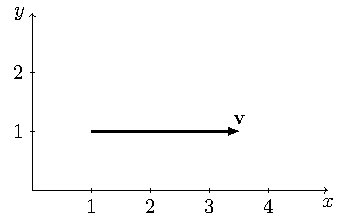
\includegraphics{vectorBaseAtPointOfAction}
\caption{سمتیہ}
\label{شکل_سمتیہ_دم_پر_عمل_درامد_ہوتی_ہے}
\end{figure}

\حصہ{سمتی الجبرا}
دو سمتیوں کا ترسیمی  مجموعہ حاصل کرنے کی خاطر ایک سمتیہ کے سر کو دوسری سمتیہ کے دُم  کے ساتھ ملایا جاتا ہے۔پہلی سمتیہ کی دُم سے دوسری سمتیہ کے سر تک سمتیہ حاصل جمع ہو گا۔اس عمل کو شکل \حوالہ{شکل_سمتیہ_سمتیوں_کا_مجموعہ}-الف میں دکھایا گیا ہے۔شکل میں \سمتیہ{A} کے سر کے ساتھ \سمتیہ{B} کی دُم ملائی گئی ہے۔دو سے زیادہ سمتیوں کا مجموعہ بھی اسی عمل کو استعمال کرتے  ہوئے حاصل کیا جاتا ہے۔اس عمل کو \اصطلاح{سر سے دُم جوڑنا}\فرہنگ{سر سے دُم جوڑنا}\فرہنگ{head to tail rule}\حاشیہب{head to tail rule} کہتے ہیں۔شکل \حوالہ{شکل_سمتیہ_سمتیوں_کا_مجموعہ}-ب میں دو سمتیوں کے دُم ملا کر سمتیوں کے متوازی الاضلاع\فرہنگ{متوازی الاضلاع}\حاشیہب{parallelogram law}\فرہنگ{parallelogram law}  سے ان کا مجموعہ حاصل کرنا دکھایا گیا ہے جسے دیکھ کر صاف ظاہر ہے کہ $\bf{A}+\bf{B}=\bf{B}+\bf{A}$ ہے یعنی سمتیوں کا مجموعہ قانون تبادل\فرہنگ{قانون تبادل}\حاشیہب{commutative law}\فرہنگ{commutative law} پر پورا اترتا ہے۔اسی طرح سمتیوں کا مجموعہ قانون تلازمی\فرہنگ{قانون تلازمی}\حاشیہب{associative law}\فرہنگ{associative law}
\begin{align}
\bf{A}+\left(\bf{B}+\bf{C}\right)=\left(\bf{A}+\bf{B}\right)+\bf{C}
\end{align}
 پر بھی پورا اترتا ہے۔
%  
\begin{figure}
\begin{subfigure}{0.5\textwidth}
\centering
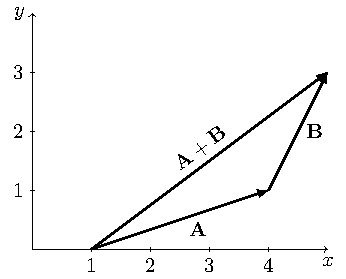
\includegraphics{figVectorHeadToTailRule}
\caption{سر کے ساتھ دُم جوڑ کر مجموعہ حاصل کیا جاتا ہے۔}
%\label{شکل_سمتیہ_سر_دم_جوڑنا}
\end{subfigure}
%
\begin{subfigure}{0.5\textwidth}
\centering
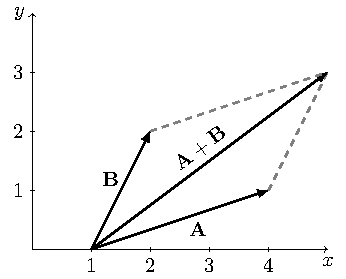
\includegraphics{figVectorParallelogramAdditionLaw}
\caption{متوازی الاضلاع سے بھی مجموعہ حاصل کیا جاتا ہے۔}
%\label{شکل_سمتیہ_متوازی_الاضلاع}
\end{subfigure}
\caption{سمتیوں کے مجموعے کا حصول}
\label{شکل_سمتیہ_سمتیوں_کا_مجموعہ}
\end{figure}

سمتیوں کے تفریق کا اصول  جمع کے اصول سے حاصل کیا جا سکتا ہے۔ہم $\bf{A}-\bf{B}$ کو $\bf{A}+\left(-\bf{B}\right)$ لکھ سکتے ہیں جہاں $-\bf{B}$ سے مراد یہ ہے کہ سمتیہ $\bf{B}$ کی سمت الٹی کر دی گئی ہے۔یوں $\bf{A}-\bf{B}$ حاصل کرنے کی خاطر $\bf{B}$ کی سمت الٹی کرتے ہوئے اس نئے سمتیہ کو $\bf{A}$ کے ساتھ جمع کیا جاتا ہے۔

سمتیہ \سمتیہ{A} کو مثبت  مقداری \عددیء{k} سے ضرب دینے سے سمتیہ کی سمت پر کوئی اثر نہیں ہوتا جبکہ اس کی لمبائی \عددیء{k} گنا ہو جاتی ہے۔اس کے برعکس سمتیہ \سمتیہ{A} کو منفی مقداری \عددیء{-k} سے ضرب دینے سے سمتیہ کی سمت الٹ ہو جاتی ہے اور اس کی لمبائی \عددیء{\abs{k}} گنا ہو جاتی ہے۔

دو سمتیے اُس صورت میں برابر ہوتے ہیں جب ان کا تفریق صفر کے برابر ہو یعنی \عددیء{\kvec{A}=\kvec{B}} تب ہو گا جب \عددیء{\kvec{A}-\kvec{B}=0} ہو۔

ہم سمتی میدان کے متغیرات کو آپس میں جمع یا منفی صرف اُس صورت کریں گے جب یہ متغیرات ایک ہی نقطے پر بیان کئے گئے ہوں۔یوں کسی بھی نقطے پر دو یا دو سے زیادہ مقناطیسوں کا اجتماعی مقناطیسی میدان حاصل کرتے ہوئے اس نقطے پر تمام مقناطیسوں کا علیحدہ علیحدہ مقناطیسی میدان لیتے ہوئے ان کا مجموعہ لیا جائے گا۔

اگر ہم سمتی میدان کی بات نہ کر رہے ہوں تب ہم مختلف مقامات پر پائے جانے والے سمتیوں کا بھی مجموعہ یا فرق لے سکتے ہیں۔یوں سمندر کے پانی میں ڈوبے  آب دوز کی اوپر اور نچلی سطح پر قوت کا مجموعہ حاصل کرتے ہوئے ہم یہ معلوم کر سکتے ہیں کہ آیا یہ مزید ڈوبے گا یا نہیں۔  

\حصہ{کارتیسی محدد}\شناخت{حصہ_سمتیہ_کارتیسی_محدد}
ایسا طریقہ جس سے کسی نقطے کا مقام بیان کیا جائے محدد\فرہنگ{محدد}\حاشیہب{coordinates}\فرہنگ{coordinates} کہلاتا ہے۔سیدھی سطح پر کسی بھی نقطے کو دو محدد سے ظاہر کیا جا سکتا ہے۔خلاء تین طرفہ\حاشیہب{three dimensional} ہے لہٰذا خلاء میں کسی بھی نقطے کو تین محدد سے ظاہر کیا جا سکتا ہے۔شکل \حوالہ{شکل_سمتیہ_اکائی_سے_سمتیہ_کا_اظہار}-الف میں دو طرفہ  \اصطلاح{کارتیسی} محدد پر اکائی لمبائی کے دو سمتیات \عددیء{\ax} اور \عددیء{\ay} دکھائے گئے ہیں۔اکائی سمتیہ \عددیء{\ax} کی سمت مثبت \عددیء{x} جانب کو ہے جبکہ \عددیء{\ay}  کی سمت مثبت \عددیء{y} جانب کو ہے۔شکل-ب میں \سمتیہ{A} دکھایا گیا ہے۔کسی بھی سمتیہ کو دو یا دو سے زیادہ سمتیوں کے مجموعے کی شکل میں لکھا جا سکتا ہے۔شکل میں \عددیء{\kvec{A}} کو \عددیء{\kvec{A}_x} اور \عددیء{\kvec{A}_y} کے مجموعے کی شکل میں دکھایا گیا ہے یعنی
\begin{align}
\kvec{A}=\kvec{A}_x+\kvec{A}_y
\end{align}

\begin{figure}
\begin{subfigure}{0.5\textwidth}
\centering
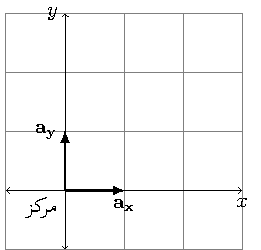
\includegraphics{unitVectorsInTwoDimensionalCartesianSpace}
\caption{اکائی سمتیہ}
%\label{شکل_سمتیہ_سر_دم_جوڑنا}
\end{subfigure}
%
\begin{subfigure}{0.5\textwidth}
\centering
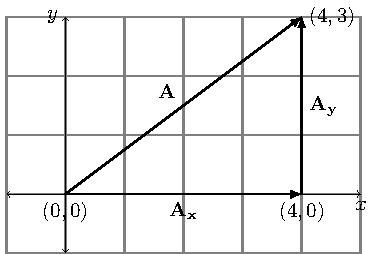
\includegraphics{vectorsRepresentationCartesianSpace}
\caption{اکائی سمتیوں کی مدد سے کسی بھی سمتیہ کو ظاہر کیا جا سکتا ہے۔}
%\label{شکل_سمتیہ_متوازی_الاضلاع}
\end{subfigure}
\caption{اکائی سمتیہ اور ان کا استعمال}
\label{شکل_سمتیہ_اکائی_سے_سمتیہ_کا_اظہار}
\end{figure}
%


زمین کی سطح کو لامحدود سیدھی سطح تصور کرتے ہوئے اس پر دو عمودی لکیریں کھینچتے ہوئے ایک لکیر کو \عددیء{x} محدد اور دوسری لکیر کو \عددیء{y} محدد تصور کیا جا سکتا ہے۔ایسی صورت میں اونچائی کو \عددیء{z} محدد سے ظاہر کیا جائے گا۔ اب اگر اونچائی صفر رکھتے ہوئے \عددیء{x} اور \عددیء{y} کو تبدیل کیا جائے تو ہم زمین کی سطح پر حرکت کریں گے۔اس طرح ہم دیکھتے ہیں کہ زمین کی سطح پر \عددیء{z=0} جبکہ اس پر \عددیء{x} اور \عددیء{y} آزاد متغیرات ہیں۔یوں زمین کی سطح کو \عددیء{z=0} سطح کہتے ہیں جسے
\begin{align*}
z=0, \quad  x\le \abs{\mp \infty}, \quad y \le \abs{\mp \infty}
\end{align*} 
لکھا جا سکتا ہے۔  شکل \حوالہ{شکل_سمتیہ_کارتیسی_نقطہ_اور_عمودی_سطحیں}-الف میں اس سطح کی نشاندہی کی گئی ہے۔ہم بالکل اسی طرح \عددیء{y=0} سطح اور \عددیء{x=0} سطح بھی بیان کر سکتے ہیں۔

\begin{figure}
\begin{subfigure}{0.5\textwidth}
\centering
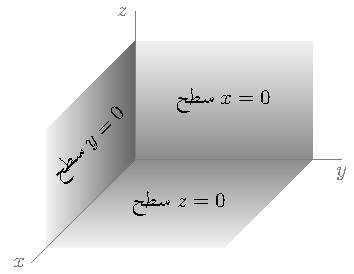
\includegraphics{figVectorPlaneSurfacesCartesian}
\caption{کارتیسی محدد میں عمودی سیدھی سطحیں۔}
\label{شکل_سمتیہ_کارتیسی_عمودی-تین_سطحیں}
\end{subfigure}
%
\begin{subfigure}{0.5\textwidth}
\centering
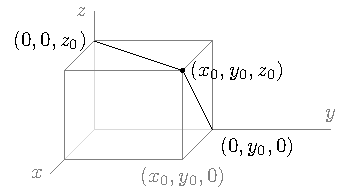
\includegraphics{figVectorPerpendicularsFromPointToCartesianAxis3D}
\caption{نقطے سے محدد پر عمود۔}
\label{شکل_سمتیہ_نقطے_سے_کارتیسی_محدد_پر_عمود}
\end{subfigure}
%
\caption{کارتیسی نظام میں نقطہ اور تین عمودی سطحیں۔}
\label{شکل_سمتیہ_کارتیسی_نقطہ_اور_عمودی_سطحیں}
\end{figure}
شکل  \حوالہ{شکل_سمتیہ_کارتیسی_نقطہ_اور_عمودی_سطحیں}-ب  کو دیکھتے ہوئے آگے  پڑھیں۔ کارتیسی محدد میں کسی بھی نقطے کو \عددیء{(x_0,y_0,z_0)} لکھا جا سکتا ہے۔اس نقطے تک پہنچنے کی خاطر  کارتیسی محدد کے مرکز سے پہلے \عددیء{x} محدد کے متوازی \عددیء{x_0}  فاصلہ طے کرتے ہوئے \عددیء{(x_0,0,0)} تک پہنچیں۔اس کے بعد \عددیء{y} محدد کے متوازی \عددیء{y_0} فاصلہ طے کرتے ہوئے \عددیء{(x_0,y_0,0)} تک پہنچیں  اور آخرکار \عددیء{z} محدد کے متوازی \عددیء{z_0} فاصلہ طے کرتے ہوئے درکار نقطہ \عددیء{(x_0,y_0,z_0)} تک پہنچیں۔اس عمل میں یہ ضروری نہیں کہ پہلے \عددیء{x} محدد کے متوازی ہی چلا جائے۔آپ مرکز سے پہلے \عددیء{y} محدد کے متوازی \عددیء{y_0} فاصلہ طے کرنے کے بعد \عددیء{z} محدد کے متوازی \عددیء{z_0} اور آخرکار \عددیء{x} محدد کے متوازی \عددیء{x_0} فاصلہ طے کرتے ہوئے بھی اسی نقطے تک پہنچ سکتے ہیں۔تینوں فاصلوں کو کسی بھی ترتیب سے طے کیا جا سکتا ہے۔

 نقطہ \عددیء{(x_0,y_0,z_0)} سے \عددیء{x} محدد پر عمود بناتے ہوئے  \عددیء{(x_0,0,0)} حاصل ہوتا ہے۔اسی طرح اس نقطے سے \عددیء{y} محدد پر عمود \عددیء{(0,y_0,0)} اور \عددیء{z} محدد پر عمود \عددیء{(0,0,z_0)} دیتا ہے۔نقطہ \عددیء{(x_0,y_0,z_0)} سے \عددیء{y} محدد اور \عددیء{z} محدد پر عمودی لکیریں گہری سیاہی میں دکھائے گئے ہیں۔ اگر \عددیء{(x_0,y_0,z_0)} سے  شروع ہوتے ہوئے \عددیء{z} محدد کے متوازی یوں چلا جائے کہ آخرکار \عددیء{z=0} ہو جائے تو نقطہ \عددیء{(x_0,y_0,0)} حاصل ہو گا۔ اب اگر یہاں سے \عددیء{x} محدد کے متوازی یوں چلا جائے کہ آخرکار \عددیء{x=0} ہو جائے تو نقطہ \عددیء{(0,y_0,0)} حاصل ہو گا۔یہ وہی نقطہ ہے جو \عددیء{(x_0,y_0,z_0)} سے \عددیء{y} محدد پر عمودی لکیر بناتے ہوئے حاصل ہوتا ہے۔اس عمل میں ہم پہلے \عددیء{x} محدد کے متوازی چلتے ہوئے \عددیء{x=0} کرنے کے بعد \عددیء{z} محدد کے متوازی چلتے ہوئے \عددیء{z=0} کرتے ہوئے بھی نقطہ \عددیء{(0,0,y_0)} تک پہنچ سکتے تھے۔

نقطہ \عددیء{(x_0,y_0,z_0)} تک قدر مختلف انداز سے بھی پہنچا جا سکتا ہے جسے کارتیسی محدد میں سمجھنا زیادہ آسان ہے۔فرض کریں کہ \عددیء{x=x_0} پر لامحدود \عددیء{yz} سیدھی سطح بنائی جائے۔ایسی سطح کو \عددیء{x=x_0} سطح  کہتے ہیں۔اس سطح کو
\begin{align*}
x=x_0, \quad  y\le \abs{\mp \infty}, \quad z \le \abs{\mp \infty}
\end{align*} 
لکھا جا سکتا ہے۔اس مساوات میں \عددیء{x_0} مقررہ ہے جبکہ \عددیء{y} اور \عددیء{z} متغیرات ہیں۔دو متغیرات کی مساوات سطح کو ظاہر کرتی ہے۔اگر \عددیء{y=y_0} پر لامحدود \عددیء{xz} سیدھی سطح بنائی جائے تو یہ دو سطحے  آپس میں سیدھی لکیر پر ملیں گے۔یہ لکیر
\begin{align*}
x=x_0, \quad  y=y_0, \quad z \le \abs{\mp \infty}
\end{align*} 
لکھی جا سکتی ہے۔اس مساوات میں \عددیء{x_0} اور \عددیء{y_0} مقررہ ہیں جبکہ \عددیء{z} متغیرہ ہے۔ایک متغیرہ کی مساوات لکیر کو ظاہر کرتی ہے۔اب اگر \عددیء{z=z_0} پر لامحدود \عددیء{xy} سیدھی سطح بھی بنائی جائے تب یہ تینوں سطحے ایک نقطے \عددیء{N(x_0,y_0,z_0)} پر آپس کو چھوئنگے۔یہ صورت حال شکل \حوالہ{شکل_سمتیہ_تین_عمودی_سطحوں_سے_نقطہ} میں دکھائی گئی ہے جہاں لامحدود سطحوں کے کچھ حصے دکھائے گئے ہیں۔آپ دیکھیں گے کہ نقطے تک پہنچنے کا یہ طریقہ دیگر محدد میں استعمال کرنا لازمی ثابت ہو گا۔
\begin{figure}
\centering
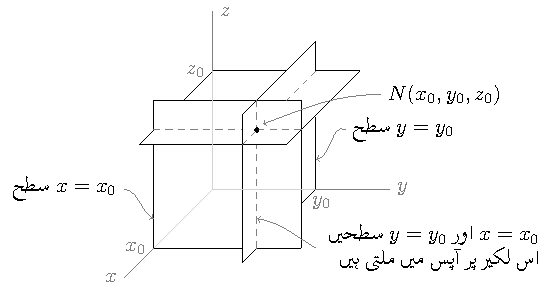
\includegraphics{figVectorLineAsSurfacesTouching}
\caption{تین عمودی سطحوں سے نقطے کا حصول۔}
\label{شکل_سمتیہ_تین_عمودی_سطحوں_سے_نقطہ}
\end{figure}

اگر سطح \عددیء{x=x_0}  کے متوازی \عددیء{x=x_0+\dif x} پر اور اسی طرح \عددیء{y=y_0} کے متوازی \عددیء{y=y_0+\dif y} اور \عددیء{z=z_0} کے متوازی \عددیء{z=z_0+\dif z} سطح رکھے جائیں تو یہ چھ سطحے ایک چھوٹی  مکعب نما حجم  کو گھیریں گی جسے شکل \حوالہ{شکل_سمتیہ_کارتیسی_چھوٹی_مکعب} میں دکھایا گیا ہے جبکہ یہ تین نئی سطحیں آپس میں نقطہ \عددیء{N'(x_0+\dif x,y_0+\dif y,z_0+\dif z)} پر ملیں گی ۔
\begin{figure}
\centering
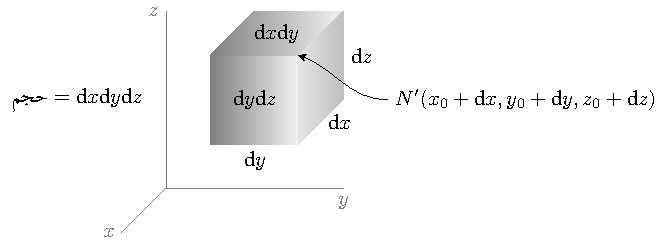
\includegraphics{figVectorCubeShaded}
\caption{چھ سطحے مکعب گھیرتی ہیں۔}
\label{شکل_سمتیہ_کارتیسی_چھوٹی_مکعب}
\end{figure}
اس مکعب نما کے اطراف \عددیء{\dif x}، \عددیء{\dif y} اور \عددیء{\dif z} ہیں۔ اس کی اوپر والی سطح کا رقبہ \عددیء{\dif x \dif y} ہے۔اسی طرح اس کی نچلی سطح کا رقبہ بھی \عددیء{\dif x \dif y} ہے۔سامنے سطح  اور پچھلی سطح دونوں \عددیء{\dif y \dif z} رقبے رکھتے ہیں جبکہ بائیں  اور دائیں سطحوں کے رقبے \عددیء{\dif x \dif z} کے برابر ہیں۔اس مکعب نما کی حجم \عددیء{\dif x \dif y \dif z} ہے۔نقطہ \عددیء{N'(x_0+\dif x,y_0+\dif y,z_0+\dif z)} شکل میں دکھایا گیا ہے جبکہ
 نقطہ \عددیء{N(x_0,y_0 ,z_0)} مکعب نما کا وہ واحد کونا ہے جسے شکل میں نہیں دکھایا گیا۔ان دو نقطوں کے درمیان فاصلہ \عددیء{NN'=\sqrt{\dif x^2+\dif y^2+\dif z^2}} ہے۔ 
%==================
\حصہ{اکائی سمتیات}
حصہ  \حوالہ{حصہ_سمتیہ_کارتیسی_محدد} کے شروع میں دو طرفہ کارتیسی نظام  میں سیدھی سطح پر کسی بھی سمتیہ کو دو سمتیات کی صورت میں لکھنا دکھایا گیا۔یہی طریقہ تین طرفہ کارتیسی نظام کے لئے بھی استعمال کیا جاتا ہے۔ تین طرفہ کارتیسی نظام کے تین اکائی سمتیات \عددیء{\ax}، \عددیء{\ay} اور \عددیء{\az} لکھے جاتے ہیں۔یہ تینوں سمتیات آپس میں عمودی ہیں۔کسی بھی اکائی سمتیہ کی طرح یہ تین اکائی سمتیات اکائی لمبائی رکھتے ہیں۔ \عددیء{\ax} کی سمت \عددیء{x} محدد کے بڑھتے جانب کو ہے۔اسی طرح \عددیء{\ay} کی سمت \عددیء{y} محدد کے بڑھتے جانب کو اور \عددیء{\az} کی سمت \عددیء{z} محدد کے بڑھتے جانب کو ہے۔شکل \حوالہ{شکل_سمتیہ_کارتیسی_تین_اکائی_سمتیات}-الف میں یہ تینوں اکائی سمتیات دکھائے گئے ہیں۔اسی شکل میں نقطہ \عددیء{(0,1,2)} پر سمتیہ دکھایا گیا ہے جس کی لمبائی دو کے برابر ہے جبکہ یہ اکائی سمتیہ \عددیء{\ay} کی سمت میں ہے۔اس سمتیہ کو \عددیء{2\ay} لکھا جا سکتا ہے۔یاد رہے کہ ایسے دو سمتیات برابر ہوتے ہیں جن کا طول برابر ہو اور جو ایک ہی سمت میں ہوں۔ یوں سمت تبدیل کئے بغیر سمتیہ کو کارتیسی محدد کے مرکز منتقل کرتے ہوئے اس کی قیمت نسبتاً آسانی سے لکھی جا سکتی ہے۔
\begin{figure}
\centering
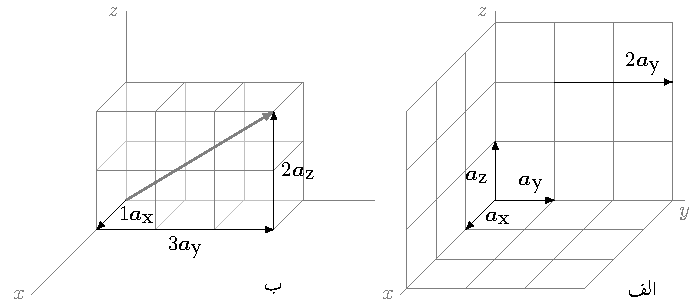
\includegraphics{figVector3DUnitVectors}
\caption{کارتیسی نظام کے اکائی سمتیات اور ان کا استعمال}
\label{شکل_سمتیہ_کارتیسی_تین_اکائی_سمتیات}
\end{figure}
%
\begin{figure}
\centering
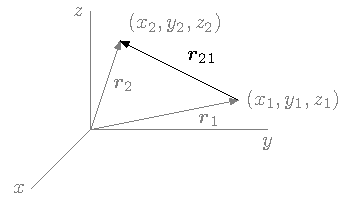
\includegraphics{figVector3DcartesianVectorEquation}
\caption{کارتیسی نظام میں سمتیہ کی مساوات کا حصول}
\label{شکل_سمتیہ_کارتیسی_سمتیہ_کی_مساوات}
\end{figure}
%
\begin{figure}
\centering
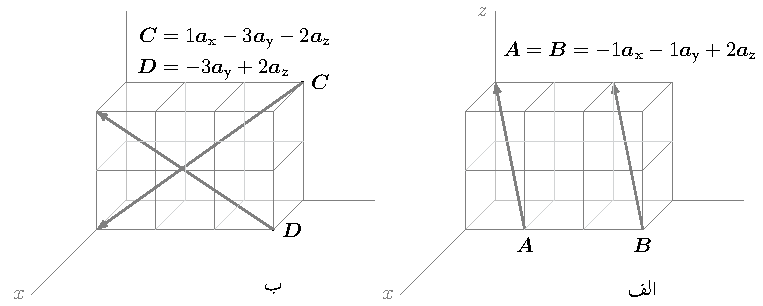
\includegraphics{figVector3DcartesianVectors}
\caption{کارتیسی نظام میں چند سمتیات}
\label{شکل_سمتیہ_کارتیسی_چند_سمتیات}
\end{figure}
%

شکل \حوالہ{شکل_سمتیہ_کارتیسی_سمتیہ_کی_مساوات} میں  مرکز سے \عددیء{(x_1,y_1,z_1)} تک سمتیہ \عددیء{\kvec{r}_1=x_1 \ax+y_1\ay+z_1\az} اور  مرکز سے \عددیء{(x_2,y_2,z_2)} تک سمتیہ \عددیء{\kvec{r}_2=x_2 \ax+y_2\ay+z_2\az} دکھائے گئے ہیں۔شکل میں سمتیہ \عددیء{\kvec{r}_{21}} بھی دکھائی گئی ہے جس کی دُم  \عددیء{(x_1,y_1,z_1)} اور  نوک \عددیء{(x_2,y_2,z_2)} پر ہے۔ سر سے دُم جوڑنے کے اصول کے استعمال سے \عددیء{\kvec{r}_2=\kvec{r}_{21}+\kvec{r}_1} لکھا جا سکتا ہے جس سے 
\begin{gather}
\begin{aligned}\label{مساوات_سمتیہ_کارتیسی_نظام_میں_قیمت}
\kvec{r}_{21}&=\kvec{r}_2-\kvec{r}_1\\
&=(x_2-x_1) \ax+(y_2-y_1)\ay+(z_2-z_1)\az
\end{aligned}
\end{gather}
حاصل ہوتا ہے۔اس مساوات کے استعمال سے سمتیہ کی مساوات باآسانی حاصل ہوتی ہے۔سمتیہ \عددیء{\kvec{r}_{21}} لکھتے ہوئے زیرنوشت میں سمتیہ کی نوک کو \عددیء{2} اور اس کی دُم  کو \عددیء{1} سے ظاہر کیا گیا ہے۔اس کتاب میں سمتیہ لکھتے ہوئے نوک اور دُم  کو اسی ترتیب سے زیرنوشت میں لکھا جائے گا۔یوں سمتیہ \عددیء{\kvec{r}_{21}} کو تین اجزاء \عددیء{(x_2-x_1)\ax}، \عددیء{(y_2-y_1)\ay} اور \عددیء{(z_2-z_1)\az} کے مجموعے کی شکل میں لکھا جا سکتا ہے۔

شکل \حوالہ{شکل_سمتیہ_کارتیسی_تین_اکائی_سمتیات}-ب میں مرکز سے \عددیء{(1,3,2)} تک سمتیہ دکھایا گیا ہے۔آپ دیکھ سکتے ہیں کہ اس کو تین سمتیات کا مجموعہ لکھا جا سکتا ہے یعنی \عددیء{1\ax+3\ay+2\az} جہاں اکائی سمتیات استعمال کرتے ہوئے تینوں اجزاء کو لکھا گیا ہے۔ سمتیہ کی دُم \عددیء{(0,0,0)} اور اس کی نوک \عددیء{(1,3,2)} پر لیتے ہوئے  یہی جواب  مساوات \حوالہ{مساوات_سمتیہ_کارتیسی_نظام_میں_قیمت} سے بھی حاصل ہوتا ہے۔

شکل \حوالہ{شکل_سمتیہ_کارتیسی_چند_سمتیات}-الف میں دو متوازی سمتیات \عددیء{\kvec{A}} اور \عددیء{\kvec{B}} دکھائے ہیں جن کی لمبائی برابر ہے۔ چونکہ ان کی لمبائی برابر ہے اور یہ دونوں ایک ہی سمت میں ہیں لہٰذا \عددیء{\kvec{A}=\kvec{B}=-1\ax-1\ay+2\az} لکھا جائے گا۔شکل \حوالہ{شکل_سمتیہ_کارتیسی_چند_سمتیات}-ب میں \عددیء{\kvec{C}} کی دُم سے \عددیء{\ax} جانب ایک قدم اور یہاں سے \عددیء{-\ay} جانب تین قدم اور آخرکار \عددیء{-\az} جانب دو قدم چلنے سے اس کی نوک تک پہنچا جا سکتا ہے لہٰذا \عددیء{\kvec{C}=1\ax-3\ay-2\az} لکھا جائے گا۔ اسی طرح \عددیء{\kvec{D}} کی دُم سے  \عددیء{-\ay} جانب تین قدم اور پھر \عددیء{\az} جانب دو قدم چلتے ہوئےسمتیہ کی نوک تک پہنچا جایا سکتا ہے لہٰذا \عددیء{\kvec{D}=-3\ay+2\az} لکھا جائے گا۔سمتیہ \عددیء{\kvec{D}} کو دو اجزاء کی شکل میں لکھا گیا ہے چونکہ اس کے تیسرے جزو کی لمبائی صفر کے برابر ہے۔
%=====================
\ابتدا{مشق}
مساوات \حوالہ{مساوات_سمتیہ_کارتیسی_نظام_میں_قیمت} کے استعمال سے شکل \حوالہ{شکل_سمتیہ_کارتیسی_چند_سمتیات} میں تمام سمتیات لکھیں۔

جوابات:تمام جوابات شکل میں دئے گئے ہیں۔
\انتہا{مشق}
%======================
\begin{figure}
\centering
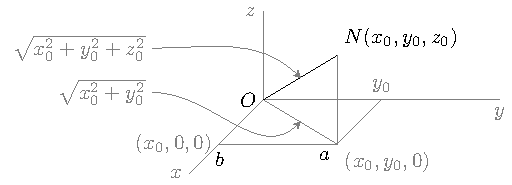
\includegraphics{figVectorCartesianAmplitudeFromPythagorousTheorem}
\caption{کارتیسی نظام میں سمتیہ کا طول}
\label{شکل_سمتیہ_کارتیسی_سمتیہ_طول}
\end{figure}

شکل \حوالہ{شکل_سمتیہ_کارتیسی_سمتیہ_طول} میں مرکز سے نقطہ \عددیء{N(x_0,y_0,z_0)} تک کا فاصلہ \عددیء{ON} مسئلہ \اصطلاح{فیثاغورث}\فرہنگ{فیثاغورث}\حاشیہب{Pythagoras theorem}\فرہنگ{Pythagoras theorem} سے حاصل کیا جا سکتا ہے۔اس نقطے سے \عددیء{z=0} سطح پر عمود سے نقطہ \عددیء{a} حاصل ہوتا ہے۔نقطہ \عددیء{a} سے \عددیء{x} محدد پر عمود نقطہ \عددیء{b} دیتا ہے۔تکون \عددیء{Oba} میں \عددیء{O} سے \عددیء{b} کا فاصلہ \عددیء{x_0} ہے جبکہ \عددیء{b} سے \عددیء{a} کا فاصلہ \عددیء{y_0} ہے۔یوں فاصلہ \عددیء{Oa} مسئلہ فیثاغورث کی مدد سے  \عددیء{\sqrt{x_0^2+y_0^2}} کے برابر ہو گا۔ تکون \عددیء{OaN} میں \عددیء{a} پر \عددیء{90^{\circ}} کا زاویہ پایا جاتا ہے۔یوں مسئلہ فیثاغورث کی مدد سے \عددیء{ON} کا فاصلہ \عددیء{\sqrt{x_0^2+y_0^2+z_0^2}} حاصل ہوتا ہے۔

مساوات \حوالہ{مساوات_سمتیہ_کارتیسی_نظام_میں_قیمت} سمتیہ کی عمومی مساوات ہے۔اس میں دئے سمتیہ \عددیء{\kvec{r}_{21}} کی دُم محدد کے مرکز پر رکھنے سے صاف ظاہر ہے کہ سمتیہ کی مقدار
\begin{align}
\abs{\kvec{r}_{21}}=r_{21}=\sqrt{(x_2-x_1)^2+(y_2-y_1)^2+(z_2-z_1)^2}
\end{align}
کے برابر ہے۔اگر سمتیہ کو اس کی مقدار سے تقسیم کیا جائے تو حاصل جواب کی مقدار اکائی ہو گی جبکہ اس کی سمت میں کوئی تبدیلی رونما نہیں ہو گی۔یوں  \عددیء{\kvec{r}_{21}} کو \عددیء{\abs{\kvec{r}_{21}}} سے تقسیم کرتے ہوئے \عددیء{\kvec{r}_{21}} کی سمت میں اکائی سمتیہ \عددیء{\kvec{a}_{r21}} حاصل کی جا سکتی ہے۔
\begin{align}
\kvec{a}_{r21}=\frac{\kvec{r}_{21}}{\abs{\kvec{r}_{21}}}=\frac{(x_2-x_1) \ax+(y_2-y_1)\ay+(z_2-z_1)\az}{\sqrt{(x_2-x_1)^2+(y_2-y_1)^2+(z_2-z_1)^2}}
\end{align}
یاد رہے کہ سمتیہ کی سمت اور طول تبدیل کئے بغیر اسے ایک مقام سے دوسری مقام منتقل کیا جا سکتا ہے۔البتہ وہ سمتیہ جو کسی نقطے کی مقام تعین کرتا ہو کو اگر کہیں اور منتقل کیا جائے تو ایسی صورت میں  سمتیہ کی نوک درکار نقطے پر نہیں رہے گی۔اسی حقیقت کی بنا پر میدان ظاہر کرنے والے سمتیہ کو اپنی جگہ سے نہیں ہٹایا جا سکتا۔میدانی سمتیہ کی دُم اس مقام پر پائی جاتی ہے جہاں میدان بیان کی جا رہی ہو۔  

سمتیات کے استعمال سے نقطہ \عددیء{(x,y,z)} کے مقام کو \عددیء{\kvec{r}=x\ax+y\ay+z\az} لکھا جاتا ہے۔کسی بھی سمتیہ مثلاً قوت \عددیء{\kvec{F}} کو بالکل اسی طرح  \عددیء{\kvec{F}=F_x\ax+F_y\ay+F_z\az} لکھا جاتا ہے جہاں \عددیء{F_x \ax}، \عددیء{F_y \ay} اور \عددیء{F_z\az} اس کے تین اجزاء ہیں۔اس طرح قوت کی مقدار  \عددیء{\abs{\kvec{F}}=\sqrt{F_x^2+F_y^2+F_z^2}} کے برابر ہو گی۔
%======================
\ابتدا{مثال}
نقطہ \عددیء{(-5,2,-1)}  کا مقام ظاہر کرنے والا سمتیہ اور اس سمتیہ کا طول حاصل کریں۔اسی سمتیہ کی سمت میں اکائی سمتیہ حاصل کریں۔

حل:مرکز سے اس نقطے تک کا سمتیہ \عددیء{\kvec{r}=-5\ax+2\ay-1\az} ہے جبکہ اس سمتیہ  کا طول \عددیء{\abs{\kvec{r}}=\sqrt{5^2+2^2+1^1}=\sqrt{30}} ہے۔یوں اکائی سمتیہ \عددیء{\kvec{a}_r=\tfrac{-5\ax+2\ay-1\az}{\sqrt{30}}} ہو گا۔
\انتہا{مثال}
%=====================

\ابتدا{مثال}\شناخت{مثال_سمتیہ_نقطے_سے_درمیان_تک_سمتیہ}
شکل \حوالہ{شکل_سمتیہ_استعمال_سمتیہ_مثال} میں تین نقطے \عددیء{M(1,6,4)}، \عددیء{N(4,5,1)} اور \عددیء{P(1,2,2)} دئے گئے ہیں۔\عددیء{M} اور \عددیء{N} کے درمیان سیدھی لکیر پر \عددیء{M} سے کل فاصلے کے  \عددیء{\tfrac{1}{3}} پر نقطہ \عددیء{Q} پایا جاتا ہے۔\عددیء{Q} سے \عددیء{P} تک سمتیہ حاصل کرتے ہوئے ان دو نقطوں کے درمیان فاصلہ معلوم کریں۔
\begin{figure}
\centering
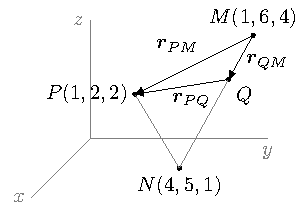
\includegraphics{figVectorExampleA}
\caption{سمتیوں کا استعمال}
\label{شکل_سمتیہ_استعمال_سمتیہ_مثال}
\end{figure}
حل:\عددیء{M} سے \عددیء{N} تک سمتیہ
\begin{align*}
\kvec{r}_{NM}&=(4-1)\ax+(5-6)\ay+(1-4)\az\\
&=3\ax-1\ay-3\az
\end{align*}
ہے۔\عددیء{M} سے \عددیء{Q} تک سمتیہ \عددیء{\kvec{r}_{QM}} اور \عددیء{\kvec{r}_{NM}} ایک ہی سمت میں ہیں جبکہ \عددیء{\abs{\kvec{r}_{QM}}=\tfrac{1}{3}\abs{\kvec{r}_{NM}}} کے برابر ہے۔یوں
\begin{align*}
\kvec{r}_{QM}=\frac{1}{3}\kvec{r}_{NM}=\frac{1}{3}(3\ax-1\ay-3\az)=1\ax-\frac{1}{3}\ay-1\az
\end{align*}
ہو گا۔\عددیء{M} سے \عددیء{P} تک سمتیہ
\begin{align*}
\kvec{r}_{PM}&=(1-1)\ax+(2-6)\ay+(2-4)\az\\
&=-4\ay-2\az
\end{align*}
ہے۔شکل کو دیکھتے ہوئے ہم لکھ سکتے ہیں \عددیء{\kvec{r}_{QM}+\kvec{r}_{PQ}=\kvec{r}_{PM}} لہٰذا
\begin{align*}
\kvec{r}_{PQ}&=\kvec{r}_{PM}-\kvec{r}_{QM}\\
&=(-4\ay-2\az)-(1\ax-\frac{1}{3}\ay-1\az)\\
&=-1\ax-\frac{11}{3}\ay-1\az
\end{align*}
ہو گا۔\عددیء{Q} سے \عددیء{P} تک فاصلہ \عددیء{\sqrt{1^1+\left(\tfrac{11}{3}\right)^2+1^2}=3.93} ہے۔
\انتہا{مثال}
%===================
\ابتدا{مشق}
مثال \حوالہ{مثال_سمتیہ_نقطے_سے_درمیان_تک_سمتیہ} میں دئے نقطوں کو استعمال کرتے ہوئے \عددیء{M} سے \عددیء{P} تک سمتیہ حاصل کریں۔اسی طرح \عددیء{P} سے \عددیء{N} تک سمتیہ اور \عددیء{M} سے \عددیء{N} تک سمتیہ حاصل کریں۔پہلے دو جوابات کو استعمال کرتے ہوئے \اصطلاح{سر سے دُم جوڑنے} کے اصول سے تیسرا سمتیہ دوبارہ حاصل کریں۔

جوابات:\عددیء{-5\ax-4\ay} ، \عددیء{-1\ax+4\ay+12\az} اور \عددیء{-6\ax+12\az}

\انتہا{مشق}


\حصہ{میدانی سمتیہ}\حاشیہط{لکھنا ہے}

\حصہ{سمتی رقبہ}
کسی بھی سطح کے دو اطراف ہوتے ہیں۔یوں سطح کے کسی بھی نقطے پر دو آپس میں الٹ سمتوں میں عمود بنائے جا سکتے ہیں۔سیدھی سطح جس کا رقبہ \عددیء{S} ہو کے ایک طرف پر اکائی عمود \عددیء{\kvec{a}_N} اور دوسری طرف پر اکائی عمود \عددیء{-\kvec{a}_N} بنائے جا سکتے ہیں۔اگر ان دو عمود میں سے ایک عمود مثلاً \عددیء{\kvec{a}_N} کو سطح کی سمت\حاشیہد{عمود سطح کے ساتھ نوے درجہ زاویہ بناتا ہے۔\عددیء{\kvec{a}_N} کے زیر نوشت میں \عددیء{N}، لفظ \موٹا{نوے} کے پہلے حرف کی آواز کو ظاہر کرتا ہے۔} تصور کیا جائے تب اس سطح کا \اصطلاح{سمتی رقبہ}\فرہنگ{سمتی رقبہ}\حاشیہب{vector area}\فرہنگ{vector area} \عددیء{S\kvec{a}_N} ہو گا۔بند سطح کے  بیرونی اکائی عمود کو سطح کی سمت تصور کیا جاتا ہے۔شکل \حوالہ{شکل_سمتیہ_سمتی_رقبہ} میں سمتی رقبے \عددیء{\kvec{A}_1} اور \عددیء{\kvec{A}_2} دکھائے گئے ہیں جہاں بند سطح کے بیرونی عمود کو ہی سطح کی سمت دکھایا گیا ہے۔
\begin{figure}
\centering
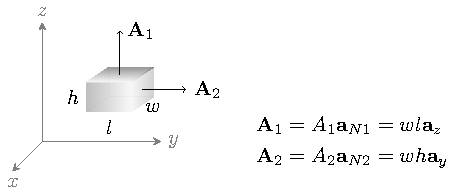
\includegraphics{figVectorVectorArea}
\caption{سمتی رقبہ}
\label{شکل_سمتیہ_سمتی_رقبہ}
\end{figure}


\حصہ{غیر سمتی ضرب}
دو سمتیات \عددیء{\kvec{A}} اور \عددیء{\kvec{B}} کے \اصطلاح{غیر سمتی ضرب}\فرہنگ{غیر سمتی ضرب}\فرہنگ{نقطہ ضرب}\فرہنگ{مقداری ضرب}\حاشیہب{scalar product}\فرہنگ{scalar product} سے مراد \عددیء{\kvec{A}} کی مقدار ضربِ  \عددیء{\kvec{B}} کی مقدار ضربِ سمتیوں کے مابین چھوٹے زاویے کا کوسائن ہے۔
\begin{align}\label{مساوات_سمتیہ_مقداری_ضرب}
\kvec{A} \cdot \kvec{B}=\abs{\kvec{A}} \abs{\kvec{B}} \cos \theta_{AB}
\end{align}

اگر دونوں سمتیات کی دُم ایک ہی جگہ پر نہ ہو تب ان کے مابین زاویہ دریافت کرنے کی  خاطر سمتیوں کی سمت تبدیل کئے بغیر انہیں ایک نقطے پر منتقل کیا جا سکتا ہے۔غیر سمتی ضرب دو سمتیوں کے مابین کیا جاتا ہے جبکہ اس کا حاصل جواب مقداری ہوتا ہے جس کی وجہ سے اسے  \اصطلاح{مقداری ضرب} بھی کہا جاتا ہے۔غیر سمتی ضرب کو سمتیوں کے درمیان نقطے سے ظاہر کیا جاتا ہے۔اسی وجہ سے اسے \اصطلاح{ضرب نقطہ}\حاشیہب{dot product}\فرہنگ{dot product} بھی کہا جاتا ہے۔ یوں \عددیء{\kvec{A} \cdot \kvec{B}} کو "\عددیء{\kvec{A}}نقطہ \عددیء{\kvec{B}}" پڑھا جاتا ہے۔بالکل سادہ ضرب کی طرح \عددیء{\kvec{A} \cdot \kvec{B}} کو \عددیء{\kvec{B} \cdot \kvec{A}} بھی لکھا جا سکتا ہے یعنی غیر سمتی ضرب میں متغیرات کی ترتیب اہمیت نہیں رکھتی۔

کارتیسی اکائی سمتیات \عددیء{\ax}، \عددیء{\ay} اور \عددیء{\az} آپس میں عمودی ہیں لہٰذا ان میں کسی بھی دو سمتیات کے درمیان \عددیء{90 \degree} زاویہ پایا جاتا ہے۔چونکہ \عددیء{\cos 90=0} کے برابر ہوتا ہے لہٰذا ان میں کسی بھی دو سمتیوں کا غیر سمتی ضرب صفر کے برابر ہوتا ہے یعنی
\begin{align}\label{مساوات_سمتیہ_عمودی_نقطہ_ضرب_برابر_صفر_اجزاء}
\ax \cdot \ay =0, \quad \ax \cdot \az=0, \quad \ay \cdot \az=0
\end{align}
ایک ہی سمت میں دو سمتیوں کے درمیان صفر زاویہ ہوتا ہے اور \عددیء{\cos 0=1} کے برابر ہے۔ اکائی سمتیہ کا طول بھی ایک کے برابر ہے لہٰذا مساوات \حوالہ{مساوات_سمتیہ_مقداری_ضرب} کے تحت \عددیء{\ax} اور \عددیء{\ax} کا غیر سمتی ضرب
\begin{align*}
\ax \cdot \ax=(\abs{\ax})(\abs{\ax})(\cos 0\degree)=(1)(1)(1)=1
\end{align*}
ہو گا۔بقایا دو کارتیسی اکائی سمتیات کا خود غیر سمتی ضرب بھی ایک کے برابر ہے۔
\begin{align}\label{مساوات_سمتیہ_عمودی_نقطہ_ضرب_برابر_ایک_اجزاء}
\ax \cdot \ax=1, \quad \ay \cdot \ay=1, \quad \az \cdot \az=1
\end{align}
مساوات \حوالہ{مساوات_سمتیہ_عمودی_نقطہ_ضرب_برابر_صفر_اجزاء} اور مساوات \حوالہ{مساوات_سمتیہ_عمودی_نقطہ_ضرب_برابر_ایک_اجزاء} کو \اصطلاح{کرونیکر ڈیلٹا}\فرہنگ{کرونیکر ڈیلٹا}\حاشیہد{یہ لیوپولڈ کرونیکر کے نام سے  منسوب ہے۔} \عددیء{\delta_{ij}} کی مدد سے ایک ہی مساوات کی مدد سے یوں لکھا جا سکتا ہے۔
\begin{align}
\kvec{a}_i \cdot \kvec{a}_j=\delta_{ij}
\end{align}
جہاں
\begin{align}
\delta_{ij}=
\begin{cases}
0 \quad  \quad  i\ne j \; \textup{ اگر}\\
1 \quad \quad i=j \; \textup{ اگر}
\end{cases}
\end{align}
کے برابر ہے یعنی \عددیء{i=j} کی صورت میں ہی \عددیء{\delta_{ij}} کی قیمت ایک  جبکہ \عددیء{i\ne j} کی صورت میں ہی \عددیء{\delta_{ij}} کی قیمت صفر کے برابر لی جاتی ہے۔یوں \عددیء{\ax \cdot \ay} کی صورت میں \عددیء{i=\ax} جبکہ \عددیء{j=\ay} کے برابر ہیں۔یوں \عددیء{i} اور \عددیء{j} برابر نہیں ہیں لہٰذا حاصل جواب صفر کے برابر ہو گا۔اس کے برعکس \عددیء{\az \cdot \az} کی صورت میں \عددیء{i=\az} اور \عددیء{j=\az} ہیں لہٰذا \عددیء{i=j} ہے اور یوں حاصل جواب ایک کے برابر ہے۔

کارتیسی تین عمودی اکائیوں کی مدد سے سمتیات کا غیر سمتی ضرب نہایت آسانی سے حاصل ہوتا ہے۔یوں اگر \عددیء{\kvec{A}=A_x\ax+A_y\ay+A_z\az} اور  \عددیء{\kvec{B}=B_x\ax+B_y\ay+B_z\az}  دو سمتیات ہوں تب ان کا غیر سمتی ضرب
\begin{align*}
\kvec{A} \cdot \kvec{B}&=(A_x\ax+A_y\ay+A_z\az) \cdot (B_x\ax+B_y\ay+B_z\az)\\
&=A_x B_x \ax \cdot \ax+A_x B_y \ax \cdot \ay+A_x B_z \ax \cdot \az\\
& \quad \quad +A_y B_x \ay \cdot \ax+A_y B_y \ay \cdot \ay+A_y B_z \ay \cdot \az \\
&\quad \quad +A_z B_x \az \cdot \ax+A_z B_y \az \cdot \ay+A_z B_z \az \cdot \az
\end{align*}
ہو گا۔مساوات \حوالہ{مساوات_سمتیہ_عمودی_نقطہ_ضرب_برابر_صفر_اجزاء} اور مساوات \حوالہ{مساوات_سمتیہ_عمودی_نقطہ_ضرب_برابر_ایک_اجزاء} کا سہارا لیتے ہوئے یوں
\begin{align}\label{مساوات_سمتیہ_نقطہ_ضرب_بمدد_اکائی_سمتیات}
\kvec{A} \cdot \kvec{B}=A_x B_x+A_y B_y+ A_z B_z
\end{align}
حاصل ہوتا ہے۔اس مساوات سے ہم دیکھتے ہیں کہ سمتیہ \عددیء{\kvec{A}} کا خود غیر سمتی ضرب 
\begin{align}
\kvec{A} \cdot \kvec{A} =A_x^2+A_y^2+ A_z^2=\abs{\kvec{A}}^2
\end{align}
اس کے طول کے مربع کے برابر ہے۔یہ انتہائی اہم نتیجہ ہے جسے عموماً استعمال کرتے ہوئے سمتیہ کا طول حاصل کیا جاتا ہے۔

مساوات \حوالہ{مساوات_سمتیہ_مقداری_ضرب} اور مساوات \حوالہ{مساوات_سمتیہ_نقطہ_ضرب_بمدد_اکائی_سمتیات} کی مدد سے دو سمتیوں کے مابین زاویہ معلوم کیا جا سکتا ہے یعنی
\begin{align}
\theta_{AB}=\cos^{-1}\left(\frac{\kvec{A} \cdot \kvec{B}}{(\kvec{A} \cdot \kvec{A})(\kvec{B} \cdot \kvec{B})}\right)=\cos^{-1} \left(\frac{A_x B_x+A_y B_y+ A_z B_z}{\sqrt{A_x^2+A_y^2+A_z^2} \sqrt{B_x^2+B_y^2+B_z^2}} \right)
\end{align}
%==================
\ابتدا{مثال}
شکل \حوالہ{شکل_سمتیہ_استعمال_سمتیہ_مثال} میں تکون دکھایا گیا ہے جس کے نوک  \عددیء{M(1,6,4)}، \عددیء{N(4,5,1)} اور \عددیء{P(1,2,2)}  ہیں۔\عددیء{M} پر زاویہ حاصل کریں۔

حل:مثال  \حوالہ{مثال_سمتیہ_نقطے_سے_درمیان_تک_سمتیہ} میں  \عددیء{\kvec{r}_{NM}=3\ax-1\ay-3\az} اور \عددیء{\kvec{r}_{PM}=0\ax-4\ay-2\az} حاصل کئے گئے۔\عددیء{\abs{\kvec{r}_{NM}}=\sqrt{3^2+1^2+3^2}=\sqrt{19}}  اور \عددیء{\abs{\kvec{r}_{PM}}=\sqrt{4^2+2^2}=\sqrt{20}} ہیں جبکہ
\begin{align*}
\kvec{r}_{NM} \cdot \kvec{r}_{PM}=0+4+6=10
\end{align*}
کے برابر ہے۔یوں ان سمتیوں کے مابین زاویہ
\begin{align*}
\theta=\cos^{-1} \left(\frac{10}{\sqrt{19} \sqrt{20}} \right)=1.0321 \quad \si{\radian}
\end{align*}
یا \عددیء{59.137^\circ} ہے۔
\انتہا{مثال}
%======================
\begin{figure}
\centering
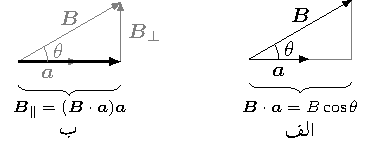
\includegraphics{figVectorComponentAlongUnitVector}
\caption{کسی بھی سمت میں سمتیہ کے جزو کا حصول۔}
\label{شکل_سمتیہ_کسی_سمت_میں_جزو}
\end{figure}
شکل \حوالہ{شکل_سمتیہ_کسی_سمت_میں_جزو}-الف میں سمتیہ \عددیء{\kvec{B}} اور اکائی سمتیہ \عددیء{\kvec{a}}  دکھائے گئے ہیں۔ان کا غیر سمتی ضرب
\begin{align*}
\kvec{B} \cdot \kvec{a} = \abs{\kvec{B}} \abs{\kvec{a}} \cos \theta=B \cos \theta
\end{align*}
کے برابر ہے۔شکل سے واضح ہے کہ یہی \عددیء{\kvec{a}} کی سمت میں \عددیء{\kvec{B}} کے جزو کا طول \عددیء{B_{\parallel}}\حاشیہد{\عددیء{B_{\parallel}} لکھتے ہوئے زیرنوشت میں دو متوازی لکیریں  یہ بتلاتی ہیں کہ \عددیء{\kvec{B}} کا یہ وہ حصہ ہے جو \عددیء{\kvec{a}} کے متوازی ہے۔اسی طرح عمودی مقدار کو عموماً \عددیء{\perp} کی علامت سے ظاہر کیا جاتا ہے۔} ہے۔یوں کسی بھی سمت میں \عددیء{\kvec{B}} کے جزو کا طول حاصل کرنے کی خاطر \عددیء{\kvec{B}} اور اس سمت کی اکائی سمتیہ کا غیر سمتی ضرب حاصل کریں۔یوں حاصل طول کا اکائی سمتیہ کے ساتھ ضرب یعنی \عددیء{(\kvec{B} \cdot \kvec{a}) \kvec{a}} سے اکائی سمتیہ کی سمت میں \عددیء{\kvec{B}} کا سمتی جزو  حاصل ہوتا ہے۔ شکل \حوالہ{شکل_سمتیہ_کسی_سمت_میں_جزو}-ب میں \عددیء{\kvec{a}} کی سمت میں \عددیء{\kvec{B}} کا سمتی جزو \عددیء{\kvec{B}_\parallel} دکھایا گیا ہے۔شکل سے واضح ہے کہ \عددیء{\kvec{B}} سے \عددیء{B_{\parallel} \kvec{a}} منفی کرنے سے  \عددیء{B_\perp} حاصل ہوتا ہے جو \عددیء{\kvec{B}} کا وہ جزو ہے جو \عددیء{\kvec{a}} کے عمودی ہے۔

غیر سمتی ضرب کا حاصل جواب دو صورتوں میں صفر کے برابر ہوتا ہے۔پہلی صورت وہ ہے جب دونوں سمتیوں میں سے کم از کم ایک سمتیہ کا طول صفر کے برابر ہو۔دوسری صورت وہ ہے جب دونوں سمتیات آپس میں عمودی ہوں۔عمودی ہونے کی صورت میں ان کے مابین نوے درجے کا زاویہ ہو گا اور \عددیء{\cos 90=0} کے برابر ہوتا ہے۔یوں دو سمتیوں کے نقطہ ضرب صفر کے برابر ہونے  سے اخذ کیا جاتا ہے کہ یہ آپس میں عمودی ہیں۔ 
%=================

\ابتدا{مثال}
شکل \حوالہ{شکل_سمتیہ_مثال_عمودی_سمتیات_کا_نقطہ_ضرب_صفر} میں تین نقطے \عددیء{M(1,5,6)}، \عددیء{N(4,3,1)} اور \عددیء{P(1,1,4)} دئے گئے ہیں۔\عددیء{M}  اور \عددیء{N} سے گزرتی سیدھی لکیر سے \عددیء{P} کا عمودی فاصلہ حاصل کریں۔ 
\begin{figure}
\centering
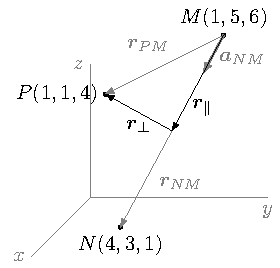
\includegraphics{figVectorExampleOrthognalVectorsHaveZeroDotProdcut}
\caption{متوازی اور عمودی اجزاء۔}
\label{شکل_سمتیہ_مثال_عمودی_سمتیات_کا_نقطہ_ضرب_صفر}
\end{figure}

حل:\عددیء{M} سے \عددیء{N} تک سمتیہ \عددیء{\kvec{r}_{NM}=3\ax-2\ay-5\az} ہے جس کا طول \عددیء{\abs{\kvec{r}_{NM}}=\sqrt{38}} ہے۔یوں اس سمت میں اکائی سمتیہ \عددیء{\kvec{a}_{NM}=\tfrac{3\ax-2\ay-5\az}{\sqrt{38}}} ہو گا۔ اسی طرح \عددیء{M} سے \عددیء{P} تک سمتیہ \عددیء{\kvec{r}_{PM}=-4\ay-2\az} ہے۔\عددیء{\kvec{a}_{NM}} کی سمت میں \عددیء{\kvec{r}_{PM}} کا طول
\begin{align*}
r_{\parallel}=\kvec{r}_{PM} \cdot \kvec{a}_{NM}&=(-4\ay-2\az) \cdot \left(\frac{3\ax-2\ay-5\az}{\sqrt{38}}\right) \\
&=\frac{0+8+10}{\sqrt{38}}=\frac{18}{\sqrt{38}}
\end{align*}
ہے یوں \عددیء{\kvec{a}_{NM}} سمت میں \عددیء{\kvec{r}_{PM}} کا سمتی جزو
\begin{align*}
\kvec{r}_{\parallel}=r_{\parallel} \kvec{a}_{NM}=\frac{18}{38} (3\ax-2\ay-5\az)
\end{align*}
ہے۔\عددیء{\kvec{r}_{PM}} سے \عددیء{\kvec{r}_{\parallel}} منفی کرنے سے لکیر سے \عددیء{P} تک عمودی سمتیہ \عددیء{\kvec{r}_\perp} حاصل ہوتا ہے
\begin{align*}
\kvec{r}_{\perp}=\kvec{r}_{PM}-\kvec{r}_{\parallel}&=(-4\ay-2\az)-\frac{18}{38} (3\ax-2\ay-5\az)\\
&=\frac{-27\ax-58\ay+7\az}{19}
\end{align*}
جس کا طول \عددیء{\tfrac{\sqrt{27^2+58^2+7^2}}{19}=3.3873} ہے۔یوں \عددیء{P} کا لکیر سے عمودی فاصلہ \عددیء{3.3873} ہے۔

\عددیء{\kvec{r}_{\parallel}} اور \عددیء{\kvec{r}_\perp} آپس میں عمودی ہیں لہٰذا ان  کا نقطہ ضرب
\begin{align*}
\kvec{r}_\parallel \cdot \kvec{r}_\perp&=\frac{18}{38} (3\ax-2\ay-5\az) \cdot \left(\frac{-27\ax-58\ay+7\az}{19}\right)=\frac{18}{722}(-81+116-35)=0
\end{align*}
صفر کے برابر ہے۔
\انتہا{مثال}
%===================

شکل \حوالہ{شکل_سمتیہ_مثال_عمودی_سمتیات_کا_نقطہ_ضرب_صفر} میں اگر \عددیء{M} پر \عددیء{\kvec{r}_{NM}} کی دُم رکھی جائے تب  \عددیء{\kvec{r}_{NM}} کی نوک \عددیء{N} کا مقام تعین کرتا ہے۔عموماً کسی بھی نقطے کا مقام محدد کے مرکز \عددیء{(0,0,0)} کی نسبت سے طے کیا جاتا ہے۔ایسا سمتیہ جس کی دُم مرکز پر رکھتے ہوئے اس کی نوک نقطے کا مقام طے کرے  \اصطلاح{مقام تعین کنندہ} سمتیہ\فرہنگ{مقام تعین کنندہ!سمتیہ}\حاشیہب{displacement vector}\فرہنگ{displacement vector} کہلاتا ہے۔اگر تعین کنندہ سمتیہ کو مرکز سے ہٹایا جائے تب ظاہر ہے اس کی نوک اصل مقام طے کرنے سے قاصر ہو گی۔
%=======================================
\ابتدا{مثال}
شکل \حوالہ{شکل_سمتیہ_مثال_عمودی_سمتیات_کا_نقطہ_ضرب_صفر} میں \عددیء{M} سے شروع ہوتے اور  \عددیء{N} جانب بڑھتی سیدھی لکیر پر کسی بھی نقطے کا مقام تعین کرتے تعین کنندہ سمتیہ حاصل کریں۔

حل:مرکز \عددیء{(0,0,0)} سے  نقطہ \عددیء{M} تک کا سمتیہ \عددیء{\kvec{r}_M=1\ax+5\ay+6\az} ہے جبکہ \عددیء{M} سے \عددیء{N} جانب اکائی سمتیہ \عددیء{\kvec{a}_{NM}} گزشتہ مثال میں حاصل کیا گیا۔اکائی سمتیہ \عددیء{\kvec{a}_{NM}} کی سمت میں  \عددیء{M} سے \عددیء{s} فاصلے پر نقطہ \عددیء{Q} تک کا سمتیہ \عددیء{s\kvec{a}_{NM}} ہے۔یوں مرکز سے  \عددیء{Q} تک سمتیہ \عددیء{\kvec{r}_Q=\kvec{r}_M+s\kvec{a}_{NM}} ہو گا۔
\begin{align*}
\kvec{r}_Q=(1\ax+5\ay+6\az) +s \left(\frac{3\ax-2\ay-5\az}{\sqrt{38}}\right)
\end{align*}   
اس مساوات میں \عددیء{s} متغیرہ ہے جسے تبدیل کرتے ہوئے سیدھی لکیر پر کسی بھی نقطہ \عددیء{Q} تک پہنچا جا سکتا ہے۔
\انتہا{مثال}
%==========================
\ابتدا{مثال}
\عددیء{z=z_0} پر \عددیء{1\az} کے عمودی سیدھی سطح کی مساوات حاصل کریں جہاں \عددیء{z_0} مستقل ہے۔ 

حل:نقطہ \عددیء{N_1(0,0,z_0)} سے کسی بھی نقطہ \عددیء{N_2(x,y,z)} تک کا سمتیہ \عددیء{\kvec{r}_{21}=x\ax+y\ay+(z-z_0)\az} ہے۔سطح پر کسی بھی سمتیہ اور سطح کے عمودی سمتیہ آپس میں نوے درجے زاویہ پر پائے جاتے ہیں لہٰذا ان کا غیر سمتی ضرب صفر کے برابر ہو گا۔یوں اگر \عددیء{N_2} اسی عمودی سطح پر پایا جائے تب
\begin{align*}
1\az \cdot [x\ax+y\ay+(z-z_0)\az]=z-z_0=0
\end{align*}
ہو گا جس سے اس سطح کی مساوات \عددیء{z=z_0} حاصل ہوتی ہے۔

اس قیمت کو \عددیء{\kvec{r}_{21}} میں پُر کرتے ہوئے \عددیء{\kvec{r}_{21}=x\ax+y\ay} حاصل ہوتا ہے جہاں \عددیء{x} اور \عددیء{y} آزاد متغیرات ہیں۔چونکہ مرکز سے \عددیء{N_1} کا تعین کنندہ سمتیہ \عددیء{\kvec{r}_{10}=z_0\az} ہے لہٰذا \عددیء{z=z_0} سطح پر کسی بھی نقطہ \عددیء{N_2} کا تعین کنندہ سمتیہ یعنی سطح کی سمتی مساوات  \عددیء{\kvec{r}_{20}=x\ax+y\ay+z_0\az} ہو گی۔
\انتہا{مثال}
%==========
\ابتدا{مشق}
مرکز سے \عددیء{(2,1,3)} تک کی سمتیہ ایک سیدھی سطح کی عمودی سمتیہ ہے۔اس سطح کی  مساوات حاصل کریں۔

جواب:\عددیء{2x+y+3z=14}
\انتہا{مشق}
%============
\حصہ{سمتی ضرب یا صلیبی ضرب}

دو سمتیات \عددیء{\kvec{A}} اور \عددیء{\kvec{B}} کے \اصطلاح{سمتی ضرب}\فرہنگ{سمتی ضرب}\فرہنگ{صلیبی ضرب}\حاشیہب{vector product}\فرہنگ{vector product} کا حاصل جواب سمتیہ ہوتا ہے جس کا طول \عددیء{\kvec{A}} کی مقدار ضربِ  \عددیء{\kvec{B}} کی مقدار ضربِ سمتیوں کے مابین چھوٹے زاویے کے سائن کے برابر ہے۔حاصل سمتیہ \عددیء{\kvec{A}} اور \عددیء{\kvec{B}} سمتیات کی عمودی سمت  میں ہوتا ہے جسے اکائی عمودی سمتیہ \عددیء{\kvec{a}_N} سے ظاہر کیا جائیگا۔
\begin{align}\label{مساوات_سمتیہ_سمتی_ضرب}
\kvec{A} \times \kvec{B}=\abs{\kvec{A}} \abs{\kvec{B}} \sin \theta_{AB} \kvec{a}_N
\end{align}
جس سیدھی سطح پر \عددیء{\kvec{A}} اور \عددیء{\kvec{B}} دونوں پائے جائیں، \عددیء{\kvec{a}_N} اس سطح کے دو عمودی سمتیات میں سے ایک ہے۔\عددیء{\kvec{a}_N} کو \اصطلاح{دائیں ہاتھ کے قانون}\فرہنگ{دائیں ہاتھ!قانون}\حاشیہب{right hand rule}\فرہنگ{right hand rule} سے یوں حاصل کیا جا سکتا ہے۔

\ابتدا{قانون}\شناخت{قانون_سمتیہ_دائیں_ہاتھ_قانون}
دائیں ہاتھ کی ہتھیلی  سیدھی اور انگوٹھے کو بقایا چار انگلیوں کے عمود میں رکھتے ہوئے پہلی انگلی کو \عددیء{\kvec{A}} اور  دوسری انگلی کو \عددیء{\kvec{B}} کی سمت میں رکھیں۔اس صورت میں انگوٹھا \عددیء{\kvec{a}_N} کی سمت میں ہو گا۔  
\انتہا{قانون}

اگر دونوں سمتیات کی دُم ایک ہی جگہ پر نہ ہو تب ان کے مابین زاویہ دریافت کرنے کی  خاطر سمتیوں کی سمت تبدیل کئے بغیر انہیں ایک نقطے پر منتقل کیا جا سکتا ہے۔سمتی ضرب کو سمتیوں کے درمیان صلیبی نشان \عددیء{\times} سے ظاہر کیا جاتا ہے۔اسی وجہ سے اسے \اصطلاح{صلیبی ضرب}\حاشیہب{cross product}\فرہنگ{cross product} بھی کہا جاتا ہے اور \عددیء{\kvec{A} \times \kvec{B}} کو "\عددیء{\kvec{A}} صلیب \عددیء{\kvec{B}}" پڑھا جاتا ہے۔سمتی ضرب میں سمتیوں کی ترتیب نہایت اہم ہے اور انہیں الٹانے سے حاصل جواب کی سمت الٹی ہو جاتی ہے۔
\begin{align}\label{مساوات_سمتیہ_صلیبی_ضرب_ترتیب_الٹاتے_منفی_سمت}
\kvec{A} \times \kvec{B}=- \kvec{B} \times \kvec{A}
\end{align}

اکائی سمتیات \عددیء{\ax} اور \عددیء{\ay} کے مابین نوے درجے کا زاویہ ہے  اور \عددیء{\sin 90\degree=1} کے برابر ہے جبکہ دائیں ہاتھ کے قانون سے ان کے صلیبی ضرب کی سمت \عددیء{\az} حاصل ہوتی ہے۔یوں \عددیء{\ax \times \ay=\az} کے برابر ہے۔اسی طرح \عددیء{\ay \times \az=\ax} اور \عددیء{\az \times \ax=\ay} کے برابر حاصل ہوتے ہیں۔مساوات \حوالہ{مساوات_سمتیہ_صلیبی_ضرب_ترتیب_الٹاتے_منفی_سمت} کے تحت یوں \عددیء{\ay \times \ax=-\az}، \عددیء{\az \times \ay=-\ax} اور \عددیء{\ax \times \az=-\ay} لکھے جا سکتے ہیں۔دو متوازی سمتیوں کے درمیان صفر درجے کا زاویہ ہوتا ہے اور \عددیء{\sin 0 =0} کے برابر ہے لہٰذا \عددیء{\ax \times \ax=0} کے برابر ہے۔اسی طرح \عددیء{\ay \times \ay=0} اور \عددیء{\az \times \az=0} کے برابر ہیں۔ان تمام جوابات کو ایک جگہ لکھتے ہیں۔
\begin{gather}
\begin{aligned}\label{مساوات_سمتیہ_کارتیسی_اکائی_سمتیات_صلیبی_ضرب}
\ax \times \ay &=\az & \ay \times \az&=\ax & \az \times \ax&=\ay\\
\ax \times \ax&=0 & \ay \times \ay&=0 & \az \times \az&=0
\end{aligned}
\end{gather}
%=================

یہی جوابات شکل \حوالہ{شکل_سمتیہ_صلیبی_ضرب_مثبت_دائرہ} کی مدد سے حاصل کئے جا سکتے ہیں۔اس شکل میں گھڑی کی الٹ سمت مثبت سمت ہے۔یوں اگر \عددیء{\ax \times \ay} حاصل کرنا ہو تو شکل میں \عددیء{\ax} سے شروع ہو کر \عددیء{\ay} کی جانب کم راستے پر چلتے ہوئے  \عددیء{\az} حاصل ہوتا ہے۔ساتھ ہی ساتھ چونکہ \عددیء{\ax} سے \عددیء{\ay} جانے کی خاطر  مثبت راستہ اختیار کیا گیا لہٰذا جواب مثبت یعنی \عددیء{+\az} ہو گا۔اس کے برعکس \عددیء{\az \times \ay} حاصل کرنے کی خاطر \عددیء{\az} سے \عددیء{\ay} جانب کم راستے پر چلتے ہوئے \عددیء{\ax} حاصل ہوتا ہے البتہ یہ راستہ گھڑی کے الٹ سمت یعنی منفی سمت میں ہے لہٰذا جواب \عددیء{-\ax} ہو گا۔ 
\begin{figure}
\centering
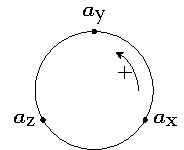
\includegraphics{figVectorCartesianRightHandCircle}
\caption{صلیبی ضرب کا حصول۔}
\label{شکل_سمتیہ_صلیبی_ضرب_مثبت_دائرہ}
\end{figure}

مساوات \حوالہ{مساوات_سمتیہ_کارتیسی_اکائی_سمتیات_صلیبی_ضرب} کی  مدد سے \عددیء{\kvec{A}=A_x\ax+A_y\ay+A_z\az} اور \عددیء{\kvec{B}=B_x\ax+B_y\ay+B_z\az} کی صلیبی ضرب
\begin{align*}
\kvec{A} \times \kvec{B}&=(A_x\ax+A_y\ay+A_z\az) \times (B_x\ax+B_y\ay+B_z\az)\\
&=A_x B_x \ax \times \ax+A_x B_y \ax \times \ay+A_x B_z \ax \times \az\\
& \quad \quad +A_y B_x \ay \times \ax+A_y B_y \ay \times \ay+A_y B_z \ay \times \az \\
&\quad \quad +A_z B_x \az \times \ax+A_z B_y \az \times \ay+A_z B_z \az \times \az
\end{align*}
کو
\begin{align}
\kvec{A} \times \kvec{B}=(A_y B_z-A_z B_y)\ax+(A_z B_x-A_x B_z)\ay+(A_x B_y-A_y B_x)\az
\end{align}
لکھا جا سکتا ہے۔اس جواب کو قالب کے حتمی قیمت کی شکل میں یوں لکھا جا سکتا ہے۔
\begin{align}
\kvec{A} \times \kvec{B}=\begin{vmatrix}
\ax & \ay & \az\\
A_x & A_y & A_z\\
B_x & B_y & B_z
\end{vmatrix}
\end{align}
یوں اگر \عددیء{\kvec{A}=2\ax-3\ay+1\az} اور \عددیء{\kvec{B}=6\ax+5\ay-4\az} ہوں تب
\begin{align*}
\kvec{A} \times \kvec{B}&=\begin{vmatrix*}[r]
\ax & \ay & \az\\
2 & -3 & 1\\
6 & 5 & -4
\end{vmatrix*}\\
&=[(-3)(-4)-(1)(5)]\ax-[(2)(-4)-(1)(6)]\ay+[(2)(5)-(-3)(6)]\az\\
&=7\ax+14\ay+18\az
\end{align*}
ہو گا۔
%===========
\ابتدا{مثال}
\عددیء{N_1(2,3,1)}، \عددیء{N_2(1,6,5)} اور \عددیء{N_3(-2,-3,2)} سیدھی سطح پر پائے جاتے ہیں۔اس سطح کی مساوات حاصل کریں۔

حل:
\begin{align*}
\kvec{r}_{21}&=(1-2)\ax+(6-3)\ay+(5-1)\az=-1\ax+3\ay+4\az\\
\kvec{r}_{31}&=(-2-2)\ax+(-3-3)\ay+(2-1)\az=-4\ax-6\ay+1\az
\end{align*}
کے سمتی ضرب سے ان کا عمودی سمتیہ حاصل ہو گا۔
\begin{align*}
\kvec{r}_N&=(-1\ax+3\ay+4\az) \times (-4\ax-6\ay+1\az)\\
&=6\az+1\ay+12\az+3\ax-16\ay+24\ax\\
&=27\ax-15\ay+18\az
\end{align*}
سطح پر دئے گئے تین نقطوں سے سطح پر کسی بھی نقطہ \عددیء{N_4(x,y,z)} تک کا سمتیہ اس عمودی سمتیہ کے نوے درجے زاویہ پر ہو گا اور یوں ان کا غیر سمتی ضرب صفر کے برابر ہو گا۔\عددیء{N_1} سے \عددیء{N_4} تک سمتیہ \عددیء{\kvec{r}_{41}=(x-2)\ax+(y-3)\ay+(z-1)\az} کے استعمال سے
\begin{align*}
\kvec{r}_{41} \cdot \kvec{r}_{N}=[(x-2)\ax+(y-3)\ay+(z-1)\az] \cdot (27\ax-15\ay+18\az)=0
\end{align*}
لکھ کر
\begin{align*}
27(x-2)-15(y-3)+18(z-1)=0
\end{align*}
سے
\begin{align*}
27x-15y+18z=27
\end{align*}
سیدھی سطح کی مساوات حاصل ہوتی ہے۔ایسی مساوات میں \عددیء{x}، \عددیء{y} اور \عددیء{z} کے مخفف عمودی سمتیہ میں \عددیء{\ax}، \عددیء{\ay} اور \عددیء{\az} کے مخفف \عددیء{27}، \عددیء{-15} اور \عددیء{18} ہوتے ہیں۔

سطح کی مساوات سے \عددیء{z=\tfrac{9-9x+5y}{6}} لکھا جا سکتا ہے۔سطح پر \عددیء{N_4} کی تعین کنندہ مساوات \عددیء{\kvec{r}=x\ax+y\ay+z\az} میں \عددیء{z} کی قیمت پُر کرتے ہوئے  سطح کی سمتی مساوات 
\begin{align*}
\kvec{r}=x\ax+y\ay+\left(\frac{9-9x+5y}{6}\right)\az
\end{align*}
لکھی جا سکتی ہے جہاں \عددیء{x} اور \عددیء{y} آزاد متغیرات ہیں جبکہ \عددیء{z} کو بطور تابع متغیرہ لکھا گیا ہے۔
\انتہا{مثال}
%=========

\ابتدا{مشق}
\عددیء{\kvec{A}=1\ax+3\ay-2\az} اور \عددیء{\kvec{B}=5\ax-2\ay-3\az} کی صورت میں \عددیء{\kvec{A} \times \kvec{B}}، \عددیء{\kvec{B}\times \kvec{A}}، \عددیء{\kvec{A} \times \kvec{A}}، \عددیء{\kvec{a}_B \times \kvec{A}} اور \عددیء{\az \times (\ay \times \kvec{B})} حاصل کریں۔ 
\انتہا{مشق}
%========================

خلاء میں کسی بھی نقطے کا مقام کارتیسی محدد کے علاوہ دیگر طرز کے محدد سے بھی تعین کیا جا سکتا ہے۔ماہرین طبیعیات  تقریباً ایک درجن اقسام کے محددی نظام استعمال کرتے ہیں۔ہم اس کتاب میں کارتیسی نظام کے علاوہ دو مزید اقسام کے محددی نظام استعمال کریں گے۔آئیں انہیں پر غور کریں۔ 

\حصہ{گول نلکی محدد}
کارتیسی نظام میں کسی بھی نقطے کا مقام مرکز سے \عددیء{x}، \عددیء{y} اور \عددیء{z} سمتوں میں فاصلوں سے طے کیا جاتا ہے۔آئیں اب ایسا نظام دیکھیں جس میں ایک عدد زاویہ اور دو عدد فاصلے استعمال کرتے ہوئے کسی بھی نقطے کا مقام طے ہو۔
 \begin{figure}
\centering
\begin{subfigure}{0.5\textwidth}
\centering
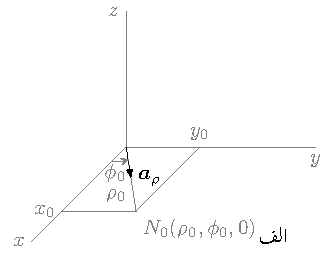
\includegraphics{figVector2and3Dcylindrical}
\end{subfigure}%
%
\begin{subfigure}{0.5\textwidth}
\centering
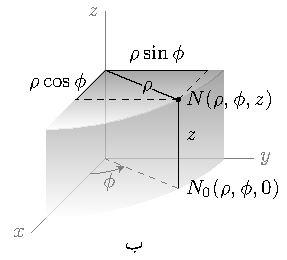
\includegraphics{figVectorCylindricalToCartesian}
\end{subfigure}%
\caption{نلکی محدد}
\label{شکل_سمتیہ_نلکی_محدد}
\end{figure}

شکل \حوالہ{شکل_سمتیہ_نلکی_محدد}-الف میں \عددیء{z=0} سطح پر نقطہ \عددیء{N_0} دکھایا گیا ہے جسے کارتیسی محدد میں \عددیء{N_0(x_0,y_0,0)} لکھا جائے گا۔اگر مرکز سے \عددیء{N_0} تک سیدھی لکیر کی لمبائی \عددیء{\rho_0} اور \عددیء{x} محدد سے اس لکیر کا زاویہ \عددیء{\phi_0} ہو تب اسی نقطے
 کو \اصطلاح{گول نلکی محدد}\فرہنگ{نلکی!محدد}\حاشیہب{cylindrical coordinate system}\فرہنگ{cylindrical!coordinates} کے نظام میں \عددیء{N_0(\rho_0,\phi_0,0)} لکھا جاتا ہے۔اس کتاب میں گول نلکی محدد کا نام چھوٹا کر کے اسے \اصطلاح{نلکی محدد} پکارا جائے گا۔ اگر \عددیء{z=0} سطح پر مرکز سے نقطے کی جانب اکائی سمتیہ \عددیء{\arho} ہو تب مرکز سے نقطے تک سمتیہ کو
\begin{align}
\kvec{\rho}=\rho_0 \arho \quad \quad (\phi=\phi_0, \quad   z=0 )
\end{align}
   لکھا جا سکتا ہے۔نلکی  اور کارتیسی نظام میں  \عددیء{z} محدد یکساں ہیں۔

شکل \حوالہ{شکل_سمتیہ_نلکی_محدد}-الف یا شکل-ب سے کارتیسی اور نلکی محدد کے تعلق اخذ کئے جا سکتے ہیں۔یوں نلکی محدد کے متغیرات \عددیء{(\rho,\phi,z)} سے کارتیسی متغیرات \عددیء{(x,y,z)} یوں حاصل ہوتے ہیں۔
\begin{gather}
\begin{aligned}
x&=\rho \cos \phi\\
y&=\rho \sin \phi\\
z&=z
\end{aligned}
\end{gather}
اسی طرح \عددیء{(x,y,z)} سے  \عددیء{(\rho,\phi,z)} یوں حاصل کئے جاتے ہیں۔
\begin{gather}
\begin{aligned}
\rho&=\sqrt{x^2+y^2} \quad \quad (\rho \ge 0)\\
\phi&=\tan^{-1} \frac{y}{x}\\
z&=z
\end{aligned}
\end{gather}
%
\begin{figure}
\centering
\begin{subfigure}{0.5\textwidth}
\centering
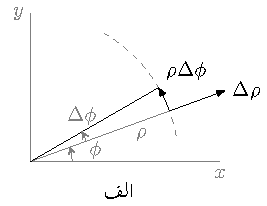
\includegraphics{figVectorCylindricalRadiusAngle}
\end{subfigure}%
%
\begin{subfigure}{0.5\textwidth}
\centering
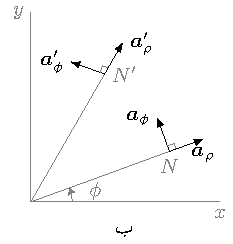
\includegraphics{figVectorCylindricalUnitVectors}
\end{subfigure}%
\caption{نلکی محدد میں متغیرات کے تبدیلی سے فاصلے کا حصول اور اکائی سمتیات۔}
\label{شکل_سمتیہ_نلکی_تبدیلی_متغیرات}
\end{figure}
مندرجہ بالا مساوات میں رداس کی صرف مثبت قیمت لی گئی۔ہم  رداس کی قیمت مثبت ہی لیتے ہیں۔

شکل \حوالہ{شکل_سمتیہ_نلکی_تبدیلی_متغیرات}-الف میں \عددیء{\phi} زاویہ پر \عددیء{\rho} رداس کا ہلکی سیاہی میں دکھایا سمتیہ نقطہ \عددیء{N} ہے۔
اس شکل میں \عددیء{\phi} اور \عددیء{z} تبدیل کئے بغیر \عددیء{\rho} کو \عددیء{\Delta \rho} بڑھتا دکھایا گیا ہے۔اس صورت میں سمتیہ کی نوک \عددیء{\Delta \rho} فاصلہ طے کرتی ہے۔نقطہ \عددیء{N} سے \عددیء{\Delta \rho} کی سمت میں اکائی سمتیہ جسے \عددیء{\arho} لکھا جاتا ہے، نلکی محدد کی  بنیادی اکائی سمتیہ ہے۔اس سمتیہ کو شکل \حوالہ{شکل_سمتیہ_نلکی_تبدیلی_متغیرات}-ب میں دکھایا گیا ہے۔

شکل \حوالہ{شکل_سمتیہ_نلکی_تبدیلی_متغیرات}-الف میں   \عددیء{\rho} اور \عددیء{z} تبدیل کئے بغیر \عددیء{\phi} کو \عددیء{\Delta \phi} بڑھا کر اسی سمتیہ کو گاڑھی سیاہی میں دوبارہ دکھایا گیا ہے۔آپ دیکھ سکتے ہیں کہ  سمتیہ کی نوک نے \عددیء{\rho} رداس کے گول دائرے پر حرکت کرتے ہوئے  \عددیء{\rho \Delta \phi} فاصلہ طے کیا۔یوں اگر زاویہ کو \عددیء{0} تا \عددیء{2\pi} ریڈیئن تبدیل کیا جائے  تو سمتیہ کی نوک گول دائرے پر ایک مکمل چکر کاٹے گی۔جیسے جیسے \عددیء{\Delta \phi} کو کم سے کم کیا جائے ویسے ویسے  \عددیء{\rho \Delta \phi}  گول دائرے کے مماس کی صورت اختیار کرے گی حتٰی کہ \عددیء{\dif \phi} کی صورت میں \عددیء{\rho \dif \phi} گول دائرے کا مماس ہو گا۔نقطہ \عددیء{N} پر بڑھتے \عددیء{\phi} جانب مماس کی سمت میں اکائی سمتیہ کو \عددیء{\aphi} لکھا جاتا ہے۔ اس سمتیہ کو شکل \حوالہ{شکل_سمتیہ_نلکی_تبدیلی_متغیرات}-ب میں دکھایا گیا ہے۔

اسی طرح اگر نقطہ \عددیء{N} پر صرف \عددیء{z} کو \عددیء{\Delta z} تبدیل کیا جائے تب سمتیہ کی نوک \عددیء{\Delta z} فاصلہ طے کرے گی۔ \عددیء{\Delta z} کی سمت میں اکائی سمتیہ جسے \عددیء{\az} لکھا جاتا ہے، نلکی محدد کی تیسری اور آخری بنیادی اکائی سمتیہ ہے۔نلکی محدد کے تین اکائی سمتیات \عددیء{\arho}، \عددیء{\aphi} اور \عددیء{\az} مل کر دائیں ہاتھ کا عمودی  نظام دیتے ہیں۔نقطہ \عددیء{(\rho_1,\phi_1,z_1)} پر نلکی محدد کے اکائی سمتیات کو شکل \حوالہ{شکل_سمتیہ_نلکی_اکائی_سمتیات_عمومی} میں دکھایا گیا ہے۔\عددیء{\arho} گول سطح \عددیء{\rho=\rho_1} کے عمودی ہے۔یہ \عددیء{\phi=\phi_1} اور \عددیء{z=z_1} سطحوں پر پایا جاتا ہے۔اسی طرح \عددیء{\aphi} سیدھی سطح  \عددیء{\phi=\phi_1} کے عمودی ہے۔ یہ \عددیء{z=z_1} سطح پر پایا جاتا ہے اور \عددیء{\rho=\rho_1} نلکی سطح کا مماس ہے۔\عددیء{\az} اکائی سمتیہ \عددیء{z=z_1} سطح کے عمودی ہے۔یہ \عددیء{\rho=\rho_1} اور \عددیء{\phi=\phi_1} سطحوں پر پایا جاتا ہے۔ 
\begin{figure}
\centering
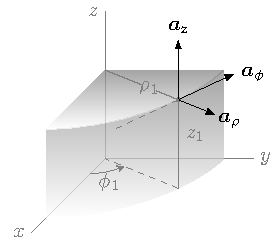
\includegraphics{figVectorCylindricalUnitVectorDirectionsInThreeD}
\caption{نلکی محدد کے اکائی سمتیات۔}
\label{شکل_سمتیہ_نلکی_اکائی_سمتیات_عمومی}
\end{figure}

دائیں ہاتھ کے عمودی نظام میں سمتی ضرب کا حاصل جواب صفحہ \حوالہصفحہ{قانون_سمتیہ_دائیں_ہاتھ_قانون} پر دئے گئے دائیں ہاتھ کے قانون کی مدد سے حاصل کیا جاتا ہے ۔ یوں
\begin{align}
\arho \times \aphi=\az, \quad \aphi \times \az=\arho, \quad \az \times \arho=\aphi
\end{align}
لکھا جا سکتا ہے۔یہی جوابات شکل \حوالہ{شکل_سمتیہ_نلکی_صلیبی_ضرب_مثبت_دائرہ} سے بھی اخذ کئے جا سکتے ہیں۔
\begin{figure}
\centering
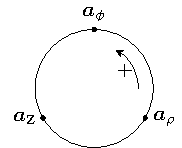
\includegraphics{figVectorCylindricalRightHandCircle}
\caption{صلیبی ضرب کی حاصل اکائی سمتیہ۔}
\label{شکل_سمتیہ_نلکی_صلیبی_ضرب_مثبت_دائرہ}
\end{figure}

کسی سمتیہ کا خود سمتی ضرب صفر کے برابر ہوتا ہے لہٰذا
\begin{align}
\arho \times \arho=0, \quad \aphi \times \aphi =0, \quad \az \times \az=0
\end{align}
لکھا جا سکتا ہے جبکہ کسی بھی اکائی سمتیہ کا خود غیر سمتی ضرب ایک کے برابر ہوتا ہے لہٰذا 
\begin{align}
\arho \cdot \arho=1, \quad \aphi \cdot \aphi =1, \quad \az \cdot \az =1
\end{align}
لکھا جا سکتا ہے۔اسی طرح کسی بھی دو عمودی سمتیات  کا غیر سمتی ضرب صفر کے برابر ہوتا ہے یعنی
\begin{align}
\arho \cdot \aphi=0, \quad \aphi \cdot \az =0, \quad \az \cdot \arho =0
\end{align}

غیر سمتی ضرب کو  \اصطلاح{کرونیکر ڈیلٹا} کی مدد سے یوں لکھا جا سکتا ہے۔
\begin{align}
\kvec{a}_i \cdot \kvec{a}_j=\delta_{ij}
\end{align}
جہاں
\begin{align}
\delta_{ij}=
\begin{cases}
0 \quad  \quad  i\ne j \; \textup{ اگر}\\
1 \quad \quad i=j \; \textup{ اگر}
\end{cases}
\end{align}
کے برابر ہے۔

آپ دیکھتے ہیں کہ کسی بھی نقطہ \عددیء{N(\rho,\phi,z)} پر  اکائی سمتیات حاصل کرنے کی خاطر محدد کے متغیرات \عددیء{\rho}، \عددیء{\phi} اور \عددیء{z} کو  باری باری انتہائی کم بڑھایا جاتا ہے۔جس سمت میں نقطہ حرکت کرے، اسی سمت میں اکائی سمتیہ ہو گی۔شکل \حوالہ{شکل_سمتیہ_نلکی_تبدیلی_متغیرات}-ب میں دو مختلف نقاط \عددیء{N} اور \عددیء{N'} پر نلکی محدد کے عمودی اکائی سمتیات دکھائے گئے ہیں۔آپ دیکھ سکتے ہیں کہ نلکی محدد کے عمودی اکائی سمتیات کی سمت کا دارومدار اس نقطے پر ہے جہاں انہیں حاصل کیا جائے۔آپ جانتے ہیں کہ کارتیسی نظام میں نقطے کا مقام تبدیل کرنے سے کارتیسی اکائی سمتیات تبدیل نہیں ہوتے۔یوں نلکی محدد کے اکائی سمتیات اٹل نہیں ہیں۔یہ ایک انتہائی اہم حقیقت ہے جو تکمل لیتے وقت پیچیدگیاں پیدا کرتا ہے۔تکمل لیتے وقت کارتیسی اکائی سمتیات اٹل ہونے کی بنا پر تکمل کے باہر لے جائے جا سکتے ہیں جبکہ نلکی محدد کے  \عددیء{\arho} اور \عددیء{\aphi} اکائی سمتیات کو تکمل کے باہر نہیں لے جایا جا سکتا۔یاد رہے کہ کسی بھی نقطہ \عددیء{N} پر حاصل کئے گئے \عددیء{\arho}، \عددیء{\aphi} اور \عددیء{\az} آپس میں عمودی ہوں گے جبکہ کسی اور نقطہ \عددیء{N'} پر حاصل کئے گئے \عددیء{\arho'}، \عددیء{\aphi'} اور \عددیء{\az} آپس میں عمودی ہوں گے۔

\جزوحصہ{نلکی اکائی سمتیات کا کارتیسی اکائی سمتیات کے ساتھ غیر سمتی ضرب}
شکل \حوالہ{شکل_سمتیہ_نلکی_کارتیسی_اکائی_غیر_سمتی_ضرب}-الف میں نقطہ \عددیء{N} پر اکائی سمتیات \عددیء{\arho}، \عددیء{\ax} اور \عددیء{\ay} دکھائے گئے ہیں۔\عددیء{\arho} اور  \عددیء{\ax} کے مابین زاویہ \عددیء{\phi} ہے جبکہ اکائی سمتیات کی لمبائی ایک ہوتی ہے لہٰذا
\begin{align}
\arho \cdot \ax=(1)(1)(\cos \phi)=\cos \phi
\end{align}
ہے۔\عددیء{\arho} اور  \عددیء{\ay} کے مابین زاویہ \عددیء{(90^\circ-\phi)} ہے  لہٰذا
\begin{align}
\arho \cdot \ay=(1)(1)[\cos (90^\circ-\phi)]=\sin \phi
\end{align}
کے برابر ہے۔اس مساوات میں \عددیء{\cos(\alpha-\beta)=\cos \alpha \cos \beta+\sin \alpha \sin \beta} کو استعمال کرتے ہوئے \عددیء{\cos(90^\circ-\phi)=\sin \phi} لکھا گیا ہے۔شکل \حوالہ{شکل_سمتیہ_نلکی_کارتیسی_اکائی_غیر_سمتی_ضرب}-ب میں نقطہ \عددیء{N} پر اکائی سمتیات \عددیء{\aphi}، \عددیء{\ax} اور \عددیء{\ay} دکھائے گئے ہیں۔\عددیء{\aphi} اور  \عددیء{\ax} کے مابین زاویہ \عددیء{(90^\circ+\phi)} ہے  لہٰذا
\begin{align}
\aphi \cdot \ax=(1)(1)[\cos (90^\circ+\phi)]=-\sin \phi
\end{align}
ہے۔\عددیء{\aphi} اور  \عددیء{\ay} کے مابین زاویہ \عددیء{\phi} ہے  لہٰذا
\begin{align}
\aphi \cdot \ay=(1)(1)(\cos \phi)=\cos \phi
\end{align}
کے برابر ہے۔\عددیء{\az} کا \عددیء{\ax} اور \عددیء{\ay} کے ساتھ غیر سمتی ضرب صفر کے برابر ہے۔اس کی وجہ ان کے مابین نوے درجے کا زاویہ ہے۔ان تمام غیر سمتی ضرب کو جدول \حوالہ{جدول_سمتیہ_نلکی_کارتیسی_اکائی_غیر-سمتی_ضرب} میں یکجا کیا گیا ہے۔
\begin{figure}
\centering
\begin{subfigure}{0.5\textwidth}
\centering
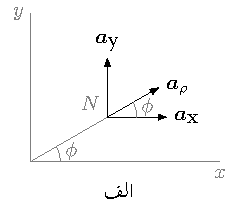
\includegraphics{figVectorCylindricalXandRhoDotProduct}
\end{subfigure}%
%
\begin{subfigure}{0.5\textwidth}
\centering
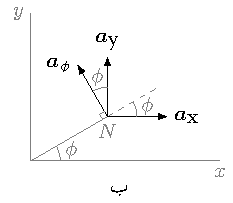
\includegraphics{figVectorCylindricalXandPhiDotProduct}
\end{subfigure}%
\caption{نلکی اکائی سمتیات کا کارتیسی اکائی سمتیات کے ساتھ غیر سمتی ضرب۔}
\label{شکل_سمتیہ_نلکی_کارتیسی_اکائی_غیر_سمتی_ضرب}
\end{figure}%
%
%
\begin{table}
\caption{نلکی اکائی سمتیات کا کارتیسی اکائی سمتیات کے ساتھ غیر سمتی ضرب۔}
\centering
\begin{tabular}{l | r r r}
 & $\ax$ & $\ay$ & $\az$ \\
\hline
$\arho$ & $\cos \phi$ & $\sin \phi $& $0$\\
$\aphi$ &$-\sin \phi$ &$ \cos \phi$ &$ 0$\\
$\az$ & $0$ &$ 0$ &$1$
\end{tabular}
\label{جدول_سمتیہ_نلکی_کارتیسی_اکائی_غیر-سمتی_ضرب}
\end{table}
%
\begin{figure}
\centering
\begin{subfigure}{0.5\textwidth}
\centering
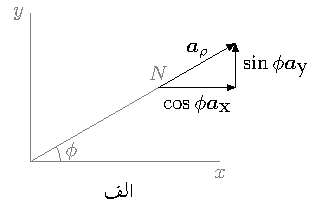
\includegraphics{figVectorCylindricalRhoToCartesianConversion}
\end{subfigure}%
%
\begin{subfigure}{0.5\textwidth}
\centering
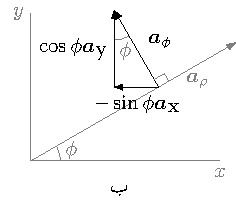
\includegraphics{figVectorCylindricalPhiToCartesianConversion}
\end{subfigure}%
\caption{\عددیء{\arho} اور \عددیء{\aphi} کا کارتیسی نظام میں تبادلہ۔}
\label{شکل_سمتیہ_کارتیسی_نظام_میں_نلکی_رداس_اکائی}
\end{figure}%

\جزوحصہ{نلکی اور کارتیسی اکائی سمتیات کا تعلق}
شکل \حوالہ{شکل_سمتیہ_کارتیسی_نظام_میں_نلکی_رداس_اکائی}-الف میں نقطہ \عددیء{N} پر اکائی سمتیہ \عددیء{\arho} دکھایا گیا ہے۔آپ دیکھ سکتے ہیں کہ کارتیسی محدد میں اسی اکائی سمتیہ کو دو عدد سمتیات کی مدد سے لکھا جا سکتا ہے۔\عددیء{\arho} کی لمبائی ایک کے برابر ہے۔یوں مسئلہ فیثاغورث کی مدد سے
\begin{gather}
\begin{aligned}\label{مساوات_سمتیہ_اکائی_رداس_کارتیسی_میں}
\arho&=\cos \phi \ax+\sin \phi \ay\\
&=\frac{x}{\sqrt{x^2+y^2}} \ax+\frac{y}{\sqrt{x^2+y^2}} \ay
\end{aligned}
\end{gather}
 لکھا جا سکتا ہے جہاں دوسرے قدم پر تمام نلکی محدد کے متغیرات کو کارتیسی متغیرات کی شکل میں لکھا گیا ہے۔شکل \حوالہ{شکل_سمتیہ_کارتیسی_نظام_میں_نلکی_رداس_اکائی}-ب میں نقطہ \عددیء{N} پر اکائی سمتیہ \عددیء{\aphi} دکھایا گیا ہے۔آپ دیکھ سکتے ہیں کہ کارتیسی محدد میں اسی اکائی سمتیہ کو دو عدد سمتیات کی مدد سے یوں  لکھا جا سکتا ہے
\begin{gather}
\begin{aligned}\label{مساوات_سمتیہ_اکائی_زاویہ_کارتیسی_میں}
\aphi&=-\sin \phi \ax+\cos \phi \ay\\
&=-\frac{y}{\sqrt{x^2+y^2}} \ax+\frac{x}{\sqrt{x^2+y^2}} \ay
\end{aligned}
\end{gather}
جہاں دوسرے قدم پر تمام نلکی محدد کے متغیرات کو کارتیسی متغیرات کی شکل میں لکھا گیا ہے۔
%
\begin{figure}
\centering
\begin{subfigure}{0.5\textwidth}
\centering
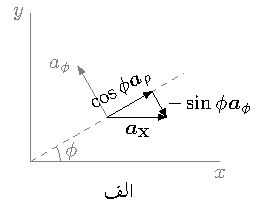
\includegraphics{figVectorCartesianXtoCylindricalConversion}
\end{subfigure}%
%
\begin{subfigure}{0.5\textwidth}
\centering
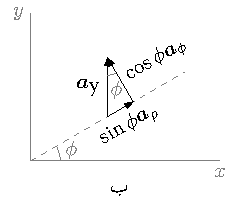
\includegraphics{figVectorCartesianYtoCylindricalConversion}
\end{subfigure}%
\caption{\عددیء{\ax} اور \عددیء{\ay} کا نلکی محدد میں تبادلہ۔}
\label{شکل_سمتیہ_نلکی_محدد_میں_کارتیسی_اکائی_سمتیات}
\end{figure}%

شکل \حوالہ{شکل_سمتیہ_نلکی_محدد_میں_کارتیسی_اکائی_سمتیات}-الف میں \عددیء{\ax} کا نلکی محدد میں تبادلہ دکھایا گیا ہے۔جس نقطے پر ایسا درکار ہو، اس نقطے پر \عددیء{\ax} کی دُم رکھیں۔مرکز سے نقطے تک نقطہ دار سیدھی لکیر کھینچتے ہوئے اسے مزید آگے بڑھائیں۔اس نقطے پر \عددیء{\arho} اسی لکیر کی سمت میں ہو گا جبکہ \عددیء{\aphi} لکیر کے ساتھ نوے درجے کا زاویہ بنائے گا۔شکل میں \عددیء{\aphi} دکھایا گیا ہے۔جیسا شکل میں دکھایا گیا ہے، \عددیء{\ax} کی نوک سے نقطہ دار لکیر پر عمود بنائیں۔صاف ظاہر ہے کہ \عددیء{\ax} کو دو عدد سمتیات کی مدد سے لکھا جا سکتا ہے۔ان میں سے ایک سمتیہ \عددیء{\arho} کی سمت میں اور دوسرا سمتیہ \عددیء{\aphi} کی الٹ جانب کو ہو گا۔یوں
\begin{align}\label{مساوات_سمتیہ_اکائی_ایکس_نلکی_میں}
\ax=\cos \phi \arho-\sin \phi \aphi
\end{align}
لکھا جا سکتا ہے۔شکل \حوالہ{شکل_سمتیہ_نلکی_محدد_میں_کارتیسی_اکائی_سمتیات}-ب میں \عددیء{\ay} کا نلکی محدد میں تبادلہ دکھایا گیا ہے۔یہاں نقطہ پر \عددیء{\ay} کی دُم رکھتے ہوئے اس کی نوک سے نقطہ دار لکیر پر عمود کھینچا گیا ہے۔یوں
\begin{align}\label{مساوات_سمتیہ_اکائی_وائے_نلکی_میں}
\ay=\sin \phi \arho+\cos \phi \aphi
\end{align}
لکھا جا سکتا ہے۔

آئیں مساوات \حوالہ{مساوات_سمتیہ_اکائی_رداس_کارتیسی_میں} تا مساوات \حوالہ{مساوات_سمتیہ_اکائی_وائے_نلکی_میں} کو جدول \حوالہ{جدول_سمتیہ_نلکی_کارتیسی_اکائی_غیر-سمتی_ضرب} کی مدد سے حاصل کریں۔کسی بھی سمتیہ \عددیء{\kvec{A}} کو کارتیسی یا نلکی محدد میں لکھا جا سکتا ہے۔یوں
\begin{gather}
\begin{aligned}\label{مساوات_سمتیہ_سمتیہ_نلکی_کارتیسی_اشکال}
\kvec{A}&=A_x \ax+A_y \ay+A_z\az\\
&=A_\rho \arho+A_\phi \aphi+A_z \az
\end{aligned}
\end{gather}
لکھا جا سکتا ہے۔ان میں پہلی مساوات کا باری باری \عددیء{\ax}، \عددیء{\ay} اور \عددیء{\az} کے ساتھ غیر سمتی ضرب لیتے ہوئے 
\begin{gather}
\begin{aligned}\label{مساوات_سمتیہ_کارتیسی_اجزاء}
\ax \cdot \kvec{A}&=A_x \ax \cdot \ax+A_y \ax \cdot \ay+A_z \ax \cdot \az=A_x\\
\ay \cdot \kvec{A}&=A_x \ay \cdot \ax+A_y \ay \cdot \ay+A_z \ay \cdot \az=A_y\\
\az \cdot \kvec{A}&=A_x \az \cdot \ax+A_y \az \cdot \ay+A_z \az \cdot \az=A_z
\end{aligned}
\end{gather}
حاصل ہوتے ہیں۔\عددیء{\kvec{A}} کو کارتیسی نظام میں لکھنے کی خاطر \عددیء{A_x}، \عددیء{A_y} اور \عددیء{A_z} درکار ہوتے ہیں جنہیں مندرجہ بالا مساوات سے حاصل کیا جا سکتا ہے۔اسی طرح مساوات \حوالہ{مساوات_سمتیہ_سمتیہ_نلکی_کارتیسی_اشکال} کے نچلے حصے کا باری باری \عددیء{\arho}، \عددیء{\aphi} اور \عددیء{\az} کے ساتھ غیر سمتی ضرب لیتے ہوئے
\begin{gather}
\begin{aligned}\label{مساوات_سمتیہ_نلکی_اجزاء}
\arho \cdot \kvec{A}&=A_\rho \arho \cdot \arho +A_\phi \arho \cdot \aphi +A_z \arho \cdot \az=A_\rho\\
\aphi \cdot \kvec{A}&=A_\rho \aphi \cdot \arho +A_\phi \aphi \cdot \aphi +A_z \aphi \cdot \az=A_\phi \\
\az \cdot \kvec{A}&=A_\rho \az \cdot \arho +A_\phi \az \cdot \aphi +A_z \az \cdot \az=A_z
\end{aligned}
\end{gather}
حاصل ہوتے ہیں۔یوں \عددیء{\kvec{A}} کو نلکی نظام میں لکھنے کی خاطر \عددیء{A_\rho}، \عددیء{A_\phi} اور \عددیء{A_z} کو مندرجہ بالا مساوات کی مدد سے حاصل کیا جا سکتا ہے۔

آئیں \عددیء{\arho} کو کارتیسی نظام میں لکھیں۔یوں \عددیء{\kvec{A}=\arho} کو  کارتیسی نظام میں لکھنا مطلوب ہے۔مساوات \حوالہ{مساوات_سمتیہ_کارتیسی_اجزاء} کے مطابق  \عددیء{A_x} حاصل کرنے کی خاطر \عددیء{\ax \cdot \kvec{A}} لینا ہو گا۔جدول \حوالہ{جدول_سمتیہ_نلکی_کارتیسی_اکائی_غیر-سمتی_ضرب} کے استعمال سے
\begin{align*}
A_x=\ax \cdot \kvec{A}=\ax \cdot \arho=\cos \phi
\end{align*}  
حاصل ہوتا ہے۔اسی طرح جدول کو استعمال کرتے ہوئے
\begin{align*}
A_y=\ay \cdot \kvec{A}=\ay \cdot \arho=\sin \phi
\end{align*}
اور 
\begin{align*}
A_z=\az \cdot \kvec{A}=\az \cdot \arho=0
\end{align*}
حاصل کرتے  ہیں۔یوں کارتیسی نظام میں \عددیء{\kvec{A}=A_x\ax+A_y\ay+A_z\az} لکھتے ہوئے
\begin{align*}
\arho = \cos \phi \ax +\sin \phi \ay
\end{align*}
لکھا جائے گا۔ یہی جواب مساوات \حوالہ{مساوات_سمتیہ_اکائی_رداس_کارتیسی_میں} میں بھی حاصل کیا گیا تھا۔

\عددیء{\aphi} کو بھی اسی طرح کارتیسی نظام میں لکھا جا سکتا ہے۔ایسا کرنے کی خاطر جدول \حوالہ{جدول_سمتیہ_نلکی_کارتیسی_اکائی_غیر-سمتی_ضرب} کی مدد سے  اس سمتیہ کا باری باری \عددیء{\ax}، \عددیء{\ay} اور \عددیء{\az} کے ساتھ غیر سمتی ضرب لیتے ہیں۔
\begin{align*}
A_x&=\ax \cdot \aphi=-\sin \phi\\
A_y&=\ay \cdot \aphi=\cos \phi\\
A_z&=\az \cdot \aphi=0
\end{align*}
یوں
\begin{align*}
\aphi=A_x \ax+A_y \ay+A_z \az = -\sin \phi \ax+\cos \phi \ay
\end{align*}
حاصل ہوتا ہے۔یہی جواب مساوات \حوالہ{مساوات_سمتیہ_اکائی_زاویہ_کارتیسی_میں} بھی دیتا ہے۔

آپ سے گزارش ہے کہ جدول \حوالہ{مساوات_سمتیہ_اکائی_زاویہ_کارتیسی_میں} کو یاد کرنے کی کوشش نہ کریں۔اپنے آپ میں یہ صلاحیت پیدا کریں کہ ان جوابات کو آپ جلد اخذ کر سکیں۔

\ابتدا{مشق}
\عددیء{\ax}، \عددیء{\ay} اور \عددیء{\az} کو جدول \حوالہ{جدول_سمتیہ_نلکی_کارتیسی_اکائی_غیر-سمتی_ضرب} کی مدد سے  نلکی محدد میں لکھیں۔
\انتہا{مشق}
%
\begin{figure}
\centering
\begin{subfigure}{0.5\textwidth}
\centering
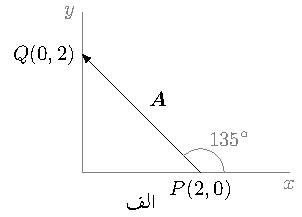
\includegraphics{figVectorVectorInCartesianAndCylindricalA}
\end{subfigure}%
%
\begin{subfigure}{0.5\textwidth}
\centering
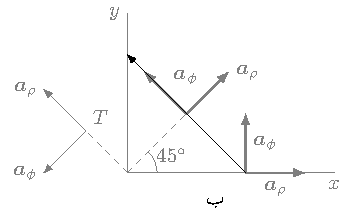
\includegraphics{figVectorVectorInCartesianAndCylindricalB}
\end{subfigure}%
\caption{کارتیسی اور نلکی محدد میں سمتیہ۔}
\label{شکل_سمتیہ_کارتیسی_نلکی_مساوات}
\end{figure}

شکل \حوالہ{شکل_سمتیہ_کارتیسی_نلکی_مساوات} میں \عددیء{P(2,0)} سے \عددیء{Q(0,2)} تک سمتیہ \عددیء{\kvec{A}} دکھایا گیا ہے۔کارتیسی نظام میں 
\begin{align}\label{مساوات_سمتیہ_کارتیسی_نظام_سمتیہ_مثال}
\kvec{A}&=-2\ax+2\ay
\end{align}
لکھا جا سکتا ہے۔اس سمتیہ کی حتمی قیمت
\begin{align*}
\abs{\kvec{A}}= \sqrt{\kvec{A} \cdot \kvec{A}}=\sqrt{(-2\ax+2\ay) \cdot (-2\ax+2\ay)}=\sqrt{8}
\end{align*}
ہے۔آئیں اسی سمتیہ کو نلکی محدد میں لکھیں۔ایسا کرنے کی خاطر \عددیء{A_\rho} اور \عددیء{A_\phi} درکار ہوں گے جنہیں حاصل کرنے کی خاطر جدول \حوالہ{جدول_سمتیہ_نلکی_کارتیسی_اکائی_غیر-سمتی_ضرب}  کی مدد سے \عددیء{\arho \cdot \kvec{A}} اور \عددیء{\aphi \cdot \kvec{A}} حاصل کرتے ہیں۔
\begin{align*}
A_\rho&=\arho \cdot (-2\ax+2\ay)=-2 \cos \phi +2 \sin \phi\\
A_\phi&=\aphi \cdot  (-2\ax+2\ay)=2 \sin \phi +2 \cos \phi
\end{align*}
یوں
\begin{align}\label{مساوات_سمتیہ_نلکی_نظام_سمتیہ_مثال}
\kvec{A}=2(- \cos \phi + \sin \phi) \arho +2( \sin \phi + \cos \phi)\aphi
\end{align}
لکھا جا سکتا ہے۔آئیں دیکھیں کہ اس کی حتمی قیمت کیا حاصل ہوتی ہے۔اکائی سمتیات کا غیر سمتی ضرب \عددیء{\arho \cdot \arho=1}، \عددیء{\aphi \cdot \aphi=1} اور \عددیء{\arho \cdot \aphi=0} استعمال کرتے ہوئے
\begin{align*}
\abs{\kvec{A}}&=\sqrt{\kvec{A} \cdot \kvec{A}}\\
&=\sqrt{2^2(- \cos \phi + \sin \phi)^2+2^2( \sin \phi + \cos \phi)^2 }\\
&=\sqrt{4(\cos^2 \phi +\sin^2 \phi -2 \cos \phi \sin \phi)+4(\cos^2 \phi +\sin^2 \phi +2 \cos \phi \sin \phi)}\\
&=\sqrt{8(\cos^2 \phi+\sin^2 \phi)}\\
&=\sqrt{8}
\end{align*}
حاصل ہوتا ہے جہاں آخری قدم پر \عددیء{\cos^2 \alpha+\sin^2 \alpha=1} کا استعمال کیا گیا ہے۔یقیناً سمتیہ کی حتمی قیمت محدد کے نظام پر منحصر نہیں۔

مساوات \حوالہ{مساوات_سمتیہ_کارتیسی_نظام_سمتیہ_مثال} اور مساوات \حوالہ{مساوات_سمتیہ_نلکی_نظام_سمتیہ_مثال} ایک ہی سمتیہ کو لکھنے کے دو طریقے ہیں۔یہاں کارتیسی نظام کا استعمال نہایت آسان ثابت ہوا۔ آگے چل کر آپ دیکھیں گے کہ کہیں مسئلوں میں نلکی محدد کا استعمال زیادہ آسان ہو گا۔آئیں مساوات \حوالہ{مساوات_سمتیہ_کارتیسی_نظام_سمتیہ_مثال} پر مزید غور کریں۔اس مساوات میں اکائی سمتیات از خود اٹل نہیں ہیں۔ان کی سمتوں کا دارومدار زاویہ \عددیء{\phi} پر ہے۔شکل  \حوالہ{شکل_سمتیہ_کارتیسی_نلکی_مساوات}-ب میں \عددیء{\phi=0^\circ}، \عددیء{\phi=45^\circ} اور \عددیء{\phi=135^\circ} پر \عددیء{\arho} اور \عددیء{\aphi} دکھائے گئے ہیں۔نقطہ \عددیء{P} یعنی \عددیء{\phi=0^\circ} پر مساوات \حوالہ{مساوات_سمتیہ_نلکی_نظام_سمتیہ_مثال} 
\begin{align*}
\kvec{A}_{ \phi=0^\circ}&=2(- \cos 0^\circ + \sin 0^\circ ) \arho +2( \sin 0^\circ  + \cos 0^\circ )\aphi\\
&=-2\arho+2\aphi 
\end{align*} 
صورت اختیار کر لیتی ہے۔اس مساوات کے مطابق \عددیء{\phi=0^\circ} پر \عددیء{\kvec{A}} کو دو عدد سمتیات کے مجموعہ کی صورت میں لکھا جا سکتا ہے جن میں پہلی سمتیہ \عددیء{\arho} کے الٹ سمت میں ہے اور اس کی لمبائی دو کے برابر ہے جبکہ دوسری سمتیہ کی مقدار دو اور اس کی سمت \عددیء{\aphi} کی سمت میں ہی ہے۔\حوالہ{شکل_سمتیہ_کارتیسی_نلکی_مساوات}-ب میں نقطہ \عددیء{P} پر \عددیء{\kvec{A}} کی سمت واقع بڑھتی \عددیء{\aphi} اور گھٹتی \عددیء{\arho} کی سمت میں ہے۔یاد رہے کہ اس مساوات میں \عددیء{\arho} اور \عددیء{\aphi} کو \عددیء{\phi=0^\circ} پر حاصل کیا گیا ہے۔\عددیء{\phi=0^\circ} پر \عددیء{\arho} اور \عددیء{\ax} برابر ہوتے ہیں اور اسی طرح \عددیء{\aphi} اور \عددیء{\ay} برابر ہوتے ہیں۔یہی وجہ ہے کہ مساوات \حوالہ{مساوات_سمتیہ_کارتیسی_نظام_سمتیہ_مثال} میں \عددیء{\ax} کی جگہ \عددیء{\arho} اور \عددیء{\ay} کی جگہ \عددیء{\aphi} پُر کرنے سے مندرجہ بالا مساوات لکھی جا سکتی ہے۔

\عددیء{\phi=45^\circ} پر مساوات \حوالہ{مساوات_سمتیہ_نلکی_نظام_سمتیہ_مثال}
\begin{align*}
\kvec{A}_{\phi=45^\circ}&=2(- \cos 45^\circ + \sin 45^\circ ) \arho +2( \sin 45^\circ  + \cos 45^\circ )\aphi\\
&=2(- \frac{1}{\sqrt{2}} +\frac{1}{\sqrt{2}} ) \arho +2( \frac{1}{\sqrt{2}}  + \frac{1}{\sqrt{2}} )\aphi\\
&=\sqrt{8} \aphi
\end{align*} 
صورت اختیار کر لیتی ہے۔اس مساوات کے مطابق \عددیء{\phi=45^\circ} پر \عددیء{\kvec{A}} صرف اور صرف \عددیء{\aphi} کی سمت میں ہے اور اس کی لمبائی \عددیء{\sqrt{8}} ہے۔شکل \حوالہ{شکل_سمتیہ_کارتیسی_نلکی_مساوات}-ب میں یہ حقیقت واضح ہے کہ \عددیء{\phi=45^\circ}  پر \عددیء{\kvec{A}} کی سمت \عددیء{\aphi} ہی ہے۔یاد رہے کہ اس مساوات میں \عددیء{\arho} اور \عددیء{\aphi} کو \عددیء{\phi=45^\circ} پر حاصل کیا گیا ہے۔شکل میں اکائی سمتیات کو عین \عددیء{\kvec{A}} کے اوپر کھینچا گیا ہے تا کہ سمتیات کی سمتوں کا موازنہ آسانی سے کیا جا سکے۔

آپ نے دیکھا کہ نلکی محدد میں سمتیہ کی مساوات کا دارومدار اس نقطے پر ہے جس نقطے کے اکائی سمتیات استعمال کئے جائیں۔آئیں دیکھیں کہ \عددیء{\phi=135^\circ} پر پائے جانے والے  نقطہ \عددیء{T} کے اکائی سمتیات استعمال کرتے ہوئے \عددیء{\kvec{A}} کیسا لکھا جائے گا۔مساوات \حوالہ{مساوات_سمتیہ_نلکی_نظام_سمتیہ_مثال} میں \عددیء{\phi=135^\circ} پُر کرنے سے
\begin{align*}
\kvec{A}_{\phi=135^\circ}&=2(- \cos 135^\circ + \sin 135^\circ) \arho +2( \sin 135^\circ + \cos 135^\circ)\aphi\\
&=2(\frac{1}{\sqrt{2}}+\frac{1}{\sqrt{2}})\arho+2(\frac{1}{\sqrt{2}}-\frac{1}{\sqrt{2}})\aphi\\
&=\sqrt{8}\arho
\end{align*}
حاصل ہوتا ہے۔اس مساوات کے مطابق \عددیء{\phi=135^\circ} کے اکائی سمتیات استعمال کرتے ہوئے \عددیء{\kvec{A}} کو \عددیء{\arho} کی سمت میں \عددیء{\sqrt{8}} لمبائی کا سمتیہ لکھا جا سکتا ہے۔شکل سے یہ حقیقت واضح ہے۔ 
%
\begin{figure}
\centering
\begin{subfigure}{0.5\textwidth}
\centering
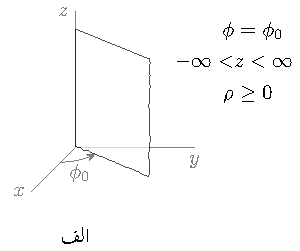
\includegraphics{figVectorCylindricalFixedAngleSurface}
\end{subfigure}%
%
\begin{subfigure}{0.5\textwidth}
\centering
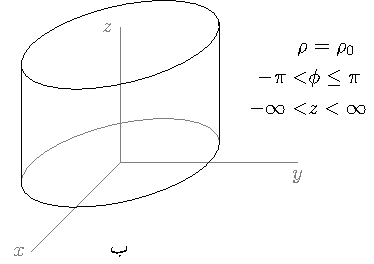
\includegraphics{figVectorCylindricalFixedRadiusSurface}
\end{subfigure}%
\caption{$\phi=\phi_0$ اور $\rho=\rho_0$ سطحیں۔}
\label{شکل_سمتیہ_نلکی_قطعی_زاویہ_سطح}
\end{figure}
\جزوحصہ{نلکی لامحدود سطحیں}
شکل \حوالہ{شکل_سمتیہ_نلکی_قطعی_زاویہ_سطح}-الف میں \عددیء{\phi} تبدیل کئے بغیر \عددیء{\rho} اور \عددیء{z} کی قیمتیں تبدیل کرتے ہوئے \عددیء{\phi=\phi_0} سطح کا حصول دکھایا گیا ہے۔یہ سطح نلکی شکل رکھتی ہے  جس کا اوپر والا منہ اور نچلا منہ کھلے ہیں یعنی ان پر ڈھکن نہیں۔شکل-ب میں \عددیء{\rho} تبدیل کئے بغیر \عددیء{\phi} اور \عددیء{z} کو تبدیل کرتے ہوئے \عددیء{\rho=\rho_0} سطح کا حصول دکھایا گیا ہے۔ان دونوں لامحدود سطحوں کے کچھ حصے ان  اشکال میں  دکھائے گئے ہیں۔ شکل-الف میں \عددیء{\rho} کی قیمت صرف مثبت جبکہ \عددیء{z} کی قیمت مثبت یا منفی ممکن ہے۔شکل-ب میں زاویہ کُل \عددیء{2\pi} ریڈیئن تبدیل ہو سکتا ہے۔یوں زاویے کا مثبت حد \عددیء{\pi} ریڈیئن یعنی \عددیء{180} درجہ ہے جبکہ اس کا منفی\حاشیہد{حقیقت میں منفی حد \عددیء{-180^\circ} کو نہیں چھوتا۔اگر منفی حد \عددیء{-180^\circ} کو چھوئے تب منفی \عددیء{x} محدد دو مرتبہ شامل ہوتا ہے۔} حد \عددیء{-\pi} یعنی \عددیء{-180} درجے ہے۔نلکی محدد اور کارتیسی نظام دونوں میں \عددیء{z=z_0}  سطح یکساں بنتی ہے۔

جیسے شکل \حوالہ{شکل_سمتیہ_نلکی_تین_سطحیں} میں دکھایا گیا ہے، \عددیء{\rho=\rho_1} اور \عددیء{\phi=\phi_1}  سطحیں \عددیء{\az} کی سیدھ میں سیدھی لکیر پر ملتے ہیں۔اسی طرح \عددیء{\rho=\rho_1} اور \عددیء{z=z_1} سطحیں ایک گول دائرے پر ملتے ہیں جبکہ \عددیء{\phi=\phi_1} اور \عددیء{z=z_1} سطحیں \عددیء{\arho} کی سیدھ میں سیدھی لکیر پر ملتے ہیں۔\عددیء{\rho=\rho_1}، \عددیء{\phi=\phi_1} اور \عددیء{z=z_1} سطحیں صرف اور صرف ایک ہی نقطہ \عددیء{N} پر اکٹھے ملتے ہیں۔نلکی محدد میں کسی بھی نقطے  کا مقام اسی طرح تین سطحوں کے  متقاطع نقطہ سے حاصل کیا جاتا ہے البتہ \عددیء{(0,0,z)} تک پہنچنے کی خاطر ایسا کرنے کی ضرورت نہیں ہوتی۔

\begin{figure}
\centering
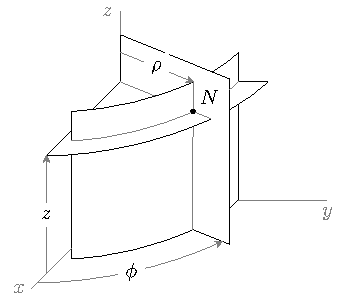
\includegraphics{figVectorCylindricalIntersectingSurfaces}
\caption{نلکی محدد کے تین سطحیں۔}
\label{شکل_سمتیہ_نلکی_تین_سطحیں}
\end{figure}
کسی بھی نقطہ \عددیء{N(\rho_1,\phi_1,z_1)} پر \عددیء{\rho=\rho_1}، \عددیء{\phi=\phi_1} اور \عددیء{z=z_1} سطحیں  بنانے کے بعد اگر نلکی محدد کے متغیرات کو \عددیء{\dif \rho}، \عددیء{\dif \phi} اور \عددیء{\dif z} بڑھا کر مزید تین سطحیں کھینچے جائیں تو یہ چھ سطحیں مل کر منحرف مکعب کو گھیریں گے جسے شکل \حوالہ{شکل_سمتیہ_نلکی_چھوٹی_حجم}-الف میں دکھایا گیا ہے۔رداسی سمت میں اس منحرف مکعب کے اطراف کی لمبائی \عددیء{\dif \rho} جبکہ \عددیء{\az}  سمت کے اطراف کی لمبائی \عددیء{\dif z} ہے۔ \عددیء{\aphi} سمت میں \عددیء{z} محدد کے قریبی  گول طرف کی لمبائی \عددیء{\rho \dif \phi} جبکہ محدد سے دور طرف کی گول لمبائی \عددیء{(\rho+\dif \rho)\dif \phi} ہے۔جیسے جیسے اس منحرف مکعب کو چھوٹا کیا جائے ویسے ویسے یہ ایک درست مکعب کی صورت اختیار کرتا ہے لہٰذا نہایت چھوٹے حجم کو مکعب تصور کرتے ہوئے اس کا حجم \عددیء{\rho \dif \rho \dif \phi \dif z} لکھا جا سکتا ہے۔
\begin{figure}
\centering
\begin{subfigure}{0.5\textwidth}
\centering
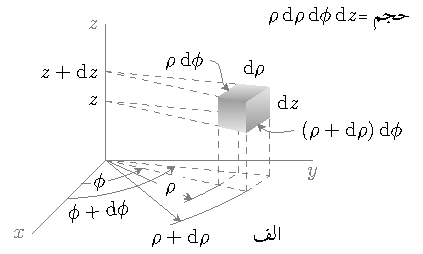
\includegraphics{figVectorCylindricalDifferentialVolume}
\end{subfigure}%
%
\begin{subfigure}{0.5\textwidth}
\centering
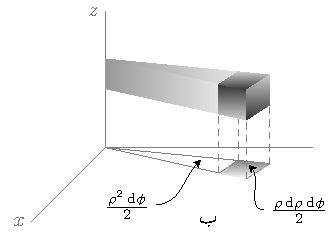
\includegraphics{figVectorCylindricalDifferentialTrapezium}
\end{subfigure}%
\caption{نلکی محدد میں انتہائی چھوٹی حجم۔}
\label{شکل_سمتیہ_نلکی_چھوٹی_حجم}
\end{figure}  

شکل \حوالہ{شکل_سمتیہ_نلکی_چھوٹی_حجم}-ب میں چھوٹے منحرف مکعب کو رداسی سمت میں \عددیء{z} محدد تک بڑھا کر پچر یا فانہ کی شکل میں دکھایا گیا ہے۔\عددیء{z=0} سطح پر اس کا عمودی سایہ بھی دکھایا گیا ہے۔\عددیء{\rho} رداس کے گول دائرے  کے مرکز سے  \عددیء{\dif \phi} زاویے پر دو لکیریں دائرے تک کھینچنے سے  \عددیء{\tfrac{\rho^2 \dif \phi}{2}} رقبہ گھیرا جاتا ہے۔اگر رداس \عددیء{\rho+\dif \rho} ہو تب رقبہ \عددیء{\tfrac{(\rho+\dif \rho)^2 \dif \phi}{2}} ہو گا۔یوں شکل-ب میں چھوٹے مکعب کے سایہ  کا رقبہ \عددیء{\dif S}
\begin{align*}
\dif S&=\frac{(\rho+\dif \rho)^2 \dif \phi}{2} - \frac{\rho^2 \dif \phi}{2}\\
&=\frac{\rho^2 \dif \phi +2 \rho \dif \rho \dif \phi+(\dif \rho)^2 \dif \phi}{2}-\frac{\rho^2 \dif \phi}{2}\\
&=\rho \dif \rho \dif \phi+\frac{(\dif \rho)^2 \dif \phi}{2}\\
&\approx \rho \dif \rho \dif \phi
\end{align*}
ہو گا۔یہاں آخری قدم پر \عددیء{\dif} کی علامت، مجموعہ کے پہلے رکن میں دو مرتبہ  جبکہ دوسرے رکن میں تین مرتبہ ہے۔یوں دوسرے اور پہلے رکن کی نسبت
  \عددیء{\tfrac{0.5(\dif \rho)^2 \dif \phi}{\rho \dif \rho \dif \phi}=\tfrac{\dif \rho}{2\rho}} ہو گی۔\عددیء{\dif \rho} کو کم سے کم\حاشیہد{کسی بھی متغیرہ مثلاً \عددیء{\rho} میں چھوٹی سی تبدیلی کو \عددیء{\Delta \rho} لکھا جاتا ہے جبکہ اس میں کم سے کم تبدیلی کو \عددیء{\dif \rho} لکھا 
جاتا ہے۔\عددیء{\dif \rho} کو تقریباً صفر سمجھا جا سکتا ہے یعنی \عددیء{\dif \rho \to 0} ہوتا ہے۔} کرتے ہوئے دوسرے رکن کو قابل نظر انداز بناتے ہوئے نظرانداز کیا گیا ہے۔یوں \عددیء{\rho \dif \rho \dif \phi} رقبہ اور \عددیء{\dif z} بلندی کے مکعب کا حجم \عددیء{\rho \dif \rho \dif \phi \dif z} ہو گا۔

شکل \حوالہ{شکل_سمتیہ_نلکی_چھوٹی_حجم} کو درست مکعب تصور کرتے ہوئے، اس کے اطراف کی لمبائی \عددیء{\rho \dif \phi}، \عددیء{\dif \rho} اور \عددیء{\dif z} لی جاتی ہے۔یوں مکعب کے نچلی اور اوپر سطح کا رقبہ مستطیل کے اطراف کو ضرب دیتے ہوئے  \عددیء{\rho \dif \rho \dif \phi} لکھا جا سکتا ہے۔اسی طرح سامنے اور پیچھے سطحوں  کا رقبہ \عددیء{\dif \rho \dif z} جبکہ بائیں اور دائیں سطحوں کا رقبہ \عددیء{\rho \dif \phi \dif z} لکھا جا سکتا ہے۔

\حصہ{کروی محدد}
سیدھی لکیروں اور سیدھی سطحوں کو کارتیسی محدد میں زیادہ آسانی سے ظاہر کیا جا سکتا ہے جبکہ نلکی سطحوں کو ظاہر کرنے کے لئے نلکی محدد بہتر ثابت ہوتا ہے۔اسی طرح کرہ اشکال کے سطحوں کو کروی محدد میں باآسانی لکھا جا سکتا ہے۔آئیں کروی نظام پر غور کریں۔

شکل \حوالہ{شکل_سمتیہ_کروی_محدد_متغیرات}-الف میں کروی محدد کے متغیرات \عددیء{r}، \عددیء{\theta} اور \عددیء{\phi} دکھائے گئے ہیں۔محدد کے مرکز سے نقطہ \عددیء{N} تک کے فاصلے \عددیء{r} کو کروی رداس پکارا جاتا ہے جبکہ \عددیء{z} محدد سے کروی رداس تک زاویے کو \عددیء{\theta} لکھا جاتا ہے۔\عددیء{x} محدد سے رداس کے عمودی سائے تک زاویہ \عددیء{\phi} ہے۔کروی اور نلکی نظام میں \عددیء{\phi} یکساں بیان کیا جاتا ہے۔رداس کی  قیمت مثبت لی جاتی ہے۔یوں \عددیء{r \ge 0} ممکن ہے۔\عددیء{\theta} کی کم سے کم قیمت \عددیء{0^\circ} اور  زیادہ سے زیادہ  قیمت \عددیء{180^\circ} ہے جبکہ \عددیء{\phi} کی کم سے کم قیمت \عددیء{0^\circ} اور زیادہ سے زیادہ قیمت \عددیء{360^\circ} ہے۔

\begin{figure}
\centering
\begin{subfigure}{0.5\textwidth}
\centering
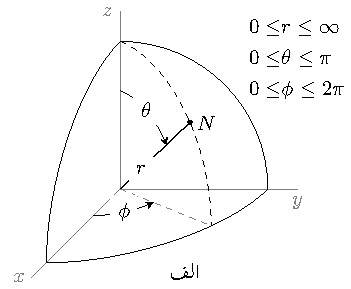
\includegraphics{figVectorSphericalRadiusThetaPhi}
\end{subfigure}%
%
\begin{subfigure}{0.5\textwidth}
\centering
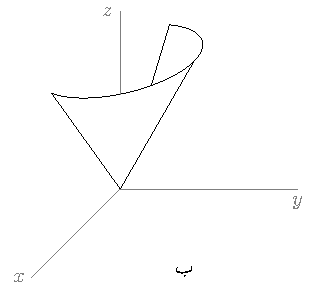
\includegraphics{figVectorSphericalThetaSurface}
\end{subfigure}%
\caption{{الف} کروی محدد کے متغیرات۔ {ب} \عددیء{\theta=\theta_0} سطح  کا کچھ حصہ۔}
\label{شکل_سمتیہ_کروی_محدد_متغیرات}
\end{figure}
%
\عددیء{r} اور \عددیء{\phi} تبدیل کئے بغیر \عددیء{\theta} کو \عددیء{0} سے بڑھاتے ہوئے \عددیء{\pi} ریڈیئن  کرنے سے نقطہ \عددیء{N}  شکل \حوالہ{شکل_سمتیہ_کروی_محدد_متغیرات}-الف میں نقطہ دار لکیر پر چلتے ہوئے  مثبت \عددیء{z} محدد سے شروع ہو کر  منفی \عددیء{z} محدد پر پہنچتا ہے۔اسے  نقطہ دار لکیر کو  کرہ ارض کے \اصطلاح{خط طول بلد}\فرہنگ{خط!طول بلد}\حاشیہب{longitude}\فرہنگ{longitude} تصور  کیا جا سکتا ہے۔  شکل-الف میں \عددیء{\theta} کا \عددیء{0^\circ} تا \عددیء{90^\circ} تبدیل ہوتا دکھایا گیا ہے۔اسی طرح \عددیء{r} اور \عددیء{\theta} تبدیل کئے بغیر \عددیء{\phi} کو \عددیء{0^\circ} تا \عددیء{360^\circ} تبدیل کرنے سے  نقطہ \عددیء{N} گول دائرے پر \عددیء{z} محدد کے گرد ایک چکر کاٹے گا۔یہ حرکت کرہ ارض کے \اصطلاح{خط عرض بلد}\فرہنگ{خط!عرض بلد}\حاشیہب{latitude}\فرہنگ{latitude} پر چلنے کے  مانند ہے۔\عددیء{\theta} اور \عددیء{\phi} تبدیل کئے بغیر \عددیء{r} کو تبدیل کرنے سے نقطہ \عددیء{N} مرکز سے  سیدھی باہر نکلتی لکیر پر حرکت کرتا ہے۔ 

\begin{figure}
\centering
\begin{subfigure}{0.5\textwidth}
\centering
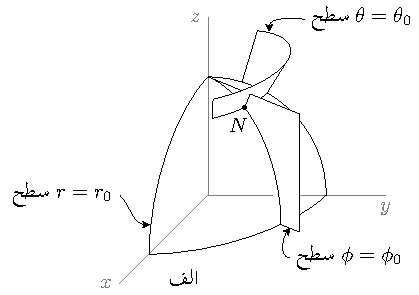
\includegraphics{figVectorSphericalIntersectingSurface}
\end{subfigure}%
%
\begin{subfigure}{0.5\textwidth}
\centering
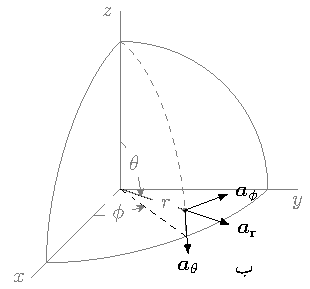
\includegraphics{figVectorSphericalUnitVectors}
\end{subfigure}%
\caption{(الف) تین عمودی سطحوں کے ملاپ سے نقطہ \عددیء{N} کا حصول۔ (ب) کروی محدد کے تین عمودی اکائی سمتیات۔}
\label{شکل_سمتیہ_کروی_تین_سطحوں_کا_مالپ}
\end{figure}

\عددیء{r} تبدیل کئے بغیر \عددیء{\theta} کو \عددیء{0^\circ} تا \عددیء{180^\circ} اور \عددیء{\phi} کو \عددیء{0^\circ} تا \عددیء{360^\circ} تبدیل کرنے سے  نقطہ \عددیء{N} کروی \عددیء{r=r_0} سطح  پر حرکت کرے گا۔ اس کروی سطح کا رداس \عددیء{r} ہو گا۔شکل \حوالہ{شکل_سمتیہ_کروی_محدد_متغیرات}-الف  میں \عددیء{\theta} کو \عددیء{0^\circ} تا \عددیء{90^\circ} اور \عددیء{\phi} کو \عددیء{0^\circ} تا \عددیء{90^\circ} تبدیل کرنے سے حاصل سطح  دکھائی گئی ہے۔شکل \حوالہ{شکل_سمتیہ_کروی_محدد_متغیرات}-ب میں \عددیء{\theta} تبدیل کئے بغیر \عددیء{r} اور \عددیء{\phi} تبدیل کرنے سے پیدا مخروط\فرہنگ{مخروط}\حاشیہب{cone}\فرہنگ{cone}  \عددیء{\theta=\theta_0}  کروی سطح دکھائی گئی ہے۔\عددیء{\phi} تبدیل کئے بغیر \عددیء{r} اور \عددیء{\theta} تبدیل کرنے سے  نلکی محدد کی طرح \عددیء{\phi=\phi_0} سطح حاصل ہوتی ہے۔ شکل \حوالہ{شکل_سمتیہ_کروی_تین_سطحوں_کا_مالپ}-الف میں ان تینوں سطحوں کو دکھایا گیا ہے۔بالکل کارتیسی اور نلکی محدد کی طرح، کسی بھی نقطہ \عددیء{N(r_0,\theta_0,\phi_0)} کا مقام ان تین سطحوں کے نقطہ ملاپ سے اخذ کیا جاتا ہے۔کسی بھی نقطہ \عددیء{N(r_0,\theta_0,\phi_0)} پر \عددیء{r=r_0}، \عددیء{\theta=\theta_0} اور \عددیء{\phi=\phi_0} سطحیں آپس میں عمودی ہوتی ہے اور یہ صرف اور صرف اسی نقطے پر اکھٹے ملتی ہیں۔

شکل \حوالہ{شکل_سمتیہ_کروی_تین_سطحوں_کا_مالپ}-ب میں کروی نظام کے تین عمودی اکائی سمتیات \عددیء{\ar}، \عددیء{\atheta} اور \عددیء{\aphi} دکھائے گئے ہیں۔نلکی محدد کی طرح کروی محدد کے عمودی اکائی سمتیات بھی مقام تبدیل کرنے سے تبدیل ہوتے ہیں۔کسی بھی نقطہ \عددیء{N(r_0,\theta_0,\phi_0)} پر \عددیء{\theta} اور \عددیء{\phi} تبدیل کئے بغیر \عددیء{r} کے بڑھتے جانب اکائی سمتیہ \عددیء{\ar} ہو گی۔اسی طرح \عددیء{\theta} بڑھانے سے نقطہ \عددیء{N} اکائی سمتیہ \عددیء{\atheta} کی جانب حرکت کرے گا جبکہ \عددیء{\phi} بڑھانے سے نقطہ \عددیء{\aphi} کی جانب حرکت کرے گا۔کارتیسی اور نلکی محدد کی طرح کروی محدد کے اکائی سمتیات کو بھی محددی نظام کے متغیرات کو کم سے کم بڑھاتے ہوئے  نقطے کی حرکت کی جانب اکائی سمتیہ کھینچنے سے حاصل کیا جاتا ہے۔

شکل \حوالہ{شکل_سمتیہ_کروی_تین_سطحوں_کا_مالپ}-الف سے واضح ہے کہ \عددیء{\ar} سمتیہ \عددیء{r=r_0} سطح کے عمودی جبکہ \عددیء{\theta=\theta_0} اور \عددیء{\phi=\phi_0} سطحوں کے متوازی ہے۔اسی طرح \عددیء{\atheta} سمتیہ \عددیء{\theta=\theta_0} سطح کے عمودی اور \عددیء{\phi=\phi_0} سطح کے متوازی پایا جاتا ہے جبکہ \عددیء{r=r_0} سطح کے ساتھ مماس بناتا ہے۔\عددیء{\aphi} سمتیہ \عددیء{\phi=\phi_0} سطح کے عمودی جبکہ \عددیء{r=r_0} اور \عددیء{\theta=\theta_0} سطحوں کے ساتھ مماس بناتا ہے۔

 
\عددیء{\ar}، \عددیء{\atheta} اور \عددیء{\aphi} کروی نظام  کے اکائی سمتیات ہیں۔\عددیء{\ar \times \atheta=\aphi} لکھنے سے  دائیں ہاتھ کا کروی نظام حاصل ہوتا ہے۔دائیں ہاتھ کے قانون میں دائیں ہاتھ کا انگوٹھا  \عددیء{r} جبکہ پہلی انگلی \عددیء{\theta}  اور دوسری انگلی \عددیء{\phi} بڑھانے سے پیدا حرکت کی سمتوں کو ظاہر کرتے ہیں۔نلکی محدد میں یہ انگلیاں \عددیء{\rho}، \عددیء{\phi} اور \عددیء{z} جبکہ کارتیسی محدد میں \عددیء{x}، \عددیء{y} اور \عددیء{z} بڑھانے سے پیدا حرکت کی سمتوں کو ظاہر کرتی ہیں۔

دائیں ہاتھ کے قانون  یا شکل \حوالہ{شکل_سمتیہ_کروی_صلیبی_ضرب_اکائی_سمتیات} کی مدد سے یوں اکائی سمتیات کے صلیبی ضرب
\begin{figure}
\centering
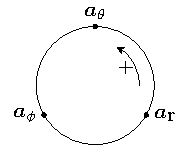
\includegraphics{figVectorSphericalRightHandCircle}
\caption{کروی نظام میں اکائی سمتیات کی صلیبی ضرب۔}
\label{شکل_سمتیہ_کروی_صلیبی_ضرب_اکائی_سمتیات}
\end{figure}

\begin{align}
\ar \times \atheta=\aphi, \quad \atheta \times \aphi=\ar, \quad \aphi \times \ar =\atheta
\end{align}

لکھے جا سکتے ہیں۔اسی طرح
\begin{align}
\ar \cdot \ar=1, \quad \atheta \cdot \atheta=1, \quad \aphi \cdot \aphi=1
\end{align}
اور
\begin{align}
\ar \cdot \atheta=0, \quad \atheta \cdot \aphi=0, \quad \aphi \cdot \ar=0
\end{align}
بھی لکھے جا سکتے ہیں۔

\begin{figure}
\centering
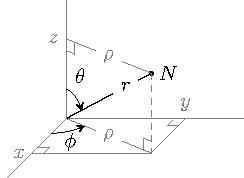
\includegraphics{figVectorSphericalToCylindricalAndCartesian}
\caption{کروی، نلکی اور کارتیسی متغیرات کا تبادلہ۔}
\label{شکل_سمتیہ_کروی_نلکی_متغیرات_تبادلہ}
\end{figure}

نقطہ \عددیء{N} کا \عددیء{z} محدد سے فاصلہ  \عددیء{\rho} ہے جو نلکی محدد کا رداس ہے۔اسے شکل \حوالہ{شکل_سمتیہ_کروی_نلکی_متغیرات_تبادلہ} میں دکھایا گیا ہے جہاں سے واضح ہے کہ \عددیء{\rho=r \sin \theta} کے برابر ہے۔اسی طرح \عددیء{z=0} سطح سے \عددیء{N} کی اونچائی \عددیء{z} ہے جو شکل کو دیکھتے ہوئے \عددیء{z=r\cos \theta}  لکھی جا سکتی ہے۔نقطہ \عددیء{N} کا عمودی سایہ \عددیء{z=0} سطح پر دکھایا گیا ہے جہاں سے واضح ہے کہ \عددیء{x=\rho \cos \phi} اور \عددیء{y=\rho \sin \phi} لکھے جا سکتے ہیں۔\عددیء{\rho=r \sin \theta} پُر کرنے سے
\begin{gather}
\begin{aligned}\label{مساوات_سمتیہ_کروی_سے_کارتیسی}
x&=r \sin \theta \cos \phi\\
y&=r \sin \theta \sin \phi\\
z&=r \cos \theta
\end{aligned}
\end{gather}
لکھے جا سکتے ہیں جہاں \عددیء{z} کی مساوات بھی ساتھ ہی لکھی  گئی ہے۔مساوات \حوالہ{مساوات_سمتیہ_کروی_سے_کارتیسی} کروی سے کارتیسی متغیرات دیتا ہے۔ اسی شکل کو دیکھتے ہوئے مسئلہ فیثاغورث کی مدد سے 
\begin{gather}
\begin{aligned}
r^2&=\rho^2+z^2\\
\rho^2&=x^2+y^2
\end{aligned}
\end{gather}
لکھتے ہوئے
\begin{align}\label{مساوات_سمتیہ_کروی_رداس}
r^2=x^2+y^2+z^2
\end{align}
حاصل ہوتا ہے۔مساوات \حوالہ{مساوات_سمتیہ_کروی_سے_کارتیسی} میں \عددیء{z} کی مساوات سے
\begin{align}\label{مساوات_سمتیہ_کروی_تھیٹا}
\theta = \cos^{-1} \frac{z}{r}=\cos^{-1}\frac{z}{\sqrt{x^2+y^2+z^2}}
\end{align}
 لکھا جا سکتا ہے۔اسی طرح  مساوات \حوالہ{مساوات_سمتیہ_کروی_سے_کارتیسی} کے \عددیء{y} کو \عددیء{x} سے تقسیم کرتے ہوئے
\begin{align}\label{مساوات_سمتیہ_کروی_فائے}
\phi = \tan^{-1} \frac{y}{x}
\end{align}
حاصل ہوتا ہے۔مساوات \حوالہ{مساوات_سمتیہ_کروی_رداس}، مساوات \حوالہ{مساوات_سمتیہ_کروی_تھیٹا} اور مساوات \حوالہ{مساوات_سمتیہ_کروی_فائے} کارتیسی سے کروی متغیرات دیتے ہیں۔
\begin{figure}
\centering
\begin{subfigure}{0.5\textwidth}
\centering
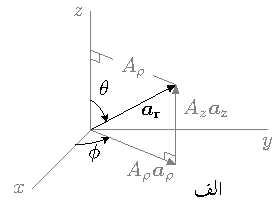
\includegraphics{figVectorSphericalUnitRadial}
\end{subfigure}%
%
\begin{subfigure}{0.5\textwidth}
\centering
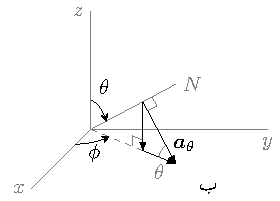
\includegraphics{figVectorSphericalUnitTheta}
\end{subfigure}%
\caption{کروی اکائی سمتیات کا کارتیسی نظام میں تبادلہ۔}
\label{شکل_سمتیہ_کروی_اکائی_رداسی_سمتیہ_کارتیسی}
\end{figure}

شکل \حوالہ{شکل_سمتیہ_کروی_تین_سطحوں_کا_مالپ}-ب میں نقطہ \عددیء{N} پر اکائی سمتیات دکھائے گئے ہیں۔\عددیء{\ar} کی سمت تبدیل کئے بغیر اسے محدد کے مرکز پر منتقل کرتے ہوئے شکل \حوالہ{شکل_سمتیہ_کروی_اکائی_رداسی_سمتیہ_کارتیسی}-الف  میں دکھایا گیا ہے جہاں سے ظاہر ہے کہ اسے نلکی محدد کے اکائی سمتیات کی مدد سے
\begin{align}
\ar=A_\rho \arho+A_z \az
\end{align}
لکھا جا سکتا ہے۔شکل \حوالہ{شکل_سمتیہ_کروی_اکائی_رداسی_سمتیہ_کارتیسی}-الف  میں \عددیء{\ar} کی لمبائی ایک لیتے ہوئے  \عددیء{A_\rho=\sin \theta} اور \عددیء{A_z=\cos \theta} لکھا جا سکتا ہے۔یوں
\begin{align}\label{مساوات_سمتیہ_کروی_اکائی_نلکی_منتقل}
\ar=\sin \theta \arho+\cos \theta \az
\end{align}
حاصل ہوتا ہے۔اس مساوات کا باری باری \عددیء{\arho}، \عددیء{\aphi} اور \عددیء{\az} کے ساتھ غیر سمتی ضرب لیتے ہوئے
\begin{gather}
\begin{aligned}\label{مساوات_سمتیہ_کروی_رداس_نلکی_اکائی_غیر_سمتی_ضرب}
\ar \cdot \arho&=(\sin \theta \arho+\cos \theta \az) \cdot \arho=\sin \theta\\
\ar \cdot \aphi&=(\sin \theta \arho+\cos \theta \az) \cdot \aphi=0\\
\ar \cdot \az&=(\sin \theta \arho+\cos \theta \az) \cdot \az=\cos \theta
\end{aligned}
\end{gather}
حاصل ہوتا ہے جہاں \عددیء{\arho \cdot \arho=1}، \عددیء{\az \cdot \arho=0} وغیرہ کا استعمال کیا گیا۔یہ مساوات کروی رداسی اکائی سمتیے اور نلکی نظام کے اکائی سمتیات کے تمام ممکنہ غیر سمتی ضرب دیتا ہے۔اسی طرح جدول \حوالہ{جدول_سمتیہ_نلکی_کارتیسی_اکائی_غیر-سمتی_ضرب} استعمال کرتے ہوئے  مساوات  \حوالہ{مساوات_سمتیہ_کروی_اکائی_نلکی_منتقل} کا باری باری \عددیء{\ax} اور \عددیء{\ay} کے ساتھ غیر سمتی ضرب لیتے ہوئے
\begin{gather}
\begin{aligned}\label{مساوات_سمتیہ_کروی_رداس_کے_کارتیسی_اجزاء}
\ar \cdot \ax&=(\sin \theta \arho+\cos \theta \az) \cdot \ax=\sin \theta \cos \phi\\
\ar \cdot \ay&=(\sin \theta \arho+\cos \theta \az) \cdot \ay=\sin \theta \sin \phi\\
\ar \cdot \az&=(\sin \theta \arho+\cos \theta \az) \cdot \az=\cos \theta
\end{aligned}
\end{gather}
حاصل ہوتا ہے۔مکمل نتائج ایک جگہ لکھنے کی خاطر  مندرجہ بالا مساوات میں  \عددیء{\ar \cdot \az} کو بھی شامل کیا گیا ہے۔ یہ مساوات کروی اکائی رداسی  سمتیے  اور کارتیسی اکائی سمتیات کے تمام ممکنہ غیر سمتی ضرب دیتا ہے۔

\عددیء{\ar} کو کارتیسی نظام میں لکھنے کی خاطر \عددیء{\ar=\kvec{A}=A_x \ax+A_y \ay+A_z \az} لکھتے ہیں۔مساوات \حوالہ{مساوات_سمتیہ_کارتیسی_اجزاء} کے مطابق \عددیء{A_x=\ax \cdot \ar} جبکہ \عددیء{A_y=\ay \cdot \ar} اور \عددیء{A_z=\az \cdot \ar} ہوں گے۔یہ تمام  مساوات \حوالہ{مساوات_سمتیہ_کروی_رداس_کے_کارتیسی_اجزاء} میں دئے گئے ہیں۔ یوں 
\begin{align}
\ar=\sin \theta \cos \phi \ax+\sin \theta \sin \phi \ay+\cos \theta \az
\end{align}
لکھا جا سکتا ہے۔

شکل \حوالہ{شکل_سمتیہ_کروی_تین_سطحوں_کا_مالپ}-ب میں دکھائے \عددیء{\atheta} کو \عددیء{\phi=\phi_0} سطح پر حرکت دیتے ہوئے  مرکز کے اتنے قریب لا کر شکل \حوالہ{شکل_سمتیہ_کروی_اکائی_رداسی_سمتیہ_کارتیسی}-ب میں دکھایا گیا ہے کہ اس کی نوک \عددیء{x=0} سطح کو چھوتی ہے۔جیسا شکل \حوالہ{شکل_سمتیہ_کروی_تین_سطحوں_کا_مالپ}-الف سے واضح ہے،  \عددیء{\phi=\phi_0} سطح پر \عددیء{\atheta} کو حرکت دینے سے اس سمتیہ کی سمت تبدیل نہیں ہوتی۔شکل \حوالہ{شکل_سمتیہ_کروی_اکائی_رداسی_سمتیہ_کارتیسی}-ب کو دیکھتے ہوئے \عددیء{\atheta=B_\rho \arho-B_z \az} لکھا جا سکتا ہے۔یہاں رک کر  تسلی کر لیں کہ \عددیء{B_\rho \arho} اور \عددیء{\atheta} کے مابین زاویہ \عددیء{\theta} ہے۔\عددیء{\atheta}، \عددیء{B_\rho \arho} اور \عددیء{-B_z \az} مل کر تکون بناتے ہیں جسے دیکھتے ہوئے مسئلہ فیثاغورث کی مدد سے
\begin{align*}
B_\rho&=\cos \theta\\
B_z&=\sin \theta
\end{align*}
لکھا جا سکتا ہے۔یوں
\begin{align}\label{مساوات_سمتیہ_کروی_اکائی_تھیٹا}
\atheta=\cos \theta \arho-\sin \theta \az
\end{align}
کے برابر ہے۔اس مساوات کا باری باری \عددیء{\arho}، \عددیء{\aphi} اور \عددیء{\az} کے ساتھ غیر سمتی ضرب لینے سے
\begin{gather}
\begin{aligned}\label{مساوات_سمتیہ_کروی_تھیٹا_نلکی_اکائی_غیر_سمتی_ضرب}
\atheta \cdot \arho&=(\cos \theta \arho-\sin \theta \az) \cdot \arho=\cos \theta\\
\atheta \cdot \aphi&=(\cos \theta \arho-\sin \theta \az) \cdot \aphi=0\\
\atheta \cdot \az&=(\cos \theta \arho-\sin \theta \az) \cdot \az=-\sin \theta
\end{aligned}
\end{gather}
\عددیء{\atheta} اور نلکی اکائی سمتیات کے  تمام غیر سمتی ضرب حاصل ہوتے ہیں۔اسی طرح مساوات \حوالہ{مساوات_سمتیہ_کروی_اکائی_تھیٹا} کا باری باری \عددیء{ax}، \عددیء{\ay} اور \عددیء{\az} کے ساتھ غیر سمتی ضرب لینے سے
\begin{gather}
\begin{aligned}\label{مساوات_سمتیہ_کروی_تھیٹا_کے_کارتیسی_اجزاء}
\atheta \cdot \ax&=(\cos \theta \arho-\sin \theta \az) \cdot \ax=\cos \theta \arho \cdot \ax=\cos \theta \cos \phi\\
\atheta \cdot \ay&=(\cos \theta \arho-\sin \theta \az) \cdot \ay=\cos \theta \arho \cdot \ay=\cos \theta \sin \phi \\
\atheta \cdot \az&=(\cos \theta \arho-\sin \theta \az) \cdot \az=-\sin \theta \az \cdot \az=-\sin \theta
\end{aligned}
\end{gather}
حاصل ہوتے ہیں۔یہ مساوات \عددیء{\atheta} اور کارتیسی اکائی سمتیات کے تمام غیر سمتی ضرب دیتا ہے۔

\عددیء{\atheta} کو کارتیسی نظام میں لکھنے کی خاطر \عددیء{\atheta=\kvec{A}=A_x \ax+A_y\ay+A_z\az} لکھتے ہیں۔مساوات \حوالہ{مساوات_سمتیہ_کارتیسی_اجزاء} کے مطابق \عددیء{A_x=\ax \cdot \atheta} جبکہ \عددیء{A_y=\ay \cdot \atheta} اور \عددیء{A_z=\az \cdot \atheta} ہوں گے۔یہ تمام  مساوات \حوالہ{مساوات_سمتیہ_کروی_تھیٹا_کے_کارتیسی_اجزاء} میں دئے گئے ہیں۔ یوں
\begin{align}
\atheta=\cos \theta \cos \phi \ax+\cos \theta \sin \phi\ay-\sin \theta\az
\end{align}  
لکھا جا سکتا ہے۔

کروی  محدد کا \عددیء{\aphi} اور نلکی محدد کا \عددیء{\aphi} یکساں ہیں۔اسے کارتیسی نظام میں
\begin{align}
\aphi=-\sin \phi \ax+\cos \phi \ay
\end{align} 
لکھا جاتا ہے۔اس مساوات کا \عددیء{\ax}، \عددیء{\ay} اور \عددیء{\az} کے ساتھ غیر سمتی ضرب لیتے ہوئے
\begin{gather}
\begin{aligned}
\aphi \cdot \ax&=-\sin \phi\\
\aphi \cdot \ay&=\cos \phi\\
\aphi \cdot \az&=0
\end{aligned}
\end{gather}
لکھا جا سکتا ہے۔

مساوات \حوالہ{مساوات_سمتیہ_کروی_رداس_نلکی_اکائی_غیر_سمتی_ضرب} اور مساوات \حوالہ{مساوات_سمتیہ_کروی_تھیٹا_نلکی_اکائی_غیر_سمتی_ضرب} کے نتائج کے ساتھ \عددیء{\aphi} کے مختلف غیر سمتی ضربوں کو جدول \حوالہ{جدول_سمتیہ_کروی_نلکی_اکائی_غیر-سمتی_ضرب} میں یکجا کیا گیا ہے۔

\begin{table}
\caption{کروی  اکائی سمتیات کا نلکی اکائی سمتیات کے ساتھ غیر سمتی ضرب۔}
\centering
\begin{tabular}{l | r r r}
 & $\arho$ & $\aphi$ & $\az$ \\
\hline
$\ar$ & $\sin \theta$ & $0$& $\cos \theta$\\
$\atheta$ &$\cos \theta$ &$ 0$ &$ -\sin \theta$\\
$\aphi$ & $0$ &$ 1$ &$0$
\end{tabular}
\label{جدول_سمتیہ_کروی_نلکی_اکائی_غیر-سمتی_ضرب}
\end{table}
%

مساوات  \حوالہ{مساوات_سمتیہ_کروی_رداس_کے_کارتیسی_اجزاء} اور مساوات  \حوالہ{مساوات_سمتیہ_کروی_تھیٹا_کے_کارتیسی_اجزاء} کے نتائج جدول \حوالہ{جدول_سمتیہ_کروی_کارتیسی_اکائی_غیر-سمتی_ضرب} میں یکجا کئے گئے ہیں۔ 
\begin{table}
\caption{کروی  اکائی سمتیات کا کارتیسی اکائی سمتیات کے ساتھ غیر سمتی ضرب۔}
\centering
\begin{tabular}{l | r r r}
 & $\ax$ & $\ay$ & $\az$ \\
\hline
$\ar$ & $\sin \theta \cos \phi$ & $\sin \theta \sin \phi$& $\cos \theta$\\
$\atheta$ &$\cos \theta \cos \phi$ &$ \cos \theta \sin \phi$ &$ -\sin \theta$\\
$\aphi$ & $-\sin \phi$ &$ \cos \phi$ &$0$
\end{tabular}
\label{جدول_سمتیہ_کروی_کارتیسی_اکائی_غیر-سمتی_ضرب}
\end{table}
%
\begin{figure}
\centering
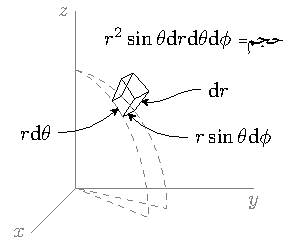
\includegraphics{figVectorSphericalDifferentialVolume}
\caption{کروی نظام میں چھوٹی حجم۔}
\label{شکل_سمتیہ_کروی_چھوٹی_حجم}
\end{figure}

شکل \حوالہ{شکل_سمتیہ_کروی_تین_سطحوں_کا_مالپ} میں \عددیء{N(r,\theta,\phi)} پر تین عمودی سطحیں دکھائی گئی ہیں۔اگر کروی محدد کے متغیرات \عددیء{\dif r}، \عددیء{\dif \theta} اور \عددیء{\dif \phi} بڑھا کر دوبارہ تین عمودی سطحیں کھینچی جائیں تو یہ چھ سطحیں مل کر چھوٹا منحرف مکعب نما حجم گھیریں گی جسے شکل \حوالہ{شکل_سمتیہ_کروی_چھوٹی_حجم} میں دکھایا گیا ہے۔\عددیء{\ar} سمت میں مکعب کے چار اطراف کی لمبائیاں \عددیء{\dif r} ہے۔\عددیء{\atheta} سمت میں \عددیء{z} محدد کے قریبی دو اطراف کی لمبائیاں \عددیء{r \dif \theta} جبکہ دو دور اطراف کی لمبائیاں \عددیء{(r+\dif r)\dif \theta} ہے جسے دو اجزاء کی صورت میں یوں  \عددیء{r \dif \theta +\dif r \dif \theta} لکھا جا سکتا ہے۔دور اطراف کے لمبائی کا پہلا جزو ہوبہو قریبی اطراف کی لمبائی ہے جبکہ اس کا دوسرا جزو دور اور قریبی اطراف کے لمبائیوں میں فرق کو ظاہر کرتی ہے۔ان دو اجزاء کی نسبت \عددیء{\tfrac{\dif r \dif \theta}{r \dif \theta}=\tfrac{\dif r}{r}}  کے برابر ہے۔\عددیء{\dif r} کو کم سے کم\حاشیہد{کسی بھی متغیرہ مثلاً \عددیء{r} میں چھوٹی سی تبدیلی کو \عددیء{\Delta r} لکھا جاتا ہے جبکہ اس میں کم سے کم تبدیلی کو \عددیء{\dif r} لکھا جاتا ہے۔\عددیء{\dif r} کو تقریباً صفر سمجھا جا سکتا ہے یعنی \عددیء{\dif r \to 0} ہوتا ہے۔} کرتے ہوئے اس نسبت کو کم سے کم کیا جا سکتا  ہے۔ایسا ہی کرتے ہوئے ہم \عددیء{\dif r \dif \theta} کو رد کرتے ہوئے ان چاروں اطراف کی لمبائیاں \عددیء{r \dif \theta} ہی لیتے ہیں۔اسی طریقہ کار سے  \عددیء{\aphi} اطراف کی لمبائیاں  \عددیء{r \sin \theta \dif \phi} لکھی جا سکتی ہے۔منحرف مکعب نما کے اطراف میں معمولی فرق کو نظرانداز کرتے ہوئے اسے مکعب نما تصور کیا جا سکتا ہے جس کے \عددیء{r=r_0} سطحوں کا رقبہ \عددیء{r^2 \sin \theta \dif \theta \dif \phi} جبکہ \عددیء{\theta=\theta_0} سطحوں کا رقبہ \عددیء{r \sin \theta \dif r \dif \phi} اور \عددیء{\phi=\phi_0} سطحوں کا رقبہ   \عددیء{r \dif r \dif \theta} ہو گا۔اس مکعب کا حجم \عددیء{r^2 \sin \theta \dif r \dif \theta \dif \phi} ہو گا۔

کسی بھی مکمل بند سطح کی  سمت، سطح کے عمودی باہر جانب لی جاتی ہے۔شکل \حوالہ{شکل_سمتیہ_کروی_چھوٹی_حجم} میں \عددیء{r=r_0} سطح  مرکز کا قریبی سطح ہے۔اس سطح کے دو آپس میں الٹ عمودی اطراف \عددیء{\mp \ar} ہیں جن میں \عددیء{-\ar} بند سطح کی بیرونی سمت کو ظاہر کرتا ہے لہٰذا یہی اس سطح کی درست سمت ہے۔اس کے برعکس \عددیء{r=r_0+\dif r} سطح مرکز سے دور تر ہے۔اس سطح کے بھی دو آپس میں الٹ عمودی سمتیں \عددیء{\mp \ar} ہیں جن میں \عددیء{\ar} سطح کی درست سمت ہے۔یوں  \عددیء{r=r_0} سطح کا سمتی رقبہ \عددیء{-r^2 \sin \theta \dif \theta \dif \phi \ar} جبکہ \عددیء{r=r_0+\dif r} سطح کا سمتی رقبہ \عددیء{\عددیء{r^2 \sin \theta \dif \theta \dif \phi \ar}} ہے۔اسی طرح \عددیء{\theta=\theta_0} سطح کا سمتی رقبہ \عددیء{-r \sin \theta \dif r \dif \phi\atheta} جبکہ \عددیء{\theta=\theta_0+\dif \theta} سطح کا سمتی رقبہ\عددی{r \sin \theta \dif r \dif \phi\atheta} ہو گا۔\عددیء{\phi=\phi_0} سطح کا \عددیء{-r \dif r \dif \theta \aphi} اور \عددیء{\phi=\phi_0+\dif \phi} سطح کا سمتی رقبہ \عددیء{r \dif r \dif \theta \aphi} ہو گا۔

%===================
\ابتدا{مشق}
شکل \حوالہ{شکل_سمتیہ_کروی_چھوٹی_حجم} میں \عددیء{} سمت میں مرکز کے قریبی اور دور اطراف کی لمبائیاں لکھیں۔

جوابات:\عددیء{r \sin \theta \dif \phi}، \عددیء{r \sin(\theta+\dif \theta) \dif \phi}، \عددیء{(r+\dif r) \sin \theta \dif \phi} اور \عددیء{(r+\dif r) \sin(\theta+\dif \theta) \dif \phi}
\انتہا{مشق}
%=======================
\ابتدا{مثال}\شناخت{مثال_سمتیہ_نلکی_کارتیسی_غیر_سمتی_اکائی_ضرب}
دو اکائی سمتیات \عددیء{\kvec{a}_1} اور \عددیء{\kvec{a}_2} کا غیر سمتی ضرب \عددیء{\kvec{a}_1 \cdot \kvec{a}_2=(1)(1) \cos \alpha_{12}} یعنی ان کے مابین زاویے \عددیء{\alpha_{12}} کے کوسائن کے برابر ہوتا ہے۔غیر سمتی ضرب کے اس تعریف کو استعمال کرتے ہوئے \عددیء{\ax \cdot \arho}، \عددیء{\ay \cdot \arho}، \عددیء{\ax \cdot \aphi} اور \عددیء{\ay \cdot \aphi} حاصل کریں۔
\begin{figure}
\centering
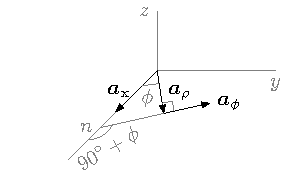
\includegraphics{figVectorDotProductUnitCartesianAndCylindrical}
\caption{کارتیسی اور نلکی اکائی سمتیات کا غیر سمتی ضرب۔}
\label{شکل_سمتیہ_غیر_سمتی_ضرب_بذریعہ_تعریف}
\end{figure}

حل:شکل \حوالہ{شکل_سمتیہ_غیر_سمتی_ضرب_بذریعہ_تعریف} میں \عددیء{\ax} اور \عددیء{\arho} کے درمیان زاویہ \عددیء{\phi} جبکہ \عددیء{\ay} اور \عددیء{\arho} کے درمیان زاویہ \عددیء{90^\circ-\phi} پایا جاتا ہے لہٰذا \عددیء{\ax \cdot \arho=\cos \phi} اور \عددیء{\ay \cdot \arho=\cos (90^\circ-\phi)=\sin \phi} کے برابر ہیں۔\عددیء{\ax} اور \عددیء{\aphi} کی سمتیں تبدیل کئے بغیر اگر انہیں یوں ہلایا جائے کہ ان کی دُم نقطہ \عددیء{n} پر آ ٹھرے تو شکل سے ظاہر ہے کہ ان کے مابین زاویہ \عددیء{90^\circ+\phi} ہے۔یوں \عددیء{\ax \cdot \aphi=\cos (90^\circ+\phi)=-\sin \phi} کے برابر ہے۔اسی طرح \عددیء{\ay} اور \عددیء{\aphi} کے درمیان \عددیء{\phi} زاویہ ہونے کی بنا پر \عددیء{\ay \cdot \aphi=\cos \phi} کے برابر ہے۔چونکہ \عددیء{\az} ان دونوں نلکی اکائی سمتیات کے عمودی ہے لہٰذا ان کا غیر سمتی ضرب صفر کے برابر ہو گا۔  
\انتہا{مثال}
%============
\begin{figure}
\centering
\begin{subfigure}{0.5\textwidth}
\centering
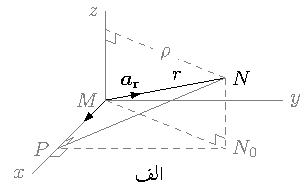
\includegraphics{figVectorSphericalUnitRadialDotWithCartesian}
\end{subfigure}%
%
\begin{subfigure}{0.5\textwidth}
\centering
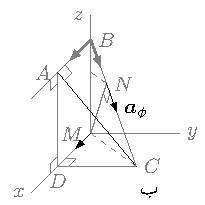
\includegraphics{figVectorSphericalUnitThetaDotWithCartesian}
\end{subfigure}%
\caption{کروی اور کارتیسی اکائی سمتیات کا غیر سمتی ضرب۔}
\label{شکل_سمتیہ_کروی_کارتیسی_اکائی_غیر_سمتی_ضرب}
\end{figure}

\ابتدا{مثال}
مثال \حوالہ{مثال_سمتیہ_نلکی_کارتیسی_غیر_سمتی_اکائی_ضرب} کے طرز پر \عددیء{\ar}  کا \عددیء{\ax}، \عددیء{\ay} اور \عددیء{\az} کے ساتھ غیر سمتی ضرب حاصل کریں۔

حل: شکل \حوالہ{شکل_سمتیہ_کروی_کارتیسی_اکائی_غیر_سمتی_ضرب}-الف میں نقطہ \عددیء{N(r,\theta,\phi)} دکھایا گیا ہے جسے \عددیء{N(x,y,z)} بھی لکھا جا سکتا ہے۔شکل میں \عددیء{\ax} اور \عددیء{\ar} بھی دکھائے گئے ہیں۔شکل سے ظاہر ہے کہ \عددیء{\ax \cdot \ar=\cos \phase{NMP}} کے برابر ہے جہاں \عددیء{N} اور \عددیء{P} سے \عددیء{M} تک لکیریں کھینچنے سے زاویہ \عددیء{\phase{NMP}} بنتا ہے۔\عددیء{N} سے \عددیء{z=0} سطح پر عمود نقطہ \عددیء{N_0} دیتا ہے۔\عددیء{N_0} سے \عددیء{x} محدد پر عمود نقطہ \عددیء{P} دیتا ہے۔\عددیء{N} سے \عددیء{N_0} اور یہاں سے \عددیء{P} منتقل ہوتے ہوئے \عددیء{\ax} سمت میں کسی قسم کی حرکت نہیں کی جاتی لہٰذا اگر کارتیسی نظام میں \عددیء{N(x,y,z)} لکھا جائے تو اسی نظام میں \عددیء{N_0(x,y,0)} اور  \عددیء{P(x,0,0)} لکھے جائیں گے۔ہم \عددیء{N} سے \عددیء{x} محدد پر عمود بناتے ہوئے بھی \عددیء{P} تک پہنچ سکتے ہیں۔ تکون \عددیء{NMP} میں \عددیء{M} سے \عددیء{N} تک کا فاصلہ \عددیء{\overline{MN}=r} جبکہ \عددیء{M} سے \عددیء{P} تک کا فاصلہ \عددیء{\overline{MP}=x} اور زاویہ \عددیء{\phase{NPM}=90^\circ} ہیں لہٰذا \عددیء{\cos \phase{NMP}=\tfrac{x}{r}} ہو گا۔یہی  \عددیء{\ax} اور \عددیء{\ar} کے غیر سمتی ضرب  کے برابر ہے۔\عددیء{N} سے \عددیء{y} محدد پر عمود بناتے ہوئے یوں \عددیء{\ay \cdot \ar=\tfrac{y}{r}} اور \عددیء{N} سے \عددیء{z} محدد پر عمود سے \عددیء{\az \cdot \ar=\tfrac{z}{r}} لکھے جا سکتے ہیں۔چونکہ \عددیء{x=r\sin \theta \cos \phi}، \عددیء{y=r\sin \theta \sin \phi} اور \عددیء{z=r\cos \theta} کے برابر  ہیں لہٰذا ہم
\begin{align*}
\ar \cdot \ax&=\frac{x}{r}=\sin \theta \cos \phi\\
\ar \cdot \ay&=\frac{y}{r}=\sin \theta \sin \phi\\
\ar \cdot \az&=\frac{z}{r}=\cos \theta
\end{align*}
لکھ سکتے ہیں۔
\انتہا{مثال}
%=======================
\ابتدا{مثال}
مثال \حوالہ{مثال_سمتیہ_نلکی_کارتیسی_غیر_سمتی_اکائی_ضرب} کے طرز پر \عددیء{\atheta}  کا \عددیء{\ax} کے ساتھ غیر سمتی ضرب حاصل کریں۔

حل: شکل \حوالہ{شکل_سمتیہ_کروی_کارتیسی_اکائی_غیر_سمتی_ضرب}-ب میں نقطہ \عددیء{N} پر اکائی سمتیہ \عددیء{\atheta} جبکہ محدد کے مرکز \عددیء{M} پر \عددیء{\ax} دکھائے گئے ہیں۔\عددیء{\atheta \cdot \ax} حاصل کرنے کی خاطر سمتیات کی سمت تبدیل کئے بغیر انہیں \عددیء{z} محدد پر نقطہ \عددیء{B} منتقل کرتے ہوئے دوبارہ دکھایا گیا ہے جہاں سے واضح ہے کہ \عددیء{\atheta \cdot \ax=\cos \phase{ABC}} کے برابر ہے۔اس شکل میں \عددیء{\phase{DMC}=\phi} اور \عددیء{\phase{BMN}=\theta} کروی محدد کے زاویے ہیں۔تکون \عددیء{\Delta BMN} میں زاویہ \عددیء{\phase{MNB}} نوے درجے کا ہے۔یوں \عددیء{\phase{NBM}=90^\circ-\theta} ہو گا۔شکل سے واضح ہے کہ  \عددیء{\phase{NBM}=\phase{CBM}} ہیں۔اس طرح تکون \عددیء{\Delta BMC} میں \عددیء{\phase{BMC}=90^\circ} جبکہ \عددیء{\phase{CBM}=90^\circ-\theta} ہونے کی بنا پر \عددیء{\phase{MCB}=\theta} ہو گا۔

شکل-ب میں \عددیء{\overline{BM}=z} لیتے ہوئے تکون \عددیء{\Delta BMC}   کو دیکھتے ہوئے
\begin{align*}
\overline{BC}&=\frac{z}{\sin \theta}   \\
\overline{MC}&=\frac{z}{\tan \theta} 
\end{align*}
لکھا جا سکتا ہے۔تکون \عددیء{\Delta MDC} سے
\begin{align*}
\overline{MD}&=\overline{MC} \cos \phi=\frac{z \cos \phi}{\tan \theta} 
\end{align*} 
لکھا جا سکتا ہے۔شکل سے واضح ہے کہ \عددیء{\overline{MD}} اور \عددیء{\overline{AB}} برابر ہیں یعنی \عددیء{\overline{AB}=\overline{MD}}-یوں تکون \عددیء{\Delta BAC} سے
\begin{align*}
\cos \phase{ABC}&=\frac{\overline{AB}}{\overline{BC}}=\frac{\left(\frac{z \cos \phi}{\tan \theta}\right)}{\left(\frac{z}{\sin \theta}\right)}=\cos \theta \cos \phi
\end{align*}
حاصل ہوتا ہے۔یوں \عددیء{\ar \cdot \ax=\cos \theta \cos \phi} لکھا جا سکتا ہے۔
\انتہا{مثال}
%============

\ابتدا{مشق}
شکل \حوالہ{شکل_سمتیہ_کروی_کارتیسی_اکائی_غیر_سمتی_ضرب}-ب کے طرز پر شکل بناتے ہوئے \عددیء{\atheta \cdot \ay} اور \عددیء{\atheta \cdot \ay} حاصل کریں۔

جوابات:\عددیء{\cos \theta \sin \phi} اور \عددیء{-\sin \theta}
\انتہا{مشق}
%============

\باب{کولومب کا قانون}
\حصہ{قوت کشش یا دفع}
نیوٹن کے \اصطلاح{کائناتی تجاذب کے قانون}\فرہنگ{تجاذب}\حاشیہب{Law of Universal Gravitation} سے آپ بخوبی واقف ہوں گے۔\اصطلاح{کولومب کا قانون}\فرہنگ{کولومب کا قانون}\حاشیہب{Coulomb's law} اس سے قریبی مشابہت رکھتا ہے۔کائناتی تجاذب کے قانون کو مساوات \حوالہ{مساوات_کولوم_کشش_ثقل} میں پیش کیا گیا ہے۔
\begin{align}\label{مساوات_کولوم_کشش_ثقل}
F&=G \frac{M_1 M_2}{R^2}
\end{align}
یہ مساوات کمیت \عددیء{M_1} اور کمیت \عددیء{M_2} کے مابین قوت کشش \عددیء{F} دیتا ہے جہاں ایک کمیت کے مرکز سے دوسری کمیت کے مرکز تک کا فاصلہ \عددیء{R} ہے۔قوت کشش دونوں کمیت کے حاصل ضرب کے  راست متناسب اور ان کے مرکزوں کے درمیانی فاصلے  کے مربع کے بالعکس متناسب ہوتی ہے۔دونوں کمیتوں پر قوت کشش کی مقدار برابر ہوتی ہے اور یہ قوت دونوں کمیتوں کے  مرکزوں پر کھینچی لکیر پر عمل درآمد ہوتی ہے۔\عددیء{M_1} پر قوت کشش کی سمت \عددیء{M_1} کے مرکز سے \عددیء{M_2} کے مرکز کی جانب کو ہوتا ہے جبکہ \عددیء{M_2} پر قوت کشش کی سمت \عددیء{M_2} کے مرکز سے \عددیء{M_1} کے مرکز کی جانب کو ہوتا ہے۔تناسب کے جزو مستقل کو \عددیء{G} لکھا اور \اصطلاح{تجاذبی مستقل}\فرہنگ{تجاذبی مستقل}\حاشیہب{gravitational constant}\فرہنگ{gravitational constant} پکارا جاتا ہے جس کی قیمت تقریباً \عددیء{\SI{6.674e-11}{\meter \cubed \per \kilo \gram \per \second \squared}} کے برابر ہے۔

کولومب کا قانون مساوات \حوالہ{مساوات_کولوم_کولومب_کشش_چارج} میں بیان کیا گیا ہے۔یہ مساوات چارج \عددیء{Q_1} اور چارج \عددیء{Q_2} کے مابین قوت کشش یا قوت دفع \عددیء{F} دیتا ہے جہاں ایک چارج کے مرکز سے دوسری چارج کے مرکز تک کا فاصلہ \عددیء{R} ہے۔ان چارجوں کا حجم صفر تصور کیا جاتا ہے۔یوں اگر چارج کو گیند کی شکل کا تصور کیا جائے تو اس گیند کے رداس  کی لمبائی صفر ہو گی۔ایسے چارج کو \اصطلاح{نقطہ چارج}\فرہنگ{نقطہ چارج}\حاشیہب{point charge}\فرہنگ{point charge} کہا جاتا ہے۔
\begin{align}\label{مساوات_کولوم_کولومب_کشش_چارج}
F&=\frac{1}{4 \pi \epsilon_0}\frac{Q_1 Q_2}{ R^2}
\end{align}

قوت کشش یا دفع دونوں چارجوں کے حاصل ضرب کے  راست متناسب  اور باہمی فاصلہ کے  مربع کے بالعکس متناسب ہوتی ہے۔دونوں چارجوں پر قوت کی مقدار برابر ہوتی ہے اور یہ قوت دونوں چارجوں سے گزرتی لکیر پر عمل درآمد ہوتی ہے۔دو مختلف اقسام کے چارجوں کے مابین قوت کشش پائی جاتی ہے جبکہ دو یکساں چارجوں کے مابین قوت دفع پائی جاتی ہے۔مساوات کے جزو مستقل کو \عددیء{\tfrac{1}{4 \pi \epsilon_0}} لکھا جاتا ہے جہاں \عددیء{\epsilon_0} خالی خلاء  کا \اصطلاح{برقی مستقل}\فرہنگ{برقی مستقل}\حاشیہب{permittivity}\فرہنگ{permittivity}\حاشیہب{electric constant}\فرہنگ{electric constant} ہے جس کی قیمت اٹل ہے۔خالی خلاء کے برقی مستقل کی قیمت
\begin{align}
\epsilon_0=\frac{1}{\mu_0 c^2}
\end{align}
ہے جہاں \عددیء{c} خالی خلاء میں روشنی کی رفتار اور \عددیء{\mu_0} خالی خلاء کی \اصطلاح{مقناطیسی مستقل}\فرہنگ{مقناطیسی مستقل}\حاشیہب{permeability}\فرہنگ{permeability} ہے۔یہ دونوں بھی اٹل مستقل ہیں جن کی قیمتیں
\begin{align}
c&=\SI{299792458}{\meter \per \second}\\
\mu_0&=\SI{4 \numpi e-7}{\henry \per \meter}
\end{align}
 ہیں۔یوں مقناطیسی مستقل  کی قیمت تقریباً
\begin{align}
\epsilon_0 =\num{8.854e-12} \overset{.}{=}\frac{1}{36 \pi} 10^{-9} \si{\farad \per \meter}
\end{align}
 کے برابر ہے۔اس کتاب میں \عددیء{\tfrac{1}{4 \pi \epsilon_0}} بار بار استعمال ہو گا جسے عموماً
\begin{align}
\frac{1}{4 \pi \epsilon_0} \overset{.}{=} 9 \times 10^9
\end{align}
لیا جائے گا۔\عددیء{\epsilon_0}  کی اکائی فیراڈ فی میٹر  \عددیء{\si{\farad \per \meter}} ہے  جس کی وضاحت جلد کر دی جائے گی۔

\ابتدا{مثال}
زمین کی سطح پر زمین اور ایک کلو گرام کمیت کے مابین \عددیء{\SI{9.8}{\newton}} کی قوت کشش پائی جاتی ہے۔زمین کا رداس \عددیء{\SI{6370}{\kilo \meter}} لیتے ہوئے زمین کی کمیت حاصل کریں۔

حل:مساوات \حوالہ{مساوات_کولوم_کشش_ثقل} کی مدد سے
\begin{align*}
9.8=\frac{6.674 \times 10^{-11} \times M \times 1}{\num{6370000} \times \num{6370000}}\\
\end{align*}
لکھتے ہوئے زمین کی کمیت \عددیء{\SI{5.959e24}{\kilo \gram}} حاصل ہوتی ہے۔
\انتہا{مثال}
%===========================
\ابتدا{مثال}
زمین کی مرکز سے تقریباً \عددیء{\SI{42000}{\kilo \meter}} کے فاصلے پر  ذرائع ابلاغ کے سیٹلّائٹ زمین کے گرد مدار میں گردش کرتے ہیں۔اس فاصلے پر ایک کلا گرام کی کمیت اور زمین کے مابین قوت کشش کی مقدار حاصل کریں۔

حل: 
\begin{align*}
F=\frac{6.674 \times 10^{-11} \times 5.959 \times 10^{24} \times 1}{\num{42000000} \times \num{42000000}}=\SI{0.225}{\newton}\\
\end{align*}
\انتہا{مثال}
%============================
\ابتدا{مثال}
ایک ایک کولومب کے دو مثبت چارجوں کے درمیان  ایک میٹر کا فاصلہ ہے۔ان میں قوت دفع حاصل کریں۔

حل: 
\begin{align*}
F&=9 \times 10^9 \frac{1 \times 1}{1 \times 1}=\SI{9e9}{\newton}
\end{align*}
\انتہا{مثال}
%===================

مندرجہ بالا مثال سے  آپ دیکھ سکتے ہیں کہ چارج کی اکائی (کولومب)  انتہائی بڑی مقدار ہے۔

شکل \حوالہ{شکل_سمتیہ_دو_مثبت_چارج_قوت_دفع} میں چارج \عددیء{Q_1} محدد کے مرکز سے سمتی فاصلہ \سمتیہ{r_1} پر جبکہ چارج \عددیء{Q_2} مرکز سے سمتی فاصلہ \سمتیہ{r_2} پر دکھائے گئے ہیں۔چارج \عددیء{Q_1} سے چارج \عددیء{Q_2} تک کا سمتی فاصلہ \سمتیہ{R_{21}} ہے جہاں
\begin{align}
\kvec{R_{21}}=\kvec{r_2}-\kvec{r_1}
\end{align}
کے برابر ہے۔سمتیہ \سمتیہ{R_{21}} کی سمت میں اکائی سمتیہ \سمتیہ{a_{21}} یوں حاصل کیا جاتا ہے
\begin{align}
\kvec{a_{21}}=\frac{\kvec{R_{21}}}{\abs{\kvec{R_{21}}}}=\frac{\kvec{R_{21}}}{R_{21}}=\frac{\kvec{r_2}-\kvec{r_1}}{\abs{\kvec{r_2}-\kvec{r_1}}}
\end{align}
چارج \عددیء{Q_2} پر قوت \سمتیہ{F_2} کی حتمی قیمت مساوات  \حوالہ{مساوات_کولوم_کولومب_کشش_چارج} سے حاصل کی جا سکتی ہے جبکہ اس کی سمت اکائی سمتیہ \سمتیہ{a_{21}} کے سمت میں ہو گی۔اس طرح یہ قوت
\begin{gather}
\begin{aligned}\label{مساوات_کولومب_قوت_کی_مساوات_الف}
\kvec{F_2}&=\frac{1}{4 \pi \epsilon_0}\frac{Q_1 Q_2}{ R_{21}^2} {\kvec{a_{21}}}\\
&=\frac{Q_1 Q_2}{4 \pi \epsilon_0}\frac{\kvec{r_2}-\kvec{r_1}}{\abs{\kvec{r_2}-\kvec{r_1}}^3}
\end{aligned}
\end{gather}
لکھا جائے گا۔مساوات \حوالہ{مساوات_کولومب_قوت_کی_مساوات_الف} کولومب کے قانون کی سمتی شکل ہے۔چونکہ دونوں چارجوں پر برابر مگر الٹ سمت میں قوت عمل کرتا ہے لہٰذا \عددیء{Q_1} پر قوت \سمتیہ{F_1} یوں لکھا جائے گا
 \begin{gather}
\begin{aligned}
\kvec{F_1}=-\kvec{F_2}&=\frac{-1}{4 \pi \epsilon_0}\frac{Q_1 Q_2}{ R_{21}^2} \kvec{a_{21}}\\
&=\frac{1}{4 \pi \epsilon_0}\frac{Q_1 Q_2}{ R^2} {\kvec{a_{12}}}
\end{aligned}
\end{gather}
جہاں دوسری قدم پر \عددیء{R_{21}=R_{12}=R} لکھا گیا ہے اور \عددیء{\kvec{a_{12}}=-\kvec{a_{21}}} کے برابر ہے۔
%
\begin{figure}
\centering
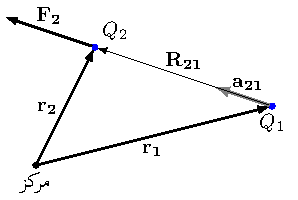
\includegraphics{figCoulombForceBetweenTwoCharges}
\caption{دو مثبت چارجوں کے مابین قوت دفع}
\label{شکل_سمتیہ_دو_مثبت_چارج_قوت_دفع}
\end{figure}
دونوں چارج مثبت یا دونوں چارج منفی ہونے کی صورت میں \عددیء{Q_2} پر مساوات \حوالہ{مساوات_کولومب_قوت_کی_مساوات_الف} سے قوت \سمتیہ{a_{21}} کی سمت میں حاصل ہوتا ہے۔یوں یکساں چارجوں کے مابین قوت دفع پایا جاتا ہے۔دو الٹ اقسام کے چارجوں کی صورت میں \عددیء{Q_2} پر قوت \سمتیہ{-a_{21}} کی سمت میں حاصل ہوتا ہے۔یوں الٹ اقسام کے چارجوں کے مابین قوت کشش پایا جاتا ہے۔  

\ابتدا{مثال}
شکل \حوالہ{شکل_سمتیہ_دو_مثبت_چارج_قوت_دفع} میں نقطہ \عددیء{A(3,2,4)} پر \عددیء{\SI{20}{\micro \coulomb}} کا چارج \عددیء{Q_1} جبکہ نقطہ \عددیء{B(1,5,9)} پر \عددیء{\SI{-50}{\coulomb}} کا چارج \عددیء{Q_2} پایا جاتا ہے۔منفی چارج \عددیء{Q_2} پر سمتی قوت حاصل کریں۔

حل:
\begin{align*}
\kvec{R_{21}}&=(1-3) \ax+(5-2) \ay+(9-4)\az\\
&=-2 \ax+3 \ay+5 \az\\
R_{21}&=\abs{\kvec{R_{21}}}=\sqrt{2^2+3^2+5^2}\\
&=\sqrt{38}\\
&=6.1644
\end{align*}
اور یوں
\begin{align*}
\kvec{a_{21}}&=\frac{{\kvec{R_{21}}}}{R_{21}}=\frac{-2 {\ax}+3 {\ay}+5 \az}{6.1644}\\
&=-0.324 \ax+0.487 \ay+0.811\az
\end{align*}
حاصل ہوتا ہے جس سے
\begin{align*}
\kvec{F_2}&=\frac{36 \pi  \times 10^9}{4 \pi} \frac{\left (-50\times 10^{-6} \times 20 \times 10^{-6} \right )}{38} \left(-0.324 \ax+0.487 \ay+0.811\az\right)\\
&=-0.237  \left(-0.324 \ax+0.487 \ay+0.811\az \right) \, \si{\newton}
\end{align*}
حاصل ہوتا ہے۔آپ دیکھ سکتے ہیں کہ قوت کی سمت \سمتیہ{a_{21}} کے الٹ سمت میں ہے۔یوں منفی چارج پر قوت کی سمت مثبت چارج کی جانب ہے یعنی اس پر قوت کشش پایا جاتا ہے۔
\انتہا{مثال}
%========================
کسی بھی چارج پر ایک سے زیادہ چارجوں سے پیدا مجموعی قوت تمام چارجوں سے پیدا علیحدہ علیحدہ قوتوں کا سمتی مجموعہ ہوتا ہے یعنی
\begin{align}
\kvec{F}=\sum_{i=1}^n \kvec{F}_i
\end{align}
اس حقیقت کو یوں بیان کیا جاتا ہے کہ کولومب کا قانون \اصطلاح{خطی}\فرہنگ{خطی}\حاشیہب{linear}\فرہنگ{linear} ہے۔ 

%========================
\حصہ{برقی میدان کی شدت}
نیوٹن کے کائناتی تجاذب کے قانون میں زمین کی کمیت کو \عددیء{M} لکھ کر کمیت \عددیء{m} پر قوت \عددیء{F} حاصل کی جا سکتی ہے۔ایک کلوگرام کمیت پر اس قوت کی مقدار \عددیء{\tfrac{F}{m}} ہو گی جسے \اصطلاح{زمین کی کشش}\فرہنگ{کشش!زمین}\حاشیہب{gravity}\فرہنگ{gravity} یا \اصطلاح{ثقلی اسراع} پکارا اور \عددیء{g} لکھا جاتا ہے۔زمین کی سطح پر \عددیء{g} کی مقدار تقریباً \عددیء{\SI{9.8}{\meter \per \second \squared}} کے برابر ہے۔
\begin{align}\label{مساوات_کولومب_زمین_کی_کشش}
g&=\frac{F}{m}=\frac{GM}{R^2}
\end{align}

کسی بھی کمیت \عددیء{M} کے گرد  \اصطلاح{تجاذبی میدان}\حاشیہب{gravitational field}\فرہنگ{تجاذبی میدان} پایا جاتا ہے۔ کسی بھی نقطے پر  اس تجاذبی میدن کو ناپنے کی خاطر اس نقطے پر پیمائشی کمیت \عددیء{m_p}\حاشیہد{\عددیء{m_p} لکھتے ہوئے  زیرنوشت میں \عددیء{p} لفظ پیمائشی  کے \موٹا{پ} کو ظاہر کرتا ہے، یعنی یہ وہ کمیت ہے جسے قوت  کی پیمائش کی خاطر استعمال کیا جا رہا ہے۔} رکھ کر اس پر قوت ناپی جاتی ہے۔مختلف مقامات پر اس طرح قوت ناپ کر ہم تجاذبی میدان کا جائزہ لے سکتے ہیں۔تجاذبی قوت کی مقدار کا دارومدار پیمائشی کمیت \حاشیہب{test mass} \عددیء{m_p} پر بھی منحصر ہے۔مختلف تجاذبی میدانوں کا آپس میں موازنہ کرتے وقت یہ ضروری ہے کہ تمام تجاذبی میدان جانچتے وقت ایک ہی قیمت کے پیمائشی کمیت استعمال کی جائے۔ماہرین طبیعیات عموماً \عددیء{m_p} کو ایک کلوگرام  رکھتے ہیں۔یہ ضروری نہیں کہ تجاذبی قوت ناپتے وقت ایک کلوگرام کی پیمائشی کمیت ہی استعمال کی جائے البتہ جوابات اکٹھے کرتے وقت \سمتیہ{F} کو \عددیء{m_p} سے تقسیم کرتے ہوئے ایک کلوگرام پر تجاذبی قوت حاصل کی جا سکتی ہے۔زمین کے قریب ایک کلو گرام کمیت پر قوت کشش کو ثقلی اسراع \عددی{g} پکارا جاتا ہے۔

\ابتدا{مثال}
زمین کی سطح پر دو سو گرام پیمائشی کمیت پر \عددیء{\SI{1.96}{\newton}} قوت ناپی جاتی ہے۔ثقلی اسراع حاصل کریں۔

حل:
\begin{align}
g=\frac{1.96}{0.2}=\SI{9.8}{\newton \per \kilogram}
\end{align}   
\انتہا{مثال}

مساوات \حوالہ{مساوات_کولومب_زمین_کی_کشش} سے ہم
\begin{gather}
\begin{aligned}
F&=m g\\
w&=m g
\end{aligned}
\end{gather}
لکھ سکتے ہیں جو زمین کی  سطح پر کمیت \عددیء{m} پر کشش ثقل \عددیء{F} دیتا ہے جسے  وزن پکارا اور  \عددیء{w} لکھا جاتا ہے۔
  
چارجوں پر بھی اسی طرح غور کیا جاتا ہے۔کسی بھی چارج \عددیء{Q} کے گرد برقی میدان پایا جاتا ہے۔اس برقی میدان میں چارج پر قوت اثر انداز ہوتا ہے۔چارج \عددیء{Q} کے برقی میدان کی شدت کے پیمائش کی خاطر اس میدان میں مختلف مقامات پر پیمائشی چارج \حاشیہب{test charge} \عددیء{q_p} پر قوت \سمتیہ{F} ناپ کر برقی میدان کا مطالعہ کیا جا سکتا ہے اور اس کا نقشہ بنایا جا سکتا ہے۔مختلف چارجوں کے برقی میدانوں کا آپس میں موازنہ کرتے وقت یہ ضروری ہے کہ تمام صورتوں میں ایک ہی قیمت کے پیمائشی چارج  استعمال کئے جائیں۔ماہرین طبیعیات \عددیء{q_p} کو ایک کولومب کا مثبت چارج  رکھتے ہیں۔یہ ضروری نہیں کہ قوت ناپتے وقت ایک کولومب کا مثبت پیمائشی چارج ہی استعمال کیا جائے البتہ جوابات اکٹھے کرتے وقت \سمتیہ{F} کو \عددیء{q_p} سے تقسیم کرتے ہوئے ایک مثبت کولومب پر قوت حاصل کی جاتی ہے جسے \اصطلاح{برقی میدان کی شدت}\فرہنگ{برقی میدان کی شدت}\حاشیہب{electric field intensity}\فرہنگ{electric field intensity} یا صرف \اصطلاح{برقی میدان} پکارا اور \سمتیہ{E} لکھا جاتا ہے یعنی
\begin{align}\label{مساوات_کولومب_برقی_شدت_اور_قوت}
\kvec{E}=\frac{\kvec{F}}{q_p}
\end{align}
مختلف مقامات پر موجود مختلف قیمتوں کے چارجوں سے کسی ایک نقطے پر  پیدا برقی میدان  تمام چارجوں کے مجموعی اثر سے پیدا ہو گا۔ایسا کولومب کے قانون کے خطی ہونے کی بنا پر ہوتا ہے۔کسی بھی نقطے پر \عددیء{n} چارجوں کا مجموعی \سمتیہ{E} تمام چارجوں کے علیحدہ علیحدہ پیدا کردہ  \سمتیازیرنوشت{E}{1}،  \سمتیازیرنوشت{E}{2}،\سمتیازیرنوشت{E}{3}،\عددیء{\cdots}  کا سمتی مجموعہ
\begin{align}
\kvec{E}=\sum_{i=1}^n \kvec{E}_i=\kvecsub{E}{1}+\kvecsub{E}{2}+\kvecsub{E}{3}+\cdots 
\end{align}
 ہوتا ہے۔یوں کسی بھی نقطے \عددیء{P}  پر \سمتیہ{E} ناپتے وقت اس نقطے پر ایک کولومب چارج \عددیء{q_p} رکھ کر اس چارج پر قوت ناپی جاتی ہے۔یہ قوت اس نقطے پر تمام چارجوں کا مجموعی  \سمتیہ{E} ہوتا ہے۔یاد رہے کہ کسی بھی نقطے پر  \سمتیہ{E} ناپتے وقت یہاں رکھے پیمائشی چارج \عددیء{q_p} کا اثر شامل نہیں ہوتا۔

مساوات  \حوالہ{مساوات_کولومب_قوت_کی_مساوات_الف} سے  چارج \عددیء{Q} سے \عددیء{\kvec{a}_R} سمت میں \عددیء{R} فاصلے پر برقی میدان کو
\begin{gather}
\begin{aligned}\label{مساوات_کولومب_قوت_کی_عمومی_مساوات}
\kvec{E}&=\frac{Q}{4 \pi \epsilon_0}\frac{\kvec{a_{R}}}{ R^2}\\
&=\frac{Q}{4 \pi \epsilon_0}\frac{\kvec{R}}{ R^3}
\end{aligned}
\end{gather}
لکھا جا سکتا ہے۔چارج کو کروی محدد کے مرکز پر تصور کرتے ہوئے اسی مساوات کو یوں لکھا جا سکتا ہے
\begin{align}\label{مساوات_کولومب_نقطہ_چارج_کروی_رداس_پر_تبدیل_نہیں_ہوتا}
\kvec{E}=\frac{Q}{4 \pi \epsilon_0 r^2} \ar
\end{align}
جہاں  \عددیء{\ar}  کروی محدد کا رداسی سمت میں اکائی سمتیہ ہے۔

نقطہ \عددیء{(x',y',z')} پر موجود چارج \عددیء{Q} سے نقطہ \عددیء{(x,y,z)} پر برقی شدت  یوں حاصل کی جا سکتی ہے۔
\begin{gather}
\begin{aligned} \label{مساوات_کولومب_نقطہ_چارج_سے_میدان_کا_حصول}
\kvec{E}&=\frac{1}{4 \pi \epsilon_0 }\frac{Q}{\abs{\kvec{r}-\kvec{r'}}^2} \frac{\kvec{r}-\kvec{r'}}{\abs{\kvec{r}-\kvec{r'}}}=\frac{Q}{4 \pi \epsilon_0 }\frac{\kvec{r}-\kvec{r'}}{\abs{\kvec{r}-\kvec{r'}}^3}\\
&=\frac{Q}{4 \pi \epsilon_0}\frac{\left[(x-x')\ax+(y-y')\ay+(z-z')\az\right]}{\left [(x-x')^2+(y-y')^2+(z-z')^2\right]^{\frac{3}{2}}}
\end{aligned}
\end{gather} 
جہاں
\begin{align*}
\kvec{r}&=x \ax+y \ay+z\az\\
\kvec{r'}&=x' \ax+y' \ay+z'\az\\
\kvec{R}&=\kvec{r}-\kvec{r'}=(x-x') \ax+(y-y') \ay+(z-z')\az
\end{align*}
کے برابر ہے۔
%===================
\ابتدا{مثال}\حاشیہط{چارج کم کرتے ہوئے جوابات 0 تا 1 کریں}
نقطہ \عددیء{N_1(4,1,1)} پر \عددیء{\SI{100}{\micro \coulomb}} کا چارج \عددیء{Q_1} جبکہ نقطہ \عددیء{N_2(1,4,2)} پر \عددیء{\SI{50}{\micro \coulomb}} کا چارج \عددیء{Q_2} پایا جاتا ہے۔نقطہ \عددیء{N_3(2,2,5)} پر  \عددیء{Q_1} سے پیدا \سمتیازیرنوشت{E}{1}  اور \عددیء{Q_2} سے پیدا \سمتیازیرنوشت{E}{2} حاصل کریں۔اس نقطے پر دونوں چارجوں کا مجموعی \عددیء{\kvec{E}} کیا ہو گا۔
\begin{figure}
\centering
\includegraphics[height=3.5cm]{figCoulombElectricFieldOfTwoCharges}
\caption{دو چارجوں سے پیدا برقی شدت}
\label{شکل_کولومب_دو_چارجوں_سے_پیدا_برقی_شدت}
\end{figure}

حل:شکل \حوالہ{شکل_کولومب_دو_چارجوں_سے_پیدا_برقی_شدت} میں صورت حال دکھایا گیا ہے۔پہلے \عددیء{Q_1} سے پیدا \سمتیازیرنوشت{E}{1} حاصل کرتے ہیں۔\عددیء{N_1}  سے \عددیء{N_3} تک سمتی فاصلہ
\begin{align*}
\kvecsub{R}{31}=\kvecsub{R}{3}-\kvecsub{R}{1}&=(2-4)\ax+(2-1)\ay+(5-1)\az\\
&=-2\ax+1\ay+4\az
\end{align*}
ہے جس سے
\begin{align*}
R_{31}&=\abs{\kvecsub{R}{31}}=\sqrt{2^2+1^2+4^2}\\
&=\sqrt{21}=4.583\\
\kvecsub{a}{31}&=\frac{\kvecsub{R}{31}}{R_{31}}=\frac{-2\ax+1\ay+4\az}{\sqrt{21}}\\
&=-0.436\ax+0.218\ay+0.873\az
\end{align*}
حاصل ہوتے ہیں۔یوں
\begin{align*}
\kvecsub{E}{1}&=9 \times 10^9 \frac{100 \times 10^{-6}}{21} \left(-0.436\ax+0.218\ay+0.873\az\right)\\
&=-\num{18686}\ax+\num{9343}\ay+\num{37414}\az \quad \si{\volt \per \meter}
\end{align*}
ہوتا ہے۔اسی طرح \عددیء{Q_2} کے لئے حل کرتے ہوئے
\begin{align*}
\kvecsub{R}{32}&=(2-1)\ax+(2-4)\ay+(5-2)\az\\
&=1\ax-2\ay+3\az
\end{align*}
اور
\begin{align*}
R_{32}&=\abs{\kvecsub{R}{32}}=\sqrt{1^2+2^2+3^2}=\sqrt{14}\\
\kvecsub{a}{32}&=\frac{1\ax-2\ay+3\az}{\sqrt{14}}\\
&=0.267\ax-0.535\ay+0.802\az
\end{align*}
سے
\begin{align*}
\kvecsub{E}{2}&=9 \times 10^9 \frac{50 \times 10^{-6}}{14} \left(0.267\ax-0.535\ay+0.802\az \right)\\
&=\num{8582}\ax-\num{17196}\ay+\num{25779}\az \quad \si{\volt \per \meter}
\end{align*}
ملتا ہے۔ان دو جوابات کا سمتی مجموعہ لیتے ہوئے کُل \kvec{E} حاصل کرتے ہیں۔
\begin{align*}
\kvec{E}&=\kvecsub{E}{1}+\kvecsub{E}{2}\\
&=\left(\num{-18686} \ax+\num{9343} \ay+\num{37414}\az\right)+\left(\num{8582}\ax-\num{17196}\ay+\num{25779}\az\right)\\
&=-\num{10104}\ax-\num{7853}\ay+\num{63193}\az \quad \si{\volt \per \meter}
\end{align*} 
\انتہا{مثال}
%===================
 
مساوات \حوالہ{مساوات_کولومب_برقی_شدت_اور_قوت} کو
\begin{align}
\kvec{F}=q \kvec{E}
\end{align}
لکھا جا سکتا ہے جو برقی میدان \سمتیہ{E} کے موجودگی میں چارج \عددیء{q} پر قوت \سمتیہ{F} دیتا ہے۔


\حصہ{یکساں چارج بردار سیدھی لامحدود لکیر  کا برقی میدان}
شکل \حوالہ{شکل_کولومب_لامحدود_لکیر_پر_چارج_کا_میدان} میں \عددیء{z} محدد پر \عددیء{z=-\infty} سے \عددیء{z=+\infty} تک یکساں چارج کی کثافت پائی جاتی ہے۔آپ تصور کر سکتے ہیں کہ \عددیء{z} محدد پر انتہائی قریب قریب برابر فاصلے پر یکساں \اصطلاح{نقطہ چارج} رکھے گئے ہیں۔یوں اگر \عددیء{\Delta L} لمبائی میں کُل \عددیء{\Delta Q} چارج پایا جائے تب اکائی لمبائی میں \عددیء{\tfrac{\Delta Q}{\Delta L}} چارج پایا جائے گا جسے \اصطلاح{لکیری چارج کثافت}\فرہنگ{کثافت!لکیری چارج}\حاشیہب{line charge density}\فرہنگ{density!line charge}  \عددیء{\rho_L}\حاشیہد{اس کتاب میں رداس کے لئے بھی \عددیء{\rho} استعمال کیا جاتا ہے۔\عددیء{\rho} کو جب بھی کثافت کے لئے استعمال کیا جائے،اس کے زیر نوشت میں \تحریر{L}، \تحریر{S} یا \تحریر{h} لکھا جائے گا۔} کہا جاتا ہے اور جس کی اکائی \عددیء{\si{\coulomb / \meter}} ہے۔لکیری چارج کثافت کی تعریف
\begin{align}
\rho_L=\lim_{\Delta L \to 0}\frac{\Delta Q}{\Delta L}
\end{align}
ہے۔لکیر پر چھوٹی لمبائی  اتنی کم نہیں کی جاتی کہ چارج بردار الیکٹران علیحدہ علیحدہ نظر آئیں اور لکیری کثافت کی جگہ نقطہ چارج نظر آئیں۔اگر لکیر پر چارج کی تقسیم ہر جگہ یکساں نہ ہو تب لکیری چارج کثافت متغیر ہو گی۔آئیں یکساں لکیری چارج کثافت سے خالی خلاء میں پیدا برقی میدان پر غور کریں۔ 
 \begin{figure}
\centering
\includegraphics[height=3.5cm]{figCoulombElectricFieldOfInfiniteLineCharge}
\caption{یکساں چارج بردار سیدھی لامحدود لکیر  کا برقی میدان}
\label{شکل_کولومب_لامحدود_لکیر_پر_چارج_کا_میدان}
\end{figure}

پہلے بغیر قلم اٹھائے اس مسئلے کی نوعیت پر توجہ دیتے ہیں۔مقام \عددیء{(0,0,z)} پر  چھوٹی سی لمبائی \عددیء{\Delta z} میں \عددیء{\rho_L \Delta z} چارج پایا جاتا ہے جسے نقطہ چارج تصور کرتے ہوئے آگے بڑھتے ہیں۔\عددیء{z} محدد کے گرد \عددیء{z=0} یعنی  \عددیء{xy} سطح پر  شکل \حوالہ{شکل_کولومب_لامحدود_لکیر_پر_چارج_کا_میدان} میں نقطہ دار گول دائرہ بنایا گیا ہے۔نقطہ چارج \عددیء{\rho_L \Delta z} سے دائرے پر کسی بھی مقام پر پیدا برقی میدان پر غور کرتے ہیں۔برقی میدان کی مقدار کا دارومدار میدان پیدا کرنے والے چارج اور چارج سے فاصلے پر ہے۔نقطہ دار لکیر پر پائے جانے والے تمام نقطوں کا \عددیء{(0,0,z)} سے فاصلہ برابر ہے۔یوں ہم توقع کرتے ہیں کہ اس دائرے پر برقی میدان کی شدت کی حتمی قیمت ہر جگہ برابر ہو گی۔اس کو یوں بھی بیان کیا جا سکتا ہے کہ چارج کی نقطہ نظر سے نقطہ دار لکیر پر تمام نقطے بالکل یکساں نظر آتے ہیں۔اس مشابہت سے ہم کہہ سکتے ہیں کہ نقطہ دار دائرے پر ہر جگہ برقی میدان یکساں ہو گا۔ 

آئیں شکل \حوالہ{شکل_کولومب_لامحدود_لکیر_پر_چارج_کا_میدان} کو دیکھتے ہوئے  ایک اور مشابہت پر غور کرتے ہیں۔چونکہ \سمتیہ{E} سمتی فاصلہ \سمتیہ{R} کی سمت میں ہوتا ہے لہٰذا دائرے پر کسی بھی نقطے پر نقطہ چارج \عددیء{\rho_L \Delta z} سے پیدا  \عددیء{\kvec{E}} کے دو اجزاء پائے جائیں گے یعنی
\begin{align}
\kvec{E}=\kvec{E}_\rho+\kvec{E}_z
\end{align}
مثبت \عددیء{\rho_L} کی صورت میں \عددیء{(0,0,z)} پر موجود چارج سے  \عددیء{\kvec{E}_z} کی سمت منفی  \عددیء{z} جانب ہو گی۔اسی طرح \عددیء{(0,0,-z)} پر پائے جانے والے مثبت چارج سے دائرے پر پیدا \عددیء{\kvec{E}} کی سمت مثبت \عددیء{z} جانب ہو گی۔دائرے پر یہ دونوں ارکان ایک دونوں کو ختم کریں گے۔اسی عمل سے دائرے پر کسی بھی نقطے پر مثبت \عددیء{z} محدد پر کسی  بھی  فاصلے پر پائے جانے والے چارج سے پیدا \عددیء{\kvec{E}_z} کے اثر کو منفی \عددیء{z} محدد پر اتنے ہی فاصلے پر چارج سے پیدا  \عددیء{\kvec{E}_z} ختم کرتا ہے۔یوں دائرے پر
\begin{align}\label{مساوات_کولومب_لامحدود_چارج_رداس_کا_میدان_صفر}
\kvec{E}_z=0
\end{align}
ہو گا۔

ایک آخری مشابہت پر اب غور کرتے ہیں۔اگر نقطہ دار دائرے کو \عددیء{z} محدد پر مثبت یا منفی جانب  لے جایا جائے تو کیا ہو گا؟ اب بھی دائرے  کے ایک جانب کسی بھی فاصلے پر چارج کا اثر دائرے کے دوسری جانب اتنے ہی فاصلے پر چارج ختم کرے گا۔یوں دائرے کے ایک جانب یعنی \عددیء{z} محدد پر \عددیء{\infty} تک فاصلے پر چارجوں کے \عددیء{\kvec{E}_z} کو دائرے کی دوسری جانب \عددیء{z} محدد پر \عددیء{-\infty} تک فاصلے پر چارجوں کا \عددیء{\kvec{E}_z} ختم کرے گا اور یوں خلاء میں  ہر جگہ مساوات \حوالہ{مساوات_کولومب_لامحدود_چارج_رداس_کا_میدان_صفر} درست ثابت ہوتا ہے۔اس حقیقت کو یوں بہتر بیان کیا جا سکتا ہے کہ  لامحدود لکیر پر یکساں کثافت چارج  سے خلاء میں برقی میدان صرف رداس کی سمت میں پیدا ہو گا۔آئیں  اس \سمتیہ{E} کو حاصل کریں۔

شکل \حوالہ{شکل_کولومب_لامحدود_لکیر_پر_چارج_کا_میدان} میں مقام \عددیء{z} پر نقطہ چارج \عددیء{\rho_L \Delta z}  دائرے پر \عددیء{\Delta \kvec{E}} پیدا کرتا ہے۔محدد کے مرکز سے نقطہ چارج کا مقام سمتیہ \عددیء{z \az} سے ظاہر کیا جا سکتا ہے جبکہ دائرے پر کسی بھی نقطے \عددیء{N} کو سمتیہ \عددیء{\rho \arho} ظاہر کرتا ہے۔یوں نقطہ چارج سے  \عددیء{N} تک کا سمتی فاصلہ اور اسی سمت میں اکائی سمتیہ یوں حاصل کئے جائیں گے۔
\begin{align*}
\kvec{R}&=\rho \arho-z\az\\
\abs{\kvec{R}}&=R=\sqrt{\rho^2+z^2}\\
\kvec{a}_R&=\frac{\kvec{R}}{\abs{\kvec{R}}}=\frac{\rho \arho-z\az}{\sqrt{\rho^2+z^2}}
\end{align*}
مساوات \حوالہ{مساوات_کولومب_نقطہ_چارج_کروی_رداس_پر_تبدیل_نہیں_ہوتا} سے
\begin{align*}
\Delta \kvec{E}&=\frac{\rho_L \Delta z}{4 \pi \epsilon_0 \left(\rho^2+z^2 \right)} \frac{\rho \arho-z\az}{\sqrt{\rho^2+z^2}}\\
&=\frac{\rho_L \Delta z \left(\rho \arho-z\az \right)}{4 \pi \epsilon_0\left(\rho^2+z^2 \right)^{\frac{3}{2}}}
\end{align*}
حاصل ہوتا ہے۔تمام چارجوں کے اثرات کو یکجا کرنے کی خاطر مندرجہ بالا مساوات کو تکمل کی شکل دے کر مندرجہ ذیل مساوات میں دکھایا گیا ہے۔تکملہ کے حدود \عددیء{-\infty} اور \عددیء{+\infty}  ہیں۔
\begin{align}
\kvec{E}=\int \dif  \kvec{E}=\int\limits_{-\infty}^{+\infty} \left[\frac{\rho_L \left(\rho \arho-z\az \right)}{4 \pi \epsilon_0\left(\rho^2+z^2 \right)^{\frac{3}{2}}}\right] \dif z
\end{align}
اس تکمل کو یوں لکھا جا سکتا ہے
\begin{align}\label{مساوات_کولومب_لامحدود_لکیر_چارج_کا_میدان}
\kvec{E}&=\frac{\rho_L \rho \arho}{4 \pi \epsilon_0}\int\limits_{-\infty}^{+\infty} \frac{\dif z }{\left(\rho^2+z^2 \right)^{\frac{3}{2}}} -\frac{\rho_L \az}{4 \pi \epsilon_0}\int\limits_{-\infty}^{+\infty} \frac{z \dif z}{\left(\rho^2+z^2 \right)^{\frac{3}{2}}}
\end{align}
جہاں مساوات کی نشان کے دائیں جانب پہلا تکمل  \Erho اور دوسرا تکمل \Ez دیتا ہے  یعنی
\begin{gather}
\begin{aligned}\label{مساوات_کولومب_رداسی_اور_عمودی_برقی_میدان}
\Erho&=\frac{\rho_L \rho \arho}{4 \pi \epsilon_0}\int\limits_{-\infty}^{+\infty} \frac{\dif z }{\left(\rho^2+z^2 \right)^{\frac{3}{2}}}\\
\Ez&=-\frac{\rho_L \az}{4 \pi \epsilon_0}\int\limits_{-\infty}^{+\infty} \frac{z \dif z}{\left(\rho^2+z^2 \right)^{\frac{3}{2}}}
\end{aligned}
\end{gather}

مساوات \حوالہ{مساوات_کولومب_لامحدود_چارج_رداس_کا_میدان_صفر} کی مدد سے ہم دیکھ سکتے ہیں کہ دوسرا تکملہ صفر جواب دیگا۔آئیں دونوں تکمل کو باری باری حل کریں۔پہلے \Erho حل کرتے ہیں۔اس مساوات میں
\begin{align*}
z=\rho \tan \alpha
\end{align*}
استعمال کرتے ہیں۔ایسا کرتے ہوئے تکمل کا ابتدائی حد 
\begin{align*}
-\infty &= \rho \tan \alpha_{\textrm{ابتدائی}}\\
\alpha_{\textrm{ابتدائی}} &= -\frac{\pi}{2}
\end{align*}
اور اختتامی حد
\begin{align*}
\infty &= \rho \tan \alpha_{\textrm{اختتامی}}\\
\alpha_{\textrm{اختتامی}} &= \frac{\pi}{2}
\end{align*}
حاصل ہوتے ہیں۔مزید
\begin{align*}
\dif z=\rho \sec^2 \alpha \dif \alpha
\end{align*}
لکھا جائے گا۔یوں
\begin{align*}
\Erho&=\frac{\rho_L \rho \arho}{4 \pi \epsilon_0}\int\limits_{-\frac{\pi}{2}}^{+\frac{\pi}{2}} \frac{\rho \sec^2 \alpha \dif \alpha}{\left(\rho^2+\rho^2 \tan^2 \alpha \right)^{\frac{3}{2}}}\\
&=\frac{\rho_L \rho \arho}{4 \pi \epsilon_0}\int\limits_{-\frac{\pi}{2}}^{+\frac{\pi}{2}} \frac{\rho \sec^2 \alpha \dif \alpha}{\rho^3 \left(1+ \tan^2 \alpha \right)^{\frac{3}{2}}}
\end{align*}
لکھا جائے گا جس میں
\begin{align*}
1+\tan^2 \alpha=\sec^2 \alpha
\end{align*}
استعمال کرتے ہوئے
\begin{gather}
\begin{aligned}\label{مساوات_کولومب_لامحدود_لکیر_رداسی_میدان}
\Erho&=\frac{\rho_L \rho \arho}{4 \pi \epsilon_0}\int\limits_{-\frac{\pi}{2}}^{+\frac{\pi}{2}} \frac{\rho \sec^2 \alpha \dif \alpha}{\rho^3 \sec^3 \alpha}\\
&=\frac{\rho_L  \arho}{4 \pi \epsilon_0 \rho}\int\limits_{-\frac{\pi}{2}}^{+\frac{\pi}{2}} \cos \alpha \dif \alpha\\
&=\frac{\rho_L  \arho}{4 \pi \epsilon_0 \rho} \eval{\sin \alpha}_{-\frac{\pi}{2}}^{\frac{+\pi}{2}}\\
&=\frac{\rho_L }{2 \pi \epsilon_0 \rho} \arho
\end{aligned}
\end{gather}
ملتا ہے جہاں دوسری  قدم پر \عددیء{\sec \alpha=\tfrac{1}{\cos \alpha}} کا استعمال کیا گیا۔

آئیں اب مساوات \حوالہ{مساوات_کولومب_رداسی_اور_عمودی_برقی_میدان} کے   دوسرے جزو کو حل کریں۔اس میں بھی \عددیء{z= \rho \tan \alpha} استعمال کرتے ہیں۔یوں
\begin{align*}
\Ez&=-\frac{\rho_L \az}{4 \pi \epsilon_0}\int\limits_{-\infty}^{+\infty} \frac{z \dif z}{\left(\rho^2+z^2 \right)^{\frac{3}{2}}}\\
&=-\frac{\rho_L \az}{4 \pi \epsilon_0}\int\limits_{-\frac{\pi}{2}}^{+\frac{\pi}{2}} \frac{\rho^2 \tan \alpha  \sec^2 \alpha \dif \alpha}{\left(\rho^2+\rho^2 \tan^2 \alpha \right)^{\frac{3}{2}}}\\
&=-\frac{\rho_L \az}{4 \pi \epsilon_0 \rho}\int\limits_{-\frac{\pi}{2}}^{+\frac{\pi}{2}} \frac{ \tan \alpha  \sec^2 \alpha \dif \alpha}{\left(1+ \tan^2 \alpha \right)^{\frac{3}{2}}}
\end{align*}
سے
\begin{gather}
\begin{aligned}\label{مساوات_کولومب_لامحدود_لکیر_عمودی_میدان}
\Ez&=-\frac{\rho_L \az}{4 \pi \epsilon_0 \rho}\int\limits_{-\frac{\pi}{2}}^{+\frac{\pi}{2}} \frac{ \tan \alpha  \sec^2 \alpha \dif \alpha}{\sec^3 \alpha}\\
&=-\frac{\rho_L \az}{4 \pi \epsilon_0 \rho}\int\limits_{-\frac{\pi}{2}}^{+\frac{\pi}{2}} \sin \alpha \dif \alpha\\
&=\frac{\rho_L \az}{4 \pi \epsilon_0 \rho} \eval{\cos \alpha}_{-\frac{\pi}{2}}^{+\frac{\pi}{2}}\\
&=0
\end{aligned}
\end{gather}
ملتا ہے۔یہی جواب مساوات \حوالہ{مساوات_کولومب_لامحدود_چارج_رداس_کا_میدان_صفر} میں حاصل کیا گیا تھا۔

مساوات \حوالہ{مساوات_کولومب_لامحدود_لکیر_رداسی_میدان} اور مساوات \حوالہ{مساوات_کولومب_لامحدود_لکیر_عمودی_میدان} سے مساوات \حوالہ{مساوات_کولومب_لامحدود_لکیر_چارج_کا_میدان}  کا حل یوں لکھا جائے گا
\begin{align}\label{مساوات_کولومب_لامحدود_لکیر_رداسی_میدان_پیدا_کرتا_ہے}
\kvec{E}=\Erho=\frac{\rho_L }{2 \pi \epsilon_0 \rho} \arho
\end{align}
جس کے مطابق لامحدود سیدھی لکیر پر یکساں چارج سے برقی میدان رداس \عددیء{\rho}  کے بالعکس متناسب ہے۔اس نتیجے  کا مساوات \حوالہ{مساوات_کولومب_نقطہ_چارج_کروی_رداس_پر_تبدیل_نہیں_ہوتا} کے ساتھ موازنہ کریں جو نقطہ چارج کی برقی میدان بیان کرتا ہے۔نقطہ چارج کا برقی میدان کروی رداس کے مربع کے بالعکس متناسب ہے۔یوں اگر لامحدود لکیر کے چارج سے فاصلہ دگنا کر دیا جائے تو برقی میدان آدھا ہو جائے گا جبکہ نقطہ چارج سے فاصلہ دگنا کرنے سے برقی میدان چار گنا کم ہوتا ہے۔

کسی بھی سمت میں لامحدود سیدھی لکیر پر چارج کا برقی میدان مساوات \حوالہ{مساوات_کولومب_لامحدود_لکیر_رداسی_میدان_پیدا_کرتا_ہے} میں بیان خوبیوں پر پورا اترے گا۔ایسی صورت میں کسی بھی نقطے پر \سمتیہ{E} حاصل کرنے کی خاطر اس نقطے سے چارج کے لکیر تک کم سے کم فاصلہ \عددیء{R} حاصل کریں۔یہ فاصلہ نقطے سے لکیر پر عمود کھینچنے سے حاصل ہو گا۔اس فاصلے کو \عددیء{\rho} تصور کریں۔لکیر سے عمودی سمت میں نقطے کی جانب اکائی سمتیہ \عددیء{\kvec{a}_R} کو \arho   \, تصور کریں۔ایسی صورت میں مساوات \حوالہ{مساوات_کولومب_لامحدود_لکیر_رداسی_میدان_پیدا_کرتا_ہے} کو
\begin{align}\label{مساوات_کولومب_کسی_بھِی_سمت_میں_لامحدود_لکیر_رداسی_میدان_پیدا_کرتا_ہے}
\kvec{E}=\frac{\rho_L }{2 \pi \epsilon_0 R} \kvec{a}_R
\end{align}
لکھ سکتے ہیں۔
%===================
\ابتدا{مثال}
\عددیء{y} محدد کے  متوازی اور \عددیء{(x,0,0)} سے گزرتی لامحدود لکیر پر \عددیء{\rho_L} کثافت کا چارج پایا جاتا ہے۔نقطہ \عددیء{(x',y',z')} پر \سمتیہ{E} حاصل کریں۔
\begin{figure}
\centering
\includegraphics[height=3.5cm]{figCoulombElectricFieldOfInfiniteLineChargeAlongYaxis}
\caption{کسی بھی سمت میں لامحدود لکیر پر چارج کی مثال}
\label{شکل_کولومب_کسی_بھی_سمت_لامحدود_لکیر_پر_چارج_کا_میدان}
\end{figure}

حل:شکل \حوالہ{شکل_کولومب_کسی_بھی_سمت_لامحدود_لکیر_پر_چارج_کا_میدان} میں صورت حال دکھایا گیا ہے۔\عددیء{(x',y',z')} سے چارج کے لکیر پر عمود \عددیء{(x,y',0)} پر ٹکراتا ہے۔ان دو نقطوں کا آپس میں فاصلہ \عددیء{\sqrt{(x'-x)^2+z^2}} ہے جبکہ 
\begin{align*}
\kvec{R}&=(x'-x)\ax+z\az\\
\kvec{a}_R&=\frac{(x'-x)\ax+z\az}{\sqrt{(x'-x)^2+z^2}}
\end{align*}
ہیں۔یوں
\begin{align*}
\kvec{E}=\frac{\rho_L}{2 \pi \epsilon_0 \sqrt{(x'-x)^2+z^2}} \kvec{a}_R
\end{align*}
ہو گا۔
\انتہا{مثال}
%================================
\ابتدا{مشق}
\عددیء{y} محدد پر \عددیء{-\infty} سے \عددیء{+\infty} تک \عددیء{\SI{10}{\nano \coulomb \per \meter}} چارج کی کثافت پائی جاتی ہے۔ نقطہ \عددیء{N_1(0,0,6)} اور نقطہ  \عددیء{N_2(0,8,6)}  پر \سمتیہ{E} حاصل کریں۔

جواب: دونوں نقطوں پر \عددی{\kvec{E}=30 \az} کے برابر ہے۔
\انتہا{مشق}
%====================

\ابتدا{مشق}
\عددیء{x} محدد پر \عددیء{-\infty} سے \عددیء{+\infty} تک \عددیء{\SI{5}{\nano \coulomb \per \meter}} چارج کی کثافت پائی جاتی ہے۔ نقطہ \عددیء{N_1(0,5,0)} اور نقطہ
  \عددیء{N_2(7,3,4)}  پر \سمتیہ{E} حاصل کریں۔

جوابات:\عددیء{\kvec{E}_1=18 \az \, \si{\volt \per \meter}} اور \عددیء{ \kvec{E}_2=18 \left(\frac{3\ay+4\az}{5}\right) \,\si{\volt \per \meter}}

\انتہا{مشق}
%=======================
\حصہ{یکساں چارج بردار ہموار لامحدود سطح}
شکل \حوالہ{شکل_کولومب_لامحدود_سطح_پر_چارج} میں  \عددیء{z=0} پر لامحدود \عددیء{x-y} سطح دکھائی گئی ہے۔تصور کریں کہ اس پوری  سطح پر انتہائی قریب قریب نقطہ چارج یوں رکھے گئے ہیں کہ سطح پر کہیں بھی چھوٹی رقبہ \عددیء{\Delta S} پر  یکساں قیمت کا چارج \عددیء{\Delta Q} پایا جاتا ہے۔اس طرح اکائی رقبے پر کل \عددیء{\tfrac{\Delta Q}{\Delta S}} چارج پایا جائے گا جسے \اصطلاح{سطحی چارج  کثافت}\فرہنگ{کثافت!سطحی  چارج}\حاشیہب{surface charge density}\فرہنگ{density!surface charge} \عددیء{\rho_S} کہتے ہیں۔سطحی چارج کثافت کی تعریف
\begin{align}\label{مساوات_کولومب_سطحی_کثافت_تعریف}
\rho_S=\lim_{\Delta S \to 0}\frac{\Delta Q}{\Delta S}
\end{align}
ہے۔چھوٹی سطح اتنی کم نہیں لی جاتی کہ اس پر چارج بردار الیکٹران علیحدہ علیحدہ بطور نقطہ چارج نظر آئیں بلکہ اسے اتنا رکھا جاتا ہے کہ علیحدہ علیحدہ الیکٹران کا اثر قابل نظر انداز ہو۔ سطح پر ہر جگہ چارج کا تقسیم یکساں نہ ہونے کی صورت میں \عددیء{\rho_S} کی قیمت متغیر ہو گی۔آئیں لامحدود سطح پر یکساں چارج کثافت سے خالی خلاء میں  پیدا \سمتیہ{E} حاصل کریں۔

پہلے غور کرتے ہیں کہ آیا مختلف مقامات سے  دیکھتے ہوئے کچھ اخذ کرنا ممکن ہے۔اگر اس چارج بردار سطح کے سامنے ہم کھڑے ہو جائیں تو ہمیں سامنے لامحدود چارج بردار سطح نظر آئے گی۔سطح سے برابر فاصلے پر ہم جہاں بھی جائیں ہمیں صورت حال میں کوئی تبدیلی نظر نہیں آئے گی۔اسی طرح اگر ہم سطح کی دوسری طرف اتنے ہی فاصلے پر چلے جائیں تو ہمیں صورت حال میں کسی قسم کی کوئی تبدیلی نظر نہیں آئے گی۔اس مشابہت سے ہم کہہ سکتے ہیں کہ ایسی سطح سے برابر فاصلے پر تمام نقطوں  پر یکساں برقی میدان پایا جائے گا۔اس کے برعکس اگر ہم اس سطح سے دور ہو جائیں تو ہمیں سطح قدر دور نظر آئے گی اور ہو سکتا ہے کہ اس تبدیلی سے \سمتیہ{E} پر اثر ہو۔آئیں اب مسئلے کو حساب و کتاب سے حل کرتے ہوئے \سمتیہ{E} حاصل کریں۔
\begin{figure}
\centering
\includegraphics[height=3.5cm]{figCoulombElectricFieldOfInfiniteSurfaceCharge}
\caption{یکساں چارج بردار ہموار لامحدود سطح}
\label{شکل_کولومب_لامحدود_سطح_پر_چارج}
\end{figure}

شکل \حوالہ{شکل_کولومب_لامحدود_سطح_پر_چارج}  میں چارج بردار سطح پر  \عددیء{z} محدد کے متوازی دو انتہائی قریب قریب لکیریں کھینچی گئی ہیں جن کے مابین فاصلہ \عددیء{\dif y} ہے۔اس گھیرے گئے رقبے کی چوڑائی \عددیء{\dif y} ہے۔یوں \عددیء{\Delta L} لمبائی اور \عددیء{\dif y} چوڑائی رقبے میں \عددیء{\rho_S \Delta L \dif y} چارج پایا جائے گا۔لکیروں سے گھیرے رقبے کو چارج کی سیدھی لکیر تصور کیا جا سکتا ہے جس پر اکائی لمبائی کے رقبے پر \عددیء{\tfrac{\rho_S \Delta L \dif y}{\Delta L}} چارج پایا جائے گا جسے \عددیء{\rho_L} تصور کیا جا سکتا ہے یعنی
\begin{align}
\rho_L=\rho_S \dif y
\end{align}

لامحدود لکیر پر یکساں چارج کی کثافت سے پیدا برقی میدان پر گزشتہ حصے میں غور کیا گیا۔نقطہ \عددیء{(x,0,0)}  پر \سمتیہ{E} حاصل کرتے ہیں۔شکل میں لامحدود چارج کی لکیر سے اس نقطے تک کا قریبی سمتی فاصلہ \سمتیہ{R} دکھایا گیا ہے جہاں
\begin{align}
\kvec{R}=x \ax-y\ay
\end{align}
کے برابر ہے جس سے
\begin{gather}
\begin{aligned}
R&=\abs{\kvec{R}}=\sqrt{x^2+y^2}\\
\kvec{a}_R&=\frac{x\ax-y\ay}{\sqrt{x^2+y^2}}
\end{aligned}
\end{gather}
حاصل ہوتے ہیں۔یوں چارج بردار لکیر سے \عددیء{(x,0,0)} پر پیدا برقی میدان کو مساوات \حوالہ{مساوات_کولومب_کسی_بھِی_سمت_میں_لامحدود_لکیر_رداسی_میدان_پیدا_کرتا_ہے}  کی مدد سے
\begin{gather}
\begin{aligned}
\dif \kvec{E} &= \frac{\rho_S \dif y}{2 \pi \epsilon_0 \sqrt{x^2+y^2}} \frac{x\ax-y\ay}{\sqrt{x^2+y^2}}\\
&=\frac{\rho_S \dif y \left(x\ax-y\ay \right)}{2 \pi \epsilon_0 \left(x^2+y^2\right)}
\end{aligned}
\end{gather}
لکھا جا سکتا ہے۔اس جواب کو \عددیء{\dif \kvec{E}=\dif \kvec{E}_x+\dif \kvec{E}_y} لکھا جا سکتا ہے جہاں
\begin{gather}\label{مساوات_کولومب_لامحدود_سطح_کی_میدان_کے_اجزاء}
\begin{aligned}
\dif \kvec{E}_x&=\frac{\rho_S x \dif y }{2 \pi \epsilon_0 \left(x^2+y^2\right)}\ax\\
\dif \kvec{E}_y&=-\frac{\rho_S y\dif y }{2 \pi \epsilon_0 \left(x^2+y^2\right)} \ay
\end{aligned}
\end{gather}
کے برابر ہیں۔\عددیء{x} محدد کے ایک جانب چارج بردار لکیر مندرجہ بالا برقی میدان پیدا کرتا ہے۔غور کرنے سے معلوم ہوتا ہے کہ \عددیء{x} محدد کے دوسری جانب اتنے ہی فاصلے پر چارج بردار لکیر سے پیدا برقی میدان مندرجہ بالا \عددیء{\dif \kvec{E}_y} کو ختم کرے گا۔یوں کسی بھی مثبت \عددیء{y} پر کھینچی لکیر کے \عددیء{\dif \kvec{E}_y}  کو منفی \عددیء{y} پر کھینچی لکیر کا \عددیء{\dif \kvec{E}_y} ختم کرے گا۔\عددیء{x} محدد کے دونوں جانب مسئلے کی مشابہت سے یوں ہم توقع کرتے ہیں کہ
\begin{align}\label{مساوات_کولومب_سطحی_صفر_شدت_حصہ}
\kvec{E}_y=0
\end{align} 
ہو گا۔

آئیں اب حساب و کتاب سے مساوات \حوالہ{مساوات_کولومب_لامحدود_سطح_کی_میدان_کے_اجزاء} کو حل کریں۔پہلے \عددیء{\kvec{E}_x} حاصل کرتے ہیں۔مساوات \حوالہ{مساوات_کولومب_لامحدود_سطح_کی_میدان_کے_اجزاء} میں دئے \عددیء{\dif \kvec{E}_x} کا تکمل لیتے ہیں۔ایسا کرنے کی خاطر
\begin{gather}
\begin{aligned}\label{مساوات_کولومب_ٹینجنٹ_کی_مدد_سے_تکملہ_کا_حصول}
y&=x \tan \alpha\\
\dif y &=x \sec^2 \alpha \dif \alpha
\end{aligned}
\end{gather}
کا استعمال کرتے ہیں۔شکل \حوالہ{شکل_کولومب_لامحدود_سطح_پر_چارج} میں \عددیء{\alpha} کی نشاندہی کی گئی ہے۔یوں
\begin{align*}
\kvec{E}_x=\int \dif \kvec{E}_x &=\frac{\rho_S x \ax}{2\pi \epsilon_0}\int_{y=-\infty}^{y=+\infty}\frac{\dif y }{ \left(x^2+y^2\right)}\\
&=\frac{\rho_S x \ax}{2\pi \epsilon_0}\int_{\alpha=-\frac{\pi}{2}}^{\alpha=+\frac{\pi}{2}} \frac{x \sec^2 \alpha \dif \alpha}{x^2\left(1+ \tan^2 \alpha\right)}
\end{align*}
میں \عددیء{\sec^2  \alpha=1+\tan^2 \alpha} کے استعمال سے
\begin{gather}
\begin{aligned}\label{مساوات_کولومب_لامحدود_سطح_عمودی_جزو}
\kvec{E}_x&=\frac{\rho_S\ax}{2\pi \epsilon_0}\int_{\alpha=-\frac{\pi}{2}}^{\alpha=+\frac{\pi}{2}}\dif \alpha\\
&=\frac{\rho_S\ax}{2\pi \epsilon_0} \eval{\alpha}_{-\frac{\pi}{2}}^{+\frac{\pi}{2}}\\
&=\frac{\rho_S}{2 \epsilon_0}\ax
\end{aligned}
\end{gather}
حاصل ہوتا ہے۔آئیں اب \عددیء{\kvec{E}_y} حاصل کریں۔

مساوات \حوالہ{مساوات_کولومب_لامحدود_سطح_کی_میدان_کے_اجزاء} میں دئے \عددیء{\dif \kvec{E}_y} کا تکمل لیتے ہیں۔
\begin{align*}
\kvec{E}_y=\int \dif \kvec{E}_y&=-\frac{\rho_S \ay}{2 \pi \epsilon_0} \int_{y=-\infty}^{y=+\infty}\frac{ y\dif y }{ \left(x^2+y^2\right)}
\end{align*}
تکمل کے نشان کے اندر \عددیء{f(y)=x^2+y^2} لیتے ہوئے  اسے \عددیء{\tfrac{\dif f(y)}{2 f(y)}} لکھا جا سکتا ہے جس کا تکمل \عددیء{\tfrac{\ln f(y)}{2}} ہے۔یوں
\begin{gather}
\begin{aligned}\label{مساوات_کولومب_لامحدود_سطح_افقی_جزو}
\kvec{E}_y&=-\frac{\rho_S \ay}{2 \pi \epsilon_0} \eval{\frac{\ln(x^2+y^2)}{2}}_{y=-\infty}^{y=+\infty}\\
&=0
\end{aligned}
\end{gather}
حاصل ہوتا ہے۔مساوات \حوالہ{مساوات_کولومب_سطحی_صفر_شدت_حصہ} میں یہی جواب حاصل کیا گیا تھا۔

مساوات \حوالہ{مساوات_کولومب_لامحدود_سطح_عمودی_جزو} اور مساوات \حوالہ{مساوات_کولومب_لامحدود_سطح_افقی_جزو} کی مدد سے یکساں چارج بردار لامحدود سطح کی برقی میدان
\begin{align}\label{مساوات_کولومب_لامحدود_سطح_کی_برقی-میدان}
\kvec{E}=\frac{\rho_S}{2 \epsilon_0}\kvec{a}_N
\end{align}
لکھی جا سکتی ہے جہاں \عددیء{\kvec{a}_N} اس سطح کا عمودی اکائی سمتیہ ہے۔آپ دیکھ سکتے ہیں کہ سطح سے فاصلہ کم یا زیادہ کرنے سے برقی میدان کی شدت پر کوئی اثر نہیں ہوتا۔سطح کے دونوں جانب برقی میدان اسی مساوات سے حاصل کی جائے گی۔ظاہر ہے کہ سطح کے دونوں جانب کے اکائی عمودی سمتیہ آپس میں الٹ ہیں۔

اب تصور کریں کہ اس سطح کے متوازی \عددیء{x=x_1} پر  ایک اور لامحدود سطح  رکھی جائے جس پر چارج کی یکساں کثافت \عددیء{-\rho_S} ہو۔ان دو متوازی سطحوں کو دو دھاتی چادروں سے بنایا گیا کپیسٹر\فرہنگ{کپیسٹر}\حاشیہب{capacitor}\فرہنگ{capacitor} سمجھا جا سکتا ہے۔کسی بھی نقطے پر کل \سمتیہ{E} دونوں سطحوں پر چارج سے پیدا برقی میدان کا مجموعہ ہو گا۔پہلے دونوں سطحوں کے دونوں جانب برقی میدان لکھتے ہیں۔ 
\begin{itemize}
\item
\عددیء{x=0} پر \عددیء{+\rho_S} کثافت کی سطح کا برقی میدان۔
\begin{align*}
\kvec{E}_{x>0}^{+}&=+\frac{\rho_S}{2\epsilon_0} \ax &x>0\\
\kvec{E}_{x<0}^{+}&=-\frac{\rho_S}{2\epsilon_0} \ax &x<0
\end{align*} 
\item
\عددیء{x=x_1} پر \عددیء{-\rho_S} کثافت کی سطح کا برقی میدان۔
\begin{align*}
\kvec{E}_{x>x_1}^{-}&=-\frac{\rho_S}{2\epsilon_0} \ax &x>x_1\\
\kvec{E}_{x<x_1}^{-}&=+\frac{\rho_S}{2\epsilon_0} \ax &x<x_1
\end{align*} 

\end{itemize}
ان نتائج کو استعمال کرتے ہوئے \عددیء{x<0}،\عددیء{x>x_1} اور \عددیء{0<x<x_1} خطوں میں برقی میدان حاصل کرتے ہیں۔
\begin{gather}
\begin{aligned}
\kvec{E}_{x<0}&=\kvec{E}_{x<0}^{+} +\kvec{E}_{x<x_1}^-=-\frac{\rho_S}{2\epsilon_0} \ax+\frac{\rho_S}{2\epsilon_0} \ax =0\\
\kvec{E}_{x>x_1}&=\kvec{E}_{x>0}^{+} +\kvec{E}_{x>x_1}^{-}=+\frac{\rho_S}{2\epsilon_0} \ax-\frac{\rho_S}{2\epsilon_0} \ax=0\\
\kvec{E}_{0<x<x_1}&=\kvec{E}_{x>0}^{+}+\kvec{E}_{x<x_1}^{-}=+\frac{\rho_S}{2\epsilon_0} \ax+\frac{\rho_S}{2\epsilon_0} \ax =\frac{\rho_S}{\epsilon_0} \ax
\end{aligned}
\end{gather}

اس نتیجے کے مطابق دو متوازی لامحدود سطحوں جن پر الٹ یکساں کثافت پائی جائے کے باہر کوئی برقی میدان نہیں پایا جاتا جبکہ سطحوں کے درمیانی خطے میں
\begin{align}\label{مساوات_کولمب_متوازی_چادر_کپیسٹر_کا_میدان}
\kvec{E}=\frac{\rho_S}{\epsilon_0}\ax
\end{align}
برقی میدان پایا جاتا ہے۔اس میدان کی سمت مثبت چارج بردار چادر سے منفی چارج بردار چادر کی جانب ہوتی ہے۔یہی مساوات ایک ایسے کپیسٹر کے برقی میدان کے لئے بھی استعمال کیا جا سکتا ہے  جس میں دھاتی چادروں  کی لمبائی اور چوڑائی دونوں چادروں کے درمیانی فاصلے سے کئی گنا زیادہ ہو اور چادروں کے درمیان خالی خلاء یا ہوا پائی جائے۔چادروں کے کناروں کے قریب کپیسٹر کے اندر اور باہر صورت حال قدر مختلف ہو گی۔ 
%=================================
\ابتدا{مثال}
خلاء میں تین متوازی لامحدود سطح پائے جاتے ہیں جن پر چارج کی یکساں کثافت پائی جاتی ہے۔پہلی سطح \عددیء{y=2} پر  \عددیء{\SI{2}{\nano \coulomb / \meter \squared}}، دوسری سطح  \عددیء{y=5} پر  \عددیء{\SI{4}{\nano \coulomb / \meter \squared}} اور تیسری سطح \عددیء{y=10} پر  \عددیء{\SI{-6}{\nano \coulomb / \meter \squared}} کثافت پائی جاتی ہے۔\عددیء{N_1(0,0,0)}، \عددیء{N_2(5,3,4)}،\عددیء{N_3(-2,7,11)} اور \عددیء{N_4(-7,30,22)} پر \سمتیہ{E} حاصل کریں۔

جوابات:\عددیء{0}، \عددیء{144 \pi \ay}، \عددیء{216 \pi \ay} اور  \عددیء{0}
\انتہا{مثال}
%=================================

\حصہ{چارج بردار حجم}
ہم نقطہ چارج، لامحدود لکیر پر چارج اور لامحدود سطح پر چارج دیکھ چکے ہیں۔اگلا فطری قدم  چارج بردار حجم بنتا ہے لہٰذا اسی پر غور کرتے ہیں۔لکیر اور سطح کے چارج  پر غور کرتے ہوئے ہر جگہ یکساں کثافت کی بات کی گئی۔حجم میں چارج کی بات کرتے ہوئے اس شرط کو دور کرتے ہوئے کثافت کو متغیرہ تصور کرتے ہیں۔یوں مختلف مقامات پر کثافت کی قیمت مختلف ہو سکتی ہے۔

تصور کریں کہ حجم میں انتہائی قریب قریب نقطہ چارج پائے جاتے ہیں۔یوں اگر کسی نقطے پر \عددیء{\Delta h} حجم میں \عددیء{\Delta Q} چارج پایا جائے تب اس نقطے پر اوسط حجمی چارج کثافت \عددیء{\tfrac{\Delta Q}{\Delta h}} ہو گی۔کسی بھی نقطے پر چارج کی حجمی  کثافت  یوں بیان کی جاتی ہے۔
\begin{align}
\rho_h=\lim_{\Delta h \to 0} \frac{\Delta Q}{\Delta h}
\end{align} 

کسی بھی حجم میں کل چارج   تین درجی تکمل سے حاصل کیا جائے گا۔کارتیسی محدد میں ایسا تکمل یوں لکھا جائے گا۔
\begin{align}
Q=\iiint\limits_{\textrm{h}} \rho_h \dif x \dif y \dif z
\end{align}
جہاں تکمل کے نشان کے نیچے \تحریر{h} حجم کو ظاہر کرتا ہے۔اس طرز کے تکمل کو عموماً ایک درجی تکمل سے ہی ظاہر کیا جاتا ہے یعنی
\begin{align}
Q=\int\limits_{\textrm{h}} \rho_h \dif h
\end{align}


حجم میں \سمتیہ{r'}  نقطے پر چھوٹی سی حجم \عددیء{\Delta h'} میں \عددی{\Delta Q = \rho_h' \Delta h'} چارج پایا جائے گا جسے نقطہ چارج تصور کیا جا سکتا ہے۔نقطہ \سمتیہ{r} پر اس نقطہ چارج کا برقی میدان \عددیء{\dif \kvec{E}} مساوات \حوالہ{مساوات_کولومب_نقطہ_چارج_سے_میدان_کا_حصول} سے یوں حاصل ہوتا ہے۔
\begin{align*}
\dif \kvec{E}=\frac{1}{4 \pi \epsilon_0 }\frac{\rho_h' \Delta h'}{\abs{\kvec{r}-\kvec{r'}}^2} \frac{\kvec{r}-\kvec{r'}}{\abs{\kvec{r}-\kvec{r'}}}
\end{align*}
اس مساوات میں  نقطہ \عددیء{r'} پر چارج کی کثافت \عددیء{\rho_h'} لکھی گئی ہے۔تمام حجم میں پائے جانے والے چارج کا نقطہ \سمتیہ{r} پر میدان مندرجہ بالا مساوات کے تکمل سے یوں حاصل کیا جائے گا۔
\begin{align}\label{مساوات_کولومب_حجم_چارج_کا_میدان}
\kvec{E}(\kvec{r})=\frac{1}{4 \pi \epsilon_0 }\int\limits_{\textrm{h}}\frac{\rho_h'  \dif h'}{\abs{\kvec{r}-\kvec{r'}}^2} \frac{\kvec{r}-\kvec{r'}}{\abs{\kvec{r}-\kvec{r'}}}
\end{align}

اس مساوات کی  شکل قدر خوف ناک  ہے البتہ حقیقت میں ایسا ہرگز نہیں۔سمتیہ \سمتیہ{r} اس نقطے کی نشاندہی کرتا ہے جہاں برقی میدان حاصل کرنا درکار ہو۔اس نقطے پر برقی میدان
 کو  \عددیء{\kvec{E}(\kvec{r})} لکھ کر اس حقیقت کی وضاحت کی گئی ہے کہ نقطے کی تبدیلی سے برقی میدان تبدیل ہو سکتا ہے۔کثافت از خود  متغیرہ ہے جس کی قیمت \سمتیہ{r'} پر منحصر ہے۔ \سمتیہ{r'} پر چھوٹی حجم \عددیء{\dif h'} اور چارج کی کثافت \عددیء{\rho_h'} لکھے گئے ہیں جہاں \عددیء{'} اس بات کی یاد دہانی کراتا ہے کہ یہ متغیرات نقطہ \عددیء{r'} پر پائے جاتے ہیں۔آخر میں یاد رہے کہ کسی بھی نقطے پر \سمتیہ{E} حاصل کرتے وقت اسی نقطے پر موجود چارج کو نظرانداز کیا جاتا ہے۔
%==================================================
\حصہ{مزید مثال}

\ابتدا{مثال}
شکل \حوالہ{شکل_کولومب_محدود_لکیر_پر_چارج} میں \عددیء{z=z_1} سے \عددیء{z=z_2} تک کی سیدھی لکیر پر  یکساں \عددیء{\rho_L} پایا جاتا ہے۔نقطہ دار گول دائرے پر \سمتیہ{E} حاصل کریں۔
\begin{figure}
\begin{subfigure}{0.5\textwidth}
\centering
\includegraphics[height=3.5cm]{figCoulombElectricFieldOfFiniteLineCharge}
\caption{محدود لکیر پر چارج کی یکساں کثافت}
\end{subfigure}
%
\begin{subfigure}{0.5\textwidth}
\centering
\includegraphics[height=3.5cm]{figCoulombElectricFieldOfFiniteLineChargeLimits}
\caption{\عددی{z} اور \عددیء{\alpha} کا تعلق}
\end{subfigure}
\caption{محدود لکیر پر چارج}
\label{شکل_کولومب_محدود_لکیر_پر_چارج}
\end{figure}

حل:شکل \حوالہ{شکل_کولومب_محدود_لکیر_پر_چارج} سے واضح ہے کہ نکتہ دار گول دائرے پر \سمتیہ{E} کی حتمی قیمت \عددیء{\abs{\kvec{E}}} یکساں ہو گی۔یوں ہم لکھ سکتے ہیں
\begin{align*}
\kvec{E}&=\frac{\rho_L}{4\pi\epsilon_0} \int_{z_1}^{z_2} \frac{\dif z}{\abs{\rho^2+z^2}} \frac{\rho\arho-z\az}{\sqrt{\rho^2+z^2}}\\
&=\frac{\rho_L \rho\arho}{4\pi\epsilon_0} \int_{z_1}^{z_2} \frac{\dif z}{\abs{\rho^2+z^2}^{\frac{3}{2}}}-\frac{\rho_L \az}{4\pi\epsilon_0} \int_{z_1}^{z_2} \frac{z\dif z}{\abs{\rho^2+z^2}^{\frac{3}{2}}}\\
&=\kvec{E}_\rho +\kvec{E}_z
\end{align*}
دائیں جانب باری باری تکملہ حل کرتے ہیں۔تکملہ حل کرنے کی خاطر \عددیء{z=\rho \tan \alpha} کا تعلق استعمال کرتے ہیں۔\عددیء{\alpha} کا \عددیء{z} کا تعلق شکل \حوالہ{شکل_کولومب_محدود_لکیر_پر_چارج}-ب میں دکھایا گیا ہے۔
\begin{align*}
\kvec{E}_\rho&=\frac{\rho_L \rho\arho}{4\pi\epsilon_0} \int_{\alpha_1}^{\alpha_2} \frac{\rho \sec^2 \alpha\dif \alpha}{\abs{\rho^2+\rho^2 \tan^2 \alpha}^{\frac{3}{2}}}\\
&=\frac{\rho_L \arho}{4\pi\epsilon_0 \rho} \eval{\sin \alpha}_{\alpha_1}^{\alpha_2}\\
&=\frac{\rho_L \arho}{4\pi\epsilon_0 \rho} \left(\sin \alpha_2-\sin \alpha_1 \right)
\end{align*}
حاصل ہوتا ہے جہاں
\begin{align*}
\alpha_2&=\arctan \frac{z_2}{\rho}\\
\alpha_1&=\arctan \frac{z_1}{\rho}
\end{align*}
کے برابر ہے۔شکل  \حوالہ{شکل_کولومب_محدود_لکیر_پر_چارج}-ب سے \عددیء{\sin \alpha=\tfrac{z}{\sqrt{\rho^2+z^2}}} لکھا جا سکتا ہے۔یوں
\begin{align*}
\kvec{E}_{\rho}=\frac{\rho_L \arho}{4\pi\epsilon_0 \rho} \left(\frac{z_2}{\sqrt{\rho^2+z_2^2}}-\frac{z_1}{\sqrt{\rho^2+z_1^2}}\right)
\end{align*}
حاصل ہوتا ہے۔اسی طرح
\begin{align*}
\kvec{E}_z&=-\frac{\rho_L \az}{4\pi\epsilon_0} \int_{z_1}^{z_2} \frac{z\dif z}{\abs{\rho^2+z^2}^{\frac{3}{2}}}\\
&=-\frac{\rho_L \az}{4\pi\epsilon_0} \int_{\alpha_1}^{\alpha_2} \frac{\rho^2 \tan \alpha \sec^2 \alpha \dif \alpha}{\abs{\rho^2+\rho^2 \tan^2 \alpha}^{\frac{3}{2}}}
\end{align*}
سے
\begin{align*}
\kvec{E}_z&=\frac{\rho_L \az}{4\pi\epsilon_0 \rho} \left(\cos \alpha_2 -\cos \alpha_1 \right)\\
&=\frac{\rho_L \az}{4\pi\epsilon_0 } \left(\frac{1}{\sqrt{\rho^2+z_2^2}}-\frac{1}{\sqrt{\rho^2+z_1^2}} \right)
\end{align*}
حاصل ہوتا ہے۔\عددیء{\kvec{E}_{\rho}} اور \عددیء{\kvec{E}_z} کا مجموعہ لیتے ہوئے کل برقی میدان یوں حاصل ہوتا ہے۔
\begin{align}
\kvec{E}=\frac{\rho_L \arho}{4\pi\epsilon_0 \rho} \left(\frac{z_2}{\sqrt{\rho^2+z_2^2}}-\frac{z_1}{\sqrt{\rho^2+z_1^2}}\right)+\frac{\rho_L \az}{4\pi\epsilon_0 } \left(\frac{1}{\sqrt{\rho^2+z_2^2}}-\frac{1}{\sqrt{\rho^2+z_1^2}} \right)
\end{align}

\انتہا{مثال}
%=============================

\ابتدا{مثال}
شکل \حوالہ{شکل_کولومب_گول_دائرے_پر_چارج} میں \عددیء{z=0} پر گول دائرہ دکھایا گیا ہے جس پر چارج کی یکساں کثافت پائی جاتی ہے۔نقطہ \عددیء{(0,0,z)} پر \سمتیہ{E} حاصل کریں۔

\begin{figure}
\centering
\includegraphics[height=3.5cm]{figCoulombElectricFieldOfCircularLineCharge}
\caption{چارج بردار گول دائرہ}
\label{شکل_کولومب_گول_دائرے_پر_چارج}
\end{figure}

حل:نلکی محدد استعمال کرتے ہوئے اسے حل کرتے ہیں۔کسی بھی زاویہ پر رداس کھینچتے ہوئے دائرے پر کوئی نقطہ حاصل کیا جا سکتا ہے۔زاویہ میں باریک تبدیلی \عددیء{\Delta \phi} سے لمبائی \عددیء{\rho \Delta \phi} حاصل ہوتی ہے جس پر کل چارج \عددیء{\Delta Q=\rho_L \rho \Delta \phi} پایا جائے گا۔یوں چارج \عددیء{\Delta Q} مقام \عددیء{\rho \arho} پر پایا جاتا ہے جبکہ \سمتیہ{E} مقام \عددیء{z \az} پر درکار ہے۔آپ دیکھ سکتے ہیں کہ \سمتیہ{E} رداس کی سمت میں ممکن نہیں۔\عددیء{\Delta Q} سے
\begin{align*}
\Delta \kvec{E}=\frac{\rho_L \rho \Delta \phi}{4\pi\epsilon_0 \left(\rho^2+z^2 \right)} \frac{z\az-\rho \arho}{\sqrt{\rho^2+z^2}}
\end{align*}
پیدا ہو گا۔دائرے پر تمام چارج کے اثر کے لئے تکملہ لینا ہو گا۔
\begin{align*}
\kvec{E}&=\frac{\rho_L \rho}{4\pi\epsilon_0  \left(\rho^2+z^2 \right)^{\frac{3}{2}}}\int_{0}^{2\pi}(z\az-\rho \arho) \dif \phi
\end{align*}
تکملہ کا متغیرہ \عددیء{\phi} ہے جسے تبدیل کرنے سے \عددیء{\rho} اور \عددیء{z} میں کوئی تبدیلی رونما نہیں ہوتی۔اسی لئے انہیں تکملہ کی نشان سے باہر لے جایا گیا ہے۔حاصل تکملہ کو دو حصوں میں لکھا جا سکتا ہے البتہ معاملہ اتنا سیدھا نہیں جتنا معلوم ہوتا ہے۔\عددیء{\kvec{E}_z} لکھتے ہوئے کارتیسی محدد کی اکائی سمتیہ \سمتیہ{\az} کو تکملہ کے باہر لے جایا جا سکتا ہے چونکہ \عددیء{\phi} کی تبدیلی سے \سمتیہ{\az} تبدیل نہیں ہوتا البتہ  \عددیء{\kvec{E}_{\rho}} لکھتے ہوئے نلکی محدد کی اکائی سمتیہ \عددیء{\arho} کو تکملہ کے باہر نہیں لے جایا جا سکتا چونکہ \عددیء{\phi} کی تبدیلی سے  \عددیء{\arho} کی سمت تبدیل ہوتی ہے۔چونکہ \عددیء{\arho} کی سمت تبدیل ہوتی ہے لہٰذا اس کو مستقل تصور کرنا غلط ہے اور یوں یہ تکملہ کے اندر ہی رہے گا۔ 
\begin{gather}
\begin{aligned}
\kvec{E}_z&=\frac{\rho_L \rho z \az}{4\pi\epsilon_0  \left(\rho^2+z^2 \right)^{\frac{3}{2}}}\int_{0}^{2\pi} \dif \phi\\
\kvec{E}_{\rho}&=-\frac{\rho_L \rho^2}{4\pi\epsilon_0  \left(\rho^2+z^2 \right)^{\frac{3}{2}}}\int_{0}^{2\pi} \arho \dif \phi
\end{aligned}
\end{gather}
پہلے تکملہ کا جواب اب دیکھ کر ہی
\begin{align}
\kvec{E}_z&=\frac{2\pi \rho_L \rho z \az}{4\pi\epsilon_0  \left(\rho^2+z^2 \right)^{\frac{3}{2}}}
\end{align}
لکھا جا سکتا ہے جبکہ دوسرے تکملہ میں \عددیء{\arho=\cos \phi \ax+\sin \phi \ay} لکھتے ہوئے حل کرتے ہیں۔
\begin{align*}
\kvec{E}_{\rho}&=-\frac{\rho_L \rho^2}{4\pi\epsilon_0  \left(\rho^2+z^2 \right)^{\frac{3}{2}}}\int_{0}^{2\pi} (\cos \phi \ax+\sin \phi \ay) \dif \phi\\
&=-\frac{\rho_L \rho^2}{4\pi\epsilon_0  \left(\rho^2+z^2 \right)^{\frac{3}{2}}} \eval{ (\sin \phi \ax-\cos \phi \ay) }_{0}^{2\pi}\\
&=0
\end{align*}

یہی جواب اس طرح بھی حاصل کیا جا سکتا ہے کہ گول دائرے پر تمام چارج کو \عددیء{Q=2\pi\rho\rho_L} لکھیں۔یہ چارج نقطہ \عددیء{(0,0,z)} سے \عددیء{\sqrt{\rho^2+z^2}} فاصلے پر ہے۔اگر اس تمام چارج کو ایک ہی نقطے  \عددیء{(\rho,0,0)} پر موجود تصور کیا جائے تو یہ
\begin{align*}
\kvec{E}_R=\frac{2\pi\rho\rho_L}{4\pi\epsilon_0 \left(\rho^2+z^2 \right)} \kvec{a}_R
\end{align*}
برقی میدان پیدا کرے گا۔چارج گول دائرے پر پھیلا ہوا ہے لہٰذا حقیقت میں صرف \عددیء{\az} جانب ہی \kvec{E} پیدا ہوتا ہے۔شکل میں اس تکون کو دیکھتے ہوئے جس کا \عددیء{\kvec{R}} حصہ ہے  آپ دیکھ سکتے ہیں کہ \عددیء{\kvec{E}_R} کا \عددیء{\tfrac{z}{\sqrt{\rho^2+z^2}}} حصہ  حقیقت میں پایا جائے گا۔یوں 
\begin{align*}
\kvec{E}_z=\frac{2\pi\rho\rho_L}{4\pi\epsilon_0 \left(\rho^2+z^2 \right)} \frac{z}{\sqrt{\rho^2+z^2}} \az
\end{align*}
ہی حاصل ہوتا ہے۔

\انتہا{مثال}
%=====================
\ابتدا{مثال}\شناخت{مثال_کولمب_کرہ_چارج_کا_میدان}
رداس \عددیء{a} کرہ کی سطح پر یکساں چارج کثافت \عددیء{\rho_S} پایا جاتا ہے۔کرہ کے باہر اور اس کے اندر برقی میدان \عددیء{\kvec{E}}  حاصل کریں۔

حل:ہم کرہ کو کروی محدد کے مرکز پر رکھتے ہوئے حل کرتے ہیں۔کرہ کی سطح پر نقطہ \عددیء{M(a,\theta,\phi)} پر چھوٹی رقبہ \عددیء{a^2\sin \theta \dif \theta \dif \phi} میں چارج \عددیء{\rho_S a^2 \sin \theta \dif \theta \dif \phi} پایا جائے گا جو  نقطہ \عددیء{N(0,0,b)} پر برقی میدان \عددیء{\dif \kvec{E}} پیدا کرے گا۔محدد کے مرکز سے \عددیء{M} تک سمتی فاصلہ \عددیء{a\ar} جبکہ مرکز سے \عددیء{N} تک سمتی فاصلہ \عددیء{b\az} ہے۔یوں \عددیء{M} سے \عددیء{N} تک سمتی فاصلہ 
\begin{align}
\kvec{R}=b\az-a\ar
\end{align}
لکھا جا سکتا ہے جہاں کارتیسی محدد اور کروی محدد کے اکائی سمتیات استعمال کئے گئے ہیں۔اس طرح
\begin{gather}
\begin{aligned}
\abs{\kvec{R}}=\sqrt{\kvec{R} \cdot \kvec{R}}&= \sqrt{(b\az-a\ar)\cdot (b\az-a\ar)}\\
&=\sqrt{b^2+a^2-2 ab \az \cdot \ar}\\
&=\sqrt{b^2+a^2-2 ab \cos \theta}
\end{aligned}
\end{gather}
اور
\begin{align}
\kvec{a}_R=\frac{\kvec{R}}{\abs{R}}=\frac{b\az-a\ar}{\sqrt{b^2+a^2-2 ab \cos \theta}}
\end{align}
حاصل ہوتے ہیں جہاں صفحہ \حوالہصفحہ{جدول_سمتیہ_کروی_کارتیسی_اکائی_غیر-سمتی_ضرب} پر جدول \حوالہ{جدول_سمتیہ_کروی_کارتیسی_اکائی_غیر-سمتی_ضرب} کے استعمال سے \عددیء{\az \cdot \ar=\cos \theta} لکھا گیا ہے۔

کرہ کی سطح \عددیء{z} محدد کو \عددیء{(0,0,-a)} اور \عددیء{(0,0,a)}  پر چھوتا ہے جہاں  بالترتیب \عددیء{\theta=\pi} اور \عددیء{\theta=0} کے برابر ہیں۔یوں \عددیء{(0,0,-a)} سے \عددیء{N(0,0,b)} تک فاصلہ
\begin{gather}
\begin{aligned}\label{مساوات_کولمب_کرہ_مثبت_محدد}
\sqrt{b^2+a^2-2 ab \cos \pi}&=\sqrt{b^2+a^2+2 ab}\\
&=\sqrt{(b+a)^2}\\
&=b+a
\end{aligned}
\end{gather}
کے برابر ہے جہاں جذر لیتے وقت مثبت جواب چنا گیا ہے چونکہ فاصلہ مقداری\حاشیہد{فاصلہ ہر صورت مثبت ہوتا ہے البتہ سمتی فاصلہ مثبت یا منفی ہو سکتا ہے جہاں سمتی فاصلے کی مقدار مثبت ہی رہتی ہے جبکہ اس کی سمت مثبت یا منفی ہو سکتی ہے۔} ہے جو مثبت قیمت رکھتا ہے۔اسی طرح \عددیء{(0,0,a)} سے \عددیء{N(0,0,b)} تک فاصلہ
\begin{align}\label{مساوات_کولمب_کرہ_مثبت_محدد_الف}
\sqrt{b^2+a^2-2 ab \cos 0}=\sqrt{b^2+a^2-2 ab}
\end{align}
کے برابر ہے۔اگر \عددیء{N} کرہ کے باہر ہو تب \عددیء{b > a} ہو گا اور یہ فاصلہ \عددیء{b-a} کے برابر ہو گا جسے  مساوات \حوالہ{مساوات_کولمب_کرہ_مثبت_محدد_الف} سے یوں
\begin{align}\label{مساوات_کولمب_کرہ_مثبت_محدد_ب}
\sqrt{b^2+a^2-2 ab}&=\sqrt{(b-a)^2}=b-a
\end{align}
حاصل کیا جا سکتا ہے۔اس کے برعکس اگر \عددیء{N} کرہ کے اندر ہو تب \عددیء{a>b} ہو گا اور یہ فاصلہ \عددیء{a-b} کے برابر ہو گا جسے  اور مساوات \حوالہ{مساوات_کولمب_کرہ_مثبت_محدد_الف} سے یوں
\begin{align}\label{مساوات_کولمب_کرہ_مثبت_محدد_پ}
\sqrt{b^2+a^2-2 ab}&=\sqrt{(a-b)^2}=a-b
\end{align}
حاصل کیا جا سکتا ہے۔

اس طرح \عددیء{N} پر
%
\begin{align*}
\dif \kvec{E}= \frac{a^2 \sin \theta \dif \theta \dif \phi}{4 \pi \epsilon_0 R^2} \kvec{a}_R
\end{align*} 
لکھتے ہوئے تمام کرہ پر چارج سے پیدا میدان کو تکمل سے یوں حاصل کیا جا سکتا ہے۔
\begin{gather}
\begin{aligned}
\kvec{E}&=\int_{0}^{2\pi} \int_0^{\pi} \frac{\rho_S a^2 \sin \theta \dif \theta \dif \phi}{4 \pi \epsilon_0 (b^2+a^2-2 ab \cos \theta)} \frac{b\az-a\ar}{\sqrt{b^2+a^2-2 ab \cos \theta}}\\
&=\frac{\rho_S a^2}{4 \pi \epsilon_0}\int_{0}^{2\pi} \int_0^{\pi} \frac{ (b\az-a\ar)\sin \theta }{ \left(b^2+a^2-2 ab \cos \theta \right)^{\frac{3}{2}}} \dif \theta \dif \phi
\end{aligned}
\end{gather}
اس مساوات میں جدول \حوالہ{جدول_سمتیہ_کروی_کارتیسی_اکائی_غیر-سمتی_ضرب} کی مدد سے \عددیء{\ar=\sin \theta \cos \phi \ax+\sin \theta \sin \phi \ay+\cos \theta \az} لکھتے ہوئے
\begin{align}\label{مساوات_کولمب_کرہ-سطحی_چارج_کثافت_کا_میدان}
\kvec{E}=\frac{\rho_S a^2}{4 \pi \epsilon_0}\int_{0}^{2\pi} \int_0^{\pi} \frac{[-a \sin \theta \cos \phi \ax-a \sin \theta \sin \phi \ay+ (b-a \cos \theta)\az ]\sin \theta }{ \left(b^2+a^2-2 ab \cos \theta \right)^{\frac{3}{2}}} \dif \theta \dif \phi
\end{align}
حاصل ہوتا ہے۔\عددیء{z} محدد سے دیکھتے ہوئے صاف ظاہر ہے کہ اس محدد پر میدان صرف اور صرف \عددیء{\az} سمت میں ہی ممکن ہے۔یوں \عددیء{\ax} اور \عددیء{\ay} اجزاء کو صفر لیتے ہوئے
\begin{align}
E_z=\frac{\rho_S a^2}{4 \pi \epsilon_0}\int_{0}^{2\pi} \int_0^{\pi} \frac{(b-a \cos \theta) \sin \theta }{ \left(b^2+a^2-2 ab \cos \theta \right)^{\frac{3}{2}}} \dif \theta \dif \phi
\end{align}
لکھتے ہیں۔سوال \حوالہ{سوال_کولمب_کرہ_چارج_کثافت_کا_میدان_صرف_رداسی_ہے} میں آپ سے  درخواست کی گئی ہے کہ  مساوات \حوالہ{مساوات_کولمب_کرہ-سطحی_چارج_کثافت_کا_میدان} میں \عددیء{\ax} اور \عددیء{\ay} اجزاء کو صفر ثابت کریں۔بیرونی تکمل پہلے لیتے ہوئے
\begin{align}
E_z=\frac{2 \pi\rho_S a^2}{4 \pi \epsilon_0} \int_0^{\pi} \frac{(b-a \cos \theta) \sin \theta }{ \left(b^2+a^2-2 ab \cos \theta \right)^{\frac{3}{2}}} \dif \theta
\end{align}
حاصل ہوتا ہے جسے

\begin{align}\label{مساوات_کولمب_کرہ_چارج_کا_میدان_الف}
E_z=\frac{2 \pi\rho_S a^2 b}{4 \pi \epsilon_0} \int_0^{\pi} \frac{ \sin \theta \dif \theta}{ \left(b^2+a^2-2 ab \cos \theta \right)^{\frac{3}{2}}}-\frac{2 \pi\rho_S a^3}{4 \pi \epsilon_0} \int_0^{\pi} \frac{\cos \theta \sin \theta \dif \theta}{ \left(b^2+a^2-2 ab \cos \theta \right)^{\frac{3}{2}}}
\end{align}
لکھا جا سکتا ہے۔

مساوات \حوالہ{مساوات_کولمب_کرہ_چارج_کا_میدان_الف} کے پہلے تکمل میں \عددیء{w=\cos \theta} اور \عددیء{\dif w=-\sin \theta \dif \theta} پُر کر کے حل کرتے ہوئے
\begin{align}\label{مساوات_کولمب_کرہ_چارج_پہلا_تکمل_الف}
\int \frac{ \sin \theta \dif \theta}{ \left(b^2+a^2-2 ab \cos \theta \right)^{\frac{3}{2}}}&=\int \frac{-\dif w}{\left(b^2+a^2-2 ab w \right)^{\frac{3}{2}}}=\frac{-1}{ab (b^2+a^2-2abw)^{\frac{1}{2}}}
\end{align}
یعنی
\begin{align*}
\frac{-1}{ab \sqrt{b^2+a^2-2ab\cos \theta}}
\end{align*}
لکھا جا سکتا ہے۔یوں
\begin{gather}
\begin{aligned}
\int_0^{\pi} \frac{ \sin \theta \dif \theta}{ \left(b^2+a^2-2 ab \cos \theta \right)^{\frac{3}{2}}}&=\left. \frac{-1}{ab \sqrt{b^2+a^2-2ab\cos \theta}} \right|_{0}^{\pi}\\
&=\frac{-1}{ab \sqrt{b^2+a^2+2ab}}+\frac{1}{ab \sqrt{b^2+a^2-2ab}}
\end{aligned}
\end{gather}
حاصل ہوتا ہے جو \عددیء{N} بیرونِ کرہ ہونے کی صورت میں مساوات \حوالہ{مساوات_کولمب_کرہ_مثبت_محدد} اور مساوات \حوالہ{مساوات_کولمب_کرہ_مثبت_محدد_ب} کے تحت
\begin{align}\label{مساوات_کولمب_کرہ_کے_باہر_پہلا_تکمل}
\frac{1}{ab} \left[\frac{-1}{b+a}+\frac{1}{b-a} \right]=\frac{1}{ab} \left[\frac{-(b-a)+(b+a)}{(b+a)(b-a)}\right]=\frac{2}{b(b^2-a^2)}
\end{align}
جبکہ \عددیء{N} اندرونِ کرہ ہونے کی صورت میں مساوات \حوالہ{مساوات_کولمب_کرہ_مثبت_محدد} اور مساوات \حوالہ{مساوات_کولمب_کرہ_مثبت_محدد_پ} کے تحت
\begin{align}\label{مساوات_کولمب_کرہ_کے_اندر_پہلا_تکمل}
\frac{1}{ab} \left[\frac{-1}{a+b}+\frac{1}{a-b} \right]=\frac{1}{ab} \left[\frac{-(a-b)+(a+b)}{(a+b)(a-b)} \right]=\frac{2}{a(a^2-b^2)}
\end{align}
شکل اختیار کرتا ہے۔

مساوات \حوالہ{مساوات_کولمب_کرہ_چارج_کا_میدان_الف} کے دوسرے تکمل میں \عددیء{w=\cos \theta} پُر کرتے ہوئے
\begin{align*}
\int \frac{\cos \theta \sin \theta \dif \theta}{ \left(b^2+a^2-2 ab \cos \theta \right)^{\frac{3}{2}}}=\int\frac{-w \dif w}{(b^2+a^2-2abw)^{\frac{3}{2}}}
\end{align*}
حاصل ہوتا ہے۔آپ
\begin{align*}
\int u \dif v = u v-\int v \dif u
\end{align*}
کے کلیہ سے بخوبی واقف ہیں۔ہم
\begin{align*}
u&=w\\
\dif v&=\frac{-\dif w}{(b^2+a^2-2abw)^{\frac{3}{2}}}
\end{align*}
لیتے ہیں۔یوں
\begin{align*}
v=\int \dif v = \int \frac{-\dif w}{(b^2+a^2-2abw)^{\frac{3}{2}}}
\end{align*}
کے برابر ہے جسے ہم مساوات \حوالہ{مساوات_کولمب_کرہ_چارج_پہلا_تکمل_الف} میں  حاصل کر چکے ہیں۔اس طرح
\begin{align*}
\int \frac{\cos \theta \sin \theta \dif \theta}{ \left(b^2+a^2-2 ab \cos \theta \right)^{\frac{3}{2}}}&=\int w \left[ \frac{-\dif w}{(b^2+a^2-2abw)^{\frac{3}{2}}} \right]\\
&=w \left[\frac{-1}{ab (b^2+a^2-2abw)^{\frac{1}{2}}}\right]+\int \frac{\dif w}{ab (b^2+a^2-2abw)^{\frac{1}{2}}}\\
&=\frac{-w}{ab (b^2+a^2-2abw)^{\frac{1}{2}}}-\frac{ (b^2+a^2-2abw)^{\frac{1}{2}}}{a^2b^2}\\
&=\frac{-(b^2+a^2-abw)}{a^2b^2(b^2+a^2-2abw)^{\frac{1}{2}}}
\end{align*}
سے
\begin{align*}
\int_0^{\pi} \frac{\cos \theta \sin \theta \dif \theta}{ \left(b^2+a^2-2 ab \cos \theta \right)^{\frac{3}{2}}}&=\left. \frac{-(b^2+a^2-ab\cos \theta)}{a^2b^2(b^2+a^2-2ab \cos \theta)^{\frac{1}{2}}} \right|_0^{\pi}\\
&=\frac{1}{a^2b^2} \left[\frac{-(b^2+a^2+ab)}{\sqrt{b^2+a^2+2ab}} +\frac{(b^2+a^2-ab)}{\sqrt{b^2+a^2-2ab}}\right]
\end{align*}
حاصل ہوتا ہے۔\عددیء{N} کا کرہ سے باہر  ہونے کی صورت میں اس سے
\begin{align}\label{مساوات_کولمب_کرہ_کے_باہر_دوسرا_تکمل}
\frac{1}{a^2b^2} \left[\frac{-(b^2+a^2+ab)}{\sqrt{b^2+a^2+2ab}} +\frac{(b^2+a^2-ab)}{\sqrt{b^2+a^2-2ab}}\right]=\frac{2a}{b^2(b^2-a^2)}
\end{align}
جبکہ \عددیء{N} کا کرہ کے اندر  ہونے کی صورت میں اس سے
\begin{align}\label{مساوات_کولمب_کرہ_کے_اندر_دوسرا_تکمل}
\frac{1}{a^2b^2} \left[\frac{-(b^2+a^2+ab)}{\sqrt{b^2+a^2+2ab}} +\frac{(b^2+a^2-ab)}{\sqrt{b^2+a^2-2ab}}\right]=\frac{2b}{a^2(a^2-b^2)}
\end{align}

حاصل ہوتا ہے۔کرہ کے باہر مساوات \حوالہ{مساوات_کولمب_کرہ_کے_باہر_پہلا_تکمل} اور مساوات \حوالہ{مساوات_کولمب_کرہ_کے_باہر_دوسرا_تکمل}  کو استعمال کرتے ہوئے مساوات \حوالہ{مساوات_کولمب_کرہ_چارج_کا_میدان_الف} سے
\begin{gather}
\begin{aligned}\label{مساوات_کولمب_کرہ_چارج_کا_میدان_ب}
E_z&=\frac{2 \pi\rho_S a^2 b}{4 \pi \epsilon_0} \left(\frac{2}{b(b^2-a^2)}\right)-\frac{2 \pi\rho_S a^3}{4 \pi \epsilon_0} \left(\frac{2a}{b^2(b^2-a^2)}\right)\\
&=\frac{4 \pi \rho_S a^2}{4\pi \epsilon_0 b^2}\\
&=\frac{Q}{4\pi \epsilon_0 b^2}
\end{aligned}
\end{gather}
حاصل ہوتا ہے جہاں  کرہ پر کُل چارج \عددیء{4\pi a^2\rho_S} کو \عددیء{Q} لکھا گیا ہے۔کرہ کے اندر مساوات \حوالہ{مساوات_کولمب_کرہ_کے_اندر_پہلا_تکمل} اور مساوات \حوالہ{مساوات_کولمب_کرہ_کے_اندر_دوسرا_تکمل}  کو استعمال کرتے ہوئے مساوات \حوالہ{مساوات_کولمب_کرہ_چارج_کا_میدان_الف}
\begin{gather}
\begin{aligned}\label{مساوات_کولمب_کرہ_چارج_کا_میدان_پ}
E_z&=\frac{2 \pi\rho_S a^2 b}{4 \pi \epsilon_0} \left(\frac{2}{a(a^2-b^2)}\right)-\frac{2 \pi\rho_S a^3}{4 \pi \epsilon_0} \left(\frac{2b}{a^2(a^2-b^2)}\right)\\
&=0
\end{aligned}
\end{gather}

مساوات \حوالہ{مساوات_کولمب_کرہ_چارج_کا_میدان_ب} بیرون کرہ \عددیء{z} محدد پر میدان دیتا ہے۔چونکہ ہم کسی بھی سمت میں اس محدد کو رکھ سکتے تھے اور میدان اسی محدد کی سمت یعنی رداسی سمت میں ہوتا  لہٰذا یہ ایک عمومی جواب ہے جسے کسی بھی بیرونی نقطے کے لئے
\begin{align}
\kvec{E}=\frac{Q}{4\pi \epsilon_0 r^2} \ar  \quad \quad (r>a)
\end{align}
لکھا جا سکتا ہے۔یہ وہی میدان ہے جو کروی محدد کے مرکز پر \عددیء{Q} نقطہ چارج رکھنے سے حاصل ہوتا ہے۔

مساوات \حوالہ{مساوات_کولمب_کرہ_چارج_کا_میدان_پ} کے تحت کرہ کے اندر میدان صفر کے برابر ہے۔یہ انتہائی اہم نتیجہ ہے۔ہم کسی بھی مقام کو کرہ یا کسی بھی مکمل بند موصل سطح میں گھیر کر اس مقام پر صفر برقی میدان یقینی بنا سکتے ہیں۔ایسی سطح کو \اصطلاح{فیراڈے حفاظتی سطح}\فرہنگ{فیراڈے حفاظتی سطح}\حاشیہب{Faraday shield}\فرہنگ{Faraday shield} کہتے ہیں۔

حصہ \حوالہ{حصہ_گاوس_کروی_چارج_بردار_سطح_کا_میدان} میں اسی مسئلے کو انتہائی آسان طریقے سے حل کرنا دکھایا جائے گا۔
\انتہا{مثال}
%=====================

\ابتدا{مثال}
مثال \حوالہ{مثال_کولمب_کرہ_چارج_کا_میدان} کے نتائج استعمال کرتے ہوئے  \عددیء{a} رداس کرہ جس میں یکساں \عددیء{\rho_h} حجمی چارج کثافت پائی جائے کا کرہ کے اندر اور کرہ کے باہر برقی میدان \عددیء{\kvec{E}} حاصل کریں۔

حل:کرہ کے اندر رداس \عددیء{r} پر \عددیء{\dif r} موٹی جھلی کا حجم \عددیء{4 \pi r^2 \dif r} ہو گا جس میں کُل \عددیء{4 \pi \rho_h r^2 \dif r} چارج پایا جائے گا۔مثال  \حوالہ{مثال_کولمب_کرہ_چارج_کا_میدان} کے مطابق یہ چارج \عددیء{r} سے کم رداس کے خطے میں کوئی برقی میدان نہیں پیدا کرتا جبکہ \عددیء{r} سے زیادہ رداس پر یہ میدان پیدا کرے گا۔یوں \عددیء{R} سے کم کسی بھی رداس پر جھلی میں پائے جانے والا چارج \عددیء{R} پر میدان پیدا کرے گا جسے
\begin{align}
\kvec{E}=\int_0^{R} \frac{4\pi \rho_h r^2 \dif r}{4\pi \epsilon_0 R^2} \ar=\left. \frac{\rho_h r^3}{3\epsilon_0 R^2} \ar\right|_0^R=\frac{\rho_h R}{3\epsilon_0}\ar \quad \quad (R<a)
\end{align}
لکھ کر حاصل کیا جا سکتا ہے۔چارج کرہ کے باہر یعنی \عددیء{R>a} کی صورت میں کرہ میں موجود تمام چارج بطور نقطہ چارج کردار ادا کرتے ہوئے
\begin{align}
\kvec{E}=\frac{\frac{4}{3} \pi a^3 \rho_h}{4\pi \epsilon_0 R^2}\ar=\frac{ a^3 \rho_h}{3\epsilon_0 R^2}\ar  \quad \quad (R>a)
\end{align}
\انتہا{مثال}
%=======================

\حصہ{برقی میدان کے سمت بہاو خط}\شناخت{حصہ_کولومب_سمت_بہاو_خط}
ہم نے اب تک جتنے بھی مثال دیکھے ان سب میں \عددیء{\kvec{E}} کی شکل سیدھی لکیر کی مانند رہی ہے۔ایسے میدان کا تصوراتی شکل ذہن میں بنانا آسان ہوتا ہے۔یوں نقطہ چارج کے میدان کو چارج سے ابتدا کرتے ہوئے ہر طرف سمتیوں سے ظاہر کیا جا سکتا ہے۔اب چارج کے قریب \عددیء{\kvec{E}} کی قیمت زیادہ اور چارج سے دور اس کی قیمت کم ہوتی ہے۔یوں مختلف مقامات پر \عددیء{\kvec{E}} کی لمبائی یہاں کے میدان کی نسبت سے ہو گی۔میدان کو ظاہر کرنے کے دیگر طریقے بھی رائج ہیں۔

آئیں ایسے ہی ایک طریقے پر غور کریں جس میں میدان کو \اصطلاح{سمت بہاو خط} سے ظاہر کیا جاتا ہے۔اس طریقے میں کسی بھی نقطے  پر \عددیء{\kvec{E}} یہاں سے گزرتے سمت بہاو خط کا مماس ہوتا ہے۔جس مقام پر گھنے سمت بہاو خطوط  پائے جائیں ایسے مقام پر \عددیء{\kvec{E}} کی مقدار زیادہ ہوتی ہے اور جہاں ان خطوط کی تعداد کم ہو وہاں میدان کمزور ہوتا ہے۔سمت بہاو خطوط پر تیر کا نشان \عددیء{\kvec{E}} کے مثبت سمت کی نشاندہی کرتا ہے۔
 
کارتیسی محدد میں کسی بھی میدان کو
\begin{align*}
\kvec{E}=E_x\ax+E_y\ay+E_z\az
\end{align*}
لکھا جا سکتا ہے۔یہ مساوات ان میدان کو بھی ظاہر کرتا ہے جو سیدھی لکیر کی مانند نہ ہوں۔آئیں ایسے عمومی میدان پر غور کریں جس میں \عددیء{E_z} کی قیمت صفر کے برابر ہو جبکہ \عددیء{E_x} اور \عددیء{E_y} کی قیمتیں \عددیء{x} اور \عددیء{y} پر منحصر ہو۔کسی بھی نقطہ \عددیء{(x,y)} پر ایسے میدان کو
\begin{align}\label{مساوات_کولومب_عمومی_مارتیسی_میدان}
\kvec{E}=E_x(x,y)\ax+E_y(x,y)\ay
\end{align}
%
\begin{figure}
\centering
\begin{subfigure}{0.5\textwidth}
\centering
\includegraphics{figCoulombEquipotentials}
\end{subfigure}%
%
\begin{subfigure}{0.5\textwidth}
\centering
\includegraphics{figCoulombEquipotentialsOfLineCharge}
\end{subfigure}%
\caption{الف) سمت بہاو خط کے مساوات کا حصول۔ ب) لکیری چارج کثافت کے سمت بہاو خط۔}
\label{شکل_کولومب_سمت_بہاو_خط}
\end{figure}
لکھا  جا سکتا ہے۔شکل \حوالہ{شکل_کولومب_سمت_بہاو_خط}-الف میں ایسے ہی ایک \عددیء{\kvec{E}} کے تین \اصطلاح{سمت بہاو خط} دکھائے گئے ہیں۔شکل میں کسی عمومی نقطے پر \عددیء{\kvec{E}} دکھایا گیا ہے جو اس نقطے سے  گزرتے سمت بہاو خط کا مماس ہے۔میدان کے کارتیسی اجزاء \عددیء{E_x} اور \عددیء{E_y} بھی دکھائے گئے ہیں۔اسی نقطے پر سمت بہاو خط کی چھوٹی لمبائی لیتے ہوئے \عددیء{\Delta x} اور \عددیء{\Delta y} دکھائے گئے ہیں۔\عددیء{\Delta x} اور \عددیء{\Delta y}  کو کم سے کم کرتے ہوئے ہم شکل کو دیکھتے ہوئے
\begin{align}\label{مساوات_کولومب_سمت_بہاو_کارتیسی}
\frac{\dif y}{\dif x}=\frac{E_y}{E_x}
\end{align}
لکھ سکتے ہیں۔اب اگر ہمیں \عددیء{E_x} اور \عددیء{E_y} کی خاصیت معلوم ہو تب ہم تکمل سے سمت بہاو خط کی مساوات حاصل کر سکتے ہیں۔

آئیں لامحدود لکیری چارج کثافت کے میدان کو مثال بناتے ہوئے اس  کے سمت بہاو خط کی مساوات حاصل کریں۔\عددیء{z} محدد پر لامحدود لکیری چارج کثافت کا میدان
\begin{align}\label{مساوات_کولومب_لکیری_میدان_دوبارہ}
\kvec{E}=\frac{\arho}{\rho}
\end{align}
لکھا جاتا ہے۔مساوات \حوالہ{مساوات_کولومب_عمومی_مارتیسی_میدان} بھی اسی میدان کی مساوات ہے جس سے ظاہر ہے کہ \عددیء{E_x=\kvec{E} \cdot \ax} اور \عددیء{E_y=\kvec{E} \cdot \ay} سے حاصل کئے جا سکتے ہیں۔یوں مساوات \حوالہ{مساوات_کولومب_لکیری_میدان_دوبارہ} کی مدد سے
\begin{align*}
E_x&=\frac{1}{\rho} \arho \cdot \ax=\frac{\cos \phi}{\rho}=\frac{x}{x^2+y^2}\\
E_y&=\frac{1}{\rho} \arho \cdot \ay=\frac{\sin \phi}{\rho}=\frac{y}{x^2+y^2}
\end{align*} 
حاصل ہوتے ہیں۔یوں لامحدود لکیری چارج کثافت کے میدان کو
\begin{align}
\kvec{E}=\frac{x}{x^2+y^2}\ax+\frac{y}{x^2+y^2}\ay
\end{align}
لکھا جا سکتا ہے۔اس طرح مساوات \حوالہ{مساوات_کولومب_سمت_بہاو_کارتیسی} کو
\begin{align*}
\frac{\dif y}{\dif x}=\frac{y}{x}
\end{align*}
یا
\begin{align*}
\frac{\dif y}{y}=\frac{\dif x}{x}
\end{align*}
لکھ کر اس کا تکمل
\begin{align*}
\ln y = \ln x +M'
\end{align*}
یعنی
\begin{align}
y=Mx
\end{align}
لیتے ہوئے میدان کے سمت بہاو خط کی مساوات حاصل کرتے ہیں۔یہ سیدھی لکیر کی مساوات ہے جسے مختلف \عددیء{M} کے قیمتوں کے لئے شکل \حوالہ{شکل_کولومب_سمت_بہاو_خط}-ب میں کھینچا گیا ہے۔

%=====================
\حصہ{سوالات}

\ابتدا{سوال}\شناخت{سوال_کولمب_کرہ_چارج_کثافت_کا_میدان_صرف_رداسی_ہے}
صفحہ \حوالہصفحہ{مساوات_کولمب_کرہ-سطحی_چارج_کثافت_کا_میدان} پر مساوات \حوالہ{مساوات_کولمب_کرہ-سطحی_چارج_کثافت_کا_میدان} میں \عددیء{\ax} اور \عددیء{\ay} اجزاء کا تکمل لیتے ہوئے انہیں صفر کے برابر ثابت کریں۔
\انتہا{سوال}

\باب{گاؤس کا قانون اور پھیلاو}
\حصہ{ساکن چارج}

\حصہ{فیراڈے کا تجربہ}
اس باب کا آغاز جناب \ترچہ{مائکل فیراڈے}\حاشیہب{Michael Faraday} کے ایک تجربے سے کرتے ہیں جس کے نتیجے کو یوں بیان کیا جا سکتا ہے۔چارج \عددیء{Q} کو غیر چارج شدہ موصل سطح میں مکمل طور پر یوں بند کرنے کے بعد، کہ چارج اور سطح  کہیں بھی ایک دونوں کو نہ چھوئیں، موصل سطح کو زمین کے ساتھ ایک لمحے کے لئے ملانے سے موصل سطح پر \عددیء{-Q} چارج پیدا ہو جاتا ہے۔\حاشیہط{بہتری درکار ہے}دیکھا یہ گیا ہے کہ چارج اور بیرونی سطح کے درمیان فاصلہ کم یا زیادہ کرنے سے نتیجے پر کوئی اثر نہیں ہوتا۔اسی طرح چارج اور سطح کے درمیان مختلف غیر موصل مواد بھرنے سے بھی نتیجے پر کوئی اثر نہیں ہوتا۔مزید یہ کہ سطح کی شکل کا بھی نتیجے پر کوئی اثر نہیں ہوتا۔اسی طرح جس چیز پر چارج \عددیء{Q} رکھا گیا ہو، اس کی شکل کا بھی نتیجے پر کوئی اثر نہیں ہوتا۔ 

ایسا معلوم ہوتا ہے جیسے اندرونی چارج سے بیرونی سطح تک چارج کی مقدار اور قطب کی خبر پہنچتی ہے۔اس حقیقت کو تصوراتی جامع یوں پہنایا جا سکتا ہے کہ ہم سمجھیں کہ مثبت چارج سے ہر جانب یکساں طور پر کچھ خارج ہوتا ہے۔اس چیز کو ہم \اصطلاح{برقی بہاو}\فرہنگ{برقی بہاو}\حاشیہب{electric flux}\فرہنگ{electric flux}  کہیں گے اور اس کو \عددیء{\psi} سے ظاہر کریں گے۔برقی بہاو کو چارج کے برابر تصور کیا جاتا ہے۔
\begin{align}
\psi=Q
\end{align}
برقی بہاو کی اکائی  کولومب \عددیء{\si{\coulomb}} ہی تصور کی جاتی ہے۔منفی چارج کی صورت میں برقی بہاو کی سمت الٹی ہو گی اور یہ چارج میں داخل ہو گا۔

تصور کریں کہ اندرونی چارج  \عددیء{r_1} رداس کی کرہ پر پایا جاتا ہے جبکہ اسے  \عددیء{r_2} رداس کی کرہ نے گھیرا ہوا ہے۔کرہ کی سطح \عددیء{4\pi r^2} کے برابر ہوتی ہے۔اندرونی کرہ سے  \عددیء{\psi} برقی بہاو خارج ہوتا ہے۔یوں اندرونی کرہ سے \عددیء{\tfrac{\psi}{4\pi r_1^2}} برقی بہاو فی اکائی رقبہ خارج ہوتا ہے  جسے \عددیء{\tfrac{Q}{4\pi r_1^2}} لکھا جا سکتا ہے۔ اسی طرح بیرونی کرہ پر \عددیء{\tfrac{Q}{4\pi r_2^2}} برقی بہاو فی اکائی رقبہ پہنچتی ہے۔برقی بہاو فی اکائی رقبے کو \اصطلاح{برقی بہاو کی کثافت}\فرہنگ{کثافت!برقی بہاو}\حاشیہب{electric flux density}\فرہنگ{density!electric flux} \عددیء{D} کہا جائے گا۔یوں اگر اندرونی کرہ کے رداس کو اتنا کم کر دیا جائے کہ اس کو نقطہ تصور کرنا ممکن ہو اور اس نقطہ چارج کو رداس \عددیء{r} کے کرہ کے مرکز پر رکھا جائے تو کرہ پر
\begin{align}\label{مساوات_گاؤس_نقطہ_چارج_کے_بہاو_کی_کثافت}
\kvec{D}=\frac{Q}{4\pi r^2} \ar
\end{align}
سمتیہ برقی بہاو کی کثافت پائی جائے گی۔صفحہ \حوالہصفحہ{مساوات_کولومب_نقطہ_چارج_کروی_رداس_پر_تبدیل_نہیں_ہوتا} پر مساوات \حوالہ{مساوات_کولومب_نقطہ_چارج_کروی_رداس_پر_تبدیل_نہیں_ہوتا} سے موازنہ کرنے سے ثابت ہوتا ہے کہ خالی خلاء میں
\begin{align}\label{مساوات_گاؤس_میدان_اور_کثافت_کا_تعلق}
\kvec{D}=\epsilon_0 \kvec{E} \hspace{2cm} \textrm{خالی خلاء}
\end{align}
کے برابر ہے۔اگر نقطہ چارج کو کروی محدد کے مرکز پر نہ رکھا جائے تب کسی بھی مقام پر برقی بہاو کی کثافت حاصل کرنے کی خاطر مساوات \حوالہ{مساوات_گاؤس_نقطہ_چارج_کے_بہاو_کی_کثافت} یوں لکھی جائے گی
\begin{align}\label{مساوات_گاؤس_کسی_بھی_جگہ_نقطہ_چارج_کے_بہاو_کی_کثافت}
\kvec{D}=\frac{Q}{4\pi R^2} \kvec{a}_R
\end{align}
جہاں \عددیء{\kvec{a}_R} چارج  سے اس مقام کی جانب اکائی سمتیہ ہے اور \عددیء{R} ان کے درمیان فاصلہ ہے۔

کسی بھی حجم جس میں تغیر پذیر  چارج کی کثافت پائی جائے میں مقام \سمتیہ{r'} پر \عددیء{\Delta h'} حجم میں \عددیء{\rho_h' \Delta h'}  چارج پایا جائے گا جو مقام \سمتیہ{r} پر
\begin{align*}
\Delta \kvec{D}(\kvec{r})=\frac{\rho_h' \Delta h'}{4\pi \abs{\kvec{r}-\kvec{r'}}^2} \frac{\kvec{r}-\kvec{r'}}{\abs{\kvec{r}-\kvec{r'}}}
\end{align*} 
برقی بہاو کی کثافت پیدا کرے گا۔قانون کولومب خطی ہونے کی بنا پر \عددیء{\kvec{D}} بھی خطی نوعیت کا ہوتا ہے لہٰذا حجم کے تمام چارجوں سے
\begin{align}\label{مساوات_گاؤس_حجم_چارج_کے_بہاو_کی_کثافت}
\kvec{D}(\kvec{r})=\int\limits_{h}\frac{\rho_h' \dif h'}{4\pi \abs{\kvec{r}-\kvec{r'}}^2} \frac{\kvec{r}-\kvec{r'}}{\abs{\kvec{r}-\kvec{r'}}}
\end{align} 
حاصل ہو گا۔مساوات \حوالہ{مساوات_گاؤس_حجم_چارج_کے_بہاو_کی_کثافت} کا صفحہ \حوالہصفحہ{مساوات_کولومب_حجم_چارج_کا_میدان} پر مساوات \حوالہ{مساوات_کولومب_حجم_چارج_کا_میدان} کے ساتھ موازنہ کرنے سے ثابت ہوتا ہے کہ حجمی کثافت کے لئے بھی مساوات \حوالہ{مساوات_گاؤس_میدان_اور_کثافت_کا_تعلق} خالی خلاء میں \سمتیہ{D} اور \سمتیہ{E} کا تعلق بیان کرتا ہے۔اسی طرح \عددیء{\rho_S} اور \عددیء{\rho_L} سے پیدا \عددیء{\kvec{D}} اور \عددیء{\kvec{E}} کا خالی خلاء میں تعلق بھی مساوات \حوالہ{مساوات_گاؤس_میدان_اور_کثافت_کا_تعلق}  ہی بیان کرتا ہے۔یوں  مساوات \حوالہ{مساوات_گاؤس_میدان_اور_کثافت_کا_تعلق} ایک عمومی مساوات ہے۔

\حصہ{گاؤس کا قانون}
فیراڈے کے تجربے کو قانون کی شکل میں یوں پیش کیا جا سکتا ہے جسے \اصطلاح{گاؤس کا قانون}\فرہنگ{گاؤس کا قانون}\حاشیہب{Gauss's law}\فرہنگ{Gauss's law} کہتے ہیں۔

\ابتدا{قانون}
کسی بھی مکمل بند سطح سے  کل گزرتی برقی بہاو سطح میں گھیرے چارج کے برابر ہوتی ہے۔
\انتہا{قانون}
جناب گاؤس\حاشیہب{Carl Friedrich Gauss} نے اس قانون کو ریاضیاتی شکل دی جس کی بنا پر یہ قانون انہیں کے نام سے منسوب ہے۔آئیں گاؤس کے قانون کی ریاضیاتی شکل حاصل کریں۔
\begin{figure}
\centering
\includegraphics{figGaussBalloon}
\caption{مکمل بند سطح سے گزرتی برقی بہاو سطح میں گھیرے کل چارج کے برابر ہے۔}
\label{شکل_گاؤس_کا_قانون}
\end{figure}

شکل \حوالہ{شکل_گاؤس_کا_قانون} میں  بند سطح دکھائی گئی ہے جس کی کوئی مخصوص شکل نہیں ہے۔اس سطح کے اندر یعنی سطح کے گھیرے حجم میں کل \عددیء{Q} چارج  پایا جاتا ہے۔سطح پر کسی بھی مقام سے گزرتا برقی بہاو اس مقام پر سطح کی عمودی سمت میں برقی بہاو کی کثافت اور اس مقام کے رقبہ کے حاصل ضرب کے برابر ہو گا۔یوں شکل کو دیکھتے ہوئے  چھوٹے سے رقبہ \عددیء{\Delta S} پر سطح کے عمودی سمت میں برقی بہاو کے کثافت  کی قیمت \عددیء{D_S \cos \alpha} ہو گی لہٰذا
\begin{align*}
\Delta \psi =D_S \cos \alpha  \Delta S
\end{align*}
ہو گا۔کثافتِ برقی بہاو \عددیء{D_S} لکھتے ہوئے زیرنوشت میں \عددیء{S} اس حقیقت کی یاد دہانی کراتا ہے کہ سطح پر کثافتِ برقی بہاو کی قیمت کی بات کی جا رہی ہے۔اس مساوات کو ضرب نقطہ کے استعمال سے
\begin{align*}
\Delta \psi =\kvec{D}_S \cdot \Delta \kvec{S}
\end{align*}
لکھا جا سکتا ہے۔مکمل سطح سے گزرتے کل برقی بہاو تکملہ سے حاصل ہو گی جو گاؤس کے قانون کے مطابق گھیرے ہوئے چارج \عددیء{Q} کے برابر ہے۔یوں
\begin{align}\label{مساوات_گاوس_قانون_گاوس_بنیادی_شکل}
\psi=\oint\limits_{S} \kvec{D}_S \cdot \Delta \kvec{S}=Q
\end{align}
لکھا جا سکتا ہے۔یہ تکملہ دراصل دو درجی  تکملہ ہے جسے ہم عموماً ایک درجی تکملہ سے ہی ظاہر کریں گے۔تکملہ کے نشان پر گول دائرہ بند تکملہ\فرہنگ{بند تکملہ}\حاشیہب{closed integral} کو ظاہر کرتا ہے جبکہ بند تکملہ  کے  نیچے \عددیء{S} اس بند سطح کو ظاہر کرتا ہے جس پر بند تکملہ حاصل کیا جا رہا ہو۔اس بند سطح کو عموماً \اصطلاح{گاؤس سطح}\فرہنگ{گاؤس سطح}\حاشیہب{gaussian surface}\فرہنگ{gaussian surface} کہتے ہیں۔

جس مقام پر چارج کی کثافت \عددیء{\rho_h} ہو، وہاں  چھوٹی سی حجم \عددیء{\Delta h} میں کل چارج \عددیء{\rho_h \Delta h}  پایا جاتا ہے۔یوں کسی بھی حجم کو چھوٹے چھوٹے حصوں میں تقسیم کرتے ہوئے تمام حصوں میں پائے جانے والے چارجوں کا مجموعہ پوری حجم میں چارج کے برابر ہو گا یعنی
\begin{align}\label{مساوات_گاؤس_کل_حجمی_چارج}
Q=\int\limits_{h} \rho_h \dif h
 \end{align}
جہاں تین درجی حجم کے تکملہ کو ایک درجی تکملہ کے نشان سے ظاہر کیا گیا ہے۔

مندرجہ بالا دو مساوات سے
\begin{align}\label{مساوات_گاؤس_کے_قانون_کی_تکملہ_شکل}
\oint\limits_{S} \kvec{D}_S \cdot \Delta \kvec{S}=\int\limits_{h} \rho_h \dif h
\end{align}
حاصل ہوتا ہے جو گاؤس کے قانون کی تکملہ شکل ہے۔اس مساوات کو یوں پڑھا جاتا ہے کہ کسی بھی بند سطح سے گزرتی کل برقی بہاو اس سطح کے اندر گھیرے کل چارج کے برابر  ہے۔

یہ ضروری نہیں کہ گھیرے ہوئے حجم یعنی بند حجم میں حجمی کثافت ہی پائی جائے۔بند حجم کے اندر  سطحی کثافت، لکیری کثافت، علیحدہ علیحدہ نقطہ چارج یا ان تینوں اقسام کا مجموعہ پایا جا سکتا ہے۔حجم گھیرنے والے بند بیرونی سطح کے اندر کسی سطح پر  سطحی کثافت کی صورت میں مساوات \حوالہ{مساوات_گاؤس_کل_حجمی_چارج} کی جگہ
\begin{align}
Q&=\int\limits_{S} \rho_S \dif S
\end{align}
لکھا جائے گا جہاں چارج بردار سطح ازخود بند یا کھلی سطح ہو سکتی ہے۔لکیری کثافت کی صورت میں
\begin{align}
Q&=\int\limits_{L} \rho_L \dif L
\end{align}
جبکہ  \عددیء{n} عدد نقطہ چارج کی صورت میں
\begin{align}
Q=\sum_n Q= Q_1+Q_2+Q_3+\cdots+Q_n
\end{align}
لکھا جائے گا، وغیرہ وغیرہ۔بہرحال مساوات \حوالہ{مساوات_گاؤس_کل_حجمی_چارج} سے مراد یہ تمام صورتیں لی جاتی ہیں اور یوں ان تمام صورتوں کے لئے گاؤس کے  قانون کی تکملہ شکل مساوات \حوالہ{مساوات_گاؤس_کے_قانون_کی_تکملہ_شکل} ہی ہے۔


%=============
\حصہ{گاؤس کے قانون کا استعمال}
گزشتہ باب میں ہم نے کولومب کے قانون سے نقطہ چارج، لامحدود  لکیری چارج اور لامحدود سطحی چارج  سے پیدا برقی میدان حاصل کئے۔آئیں انہیں کو  گاؤس کے قانون کی مدد سے بھی حاصل کریں۔ آپ دیکھیں گے کہ ان تینوں صورتوں میں گاؤس کے قانون کا استعمال شرم ناک حد تک سادہ ثابت ہو گا۔یہاں یہ بتلانا ضروری ہے کہ ایسے  مسائل جن میں گاؤس کا قانون استعمال کیا جا سکے کی تعداد  بہت کم ہیں۔

\جزوحصہ{نقطہ چارج}
شکل \حوالہ{شکل_گاؤس_کرہ_کی_سطح_پر_مرکز_کے_نقطہ_چرج_کا_میدان} میں کرہ کے مرکز پر نقطہ چارج دکھایا گیا ہے۔ نقطہ چارج کو کروی محدد\حاشیہب{spherical coordinates} کے مرکز پر رکھتے ہوئے ہم  نے مختلف مقامات سے دیکھتے ہوئے مسئلے کی مشابہت کی بنا پر اخذ کیا تھا کہ کثافتِ برقی میدان صرف رداس کی سمت میں ممکن ہے اور اس  کی حتمی قیمت صرف اور صرف رداس \عددیء{r} تبدیل کرنے سے تبدیل ہو گی۔اس کا مطلب ہے کہ کروی محدد کے مرکز کے گرد رداس \عددیء{r} کے کرہ  پر \سمتیہ{D} تبدیل نہیں ہو گا۔
\begin{figure}
\centering
\includegraphics{figGaussSphere}
\caption{کرہ کے مرکز پر نقطہ چارج کا کرہ کے سطح پر کثافتِ برقی بہاو}
\label{شکل_گاؤس_کرہ_کی_سطح_پر_مرکز_کے_نقطہ_چرج_کا_میدان}
\end{figure}

کروی محدد استعمال کرتے ہوئے کرہ پر چھوٹی سی سطح
\begin{align*}
\dif S=r^2 \sin \theta \dif \theta \dif \phi
\end{align*}
لکھی جا سکتی ہے۔اسی کی سمتی شکل
\begin{align*}
\dif \kvec{S}=r^2 \sin \theta \dif \theta \dif \phi \ar
\end{align*}
ہو گی۔اس سطح پر کثافتِ برقی بہاو کی قیمت \عددیء{D_S} اور سمت \عددیء{\ar} ہو گی لہٰذا سمتی کثافتِ برقی بہاو 
\begin{align*}
\kvec{D}_S=D_S \ar
\end{align*}
لکھی جائے گی۔یوں اس چھوٹی سی سطح سے گزرتی برقی بہاو
\begin{align*}
\dif \psi&=\kvec{D}_S \cdot \dif \kvec{S}\\
&=\left( D_S \ar \right) \cdot \left(r^2 \sin \theta \dif \theta \dif \phi \ar \right)\\
&= D_S r^2 \sin \theta \dif \theta \dif \phi
\end{align*}
ہو  گی۔اس طرح پوری کرہ سے گزرتی برقی بہاو تکملہ سے یوں حاصل ہو گی۔
\begin{align*}
\psi&=D_S r^2  \int_{\phi=0}^{\phi=2\pi}\int_{\theta=0}^{\theta=\pi} \sin \theta \dif \theta \dif \phi\\
&=D_S r^2 \int_{\phi=0}^{\phi=2\pi} \eval{-\cos \theta}_0^{\pi} \dif \phi\\
&=D_S r^2 \int_{\phi=0}^{\phi=2\pi} 2 \dif \phi\\
&=4 \pi r^2 D_S
\end{align*}
گاؤس کے قانون کے تحت یہ برقی بہاو گھیرے گئے چارج \عددیء{Q} کے برابر ہے لہٰذا
\begin{align*}
4 \pi r^2 D_S=Q
\end{align*}
ہو گا جس سے
\begin{align*}
D_S=\frac{Q}{4 \pi r^2}
\end{align*}
حاصل ہوتا ہے۔یہی جواب بغیر زیادہ حساب و کتاب کے یوں حاصل کیا جا سکتا ہے۔

کرہ پر کثافتِ برقی بہاو \عددیء{D_S} عمودی ہے اور اس کی قیمت کرہ پر تبدیل نہیں ہوتی۔کرہ کی سطح \عددیء{4\pi r^2} کے برابر ہے لہٰذا پوری سطح سے \عددیء{4\pi r^2 D_S} برقی بہاو گزرے گی جو گاؤس کے قانون کے تحت \عددیء{Q} کے برابر ہے لہٰذا \عددیء{4\pi r^2 D_S=Q} ہو گا جس سے \عددیء{D_S=\tfrac{Q}{4\pi r^2}} حاصل ہوتا ہے۔اس کی سمتی شکل
\begin{align}
\kvec{D}_S=\frac{Q}{4\pi r^2} \ar
\end{align}
اور \عددیء{\kvec{D}=\epsilon_0 \kvec{E}} سے
\begin{align}
\kvec{E}=\frac{Q}{4\pi \epsilon_0 r^2} \ar
\end{align}
حاصل ہوتا ہے۔اس مساوات کا صفحہ \حوالہصفحہ{مساوات_کولومب_نقطہ_چارج_کروی_رداس_پر_تبدیل_نہیں_ہوتا} پر مساوات \حوالہ{مساوات_کولومب_نقطہ_چارج_کروی_رداس_پر_تبدیل_نہیں_ہوتا} کے ساتھ موازنہ کریں اور دیکھیں کہ موجودہ جواب کتنی آسانی سے حاصل ہوا۔

\جزوحصہ{یکساں چارج بردار کروی سطح}\شناخت{حصہ_گاوس_کروی_چارج_بردار_سطح_کا_میدان}
صفحہ \حوالہصفحہ{مثال_کولمب_کرہ_چارج_کا_میدان} پر حصہ \حوالہ{مثال_کولمب_کرہ_چارج_کا_میدان} میں کروی محدد کے مرکز پر  \عددیء{a} رداس کی کروی سطح جس پر یکساں \عددیء{\rho_S} چارج کثافت پائی جائے کا میدان بیرونِ کروہ اور اندرونِ کروہ حاصل کیا گیا۔آئیں گاوس کے قانون سے انہیں جوابات کو دوبارہ حاصل کریں۔

کرہ کے اندر \عددیء{r} رداس کا کرہ لیتے ہیں۔یوں \عددیء{r<a} رداس کے کرہ میں صفر چارج پایا جائے گا۔یوں اس کی سطح پر صفر میدان ہو گا۔اس کے برعکس \عددیء{r>a} رداس کا کرہ \عددیء{a} رداس کے کرہ کو گھیرتا ہے لہٰذا یہ \عددیء{4\pi a^2\rho_S} چارج کو گھیرے گا لہٰذا یہاں
\begin{align*}
\kvec{D}=\frac{4\pi a^2\rho_S}{4\pi r^2 }\ar
\end{align*}
ہو گا جس سے
\begin{align*}
\kvec{E}=\frac{Q}{4\pi \epsilon_0 r^2 }\ar
\end{align*}
حاصل ہوتا ہے جہاں کُل چارج کو \عددیء{Q} لکھا گیا ہے۔یہ نتائج گاوس کے قانون کے استعمال سے حاصل کئے گئے۔ساتھ ہی ساتھ اس حقیقت کو مدنظر رکھا گیا کہ میدان صرف رداسی سمت میں ممکن ہے۔

آپ دیکھ سکتے ہیں کہ اس مسئلے کو حل کرنے کا موجودہ طریقہ نہات آسان ہے۔

\جزوحصہ{یکساں چارج بردار سیدھی لامحدود لکیر}
ایسی لامحدود لکیر جس پر چارج کی یکساں کثافت پائی جائے کے گرد رداس پر گھومتے ہوئے  صورت حال میں کوئی تبدیلی نظر نہیں آتی۔اسی طرح اس لکیر کے ساتھ ساتھ چلتے ہوئے بھی صورت حال میں کسی قسم کی تبدیلی پیدا نہیں ہوتی۔لامحدود لکیر کو نلکی محدد کی \عددیء{z} محدد تصور کرتے  ہوئے  ان حقائق کی روشنی میں ہم توقع کرتے ہیں کہ برقی میدان صرف  رداس تبدیل کرنے سے ہی تبدیل ہو گا۔مزید، جیسا کہ پچھلی باب میں بتلایا گیا، کسی بھی نقطے کے ایک جانب لکیر پر چارج سے پیدا برقی میدان کا وہ حصہ جو \عددیء{\az} کی سمت میں ہو کو لکیر پر نقطے کی دوسری جانب برابر فاصلے  پر چارج سے پیدا برقی میدان کا وہ حصہ جو \عددیء{\az} کی سمت میں ہو  ختم کرتا ہے۔یوں یہ اخذ کیا جا سکتا ہے کہ کثافتِ برقی بہاو صرف رداس کی سمت میں ہی پایا جائے گا۔آئیں ان معلومات کی روشنی میں گاؤس کے قانون کی مدد سے کثافتِ برقی بہاو حاصل کریں۔

چارج بردار لکیر جس پر یکساں کثافتِ چارج \عددیء{\rho_L} پایا جائے  کی لمبائی \عددیء{L} میں کل چارج \عددیء{\rho_L L} ہو گا۔اس لمبائی کے گرد \عددیء{\rho} رداس کی نلکی سطح تصور کرتے ہیں جس کے دونوں آخری سرے\حاشیہد{آخری سروں کو غیر موصل چادر سے بند کیا جا سکتا ہے۔یوں اس نلکی سطح تک چارج نہیں پہنچ پائے گا۔} بند تصور کریں۔چونکہ برقی بہاو صرف رداس کی سمت میں ہے لہٰذا ان دونوں آخری سروں سے کوئی برقی بہاو نہیں ہو گا۔نلکی سطح کا رقبہ \عددیء{2\pi \rho L} ہے جبکہ اس سطح پر ہر جگہ کثافتِ برقی بہاو  \عددیء{D_{\rho}} ہے لہٰذا پوری سطح سے \عددیء{2\pi \rho L D_{\rho}} برقی بہاو ہو گا جو گاؤس کے قانون کے تحت گھیرے گئے چارج \عددیء{\rho_L L} کے برابر ہو گا۔اس طرح
\begin{align*}
2 \pi \rho D_{\rho} = \rho_L L
\end{align*}
لکھتے ہوئے
\begin{align*}
D_{\rho}=\frac{\rho_L}{2\pi \rho}
\end{align*}
حاصل ہوتا ہے جس کی سمتی شکل
\begin{align}\label{مساوات_گاؤس_لکیری_کثافت_کا_میدان}
\kvec{D}_\rho=\frac{\rho_L}{2\pi \rho} \arho
\end{align}
سے 
\begin{align}\label{مساوات_گاؤس_لکیری_چارج_کا_میدان}
\kvec{E}_\rho=\frac{\rho_L}{2\pi \epsilon_0\rho} \arho
\end{align}
حاصل ہوتا ہے۔صفحہ \حوالہصفحہ{مساوات_کولومب_لامحدود_لکیر_رداسی_میدان_پیدا_کرتا_ہے} پر مساوات \حوالہ{مساوات_کولومب_لامحدود_لکیر_رداسی_میدان_پیدا_کرتا_ہے} کے ساتھ موازنہ کریں اور دیکھیں کہ موجودہ طریقہ کتنا سادہ ہے۔
%=============
\حصہ{ہم محوری تار}
یکساں چارج بردار سیدھی لامحدود لکیر کے قصے کو آگے بڑھاتے ہوئے تصور کریں کہ اس تار کا رداس \عددیء{\rho_1} ہے۔اگر تار پر کسی بھی  جگہ \عددیء{L} لمبائی میں \عددیء{Q} چارج پایا جائے تو تار پر چارج کی لکیری کثافت  \عددیء{\rho_L=\tfrac{Q}{L}} ہو گی جبکہ اس پر چارج کی سطحی کثافت \عددیء{\tfrac{Q}{2\pi \rho_1 L}} ہو گی۔جیسا آپ جانتے ہیں ہیں ٹھوس موصل میں چارجوں کے مابین قوت دفع کی وجہ سے تمام  چارج موصل کے بیرونی سطح پر دکھیلے جاتے ہیں۔یوں چارج \عددیء{Q} تار  کے  بیرونی سطح، محور سے \عددیء{\rho_1} فاصلے، پر پایا جائے گا۔

\begin{figure}
\centering
\includegraphics{figGaussCoaxial}
\caption{ہم محوری تار}
\label{شکل_گاؤس_ہم_محوری_تار}
\end{figure}

اب تصور کریں کہ پہلی تار کے اوپر نلکی نما دوسری تار چڑھائی جائے جس کا اندرونی رداس \عددیء{\rho_2} ہو جہاں \عددیء{\rho_2 > \rho_1} ہو گا۔ایسی تار جسے \اصطلاح{ہم محوری تار}\فرہنگ{ہم محوری تار}\حاشیہب{coaxial cable}\فرہنگ{coaxial cable} کہتے ہیں کو شکل \حوالہ{شکل_گاؤس_ہم_محوری_تار} میں دکھایا گیا ہے۔تصور کریں کہ بیرونی تار پر کسی بھی جگہ \عددیء{L} لمبائی پر \عددیء{-Q} چارج پایا جاتا ہے۔دونوں تاروں پر الٹ اقسام کے چارج ہیں جن میں قوت کشش پائی جائے گی۔یوں بیرونی تار پر چارج تار کے اندرونی سطہ یعنی محور سے \عددیء{\rho_2} رداس پر پایا جائے گا۔بیرونی تار پر \عددیء{\rho_L=\tfrac{-Q}{L}} جبکہ \عددیء{\rho_S=\tfrac{-Q}{2\pi \rho_2 L}} ہو گی۔

دونوں تاروں کے درمیانی فاصلے میں رداس \عددیء{\rho} کی فرضی نلکی سطح صرف اندرونی تار کے چارج کو گھیرتی ہے لہٰذا \عددیء{L} لمبائی کی ایسی نلکی  پر مساوات \حوالہ{مساوات_گاؤس_لکیری_کثافت_کا_میدان} کی طرح
\begin{gather}
\begin{aligned}\label{مساوات_گاوس_ہم_محوری_تار_میدان}
\kvec{D}&=\frac{\rho_L}{2\pi \rho} \arho\\
&=\frac{Q}{2\pi \rho L} \arho
\end{aligned}
\end{gather}  
پایا جائے گا۔آپ دیکھ سکتے ہیں کہ بیرونی تار  پر چارج  کا اس میدان پر کوئی اثر نہیں پایا جاتا۔یوں اندرونی تار کے بیرونی سطح پر
\begin{align}
\kvec{D}_1=\frac{Q}{2\pi \rho_1 L} \arho
\end{align}
جبکہ بیرونی تار کے اندرونی سطح پر
\begin{align}
\kvec{D}_2=\frac{Q}{2\pi \rho_2 L} \arho
\end{align}
پایا جائے گا۔بیرونی تار کے باہر فرضی نلکی سطح میں کل صفر چارج پایا جاتا ہے لہٰذا ہم محوری تار کے باہر (یعنی بیرونی تار کے باہر)
\begin{align}\label{مساوات_گاؤس_ہم_محوری_تار_سپردار_ہے}
\kvec{D}_{\textrm{تار کے باہر}}=0
\end{align}
ہو گا۔مساوات \حوالہ{مساوات_گاؤس_لکیری_کثافت_کا_میدان} انتہائی اہم نتیجہ ہے۔اس کے مطابق ہم محوری تار کے باہر کسی قسم کا برقی میدان نہیں پایا جاتا لہٰذا تار کے باہر سے کسی طرح بھی یہ معلوم نہیں کیا جا سکتا کہ تار پر کس قسم  کا چارج پائے جاتے ہیں۔یوں ہم محوری تار  کے ذریعہ اشارات کی منتقلی محفوظ ہوتی ہے۔ہم محوری تار میں بیرونی تار اندرونی تار کو پناہی دیتا ہے۔ لہٰذا ہم محوری تار کو \اصطلاح{پناہ دار تار}\فرہنگ{پناہ دار تار}\حاشیہب{shielded}\فرہنگ{shielded} بھی کہا جائے گا۔

%==================
\ابتدا{مثال}
ہم محوری تار کے اندروری تار کا رداس \عددیء{\SI{1}{\milli \meter}} جبکہ اس کے بیرونی تار کا اندرونی رداس \عددیء{\SI{5}{\milli \meter}} ہے۔\عددیء{\SI{3}{\milli \meter}} رداس پر کثافتِ برقی بہاو  \عددیء{\SI{-5}{\micro\weber \per \meter \squared}} ہے جبکہ تار کے باہر کوئی برقی میدان نہیں پایا جاتا۔دونوں تاروں پر چارج کی سطحی کثافت حاصل کریں۔

حل:تار کے گرد برقی میدان صرف رداس کی سمت میں پایا جاتا ہے۔اگر تار پر چارج کی لکیری کثافت \عددیء{\rho_L} ہو تب مساوات
\begin{align*}
-5 \times 10^{-6}&=\frac{\rho_L}{2 \pi  \times 0.003}
\end{align*}
سے \عددیء{\rho_L=\SI{-94.26}{\nano \coulomb \per \meter}} حاصل ہوتا ہے۔یوں اندرونی تار کے ایک میٹر لمبائی پر \عددیء{\SI{-94.26}{\nano \coulomb}} چارج پایا جائے گا جس سے اس کی سطحی کثافت
\begin{align*}
\rho_{S1}&=\frac{-0.09426 \times 10^{-9}}{2\pi \times 0.001 \times 1}=\SI{-15}{\micro \coulomb \per \meter \squared}
\end{align*}
حاصل ہوتی ہے۔بیرونی تار کے ایک میٹر فاصلے پر \عددیء{\SI{94.26}{\nano \coulomb}} چارج پایا جائے گا جس سے یہاں
\begin{align*}
\rho_{S2}=\frac{94.26 \times 10^{-9}}{2\pi \times 0.005 \times 1}=\SI{3}{\micro \coulomb \per \meter \squared}
\end{align*}
حاصل ہوتا ہے۔
\انتہا{مثال}
%==================
\حصہ{یکساں چارج بردار ہموار لامحدود سطح}
اگر چارج بردار ہموار لامحدود سطح  سے برابر فاصلے پر کسی بھی  مقام سے دیکھا جائے تو صورت حال بالکل یکساں معلوم ہو گا۔کسی بھی نقطے کے ایک جانب چارجوں سے پیدا برقی میدان کا وہ حصہ جو چارج برادر سطح  کے متوازی ہو کو نقطے کے دوسری جانب چارجوں سے پیدا برقی میدان کا وہ حصہ جو چارج برادر سطح  کے متوازی ہو کو ختم کرتا ہے۔ان حقائق سے ہم اخذ کر سکتے ہیں کہ ایسی سطح کا برقی میدان سطح کی عمودی سمت میں ہو گا اور سطح سے یکساں فاصلے پر برقی میدان کی حتمی قیمت برابر ہو گی۔صفحہ \حوالہصفحہ{شکل_کولومب_لامحدود_سطح_پر_چارج} پر ایسی لامحدود سطح شکل \حوالہ{شکل_کولومب_لامحدود_سطح_پر_چارج} میں دکھائی گئی ہے۔


اس شکل میں چارج بردار سطح کے  متوازی دونوں اطراف  برابر فاصلے پر تصوراتی لامحدود سطح تصور کرتے ہیں۔ان سطحوں پر آمنے سامنے رقبہ \عددیء{S} لیتے ہوئے انہیں عمودی سطحوں سے بند کرتے ہوئے حجم گھیرتے ہیں۔سامنے سطح پر \عددیء{D \ax}  جبکہ پیچے سطح پر \عددیء{-D\ax} ہو گا جبکہ ان رقبوں کو \عددیء{S\ax} اور \عددیء{-S\ax} لکھا جا سکتا ہے۔چونکہ برقی میدان سطحوں کے عمودی ہے لہٰذا دونوں سطحوں کو ملانے والے عمودی سطحوں میں سے کوئی برقی بہاو نہیں ہو گا۔یوں حجم سے برقی بہاو صرف ان آمنے سامنے رقبوں سے  یعنی
\begin{align*}
\psi_{\textrm{سامنے}} &= D \ax \cdot S \ax =S D\\
\psi_{\textrm{پیچے}}&=(-D\ax) \cdot (-S\ax)=S D
\end{align*} 
جو گھیرے گئی چارج کے برابر ہو گا۔اگر  چارج بردار سطح پر \عددیء{\rho_S} ہو تب حجم میں \عددیء{\rho_S S} چارج پایا جائے گا۔یوں
\begin{align*}
\psi_{\textrm{سامنے}}+\psi_{\textrm{پیچے}} = 2 DS = \rho_S S
\end{align*}
لکھتے ہوئے
\begin{align*}
D&=\frac{\rho_S}{2}
\end{align*}
حاصل ہوتا ہے جس کی سمتی شکل
\begin{align}
\kvec{D}=\frac{\rho_S}{2} \kvec{a}_N
\end{align}
لکھی جا سکتی ہے جہاں \عددیء{\aN} سے مراد سطح کی اکائی سمتیہ ہے۔یوں
\begin{align}
\kvec{E}=\frac{\rho_S}{2 \epsilon_0} \kvec{a}_N
\end{align}
حاصل ہوتا ہے۔آپ دیکھ سکتے ہیں کہ مساوات \حوالہ{مساوات_کولومب_لامحدود_سطح_کی_برقی-میدان} کے حصول کا موجودہ طریقہ زیادہ آسان ہے۔

\حصہ{انتہائی چھوٹی حجم پر گاؤس کے قانون کا اطلاق}\شناخت{حصہ_گاؤس_چھوٹی_حجم_گاؤس_کا_اطلاق}
شکل \حوالہ{شکل_گاؤس_چھوٹی_حجم_پر_اطلاق} میں کارتیسی محدد پر نقطہ \عددیء{N(x_0,y_0,z_0)} پر چھوٹا مستطیلی ڈبہ دکھایا گیا ہے جس کے اطراف \عددیء{\Delta x}، \عددیء{\Delta y} اور \عددیء{\Delta z} ہیں۔اس چھوٹی ڈبیہ پر گاؤس کے قانون
\begin{align}\label{مساوات_گاؤس_چھوٹی_ڈبیہ_کارتیسی_محدد}
\oint\limits_{S} \kvec{D} \cdot \dif \kvec{S}=Q=\int\limits_{h} \rho_h \dif h
\end{align}
 کا اطلاق کرتے ہیں۔ڈبیہ کے چھ  اطراف ہیں۔یوں مندرجہ بالا تکملہ کے بائیں بازو کو
\begin{align*}
\oint\limits_S \kvec{D} \cdot \dif \kvec{S}=\int\limits_{\textrm{سامنے}}+\int\limits_{\textrm{پیچے}}+\int\limits_{\textrm{بائیں}}+\int\limits_{\textrm{دائیں}}+\int\limits_{\textrm{اوپر}}+\int\limits_{\textrm{نیچے}}
\end{align*}
لکھا جا سکتا ہے  جہاں
\begin{align*}
\int\limits_{\textrm{سامنے}} &\overset{.}{=} \kvec{D}_{\textrm{سامنے}} \cdot \Delta \kvec{S}_{\textrm{سامنے}}\\
&\overset{.}{=}\left(D_x \ax+D_y\ay+D_z\az \right)_{\textrm{سامنے}} \cdot \Delta y \Delta z \ax\\
&\overset{.}{=} D_{x,\textrm{سامنے}} \Delta y \Delta z
\end{align*}
کے برابر ہے۔
\begin{figure}
\centering
\includegraphics{figGaussDifferentialVolumeCartesianCoordinates}
\caption{انتہائی چھوٹی حجم پر گاؤس کے قانون کا اطلاق}
\label{شکل_گاؤس_چھوٹی_حجم_پر_اطلاق}
\end{figure}

ہمیں \عددیء{\kvec{D}} کی قیمت ڈبیہ کے  وسط میں معلوم ہے۔\اصطلاح{ٹیلر تسلسل}\فرہنگ{ٹیلر تسلسل}\حاشیہب{Taylor series}\فرہنگ{Taylor series} کے مطابق کسی بھی تفاعل جس کی قیمت نقطہ \عددیء{a} پر معلوم ہو کو اس نقطے کے قریبی نقطوں پر
\begin{align*}
f(x+a)=f(a)+\frac{1}{1!}(x-a)f'(a)+\frac{1}{2!}(x-a)^2 f''(a)+\cdots
\end{align*}
سے حاصل کیا جا سکتا ہے۔ڈبیہ کے وسط میں نقطہ \عددیء{N(x_0,y_0,z_0)} پر 
\begin{align*}
\kvec{D}(x_0,y_0,z_0)=D_{x0}\ax+D_{y0}\ay+D_{z0}\az
\end{align*}
کی قیمت سے وسط سے \عددیء{+\tfrac{\Delta x}{2}} فاصلے پر  ڈبیہ کے سامنے سطح پر  \عددیء{D_x} ٹیلر تسلسل سے یوں حاصل کیا جا سکتا ہے۔
\begin{align*}
D_{x,\textrm{سامنے}}&=D_{x0}+\frac{1}{1!}\frac{\Delta x}{2} \frac{\partial D_x}{\partial x}+\frac{1}{2!}\left[\frac{\Delta x}{2}\right]^2 \frac{\partial^2 D_x}{\partial x^2}\cdots\\
&\overset{.}{=}D_{x0}+\frac{\Delta x}{2} \frac{\partial D_x}{\partial x}
\end{align*}
جہاں دوسرے قدم پر تسلسل کے صرف پہلے دو اجزاء لئے گئے ہیں۔تفاعل  کے ایک سے زیادہ متغیرات \عددیء{x}، \عددیء{y} اور \عددیء{z} ہیں لہٰذا تسلسل میں جزوی تفرق\حاشیہب{partial differential} کا استعمال کیا گیا ۔

یوں
\begin{align*}
\int\limits_{\textrm{سامنے}} &\overset{.}{=} \left(D_{x0}+\frac{\Delta x}{2} \frac{\partial D_x}{\partial x} \right) \Delta y \Delta z
\end{align*}
حاصل ہوتا ہے۔

بند سطح کی سمت باہر جانب ہوتی ہے لہٰذا پچلی سطح \عددیء{-\Delta y \Delta z \ax} ہے اور یوں ڈبیہ کی پچلی سطح کے  لئے
\begin{align*}
\int\limits_{\textrm{پیچے}} &\overset{.}{=} \kvec{D}_{\textrm{پیچے}} \cdot \Delta \kvec{S}_{\textrm{پیچے}}\\
&\overset{.}{=}\left(D_x \ax+D_y\ay+D_z\az \right)_{\textrm{پیچے}} \cdot \left(-\Delta y \Delta z \ax\right)\\
&\overset{.}{=} -D_{x,\textrm{پیچے}} \Delta y \Delta z
\end{align*}
لکھا جا سکتا ہے جہاں وسط سے \عددیء{-\tfrac{\Delta x}{2}} فاصلے پر  ڈبیہ کی پچلی  سطح پر  \عددیء{D_x} ٹیلر تسلسل سے
\begin{align*}
D_{x,\textrm{پیچے}}&=D_{x0}-\frac{\Delta x}{2} \frac{\partial D_x}{\partial x}
\end{align*}
حاصل ہوتا ہے۔یوں
\begin{align*}
\int\limits_{\textrm{پیچے}} &\overset{.}{=} -\left(D_{x0}-\frac{\Delta x}{2} \frac{\partial D_x}{\partial x} \right) \Delta y \Delta z
\end{align*}
اور
\begin{align*}
\int\limits_{\textrm{سامنے}}+\int\limits_{\textrm{پیچے}}&\overset{.}{=}  \left(D_{x0}+\frac{\Delta x}{2} \frac{\partial D_x}{\partial x} \right) \Delta y \Delta z -\left(D_{x0}-\frac{\Delta x}{2} \frac{\partial D_x}{\partial x} \right) \Delta y \Delta z\\
&\overset{.}{=} \frac{\partial D_x}{\partial x} \Delta x \Delta y \Delta z
\end{align*}

حاصل ہوتا ہے۔اسی عمل کو دہراتے ہوئے بائیں اور دائیں سطحوں کے لئے
\begin{align*}
\int\limits_{\textrm{بائیں}}+\int\limits_{\textrm{دائیں}}\overset{.}{=}  \frac{\partial D_y}{\partial y} \Delta x \Delta y \Delta z
\end{align*}
اور اوپر، نیچے سطحوں کے لئے
\begin{align*}
\int\limits_{\textrm{اوپر}}+\int\limits_{\textrm{نیچے}}\overset{.}{=}  \frac{\partial D_z}{\partial z} \Delta x \Delta y \Delta z
\end{align*}
حاصل ہوتا ہے۔اس طرح 
\begin{align}\label{مساوات_گاؤس_کارتیسی_محدد_چھوٹی_حجم}
\oint\limits_{S}\kvec{D}\cdot \dif \kvec{S}=Q\overset{.}{=} \left( \frac{\partial D_x}{\partial x}+\frac{\partial D_y}{\partial y}+\frac{\partial D_z}{\partial z} \right)\Delta x \Delta y \Delta z 
\end{align}
حاصل ہوتا ہے۔

اس مساوات کے تحت کسی بھی نقطے پر انتہائی چھوٹی حجم \عددیء{\Delta h} میں چارج تقریباً
\begin{align}
Q\overset{.}{=} \left( \frac{\partial D_x}{\partial x}+\frac{\partial D_y}{\partial y}+\frac{\partial D_z}{\partial z} \right)\Delta h
\end{align}
کے برابر ہے۔حجم کی جسامت جتنی کم کی جائے جواب اتنا زیادہ درست ہو گا۔اگلے حصے میں حجم کو کم کرتے کرتے نقطہ نما بنا دیا جائے گا۔ایسی صورت میں مندرجہ بالا مساوات مکمل طور صحیح جواب مہیا کرے گا۔
%==========
\ابتدا{مثال}
اگر \عددیء{\kvec{D}=2x\ax+3y\ay+5\az \, \si{\coulomb / \meter\squared}} ہو تب کارتیسی محدد کے مرکز پر \عددیء{\SI{e-9}{\meter \cubed}} کے انتہائی چھوٹی حجم میں چارج حاصل کریں۔

حل:
\begin{align*}
\frac{\partial D_x}{\partial x}+\frac{\partial D_y}{\partial y}+\frac{\partial D_z}{\partial z} =2+3+0
\end{align*}
سے اس حجم میں \عددیء{5 \times 10^{-9}=\SI{5}{\nano \coulomb}} چارج  پایا جائے گا۔
\انتہا{مثال}
%========================

\حصہ{پھیلاو}
مساوات \حوالہ{مساوات_گاؤس_کارتیسی_محدد_چھوٹی_حجم} میں حجم  کو اتنا کم کرتے ہوئے کہ اس کو صفر تصور کرنا ممکن ہو
\begin{align*}
\frac{\partial D_x}{\partial x}+\frac{\partial D_y}{\partial y}+\frac{\partial D_z}{\partial z}=\lim_{\Delta h \to 0}\frac{\oint\limits_{S}\kvec{D}\cdot \dif \kvec{S}}{\Delta h}=\lim_{\Delta h \to 0} \frac{Q}{\Delta h}
\end{align*}
لکھا جا سکتا ہے۔چارج فی حجم کو حجمی کثافت کہتے ہیں۔یوں مساوات کا دایاں بازو نقطے پر حجمی کثافت \عددیء{\rho_h} دیتا ہے۔اس طرح اس مساوات سے دو مساوات حاصل کئے جا سکتے ہیں یعنی
\begin{align}\label{مساوات_گاؤس_میکسویل_پھیلاو_مساوات}
\frac{\partial D_x}{\partial x}+\frac{\partial D_y}{\partial y}+\frac{\partial D_z}{\partial z}=\rho_h
\end{align}
اور 
\begin{align}\label{مساوات_گاؤس_پھیلاو_کی_تعریف}
\frac{\partial D_x}{\partial x}+\frac{\partial D_y}{\partial y}+\frac{\partial D_z}{\partial z}=\lim_{\Delta h \to 0}\frac{\oint\limits_{S}\kvec{D}\cdot \dif \kvec{S}}{\Delta h}
\end{align}
مساوات \حوالہ{مساوات_گاؤس_میکسویل_پھیلاو_مساوات} \اصطلاح{میکس ویل}\فرہنگ{میکس ویل مساوات}\حاشیہب{Maxwell equation}\فرہنگ{Maxwell equation}\حاشیہد{جناب جیمز کلرک میکس ویل (1831-1879) کے مساوات میکس ویل مساوات کہلاتے ہیں۔} کی پہلی مساوات ہے جبکہ مساوات \حوالہ{مساوات_گاؤس_پھیلاو_کی_تعریف} سمتیہ \عددیء{\kvec{D}} کا \اصطلاح{پھیلاو}\فرہنگ{پھیلاو}\حاشیہب{divergence}\فرہنگ{divergence} بیان کرتا ہے۔اس مساوات کا دایاں بازو پھیلاو کی تعریف جبکہ اس کا بایاں بازو پھیلاو حاصل کرنے کا طریقہ دیتا ہے۔یوں کارتیسی محدد میں 
\begin{align}\label{مساوات_گاؤس_کارتیسی_محدد_پھیلاو_کی_مساوات}
\frac{\partial D_x}{\partial x}+\frac{\partial D_y}{\partial y}+\frac{\partial D_z}{\partial z} \quad \textrm{کارتیسی محدد میں پھیلاو کی مساوات}
\end{align}
سے سمتیہ \عددیء{\kvec{D}} کا پھیلاو حاصل کیا جاتا ہے۔

انجنیئرنگ  کے شعبے میں ایسے کئی مسئلے پائے جاتے ہیں جن  میں چھوٹی سی حجم  کو گھیرنے والے بند سطح پر کسی سمتیہ \عددیء{\kvec{K}} کا  \عددیء{\oint_{S}\kvec{K}\cdot \dif \kvec{S}} درکار ہو۔گزشتہ حصے میں سمتیہ \عددیء{\kvec{D}} کے لئے ایسا ہی کیا گیا۔غور کرنے سے معلوم ہوتا ہے کہ ایسا کرتے ہوئے  \عددیء{\kvec{D}} کی جگہ \عددیء{\kvec{K}} لکھا جا سکتا ہے جس سے 
\begin{align}\label{مساوات_گاؤس_کارتیسی_پھیلاو_کی_تعریف}
\frac{\partial K_x}{\partial x}+\frac{\partial K_y}{\partial y}+\frac{\partial K_z}{\partial z}=\lim_{\Delta h \to 0}\frac{\oint\limits_{S}\kvec{K}\cdot \dif \kvec{S}}{\Delta h}
\end{align}
حاصل ہوتا۔سمتیہ \عددیء{\kvec{K}} پانی کا بہاو، ایٹموں کی رفتار یا سلیکان کی پتری میں درجہ حرارت ہو سکتا ہے۔ہم \عددیء{\kvec{K}} کو سمتی بہاو کی کثافت تصور کریں گے۔مندرجہ بالا مساوات  \عددیء{\kvec{K}} کا پھیلاو بیان کرتا ہے۔پھیلاو کے عمل سے مراد مساوات کے بائیں بازو کا عمل ہے  جبکہ مساوات کا دایاں بازو اس کی تعریف بیان کرتا ہے جس کے تحت

\ابتدا{قانون}
کسی بھی سمتی کثافتی بہاو کے \اصطلاح{پھیلاو} سے مراد کسی  چھوٹی حجم کو صفر کرتے ہوئے اس  سے خارج کُل بہاو فی اکائی حجم ہے۔ 
\انتہا{قانون}

یہ ضروری ہے کہ آپ کو پھیلاو کی تعریف کی سمجھ ہو۔یاد رہے کہ پھیلاو کا عمل سمتیہ پر کیا جاتا ہے جبکہ اس سے حاصل جواب مقداری ہوتا ہے۔کسی نقطے پر چھوٹی حجم سے باہر جانب کل بہاو فی چھوٹی حجم کو پھیلاو کہتے ہیں۔پھیلاو کی کوئی سمت نہیں ہوتی۔پھیلاو کی تعریف جانتے ہوئے کئی مرتبہ بغیر قلم اٹھائے جواب حاصل کیا جا سکتا ہے۔اسی نوعیت کے چند مسئلوں پر اب غور کرتے ہیں۔

پانی سے بھری بالٹی میں پانی میں ڈوبے کسی بھی نقطے پر پانی کی رفتار کا پھیلاو صفر ہو گا چونکہ اس نقطے سے نہ پانی باہر نکل رہا ہے اور نا ہی اس میں داخل ہو رہا ہے۔اسی طرح دریا میں پانی میں ڈھوبے نقطے پر بھی پانی کے رفتار کا پھیلاو صفر ہو گا چونکہ ایسے نقطے سے جتنا پانی نکلتا ہے، اتنا ہی پانی اس میں داخل ہوتا ہے۔البتہ اگر بھری بالٹی کے تہہ میں سوراخ کر دیا جائے  تو جب تک نقطہ پانی میں ڈھوبا رہے اس وقت تک یہاں پھیلاو صفر رہے  گا البتہ جیسے ہی نقطہ پانی سے نمودار ہونے لگے یہاں مثبت پھیلاو پایا جائے گا اور جب نقطہ پانی سے مکمل طور باہر آ جائے تب ایک بار پھر یہاں پھیلاو صفر ہو جائے گا۔جتنی دیر نقطہ پانی کی سطح سے باہر نمودار ہو رہا ہوتا ہے اتنی دیر اس نقطے سے پانی کی انخلاء پائی جاتی ہے جس کی وجہ سے یہاں پھیلاو پایا جاتا ہے۔

ایک اور دلچسپ مثال سائیکل کے ٹائر میں ہوا کی ہے۔اگر ٹائر پنکچر ہو جائے اور اس سے ہوا نکلنی شروع ہو جائے تو ٹائر میں کسی بھی نقطے پر سمتی رفتار کا پھیلاو پایا جائے گا چونکہ کسی بھی نقطے پر دیکھا جائے تو یہاں سے ہوا پھیلتے ہوئے خارج ہو گا۔یوں مثبت پھیلاو سے مراد نقطے سے انخلاء جبکہ منفی پھیلاو سے مراد نقطے میں داخل ہونا ہے۔ 

ریاضیاتی عمل کو بیان کرنے کے لئے عموماً علامت استعمال کی جاتی ہے۔یوں جمع کے لئے \عددیء{+}، ضرب کے لئے \عددیء{\times} اور تکملہ کے لئے \عددیء{\int} استعمال کئے جاتے ہیں۔آئیں ایک نئی علامت  جسے \اصطلاح{نیبلا}\فرہنگ{نیبلا}\حاشیہب{nabla, del}\فرہنگ{nabla} کہتے اور \عددیء{\nabla} سے ظاہر کرتے ہیں سیکھیں۔نیبلا یونانی حروف تہجی کا حرف ہے۔ تصور کریں کہ
\begin{align}\label{مساوات-گاؤس_نیبلا}
\nabla = \frac{\partial }{\partial x}\ax+\frac{\partial }{\partial y}\ay+\frac{\partial }{\partial z}\az
\end{align}
لکھا جاتا ہے جہاں مقداری متغیرہ \عددیء{f} کے سامنے لکھنے سے مراد
\begin{align}\label{مساوات_گاؤس_ڈیل_مقداری}
\nabla f = \frac{\partial f}{\partial x}\ax+\frac{\partial f}{\partial y}\ay+\frac{\partial f}{\partial z}\az
\end{align}
جبکہ سمتیہ \عددیء{\kvec{K}} کے ساتھ نقطہ ضرب سے مراد
\begin{gather}
\begin{aligned}
\nabla \cdot \kvec{K}&=\left(\frac{\partial }{\partial x}\ax+\frac{\partial }{\partial y}\ay+\frac{\partial }{\partial z}\az \right) \cdot \left (K_x \ax+K_y \ay+K_z \az \right)\\
&=\frac{\partial K_x}{\partial x}+\frac{\partial K_y}{\partial y}+\frac{\partial K_z}{\partial z}
\end{aligned}
\end{gather}
لیا جاتا ہے۔یہ علامت انجنیئرنگ  کے شعبے میں انتہائی مقبول ہے۔اسے استعمال کرتے ہوئے پھیلاو کو \عددیء{\nabla \cdot \kvec{D}}  لکھا جا سکتا ہے جہاں
\begin{align}\label{مساوات_گاوس_پھیلاو}
\nabla \cdot \kvec{D}=\frac{\partial D_x}{\partial x}+\frac{\partial D_y}{\partial y}+\frac{\partial D_z}{\partial z}
\end{align}
کے برابر ہے۔\اصطلاح{پھیلاو} کے عمل کو ہم اسی علامت سے ظاہر کریں گے۔مساوات \حوالہ{مساوات_گاؤس_میکسویل_پھیلاو_مساوات} یعنی میکس ویل کی پہلی مساوات اب یوں لکھی جا سکتی ہے۔
\begin{align}\label{مساوات_گاوس_میکسویل_پہلی_مساوات_نقطہ_شکل}
\nabla \cdot \kvec{D}=\rho_h \quad \textrm{میکس ویل کی پہلی مساوات}
\end{align}
میکس ویل کی پہلی مساوات درحقیقت گاؤس کے قانون کی تفرق\حاشیہب{differential} شکل ہے۔اسی طرح گاؤس کا قانون میکس ویل مساوات کی تکمل\حاشیہب{integral} شکل ہے۔

مساوات \حوالہ{مساوات_گاؤس_ڈیل_مقداری} کے طرز پر مساوات صفحہ \حوالہصفحہ{مساوات_توانائی_ڈھلان_تعریف_پ} پر دیا گیا ہے۔
%=================
\حصہ{نلکی محدد میں پھیلاو کی مساوات}
حصہ \حوالہ{حصہ_گاؤس_چھوٹی_حجم_گاؤس_کا_اطلاق} میں کارتیسی محدد استعمال کرتے ہوئے چھوٹی حجم پر گاؤس کے قانون کے اطلاق سے پھیلاو کی مساوات حاصل کی گئی۔اس حصے میں نلکی محدد استعمال کرتے ہوئے شکل میں دکھائے چھوٹی حجم کو استعمال کرتے ہوئے پھیلاو کی مساوات حاصل کی جائے گی۔شکل کو دیکھتے ہوئے
\begin{align*}
\Delta_{S\textrm{سامنے}}&=-\Delta \rho \Delta z \aphi\\
\Delta_{S\textrm{پیچے}}&=+\Delta \rho \Delta z \aphi\\
\Delta_{S\textrm{بائیں}}&=-\left(\rho-\frac{\Delta \rho}{2} \right) \Delta \phi \Delta z \arho\\
\Delta_{S\textrm{دائیں}}&=+\left(\rho+\frac{\Delta \rho}{2} \right) \Delta \phi \Delta z \arho\\
\Delta_{S\textrm{اوپر}}&=+\rho \Delta \phi \Delta \rho \az\\
\Delta_{S\textrm{نیچے}}&=-\rho \Delta \phi \Delta \rho \az\\
\end{align*}
لکھا جا سکتا ہے۔کارتیسی محدد میں آمنے سامنے رقبے برابر  تھے۔نلکی محدد میں بائیں اور دائیں رقبے برابر نہیں ہیں۔اس فرق کی بنا پر نلکی محدد میں پھیلاو کی مساوات قدر مختلف حاصل ہو گی۔چھوٹی حجم کے وسط میں
\begin{align}
\kvec{D}=D_{\rho 0} \arho+D_{\phi 0} \aphi+D_{z 0} \az
\end{align}
کے برابر ہے جس سے ٹیلر تسلسل کی مدد سے
\begin{align*}
\kvec{D}_{\textrm{سامنے}}&=\left( D_{\phi 0}-\frac{\Delta \phi}{2}\frac{\partial D_{\phi}}{\partial \phi} \right) \aphi\\
\kvec{D}_{\textrm{پیچے}}&=\left( D_{\phi 0}+\frac{\Delta \phi}{2}\frac{\partial D_{\phi}}{\partial \phi} \right)\aphi \\
\kvec{D}_{\textrm{بائیں}}&=\left( D_{\rho 0}-\frac{\Delta \rho}{2}\frac{\partial D_{\rho}}{\partial \rho} \right) \arho\\
\kvec{D}_{\textrm{دائیں}}&=\left( D_{\rho 0}+\frac{\Delta \rho}{2}\frac{\partial D_{\rho}}{\partial \rho} \right) \arho\\
\kvec{D}_{\textrm{اوپر}}&=\left( D_{z 0}+\frac{\Delta z}{2}\frac{\partial D_{z}}{\partial z} \right) \az\\
\kvec{D}_{\textrm{نیچے}}&=\left( D_{z 0}-\frac{\Delta z}{2}\frac{\partial D_{z}}{\partial z} \right) \az
\end{align*}
لکھا جا سکتا ہے۔یوں
\begin{align*}
\int \limits_{\textrm{سامنے}}+\int\limits_{\textrm{پیچے}}=\frac{\partial D_{\phi}}{\partial \phi} \Delta \rho \Delta \phi \Delta z
\end{align*}
حاصل ہوتا ہے۔اسی طرح
\begin{align*}
\int \limits_{\textrm{بائیں}}+\int \limits_{\textrm{دائیں}}=\left(D_{\rho 0} +\rho \frac{\partial D_{\rho}}{\partial \rho} \right) \Delta \rho \Delta \phi \Delta z
\end{align*}
حاصل ہوتا ہے جسے
\begin{align*}
\int \limits_{\textrm{بائیں}}+\int \limits_{\textrm{دائیں}}=\frac{\partial (\rho D_{\rho})}{\partial \rho}  \Delta \rho \Delta \phi \Delta z
\end{align*}
بھی لکھا جا سکتا ہے۔ایسا لکھتے وقت یاد رہے کہ نقطہ \عددیء{N(\rho_0 , \phi_0 , z_0)} پر
\begin{align*}
\eval{\frac{\partial (\rho D_{\rho})}{\partial \rho}}_{N}=\eval{D_{\rho}+\rho \frac{\Delta D_{\rho}}{\Delta \rho}}_{N}=D_{\rho 0} +\rho \frac{\partial D_{\rho}}{\partial \rho}
\end{align*}
کے برابر ہے۔اسی طرح
\begin{align*}
\int \limits_{\textrm{اوپر}}+\int\limits_{\textrm{نیچے}}=\rho \frac{\partial D_{z}}{\partial z} \Delta \rho \Delta \phi \Delta z
\end{align*}
حاصل ہوتا ہے۔ان تمام کو استعمال کرتے ہوئے
\begin{align*}
\oint\limits_{S} \kvec{D}_S \cdot \dif \kvec{S}=\left(\frac{\partial (\rho D_{\rho})}{\partial \rho}+\frac{\partial D_{\phi}}{\partial \phi}  + \rho \frac{\partial D_{z}}{\partial z}   \right)\Delta \rho \Delta \phi \Delta z
\end{align*}
ملتا ہے۔چھوٹی حجم \عددیء{\Delta h = \rho \Delta \rho \Delta \phi \Delta z} کے استعمال سے
\begin{align}\label{مساوات_گاؤس_نلکی_پھیلاو_کی_تعریف}
\frac{1}{\rho}\frac{\partial (\rho D_{\rho})}{\partial \rho}+\frac{1}{\rho}\frac{\partial D_{\phi}}{\partial \phi}  +  \frac{\partial D_{z}}{\partial z}=\lim_{\Delta h \to 0} \frac{\oint\limits_{S} \kvec{D}_S \cdot \dif \kvec{S}}{\Delta h}
\end{align}
حاصل ہوتا ہے۔مساوات \حوالہ{مساوات_گاؤس_کارتیسی_پھیلاو_کی_تعریف} کا دایاں بازو پھیلاو کی تعریف بیان کرتا ہے جس کے ساتھ موازنہ کرنے سے آپ دیکھ سکتے ہیں کہ مساوات \حوالہ{مساوات_گاؤس_نلکی_پھیلاو_کی_تعریف} نلکی محدد میں پھیلاو  دیتا ہے۔

آپ دیکھ سکتے ہیں کہ نلکی محدد میں پھیلاو کی مساوات سادہ شکل نہیں رکھتی۔مساوات \حوالہ{مساوات-گاؤس_نیبلا} میں دی گئی \عددیء{\nabla} کو استعمال کرتے ہوئے نلکی محدد میں پھیلاو کی مساوات ہرگز حاصل نہیں کی جا سکتی ہے۔اس کے باوجود نلکی محدد میں بھی پھیلاو کے عمل کو \عددیء{\nabla \cdot \kvec{D}} سے ہی ظاہر کیا جا سکتا ہے جہاں اس سے مراد
\begin{align}\label{مساوات_گاوس_نلکی_پھیلاو}
\nabla \cdot \kvec{D}=\frac{1}{\rho}\frac{\partial (\rho D_{\rho})}{\partial \rho}+\frac{1}{\rho}\frac{\partial D_{\phi}}{\partial \phi}  +  \frac{\partial D_{z}}{\partial z}
\end{align}
لیا جاتا ہے۔مندرجہ بالا مساوات نلکی محدد میں پھیلاو کی مساوات ہے جو کسی بھی سمتیہ کے لئے درست ہے۔یوں سمتیہ \عددیء{\kvec{K}} کے لئے اسے یوں لکھا جا سکتا ہے۔
 \begin{align}\label{مساوات_گاوس_نلکی_عمومی_پھیلاو}
\nabla \cdot \kvec{K}=\frac{1}{\rho}\frac{\partial (\rho K_{\rho})}{\partial \rho}+\frac{1}{\rho}\frac{\partial K_{\phi}}{\partial \phi}  +  \frac{\partial K_{z}}{\partial z}
\end{align}


\حصہ{پھیلاو کی عمومی مساوات}\شناخت{حصہ_گاوس_عمومی_پھیلاو}
کارتیسی محدد میں چھوٹی حجم کے آمنے سامنے اطراف کا رقبہ برابر ہوتا ہے جس سے پھیلاو کی مساوات آسانی سے حاصل ہوتی ہے۔نلکی محدد میں چھوٹی حجم کے رداسی سمت کے آمنے سامنے رقبے مختلف ہوتے ہیں جن کا خصوصی خیال رکھتے ہوئے پھیلاو کی قدر مشکل مساوات گزشتہ حصے میں حاصل کی گئی۔اس حصے میں پھیلاو کی مساوات حاصل کرنے کا ایسا طریقہ دیکھتے ہیں جسے استعمال کرتے ہوئے پھیلاو کی عمومی مساوات حاصل کی جا سکتی ہے جو تمام محدد کے لئے کارآمد ہے۔

کارتیسی محدد کے متغیرات \عددیء{(x,y,z)} جبکہ نلکی محدد کے  \عددیء{(\rho, \phi,z )} اور کروی محدد  کے متغیرات \عددیء{(r,\theta,\phi)} ہیں۔اس حصے میں \اصطلاح{عمومی محدد}\فرہنگ{محدد!عمومی}\حاشیہب{generalized coordinates}\فرہنگ{coordinates!generalized}  استعمال کیا جائے گا جس کے متغیرات \عددیء{(u,v,w)}  اور  تین عمودی اکائی سمتیات \عددیء{(\au, \av, \aw)} ہیں۔عمومی محدد کسی بھی محدد کے لئے استعمال کیا جا سکتا ہے۔یوں اگر اسے کارتیسی محدد کے لئے استعمال کیا جا رہا ہو تب \عددیء{(u,v,w)}  سے مراد \عددیء{(x,y,z)} ہو گا۔
 
شکل میں عمومی محدد استعمال کرتے ہوئے چھوٹی حجم دکھائی گئی ہے۔عمومی محدد کے تین اطراف
\begin{align*}
\dif L_1 &= k_1 \dif u \\
\dif L_2 &= k_2 \dif v \\
\dif L_3 &= k_3 \dif w 
\end{align*}
ہیں۔کارتیسی محدد میں \عددیء{k_1=k_2=k_3=1} کے برابر لیا جائے گا اور یوں \عددیء{\dif L_1=\dif x } کے برابر ہو گا۔نلکی محدد میں
\begin{gather}
\begin{aligned}\label{مساوات_گاؤس_نلکی_اطراف_کے_مستقل}
k_1&=1\\
k_2&=\rho\\
k_3&=1
\end{aligned}
\end{gather}
جبکہ کروی محدد میں
\begin{gather}
\begin{aligned}\label{مساوات_گاؤس_کروی_اطراف_کے_مستقل}
k_1&=1\\
k_2&=r\\
k_3&=r \sin \theta
\end{aligned}
\end{gather}
کے برابر ہیں۔اسی طرح تین سمتی رقبے
\begin{align*}
& \dif L_2 \dif L_3 \au\\
&\dif L_1 \dif L_3 \av\\
&\dif L_1 \dif L_2 \aw
\end{align*}
ہوں گے۔

گزشتہ حصوں میں چھوٹی حجم کے آمنے سامنے سطحوں پر بہاو حاصل کرتے وقت پہلے  ان سطحوں پر \عددیء{\kvec{D}} کی قیمت اور ان سطحوں کے رقبے حاصل کئے گئے جن کے نقطہ ضرب سے بہاو حاصل کیا گیا۔یہاں چھوٹی حجم کے وسط میں تین اکائی سمتیات کی سمت میں بہاو سے ٹیلر تسلسل کے استعمال سے حجم کے سطحوں پر بہاو حاصل کیا جائے گا۔حجم کے وسط میں تین اکائی سمتیات کے رخ میں سطحوں پر بہاو
\begin{align*}
& \dif L_2 \dif L_3  D_{u0}\\
& \dif L_1 \dif L_3  D_{v0}\\
& \dif L_1 \dif L_2  D_{w0}
\end{align*}
ہے۔ٹیلر تسلسل سے سامنے اور پیچے سطحوں پر ان مساوات سے
\begin{align*}
\dif L_2 \dif L_3  D_{u0} &+\frac{1}{2}\frac{\partial }{\partial u} ( \dif L_2 \dif L_3  D_{u})\dif u \quad \textrm{سامنے}\\
-\dif L_2 \dif L_3  D_{u0} &+\frac{1}{2}\frac{\partial }{\partial u} ( \dif L_2 \dif L_3  D_{u})\dif u \quad \textrm{پیچے}
\end{align*}
یعنی
\begin{align*}
k_2 k_3 \dif v \dif w  D_{u0} &+\frac{1}{2}\frac{\partial }{\partial u} ( k_2 k_3  D_{u})\dif u  \dif v \dif w\quad \textrm{سامنے}\\
-k_2 k_3 \dif v \dif w  D_{u0} &+\frac{1}{2}\frac{\partial }{\partial u} ( k_2 k_3  D_{u})\dif u  \dif v \dif w\quad \textrm{پیچے}
\end{align*}
لکھتے ہوئے دونوں سطحوں پر بہاو کا مجموعہ
\begin{align*}
\frac{\partial }{\partial u} ( k_2 k_3  D_{u})\dif u  \dif v \dif w
\end{align*}
حاصل ہوتا ہے۔اسی طرح بائیں اور دائیں سطحوں پر کل
\begin{align*}
\frac{\partial }{\partial v} ( k_1 k_3  D_{v})\dif u  \dif v \dif w
\end{align*}
اور اوپر، نیچے کا مجموعہ
\begin{align*}
\frac{\partial }{\partial w} ( k_1 k_2  D_{w})\dif u  \dif v \dif w
\end{align*}
حاصل ہوتا ہے۔چھوٹی حجم
\begin{align*}
\dif h &= \dif L_1 \dif L_2 \dif L_3 \\
&= k_1 k_2 k_3 \dif u \dif v \dif w
\end{align*}
لکھتے ہوئے گاؤس کے قانون سے
\begin{align*}
\oint\limits_{S} \kvec{D} \cdot \dif \kvec{S}=\left[\frac{\partial }{\partial u} ( k_2 k_3  D_{u})+\frac{\partial }{\partial v} ( k_1 k_3  D_{v})+\frac{\partial }{\partial w} ( k_1 k_2  D_{w}) \right]\dif u  \dif v \dif w 
\end{align*}
یعنی
\begin{align*}
\frac{1}{k_1 k_2 k_3}\left[\frac{\partial }{\partial u} ( k_2 k_3  D_{u})+\frac{\partial }{\partial v} ( k_1 k_3  D_{v})+\frac{\partial }{\partial w} ( k_1 k_2  D_{w}) \right] =\lim_{\dif h \to 0}\frac{\oint\limits_{S} \kvec{D} \cdot \dif \kvec{S}}{\dif h}
\end{align*}
حاصل ہوتا ہے۔اس مساوات کا دایاں بازو پھیلاو کی تعریف ہے۔یوں پھیلاو کی عمومی مساوات
\begin{align}\label{مساوات_گاؤس_پھیلاو_کی_عمومی_مساوات}
\nabla \cdot \kvec{D}=\frac{1}{k_1 k_2 k_3}\left[\frac{\partial }{\partial u} ( k_2 k_3  D_{u})+\frac{\partial }{\partial v} ( k_1 k_3  D_{v})+\frac{\partial }{\partial w} ( k_1 k_2  D_{w}) \right] 
\end{align}
حاصل ہوتی ہے۔
%==============
\ابتدا{مثال}
مساوات \حوالہ{مساوات_گاؤس_پھیلاو_کی_عمومی_مساوات} سے  نلکی اور کروی محدد میں پھیلاو کی مساوات حاصل کریں۔

حل: \عددیء{u,v,w} کی جگہ \عددیء{\rho, \phi, z} اور مساوات \حوالہ{مساوات_گاؤس_نلکی_اطراف_کے_مستقل} کے استعمال سے  نلکی محدد میں پھیلاو
\begin{gather}
\begin{aligned}
\nabla \cdot \kvec{D}&=\frac{1}{\rho}\left[\frac{\partial }{\partial \rho} ( \rho  D_{\rho})+\frac{\partial }{\partial \phi} (   D_{\phi})+\frac{\partial }{\partial z} ( \rho  D_{z}) \right]\\
&=\frac{1}{\rho}\frac{\partial }{\partial \rho} ( \rho  D_{\rho})+\frac{1}{\rho}\frac{\partial }{\partial \phi} (   D_{\phi})+\frac{\partial }{\partial z} ( D_{z}) \quad \textrm{نلکی محدد میں پھیلاو کی مساوات}
\end{aligned}
\end{gather}
حاصل ہوتا ہے۔اسی طرح  \عددیء{u,v,w} کی جگہ \عددیء{r,\theta,\phi} اور مساوات \حوالہ{مساوات_گاؤس_کروی_اطراف_کے_مستقل} کے استعمال سے کروی محدد میں پھیلاو
\begin{gather}
\begin{aligned}
\nabla \cdot \kvec{D}&=\frac{1}{r^2 \sin \theta}\left[\frac{\partial }{\partial r} (r^2 \sin \theta  D_{r})+\frac{\partial }{\partial \theta} ( r \sin \theta  D_{\theta})+\frac{\partial }{\partial \phi} ( r  D_{\phi}) \right]\\
&=\frac{1}{r^2 }\frac{\partial }{\partial r} (r^2   D_{r})+\frac{1}{r \sin \theta }\frac{\partial }{\partial \theta} (\sin \theta  D_{\theta})+\frac{1}{r \sin \theta }\frac{\partial }{\partial \phi} (  D_{\phi})\quad \textrm{کروی محدد میں پھیلاو کی مساوات}
\end{aligned}
\end{gather}
حاصل ہوتا ہے۔
\انتہا{مثال}
%=================
\حصہ{مسئلہ پھیلاو}
صفحہ \حوالہصفحہ{مساوات_گاؤس_چھوٹی_ڈبیہ_کارتیسی_محدد} پر مساوات \حوالہ{مساوات_گاؤس_چھوٹی_ڈبیہ_کارتیسی_محدد} میں
\begin{align*}
\nabla \cdot \kvec{D}=\rho_h
\end{align*}
لکھتے ہوئے
\begin{align}\label{مساوات_گاوس_مسئلہ_پھیلاو_تکمل_شکل}
\oint\limits_{S} \kvec{D} \cdot \dif \kvec{S}=\int\limits_{h} \nabla \cdot \kvec{D} \dif h
\end{align}
لکھا جا سکتا ہے جو \اصطلاح{مسئلہ پھیلاو}\فرہنگ{مسئلہ پھیلاو}\حاشیہب{divergence theorem}\فرہنگ{divergence theorem} بیان کرتا ہے۔اگرچہ ہم  نے اس مسئلے کو برقی بہاو \عددیء{\kvec{D}} کے لئے حاصل کیا حقیقت میں یہ ایک عمومی نتیجہ ہے جو کسی بھی تین درجی تکملہ کو دو درجی تکملہ اور دو درجی تکملہ کو تین درجی تکملہ میں تبدیل کرتا ہے۔مسئلہ پھیلاو کو یوں بیان کیا جا سکتا ہے

کسی بھی بند سطح پر  سمتیہ کے عمودی حصے کا تکملہ بند حجم میں اسی سمتیہ کے پھیلاو کے تکملہ کے برابر ہوتا ہے۔\حاشیہط{فاصلہ رکھیں}

\begin{figure}
\centering
\includegraphics{figGaussDiversionAsSurfaceIntegral}
\caption{بند سطح پر سمتیہ کا عمودی حصے کا تکملہ بند حجم میں سمتیہ کے تکملہ کے برابر ہوتا ہے۔}
\label{شکل_گاؤس_پھیلاو_بطور_سطحی_تکلہ}
\end{figure}

مسئلہ پھیلاو کی سمجھ شکل \حوالہ{شکل_گاؤس_پھیلاو_بطور_سطحی_تکلہ} کی مدد سے با آسانی ممکن ہے۔جیسے شکل میں دکھایا گیا ہے کہ کسی بھی چھوٹی حجم سے بہاو قریبی چھوٹی حجم  کی منفی بہاو ثابت ہوتی ہے لہٰذا دونوں کا مجموعی بہاو  حاصل کرتے ہوئے ان کے درمیانی دیوار  پر بہاو رد کیا جائے گا۔یہی سلسلہ تمام حجم پر لاگو کرتے ہوئے ظاہر ہے کہ پوری حجم سے بہاو کے حصول میں اندرونی تمام دیواروں پر بہاو کا کوئی کردار نہیں ہوتا اور صرف بیرونی سطح پر بہاو سے ہی جواب حاصل کیا جا سکتا ہے۔
%==============

\ابتدا{مثال}
نقطہ چارج کے \عددیء{\kvec{D}} سے پھیلاو کی مساوات سے مختلف مقامات پر کثافت چارج \عددیء{\rho_h} حاصل کریں۔

حل:کروی محدد کے مرکز پر نقطہ چارج کا
\begin{align*}
\kvec{D}=\frac{Q}{4\pi r^2} \ar
\end{align*}
ہوتا ہے۔کروی محدد میں پھیلاو کی مساوات کے تحت
\begin{align*}
\nabla \cdot \kvec{D}=\frac{1}{r^2 }\frac{\partial }{\partial r} (r^2   D_{r})+\frac{1}{r \sin \theta }\frac{\partial }{\partial \theta} (\sin \theta  D_{\theta})+\frac{1}{r \sin \theta }\frac{\partial }{\partial \phi} (  D_{\phi}) 
\end{align*}
کے برابر ہے۔چونکہ \عددیء{D_{\theta}} اور \عددیء{D_{\phi}} صفر کے برابر ہیں لہٰذا مندرجہ بالا مساوات سے
\begin{align*}
\nabla \cdot \kvec{D}=\frac{1}{r^2 }\frac{\partial }{\partial r} (r^2 \frac{Q}{4\pi r^2}  )=\left\{
\begin{array}{l  l}
0 &\quad r> 0\\
\infty & \quad r=0
\end{array}
\right.
\end{align*}
حاصل ہوتا ہے جس کے تحت مرکز کے علاوہ تمام خلاء میں کوئی چارج نہیں پایا جاتا۔مرکز پر لامحدود کثافت کا چارج پایا جاتا ہے۔یاد رہے کہ نقطہ چارج سے مراد ایسا چارج ہے جس کا حجم صفر ہو۔ایسی صورت میں اس نقطے پر نقطہ چارج کی کثافت لا محدود ہی ہو گی۔

\انتہا{مثال}

\باب{توانائی اور برقی دباو}

\حصہ{توانائی اور کام}
قوت \عددیء{F} کی سمت میں فاصلہ \عددیء{\dif L} طے کرنے سے 
\begin{align*}
\dif W= F \dif L
\end{align*}
\اصطلاح{کام} کیا جاتا ہے۔اگر قوت اور طے کردہ فاصلہ ایک ہی سمت میں نہ ہوں تب  قوت کا وہ حصہ جو طے کردہ فاصلے کی سمت میں ہو اور طے شدہ فاصلے  کے حاصل ضرب کو \اصطلاح{کام}\فرہنگ{کام}\حاشیہب{work}\فرہنگ{work} کہتے ہیں۔شکل \حوالہ{شکل_دباو_کام_کی_تعریف} کو دیکھتے ہوئے سمتیات کے استعمال سے 
\begin{align*}
\dif W&=F \cos \alpha  \dif L\\
&=\kvec{F} \cdot \dif \kvec{L}
\end{align*}
لکھا جا سکتا ہے جہاں \عددیء{F \cos \alpha \dif L} کو نقطہ ضرب کی مدد سے \عددیء{\kvec{F} \cdot \dif \kvec{L}} لکھا گیا ہے۔
\begin{figure}
\centering
\includegraphics{figVoltageWork}
\caption{طے فاصلہ اور فاصلے کی سمت میں قوت کا حاصل ضرب کام کہلاتا ہے}
\label{شکل_دباو_کام_کی_تعریف}
\end{figure}

زمین اور کمیت \عددیء{m} کے درمیان قوت ثقل \عددیء{\kvec{F}_G=-\tfrac{GMm}{r^2}\ar} پایا جاتا ہے\حاشیہد{\عددیء{\ar}  اکائی سمتیہ ہے۔} جس میں \عددیء{\tfrac{GM}{r^2}=g} لکھتے ہوئے  \عددیء{\kvec{F}_G=-mg \ar} لکھا جا سکتا ہے۔کام کرتے ہوئے کمیت کو \عددیء{\Delta h \ar} اونچائی پر منتقل کرنے  کی خاطر قوت ثقل کے خلاف
\begin{align*}
\kvec{F}_{\textrm{لاگو}}=-\kvec{F}_G
\end{align*}
لاگو کرتے ہوئے
\begin{align*}
\Delta W=\kvec{F}_{\textrm{لاگو}} \cdot \Delta h \ar=mg \Delta h
\end{align*}
 توانائی درکار ہو گی۔کام کرنے کے لئے درکار توانائی کمیت میں منتقل ہو جاتی ہے جسے \اصطلاح{مخففی توانائی}\فرہنگ{مخففی توانائی}\حاشیہب{potential energy}\فرہنگ{potential energy} کہتے ہیں۔اگر \عددیء{\Delta h} کی قیمت  \عددیء{r} کی نسبت سے  بہت کم نہ ہو تب \عددیء{g} کو مستقل تصور کرنا ممکن نہ ہو گا اور مخففی توانائی تکملہ کے ذریعہ حاصل کی جائے گی۔
\begin{align*}
W =-\int_{\textrm{ابتدا}}^{\textrm{اختتام}} \kvec{F}_G \cdot \dif \kvec{r}=\int_{\textrm{ابتدا}}^{\textrm{اختتام}} \frac{GMm }{r^2} dr
\end{align*}
ثقلی میدان میں کمیت کو ابتدائی نقطے سے اختتامی نقطے تک پہنچاتے ہوئے کوئی بھی راستہ اختیار کیا جا سکتا ہے۔اختیار کردہ راستے کا مخففی توانائی پر کسی قسم کا کوئی اثر نہیں ہوتا۔ایسے میدان جن میں دو نقطوں کے مابین مخفففی توانائی کا دارومدار، ابتدائی نقطے سے اختتامی نقطے تک پہنچنے کے راستے،  پر نہیں ہوتا \اصطلاح{قائم میدان}\فرہنگ{قائم میدان}\حاشیہب{conservative field}\فرہنگ{conservative field} کہلاتے ہیں۔ 

برقی میدان میں چارجوں کے حرکت کے مسئلے کو بھی اسی طرح حل کیا جاتا ہے۔برقی میدان \سمتیہ{E} میں چارج \عددیء{q} پر قوت \عددیء{\kvec{F}_E=q \kvec{E}} عمل کرتا ہے۔چارج کو فاصلہ \عددیء{\dif \kvec{L}} ہلانے کی خاطر اس قوت کے خلاف بیرونی
\begin{align*}
\kvec{F}_{\textrm{لاگو}} = -\kvec{F}_E
\end{align*}
قوت لاگو کرتے ہوئے
\begin{align}\label{مساوات_دباو_کام_کی_تعریف}
\dif W=-q \kvec{E} \cdot \dif \kvec{L}
\end{align}
کام\حاشیہب{work} کیا جاتا ہے۔کسی بھی ابتدائی نقطے سے اختتامی نقطے تک یوں
\begin{align}\label{مساوات_دباو_لکیری_تکملہ}
W=-q \int_{\textrm{ابتدا}}^{\textrm{اختتام}} \kvec{E} \cdot \dif\kvec{L}
\end{align}
توانائی درکار ہو گی۔

\حصہ{لکیری تکملہ}\حاشیہط{مکمل کرنا درکار ہے۔}
مساوات \حوالہ{مساوات_دباو_لکیری_تکملہ} لکیری تکملہ ہے جس پر مزید غور کرتے ہیں۔شکل \حوالہ{شکل_دباو_تکملہ_بمع_مجموعہ} میں \اصطلاح{یکساں}\فرہنگ{یکساں}\حاشیہب{uniform}\فرہنگ{uniform} اور وقت کے ساتھ نہ تبدیل ہونے والے میدان  \عددیء{\kvec{E}} میں  نقطہ \عددیء{O} سے نقطہ \عددیء{N} تک  چارج  کی منتقلی دکھائی گئی ہے۔یکساں میدان سے مراد ایسا میدان ہے جس میں \عددیء{\kvec{E}}  کی قیمت جگہ جگہ تبدیل نہیں ہوتی بلکہ اس کی قیمت ہر جگہ یکساں ہوتی ہے۔اسی طرح وقت کے ساتھ تبدیل ہوتے میدان کو  وقت کے ساتھ تغیر پذیر میدان کہا جائے گا۔یکساں میدان وقت کے ساتھ غیر تغیر پذیر میدان ہے۔

\begin{figure}
\centering
\includegraphics{figVoltageLineIntegralAsSum}
\caption{تکملہ دراصل چھوٹے حصوں کا مجموعہ ہوتا ہے۔}
\label{شکل_دباو_تکملہ_بمع_مجموعہ}
\end{figure}
شکل \حوالہ{شکل_دباو_تکملہ_بمع_مجموعہ} میں پورے راستے کو چھوٹے چھوٹے  ٹکڑے \عددیء{\Delta \kvec{L}_1}، \عددیء{\Delta \kvec{L}_2}، \عددیء{\cdots} میں تقسیم  کرتے ہوئے ایک ایک ٹکڑے پر حرکت کے لئے درکار توانائی مساوات \حوالہ{مساوات_دباو_کام_کی_تعریف} کی مدد سے  حاصل کی جا سکتی ہے۔یوں  \عددیء{\Delta \kvec{L}_1}  کے ابتدائی نقطے سے اختتامی نقطے تک چارج \عددیء{q} منتقل کرنے کی
 خاطر \عددیء{\Delta W=-q \kvec{E} \cdot \Delta \kvec{L}_1} توانائی درکار ہو گی۔یہی عمل راستے کے بقایا ٹکڑوں پر بھی لاگو کرتے ہوئے کُل درکار توانائی
\begin{gather}
\begin{aligned}\label{مساوات_دباو_مجموعہ_ٹکڑے}
W&=-q \kvec{E} \cdot \Delta \kvec{L}_1 -q \kvec{E} \cdot \Delta \kvec{L}_2 -q \kvec{E} \cdot \Delta \kvec{L}_3 -q \kvec{E} \cdot \Delta \kvec{L}_4 -q \kvec{E} \cdot \Delta \kvec{L}_5\\
&=-q \kvec{E} \cdot \left(\Delta \kvec{L}_1  +\Delta \kvec{L}_2 +\Delta \kvec{L}_3+\Delta \kvec{L}_4+\Delta \kvec{L}_5\right)
\end{aligned}
\end{gather}
لکھی جا سکتی ہے۔قوسین میں بند \عددیء{\Delta \kvec{L}_1  +\Delta \kvec{L}_2 +\Delta \kvec{L}_3+\Delta \kvec{L}_4+\Delta \kvec{L}_5} درحقیقت نقطہ \عددیء{O} سے \عددیء{N} تک کا  کُل سمتی راستہ \عددیء{\kvec{L}_{ON}} ہے۔یوں مندرجہ بالا مساوات کو
\begin{align}
W=-q \kvec{E} \cdot \kvec{L}_{ON}
\end{align}
لکھا جا سکتا ہے۔اگر شکل \حوالہ{شکل_دباو_تکملہ_بمع_مجموعہ} میں منتقلی کے راستے کے نہایت چھوٹے چھوٹے ٹکڑے \عددیء{\dif \kvec{L}} بنائے جائیں تو مساوات \حوالہ{مساوات_دباو_مجموعہ_ٹکڑے} کو تکمل کی شکل میں یوں لکھا جا سکتا ہے۔
\begin{align}
W=\int_O^N -q \kvec{E} \cdot \dif \kvec{L}
\end{align}
چونکہ \عددیء{q} اور \عددیء{\kvec{E}} کی قیمتیں مستقل ہیں  لہٰذا انہیں تکمل کے باہر لکھا جا سکتا ہے۔ایسا کرتے ہوئے
\begin{gather}
\begin{aligned}\label{مساوات_توانائی_یکساں_میدان_توانائی_راستے_پر_منحصر_نہیں}
W&=-q \kvec{E} \cdot  \int_O^N \dif \kvec{L}\\
&=-q \kvec{E} \cdot \kvec{L}_{ON}
\end{aligned}
\end{gather}
حاصل ہوتا ہے۔اس جواب سے ہم دیکھتے ہیں کہ درکار توانائی کا دارومدار \عددیء{q}، \عددیء{\kvec{E}} اور \عددیء{\kvec{L}_{ON}} پر ہے جہاں \عددیء{\kvec{L}_{ON}} نقطہ \عددیء{O} سے نقطہ \عددیء{N} تک سیدھی کھینچی لکیر ہے۔درکار توانائی کا اس سے کسی قسم کا کوئی تعلق نہیں کہ ابتدائی نقطے سے اختتامی نقطے جاتے ہوئے کون سا راستہ اختیار کیا گیا۔جیسا کہ پہلے ذکر کیا گیا، ایسے میدان کو \اصطلاح{قدامت پسند} میدان کہتے ہیں۔ہم جلد دیکھیں گے کہ غیر یکساں برقی میدان بھی قدامت پسند میدان ہوتا ہے البتہ تغیر پذیر  برقی میدان غیر قدامت پسند ہو سکتا ہے۔

\ابتدا{مثال}\شناخت{مثال_توانائی_سیدھی_لکیر_غیر_ہموار_میدان}
غیر یکساں، غیر تغیر پذیر میدان
\begin{align*}
\kvec{E}=(y+z)\ax+(x+z)\ay+(x+y)\az \quad \si{\volt \per \meter}
\end{align*}
میں \عددیء{N_1(1,0,2)} سے \عددیء{N_2(0,1,2)} تک سیدھی لکیر پر \عددیء{\SI{0.1}{\coulomb}} کا چارج منتقل کرنے کے لئے درکار توانائی حاصل  کریں۔ 
\begin{figure}
\centering
\includegraphics{figVoltageNonUniformNonTimeVaryingStraightLine}
\caption{چارج منتقل کرنے کے دو راستے۔}
\label{شکل_توانائی_چارج_منتقل_سیدھی_لکیر_گول_دائرہ}
\end{figure}

حل: شکل \حوالہ{شکل_توانائی_چارج_منتقل_سیدھی_لکیر_گول_دائرہ} میں چارج منتقل کرنے کا سیدھا راستہ دکھایا گیا ہے۔پہلے اس سیدھی لکیر کا مساوات حاصل کرتے ہیں۔اس لکیر کا ڈھلوان\حاشیہب{slope}
\begin{align*}
\textup{ڈھلوان}=m=\frac{y_2-y_1}{x_2-x_1}=\frac{1-0}{0-1}=-1
\end{align*}
 ہے لہٰذا سیدھی لکیر کی مساوات \عددیء{y=mx +c} میں نقطہ \عددیء{N_1} پُر کرتے ہوئے  \عددیء{0=-1 \times 1 +c} سے \عددیء{c=1} حاصل ہوتا ہے۔یوں لکیر کی مساوات
\begin{align}\label{مساوات_توانائی_سیدھی_لکیر_کی_مثال}
y=-x+1
\end{align}
ہے۔کارتیسی محدد میں کسی بھی راستے پر حرکت کرتے ہوئے  مساوات \حوالہ{مساوات_سمتیہ_کارتیسی_چھوٹا_فاصلہ} کے مطابق
\begin{align}
\dif \kvec{L}=\dif x \ax+\dif y \ay+\dif z \az
\end{align}
لکھا جاتا ہے۔یوں مساوات \حوالہ{مساوات_دباو_لکیری_تکملہ} سے حاصل ہو گا۔
\begin{align*}
W&=-q \int_{\textrm{ابتدا}}^{\textrm{اختتام}} \kvec{E} \cdot \dif\kvec{L}\\
&=-0.1 \int_{N_1}^{N_2} \left[ (y+z)\ax+(x+z)\ay+(x+y)\az \right] \cdot (\dif x \ax+\dif y \ay+\dif z \az)\\
&=-0.1 \int_{1}^{0} (y+z) \dif x -0.1 \int_{0}^{1}(x+z) \dif y-0.1 \int_{2}^{2} (x+y) \dif z
\end{align*}
آخری قدم پر تکمل کو تین حصوں میں لکھا گیا ہے جہاں پہلے حصے میں تکمل کو \عددیء{x} کے ساتھ حاصل کیا گیا ہے جبکہ دوسرے حصے میں تکمل کو \عددیء{y} کے ساتھ اور آخری حصے میں اسے \عددیء{z} کے ساتھ حاصل کیا گیا ہے۔پہلے حصے میں \عددیء{(y+z)} کا تکمل \عددیء{x} کے ساتھ ہے لہٰذا  \عددیء{(y+z)} کو \عددیء{x} کی صورت میں لکھنا ہو گا۔منتقلی کے راستے  پر \عددیء{z=2} ہے جبکہ  مساوات \حوالہ{مساوات_توانائی_سیدھی_لکیر_کی_مثال} میں \عددیء{y} کو \عددیء{x} کی صورت میں لکھا گیا ہے۔یوں پہلا تکمل
\begin{align*}
-0.1 \int_{1}^{0} [y+z]\dif x &=-0.1 \int_{1}^{0} [(-x+1)+2] \dif x\\
&=-0.1\left.\left(\frac{-x^2}{2}+3x\right) \right|_{1}^{0}\\
&=\SI{0.25}{\joule}
\end{align*}
یعنی جاول کے ایک چوتھائی کے برابر حاصل ہوتا ہے۔دوسرا تکمل \عددیء{y} کے ساتھ ہے لہٰذا تمام متغیرات  \عددیء{y} کی صورت میں لکھنے ہوں گے۔سیدھی لکیر کے مساوات سے  \عددی{x=-y+1} لکھا جا سکتا ہے جبکہ  پورے راستے پر \عددیء{z=2}  کے برابر ہے لہٰذا
\begin{align*}
-0.1 \int_{0}^{1} [x+z]\dif y &=-0.1 \int_{0}^{1} [(-y+1)+2] \dif y\\
&=-0.1 \left.\left(\frac{-y^2}{2}+3y\right) \right|_{0}^{1}\\
&=\SI{-0.25}{\joule}
\end{align*}
ہو گا۔تیسرے تکمل میں ابتدائی اور اختتامی نقطے ایک ہی ہیں لہٰذا یہ تکمل صفر کے برابر ہے۔ 
\begin{align*}
-0.1 \int_{2}^{2} (x+y) \dif z &=\SI{0}{\joule}
\end{align*}
اس طرح کُل درکار توانائی تینوں جوابات کا مجموعہ یعنی  \عددیء{\SI{0}{\joule}} ہو گی۔مثبت جواب کا مطلب یہ ہے کہ چارج کو منتقل کرنے کی خاطر بیرونی لاگو قوت توانائی فراہم کرے گی۔ 
\انتہا{مثال}
%=============
\ابتدا{مثال}
گزشتہ مثال میں سیدھی لکیر پر چارج منتقل کرنے کے لئے درکار توانائی حاصل کرنے کو کہا گیا۔اس مثال میں شکل \حوالہ{شکل_توانائی_چارج_منتقل_سیدھی_لکیر_گول_دائرہ} میں بائیں جانب گول دائرے کے راستے \عددیء{(1,0,2)} سے \عددیء{(0,1,2)} تک \عددیء{\kvec{E}=(y+z)\ax+(x+z)\ay+(x+y)\az \, \si{\volt \per \meter}} میدان میں \عددیء{\SI{0.1}{\coulomb}} کے چارج کو منتقل کرنے کی خاطر درکار توانائی حاصل کریں۔گول دائرے کا راستہ \عددیء{z=2} سطح پر پایا جاتا ہے۔

حل:اکائی رداس کے گول دائرے کی مساوات \عددیء{x^2+y^2=1^2} ہے۔یوں مساوات \حوالہ{مساوات_دباو_لکیری_تکملہ} سے حاصل تین تکملوں
\begin{align*}
W&=-0.1 \int_{1}^{0} (y+z) \dif x -0.1 \int_{0}^{1}(x+z) \dif y-0.1 \int_{2}^{2} (x+y) \dif z
\end{align*}
میں پہلی تکمل میں \عددیء{z=2} اور \عددیء{y=\sqrt{1-x^2}} پُر کرنا ہو گا۔یاد رہے کہ ربع اول\فرہنگ{ربع اول}\حاشیہب{first quadrant}\فرہنگ{quadrant} میں \عددیء{x} اور \عددیء{y} دونوں کی قیمتیں مثبت ہوتی ہیں۔اس طرح کے تکمل حل کرتے وقت ربع کو مد نظر رکھنا ضروری ہے۔ 
\begin{align*}
-0.1 \int_{1}^{0} (y+z) \dif x&=-0.1\int_{1}^{0} (\sqrt{1-x^2}+2) \dif x\\
&=-0.1\left.(\frac{\sin^{-1} x}{2}+\frac{x \sqrt{1-x^2}}{2}+2x)\right|_1^0\\
&=-0.025 \pi-0.2
\end{align*}
جاول، دوسرے تکمل میں \عددیء{z=2} ہی رہے گا جبکہ \عددیء{x=\mp \sqrt{1-y^2}} میں سے \عددیء{x=\sqrt{1-y^2}} کا استعمال ہو گا۔یوں
\begin{align*}
-0.1 \int_{0}^{1}(x+z) \dif y&=-0.1\int_{0}^{1} (\sqrt{1-y^2}+2) \dif y\\
&=-0.1\left.(\frac{\sin^{-1} y}{2}+\frac{y \sqrt{1-y^2}}{2}+2x)\right|_0^1\\
&=0.025 \pi+0.2
\end{align*}
جاول حاصل ہوتا ہے۔ تیسرے تکمل میں ابتدائی اور اختتامی نقطے ایک ہی ہیں لہٰذا یہ تکمل صفر کے برابر ہے۔ 
\begin{align*}
-0.1 \int_{2}^{2} (x+y)  \dif z =\SI{0}{\joule}
\end{align*}
کُل توانائی ان تین جوابات کا مجموعہ یعنی \عددیء{\SI{0}{\joule}} ہو گا۔
\انتہا{مثال}
%===========
\ابتدا{مشق}
گزشتہ دو مثالوں میں ابتدائی نقطہ \عددیء{(1,0,2)} اور اختتامی نقطہ \عددیء{(\tfrac{1}{\sqrt{2}},\tfrac{1}{\sqrt{2}},2)} تصور کرتے ہوئے دوبارہ حل کریں۔

جوابات:  $\SI{-0.1328}{\joule}$، $\SI{-0.1328}{\joule}$
\انتہا{مشق}


محدد کے مرکز پر موجود نقطہ چارج \عددیء{Q} کا میدان ہم حاصل کر چکے ہیں جسے یہاں دوبارہ پیش کرتے ہیں۔
\begin{align}
\kvec{E}=\frac{Q}{4 \pi \epsilon_0 r^2} \ar
\end{align}
آئیں دیکھیں کہ رداس تبدیل کئے بغیر اس میدان میں چارج \عددیء{q} کو حرکت دیتے ہوئے کتنی توانائی درکار ہو گی۔چونکہ میدان رداس کی سمت میں ہے اور رداس تبدیل کئے بغیر حرکت صرف اُس صورت ممکن ہے کہ ہم \عددیء{\ar} یعنی \عددیء{\kvec{E}} کے عمود میں سفر کریں۔ایسی صورت میں چارج پر میدان سے رونما ہونے والی قوت اور طے فاصلہ عمودی ہوں گے لہٰذا درکار توانائی صفر کے برابر ہو گی۔آئیں تکمل کے ذریعہ یہی جواب حاصل کریں۔
\begin{figure}
\centering
\includegraphics{figEnergyLineIntegralAlongTheta}
\caption{نقطہ چارج کے گرد صرف \عددیء{\theta} تبدیل کرتے ہوئے حرکت کا راستہ}
\label{شکل_توانائی_نقطہ_چارج_کے_گرد_تھیٹا_تبدیل_کرتے_راستہ}
\end{figure}

تصور کریں کہ \عددیء{\phi=\phi_0} اور \عددیء{r=r_0} رکھتے ہوئے ہم \عددیء{\theta} کو \عددیء{\theta_1} تا \عددیء{\theta_2} ریڈیئن  تبدیل کرتے ہوئے  چارج کو نقطہ \عددیء{N_1} سے  \عددیء{N_2} تک حرکت دیتے ہیں۔یہ صورت حال شکل \حوالہ{شکل_توانائی_نقطہ_چارج_کے_گرد_تھیٹا_تبدیل_کرتے_راستہ} میں دکھائی گئی ہے۔مساوات \حوالہ{مساوات_سمتیہ_کارتیسی_چھوٹا_فاصلہ}، مساوات \حوالہ{مساوات_سمتیہ_نلکی_چھوٹا_فاصلہ} اور مساوات \حوالہ{مساوات_سمتیہ_کروی_چھوٹا_فاصلہ} جنہیں یہاں دوبارہ پیش کرتے ہیں
\begin{gather}
\begin{aligned}
\dif \kvec{L}&=\dif x \ax+\dif y \ay+\dif z \az \\
\dif \kvec{L}&=\dif \rho \arho+\rho \dif \phi \aphi+\dif z \az\\
\dif \kvec{L}&=\dif r \ar+ r \dif \theta \atheta+r \sin \theta \dif \phi \aphi
\end{aligned}
\end{gather} 
کارتیسی، نلکی اور کروی متغیرات تبدیل کرنے سے پیدا فاصلہ دیتے ہیں۔یوں درکار توانائی
\begin{align*}
W&=-q\int_{\textup{ابتدا}}^{\textup{اختتام}} \kvec{E} \cdot \dif \kvec{L}\\
&=-q \int_{r_0, \theta_1,\phi_0}^{r_0,\theta_2,\phi_0}\frac{Q}{4 \pi \epsilon_0 r^2} \ar \cdot (\dif r \ar+ r \dif \theta \atheta+r \sin \theta \dif \phi \aphi)\\
&=-q \int_{r_0}^{r_0}\frac{ Q \dif r}{4 \pi \epsilon_0 r^2}\\
&=0
\end{align*}
صفر ہی حاصل ہوتی ہے۔یہاں دوسرے قدم پر \عددیء{\ar \cdot \ar=1} کے علاوہ \عددیء{\ar \cdot \atheta=0} اور \عددیء{\ar \cdot \aphi=0} کا استعمال کیا گیا۔

اس کے برعکس اگر نقطہ \عددیء{(r_1,\theta_1,\phi_1)} تا نقطہ \عددیء{(r_2,\theta_2,\phi_2)} چارج کو حرکت دی جائے تب
\begin{align*}
W&=-q \int_{r_1, \theta_1,\phi_1}^{r_2,\theta_2,\phi_2}\frac{Q}{4 \pi \epsilon_0 r^2} \ar \cdot (\dif r \ar+ r \dif \theta \atheta+r \sin \theta \dif \phi \aphi)\\
&=-q \int_{r_1}^{r_2}\frac{ Q \dif r}{4 \pi \epsilon_0 r^2}\\
&=\frac{qQ}{4 \pi \epsilon_0} \left(\frac{1}{r_2}-\frac{1}{r_1} \right)
\end{align*}
ہو گا۔ یوں \عددیء{r_1 > r_2} کی صورت میں جواب مثبت ہو گا اور چارج کو ابتدائی نقطے سے اختتامی نقطے منتقل کرنے کے خاطر بیرونی توانائی درکار ہو گی جبکہ \عددیء{r_2>r_1} کی صورت میں جواب منفی حاصل ہوتا ہے لہٰذا چارج کے حرکت سے ہمیں توانائی حاصل ہو گی۔
%=====
\ابتدا{مشق}
میدان \عددیء{\kvec{E}=3x^2yz^2 \ax+x^3z^2\ay+2x^3yz\az \, \si{\volt \per \meter}} میں محدد کے مرکز \عددیء{(0,0,0)} سے نقطہ \عددیء{(2,3,5)} تک دو کولمب کا چارج مندرجہ ذیل راستوں منتقل کرنے کے لئے درکار توانائی حاصل کریں۔

\begin{itemize}
\item
دو نقطوں کے مابین سیدھی لکیر۔
\item
ایسا راستہ جس پر \عددیء{y=\tfrac{3}{4}x^2} اور \عددیء{z=\frac{x}{2}+x^2} ہوں۔
\end{itemize}

جوابات: سیدھی لکیر پر \عددیء{y=\tfrac{3}{2}x} اور \عددیء{z=\tfrac{5}{2}x} لکھا جائے گا۔جوابات کے مطابق توانائی درکار نہیں بلکہ حاصل ہو گی۔\عددیء{\SI{-1200}{\joule}}، \عددیء{\SI{-1200}{\joule}} 
\انتہا{مشق}
%============
\حصہ{برقی دباو}
چارج \عددیء{q} کے منتقلی کے لئے درکار  توانائی سے زیادہ اہم  اکائی چارج کے منتقلی کے لئے درکار توانائی ہے۔اس توانائی کو \اصطلاح{برقی دباو}\فرہنگ{برقی دباو}\حاشیہب{voltage}\فرہنگ{voltage} کہتے  ہیں۔برقی دباو کے اکائی \عددیء{\si{\joule / \coulomb}} کو \اصطلاح{وولٹ}\فرہنگ{وولٹ}\حاشیہب{volt}\فرہنگ{volt} کا نام دیا گیا ہے جسے \عددیء{\si{\volt}} سے ظاہر کیا جاتا ہے۔چونکہ توانائی غیر سمتی یعنی مقداری ہے لہٰذا برقی دباو بھی مقداری ہے۔مساوات \حوالہ{مساوات_دباو_لکیری_تکملہ} سے برقی دباو یوں حاصل ہوتا ہے
\begin{align}
V_{AB}=\frac{W}{q}=-\int_{B}^{A} \kvec{E} \cdot \dif\kvec{L}
\end{align}
جہاں ابتدائی نقطے کو \عددیء{B}، اختتامی نقطے کو \عددیء{A} اور حاصل جواب کو \عددیء{V_{AB}} لکھا گیا ہے۔\عددیء{V_{AB}} لکھتے ہوئے زیر نوشت میں پہلے اختتامی نقطہ  \عددیء{A} اور بعد میں ابتدائی نقطہ \عددیء{B} لکھا گیا ہے۔مساوات \حوالہ{مساوات_توانائی_یکساں_میدان_توانائی_راستے_پر_منحصر_نہیں} میں فاصلہ \عددیء{\kvec{L}_{ON}} لکھتے ہوئے زیر نوشت میں ابتدائی نقطہ \عددیء{O} پہلے اور اختتامی نقطہ \عددیء{N} بعد میں لکھا گیا۔برقی دباو  \عددیء{V_{AB}} لکھتے ہوئے اس فرق کو مدنظر رکھنا ہو گا۔

برقی دباو دو نقطوں کے مابین ناپی جاتی ہے۔کسی نقطے کی حتمی برقی دباو معنی نہیں رکھتی۔برقی دباو بالکل اونچائی کے مترادف ہے۔یوں کسی پہاڑی کے قریب کھڑے ہو کر اگر اس کی اونچائی تین سو میٹر ناپی جائے تو اسی پہاڑی کی اونچائی سطح سمندر سے ناپتے ہوئے سات سو میٹر حاصل ہو سکتی ہے۔آپ دیکھ سکتے ہیں کہ اونچائی ناپتے ہوئے \اصطلاح{نقطہ حوالہ}\فرہنگ{حوالہ!نقطہ}\حاشیہب{reference point}\فرہنگ{reference point}، جہاں کی نسبت سے اونچائی ناپی جائے، نہایت اہمیت کا حامل  ہے۔\اصطلاح{نقطہ حوالہ} کی اونچائی صفر تصور کی جاتی ہے۔دو یا دو سے زیادہ  عمارتوں کی اونچائی کا موازنہ کرتے وقت ان تمام عمارتوں کی اونچائی پہلے کسی ایک نقطے سے ناپی جاتی ہے۔یہ نقطہ عموماً زمین کی سطح ہوتی ہے۔اس کے برعکس مختلف شہروں یا پہاڑیوں کی اونچائی عموماً سطح سمندر سے ناپی جاتی ہے۔اگر تمام افراد کسی ایک \اصطلاح{نقطہ حوالہ} پر اتفاق کریں تب اس نقطے کی نسبت سے کسی مقام کی اونچائی کو اس مقام کی حتمی اونچائی تصور کی جاتی ہے۔ بالکل اسی طرح مختلف نقطوں کے برقی دباو کا موازنہ کرتے ہوئے ان تمام نقطوں کی برقی دباو کسی ایک نقطے کی نسبت سے ناپے جائیں گے۔ایسے نقطے کو \اصطلاح{برقی زمین}\فرہنگ{برقی زمین}\حاشیہب{electrical ground}،\فرہنگ{ground} کہا جاتا ہے جہاں برقی زمین کو صفر  برقی دباو پر تصور کیا جاتا ہے۔عموماً کرہ ارض کی سطح کو ہی برقی زمین تصور کیا جاتا ہے۔

موٹر گاڑی میں نسب بیٹری کے مثبت سرے کی برقی دباو،  بیٹری کے منفی سرے کی نسبت سے ناپنا زیادہ مطلب آمیز ہو گا جبکہ گھریلو برقی دباو مہیا کردہ ٹھنڈی اور گرم تار کے مابین ناپنا مطلب رکھتا ہے۔کبھی کبھار برقی دباو ناپنا نسبتاً مشکل ہوتا ہے، مثلاً  کرہ ارض  کی برقی دباو کو کس نقطہ حوالہ سے ناپا جائے گا۔طبیعیات کے میدان میں عموماً ایسے ہی مسئلے درپیش آتے ہیں جہاں نقطہ حوالہ تعین کرنا دشوار ہوتا ہے۔ایسی صورت میں نقطہ حوالہ کو لامحدود فاصلے پر تصور کیا جاتا ہے اور نقطہ \عددیء{A} کے برقی دباؤ کو \عددیء{V_A} لکھا جاتا ہے۔یوں لامحدود فاصلے سے اکائی چارج کو کرہ ارض تک لانے کے لئے درکار توانائی دریافت کرتے ہوئے کرہ ارض کی برقی دباو حاصل کی جائے گی۔

ہمہ محوری تار کے مسائل پر غور کرتے ہوئے عموماً اس کی بیرونی نلکی سطح کو نقطہ حوالہ لیا جاتا ہے۔اسی طرح کروی تناسب رکھنے والے سطحوں کے مابین برقی دباو حاصل کرتے وقت ان میں کسی ایک سطح کو حوالہ سطح چنا جائے گا۔

اگر نقطہ \عددیء{A} کی برقی دباو \عددیء{V_A} جبکہ نقطہ \عددیء{B} کی برقی دباو \عددیء{V_B} ہو تب ان کے مابین برقی دباو 
\begin{align}
V_{AB}=V_A-V_B
\end{align}
ہو گا جہاں نقطہ \عددیء{B} کو نقطہ حوالہ تصور کیا گیا ہے۔یہ مساوات صرف اور صرف اسی صورت درست ہو گی جب \عددیء{V_A} اور  \عددیء{V_B} ازخود  ایک ہی نقطہ حوالہ سے ناپے گئے ہوں۔
%==============================

\حصہ{نقطہ چارج کی برقی دباو}
شکل \حوالہ{شکل_توانائی_نقطہ_چارج_دباو}  میں خالی خلاء میں کروی محدد کے مرکز پر پائے جانے والے چارج \عددیء{Q} کے میدان میں کسی بھی راستے پر  \عددیء{q} کولمب  کے پیمائشی چارج کو نقطہ \عددیء{B} سے نقطہ \عددیء{A} لانا دکھایا گیا ہے۔\عددیء{Q} سے \عددیء{r} فاصلے پر اس راستے کے چھوٹی لمبائی \عددیء{\dif \kvec{L}} پر اوسط برقی میدان \عددیء{\dif \kvec{E}=\tfrac{Q}{4\pi \epsilon_0 r^2}\ar} ہو گا۔یوں اتنا راستہ طے کرنے کے لئے
\begin{align*}
\dif W&=- q \kvec{E} \cdot \dif \kvec{L}\\
&=-q \left(\frac{Q}{4\pi \epsilon_0 r^2}\ar \right) \cdot \left(\dif r \ar+r \dif \theta \atheta+r \sin \theta \dif \phi \aphi \right)\\
&=-\frac{q Q \dif r}{4 \pi \epsilon_0 r^2}
\end{align*}
توانائی درکار ہو گی۔اس طرح پورا راستہ طے کرنے کے لئے
\begin{align*}
W=-\int_{r_B}^{r_A} \frac{qQ \dif r}{4 \pi \epsilon_0 r^2}=\left. \frac{qQ}{4\pi \epsilon_0 r}\right|_{r_B}^{r_A}=\frac{qQ}{4\pi \epsilon_0} \left( \frac{1}{r_A}-\frac{1}{r_B} \right)
\end{align*}
%
\begin{figure}
\centering
\includegraphics{figEnergyPotentialOfPointCharge}
\caption{نقطہ چارج کی برقی دباو۔}
\label{شکل_توانائی_نقطہ_چارج_دباو}
\end{figure}
توانائی درکار ہو گی جس سے ان دو نقطوں کے مابین برقی دباو \عددیء{V_{AB}=\tfrac{W}{q}} یوں حاصل ہوتا ہے۔
\begin{align}\label{مساوات_توانائی_نقطہ_چارج_کی_دباو}
V_{AB}=\frac{Q}{4\pi \epsilon_0} \left( \frac{1}{r_A}-\frac{1}{r_B} \right)
\end{align}

اس مساوات سے صاف ظاہر ہے کہ نقطہ چارج \عددیء{Q} کے میدان میں دو نقطوں کے مابین برقی دباو کا انحصار چارج سے نقطوں کے فاصلوں \عددیء{r_A} اور \عددیء{r_B} پر ہے نا کہ ایک نقطے سے دوسرے نقطے تک پہنچنے کے راستے پر۔یوں نقطہ \عددیء{B} کے حوالے سے نقطہ \عددیء{A} پر برقی دباو مساوات \حوالہ{مساوات_توانائی_نقطہ_چارج_کی_دباو} سے حاصل ہوتا ہے۔اگر نقطہ \عددیء{B} کو لامحدود فاصلے پر رکھا جائے یعنی اگر \عددیء{r_B =\infty} لیا جائے تب \عددیء{\tfrac{1}{\infty}=0} ہونے کی وجہ سے  یہ مساوات
\begin{align}\label{مساوات_توانائی_نقطہ_چارج_کی_حتمی_دباو}
V_{A}=\frac{Q}{4\pi \epsilon_0 r_A}
\end{align}
صورت اختیار کر لیتی ہے۔اگر ہم  حوالہ نقطہ کے لامحدود فاصلے پر ہونے پہ اتفاق کریں تو ایسی صورت میں \عددیء{\tfrac{Q}{4\pi\epsilon_0 r_A}} کو نقطہ \عددیء{A} کی حتمی برقی دباو تصور کیا جا سکتا ہے جسے \عددیء{V_A} لکھا جاتا ہے۔نقطہ حوالے کو لامحدود فاصلے پر رکھنے کا مطلب ہے کہ برقی زمین لامحدود فاصلے پر ہے۔ نقطہ حوالہ پر اتفاق کے بعد برقی دباو کی بات کرتے ہوئے بار بار برقی زمین کی نشاندہی کرنا ضروری نہیں لہٰذا برقی دباو لکھتے ہوئے زیر نوشت میں \عددیء{B} لکھنے سے گریز کیا جاتا ہے اور اسے صرف \عددیء{V_A} لکھا جاتا ہے۔مساوات \حوالہ{مساوات_توانائی_نقطہ_چارج_کی_حتمی_دباو} نقطہ \عددیء{A} کی حتمی برقی دباو دیتا ہے جو \عددیء{Q} سے \عددیء{r_A} فاصلے پر ہے۔یہ نقطہ کوئی بھی نقطہ ہو سکتا ہے لہٰذا  اسے  \عددیء{r_A} فاصلے پر نقطہ \عددیء{A} کی بجائے \عددیء{r} فاصلے پر نقطہ کہا جا سکتا ہے۔ایسی صورت میں مساوات \حوالہ{مساوات_توانائی_نقطہ_چارج_کی_حتمی_دباو} کو یوں لکھا جا سکتا ہے
\begin{align}\label{مساوات_توانائی_نقطہ_چارج_کی_حتمی_دباو_الف}
V=\frac{Q}{4\pi \epsilon_0 r}
\end{align}
جو کروی محدد کے مرکز پر پائے جانے والے نقطہ چارج \عددیء{Q} سے \عددیء{r} فاصلے پر برقی دباو \عددیء{V} دیتا ہے جہاں نقطہ حوالہ لامحدود فاصلے پر ہے۔

برقی دباو مقداری ہے لہٰذا مساوات \حوالہ{مساوات_توانائی_نقطہ_چارج_کی_حتمی_دباو_الف} میں اکائی سمتیات نہیں پائے جاتے۔

ایسی سطح جس پر حرکت کرنے سے برقی دباو تبدیل نہ ہو کو \اصطلاح{ہم قوہ سطح}\فرہنگ{ہم قوہ سطح}\حاشیہب{equipotential surface}\فرہنگ{equipotential surface} کہتے ہیں۔مساوات \حوالہ{مساوات_توانائی_نقطہ_چارج_کی_حتمی_دباو_الف} کے مطابق کروی محدد کے مرکز پر نقطہ چارج کے گرد کسی بھی رداس کا کرہ ہم قوہ سطح ہو گی۔ایسی سطح پر حرکت کرنے کی خاطر کسی توانائی کی ضرورت نہیں ہوتی۔

\حصہ{متعدد نقطہ چارجوں کی برقی دباو}
شکل \حوالہ{شکل_توانائی_متعدد_نقطہ_چارج_دباو}-الف میں چارج \عددیء{Q_1} اور \عددیء{Q_2} کے برقی میدان میں \عددیء{B} سے \عددیء{A} تک پیمائشی چارج \عددیء{q} کی حرکت دکھائی گئی ہے۔\عددیء{Q_1} کو کروی محدد کے مرکز پر تصور کرتے ہوئے، \عددیء{B} سے \عددیء{A} تک راستے پر  کسی بھی نقطہ \عددیء{N} پر اس کا میدان \عددیء{\kvec{E}_1=\tfrac{Q_1}{4\pi \epsilon_0 r_1^2} {\ar}_1} لکھا جا سکتا ہے جہاں \عددیء{r_1} مرکز سے  \عددیء{N} تک کا فاصلہ ہے۔اسی طرح \عددیء{Q_2} کو ایک اور کروی محدد کے مرکز پر تصور کرتے ہوئے  نقطے \عددیء{N} پر اس کا میدان \عددیء{\kvec{E}_2=\tfrac{Q_2}{4\pi \epsilon_0 r_2^2} {\ar}_2} لکھا جا سکتا ہے جہاں \عددیء{r_2} اس محدد کے مرکز سے  \عددیء{N} تک کا فاصلہ ہے۔شکل-الف میں \عددیء{B} سے \عددیء{A} تک راستے پہ نقطہ \عددیء{N} پر \عددیء{Q_1} اور \عددیء{Q_2} کے میدان \عددیء{\kvec{E}_1} اور \عددیء{\kvec{E}_2} دکھائے گئے ہیں۔یوں \عددیء{N} پر کُل میدان \عددیء{\kvec{E}=\kvec{E}_1+\kvec{E}_2} ہو گا۔نقطہ \عددیء{N} پر \عددیء{B} سے \عددیء{A} کے راستے چھوٹی سی لمبائی   \عددیء{\dif \kvec{L}} پر کُل میدان یہی ہو گا۔ جس کروی محدد کے مرکز پر \عددیء{Q_1} پایا جاتا ہے اس نظام میں اس چھوٹے فاصلے کو 
\begin{align}\label{مساوات_توانائی_چھوٹا_فاصلہ_الف}
\dif \kvec{L}=\dif r_1 {\ar}_1+r_1 \dif {\theta}_1 {\atheta}_1+r_1\sin \theta_1 \dif \phi_1 {\aphi}_1 
\end{align}
لکھا جا سکتا ہے جبکہ جس کروی محدد کے مرکز پر \عددیء{Q_2} پایا جاتا ہے اس نظام میں اسی چھوٹے فاصلے کو 
\begin{align}\label{مساوات_توانائی_چھوٹا_فاصلہ_ب}
\dif \kvec{L}=\dif r_2 {\ar}_2+r_2 \dif {\theta}_2 {\atheta}_2+r_2\sin \theta_2 \dif \phi_2 {\aphi}_2 
\end{align}
لکھا جائے گا۔\عددیء{\dif \kvec{L}} فاصلہ طے کرنے کی خاطر
\begin{figure}
\centering
\begin{subfigure}{0.5\textwidth}
\centering
\includegraphics{figEnergyPotentialOfMultiplePointCharges}
\end{subfigure}%
%
\begin{subfigure}{0.5\textwidth}
\centering
\includegraphics{figEnergyPotentialOfMultiplePointChargesNotAtOrigin}
\end{subfigure}%
\caption{دو نقطہ چارج کے میدان میں حتمی برقی دباو۔}
\label{شکل_توانائی_متعدد_نقطہ_چارج_دباو}
\end{figure}
%
\begin{align*}
\dif W&=-q \kvec{E} \cdot \dif \kvec{L}\\
&=-q (\kvec{E}_1+\kvec{E}_2) \cdot \dif \kvec{L}\\
&- \frac{q Q_1}{4\pi \epsilon_0 r_1^2} {\ar}_1 \cdot \dif \kvec{L}- \frac{q Q_2}{4\pi \epsilon_0 r_2^2} {\ar}_2 \cdot \dif \kvec{L}
\end{align*}
توانائی درکار ہو گی۔اس مساوات میں \عددیء{{\ar}_1 \cdot \dif \kvec{L}} حاصل کرتے وقت \عددیء{\dif \kvec{L}} کی قیمت مساوات \حوالہ{مساوات_توانائی_چھوٹا_فاصلہ_الف} سے لیتے ہوئے \عددیء{{\ar}_1 \cdot \dif \kvec{L}=\dif {r}_1} ملتا ہے۔اسی طرح \عددیء{{\ar}_2 \cdot \dif \kvec{L}} حاصل کرتے وقت \عددیء{\dif \kvec{L}} کی قیمت مساوات \حوالہ{مساوات_توانائی_چھوٹا_فاصلہ_ب} سے لیتے ہوئے \عددیء{{\ar}_2 \cdot \dif \kvec{L}=\dif {r}_2} ملتا ہے۔ان قیمتوں کے پُر کرنے سے
\begin{align*}
\dif W=- \frac{q Q_1 \dif r_1}{4\pi \epsilon_0 r_1^2} - \frac{q Q_2 \dif r_2}{4\pi \epsilon_0 r_2^2} 
\end{align*}
حاصل ہوتا ہے۔یوں \عددیء{B} سے \عددیء{A} تک کا پورا راستہ طے کرنے کی خاطر
\begin{align*}
W=\int_B^A \dif W&=- \frac{q Q_1 }{4\pi \epsilon_0} \int_{r_{1B}}^{r_{1A}} \frac{\dif r_1}{r_1^2} -\frac{q Q_2 }{4\pi \epsilon_0} \int_{r_{2B}}^{r_{2A}} \frac{\dif r_2}{r_2^2}\\
&=\frac{q Q_1 }{4\pi \epsilon_0} \left(\frac{1}{r_{1A}}-\frac{1}{r_{1B}} \right)+\frac{q Q_2 }{4\pi \epsilon_0} \left(\frac{1}{r_{2A}}-\frac{1}{r_{2B}} \right)
\end{align*}
توانائی درکار ہو گی۔نقطہ \عددیء{B} کو لامحدود فاصلے پر لیتے ہوئے یوں نقطہ \عددیء{A} پر حتمی برقی دباو
\begin{align}\label{مساوات_توانائی_نقطہ_چارج_کی_حتمی_دباو_پ}
V_A=\frac{W}{q}=\frac{1}{4\pi \epsilon_0} \left(\frac{Q_1}{r_{1A}}+\frac{Q_2}{r_{2A}} \right)
\end{align}
حاصل ہوتی ہے۔

مساوات \حوالہ{مساوات_توانائی_نقطہ_چارج_کی_حتمی_دباو_پ} میں دائیں ہاتھ پہلا جزو \عددیء{Q_1} کے میدان میں نقطہ \عددیء{ُA} کی حتمی برقی دباو جبکہ
 دوسرا جزو \عددیء{Q_2} کے میدان میں نقطہ \عددیء{ُA} کی حتمی برقی دباو دیتا ہے۔مساوات \حوالہ{مساوات_توانائی_نقطہ_چارج_کی_حتمی_دباو_پ}   کے مطابق \عددیء{Q_1} اور \عددیء{Q_2} دونوں کے موجودگی میں نقطہ \عددیء{A} کا برقی دباو حاصل کرنے کی خاطر ان دو چارجوں کو باری باری علیحدہ لیتے ہوئے \عددیء{A} پر برقی دباو حاصل کیا جاتا ہے اور پھر دونوں برقی دباو کا مجموعہ لیا جاتا ہے۔آپ دیکھ سکتے ہیں کہ یہی طریقہ کار دو سے زیادہ نقطہ چارجوں کے لئے بھی بروئے کار لایا جا سکتا ہے۔یوں کسی بھی نقطے کی برقی دباو حاصل کرتے ہوئے مختلف نقطہ چارجوں کے برقی دباو علیحدہ علیحدہ حاصل کرتے ہوئے انہیں جمع کرتے حاصل کیا جا سکتا ہے۔

اگر کسی کروی محدد کے مرکز سے \عددیء{Q_1} تک کا سمتیہ \عددیء{\kvec{r}_1} جبکہ مرکز سے \عددیء{Q_2} تک کا سمتیہ \عددیء{\kvec{r}_2} اور مرکز سے نقطہ \عددیء{A} تک سمتیہ \عددیء{\kvec{r}} ہوں تب  نقطہ \عددیء{A} کے لئے مساوات \حوالہ{مساوات_توانائی_نقطہ_چارج_کی_حتمی_دباو_پ} کو ہم یوں لکھ سکتے ہیں 
\begin{align}\label{مساوات_توانائی_نقطہ_چارج_کی_حتمی_دباو_ت}
V_A=\frac{1}{4\pi \epsilon_0} \left(\frac{Q_1}{\abs{\kvec{r}-\kvec{r}_1}}+\frac{Q_2}{\abs{\kvec{r}-\kvec{r}_2}} \right)
\end{align}
جہاں \عددیء{Q_1} سے \عددیء{A} تک فاصلہ \عددیء{\abs{\kvec{r}-\kvec{r}_1}} اور \عددیء{Q_2} سے \عددیء{A} تک  فاصلہ \عددیء{\abs{\kvec{r}-\kvec{r}_2}} ہے۔یہ صورت حال شکل \حوالہ{شکل_توانائی_متعدد_نقطہ_چارج_دباو}-ب میں دکھائی گئی ہے۔متعدد نقطہ چارجوں کے لئے مساوات \حوالہ{مساوات_توانائی_نقطہ_چارج_کی_حتمی_دباو_ت} 
\begin{gather}
\begin{aligned}\label{مساوات_توانائی_نقطہ_چارج_کی_حتمی_دباو_ٹ}
V(\kvec{r})&=\frac{1}{4\pi \epsilon_0} \left(\frac{Q_1}{\abs{\kvec{r}-\kvec{r}_1}}+\frac{Q_2}{\abs{\kvec{r}-\kvec{r}_2}}+\cdots+\frac{Q_n}{\abs{\kvec{r}-\kvec{r}_n}} \right)\\
&=\frac{1}{4\pi \epsilon_0} \sum_j^n \tfrac{Q_j}{\abs{\kvec{r}-\kvec{r}_j}}
\end{aligned}
\end{gather}
لکھی جائے گی  جہاں نقطہ \عددیء{A} کا مقام زیر نوشت میں \عددیء{A} لکھنے کی بجائے  \عددیء{V(\kvec{r})} میں \عددیء{\kvec{r}} سے  واضح کیا گیا ہے۔

متغیر حجمی چارج کثافت \عددیء{\rho_h} کے چھوٹے حجم \عددیء{\Delta h} میں پائے جانے والے  چارج \عددیء{\Delta Q=\rho_h \Delta h} کو نقطہ چارج تصور کیا جا سکتا ہے۔پورے حجم کے \عددیء{n} چھوٹے ٹکڑے کرتے ہوئے  مساوات \حوالہ{مساوات_توانائی_نقطہ_چارج_کی_حتمی_دباو_ٹ} کو یوں لکھا جا سکتا ہے
\begin{align}\label{مساوات_توانائی_نقطہ_چارج_کی_حتمی_دباو_ث}
V(\kvec{r})&=\frac{1}{4\pi \epsilon_0} \left(\frac{\rho_h(\kvec{r}_1) \Delta h_1}{\abs{\kvec{r}-\kvec{r}_1}}+\frac{\rho_h(\kvec{r}_2) \Delta h_2}{\abs{\kvec{r}-\kvec{r}_2}}+\cdots+\frac{\rho_h(\kvec{r}_n) \Delta h_n}{\abs{\kvec{r}-\kvec{r}_n}} \right)
\end{align}
جہاں \عددیء{\kvec{r}} کو کثافت کا آزاد متغیرہ لیتے ہوئے  مقام \عددیء{\kvec{r}_j} پر کثافت کو \عددیء{\rho_h(\kvec{r}_j)} اور چھوٹی حجم کو \عددیء{\Delta h_j} لکھا گیا ہے۔چھوٹی حجم \عددیء{\Delta h} کو کم سے کم  کرتے ہوئے ایسے نقطوں کی تعداد زیادہ سے زیادہ بناتے ہوئے اس مجموعہ سے مندرجہ ذیل حجمی تکمل حاصل ہوتا ہے۔
\begin{align}\label{مساوات_توانائی_نقطہ_چارج_کی_حتمی_دباو_ج}
V(\kvec{r})&=\int \limits_{\textup{حجم}} \frac{\rho_h(\kvec{r'}) \dif h'}{4\pi \epsilon_0\abs{\kvec{r}-\kvec{r}'}}
\end{align}

یہاں رک کر مندرجہ بالا مساوات کو دوبارہ دیکھتے ہیں۔\عددیء{\rho_h} حجمی چارج کثافت ہے۔مقام \عددیء{\kvec{r}'} پر چھوٹی حجم \عددیء{\dif h'} میں تھوڑا سا چارج \عددیء{\rho_h(\kvec{r}')\dif h'} پایا جاتا ہے جسے نقطہ چارج تصور کیا جاتا ہے۔مساوات \حوالہ{مساوات_توانائی_نقطہ_چارج_کی_حتمی_دباو_ج} نقطہ \عددیء{\kvec{r}} پر برقی دباو دیتا ہے جہاں برقی زمین کو لامحدود فاصلے پر تصور کیا گیا ہے۔یوں اکائی چارج کو لامحدود فاصلے سے نقطہ \عددیء{\kvec{r}} تک کسی بھی راستے لانے کے لئے اس مساوات سے حاصل \عددیء{V(\kvec{r})} برابر توانائی درکار ہو گی۔

اگر حجمی چارج کثافت کی جگہ سطحی چارج کثافت \عددیء{\rho_S} یا لکیری چارج کثافت \عددیء{\rho_L} پایا جاتا تب مندرجہ بالا مساوات کو
\begin{align}
V(\kvec{r})&=\int \limits_{\textup{سطح}} \frac{\rho_S(\kvec{r'}) \dif S'}{4\pi \epsilon_0\abs{\kvec{r}-\kvec{r}'}} \label{مساوات_توانائی_سطحی_دباو}\\
V(\kvec{r})&=\int \limits_{\textup{لکیر}} \frac{\rho_L(\kvec{r'}) \dif L'}{4\pi \epsilon_0\abs{\kvec{r}-\kvec{r}'}} \label{مساوات_توانائی_لکیری_دباو}
\end{align}
لکھتے۔ان مساوات میں \عددیء{\dif h'}، \عددیء{\dif S'} اور \عددیء{\dif L'} غیر سمتی یعنی مقداری ہیں۔تینوں اقسام کے چارج کثافت پائے جانے کی صورت میں باری باری ہر ایک سے پیدا برقی دباو حاصل کرتے ہوئے ان کا مجموعہ لیا جائے گا۔
%====================
\ابتدا{مثال}
\عددیء{z=0} سطح پر \عددیء{z} محدد کے گرد \عددیء{b} رداس کے گول دائرے پر \عددیء{\rho_L} چارج کثافت پایا جاتا ہے۔\عددیء{N(0,0,z)} پر برقی دباو حاصل کریں۔ 
\begin{figure}
\centering
\begin{subfigure}{0.5\textwidth}
\centering
\includegraphics{figEnergyPotentialOfCircularChargeDensity}
\end{subfigure}%
%
\begin{subfigure}{0.5\textwidth}
\centering
\includegraphics{figEnergyPotentialAroundLoopIsZero}
\end{subfigure}%
\caption{(الف) گول دائرے پر لکیری چارج کثافت سے \عددیء{z} محدد پر پیدا برقی دباو۔ (ب)بند دائرے کی برقی دباو صفر ہے۔}
\label{شکل_توانائی_گول_کثافت_برقی_دباو}
\end{figure}

حل:شکل \حوالہ{شکل_توانائی_گول_کثافت_برقی_دباو}-الف میں صورت حال دکھایا گیا ہے۔\عددیء{z=0} سطح پر کروی نظام کا رداس \عددیء{\kvec{r}} اور نلکی محدد کا رداس \عددیء{\kvec{\rho}} برابر ہوتے ہیں۔گول دائرے پہ \عددیء{\kvec{r}'} کے مقام پر چھوٹی لکیر  \عددیء{\dif L'=b \dif \phi} لکھی جا سکتی ہے۔برقی دباو \عددیء{\kvec{r}} پر درکار ہے۔شکل کو دیکھتے ہوئے مسئلہ فیثاغورث کی مدد سے \عددیء{\abs{\kvec{r}'-\kvec{r}}=\sqrt{b^2+z^2}} لکھا جا سکتا ہے۔یوں مساوات \حوالہ{مساوات_توانائی_لکیری_دباو} استعمال کرتے ہوئے نقطہ \عددیء{(0,0,z)} پر
\begin{align*}
V&=\int \limits_0^{2\pi} \frac{\rho_L b \dif \phi}{4\pi \epsilon_0 \sqrt{b^2+z^2}}=\frac{\rho_L b}{2 \epsilon_0 \sqrt{b^2+z^2}}
\end{align*}
برقی دباو پایا جائے گا۔گول دائرے کے عین  وسط یعنی \عددیء{(0,0,0)} پر یوں \عددیء{\tfrac{\rho_L}{2\epsilon_0}}  وولٹ کا برقی دباو پایا جائے گا۔
\انتہا{مثال}
%===================

مساوات \حوالہ{مساوات_دباو_لکیری_تکملہ} میں \عددیء{B} کو لامحدود فاصلے پر لیتے ہوئے کسی بھی دو نقطوں \عددیء{A} اور \عددیء{C} کے حتمی برقی دباو یوں لکھے جا سکتے ہیں۔
\begin{align*}
V_A&=-\int_{\infty}^{A} \kvec{E} \cdot \dif \kvec{L}\\
V_C&=-\int_{\infty}^{C} \kvec{E} \cdot \dif \kvec{L}
\end{align*}
شکل \حوالہ{شکل_توانائی_گول_کثافت_برقی_دباو}-ب میں یہ نقطے دکھائے گئے ہیں۔اب اگر \عددیء{V_A} دس وولٹ جبکہ \عددیء{V_C} تین وولٹ کے برابر ہو تب \عددیء{C} کے حوالے سے \عددیء{A} پر سات وولٹ ہوں گے یعنی  \عددیء{V_{AC}=\SI{7}{\volt}} ہو گا۔اسی طرح \عددیء{A} کے حوالے سے \عددیء{C} پر منفی سات وولٹ ہوں گے یعنی \عددیء{V_{CA}=\SI{-7}{\volt}} ہو گا۔یوں اگر کسی بھی راستے  \عددیء{C} سے \عددیء{A} جایا جائے تو برقی دباو میں سات وولٹ کا اضافہ ہو گا جبکہ کسی بھی راستے واپس \عددیء{C} لوٹنے سے برقی دباو میں سات وولٹ ہی کی کمی رونما ہو گی۔آپ دیکھ سکتے ہیں کہ کسی بھی نقطے سے شروع ہو کر بند دائرے پر چلتے ہوئے واپس اسی نقطے تک پہنچنے سے برقی دباو میں کُل کوئی تبدیلی پیدا نہیں ہو گی۔اس حقیقت کو یوں لکھا جاتا ہے
\begin{align*}
V_{AC}+V_{CA}=-\int_{C}^{A} \kvec{E} \cdot \dif \kvec{L}-\int_{A}^{C} \kvec{E} \cdot \dif \kvec{L}=0
\end{align*}
جہاں پہلے \عددیء{C} سے \عددیء{A} اور پھر \عددیء{A} سے واپس \عددیء{C} پہنچا گیا۔بند دائرے کے تکمل کو دو ٹکڑوں میں لکھنے کی بجائے اسے بند تکمل کی شکل میں لکھتے ہوئے اسی مساوات کو یوں بہتر لکھا جا سکتا ہے 
\begin{align}\label{مساوات_توانائی_بند_راستا}
\oint \kvec{E} \cdot \dif \kvec{L}=0
\end{align}
جہاں تکمل کے نشان پر گول دائرہ بند تکمل کو ظاہر کرتا ہے۔

مساوات \حوالہ{مساوات_توانائی_بند_راستا} کہتا ہے کہ کسی بھی طرح پیدا کئے گئے برقی میدان میں بند دائرے پر پورا چکر لگانے کے لئے صفر توانائی درکار ہوتی ہے۔حقیقت میں یہ مساوات صرف وقت کے ساتھ نہ تبدیل ہونے والے برقی میدان یعنی \اصطلاح{ساکن برقی میدان}\فرہنگ{ساکن برقی میدان}\حاشیہب{static electric field}\فرہنگ{static electric field}  کے لئے درست ہے۔اس کتاب میں وقت کے ساتھ بدلتے میدان پر بعد میں غور کیا جائے گا۔ایسے میدان جس میں بند دائرے پر چلنے کی خاطر کوئی توانائی درکار نہ ہو کو \اصطلاح{بقائی میدان}\فرہنگ{بقائی میدان}\حاشیہب{conservative field}\فرہنگ{conservative field} کہتے ہیں۔ساکن تجاذبی میدان بھی بقائی میدان\حاشیہد{یہ جملہ لکھنے کے ٹھیک ایک دن بعد نرگس مولولہ اور ان کے ساتھیوں نے تجاذبی موجیں دریافت کیں۔اس دریافت سے پہلے کسی بھی تجاذبی میدان کو بقائی میدان تصور کیا جاتا تھا۔آج سے ہم ساکن تجاذبی میدان کو ہی بقائی میدان کہیں گے۔} ہے۔یوں تجاذبی میدان میں پہاڑی کی چوٹی تک پہنچنے سے مخففی توانائی میں جتنا اضافہ پیدا ہو، چوٹی سے واپس اترنے پر مخففی توانائی میں اتنی ہی کمی رونما ہو گی اور یوں آپ کی ابتدائی اور اختتامی مخففی توانائی عین برابر ہوں گے۔

\begin{figure}
\centering
\includegraphics{figPotentialGradientIsField}
\caption{برقی دباو کی ڈھلان برقی میدان ہے۔}
\label{شکل_توانائی_دباو_ڈھلان_میدان_ہے}
\end{figure}

\حصہ{برقی دباو کی ڈھلان}
شکل \حوالہ{شکل_توانائی_دباو_ڈھلان_میدان_ہے} میں دو انتہائی قریب  ہم قوہ  سطحیں دکھائی گئی ہیں جن پر \عددیء{V_1} اور \عددیء{V_2} برقی دباو پایا جاتا ہے۔ہم قوہ سطح \عددیء{V_1} پر کسی نقطہ  \عددیء{B} سے ہم قوہ سطح \عددیء{V_2} پر کسی نقطہ \عددیء{A} تک  کا سمتی فاصلہ \عددیء{\dif \kvec{L}} لیتے ہوئے \عددیء{B} سے \عددیء{A}  تک حرکت کرنے سے برقی دباو میں  \عددیء{-\kvec{E} \cdot \dif \kvec{L}} تبدیلی رونما ہو گی جہاں برقی میدان کو \عددیء{\kvec{E}} لکھا گیا ہے۔
\begin{align}\label{مساوات_توانائی_ہم_قوہ_سطح_اور_میدان}
\dif V=V_2-V_1=-\kvec{E} \cdot \dif \kvec{L}
\end{align}
چھوٹی لمبائی \عددیء{\dif \kvec{L}} پر برقی میدان کو غیر تغیر پذیر تصور کیا جا سکتا ہے۔چونکہ  دو نقطوں کے مابین برقی دباو کا ابتدائی نقطے سے اختتامی نقطے پہنچنے کے راستے پر منحصر نہیں ہوتا لہٰذا ہم \عددیء{B} سے \عددیء{C} اور پھر \عددیء{A} بھی جا سکتے تھے۔\عددیء{B} سے \عددیء{C} تک فاصلے کو \عددیء{\dif \kvec{L}_\parallel}  جبکہ \عددیء{C} سے \عددیء{A} تک فاصلے کو \عددیء{\dif \kvec{L}_\perp}  لکھتے ہوئے
\begin{align}
\dif V=-\kvec{E} \cdot (\dif \kvec{L}_\parallel+ \dif \kvec{L}_\perp)
\end{align}
لکھا جا سکتا ہے۔\عددیء{\kvec{E}} کو  ہم قوہ سطحہ کے متوازی  اور اس کے عمودی اجزاء کی صورت میں یوں لکھا جا سکتا ہے
\begin{align}
\kvec{E}=\kvec{E}_\parallel+\kvec{E}_\perp
\end{align}  
جس سے
\begin{align}
\dif V=-(\kvec{E}_\parallel+\kvec{E}_\perp) \cdot (\dif \kvec{L}_\parallel+ \dif \kvec{L}_\perp)=-{E}_\parallel \dif L_\parallel-E_\perp \dif L_\perp
\end{align}  
حاصل ہوتا ہے جہاں \عددیء{\kvec{E}_\parallel} اور \عددیء{\dif \kvec{L}_\parallel} کے مابین صفر درجے کا زاویہ ہونے کی بنا پر 
 \عددیء{\kvec{E}_\parallel \cdot \dif \kvec{L}_\parallel=E_\parallel \dif L_\parallel} لکھا گیا ہے جبکہ \عددیء{\kvec{E}_\parallel} اور
 \عددیء{\dif \kvec{L}_\perp} کے مابین نوے درجے کا زاویہ ہونے کی بنا پر \عددیء{\kvec{E}_\parallel \cdot \dif \kvec{L}_\perp=0} ہے۔اس مساوات کا پہلا جزو \عددیء{-{E}_\parallel \dif L_\parallel} نقطہ \عددیء{B} اور \عددیء{C} کے درمیان برقی دباو دیتا ہے۔ہم قوہ سطح پر ہر جگہ برابر برقی دباو پایا جاتا ہے لہٰذا \عددیء{B} اور \عددیء{C} کے درمیان کسی قسم کا برقی دباو نہیں پایا جاتا یعنی \عددیء{-{E}_\parallel \dif L_\parallel} صفر کے برابر ہے۔اب چونکہ \عددیء{\dif L_\parallel} صفر کے برابر نہیں ہے لہٰذا کسی بھی ہم قوہ سطح پر
\begin{align}
\kvec{E}_\parallel=0
\end{align}
ہو گا اور سطح پر صرف اور صرف عمودی برقی میدان پایا جائے گا یعنی
\begin{align}
\kvec{E}=\kvec{E}_\perp
\end{align}
یوں
\begin{align}
\dif V=-E_\perp \dif L_\perp
\end{align}  
لکھا جا سکتا ہے۔یہ ذہن میں رکھتے ہوئے کہ ہم قوہ سطح پر صرف عمودی میدان پایا جاتا ہے، مندرجہ بالا مساوات میں \عددیء{\kvec{E}_\perp} کی جگہ \عددیء{\kvec{E}} لکھتے ہیں۔
\begin{align}
\dif V=-E \dif L_\perp
\end{align}
اس مساوات سے
\begin{align}
E=-\frac{\dif V_{\phantom{\perp}}}{\dif L_\perp}
\end{align}
حاصل ہوتا ہے جہاں سے ظاہر ہے کہ \عددیء{E} درحقیقت \عددیء{V} کے ڈھلان کے برابر مگر الٹ سمت میں ہے۔یوں
\begin{align}
\kvec{E}=-\frac{\dif V_{\phantom{\perp}}}{\dif L_\perp} 
\end{align}
لکھا جا سکتا ہے جہاں \عددیء{\kvec{a}_N} ہم قوہ سطح کا عمودی اکائی سمتیہ ہے۔

کسی نقطہ کو برقی زمین تصور کرتے ہوئے کسی دوسرے نقطے کی برقی دباو کو حتمی برقی دباو تصور کیا جاتا ہے جو نقطے کے مقام پر منحصر ہوتا ہے لہٰذا اسے \عددیء{V(x,y,z)} لکھا جا سکتا ہے جہاں برقی دباو کے آزاد متغیرات \عددیء{x}، \عددیء{y} اور \عددیء{z} ہیں۔کسی بھی قابو متغیرہ کی طرح \عددیء{V(x,y,z)} کا تفرق
\begin{align}\label{مساوات_توانائی_دباو_کارتیسی_تفرق}
\dif V=\frac{\partial V}{\partial x} \dif x+\frac{\partial V}{\partial y} \dif y +\frac{\partial V}{\partial z} \dif z
\end{align}
لکھا جا سکتا ہے۔کارتیسی محدد میں کسی بھی برقی دباو کو
\begin{align}\label{مساوات_توانائی_میدان}
\kvec{E}=E_x \ax+ E_y \ay+E_z \az
\end{align}
اور  چھوٹی لمبائی کو
\begin{align}\label{مساوات_توانائی_کارتیسی_چھوٹا_فاصلہ}
\dif \kvec{L}=\dif x \ax+\dif y \ay+\dif z \az
\end{align}
لکھا جا سکتا ہے۔یہاں آپ صفحہ \حوالہصفحہ{مساوات_سمتیہ_کارتیسی_چھوٹا_فاصلہ} پر دئے مساوات \حوالہ{مساوات_سمتیہ_کارتیسی_چھوٹا_فاصلہ} پر دوبارہ نظر ڈال سکتے ہیں۔مندرجہ بالا تین مساوات کو مساوات \حوالہ{مساوات_توانائی_ہم_قوہ_سطح_اور_میدان} میں پُر کرتے ہوئے
\begin{align}\label{مساوات_توانائی_دباو_اور_میدان}
\frac{\partial V}{\partial x} \dif x+\frac{\partial V}{\partial y} \dif y +\frac{\partial V}{\partial z} \dif z=-E_x \dif x-E_y \dif y-E_z \dif z
\end{align}
حاصل ہوتا ہے۔\عددیء{y} اور \عددیء{z} تبدیل کئے بغیر (یعنی \عددیء{\dif y=0} اور \عددیء{\dif z=0} لیتے ہوئے) \عددیء{x} تبدیل کرنے سے اس مساوات کے بائیں اور دائیں ہاتھ کا پہلا جزو یعنی \عددیء{\frac{\partial V}{\partial x} \dif x} اور \عددیء{-E_x \dif x} تبدیل ہوتے ہیں لہٰذا یہ لازم ہے کہ یہ دونوں اجزاء برابر ہوں یعنی \عددیء{\tfrac{\partial V}{\partial x} \dif x=-E_x \dif x} جس سے \عددیء{E_x=-\tfrac{\partial V}{\partial x}} حاصل ہوتا ہے۔اگر \عددیء{\frac{\partial V}{\partial x} \dif x} اور \عددیء{-E_x \dif x} برابر نہ ہوں تب مساوات کے ایک طرف تبدیلی دوسرے طرف کے تبدیلی کے برابر نہیں ہو گی اور یوں مساوات کے دونوں اطراف برابر نہیں رہیں گے۔اسی طرح صرف \عددیء{y} اور صرف \عددیء{z} تبدیل کئے جا سکتا ہیں۔یوں
\begin{gather}
\begin{aligned}
E_x&=-\frac{\partial V}{\partial x}\\
E_y&=-\frac{\partial V}{\partial y}\\
E_z&=-\frac{\partial V}{\partial z}
\end{aligned}
\end{gather}
لکھا جا سکتا ہے جسے مساوت \حوالہ{مساوات_توانائی_میدان} میں پُر کرتے
\begin{align}\label{مساوات_توانائی_ڈھلان_تعریف_الف}
\kvec{E}=-\left( \frac{\partial V}{\partial x} \ax+\frac{\partial V}{\partial y} \ay+\frac{\partial V}{\partial z} \az\right)
\end{align}
لکھا جا سکتا ہے۔

اگر ہم
\begin{align}\label{مساوات_توانائی_ڈھلان_تعریف_ب}
\nabla=\frac{\partial }{\partial x} \ax+\frac{\partial }{\partial y} \ay+\frac{\partial }{\partial z} \az \quad \quad \textrm{کارتیسی محدد میں ڈھلان کی مساوات}
\end{align} 
لکھیں جہاں کسی بھی مقداری \عددیء{f} کے لئے \عددیء{\nabla f} سے مراد \عددیء{ \tfrac{\partial f}{\partial x} \ax+\tfrac{\partial f}{\partial y} \ay+\tfrac{\partial f}{\partial z} \az} ہو تب مندرجہ بالا مساوات کو
\begin{align}\label{مساوات_توانائی_ڈھلان_تعریف_پ}
\kvec{E}=-\nabla V
\end{align}
لکھا جا سکتا ہے۔\عددیء{\nabla V} کو برقی دباو کی \اصطلاح{ڈھلان}\فرہنگ{ڈھلان}\حاشیہب{gradient}\فرہنگ{gradient} پڑھا جاتا ہے۔مساوات \حوالہ{مساوات_توانائی_ڈھلان_تعریف_ب} کا بایاں ہاتھ ڈھلان کی علامت جبکہ اس کا دایاں ہاتھ ڈھلان کے عمل کو ظاہر کرتا ہے۔اگرچہ ہم نے ڈھلان کا عمل برقی دباو اور برقی میدان کے لئے حاصل کیا، حقیقت میں یہ عمل سائنس کے دیگر متغیرات کے لئے بھی درست ثابت ہوتا ہے۔اس کی مقبولیت اسی حقیقت کی وجہ سے ہے کہ یہ جگہ جگہ پیش آتا ہے۔ڈھلان کا عمل مقداری پر کیا جاتا ہے جبکہ اس کا حاصل جواب سمتیہ ہوتا ہے۔صفحہ \حوالہصفحہ{مساوات_گاوس_پھیلاو} پر مساوات \حوالہ{مساوات_گاوس_پھیلاو} پھیلاو کی تعریف بیان کرتا ہے جہاں پھیلاو کا عمل سمتیہ پر کرتے ہوئے مقداری\حاشیہد{طلباء و طالبات  عموماً ڈھلان کے حاصل جواب کے اکائی سمتیات کو غائب کرتے ہوئے انہیں پھیلاو کے ساتھ منسلک کر لیتے ہیں۔ایسا کرنے سے گریز کریں۔ } حاصل کی جاتی ہے۔پھیلاو کے اس مساوات کو یہاں موازنے کے لئے دوبارہ پیش کرتے ہیں۔
\begin{align}
\nabla \cdot \kvec{D}=\frac{\partial D_x}{\partial x}+\frac{\partial D_y}{\partial y}+\frac{\partial D_z}{\partial z}
\end{align}

\جزوحصہ{نلکی محدد میں ڈھلان}
نلکی محدد میں برقی دباو کے آزاد متغیرات نلکی محدد کے متغیرات ہوں گے اور یوں برقی دباو \عددیء{V(\rho,\phi,z)} لکھا جائے گا۔مساوات \حوالہ{مساوات_توانائی_دباو_کارتیسی_تفرق}، مساوات \حوالہ{مساوات_توانائی_میدان} اور مساوات \حوالہ{مساوات_توانائی_کارتیسی_چھوٹا_فاصلہ} کو نلکی محدد میں یوں لکھ سکتے ہیں

\begin{align}
\dif V&=\frac{\partial V}{\partial \rho} \dif \rho+\frac{\partial V}{\partial \phi} \dif \phi +\frac{\partial V}{\partial z} \dif z \label{مساوات_توانائی_دباو_نلکی_تفرق}\\
\kvec{E}&=E_\rho \arho+ E_\phi \aphi+E_z \az \label{مساوات_توانائی_نلکی_میدان}\\
\dif \kvec{L}&=\dif \rho \arho+\rho \dif \phi \aphi+\dif z \az \label{مساوات_توانائی_نلکی_چھوٹا_فاصلہ}
\end{align}
جہاں چھوٹی لمبائی \عددیء{\dif \kvec{L}} کو صفحہ \حوالہصفحہ{مساوات_سمتیہ_نلکی_چھوٹا_فاصلہ} پر مساوات \حوالہ{مساوات_سمتیہ_نلکی_چھوٹا_فاصلہ} کی مدد سے لکھا گیا ہے۔
مندرجہ بالا تین مساوات کو مساوات \حوالہ{مساوات_توانائی_ہم_قوہ_سطح_اور_میدان} میں پُر کرتے ہوئے
\begin{align}
\frac{\partial V}{\partial \rho} \dif \rho+\frac{\partial V}{\partial \phi} \dif \phi +\frac{\partial V}{\partial z} \dif z=-\left(E_\rho \dif \rho+E_\phi \rho \dif \phi+E_z \dif z\right)
\end{align}
حاصل ہوتا ہے۔\عددیء{\phi} اور \عددیء{z} تبدیل کئے بغیر (یعنی \عددیء{\dif \phi=0} اور \عددیء{\dif z=0} لیتے ہوئے) \عددیء{\rho} تبدیل کرنے سے  اس مساوات کے بائیں اور دائیں ہاتھ کا پہلا جزو یعنی \عددیء{\tfrac{\partial V}{\partial \rho} \dif \rho} اور \عددیء{-E_\rho \dif \rho}  تبدیل ہوتے ہیں۔ اگر یہ اجزاء ہر صورت برابر رہیں صرف اور صرف اسی صورت مندرجہ بالا مساوات کے دونوں بازو برابر رہیں گے لہٰذا \عددیء{-E_\rho \dif \rho=\tfrac{\partial V}{\partial \rho} \dif \rho} ہو گا جس سے \عددیء{E_\rho=-\tfrac{\partial V}{\partial \rho} } حاصل ہوتا ہے۔اسی طرح باری باری \عددیء{\phi} اور \عددیء{z} تبدیل کرتے ہوئے
\begin{align*}
E_\phi \rho \dif \phi&=-\frac{\partial V}{\partial \phi} \dif \phi\\
E_z \dif z&=-\frac{\partial V}{\partial z} \dif z
\end{align*}
لکھے جا سکتے ہیں جس سے \عددیء{E_\phi} اور \عددیء{E_z} کے مساوات حاصل ہوتے ہیں۔ان تمام جوابات کو یکجا کرتے ہیں۔
\begin{gather}
\begin{aligned}
E_\rho&=-\frac{\partial V}{\partial \rho}\\
E_\phi &=-\frac{1}{\rho}\frac{\partial V}{\partial \phi} \\
E_z &=-\frac{\partial V}{\partial z} 
\end{aligned}
\end{gather}
انہیں مساوات \حوالہ{مساوات_توانائی_نلکی_میدان} میں پُر کرتے ہوئے
\begin{align}
\kvec{E}=-\left( \frac{\partial V}{\partial \rho} \arho+\frac{1}{\rho}\frac{\partial V}{\partial \phi}  \aphi+\frac{\partial V}{\partial z}\az \right)
\end{align}
حاصل ہوتا ہے۔اس کو مساوات \حوالہ{مساوات_توانائی_ڈھلان_تعریف_پ} کی شکل میں لکھتے ہوئے نلکی محدد میں ڈھلان کی مساوات
\begin{align}\label{مساوات_توانائی_ڈھلان_نلکی}
\nabla = \frac{\partial }{\partial \rho} \arho+\frac{1}{\rho}\frac{\partial }{\partial \phi}  \aphi+\frac{\partial }{\partial z}\az \quad \quad \textrm{نلکی محدد میں ڈھلان کی مساوات}
\end{align}
حاصل ہوتی ہے۔مساوات \حوالہ{مساوات_توانائی_ڈھلان_تعریف_ب} اور مساوات \حوالہ{مساوات_توانائی_ڈھلان_نلکی} کا موازنہ کریں۔کارتیسی محدد کی مساوات نسبتاً آسان ہے۔
 
\جزوحصہ{کروی محدد میں ڈھلان}
صفحہ \حوالہصفحہ{مساوات_سمتیہ_کروی_چھوٹا_فاصلہ} پر مساوات \حوالہ{مساوات_سمتیہ_کروی_چھوٹا_فاصلہ} کروی محدد میں چھوٹی لمبائی \عددیء{\dif \kvec{L}} کی مساوات ہے۔کروی محدد میں کسی بھی نقطے کے برقی دباو کو \عددیء{V(r,\theta\phi)} لکھا جا سکتا ہے جبکہ کسی بھی سمتیہ کی طرح \عددیء{\kvec{E}} کو تین عمودی حصوں میں لکھا جا سکتا ہے۔یوں ہم مساوات \حوالہ{مساوات_توانائی_دباو_کارتیسی_تفرق}، مساوات \حوالہ{مساوات_توانائی_میدان} اور مساوات \حوالہ{مساوات_توانائی_کارتیسی_چھوٹا_فاصلہ} کو کروی محدد میں یوں لکھ سکتے ہیں۔
\begin{align}
\dif V&=\frac{\partial V}{\partial r} \dif r+\frac{\partial V}{\partial \theta} \dif \theta +\frac{\partial V}{\partial \phi} \dif \phi \\
\kvec{E}&=E_r \ar+ E_\theta \atheta+E_\phi \aphi \label{مساوات_توانائی_کروی_میدان_سمتیہ}\\
\dif \kvec{L}&=\dif r \ar+r \dif \theta \atheta+r \sin \theta \dif \phi \aphi
\end{align}
ان تین مساوات کو مساوات \حوالہ{مساوات_توانائی_ہم_قوہ_سطح_اور_میدان} میں پُر کرتے ہوئے

\begin{align}
\frac{\partial V}{\partial r} \dif r+\frac{\partial V}{\partial \theta} \dif \theta +\frac{\partial V}{\partial \phi} \dif \phi=-\left(E_r \dif r+E_\theta r \dif \theta +E_\phi r \sin \theta \dif \phi  \right)
\end{align}
حاصل ہوتا ہے۔اب اگر ہم صرف \عددیء{r} کو تبدیل کریں تب \عددیء{\dif \theta=0} اور \عددیء{\dif \phi=0} ہوں گے لہٰذا مندرجہ بالا مساوات کے بائیں دائیں بازو کا پہلا جزو یعنی \عددیء{\tfrac{\partial V}{\partial r} \dif r} اور \عددیء{-E_r \dif r} تبدیل ہوں گے۔یہ اجزاء بالکل برابر ہونے کی صورت میں ہی مساوات کے دونوں بازو برابر رہیں گے لہٰذا ہم \عددیء{\tfrac{\partial V}{\partial r} \dif r=-E_r \dif r} لکھ سکتے ہیں جس سے  \عددیء{E_r=-\tfrac{\partial V}{\partial r}} حاصل ہوتا ہے۔اسی طرح باری باری \عددیء{} اور \عددیء{} تبدیل کرتے ہوئے مساوات کے دونوں بازو کے اجزاء برابر لکھتے ہوئے
\begin{align*}
\frac{\partial V}{\partial \theta} \dif \theta &=-E_\theta r \dif \theta \\
\frac{\partial V}{\partial \phi} \dif \phi&=-E_\phi r \sin \theta \dif \phi
\end{align*}
حاصل ہوتا ہے جس سے \عددیء{E_\theta} اور \عددیء{E_\phi} کے مساوات حاصل ہوتے ہیں۔ان تمام جوابات کو یکجا کرتے ہیں۔
\begin{align*}
E_r&=-\frac{\partial V}{\partial r}\\
E_\theta &=-\frac{1}{r}\frac{\partial V}{\partial \theta}  \\
E_\phi &=-\frac{1}{r \sin \theta}\frac{\partial V}{\partial \phi}
\end{align*}
ان قیمتوں کو مساوات \حوالہ{مساوات_توانائی_کروی_میدان_سمتیہ} میں پُر کرتے ہوئے
\begin{align}\label{مساوات_توانائی_کروی_ڈھلان_سے_میدان}
\kvec{E}=-\left(\frac{\partial V}{\partial r} \ar+\frac{1}{r}\frac{\partial V}{\partial \theta}\atheta+\frac{1}{r \sin \theta}\frac{\partial V}{\partial \phi} \aphi \right)
\end{align}
لکھا جا سکتا ہے جس سے کروی محدد میں ڈھلان کی مساوات یوں لکھی جا سکتی ہے۔
 \begin{align}
\nabla=\frac{\partial }{\partial r} \ar+\frac{1}{r}\frac{\partial }{\partial \theta}\atheta+\frac{1}{r \sin \theta}\frac{\partial }{\partial \phi} \aphi \quad \quad \textrm{کروی محدد میں ڈھلان کی مساوات}
\end{align}
%==============

\ابتدا{مشق}
صفحہ \حوالہصفحہ{حصہ_گاوس_عمومی_پھیلاو} پر حصہ \حوالہ{حصہ_گاوس_عمومی_پھیلاو} میں پھیلاو کی عمومی مساوات کا حصول دکھایا گیا جہاں عمومی محدد کے متغیرات \عددیء{(u,v,w)} اور اکائی سمتیات \عددیء{(\au, \av, \aw)} لئے گئے۔ایسا ہی کرتے ہوئے ڈھلان کی عمومی مساوات حاصل کریں۔

جواب:
\begin{align*}
\nabla=\frac{1}{K_1} \frac{\partial }{\partial u} \au+\frac{1}{K_2} \frac{\partial }{\partial v} \av+\frac{1}{K_3} \frac{\partial }{\partial w} \aw \quad \quad \textrm{ڈھلان کی عمومی مساوات}
\end{align*}
\انتہا{مشق}
%=============================
\ابتدا{مثال}
صفحہ \حوالہ{مساوات_توانائی_نقطہ_چارج_کی_حتمی_دباو_الف} پر مساوات \حوالہ{مساوات_توانائی_نقطہ_چارج_کی_حتمی_دباو_الف} نقطہ چارج کا برقی دباو دیتا ہے۔مساوات \حوالہ{مساوات_توانائی_کروی_ڈھلان_سے_میدان} کے استعمال سے کروی محدد میں \عددیء{\kvec{E}} کی مساوات حاصل کریں۔

حل:برقی دباو \عددیء{V=\tfrac{Q}{4\pi \epsilon_0 r}} کروی محدد کے رداس پر منحصر ہے جبکہ \عددیء{\theta} اور \عددیء{\phi} کا اس میں کوئی کردار نہیں لہٰذا مساوات \حوالہ{مساوات_توانائی_کروی_ڈھلان_سے_میدان} میں \عددیء{\tfrac{\partial V}{\partial \theta}} اور \عددیء{\tfrac{\partial V}{\partial \phi}} صفر کے برابر ہوں گے۔اس طرح \عددیء{\tfrac{\partial V}{\partial r}} لیتے ہوئے \عددیء{\kvec{E}=\tfrac{Q}{4\pi \epsilon_0 r^2}\ar} حاصل ہوتا ہے۔
\انتہا{مثال}
%=====================

یہاں بتلاتا چلوں کہ حقیقی دنیا میں عموماً برقی دباو معلوم ہوتی ہے جس سے برقی میدان کا حصول درکار ہوتا ہے۔اس کی مثال بجلی کی دو تاریں ہو سکتی ہیں جن کے درمیان \عددیء{\SI{220}{\volt}} پایا جاتا ہے اور جن کے درمیان آپ برقی میدان جاننا چاہتے ہوں۔

\حصہ{جفت قطب}
شکل \حوالہ{شکل_توانائی_جفت_قطب}-الف میں محدد کے مرکز سے \عددیء{\tfrac{d}{2}} فاصلے پہ \عددیء{z} محدد پر ایک جانب \عددیء{+Q} اور دوسری جانب \عددیء{-Q} نقطہ چارج دکھائے گئے ہیں۔یوں برابر مقدار مگر الٹ علامت کے نقطہ چارجوں کے درمیان \عددیء{d} فاصلہ ہے۔ایسی جوڑی چارجوں کو \اصطلاح{جفت قطب}\فرہنگ{جفت قطب}\حاشیہب{dipole}\فرہنگ{dipole} کہا جاتا ہے۔ہمیں جفت قطب سے دور نقطہ \عددیء{N} پر برقی میدان اور برقی دباو کی قیمتیں درکار ہیں۔کسی بھی دور نقطے سے یہ دونوں چارج تقریباً مرکز پر دکھائی دیتے ہیں۔دور نقطے سے ایسا نقطہ مراد ہے جہاں مرکز سے نقطے تک کا فاصلہ \عددیء{r} جفت قطب چارجوں کے درمیان فاصلہ \عددیء{d} سے بہت زیادہ ہو یعنی جب \عددیء{r\gg d} ہو۔

شکل \حوالہ{شکل_توانائی_جفت_قطب}-ب میں دور نقطے کو لامحدود فاصلے پر تصور کرتے ہوئے صورت حال دوبارہ دکھائی گئی ہے۔ایسا کرنے سے مسئلہ حل کرنا نہایت آسان ہو جاتا ہے۔  

\begin{figure}
\centering
\begin{subfigure}{0.5\textwidth}
\centering
\includegraphics{figEnergyDipole}
\end{subfigure}%
%
\begin{subfigure}{0.5\textwidth}
\centering
\includegraphics{figEnergyDipoleFieldAtInfinity}
\end{subfigure}%
\caption{جفت قطب}
\label{شکل_توانائی_جفت_قطب}
\end{figure}

\باب{موصل، ذو برق اور  کپیسٹر}\شناخت{باب_کپیسٹر}
اس باب میں ہم برقی رو اور کثافت برقی رو سے شروع ہو کر بنیادی \اصطلاح{استمراری مساوات}\حاشیہب{continuity equation}  حاصل کریں گے۔اس کے بعد  اوہم کے قانون کی نقطہ شکل  اور اس کی بڑی شکل حاصل کریں گے۔دو اجسام کے سرحد پر \اصطلاح{سرحدی شرائط}\حاشیہب{boundary conditions} حاصل کرتے ہوئے \اصطلاح{عکس}\حاشیہب{images} کے طریقے کا استعمال دیکھیں گے۔

\اصطلاح{ذو برق}\حاشیہب{dielectric}  کی \اصطلاح{تقطیب}\حاشیہب{polarization} پر غور کرتے ہوئے  جزو برقی مستقل حاصل کریں گے۔اس کے بعد کپیسٹر پر غور کیا جائے گا۔سادہ شکل و صورت رکھنے والے  کپیسٹر کی قیمتیں حاصل کی جائیں گیں۔ایسا گزشتہ بابوں کے نتائج استعمال کرتے ہوئے کیا جائے گا۔ 

\حصہ{برقی رو اور کثافت برقی رو}
جیسے پانی کے حرکت کو پانی کا بہاو کہتے ہیں،  اسی طرح برقی چارج کے حرکت کو برقی رو کہتے ہیں۔برقی رو کو \عددیء{i} اور \عددیء{I} سے ظاہر کیا جاتا ہے۔برقی رو کی اکائی ایمپیئر \عددیء{(A)} ہے۔کسی نقطے یا سطح سے ایک کولمب چارج فی سیکنڈ کے گزر کو ایک ایمپیئر کہتے ہیں۔یوں
\begin{align}
I=\frac{\dif Q}{\dif t}
\end{align}
لکھا جائے گا۔

ایسی موصل تار جس کی ایک سرے سے دوسری سرے تک موٹائی مسلسل کم ہوتی ہو کے بالکل محور پر برقی چارج محوری سمت میں حرکت کرے گا جبکہ محور سے دور چارج کی حرکت تار کی موٹائی کم یا زیادہ ہونے کی وجہ سے قدرِ ترچھی ہو گی۔یوں اگرچہ تار میں ہر مقام پر برقی رو کی مقدار برابر ہے لیکن برقی رو کی سمتیں مختلف ہو سکتی ہیں۔اسی بنا پر ہم برقی رو کو مقداری تصور کریں گے۔اگر تار کی موٹائی انتہائی کم ہو تب برقی رو سمتیہ مانند ہو گا لیکن ایسی صورت میں بھی ہم اسے مقداری ہی تصور کرتے ہوئے تار کی لمبائی کو سمتیہ لیں گے۔

\اصطلاح{کثافت برقی رو}\فرہنگ{برقی رو!کثافت}\حاشیہب{current density}\فرہنگ{density!current} سے مراد برقی رو فی اکائی مربع سطح \عددیء{(\si{\ampere \per \meter \squared})} ہے اور اسے \عددیء{J} سے ظاہر کیا جاتا ہے۔اگر چھوٹی سطح \عددیء{\Delta S} سے عمودی سمت میں \عددیء{\Delta I} برقی رو گزرے تب
\begin{align}
\Delta I=J_n \Delta S
\end{align}
کے برابر ہو گا۔اگر کثافت برقی رو اور سمتی رقبہ کی سمتیں مختلف ہوں تب
\begin{align}
\Delta I = \kvec{J} \cdot \Delta S
\end{align}
لکھا جائے گا اور پوری سطح سے کُل گزرتی برقی رو تکمل کے ذریعہ حاصل کی جائے گی۔
\begin{align} \label{مساوات_کپیسٹر_برقی_رو_کثافت_کا_سطحی_تکمل_ہے}
I=\int_S \kvec{J} \cdot \dif \kvec{S}
\end{align}
%
\ابتدا{مثال}
شکل \حوالہ{شکل_کپیسٹر_سطح_سے_گزرتی_برقی_رو} میں سیدھی سطح \عددیء{\kvec{S}=2\ax} دکھائی گئی ہے جہاں کثافت برقی رو \عددیء{\kvec{J}=1\ax+1\ay} پائی جاتی ہے۔سطح سے گزرتی برقی رو اور اس کی سمت دریافت کریں۔اگر سطح کی دوسری سمت کو سطح کی سمت لی جائے تب برقی رو کی مقدار اور اس کی سمت کیا ہوں گے۔
\begin{figure}
\centering
\includegraphics{figCapacitorCurrentFromCurrentDensityDotArea}
\caption{سطح سے گزرتی برقی رو۔}
\label{شکل_کپیسٹر_سطح_سے_گزرتی_برقی_رو}
\end{figure}

حل:چونکہ  یہاں \عددیء{\kvec{J}} مستقل مقدار ہے لہٰذا اسے مساوات \حوالہ{مساوات_کپیسٹر_برقی_رو_کثافت_کا_سطحی_تکمل_ہے} میں تکمل کے باہر لایا جا سکتا ہے اور یوں اس تکمل سے
\begin{align*}
I=\kvec{J} \cdot \kvec{S}= \SI{2}{\ampere}
\end{align*} 
حاصل ہوتا ہے۔برقی رو چونکہ مثبت ہے لہٰذا یہ سطح کی سمت میں ہی سطح سے گزر رہی ہے۔

اگر سطح کی دوسری طرف کو سطح کی سمت لی جائے تب \عددیء{\kvec{S}=-2\ax} لکھا جائے گا اور یوں
\begin{align*}
I=\kvec{J} \cdot \kvec{S}= \SI{-2}{\ampere}
\end{align*} 
حاصل ہو گا۔برقی رو کی مقدار اب بھی دو ایمپیئر ہی ہے البتہ اس کی علامت منفی ہے جس کا مطلب یہ ہے کہ برقی رو سطح کے سمت کی الٹی سمت میں ہے۔یوں اب بھی برقی رو بائیں سے دائیں ہی  گزر رہی ہے۔

\انتہا{مثال}
%

اس مثال سے آپ دیکھ سکتے ہیں کہ \عددیء{\kvec{S}} کی سمت میں برقی رو کو مثبت برقی رو کہا جاتا ہے۔
\begin{figure}
\centering
\includegraphics{figCapacitorPointFormOfOhmLaw}
\caption{حرکت کرتے چارج کی رفتار اور کثافت برقی رو۔}
\label{شکل_کپیسٹر_حرکت_کرتا_چارج_اور_کثافت_برقی_رو}
\end{figure}

شکل \حوالہ{شکل_کپیسٹر_حرکت_کرتا_چارج_اور_کثافت_برقی_رو} میں \عددیء{a} اور \عددیء{b} اطراف کی تار میں لمبائی کی سمت میں \عددیء{v} رفتار سے چارج حرکت کر رہا ہے۔شکل میں اس تار کا کچھ حصہ دکھایا گیا ہے۔یوں \عددیء{\dif t} دورانیہ میں چارج \عددیء{v \dif t} فاصلہ طے کرے گا۔اس طرح اس دورانیہ میں \عددیء{m} پر لگائی گئی نقطہ دار لکیر \عددیء{n} پہنچ جائے گی۔آپ دیکھ سکتے ہیں کہ اس دورانیہ میں \عددیء{m} اور \عددیء{n} کے درمیان موجود چارج سطح \عددیء{\Delta S} سے گزر جائے گا۔\عددیء{m} سے \عددیء{n} تک حجم \عددیء{a b v \dif t} کے برابر ہے۔اگر تار میں چارج کی حجمی کثافت \عددیء{\rho_h} ہو تب اس حجم میں  کُل چارج \عددیء{\rho_h a b v \dif t } ہو گا۔یوں برقی رو
\begin{align*}
I=\frac{\Delta Q}{\Delta t}=\frac{\rho_h a b v \dif t}{\dif t}=\rho_h \Delta S v
\end{align*}
لکھتے ہوئے  کثافت برقی رو
\begin{align*}
J=\frac{I}{\Delta S}=\rho_h v
\end{align*}
حاصل ہوتی ہے جس کی سمتی شکل
\begin{align}\label{مساوات_کپیسٹر_کثافت_رو_مساوی_کثافت_چارج_ضرب_رفتار}
\kvec{J}=\rho_h \kvec{v}
\end{align}
ہے۔اس مساوات میں \عددیء{\kvec{J}} \اصطلاح{کثافت اتصالی رو}\فرہنگ{کثافت رو!اتصالی}\فرہنگ{رو!کثافت اتصالی}\حاشیہب{convection current density}\فرہنگ{current!convection, density} کو ظاہر کرتی ہے۔

یہ مساوات کہتا ہے کہ حجمی چارج کثافت بڑھانے سے کثافت برقی رو اسی نسبت سے بڑھتی ہے۔اسی طرح چارج کی رفتار بڑھانے سے کثافت برقی رو اسی نسبت سے بڑھتی ہے۔یہ ایک عمومی نتیجہ ہے۔یوں سڑک پر زیادہ لوگ گزارنے کا ایک طریقہ انہیں تیز چلنے پر مجبور کرنے سے حاصل کیا جا سکتا ہے۔دوسرا طریقہ یہ ہے کہ انہیں قریب قریب کر دیا جائے۔ 


\حصہ{استمراری مساوات}
قانون بقائے چارج کہتا ہے کہ چارج کو نہ تو پیدا  اور نا ہی اسے ختم کیا جا سکتا ہے، اگرچہ برابر مقدار میں مثبت اور منفی چارج کو ملا کی انہیں ختم کیا جا سکتا ہے اور اسی طرح برابر مقدار میں انہیں پیدا بھی کیا جا سکتا ہے۔

یوں اگر ڈبے میں ایک جانب \عددیء{\SI{+5}{\coulomb}} اور دوسری جانب \عددیء{\SI{-3}{\coulomb}} چارج موجود ہو تو اس ڈبے میں کُل \عددیء{\SI{2}{\coulomb}} چارج ہے۔اگر ہم \عددیء{\SI{+3}{\coulomb}}  کو \عددیء{\SI{-3}{\coulomb}}  کے ساتھ ملا کر ختم کر دیں تب  بھی ڈبے میں کُل \عددیء{\SI{2}{\coulomb}} ہی چارج رہے گا۔

%=================
\ابتدا{مثال}
ایک ڈبہ جس کا حجم \عددیء{\SI{5}{\meter^3}} ہے میں حجمی کثافت چارج \عددیء{\SI{3}{\coulomb \per \meter^3}} ہے۔اس ڈبے سے چارج کی نکاسی ہو رہی ہے۔دو سیکنڈ میں حجمی کثافت چارج \عددیء{\SI{1}{\coulomb \per \meter^3}} رہ جاتی ہے۔ان دو سکینڈوں میں ڈبے سے خارج برقی رو کا تخمینہ لگائیں۔

حل:شروع میں ڈبے میں \عددیء{Q_1=3 \times 5=\SI{15}{\coulomb}} چارج ہے جبکہ دو سیکنڈ بعد اس میں \عددیء{Q_1=1 \times 5=\SI{5}{\coulomb}} رہ جاتا ہے۔یوں دو سیکنڈ میں ڈبے سے \عددیء{\SI{10}{\coulomb}} چارج خارج ہوتا ہے۔اس طرح  ڈبے سے خارج برقی رو \عددیء{\tfrac{10}{2}=\SI{5}{\ampere}} ہے۔اسی کو یوں لکھا جا سکتا ہے۔
\begin{align*}
I=-\frac{\Delta Q}{\Delta t}=-\frac{(5-15)}{2}=\SI{5}{\ampere}
\end{align*}
\انتہا{مثال}
%=======================

اس مثال میں آپ نے دیکھا کہ ڈبے میں \عددیء{\Delta Q} منفی ہونے کی صورت میں خارجی برقی رو کی قیمت مثبت ہوتی ہے۔آئیں اس حقیقت کو بہتر شکل دیں۔

حجم کو مکمل طور پر گھیرتی سطح کو بند سطح کہتے ہیں۔کسی بھی مقام پر ایسی سطح کی سمت سطح کے عمودی باہر کو ہوتی ہے۔مساوات \حوالہ{مساوات_کپیسٹر_برقی_رو_کثافت_کا_سطحی_تکمل_ہے} کے تحت برقی رو کو کثافت برقی رو کے سطحی تکمل سے بھی حاصل کیا جا سکتا ہے۔یوں
\begin{align}\label{مساوات_کپیسٹر_استمراری_مساوات_تکمل_شکل}
I=\oint_S \kvec{J} \cdot \dif \kvec{S}=-\frac{\dif Q}{\dif t}
\end{align}
لکھا جا سکتا ہے جہاں حجم کی سطح بند سطح ہونے کی بنا پر بند تکمل کی علامت استعمال کی گئی ہے اور \عددیء{Q} حجم میں کل چارج ہے۔

مساوات \حوالہ{مساوات_کپیسٹر_استمراری_مساوات_تکمل_شکل} \اصطلاح{استمراری مساوات}\فرہنگ{استمراری مساوات}\حاشیہب{continuity equation}\فرہنگ{continuity equation} کی تکمل شکل ہے۔آئیں اب اس کی نقطہ شکل حاصل کریں۔

مسئلہ پھیلاو کو صفحہ \حوالہصفحہ{مساوات_گاوس_مسئلہ_پھیلاو_تکمل_شکل} پر مساوات \حوالہ{مساوات_گاوس_مسئلہ_پھیلاو_تکمل_شکل} میں بیان کیا گیا ہے۔مسئلہ پھیلاو کسی بھی سمتی تفاعل کے لئے درست ہے لہٰذا اسے استعمال کرتے ہوئے مساوات \حوالہ{مساوات_کپیسٹر_استمراری_مساوات_تکمل_شکل} میں بند سطحی تکمل کو حجمی تکمل میں تبدیل کرتے ہیں۔
\begin{align*}
\oint_S \kvec{J} \cdot \dif \kvec{S}=\int_h (\nabla \cdot \kvec{J}) \dif h
\end{align*}
اگر حجم میں حجمی کثافت چارج \عددیء{\rho_h} ہو تب اس میں کل چارج
\begin{align*}
Q=\int_h \rho_h \dif h
\end{align*}
ہو گا۔ان دو نتائج کو استعمال کرتے ہوئے
\begin{align*}
\int_h (\nabla \cdot \kvec{J}) \dif h=-\frac{\dif}{\dif t} \int_h \rho_h \dif h
\end{align*}
لکھا جا سکتا ہے۔اس مساوات میں \عددیء{\tfrac{\dif}{\dif t}} دو متغیرات پر لاگو ہو گا۔یہ متغیرات تکمل کے اندر حجمی چارج کثافت \عددیء{\rho_h} اور حجم \عددیء{h} ہے۔

آپ جانتے ہیں کہ دو متغیرات کے تفرق کو جزوی تفرق کی شکل میں
\begin{align*}
\frac{\dif (uv)}{\dif t}=\frac{\partial u}{\partial t} v+ u  \frac{\partial v}{\partial t}
\end{align*}
لکھا جا سکتا ہے جہاں \عددیء{v} کو مستقل رکھتے ہوئے \عددیء{\tfrac{\partial u}{\partial t}} اور \عددیء{u} کو مستقل رکھتے ہوئے \عددیء{\tfrac{\partial v}{\partial t}} حاصل کیا جاتا ہے۔

اگر ہم یہ شرط لاگو کریں کہ حجم کی سطح تبدیل نہیں ہو گی تب حجم بھی تبدیل نہیں ہو گا اور یوں \عددیء{\tfrac{\dif}{\dif t}} کو جزوی تفرق میں تبدیل کرتے ہوئے تکمل کے اندر لکھتے ہوئے
\begin{align*}
\int_h (\nabla \cdot \kvec{J}) \dif h=\int_h -\frac{\partial \rho_h}{\partial t} \dif h
\end{align*}
حاصل ہوتا ہے۔یہ مساوات ہر ممکنہ حجم کے لئے درست ہے لہٰذا یہ نہایت چھوٹی حجم کے لئے بھی درست ہے۔نہایت چھوٹی حجم \عددیء{\dif h} کے لئے تکمل
\begin{align*}
 (\nabla \cdot \kvec{J}) \dif h= -\frac{\partial \rho_h}{\partial t} \dif h
\end{align*}
ہی ہے جس سے
\begin{align}\label{مساوات_کپیسٹر_استمراری_مساوات_نقطہ_شکل}
\nabla \cdot \kvec{J}=-\frac{\partial \rho_h}{\partial t}
\end{align}
حاصل ہوتا ہے۔مساوات \حوالہ{مساوات_کپیسٹر_استمراری_مساوات_نقطہ_شکل} استمراری مساوات کی نقطہ شکل ہے۔

پھیلاو کی تعریف کو ذہن میں رکھتے ہوئے آپ دیکھ سکتے ہیں کہ مساوات \حوالہ{مساوات_کپیسٹر_استمراری_مساوات_نقطہ_شکل} کہتا ہے کہ ہر نقطے پر چھوٹی سی حجم سے فی سیکنڈ چارج کا اخراج، یعنی برقی رو، فی اکائی حجم مساوی ہے چارج کے گھٹاو فی سیکنڈ فی اکائی حجم۔ 


\حصہ{موصل}
غیر چارج شدہ موصل میں منفی الیکٹران اور مثبت ساکن ایٹموں کی تعداد برابر ہوتی ہے البتہ اس میں برقی رو آزاد الیکٹران کے حرکت سے پیدا ہوتا ہے۔موصل میں الیکٹران آزادی سے بے ترتیب حرکت کرتا رہتا ہے۔یہ حرکت کرتا ہوا لمحہ بہ لمحہ ساکن ایٹم سے ٹکراتا ہے اور ہر ٹکر سے اس کے حرکت کی سمت تبدیل ہو جاتی ہے۔یوں ایسے الیکٹران کی اوسط رفتار صفر کے برابر ہوتی ہے۔آئیں دیکھیں کہ برقی میدان کے موجودگی میں کیا ہوتا ہے۔

برقی میدان \عددیء{\kvec{E}} میں الیکٹران پر قوت
\begin{align}
\kvec{F}=-e\kvec{E}
\end{align}
عمل کرے گی جہاں الیکٹران کا چارج \عددیء{-e} ہے۔ الیکٹران کی رفتار اس قوت کی وجہ سے  اسراع کے ساتھ قوت کی سمت میں بڑھنے شروع ہو جائے گی۔یوں بلا ترتیب رفتار  کے ساتھ ساتھ قوت کے سمت میں الیکٹران رفتار پکڑے گا۔موصل میں پائے جانے والا الیکٹران جلد کسی ایٹم سے ٹکرا جاتا ہے اور یوں اس کی سمت تبدیل ہو جاتی ہے۔جس لمحہ  الیکٹران کسی ایٹم سے ٹکراتا ہے اگر لاگو میدان کو صفر کر دیا جائے تو الیکٹران دوبارہ بلا ترتیب حرکت کرتا رہے گا اور اس کی اوسط رفتار دوبارہ صفر ہی ہو گی،  البتہ اس کی رفتار اب پہلے سے زیادہ ہو گی۔اگر الیکٹران ایٹم سے نہ ٹکراتا تب برقی میدان صفر کرنے کے بعد یہ برقرار قوت کی سمت میں حاصل کردہ رفتار سے حرکت کرتا رہتا۔یوں آپ دیکھ سکتے ہیں کہ ہر ٹکر سے الیکٹران کی اوسط رفتار صفر ہو جاتی ہے۔
اس طرح ہم دیکھتے ہیں کہ  \عددیء{\kvec{E}} کے موجودگی میں موصل میں الیکٹران کی رفتار مسلسل نہیں بڑھتی بلکہ یہ قوت کی سمت میں اوسط رفتار \عددیء{\kvec{v}_d} حاصل کرتا ہے اور جیسے ہی میدان صفر کر دیا جائے الیکٹران کی اوسط رفتار بھی صفر ہو جاتی ہے۔\عددیء{\kvec{v}_d} کو \اصطلاح{رفتار بہاو}\فرہنگ{رفتار بہاو}\حاشیہب{drift velocity}\فرہنگ{drift velocity} کہتے ہیں۔رفتار بہاو کا دارومدار \عددیء{\kvec{E}} کی قیمت پر ہے لہٰذا ہم
\begin{align}\label{مساوات_کپیسٹر_رفتار_بہاو}
\kvec{v}_d=-\mu_e \kvec{E}
\end{align}
لکھ سکتے ہیں جہاں مساوات کے مستقل \عددیء{\mu_e} کو الیکٹران کی \اصطلاح{حرکت پذیری}\فرہنگ{حرکت پذیری!الیکٹران}\حاشیہب{mobility}\فرہنگ{mobility!electron} کہتے ہیں۔حرکت پذیری کی مقدار مثبت ہے ۔چونکہ \عددیء{\kvec{v}_d} کو میٹر فی سیکنڈ اور \عددیء{\kvec{E}} کو وولٹ فی میٹر میں ناپا جاتا ہے لہٰذا حرکت پذیری کو \عددیء{\si{\meter \squared \per \volt \per \second}} میں ناپا جائے گا۔

مساوات \حوالہ{مساوات_کپیسٹر_رفتار_بہاو} کو صفحہ \حوالہصفحہ{مساوات_کپیسٹر_کثافت_رو_مساوی_کثافت_چارج_ضرب_رفتار} پر دئے مساوات \حوالہ{مساوات_کپیسٹر_کثافت_رو_مساوی_کثافت_چارج_ضرب_رفتار} میں پر کرتے ہوئے
\begin{align}
\kvec{J}=-\rho_e \mu_e \kvec{E}
\end{align}
حاصل ہوتا ہے جہاں موصل میں آزاد الیکٹران کی حجمی چارج کثافت کو \عددیء{\rho_e} لکھا گیا ہے۔\عددیء{\rho_e} منفی مقدار ہے۔یاد رہے کہ غیر چارج شدہ موصل میں حجمی کثافت چارج صفر کے برابر ہے چونکہ اس میں منفی الیکٹران  اور مثبت ایٹم کے چارج برابر ہوتے ہیں۔اس مساوات کو عموماً
\begin{align}\label{مساوات_کپیسٹر-اوہم_قانون_نقطہ_شکل}
\kvec{J}=\sigma \kvec{E}
\end{align}
لکھا جاتا ہے جو اوہم کے قانون\فرہنگ{قانون!اوہم}\فرہنگ{اوہم قانون!نقطہ شکل}\فرہنگ{Ohm's law!point form} کی نقطہ شکل ہے اور جہاں
\begin{align}\label{مساوات_کپیسٹر_موصلیت_تعریف}
\sigma=-\rho_e \mu_e
\end{align}
لکھا گیا ہے۔مساوات \حوالہ{مساوات_کپیسٹر-اوہم_قانون_نقطہ_شکل} میں \عددیء{\kvec{J}} کو \اصطلاح{کثافت ایصالی برقی رو} یا \عددیء{کثافت ایصالی رو}\فرہنگ{رو!کثافت ایصالی}\حاشیہب{conduction current density}\فرہنگ{current!density, conduction} ہے جبکہ \عددیء{\sigma} کو \اصطلاح{موصلیت کا مستقل}\فرہنگ{موصلیت!مستقل}\حاشیہب{conductivity}\فرہنگ{conductivity} کہتے ہیں اور اس کی اکائی\حاشیہد{یہ اکائی جرمنی کے جناب ارنسٹ ورنر وان سیمنز (1816-1892) کے نام ہے جنہوں نے موجودہ سیمنز ادارے کی بنیاد رکھی۔} سیمنز فی میٹر \عددیء{\si{\siemens \per \meter}} ہے۔سیمنز کو بڑے \عددیء{\si{\siemens}} سے  جبکہ سیکنڈ کو چھوٹے \عددیء{\second} سے ظاہر کیا جاتا ہے۔امید کی جاتی ہے کہ آپ ان میں غلطی نہیں کریں گے۔ اس کتاب کے آخر میں صفحہ  \حوالہصفحہ{جدول_جدول_موصلیت_کے_مستقل} پر جدول \حوالہ{جدول_جدول_موصلیت_کے_مستقل} میں کئی موصل اور غیر موصل اشیاء کی موصلیت پیش کی گئی ہیں۔
%================
\ابتدا{مثال}
تانبے\فرہنگ{تانبا}\حاشیہب{copper}\فرہنگ{copper} کی موصلیت کے مستقل  کی قیمت \عددیء{\SI{5.8e7}{\siemens \per \meter}} ہے جبکہ اس کی کمیتی کثافت \عددیء{\SI{8940}{\kilogram \per \meter^3}} اور ایٹمی کمیت \عددیء{\SI{63.5}{\gram}} ہیں۔اگر ہر ایٹم ایک عدد الیکٹران آزاد کرتا ہو تب تانبے میں الیکٹران کی حرکت پذیری حاصل کریں۔برقی میدان \عددیء{E=\SI{0.1}{\volt \per \meter}} کی صورت میں الیکٹران کا رفتار بہاو حاصل کریں۔

حل:ایٹمی کمیت \عددیء{\num{6.023e23}} یعنی ایک مول\حاشیہب{mole} ایٹم کی کمیت کو کہتے ہیں۔چونکہ ایک مربع میٹر میں \عددیء{\SI{8940}{\kilogram}} ہیں لہٰذا ایک مربع میٹر میں
\begin{align*}
\frac{8940 \times 6.023 \times 10^{23}}{0.0635}=8.48 \times 10^{28}
\end{align*} 
ایٹم پائیں جائیں گے۔ہر ایٹم ایک الیکٹران آزاد کرتا ہے لہٰذا \عددیء{\SI{0.1}{\nano \meter}} اطراف کے مربع میں اوسطاً \عددیء{0.848} یعنی تقریباً ایک عدد آزاد الیکٹران پایا جائے گا۔ اس طرح  ایک مربع میٹر میں کل آزاد الیکٹران چارج یعنی حجمی آزاد چارج کثافت
\begin{align}\label{مساوات_کپیسٹر_موصل_آزاد_چارج_کثافت}
\rho_e=-1.6 \times 10^{-19} \times 8.48 \times 10^{28}=\SI{-1.36e10}{\coulomb \per \meter^3}
\end{align}
ہو گی۔ایک مربع میٹر میں یوں انتہائی زیادہ آزاد چارج پایا جاتا ہے۔ اس طرح مساوات \حوالہ{مساوات_کپیسٹر_موصلیت_تعریف} کی مدد سے
\begin{align*}
\mu_e=-\frac{\sigma}{\rho_e}=\frac{5.8 \times 10^7}{-1.36 \times 10^{10}}=\SI{0.00427}{\meter \squared \per \volt \per \second}
\end{align*}
حاصل ہوتا ہے جہاں \عددیء{\SI{0.00427}{\meter \squared \siemens \per \coulomb}} کو \عددیء{\SI{0.00427}{\meter \squared \per \volt \per \second}} لکھا گیا ہے۔آپ تسلی کر سکتے ہیں کہ یہ برابر مقدار ہیں۔اب مساوات  \حوالہ{مساوات_کپیسٹر_رفتار_بہاو} استعمال کرتے ہوئے الیکٹران کی رفتار بہاو 
\begin{align*}
v_d = -0.00427 \times 0.1=\SI{-0.000427}{\meter \per \second}
\end{align*}
حاصل ہوتی ہے۔منفی رفتار کا مطلب ہے کہ الیکٹران \عددیء{\kvec{E}} کے الٹ سمت حرکت کر رہا ہے۔اس رفتار\حاشیہد{کھودا پہاڑ، نکلا چوہا۔آزاد الیکٹران تو کچھوے سے بھی آہستہ چلتا ہے۔} سے الیکٹران ایک کلو میٹر کا فاصلہ ستائیس دن و رات چل کر طے کرے گا۔یہاں یہ بتلاتا چلوں کہ عام درجہ حرارت مثلاً \عددیء{\SI{300}{\kelvin}} پر تانبے میں حرارتی توانائی سے حرکت کرتے الیکٹران کی رفتار تقریباً \عددیء{\SI{1000}{\kilo \meter \per \second}} ہوتی ہے۔

یوں موصل میں آزاد الیکٹرانوں کو نئی جگہ منتقل ہوتے  شہد کے مکھیوں کا جھنڈ  سمجھا جا سکتا ہے۔ایسے جھنڈ میں کوئی ایک مکھی نہایت تیز رفتار سے آگے پیچھے اڑتی ہے جبکہ پورا جھنڈ  نسبتاً آہستہ رفتار سے ایک سمت میں حرکت کرتا ہے۔موصل میں بھی کوئی ایک الیکٹران نہایت تیز رفتار سے ایٹموں سے ٹکراتا ہوا حرارتی توانائی کی وجہ سے  نہایت تیزی سے  اِدھر اُدھر حرکت کرتا ہے جبکہ بیرونی لاگو میدان کی وجہ سے ایسے تمام الیکٹران نہایت آہستہ رفتار سے میدان کی سمت میں حرکت کرتے ہیں۔

اگر موصل میں آزاد الیکٹران اتنے کم رفتار سے بیرونی لاگو میدان کی سمت میں صفر کرتے ہیں تب بجلی چالو کرتے ہی بلب  کس طرح روشن ہوتا ہے۔اس کو سمجھنے کی خاطر برقی تار کو پانی بھرے ایک لمبے  پائپ مانند سمجھیں۔ایسے پائپ میں جیسے ہی ایک جانب سے مزید پانی داخل کیا جائے، اسی وقت پائپ کے دوسرے سرے سے برابر پانی خارج ہو گا۔امید ہی سمجھ آ گئی ہو گی۔  
\انتہا{مثال}
%=============

مندرجہ بالا مثال میں بتلایا گیا کہ تانبے کا ہر ایٹم ایک عدد الیکٹران آزاد کرتا ہے۔اس حقیقت کو یوں سمجھا جا سکتا ہے کہ تانبے کا ایٹمی عدد \عددیء{29}ہے۔ایٹم کے کسی بھی مدار میں  \عددیء{2 n^2}  الیکٹران ہو سکتے ہیں جہاں پہلے مدار کے لئے \عددیء{n=1}، دوسرے مدار کے لئے \عددیء{n=2} وغیرہ لیا جاتا ہے۔یوں اس کے پہلے مدار میں \عددیء{2}، دوسرے مدار میں \عددیء{8}، تیسرے مدار میں \عددیء{18} اور آخری مدار\حاشیہد{چوتھے مدار میں \عددیء{32} الیکٹران ممکن ہیں لیکن تانبے کے ایٹم میں اس مدار کے لئے صرف ایک عدد الیکٹران بچتا ہے۔} میں \عددیء{1} الیکٹران ہو گا۔ایٹم آخری مدار میں واحد الیکٹران کو آزاد کرتا ہے۔آئیں اب بڑی شکل میں اوہم کا قانون حاصل کریں۔ 
\begin{figure}
\centering
\includegraphics{figCapacitorOhmLawFromPointForm}
\caption{اوہم کے قانون کی بڑی شکل}
\label{شکل_کپیسٹر_اوہم_قانون_بڑی_شکل}
\end{figure}

شکل \حوالہ{شکل_کپیسٹر_اوہم_قانون_بڑی_شکل} میں  موصل سلاخ دکھایا گیا ہے جس کی لمبائی \عددیء{L} اور  رقبہ عمودی تراش \عددیء{S} ہیں۔سلاخ کو \عددیء{\ay} سمت میں لیٹا تصور کریں۔سلاخ میں لمبائی کی سمت میں مستقل اور یکساں برقی میدان \عددیء{\kvec{E}=-E\ay}  اور کثافت برقی رو \عددیء{\kvec{J}=-J\ay} پائے جاتے ہیں۔یوں اگر سلاخ کا بایاں سرا برقی زمین تصور کیا جائے تب اس کے دائیں سرے پر برقی دباو کو صفحہ \حوالہصفحہ{مساوات_توانائی_برقی_دباو_تعریف} پر دئے مساوات \حوالہ{مساوات_توانائی_برقی_دباو_تعریف} سے یوں
\begin{align*}
V= -\int_0^L \kvec{E} \cdot \dif \kvec{L}=\int_0^L E \ay \cdot \dif  y \ay=\int_0^L E \dif y=E\int_0^L \dif y=EL
\end{align*}
حاصل کرتے ہیں۔رقبہ عمودی تراش کو شکل میں گہرے رنگ سے اجاگر کیا گیا ہے۔سمتی رقبہ عمودی تراش بند سطح نہیں ہے لہٰذا اس کے دو ممکنہ رخ ہیں۔سلاخ کے دائیں سرے سے داخل برقی رو حاصل کرنے کی غرض سے رقبہ عمودی تراش کو \عددیء{\kvec{S}=-S\ay} لکھتے ہیں۔یوں دائیں سرے سے داخل برقی رو کی مقدار مثبت ہو گی۔برقی رو
\begin{align*}
I=\int_S \kvec{J} \cdot \dif \kvec{S}=JS
\end{align*}
حاصل ہوتی ہے۔ان معلومات کو شکل \حوالہ{مساوات_کپیسٹر-اوہم_قانون_نقطہ_شکل} میں پُر کرتے ہوئے
\begin{align*}
\frac{I}{S}=\sigma \frac{V}{L}
\end{align*}
  یا
\begin{align*}
V=I \frac{L}{\sigma S}
\end{align*}
حاصل ہوتا ہے جہاں
\begin{align}\label{مساوات_کپیسٹر_سلاخ_کی_مزاحمت}
R= \frac{L}{\sigma S}
\end{align}
کو مزاحمت لکھتے ہوئے
\begin{align}\label{مساوات_کپیسٹر_اوہم_قانون_بڑی_شکل}
V=IR
\end{align}
حاصل ہوتا ہے جو اوہم کے قانون\فرہنگ{اوہم!قانون}\فرہنگ{Ohm's law} کی جانی پہچانی شکل ہے۔

مساوات \حوالہ{مساوات_کپیسٹر_سلاخ_کی_مزاحمت} یکساں رقبہ عمودی تراش رکھنے والے موصل سلاخ کی \اصطلاح{مزاحمت}\فرہنگ{مزاحمت}\حاشیہب{resistance}\فرہنگ{resistance} دیتا ہے جہاں مزاحمت کی اکائی \اصطلاح{اوہم}\فرہنگ{اوہم}\حاشیہب{ohm}\فرہنگ{ohm} ہے جسے \عددیء{\si{\ohm}} سے ظاہر کیا جاتا ہے۔یکساں رقبہ عمودی تراش کے سلاخ میں برقی میدان یکساں ہوتا ہے۔اگر سلاخ کا رقبہ عمودی تراش یکساں نہ ہو تب اس میں برقی میدان بھی یکساں نہ ہو گا اور ایسی صورت میں مساوات \حوالہ{مساوات_کپیسٹر_سلاخ_کی_مزاحمت} استعمال نہیں کیا جا سکتا البتہ ایسی صورت میں بھی مزاحمت کو مساوات \حوالہ{مساوات_کپیسٹر_اوہم_قانون_بڑی_شکل} کی مدد سے برقی دباو فی اکائی برقی رو سے بیان کیا جاتا ہے۔یوں مساوات \حوالہ{مساوات_توانائی_برقی_دباو_تعریف} اور مساوات \حوالہ{مساوات_کپیسٹر_برقی_رو_کثافت_کا_سطحی_تکمل_ہے} استعمال کرتے ہوئے سلاخ کے  \عددیء{b} سے \عددیء{a} سرے تک مزاحمت
\begin{align}\label{مساوات_کپیسٹر_مزاحمت_کی_عمومی_مساوات}
R=\frac{V}{I}=\frac{-\int \limits_b^a \kvec{E} \cdot \dif \kvec{L}}{\int \limits_S \kvec{J} \cdot \dif \kvec{S}}=\frac{-\int \limits_b^a \kvec{E} \cdot \dif \kvec{L}}{\int \limits_S \sigma \kvec{E} \cdot \dif \kvec{S}}
\end{align} 
سے حاصل ہو گی جہاں برقی رو سلاخ کے مثبت برقی دباو والے سرے سے سلاخ میں داخل ہوتے برقی رو کو کہتے ہیں۔یوں مندرجہ بالا مساوات میں سطحی تکمل سلاخ کے مثبت سرے پر حاصل کیا جائے گا جہاں سطح عمودی تراش کی سمت سلاخ کی جانب لی جائے گی۔
%=============
\ابتدا{مثال}
تانبے کی ایک کلو میٹر لمبی اور تین ملی میٹر رداس کے تار کی مزاحمت حاصل کریں۔

حل:یہاں \عددیء{L=\SI{1000}{\meter}} جبکہ \عددیء{S=\pi r^2=\SI{2.83e-7}{\meter \squared}} اور \عددیء{\sigma=5.8\times 10^7} ہے لہٰذا
\begin{align*}
R=\frac{1000}{5.8\times 10^7 \times 2.83 \times 10^{-7}}=\SI{0.61}{\ohm}
\end{align*}
حاصل ہوتا ہے۔
\انتہا{مثال}

%=============
\ابتدا{مشق}
المونیم میں کثافت برقی رو مندرجہ ذیل صورتوں میں حاصل کریں۔( الف) برقی میدان کی شدت \عددیء{\SI{50}{\milli \volt \per \meter}} ہے۔ (ب) آزاد الیکٹران کی رفتار بہاو \عددیء{\SI{0.12}{\milli \meter \per \second}} ہے۔ (پ) ایک ملی میٹر موٹی تار جس میں \عددیء{\SI{2}{\ampere}} برقی رو گزر رہی ہے۔

جوابات:\عددیء{\SI{1.91}{\mega \ampere \per \meter \squared}}،  \عددیء{\SI{3.82}{\mega \ampere \per \meter \squared}} اور \عددیء{\SI{2.55}{\mega \ampere \per \meter \squared}}
\انتہا{مشق}
%===============================

ہم دیکھ چکے ہیں کہ موصل کے اندر داخل کیا گیا چارج  جلد موصل کے سطح پر پہنچ کر سطحی چارج کثافت پیدا کرتا ہے۔یہ جانتے ہوئے کہ حقیقت میں موصل کے اندر چارج کا پیدا ہونا یا وہاں چارج داخل کرنا معمول کی بات ہرگز نہیں، ہم ایسے داخل کئے گئے چارج کی حرکت پر غور کرتے ہیں۔

اوہم کے قانون
\begin{align*}
\kvec{J}=\sigma \kvec{E}
\end{align*}
اور استمراری مساوات
\begin{align*}
\nabla \cdot \kvec{J}=-\frac{\partial \rho_h}{\partial t}
\end{align*} 
دونوں میں صرف آزاد چارج کی بات کی جاتی ہے۔ان مساوات سے
\begin{align*}
\nabla \cdot \sigma \kvec{E}=-\frac{\partial \rho_h}{\partial t}
\end{align*} 
یا
\begin{align*}
\nabla \cdot \frac{\sigma}{\epsilon} \kvec{D}=-\frac{\partial \rho_h}{\partial t}
\end{align*} 
لکھا جا سکتا ہے۔اگر موصل میں \عددیء{\sigma} اور \عددیء{\epsilon} کی قیمتیں اٹل ہوں تب اس مساوات کو
\begin{align*}
\nabla \cdot  \kvec{D}=-\frac{\epsilon}{\sigma}\frac{\partial \rho_h}{\partial t}
\end{align*} 
لکھا جا سکتا ہے۔صفحہ \حوالہصفحہ{مساوات_گاوس_میکسویل_پہلی_مساوات_نقطہ_شکل} پر مساوات \حوالہ{مساوات_گاوس_میکسویل_پہلی_مساوات_نقطہ_شکل} جو میکس ویل کی پہلی مساوات ہے کی مدد سے یوں
\begin{align*}
\rho_h=-\frac{\epsilon}{\sigma}\frac{\partial \rho_h}{\partial t}
\end{align*} 
حاصل ہوتا ہے۔مساوات \حوالہ{مساوات_کپیسٹر_موصلیت_تعریف} کہتا ہے کہ موصلیت کی قیمت آزاد الیکٹران کی حجمی چارج کثافت \عددیء{\rho_e} اور الیکٹران کی حرکت پذیری پر منحصر ہے۔مساوات \حوالہ{مساوات_کپیسٹر_موصل_آزاد_چارج_کثافت} تانبے میں \عددیء{\rho_e=\SI{-1.36e10}{\coulomb \per \meter^3}} دیتا ہے جو انتہائی بڑی مقدار ہے۔اتنے چارج میں بیرونی داخل چارج نمک برابر بھی حیثیت نہیں رکھتا لہٰذا \عددیء{\sigma} کی قیمت کو اٹل تصور کیا جا سکتا ہے۔ یوں مندرجہ بالا مساوات کو نئی شکل
\begin{align*}
\frac{\partial \rho_h}{\rho_h}=-\frac{\sigma}{\epsilon} \partial t
\end{align*} 
میں لکھتے ہوئے، اس کا تکمل
\begin{align*}
\rho_h=\rho_0 e^{-\frac{\sigma}{\epsilon}t}
\end{align*}
 حاصل کرتے ہیں جہاں وقت \عددیء{t=0} پر داخل کئے گئے چارج کا حجمی چارج کثافت \عددیء{\rho_0} ہے۔اس مساوات کے تحت حجمی چارج کثافت \عددیء{\tfrac{\sigma}{\epsilon}} \اصطلاح{وقتی مستقل}\فرہنگ{وقتی مستقل}\حاشیہب{time constant}\فرہنگ{time constant} رکھتا ہے۔تقطیر شدہ پانی کا وقتی مستقل جدول \حوالہ{جدول_جدول_موصلیت_کے_مستقل} اور جدول \حوالہ{جدول_جدول_جزوی_برقی_مستقل_زاویہ_زیاع} کی مدد سے
\begin{align*}
\frac{\epsilon}{\sigma}=\frac{80}{36 \pi \times 10^9 \times 10^{-4}}=\SI{7.07}{\micro \second}
\end{align*}
حاصل ہوتا ہے۔اگرچہ تقطیر شدہ پانی انتہائی کم موصل ہے لیکن اس میں بھی  کثافت چارج صرف سات مائیکرو سیکنڈ میں ابتدائی قیمت کے صرف \عددیء{37}  فی صد رہ جاتا ہے۔یوں کسی بھی موصل کے اندر انتہائی کم دورانیے کے لئے اضافی چارج پایا جا سکتا ہے۔اس لمحاتی چارج کثافت کے علاوہ اندرون موصل  کو چارج سے پاک تصور کیا جا سکتا ہے۔

ذو برق میں مختلف وجوہات کی بنا پر لگاتار آزاد چارج پیدا ہوتے رہتے ہیں جس کی بنا پر ذو برق صفر سے زیادہ موصلیت رکھتے ہوئے برقی رو گزارتا ہے۔ذو برق کے اندر چارج بھی آخر کار سطح پر پہنچ جاتا ہے۔




\حصہ{موصل کے خصوصیات اور سرحدی شرائط}
غیر چارج شدہ موصل میں کُل آزاد الیکٹران اور مثبت ایٹم برابر تعداد میں پائے جاتے ہیں۔یوں اس میں برقی میدان صفر کے برابر ہوتا ہے۔فرض کریں کہ غیر چارج شدہ موصل کے اندر کسی طرح چند الیکٹران نمودار ہو جاتے ہیں۔یہ الیکٹران برقی میدان \عددیء{\kvec{E}} پیدا کریں گے جس کی وجہ سے  موصل میں آزاد الیکٹران  موصل کے سطح کی جانب چل پڑیں گے۔سطح کے باہر غیر موصل خلاء پائی جاتی ہے جس میں الیکٹران حرکت نہیں کر سکتے لہٰذا الیکٹران موصل کے سطح پر پہنچ کر رک جائیں گے۔موصل میں نمودار ہونے والے الیکٹران کے برابر تعداد میں الیکٹران موصل کے سطح پر منتقل ہوں گے جس کے بعد موصل میں دوبارہ منفی الیکٹران اور مثبت ایٹموں کی تعداد برابر ہو جائے گی اور یہ غیر چارج شدہ صورت اختیار کر لے گا۔

آپ نے دیکھا کہ اضافی  چارج موصل میں زیادہ دیر نہیں رہ سکتا اور یہ جلد  سطح پر منتقل ہو جاتا ہے۔یوں اضافی چارج  موصل  کے سطح پر بیرونی جانب چمٹا رہتا ہے۔یہ موصل کی پہلی اہم خاصیت ہے۔

موصل کی دوسری خاصیت \اصطلاح{برقی سکون}\فرہنگ{برقی سکون}\حاشیہب{electrostatic}\فرہنگ{electrostatic} کی حالت کے لئے بیان کرتے ہیں۔برقی سکون سے مراد ایسی صورت ہے جب چارج حرکت نہ کر رہا ہو یعنی جب برقی رو صفر کے برابر ہو۔برقی سکون کی حالت میں موصل کے اندر ساکن برقی میدان صفر رہتا ہے۔اگر ایسا نہ ہوتا تو میدان کی وجہ سے اس میں آزاد الیکٹران حرکت کر کے برقی رو کو جنم دیتے جو غیر ساکن حالت ہے۔

یوں برقی سکون کی حالت میں موصل کے اندر اضافی چارج اور برقی میدان دونوں صفر کے برابر ہوتے ہیں البتہ اس کے سطح پر بیرونی جانب چارج پایا جا سکتا ہے۔آئیں دیکھیں کہ سطح پر پائے جانے والا چارج موصل کے باہر کس قسم کا برقی میدان پیدا کرتا ہے۔

موصل کے سطح پر چارج، موصل کے باہر برقی میدان پیدا کرتا ہے۔سطح پر کسی بھی نقطے پر ایسے میدان کو دو اجزاء کے مجموعے کی شکل میں لکھا جا سکتا ہے۔پہلا جزو سطح کے مماسی  اور دوسرا جزو سطح کے عمودی رکھتے ہوئے ہم دیکھتے ہیں کہ مماسی جزو صفر ہو گا۔اگر ایسا نہ ہو تو اس میدان کی وجہ سے سطح پر پائے جانے والے آزاد الیکٹران حرکت میں آئیں گے جو غیر ساکن حالت ہو گی۔یوں ہم
\begin{align}
E_{\textup{مماسی}}=0
\end{align}
لکھ سکتے ہیں۔سطح پر عمودی برقی میدان گاوس کے قانون کی مدد سے حاصل کیا جا سکتا ہے جو کہتا ہے کہ کسی بھی بند سطح سے کُل برقی بہاو کا اخراج، سطح میں گھیرے چارج کے برابر ہوتا ہے۔چونکہ سطح پر مماسی برقی میدان صفر ہے اور موصل کے اندر بھی برقی میدان صفر ہے لہٰذا سطح پر چارج سے برقی بہاو کا اخراج صرف عمودی سمت میں ہو سکتا ہے۔یوں \عددیء{\Delta S} سطح سے عمودی اخراج \عددیء{D \Delta S} اسی سطح پر چار \عددیء{\rho_S \Delta S} کے برابر ہو گا جس سے
\begin{align}
D_{\textup{عمودی}}=\rho_S
\end{align} 
حاصل ہوتا ہے۔آئیں اسی بحث کو بہتر جامہ پہنائیں۔ایسا کرتے ہوئے ہم ایک عمومی ترکیب سیکھ لیں گے جو مختلف اقسام کے اشیاء کے سرحد پر میدان کے حصول کے لئے استعمال کیا جاتا ہے۔  

\begin{figure}
\centering
\includegraphics{figCapacitorElectricFieldConductorAirBoundaryCondition}
\caption{موصل اور خلاء کے سرحد پر برقی شرائط۔}
\label{شکل_کپیسٹر_موصل_خلاء_برقی_شرائط}
\end{figure}

شکل \حوالہ{شکل_کپیسٹر_موصل_خلاء_برقی_شرائط} میں موصل اور خالی خلاء کے درمیان سرحد موٹی لکیر سے دکھایا گیا ہے۔اس سرحد پر خلاء میں \عددیء{\kvec{E}} اور \عددیء{\kvec{D}} دکھائے گئے ہیں۔خلاء میں \عددیء{\kvec{E}} کو \عددیء{\kvec{E}_m} اور \عددیء{\kvec{E}_n} کے مجموعے کے طور پر بھی دکھایا گیا ہے جو بالترتیب سرحد کے مماسی اور عمودی اجزاء ہیں۔اسی طرح \عددیء{\kvec{D}} کو بھی مماسی اور عمودی اجزاء کے مجموعہ کے طور پر دکھایا گیا ہے۔ہم صرف اس حقیقت کو لے کر آگے بڑھتے ہیں کہ موصل کے اندر \عددیء{\kvec{E}} اور \عددیء{\kvec{D}} دونوں صفر کے برابر ہیں۔آئیں اس حقیقت کی بنا پر خلاء میں   \عددیء{\kvec{E}} کی قیمت حاصل کریں۔ہم \عددیء{\kvec{E}} کے مجموعے  \عددیء{\kvec{E}_m} اور \عددیء{\kvec{E}_n} حاصل کریں گے۔پہلے \عددیء{\kvec{E}_m} حاصل کرتے ہیں۔ 

 سرحد پر \عددیء{abcd}  مستطیل بنایا گیا ہے جہاں \عددیء{ab} اور \عددیء{cd} سرحد کے مماسی جبکہ \عددیء{bc} اور \عددیء{da} سرحد کے عمودی ہیں۔\عددیء{ab} خالی خلاء میں سرحد سے \عددیء{\Delta h /2} فاصلے پر جبکہ \عددیء{cd} موصل میں سرحد سے  \عددیء{\Delta h /2} فاصلے پر  ہیں۔\عددیء{ab} اور \عددیء{cd} کی لمبائیاں \عددیء{\Delta w} ہیں جبکہ \عددیء{bc} اور \عددیء{da} کی لمبائیاں \عددیء{\Delta h} ہے۔صفحہ \حوالہصفحہ{مساوات_توانائی_بند_راستا} پر دئے مساوات \حوالہ{مساوات_توانائی_بند_راستا} 
\begin{align*}
\oint \kvec{E} \cdot \dif \kvec{L}=0
\end{align*}
کو \عددیء{abcd} پر  لاگو کرتے ہیں۔اس تکمل کو چار ٹکڑوں کا مجموعہ لکھا جا سکتا ہے۔
   \begin{align*}
\oint \kvec{E} \cdot \dif \kvec{L}=\int_a^b \kvec{E} \cdot \dif \kvec{L}+\int_b^c \kvec{E} \cdot \dif \kvec{L}+\int_c^d \kvec{E} \cdot \dif \kvec{L}+\int_d^a \kvec{E} \cdot \dif \kvec{L}=0
\end{align*}
اب \عددیء{a} سے \عددیء{b} تک
\begin{align*}
\int_a^b\kvec{E} \cdot \dif \kvec{L}=E_m \Delta w
\end{align*}
حاصل ہوتا ہے۔خلاء میں نقطہ \عددیء{b}  پر عمودی میدان کو \عددیء{E_{n,b}} لکھتے ہوئے \عددیء{b} سے \عددیء{c} تک
\begin{align*}
\int_b^c\kvec{E} \cdot \dif \kvec{L}=-E_{n,b} \frac{\Delta h}{2}
\end{align*}
حاصل ہوتا ہے۔یاد رہے کہ \عددیء{bc} کی آدھی لمبائی موصل کے اندر ہے جہاں \عددیء{\kvec{E}=0} ہے۔\عددیء{c} سے \عددیء{d} تک تکمل صفر کے برابر ہے چونکہ یہ راستہ موصل کے اندر ہے جہاں \عددیء{\kvec{E}=0} ہے۔
\begin{align*}
\int_c^d\kvec{E} \cdot \dif \kvec{L}=0
\end{align*}
خلاء میں نقطہ \عددیء{a}  پر عمودی میدان کو \عددیء{E_{n,a}} لکھتے ہوئے \عددیء{d} سے \عددیء{a} تک
\begin{align*}
\int_d^a\kvec{E} \cdot \dif \kvec{L}=E_{n,a} \frac{\Delta h}{2}
\end{align*}
ان چار نتائج سے
\begin{align*}
\oint \kvec{E} \cdot \dif \kvec{L}=E_m \Delta w+\left(E_{n,a}-E_{n,b} \right) \frac{\Delta h}{2}=0
\end{align*}
لکھا جا سکتا ہے۔سرحد کے قریب میدان حاصل کرنے کی خاطر ہمیں سرحد کے قریب تر ہونا ہو گا یعنی \عددیء{\Delta h} کو تقریباً صفر کے برابر کرنا ہو گا۔ایسا کرنے
 سے \عددیء{(E_{n,a}-E_{n,b})\tfrac{\Delta h}{2}} کو نظرانداز  کیا جا سکتا ہے۔ہم \عددیء{\Delta w} کو اتنا چھوٹا لیتے ہیں کہ اس کی پوری لمبائی پر میدان کو یکساں تصور کرنا ممکن ہو۔ایسا کرتے ہوئے اس مساوات سے
\begin{align*}
\oint \kvec{E} \cdot \dif \kvec{L}=E_m \Delta w=0
\end{align*}
یعنی
\begin{align}\label{مساوات_کپیسٹر_سرحد_موصل_خلاء_مماسی_میدان_صفر}
E_m=0
\end{align}
حاصل ہوتا ہے۔آئیں اب \عددیء{E_n} حاصل کریں۔\عددیء{E_n} کی بجائے گاوس کے قانون
\begin{align*}
\oint_S \kvec{D} \cdot \dif \kvec{S}=Q
\end{align*}
 کی مدد سے \عددیء{D_n} کا حصول زیادہ آسان ثابت ہوتا ہے لہٰذا ہم اسی کو حاصل کرتے ہیں۔

شکل \حوالہ{شکل_کپیسٹر_موصل_خلاء_برقی_شرائط} میں موصل اور خالی خلاء کے سرحد پر \عددیء{\Delta h} لمبائی کا بیلن دکھایا گیا ہے۔اس بیلن کے ڈھکنوں کا رقبہ \عددیء{\Delta S} ہے۔اگر سرحد پر \عددیء{\rho_S} پایا جائے تب بیلن \عددیء{\rho_S \Delta S} چارج کو گھیرے گا۔گاوس کے قانون کے تحت بیلن سے اسی مقدار کے برابر برقی بہاو کا اخراج ہو گا۔برقی بہاو کا اخراج بیلن کے دونوں سروں اور اس کے نلکی نما سطح سے ممکن ہے۔یوں
\begin{align*}
\oint \limits_S \kvec{D} \cdot \dif \kvec{S}=\int \limits_{\textup{نچلا ڈھکن}} \kvec{D} \cdot \dif \kvec{S}+\int \limits_{\textup{اوپر ڈھکن}} \kvec{D} \cdot \dif \kvec{S}+\int \limits_{\textup{نلکی سطح}} \kvec{D} \cdot \dif \kvec{S}=\rho_S \Delta S
\end{align*}
لکھا جا سکتا ہے۔اب بیلن کی نچلی سطح موصل کے اندر ہے جہاں میدان صفر کے برابر ہے لہٰذا
\begin{align*}
\int \limits_{\textup{نچلا ڈھکن}} \kvec{D} \cdot \dif \kvec{S}=0
\end{align*}
ہو گا۔مساوات \حوالہ{مساوات_کپیسٹر_سرحد_موصل_خلاء_مماسی_میدان_صفر} کے تحت سرحد پر خلاء میں مماسی میدان صفر ہوتا ہے۔موصل میں بھی میدان صفر ہوتا ہے لہٰذا  
\begin{align*}
\int \limits_{\textup{نلکی سطح}} \kvec{D} \cdot \dif \kvec{S}=0
\end{align*}
ہو گا۔بیلن کے اوپر والے سرے پر
\begin{align*}
\int \limits_{\textup{اوپر ڈھکن}} \kvec{D} \cdot \dif \kvec{S}=D_n \Delta S
\end{align*}
ہو گا۔ان تین نتائج کو استعمال کرتے ہوئے
\begin{align*}
\oint_S \kvec{D} \cdot \dif \kvec{S}=D_n \Delta S=\rho_S \Delta S
\end{align*}
یعنی
\begin{align*}
D_n=\rho_S
\end{align*}
حاصل ہوتا ہے۔چونکہ \عددیء{D=\epsilon_0 E} ہوتا ہے لہٰذا یوں 
\begin{align}\label{مساوات_کپیسٹر_سرحد_موصل_خلاء_عمودی_میدان}
D_n=\epsilon_0 E_n=\rho_S
\end{align}
لکھا جا سکتا ہے۔

مساوات \حوالہ{مساوات_کپیسٹر_سرحد_موصل_خلاء_مماسی_میدان_صفر} اور مساوات \حوالہ{مساوات_کپیسٹر_سرحد_موصل_خلاء_عمودی_میدان} موصل اور خالی خلاء کے سرحد پر برقی میدان کے شرائط بیان کرتے ہیں۔موصل اور خلاء کے سرحد پر برقی میدان موصل سے عمودی خارج ہوتا ہے جبکہ اس کے سرحد کے مماسی میدان صفر کے برابر ہوتا ہے۔نتیجتاً موصل کی سطح \اصطلاح{ہم قوہ سطح} ہوتی ہے۔یوں موصل کی سطح پر دو نقطوں کے مابین کسی بھی راستے پر برقی میدان کا تکمل صفر کے برابر ہو گا یعنی \عددیء{\int_a^b \kvec{E} \cdot \dif \kvec{L}=0} ہو گا۔یاد رہے کہ برقی میدان کا تکمل برقی دباو دیتا ہے جو تکمل کے راستے پر منحصر نہیں ہوتا لہٰذا اس راستے کو موصل کی سطح پر ہی رکھا جا سکتا ہے جہاں \عددیء{\kvec{E}_{\textup{مماسی}}=0} ہونے کی وجہ سے تکمل صفر کے برابر ہو گا۔ 
%===============

\ابتدا{مشق}
نقطہ \عددیء{N(2,-3,5)} موصل کی سطح پر پایا جاتا ہے جہاں \عددیء{\kvec{E}=210\ax-350\ay+99\az \, \si{\volt \per \meter}} کے برابر ہے۔اس نقطے  پر \عددیء{E_m}، \عددیء{E_n} اور \عددیء{\rho_S} حاصل کریں۔

جوابات:0، \عددیء{\SI{420}{\volt \per \meter}} اور \عددیء{\SI{3.71}{\nano \coulomb \per \meter \squared}}
\انتہا{مشق}
%==================

\حصہ{عکس کی ترکیب}
جفت قطب کے خطوط صفحہ \حوالہصفحہ{شکل_توانائی_جفت_قطب_ہم_قوہ_اور_سمت_بہاو_خط} پر  شکل \حوالہ{شکل_توانائی_جفت_قطب_ہم_قوہ_اور_سمت_بہاو_خط} میں دکھائے گئے ہیں جہاں دونوں چارجوں سے برابر فاصلے پر لامحدود برقی زمینی سطح دکھائی گئی ہے۔برقی زمین پر انتہائی باریک موٹائی کی لامحدود موصل سطح رکھی جا سکتی ہے۔ایسی موصل سطح پر برقی دباو صفر وولٹ ہو گا اور اس پر میدان عمودی ہو گا۔موصل کے اندر برقی میدان صفر رہتا ہے اور اس سے برقی میدان گزر نہیں پاتا۔

اگر اس موصل سطح کے نیچے سے جفت قطب کا منفی چارج ہٹا دیا جائے تب بھی سطح کے اوپر جانب میدان عمودی ہی ہو گا۔یاد رہے برقی زمین صفر وولٹ پر ہوتا ہے۔موصل سطح کے اوپر جانب میدان جوں کا توں رہے گا جبکہ اس سے نیچے میدان صفر ہو جائے گا۔اسی طرح سطح کے اوپر جانب سے جفت قطب کا مثبت چارج ہٹانے سے سطح کے نچلے میدان پر کوئی اثر نہیں پڑتا جبکہ سطح سے اوپر میدان صفر ہو جاتا ہے۔

آئیں ان حقائق کو دوسری نقطہ نظر سے دیکھیں۔فرض کریں کہ لامحدود موصل سطح یا برقی زمین کے  اوپر مثبت نقطہ چارج پایا جاتا ہے۔چونکہ ایسی صورت میں سطح کے اوپر جانب برقی میدان بالکل جفت قطب کے میدان کی طرح ہو گا لہٰذا ہم برقی زمین کے نچلی جانب عین مثبت چارج کے نیچے اور اتنے ہی فاصلے پر برابر مگر منفی چارج رکھتے ہوئے برقی زمین کو ہٹا سکتے ہیں۔اوپر جانب کے میدان پر ان اقدام کا کوئی اثر نہیں ہو گا۔یوں جفت قطب کے تمام مساوات بروئے کار لاتے ہوئے زمین کے اوپر جانب کا میدان حاصل کیا جا سکتا ہے۔یاد رہے کہ سطح کے نیچے برقی زمین کو صفر ہی تصور کیا جائے گا۔اگر برقی زمین کی سطح کو آئینہ تصور کیا جائے تب مثبت چارج کا عکس اس آئینہ میں اسی مقام پر نظر آئے گا جہاں ہم نے تصوراتی منفی چارج رکھا۔یوں اس منفی چارج کو حقیقی چارج کا \اصطلاح{عکس}\فرہنگ{عکس}\حاشیہب{image}\فرہنگ{image} کہتے ہیں۔

ایسی ہی ترکیب لامحدود زمینی سطح کے ایک جانب منفی چارج سے پیدا میدان حاصل کرنے کی خاطر بھی استعمال کیا جاتا ہے۔ایسی صورت میں زمین کی دوسری جانب عین منفی چارج کے سامنے،  اتنے ہی فاصلے پر برابر مقدار مگر مثبت چارج رکھتے ہوئے برقی زمین کو ہٹایا جا سکتا ہے۔

کسی بھی چارج کو نقطہ چارجوں کا مجموعہ تصور کیا جا سکتا ہے۔لہٰذا لامحدود برقی زمین یا لامحدود موصل سطح  کی ایک جانب کسی بھی شکل کے چارجوں  کا میدان، سطح کی دوسری جانب چارجوں کا عکس رکھتے اور زمین کو ہٹاتے ہوئے حاصل کیا جاتا ہے۔اس ترکیب کو \اصطلاح{عکس کی ترکیب}\فرہنگ{عکس کی ترکیب} کہتے ہیں۔یاد رہے کہ کسی بھی لامحدود موصل سطح جس کے ایک جانب چارج پایا جاتا ہو پر سطحی چارج پایا جائے گا۔عموماً مسئلے میں لامحدود سطح اور سطح کے باہر چارج معلوم ہوں گے۔ایسے مسئلے کو حل کرنے کی خاطر سطح پر سطحی چارجوں کا علم بھی ضروری ہوتا ہے۔سطحی چارج دریافت کرنا نسبتاً مشکل کام ہے جس سے چھٹکارا حاصل کرنا عقلمندی ہو گی۔عکس کی ترکیب میں سطحی چارج کا جاننا ضروری نہیں لہٰذا اس ترکیب سے مسئلہ کو حل کرنا عموماً زیادہ آسان ثابت ہوتا ہے۔
\begin{figure}
\centering
\includegraphics{figCapacitorMethodOfImages}
\caption{عکس کی ترکیب۔}
\label{شکل_کپیسٹر_عکس_کی_ترکیب}
\end{figure}

شکل  \حوالہ{شکل_کپیسٹر_عکس_کی_ترکیب} میں لامحدود موصل سطح کے اوپر جانب مختلف اقسام کے چارج دکھائے گئے ہیں۔اسی شکل میں مسئلے کو عکس کے ترکیب کی نقطہ نظر سے بھی دکھایا گیا ہے۔موصل سطح کے مقام پر دونوں صورتوں میں صفر وولٹ ہی رہتے ہیں۔ 
%==============

\ابتدا{مثال}
 لامحدود موصل سطح \عددیء{z=3} کے قریب \عددیء{N(5,7,8)} پر \عددیء{\SI{+5}{\micro \coulomb}} چارج پایا جاتا ہے۔موصل کی سطح پر نقطہ \عددیء{M(2,4,3)} پر \عددیء{\kvec{E}} حاصل کرتے ہوئے اسی مقام پر موصل کی سطحی کثافت چارج حاصل کریں۔

حل:\عددیء{\SI{+5}{\micro \coulomb}} کا عکس \عددیء{\SI{-5}{\micro \coulomb}} لامحدود سطح کے دوسری جانب نقطہ \عددیء{P(5,7,-2)} پر رکھتے ہوئے موصل سطح ہٹاتے ہیں۔اب \عددیء{N} سے \عددیء{M} تک  سمتیہ \عددیء{\kvec{R}_{MN}=-3\ax-3\ay-5\az} ہے جبکہ \عددیء{P} سے \عددیء{M} تک  سمتیہ \عددیء{\kvec{R}_{MP}=-3\ax-3\ay+5\az} ہے۔یوں \عددیء{\SI{+5}{\micro \coulomb}} نقطہ \عددیء{M} پر 
\begin{align*}
\kvec{E}_+=\frac{5 \times 10^{-6} (-3\ax-3\ay-5\az)}{4 \pi \epsilon_0 (3^2+3^2+5^2)^{\frac{3}{2}}}=\frac{5\times 10^{-6} (-3\ax-3\ay-5\az)}{4 \pi \epsilon_0 (43)^{\frac{3}{2}}}
\end{align*}
پیدا کرے گا۔اسی طرح \عددیء{\SI{-5}{\micro \coulomb}} چارج  نقطہ \عددیء{M} پر
\begin{align*}
\kvec{E}_-=\frac{-5 \times 10^{-6}(-3\ax-3\ay+5\az)}{4 \pi \epsilon_0 (3^2+3^2+5^2)^{\frac{3}{2}}}=\frac{-5 \times 10^{-6}(-3\ax-3\ay+5\az)}{4 \pi \epsilon_0 (43)^{\frac{3}{2}}}
\end{align*}
میدان پیدا کرے گا۔چونکہ برقی میدان خطی نوعیت کا ہوتا ہے لہٰذا کسی بھی نقطے پر مختلف چارجوں کے پیدا کردہ میدان جمع کرتے ہوئے کُل میدان حاصل کیا جا سکتا ہے۔یوں نقطہ \عددیء{M} پر کُل میدان
\begin{align*}
\kvec{E}_{\textup{کل}}=\kvec{E}_+ +\kvec{E}_-=\frac{-50 \times 10^{-6} \az}{4\pi \epsilon_0 (43) ^{\frac{3}{2}}}
\end{align*}
ہو گا۔موصل کی سطح پر میدان عمودی ہوتا ہے۔موجودہ جواب اس حقیقت کی تصدیق کرتا ہے۔یوں موصل کی سطح پر 
\begin{align*}
\kvec{D}=\epsilon_0 \kvec{E}=\frac{-50\times 10^{-6} \az}{4\pi (43) ^{\frac{3}{2}}}=-14.13\times 10^{-9} \az
\end{align*}
حاصل ہوتا ہے جو سطح میں داخل ہونے کی سمت میں ہے۔یوں مساوات \حوالہ{مساوات_کپیسٹر_سرحد_موصل_خلاء_عمودی_میدان} کے تحت سطح پر 
\begin{align*}
\rho_S=-14.3  \si{\nano \coulomb \per \meter \squared}
\end{align*}
پایا جاتا ہے۔
\انتہا{مثال}
%====================

مندرجہ بالا مثال میں اگر \عددیء{N(5,7,8)} پر \عددیء{\SI{+5}{\micro\coulomb}}  پایا جاتا اور لامحدود سطح موجود نہ ہوتا تب \عددیء{M(2,4,3)} پر میدان \عددیء{\kvec{E}_+} ہوتا۔لامحدود موصل سطح کی موجودگی میں یہ قیمت تبدیل ہو کر مثال میں حاصل کی گئی \عددیء{\kvec{E}_{\textup{کل}}} ہو جاتی ہے۔درحقیقت سطح کے قریب چارج کی وجہ سے سطح پر سطحی چارج کثافت پیدا ہو جاتا ہے۔کسی بھی نقطے پر بیرونی چارج اور سطحی چارج دونوں کے میدان کا مجموعہ حقیقی میدان ہوتا ہے۔
%===================
\ابتدا{مثال}\شناخت{مثال_کپیسٹر_نقطہ_چارج_سے_لامحدود_سطح_میں_پیدا_کثافت}
لامحدود موصل سطح \عددیء{z=0} میں \عددیء{(0,0,z)} پر \عددیء{Q} نقطہ چارج سے پیدا کثافت سطحی چارج حاصل کریں۔ 

حل:اس مسئلے کو عکس کے ترکیب سے حل کرنے کی خاطر \عددیء{(0,0,-z)} پر \عددیء{-Q} چارج رکھتے ہوئے موصل سطح کو ہٹا کر حل کرتے ہیں۔ایسی صورت میں سطح کے مقام پر عمومی نقطہ \عددیء{(\rho, \phi,0)} پر \عددیء{Q} اور \عددیء{-Q} چارج
\begin{align*}
\kvec{E}_+&=\frac{Q (\rho \arho-z\az)}{4\pi \epsilon_0 (\rho^2+z^2)^{\frac{3}{2}}}\\
\kvec{E}_-&=\frac{-Q (\rho \arho+z\az)}{4\pi \epsilon_0 (\rho^2+z^2)^{\frac{3}{2}}}
\end{align*}
میدان پیدا کریں گے۔\عددیء{\kvec{D}=\epsilon_0 \kvec{E}} استعمال کرتے ہوئے  کُل 
\begin{align*}
\kvec{D}=\frac{-2Qz\az}{4\pi (\rho^2+z^2)^{\frac{3}{2}}}
\end{align*}  
حاصل ہوتا ہے جس کی سمت \عددیء{-\az} ہے جو موصل میں اوپر سے داخل ہونے کی سمت ہے۔یوں موصل سطح پر
\begin{align}\label{مساوات_کپیسٹر_لامحدود_سطح_پر_سطحی_کثافت}
\rho_S=\frac{-2Qz}{4\pi  (\rho^2+z^2)^{\frac{3}{2}}} \quad \quad \si{\coulomb \per \meter \squared}
\end{align}
پایا جائے گا۔شکل \حوالہ{شکل_کپیسٹر_لامحدود_سطح_پیدا-کثافت_چارج} میں چارج \عددیء{Q} اور موصل سطح پر \عددیء{\rho_S} دکھائے گئے ہیں۔
\begin{figure}
\centering
\includegraphics{figCapacitorChargeCreatedOnSurfaceDueToPointCharge}
\caption{نقطہ چارج سے لامحدود موصل سطح میں پیدا سطحی کثافت  چارج۔}
\label{شکل_کپیسٹر_لامحدود_سطح_پیدا-کثافت_چارج}
\end{figure}
\انتہا{مثال}
%======================

مساوات \حوالہ{مساوات_کپیسٹر_لامحدود_سطح_پر_سطحی_کثافت} کو استعمال کرتے ہوئے  لامحدود موصل سطح پر کل چارج حاصل کیا جا سکتا ہے۔یقینی طور پر اس کی مقدار \عددیء{-Q} ہی حاصل ہو گی۔

\حصہ{نیم موصل}
نیم موصل اشیاء مثلاً خالص سلیکان اور جرمینیم میں آزاد چارجوں کی تعداد موصل کی نسبت سے کم جبکہ غیر موصل کی نسبت سے زیادہ ہوتی ہے۔یوں ان کی موصلیت موصل اور غیر موصل کے موصلیت کے درمیان میں ہوتی ہے۔نیم موصل کی خاص بات یہ ہے کہ ان میں انتہائی کم مقدار کے \اصطلاح{ملاوٹ}\فرہنگ{ملاوٹ}\حاشیہب{doping}\فرہنگ{doping} سے ان کی موصلیت پر انتہائی گہرا اثر پڑتا ہے۔نیم موصل \اصطلاح{دوری جدول}\فرہنگ{دوری جدول}\حاشیہب{periodic table}\فرہنگ{periodic table} کے چوتھے  \اصطلاح{جماعت}\فرہنگ{جماعت}\حاشیہب{group}\فرہنگ{group} سے تعلق رکھتے ہیں۔دوری جدول کے پانچویں جماعت کے عناصر مثلاً  نائٹروجن اور فاسفورس کا ایٹم ایک عدد الیکٹران عطا کرنے کا رجحان رکھتا ہے۔یوں انہیں \اصطلاح{عطا کنندہ}\فرہنگ{عطا کنندہ}\حاشیہب{donor}\فرہنگ{donor} عناصر کہتے ہیں۔نیم موصل میں ایسا ہر عطا کنندہ ملاوٹی ایٹم ایک عدد آزاد الیکٹران کو جنم دیتا ہے۔ ایسے عنصر کی نہایت کم مقدار کی ملاوٹ سے نیم موصل میں آزاد الیکٹران کی تعداد بڑھ جاتی ہے جس سے ان کی موصلیت بہت بڑھ جاتی ہے۔ایسے نیم موصل جن میں آزاد الیکٹران کی تعداد بڑھا دی گئی ہو کو \عددیء{n} نیم موصل کہتے ہیں۔اس کے برعکس تیسرے جماعت کے عناصر مثلاً المونیم کا ایٹم ایک عدد الیکٹران قبول کرنے کا رجحان رکھتا ہے۔یوں المونیم کو \اصطلاح{قبول کنندہ}\فرہنگ{قبول کنندہ}\حاشیہب{acceptor}\فرہنگ{acceptor} عنصر کہا جاتا ہے۔ملاوٹی المونیم کا ایٹم نیم موصل کے ایٹم سے الیکٹران حاصل کرتے ہوئے  الیکٹران کی جگہ خالی جگہ پیدا کر دیتا ہے جسے \اصطلاح{خول}\فرہنگ{خول}\حاشیہب{hole}\فرہنگ{hole} کہا جاتا ہے۔نیم موصل میں ایسا ہر قبول کنندہ ملاوٹی ایٹم ایک عدد آزاد خول کو جنم دیتا ہے۔ایسا آزاد خول مثبت ذرے کی مانند معلوم ہوتا ہے جس کا چارج \عددیء{e} الیکٹران کے چارج \عددیء{-e} کے برابر مگر الٹ قطب کا ہوتا ہے اور جس کی کمیت \عددیء{m_h} لی جا سکتی ہے۔ اسی طرح آزاد خول کی حرکت پذیری \عددیء{\mu_h} لکھی جاتی ہے۔بالکل آزاد الیکٹران کی طرح برقی میدان کی موجودگی میں آزاد خول رفتار بہاو \عددیء{\kvec{v}_d=\mu_h \kvec{E}} سے حرکت کرتا ہے جو موصلیت \عددیء{\sigma=\rho_h  \mu_h}  کو جنم دیتا ہے۔یاد رہے کہ مثبت خول \عددیء{\kvec{E}} کی سمت میں ہی حرکت کرے گا لہٰذا اس کے رفتار بہاو کی سمت \عددیء{\kvec{E}} کی سمت ہی ہو گی۔تیسرے جماعت کے عناصر کی ملاوٹ کردہ نیم موصل کو \عددیء{p} نیم موصل کہا جاتا ہے۔
آزاد الیکٹران اور آزاد خول مل کر 
\begin{align}
\sigma =-\rho_e \mu_e+\rho_h \mu_h
\end{align} 
موصلیت پیدا کرتے ہیں جہاں \عددیء{\rho_h} آزاد خول کی حجمی چارج کثافت ہے۔خالص نیم موصل میں حرارتی توانائی سے نیم موصل کے ایٹم سے الیکٹران خارج ہو کر آزاد الیکٹران کی حیثیت اختیار کرتا ہے جبکہ ایسے الیکٹران کا خالی کردہ مقام آزاد خول کی حیثیت اختیار کرتا ہے۔یوں خالص نیم موصل میں آزاد الیکٹران اور آزاد خول کی تعداد برابر ہوتی ہے۔

خالص نیم موصل اوہم کے قانون کی نقطہ شکل پر پورا اترتا ہے۔یوں کسی ایک درجہ حرارت پر نیم موصل کی موصلیت تقریباً اٹل قیمت رکھتی ہے۔  

آپ کو یاد ہو گا کہ درجہ حرارت بڑھانے سے موصل میں آزاد الیکٹران کی رفتار بہاو کم ہوتی ہے جس سے موصلیت کم  ہو جاتی ہے۔درجہ حرارت کا موصل میں آزاد الیکٹران کے حجمی چارج کثافت پر خاص اثر نہیں ہوتا۔اگرچہ نیم موصل میں بھی درجہ حرارت بڑھانے سے آزاد چارج کی رفتار بہاو کم ہوتی ہے لیکن ساتھ ہی ساتھ آزاد چارج کی مقدار نسبتاً زیادہ مقدار میں بڑھتی ہے جس  کی وجہ سے نیم موصل کی  موصلیت درجہ حرارت بڑھانے سے بڑھتی ہے۔یہ موصل اور نیم موصل کے خصوصیات میں واضح فرق ہے۔
%======
\ابتدا{مشق}\شناخت{مشق_کپیسٹر_نیم_موصل_موصلیت}
\عددیء{\SI{300}{\kelvin}} درجہ حرارت پر خالص سلیکان میں آزاد الیکٹران اور آزاد خول کی تعداد \عددیء{\num{1.5e16}} فی مربع میٹر، الیکٹران کی رفتار بہاو \عددیء{\SI{0.12}{\meter \squared \per \volt  \per \second}} جبکہ خول کی رفتار بہاو \عددیء{\SI{0.025}{\meter \squared \per \volt \per \second}} ہے۔جرمینیم کے لئے یہی قیمتیں بالترتیب \عددیء{\num{2.4e19}} فی مربع میٹر، \عددیء{\SI{0.36}{\meter \squared \per \volt  \per \second}} اور \عددیء{\SI{0.17}{\meter \squared \per \volt \per \second}} ہیں۔ خالص سلیکان اور خالص جرمینیم کی موصلیت دریافت کریں۔

جوابات:\عددیء{\SI{0.348}{\milli \siemens \per \meter}} اور \عددیء{\SI{2}{\siemens \per \meter}}

\انتہا{مشق}
%===========================

\حصہ{ذو برق}
اس باب میں اب تک ہم موصل اور نیم موصل کی بات کر چکے ہیں جن میں آزاد چارج پائے جاتے ہیں۔یوں ایسے اشیاء پر برقی دباو لاگو کرنے سے ان میں برقرار برقی رو پیدا کی جا سکتی ہے۔آئیں ایسی اشیاء کی بات کریں جن میں آزاد چارج نہیں پائے جاتے لہٰذا ان میں برقرار برقی رو پیدا کرنا ممکن نہیں ہوتا۔

بعض اشیاء مثلاً پانی  کے مالیکیول میں قدرتی طور پر مثبت اور منفی مراکز پائے جاتے  ہیں۔ایسے مالیکیول کو \اصطلاح{قطبی}\فرہنگ{قطبی}\حاشیہب{polar}\فرہنگ{polar} مالیکیول کہتے ہیں۔قطبی مالیکیول کو جفت قطب\فرہنگ{جفت قطب} تصور کیا جا سکتا ہے۔بیرونی میدان کے غیر موجودگی میں کسی بھی چیز میں قطبی مالیکیول بلا ترتیب پائے جاتے ہیں۔ بیرونی میدان \عددیء{\kvec{E}} لاگو کرنے سے مالیکیول کے مثبت سرے پر میدان کی سمت میں جبکہ منفی سرے پر میدان کی الٹ سمت میں  قوت عمل کرتا ہے۔ان قوتوں کی وجہ سے مالیکیول کے مثبت اور منفی مراکز ان قوتوں کی سمتوں میں حرکت کرتے ہوئے گھوم جاتے ہیں اور ساتھ ہی ساتھ مراکز کے درمیان فاصلہ بھی بڑھ جاتا ہے۔ٹھوس قطبی اشیاء میں ایٹموں اور مالیکیول کے درمیان قوتیں ان حرکات کو روکنے کی کوشش کرتی ہیں۔اسی طرح مثبت اور منفی چارج کے مابین قوت کشش ان کے درمیان فاصلہ بڑھنے کو روکتا ہے۔جہاں یہ مخالف قوتیں برابر ہوں وہاں مثبت اور منفی مراکز رک جاتے ہیں۔بیرونی میدان ان تمام بلا ترتیب جفت قطب کو ایک سمت میں لانے کی کوشش کرتا ہے۔

بعض اشیاء میں قدرتی طور پر مثبت اور منفی مراکز نہیں پائے جاتے البتہ انہیں بیرونی میدان میں رکھنے سے ان میں ایسے مراکز پیدا ہو جاتے ہیں۔ایسے اشیاء کو \اصطلاح{غیر قطبی}\فرہنگ{غیر قطبی}\حاشیہب{non polar}\فرہنگ{non polar} کہتے ہیں۔ بیرونی میدان مالیکیول کے الیکٹرانوں کو ایک جانب کھینچ کر منفی مرکز جبکہ  بقایا ایٹم کو مثبت چھوڑ کر مثبت مرکز پیدا کرتا ہے۔مثبت اور منفی چارج کے مابین قوت کشش اس طرح مراکز پیدا ہونے کے خلاف عمل کرتا ہے۔جہاں یہ مخالف قوتیں برابر ہو جائیں وہیں پر چارج کے حرکت کا سلسلہ رک جاتا ہے۔یہ اشیاء قدرتی طور پر غیر قطبی ہیں البتہ انہیں بیرونی میدان قطبی بنا دیتا ہے۔پیدا کردہ جفت قطب بیرونی میدان کی سمت میں ہی ہوں گے۔

ایسے تمام اشیاء جو یا تو پہلے سے قطبی ہوں اور یا انہیں بیرونی میدان کی مدد سے قطبی بنایا جا سکے \اصطلاح{ذو برقی}\فرہنگ{ذو برق}\حاشیہب{dielectric}\فرہنگ{dielectric} کہلاتے ہیں۔

ذو برق میں بیرونی میدان سے مالیکیول کے اندر حرکت پیدا ہوتی ہے البتہ مالیکیول ازخود اسی جگہ رہتا ہے۔ایسا چارج جو بیرونی میدان کی وجہ سے اپنی جگہ پر معمولی حرکت کرتا ہو کو \اصطلاح{مقید چارج}\فرہنگ{چارج!مقید}\حاشیہب{bound charge}\فرہنگ{bound charge} کہتے ہیں۔ اس کے برعکس آزاد چارج بیرونی میدان میں مسلسل حرکت کرتا ہے۔ 

ذو برق کے جفت قطب کا معیار اثر کو صفحہ \حوالہصفحہ{مساوات_توانائی_سمتی_جفت_قطب} میں دئے مساوات \حوالہ{مساوات_توانائی_سمتی_جفت_قطب} 
\begin{align}
\kvec{p}=Q \kvec{d}
\end{align}
سے ظاہر کیا جا سکتا ہے جہاں \عددیء{Q} ذو برق کے جفت قطب میں مثبت مرکز کا چارج ہے۔

اگر اکائی حجم میں \عددیء{n} جفت قطب پائے جائیں تب \عددیء{\Delta v} حجم میں \عددیء{n \Delta v} جفت قطب ہوں گے جن کا اجتماعی معیار اثر جفت قطب تمام کے سمتی مجموعے
\begin{align}
\kvec{p}_{\textup{کل}}=\sum_{i=1}^{n \Delta v} \kvec{p}_i
\end{align}
 کے برابر ہو گا جہاں انفرادی \عددیء{\kvec{p}} مختلف ہو سکتے ہیں۔\اصطلاح{تقطیب}\فرہنگ{تقطیب}\حاشیہب{polarization}\فرہنگ{polarization} سے مراد اکائی حجم میں کل معیار اثر جفت قطب ہے یعنی
\begin{align}\label{مساوات_موصل_تقطیب_تعریف}
\kvec{P}=\lim_{\Delta v \to 0}\frac{1}{\Delta v} \sum_{i=1}^{n \Delta v} \kvec{p}_i
\end{align} 
جس کی اکائی کولمب فی مربع میٹر ہے۔\عددیء{\Delta v} کو کم سے کم\حاشیہد{یہ ایسے ہی ہے جیسے لمحاتی رفتار \عددیء{\tfrac{\Delta x}{\Delta t}} حاصل کرتے وقت  \عددیء{\Delta t \to 0} لیا جاتا ہے۔} کرتے ہوئے نقطے پر تقطیب حاصل کی گئی ہے۔حقیقت میں \عددیء{\Delta v} کو اتنا رکھا جاتا ہے کہ اس میں جفت قطب کی تعداد \عددیء{(n \Delta v)} اتنی ہو کہ انفرادی جفت قطب کے اثر کو نظر انداز کرنا ممکن ہو۔یوں تقطیب کو یکساں تفاعل تصور کیا جاتا ہے۔

آئیں ان حقائق کو استعمال کرتے ہوئے آگے بڑھیں۔
\begin{figure}
\centering
\includegraphics{figCapacitorMotionOfBoundChargesInDielectric}
\caption{بیرونی میدان کی موجودگی میں مقید چارج کی حرکت۔}
\label{شکل_کپیسٹر_مقید_چارج_حرکت}
\end{figure}

شکل  \حوالہ{شکل_کپیسٹر_مقید_چارج_حرکت} کو دیکھتے ہوئے آگے پڑھیں۔ تصور کریں کہ ذو برق میں غیر قطبی مالیکیول پائے جاتے ہیں جن کا مقام بیرونی میدان کی غیر موجودگی میں دائروں سے ظاہر کیا گیا ہے۔بیرونی میدان کے غیر موجودگی میں \عددیء{\kvec{P}=0} ہو گا۔ذو برق کے اندر تصوراتی سطح \عددیء{\Delta \kvec{S}} لیتے ہیں جسے موٹی گہری سیاہی کی لکیر سے ظاہر کیا گیا ہے۔اس کے دونوں جانب ہلکی سیاہی سے \عددیء{a} تا \عددیء{a'} لکیر بھی دکھائی گئی ہے۔بیرونی میدان لاگو کرنے سے  جفت قطب \عددیء{\kvec{p}=Q\kvec{d}} پیدا ہوتے ہیں  جن کا \عددیء{\kvec{d}} اور \عددیء{\kvec{p}} سطح  \عددیء{\Delta \kvec{S}} کے ساتھ \عددیء{\theta} زاویہ بناتے ہیں۔ان جفت قطب کو سمتیوں سے ظاہر کیا گیا ہے جہاں سمتیہ کی نوک مثبت جبکہ اس کی دم منفی چارج کا مقام دیتی ہے۔شکل کو دیکھتے ہوئے صاف ظاہر ہے  کہ \عددیء{aa'} سے \عددیء{\tfrac{d\cos \theta}{2}} فاصلے نیچے  تک تمام مثبت چارج بیرونی میدان لاگو کرنے سے  \عددیء{aa'} سے گزرتے ہوئے  اوپر چلے جائیں گے۔ اسی طرح \عددیء{aa'} سے \عددیء{\tfrac{d\cos \theta}{2}} فاصلے اوپر  تک تمام منفی چارج بیرونی میدان لاگو کرنے سے  \عددیء{aa'} سے گزرتے ہوئے  نیچے چلے جائیں گے۔یوں \عددیء{\Delta S} رقبہ اور \عددیء{d\cos \theta} گہرائی کے حجم \عددیء{d \Delta S \cos \theta} میں جتنے بھی جفت قطب ہوں ان تمام کا ایک سرا \عددیء{\Delta \kvec{S}} سے گزرے گا۔چونکہ اکائی حجم میں \عددیء{n} جفت قطب ہیں لہٰذا اتنی حجم میں \عددیء{n d \Delta S \cos \theta} جفت قطب ہوں گے۔یوں \عددیء{\tfrac{n Qd \Delta S \cos \theta}{2}} چارج \عددیء{\Delta S} سے گزر کر اوپر  جبکہ \عددیء{\tfrac{-n Qd \Delta S \cos \theta}{2}} چارج \عددیء{\Delta S} سے گزر کر نیچے جائے گا۔مثبت چارج کا اوپر جانب حرکت اور منفی چارج کا نیچے جانب حرکت ایک ہی معنی رکھتے ہیں لہٰذا  کل 
\begin{align}\label{مساوات_کپیسٹر_مقید_چارج_الف}
\Delta Q_m=nQd \Delta S \cos \theta=n Q  \kvec{d} \cdot \Delta \kvec{S}
\end{align}
چارج سطح سے گزرتے ہوئے اوپر جانب جائے گا جہاں \عددیء{\Delta Q_m} لکھتے ہوئے اس حقیقت کی یاد دہانی کرائی گئی ہے کہ ہم مقید چارج کی بات کر رہے ہیں۔چونکہ تمام جفت قطب ایک ہی سمت میں ہیں لہٰذا اس حجم کی تقطیب
\begin{align}
\kvec{P}=nQ\kvec{d}
\end{align}
ہو گی۔یوں مساوات \حوالہ{مساوات_کپیسٹر_مقید_چارج_الف} کو
\begin{align}\label{مساوات_کپیسٹر_مقید_چارج_ب}
\Delta Q_m=\kvec{P} \cdot \Delta \kvec{S}
\end{align}
لکھا جا سکتا ہے۔اگر \عددیء{\Delta \kvec{S}} کو بند سطح کا ٹکڑا سمجھا جائے جہاں \عددیء{\kvec{a}_S} بیرونی سمت کو ہو تب اس بند سطح سے کل چارج کا اخراج 
\begin{align*}
\oint_S \kvec{P} \cdot \dif \kvec{S}
\end{align*}
کے برابر ہو گا۔یوں بند سطح میں مقید چارج کا اضافہ
\begin{align}\label{مساوات_کپیسٹر_مقید_چارج}
Q_m=-\oint_S \kvec{P} \cdot \dif \kvec{S}
\end{align}
ہو گا۔یہ مساوات گاوس کے قانون کی شکل رکھتی ہے لہٰذا ہم کثافت برقی بہاو کی تعریف یوں تبدیل کرتے ہیں کہ یہ خالی خلاء کے علاوہ دیگر صورتوں میں بھی قابل استعمال ہو۔گاوس کا قانون صحہ \حوالہصفحہ{مساوات_گاوس_قانون_گاوس_بنیادی_شکل} پر مساوات \حوالہ{مساوات_گاوس_قانون_گاوس_بنیادی_شکل} میں دیا گیا ہے۔ہم پہلے اس قانون کو \عددیء{\epsilon_0\kvec{E}} اور کل گھیرے چارج \عددیء{Q_{\textup{کل}}} کی شکل میں لکھتے ہیں
\begin{align}\label{مساوات_کپیسٹر_گاوس_قانون}
Q_{\textup{کل}}=\oint_S \epsilon_0 \kvec{E} \cdot \dif \kvec{S}
\end{align}
جہاں 
\begin{align}\label{مساوات_کپیسٹر_کل_چارج}
Q_{\textup{کل}}=Q+Q_m
\end{align}
کے برابر ہے۔مساوات \حوالہ{مساوات_کپیسٹر_گاوس_قانون} میں بند سطح \عددیء{\kvec{S}} آزاد چارج \عددیء{Q} اور مقید چارج \عددیء{Q_m} کو گھیرے ہوئے ہے۔مساوات \حوالہ{مساوات_کپیسٹر_کل_چارج} میں مساوات \حوالہ{مساوات_کپیسٹر_مقید_چارج} اور مساوات \حوالہ{مساوات_کپیسٹر_گاوس_قانون} پر کرتے ہوئے
\begin{align}
Q=Q_{\textup{کل}}-Q_m=\oint_S (\epsilon_0 \kvec{E}+\kvec{P}) \cdot \dif \kvec{S}
\end{align}
حاصل ہوتا ہے۔

ہم کثافت برقی بہاو کو اب
\begin{align}\label{مساوات_کپیسٹر_برقی_بہاو_اور_تقطیب}
\kvec{D}=\epsilon_0 \kvec{E}+\kvec{P}
\end{align}
بیان کرتے ہیں جو زیادہ کارآمد اور عمومی مساوات ہے۔یوں ذو برق اشیاء کے لئے کثافت برقی بہاو میں اضافی جزو \عددیء{\kvec{P}} شامل ہو جاتا ہے۔اس طرح
\begin{align}\label{مساوات_کپیسٹر_گاوس_عمومی_مساوات}
Q=\oint_S \kvec{D} \cdot \dif \kvec{S}
\end{align}
لکھا جا سکتا ہے جہاں \عددیء{Q} گھیرا ہوا آزاد چارج ہے۔

ہم آزاد، مقید اور کُل چارجوں کے لئے آزاد، مقید اور کُل حجمی کثافت بیان کرتے ہوئے
\begin{align*}
Q&=\int_h \rho_h \dif h\\
Q_m&=\int_h \rho_m \dif h\\
Q_{\textup{کل}}&=\int_h \rho_{\textup{کل}} \dif h\\
\end{align*}
لکھ سکتے ہیں۔

مسئلہ پھیلاو کے استعمال سے مساوات \حوالہ{مساوات_کپیسٹر_مقید_چارج}، مساوات \حوالہ{مساوات_کپیسٹر_گاوس_قانون} اور مساوات \حوالہ{مساوات_کپیسٹر_گاوس_عمومی_مساوات} کے نقطہ اشکال
\begin{align*}
\nabla \cdot \kvec{P}&=-\rho_m \\
\epsilon_0 \nabla \cdot \kvec{E}&=\rho_{\textup{کل}} 
\end{align*}
اور
\begin{align}
\nabla \cdot \kvec{D}&=\rho_h
\end{align}

لکھے جا سکتے ہیں۔

قلم میں دہراتے طرز پر ایٹم پائے جاتے ہیں۔قلم میں عموماً کسی ایک سمت میں با آسانی جبکہ بقایا سمتوں میں مشکل سے تقطیب پیدا کرنا ممکن ہوتا ہے۔جس سمت میں باآسانی تقطیب پیدا کی جا سکے اسے \اصطلاح{آسان محور}\فرہنگ{آسان محور}\حاشیہب{easy axis}\فرہنگ{easy axis} یا \اصطلاح{آسان سمت}\فرہنگ{آسان سمت} یا \اصطلاح{نرم محور}\فرہنگ{نرم محور} کہتے ہیں۔۔ایسے اشیاء جو مختلف اطراف میں مختلف خصوصیات رکھتے ہوں \اصطلاح{سمتی}\فرہنگ{سمتی}\حاشیہب{anisotropic}\فرہنگ{anisotropic} اشیاء کہلاتے ہیں۔ساتھ ہی ساتھ یہ ضروری نہیں کہ بیرونی لاگو میدان اور تقطیب ایک ہی سمت میں ہوں۔کچھ ایسے اشیاء بھی پائے جاتے ہیں جو \اصطلاح{برقی چال}\فرہنگ{برقی چال}\حاشیہب{ferroelectric}\فرہنگ{ferroelectric} کی خاصیت رکھتے ہیں۔ان میں تقطیب کی قیمت ان اشیاء کی گزشتہ تاریخ پر مبنی ہوتی ہے۔یہ عمل بالکل مقناطیسی مادے کی مقناطیسی چال کے طرز کی خصوصیت ہے۔ 
   
کچھ ذو برق اشیاء میں لاگو بیرونی میدان \عددیء{\kvec{E}} اور تقطیب \عددیء{\kvec{P}} ہر صورت ایک ہی سمت میں ہوتے ہیں۔ ان اشیاء کی خصوصیات ہر طرف بالکل ایک ہی طرح ہوتی ہیں۔ایسے اشیاء \اصطلاح{غیر سمتی}\فرہنگ{غیر سمتی}\حاشیہب{isotropic}\فرہنگ{isotropic} اشیاء کہلاتے ہیں۔انجنیئرنگ میں استعمال ہونے والے  ذو برق اشیاء عموماً ایسے ہی ہوتے ہیں۔اس کتاب میں صرف انہیں پر تبصرہ کیا جائے گا۔ایسے اشیاء میں  تقطیب اور لاگو برقی میدان راست تناسب تعلق
\begin{gather}
\begin{aligned}
\kvec{P}&=\chi_e \epsilon_0 \kvec{E}\\
&=(\epsilon_R-1)\epsilon_0 \kvec{E}
\end{aligned}
\end{gather}
رکھتا ہے جہاں مساوات کے مستقل کو \عددیء{\chi_e \epsilon_0} یا \عددیء{(\epsilon_R-1)\epsilon_0} لکھا جاتا ہے۔یوں مساوات \حوالہ{مساوات_کپیسٹر_برقی_بہاو_اور_تقطیب}
\begin{align*}
\kvec{D}=\epsilon_0 \kvec{E}+(\epsilon_R-1)\epsilon_0 \kvec{E}
\end{align*}
یا
\begin{align}
\kvec{D}=\epsilon_R\epsilon_0 \kvec{E}=\epsilon \kvec{E}
\end{align}
شکل اختیار کرتا ہے جہاں ذو برق کا \اصطلاح{برقی مستقل}
\begin{align}
\epsilon=\epsilon_R \epsilon_0
\end{align}
کے برابر ہے۔ماہر طبیعیات عموماً \عددیء{\chi_e}  جبکہ انجنیئر عموماً \عددیء{\epsilon_R} استعمال کرتے ہیں۔ان کا تعلق
\begin{align}
\chi_e=\epsilon_R-1
\end{align}
ہے۔

\عددیء{\chi_e} \اصطلاح{برقی اثر پذیری}\فرہنگ{برقی!اثر پذیری}\فرہنگ{اثر پذیری!برقی}\حاشیہب{electric susceptibility}\فرہنگ{susceptibility!electric}\فرہنگ{electric!susceptibility}، \عددیء{\epsilon_R} \اصطلاح{جزوی برقی مستقل}\فرہنگ{جزوی برقی مستقل}\حاشیہب{relative electric constant, relative permittivity}\فرہنگ{electric constant!relative}\فرہنگ{permittivity!relative} جبکہ  \عددیء{\epsilon_0} \اصطلاح{خالی خلاء کا برقی مستقل}\فرہنگ{برقی مستقل!خالی خلاء}\حاشیہب{permittivity of vacuum, electric constant of vacuum}\فرہنگ{electric constant!vacuum}  کہلاتے ہیں۔ اس کتاب کے آخر میں صفحہ \حوالہصفحہ{جدول_جدول_جزوی_برقی_مستقل_زاویہ_زیاع} پر  چند مخصوص اشیاء کے برقی مستقل جدول \حوالہ{جدول_جدول_جزوی_برقی_مستقل_زاویہ_زیاع} میں دئے گئے ہیں۔

غیر یکساں\فرہنگ{یکساں!غیر}\حاشیہب{non homogeneous}\فرہنگ{non homogeneous} خاصیت رکھنے والے اشیاء اتنے سادہ مساوات سے نہیں نپٹے جاتے۔ان اشیاء میں \عددیء{\kvec{E}} کا ہر کارتیسی جزو \عددیء{\kvec{D}}   کے ہر کارتیسی جزو پر اثر انداز ہوتا ہے لہٰذا ان کا تعلق یوں
\begin{gather}
\begin{aligned}\label{مساوت_کپیسٹر_تناوی-مساوات}
D_x&=\epsilon_{xx} E_x +\epsilon_{xy} E_y+\epsilon_{xz} E_z\\
D_y&=\epsilon_{yx} E_x +\epsilon_{yy} E_y+\epsilon_{yz} E_z\\
D_z&=\epsilon_{zx} E_x +\epsilon_{zy} E_y+\epsilon_{zz} E_z
\end{aligned}
\end{gather}
لکھا جاتا ہے جہاں نو اعدادی \عددیء{\epsilon_{ij}} کو مجموعی طور پر \اصطلاح{تناوی مستقل}\فرہنگ{تناوی مستقل}\حاشیہب{tensor}\فرہنگ{tensor} کہا جاتا ہے۔اسی طرح مساوات \حوالہ{مساوت_کپیسٹر_تناوی-مساوات} کے طرز کے مساوات \اصطلاح{تناوی} مساوات کہلاتے ہیں۔غیر سمتی اشیاء میں \عددیء{\kvec{D}} اور  \عددیء{\kvec{E}} (اور \عددیء{\kvec{P}}) آپس میں متوازی نہیں  ہوتے اور اگرچہ \عددیء{\kvec{D}=\epsilon_0 \kvec{E}+\kvec{P}} ان کے لئے بھی درست ہے، \عددیء{\kvec{D}=\epsilon \kvec{E}} استعمال کرتے وقت  اس حقیقت کا خیال رکھنا ہو گا کہ \عددیء{\epsilon} اب تناوی مستقل ہے۔غیر سمتی اشیاء پر ایک مثال کے بعد بحث روکتے ہیں۔
%============

\ابتدا{مثال}
ایک غیر سمتی ذو برق کا تناوی مستقل
\begin{align*}
\epsilon=\epsilon_0 
\begin{vmatrix}
4 & 0 & 0 \\
0 & 9 & 0\\
0 & 0 &9
\end{vmatrix}
\end{align*}
ہے۔برقی میدان \عددیء{\kvec{E}=\sqrt{3} \ax}، \عددیء{\kvec{E}=\sqrt{3}\ay} اور \عددیء{\kvec{E}=1\ax+1\ay+1\az} کی صورت میں \عددیء{\kvec{D}} حاصل کریں۔

جوابات: \عددیء{\kvec{D}=4 \sqrt{3} \epsilon_0 \ax}، \عددیء{\kvec{D}=9\epsilon_0 \ay} اور \عددیء{\kvec{D}=\epsilon_0(4\ax+9\ay+9\az)}
\انتہا{مثال}
%==========================

اس مثال میں تینوں بار \عددیء{\abs{E}=\sqrt{3}} رہا جبکہ \عددیء{D} کی قیمتیں خاصی مختلف ہیں۔یہی غیر سمتی ذو برق کی پہچان ہے۔
%==========================
 
\ابتدا{مشق}
مندرجہ ذیل صورتوں میں تقطیب حاصل کریں۔ (الف) ذو برق میں \عددیء{E=\SI{5}{\kilo \volt \per \meter}} کی صورت میں \عددیء{D=\SI{1.2}{\micro \coulomb \per \meter \squared}} پایا جاتا ہے۔(ب) \عددیء{D=\SI{2}{\micro \coulomb \per \meter \squared}} اور \عددیء{\chi_e=1.5} ہیں۔ (پ)ذو برق میں  \عددیء{\num{6e20}} مالیکیول فی مربع میٹر ہیں جہاں \عددیء{E=\SI{100}{\kilo \volt \per \meter}} پر  ہر مالیکیول کا معیار جفت قطب
 \عددیء{\SI{1.2e-26}{\coulomb \meter}} ہے۔ 

جوابات: \عددیء{\SI{1.156}{\micro \coulomb \per \meter \squared}}، \عددیء{\SI{1.2}{\micro \coulomb \per \meter \squared}} اور \عددیء{\SI{7.2}{\micro \coulomb \per \meter \squared}}
\انتہا{مشق}
%====================

\حصہ{کامل ذو برق کے سرحد پر برقی شرائط}
دو مختلف ذو برق کے سرحدی برقی شرائط شکل \حوالہ{شکل_کپیسٹر_ذو_برق_سرحدی_برقی_شرائط} کی مدد سے حاصل کرتے ہیں جہاں پہلے ذو برقی کا برقی مستقل \عددیء{\epsilon_1} جبکہ دوسرے ذو برق کا برقی مستقل \عددیء{\epsilon_2} ہے۔پہلے مماسی اجزاء حاصل کرنے کی خاطر مستطیلی راستہ \عددیء{abcd} پر
\begin{align*}
\oint \kvec{E} \cdot \dif \kvec{L}=0
\end{align*}
یعنی
\begin{align*}
E_{m1} \Delta w-E_{n1,b}\frac{\Delta h}{2}-E_{n2,b} \frac{\Delta h}{2}-E_{m2}\Delta w+E_{n2,a}\frac{\Delta h}{2}+E_{n1,a} \frac{\Delta h}{2}=0 
\end{align*} 
لکھتے ہیں جس سے
\begin{align*}
(E_{m1} -E_{m2})\Delta w +(E_{n1,a}+E_{n2,a}-E_{n1,b}-E_{n2,b})\frac{\Delta h}{2}=0
\end{align*} 
حاصل ہوتا ہے۔\عددیء{\Delta w} اتنا چھوٹا لیا جاتا ہے کہ اس پر مماسی میدان کو یکساں تصور کرنا ممکن ہو۔ مستطیل کے بائیں اور دائیں اطراف کے میدان کو زیر نوشت میں \عددیء{a} اور \عددیء{b} سے ظاہر کیا گیا ہے۔سرحدی شرائط حاصل کرنے کی خاطر سطح کے قریب تر جانا ہو گا۔ایسا کرنے سے \عددیء{\Delta h \to 0} ہو گا جس سے
\begin{align*}
(E_{n1,a}+E_{n2,a}-E_{n1,b}-E_{n2,b})\frac{\Delta h}{2} \to 0
\end{align*} 
ہو کر قابل نظر انداز ہو گا۔یوں
\begin{align*}
(E_{m1} -E_{m2})\Delta w =0
\end{align*} 
رہ جاتا ہے جس سے 
\begin{align}\label{مساوات_کپیسٹر_دو_ذو_برق_سرحدی_شرائط_الف}
E_{m1} =E_{m2}
\end{align} 
حاصل ہوتا ہے۔اس مساوات سے
\begin{align*}
\frac{D_{m1}}{\epsilon_1}=E_{m1}=E_{m2}=\frac{D_{m2}}{\epsilon_2}
\end{align*}
یعنی
\begin{align}\label{مساوات_کپیسٹر_دو_ذو_برق_سرحدی_شرائط_ب}
\frac{D_{m1}}{D_{m2}}=\frac{\epsilon_1}{\epsilon_2}
\end{align}
لکھا جا سکتا ہے۔

مساوات \حوالہ{مساوات_کپیسٹر_دو_ذو_برق_سرحدی_شرائط_الف} کہتا ہے کہ ایک ذو برقی سے دوسرے ذو برق میں داخل ہوتے ہوئے سرحد پر مماسی برقی شدت \اصطلاح{بلا جوڑ}\فرہنگ{بلا جوڑ}\حاشیہب{continuous}\فرہنگ{continuous}  ہوتا ہے۔اس کے برعکس مساوات \حوالہ{مساوات_کپیسٹر_دو_ذو_برق_سرحدی_شرائط_ب} کہتا ہے کہ دو ذو برق کے سرحد پر مماسی برقی بہاو \اصطلاح{جوڑ دار}\فرہنگ{جوڑ دار}\حاشیہب{discontinuous}\فرہنگ{discontinuous} ہوتا ہے۔یوں ایک ذو برق سے دوسرے ذو برق میں داخل ہوتے  ہوئے مماسی برقی بہاو میں \اصطلاح{سیڑھی نما}\فرہنگ{سیڑھی نما}\حاشیہب{step}\فرہنگ{step} تبدیلی پائی جاتی ہے۔

\begin{figure}
\centering
\includegraphics{figCapacitorElectricFieldDielectricDielectricBoundaryCondition}
\caption{دو مختلف ذو برق کے سرحد پر برقی شرائط۔}
\label{شکل_کپیسٹر_ذو_برق_سرحدی_برقی_شرائط}
\end{figure}

عمودی اجزاء حاصل کرنے کی خاطر گاوس کا قانون شکل میں رقبہ \عددیء{\Delta S} گھیرتے  بیلن پر لاگو کرتے ہوئے

\begin{align}\label{مساوات_کپیسٹر_دو-ذو_برق_بیلن}
\int \limits_{\Delta S} \kvec{D}_{n1}  \cdot \dif \kvec{S} +\int \limits_{\Delta S} \kvec{D}_{n2} \cdot \dif \kvec{S} +\int \limits_{\textup{\RL{نلکی سطح}}} \kvec{D}_m \cdot \dif \kvec{S}=\int \limits_{\Delta S} \rho_S \dif S
\end{align}
لکھا جا سکتا ہے۔چھوٹے رقبہ پر میدان کو یکساں تصور کرتے ہوئے تکمل کے باہر لے جاتے ہوئے مساوات \حوالہ{مساوات_کپیسٹر_دو-ذو_برق_بیلن} کے پہلے جزو سے
\begin{align*}
\int \limits_{\Delta S} \kvec{D}_{n1}  \cdot \dif \kvec{S}=D_{n1} \Delta S
\end{align*}
حاصل ہوتا ہے۔یاد رہے کہ بند سطح کی سمت باہر کو ہوتی ہے لہٰذا \عددیء{\kvec{D}_{n1}} اور بیلن کے اوپر ڈھکن  ایک ہی سمت رکھتے ہیں جبکہ  \عددیء{\kvec{D}_{n2}} اور بیلن کا نچلا ڈھکن  الٹ سمت میں ہیں۔مساوات \حوالہ{مساوات_کپیسٹر_دو-ذو_برق_بیلن} کا دوسرا جوز
\begin{align*}
\int \limits_{\Delta S} \kvec{D}_{n2}  \cdot \dif \kvec{S}=-D_{n2} \Delta S
\end{align*}
دیتا ہے۔سطح کے قریب سے قریب ہونے سے \عددیء{\Delta h \to 0} ہو گا جس سے نلکی سطح کا رقبہ قابل نظر انداز ہو گا جس سے مساوات \حوالہ{مساوات_کپیسٹر_دو-ذو_برق_بیلن} کا تیسرا جزو صفر ہو جاتا ہے جبکہ
\begin{align*}
\int \limits_{\Delta S} \rho_S \dif S = \rho_S \Delta S
\end{align*}
کے برابر ہے۔ان تمام نتائج سے
\begin{align*}
D_{n1} \Delta S-D_{n2} \Delta S=\rho_S \Delta S
\end{align*}
یعنی
\begin{align}
D_{n1} -D_{n2} =\rho_S 
\end{align}
حاصل ہوتا ہے۔

جزوی برقی مستقل کی مدد سے مقید چارج کا حساب رکھا جاتا ہے۔ اس طرح مقید چارج  کا علیحدہ طور پر  خیال رکھنے کی ضرورت نہیں رہتی۔یوں مندرجہ بالا مساوات میں \عددیء{\rho_S} مقید چارج نہیں ہے۔ \عددیء{\rho_S} سرحد پر با مقصد طور   رکھی گئی سطحی چارج کثافت ہے۔اس منفرد  صورت، جہاں سرحد پر از خود چارج رکھا جائے،  کے علاوہ دو ذو برق کی سرحد پر کبھی چارج نہیں پایا جاتا۔انجنیئرنگ مسائل میں عموماً \عددیء{\rho_S=0} ہی ہوتا ہے۔ایسی صورت میں مندرجہ بالا مساوات نسبتاً سادہ شکل 
\begin{align}\label{مساوات_کپیسٹر_عمودی_برقی_بہاو_مسلسل_ہے}
D_{n1} =D_{n2}
\end{align}
اختیار کر لیتی ہے جس سے
\begin{align}
\epsilon_{1} E_{n1}= D_{n1}=D_{n2}=\epsilon_2 E_{n2}
\end{align}
لکھا جا سکتا ہے۔یوں سرحد پار کرتے وقت \عددیء{E_n} میں سیڑھی نما تبدیلی پائے جاتی ہے۔اس حقیقت کو ہم یوں بیان کرتے ہیں کہ سرحد پر \عددیء{E_n} \اصطلاح{جوڑ دار}\فرہنگ{جوڑ دار}\حاشیہب{discontinuous}\فرہنگ{discontinuous} ہے۔اس کے برعکس \عددیء{D_n} سرحد پر \اصطلاح{بلا جوڑ} ہے۔

\begin{figure}
\centering
\includegraphics{figCapacitorDielectricDielectricBoundaryElectricFieldAngles}
\caption{\عددیء{\epsilon_1>\epsilon_2} کی صورت میں \عددیء{D_1>D_2} ہو گا۔اسی طرح \عددیء{\theta_1>\theta_2} جبکہ \عددیء{E_1<E_2} ہو گا۔}
\label{شکل_کپیسٹر_دو_ذو_برق_پر_بہاو}
\end{figure}
آئیں ان جوابات کی مدد سے سرحد کے دونوں جانب برقی میدان کا تعلق حاصل کریں۔شکل \حوالہ{شکل_کپیسٹر_دو_ذو_برق_پر_بہاو} کو دیکھتے ہوئے ہم 
\begin{align*}
D_{m1}&=D_1 \sin \theta_1\\
D_{n1}&=D_1 \cos \theta_1\\
D_{m2}&=D_2\sin\theta_2\\
D_{n2}&=D_2 \cos \theta_2
\end{align*}
لکھ سکتے ہیں جن سے
\begin{align*}
\frac{D_{n1}}{D_{n2}}&=\frac{D_1 \cos \theta_1}{D_2\cos\theta_2}=1 \\
\frac{D_{m1}}{D_{m2}}&=\frac{D_1 \sin \theta_1}{D_2\sin\theta_2}=\frac{\epsilon_1}{\epsilon_2}
\end{align*}
لکھا جا سکتا ہے جہاں مساوات \حوالہ{مساوات_کپیسٹر_عمودی_برقی_بہاو_مسلسل_ہے} اور  مساوات \حوالہ{مساوات_کپیسٹر_دو_ذو_برق_سرحدی_شرائط_ب} کا استعمال کیا گیا ہے۔انہیں
\begin{gather}
\begin{aligned}\label{مساوات_کپیسٹر_برقی_بہاو_سرحد_دونوں_جانب}
D_1 \cos \theta_1&=D_2 \cos \theta_2\\
\epsilon_2 D_1 \sin \theta_1&=\epsilon_1 D_2\sin\theta_2
\end{aligned}
\end{gather}
لکھ سکتے ہیں۔ان میں دوسری مساوات کو پہلی مساوات سے تقسیم کرتے ہیں
\begin{align*}
\frac{\epsilon_2 D_1 \sin \theta_1}{D_1 \cos \theta_1}&=\frac{\epsilon_1 D_2\sin\theta_2}{D_2 \cos \theta_2}
\end{align*}
جس سے
\begin{align}
\frac{\tan \theta_1}{\tan \theta_2}=\frac{\epsilon_1}{\epsilon_2}
\end{align}
حاصل ہوتا ہے۔یہ مساوات سرحد کے دونوں جانب میدان کے زاویوں کا تعلق بیان کرتا ہے۔چونکہ \عددیء{\kvec{D}=\epsilon \kvec{E}} ہوتا ہے لہٰذا سرحد کے کسی بھی طرف، اس طرف کا \عددیء{\kvec{E}} اور \عددیء{\kvec{D}} ایک ہی سمت رکھتے ہیں۔  شکل میں \عددیء{\epsilon_1 > \epsilon_2} تصور کیا گیا ہے لہٰذا اس میں \عددیء{\theta_1 > \theta_2} ہے۔

مساوات \حوالہ{مساوات_کپیسٹر_برقی_بہاو_سرحد_دونوں_جانب} کے پہلے جزو کا مربع لیتے ہوئے
\begin{align*}
D_1^2 \cos^2 \theta_1&=D_2^2 \cos^2 \theta_2\\
&=D_2^2 (1-\sin^2 \theta_2)\\
&=D_2^2-D_2^2 \sin^2\theta_2
\end{align*}
اس میں مساوات \حوالہ{مساوات_کپیسٹر_برقی_بہاو_سرحد_دونوں_جانب} کے دوسرے جزو سے \عددیء{D_2 \sin \theta_2} کی قیمت پر کرتے ہوئے
\begin{align*}
D_1^2 \cos^2\theta_1=D_2^2-D_1^2 \left(\frac{\epsilon_2}{\epsilon_1}\right)^2\sin^2\theta_1
\end{align*}
حاصل ہوتا ہے جس سے
\begin{align}
D_2=D_1\sqrt{\cos^2\theta_1+\left(\frac{\epsilon_2}{\epsilon_1}\right)^2\sin^2\theta_1}
\end{align}
ملتا ہے۔چونکہ \عددیء{E=\tfrac{D}{\epsilon}} ہے لہٰذا مندرجہ بالا مساوات سے
\begin{align*}
E_2=\frac{D_2}{\epsilon_2}&=\frac{D_1}{\epsilon_2}\sqrt{\cos^2\theta_1+\left(\frac{\epsilon_2}{\epsilon_1}\right)^2\sin^2\theta_1}\\
&=\frac{\epsilon_1 E_1}{\epsilon_2}\sqrt{\cos^2\theta_1+\left(\frac{\epsilon_2}{\epsilon_1}\right)^2\sin^2\theta_1}
\end{align*}
یعنی
\begin{align}
E_2&=E_1\sqrt{\left(\frac{\epsilon_1}{\epsilon_2} \right)^2\cos^2\theta_1+\sin^2\theta_1}
\end{align}
حاصل ہوتا ہے۔

جس جانب برقی مستقل کی قیمت  زیادہ ہو، سرحد کے اسی طرف \عددیء{D} کی قیمت بھی زیادہ ہوتی ہے ماسوائے جب \عددیء{\theta_1=\theta_2=0} ہوں جس صورت میں  \عددیء{D_2=D_1} ہوتا ہے۔اسی طرح کم \عددیء{\epsilon} جانب \عددیء{E} کی قیمت زیادہ ہوتی ہے ماسوائے جب \عددیء{\theta_1=\theta_2=90} ہوں جس صورت میں \عددیء{E_2=E_1} ہوتا ہے۔

\حصہ{موصل اور ذو برقی کے سرحدی شرائط}
موصل اور ذو برق کے سرحد پر صورت حال تقریباً ویسا ہی ہے جیسے موصل اور خالی خلاء کے سرحد پر تھا۔موصل میں \عددیء{\kvec{E}=0} ہونے کی وجہ سے سرحد پر مستطیلی راستے پر کرچاف کے قانون سے ذو برق میں \عددیء{E_m=0} حاصل ہوتا ہے۔اس طرح \عددیء{D_m=\tfrac{E_m}{\epsilon}=0} ہو گا۔

اسی طرح سرحد پر چھوٹا بیلن \عددیء{\rho_S \Delta S} چارج کو گھیرے گا جو گاوس کے قانون کی مدد سے بیلن کے ذو برق جانب ڈھکن پر  عمودی بہاو \عددیء{D_n \Delta S} پیدا کرے گا۔یوں \عددیء{D_n=\rho_S} حاصل ہوتا ہے جس سے \عددیء{E_n=\tfrac{D_n}{\epsilon}=\tfrac{\rho_S}{\epsilon}} حاصل ہوتا ہے۔

ان نتائج سے صاف  ظاہر ہے کہ موصل اور ذو برق کے سرحد پر برقی میدان کے جوابات موصل اور خالی خلاء کے سرحد کے جوابات میں \عددیء{\epsilon_0} کی جگہ \عددیء{\epsilon} پر کرنے سے حاصل ہوتے ہیں یعنی
\begin{gather}
\begin{aligned}
D_m&=E_m=0\\
D_n&=\epsilon E_n=\rho_S
\end{aligned}
\end{gather}

%==============================================
\ابتدا{مثال}
ٹیفلون

\انتہا{مثال}
%=============================================

\حصہ{کپیسٹر}
شکل \حوالہ{شکل_کپیسٹر_کپیسٹنس_کی_تعریف} میں دو عدد موصل \عددیء{M_1} اور \عددیء{M_2}  دکھائے گئے ہیں جن کے گرد ذو برق پایا جاتا ہے۔\عددیء{M_1} پر کل \عددیء{-Q} اور \عددیء{M_2} پر کل \عددیء{+Q} چارج پایا جاتا ہے۔ان چارجوں کے علاوہ پورے نظام میں کوئی اور چارج نہیں پایا جاتا۔یوں پورا نظام غیر چارج شدہ ہے۔چونکہ موصل پر صرف سطحی چارج پایا جاتا ہے لہٰذا دونوں موصل پر چارج سطحی چارج کثافت کی صورت میں پایا جائے گا۔

\begin{figure}
\centering
\includegraphics{figCapacitorCapacitanceDefined}
\caption{کپیسٹنس کی تعریف۔}
\label{شکل_کپیسٹر_کپیسٹنس_کی_تعریف}
\end{figure}

گاوس کے قانون کے تحت \عددیء{M_2} سے عمودی سمت میں \عددیء{+Q} کے برابر برقی بہاو کا اخراج  اور  \عددیء{M_1} پر عمودی سمت میں اتنی ہی برقی بہاو کا دخول ہو گا۔یوں موصل کے گرد ذو برق میں کثافت برقی بہاو \عددیء{\kvec{D}} اور برقی میدان کی شدت \عددیء{\kvec{E}} پائی جائے گی۔\عددیء{\kvec{D}} اور \عددیء{\kvec{E}} کی ابتدا \عددیء{M_2} سے ہو گی اور ان کا اختتام \عددیء{M_1} پر ہو گا۔

اس برقی میدان میں  کسی بھی راستے  ایک کولمب کا چارج \عددیء{M_1} تا \عددیء{M_2} منتقل کرنے کی خاطر \عددیء{V_0} توانائی درکار ہو گی۔موصل کی سطح ہم قوہ سطح ہوتی ہے لہٰذا پہلے موصل کی سطح سے کسی بھی نقطے سے دوسرے  موصل کی سطح پر کسی بھی نقطے تک چارج منتقل کرنے کی خاطر برابر توانائی درکار ہوتی ہے۔

\اصطلاح{کپیسٹنس}\فرہنگ{کپیسٹنس}\حاشیہب{capacitance}\فرہنگ{capacitance} \عددیء{C} کی تعریف
\begin{align}
C=\frac{Q}{V_0}
\end{align}
ہے جہاں \عددیء{M_1} کو صفر برقی دباو پر تصور کرتے ہوئے \عددیء{M_2} کی برقی دباو \عددیء{V_0} اور  مثبت موصل یعنی \عددیء{M_2} کا چارج \عددیء{Q} ہے۔منفی موصل سے مثبت موصل تک اکائی مثبت چارج منتقل کرنے کے لئے درکار توانائی \عددیء{V_0} کو تکمل کے ذریعے حاصل کیا جاتا ہے۔اسی طرح مثبت موصل پر چارج  \عددیء{Q} کو گاوس کے قانون کی مدد سے بذریعہ سطحی تکمل  حاصل  کیا جاتا ہے۔یوں صفحہ \حوالہصفحہ{مساوات_گاوس_قانون_گاوس_بنیادی_شکل} پر مساوات \حوالہ{مساوات_گاوس_قانون_گاوس_بنیادی_شکل} اور صفحہ \حوالہصفحہ{مساوات_توانائی_برقی_دباو_تعریف} پر مساوات \حوالہ{مساوات_توانائی_برقی_دباو_تعریف} کی مدد سے کپیسٹنس کی عمومی مساوات
\begin{align}
C=\frac{\oint_S  \epsilon \kvec{E} \cdot \dif \kvec{S} }{-\int_{-}^{+} \kvec{E} \cdot \dif \kvec{L}}
\end{align}
لکھی جا سکتی ہے۔

دونوں موصل پر چارج دگنا کرنے سے گاوس کے قانون کے تحت برقی بہاو بھی دگنی ہو جائے گی۔یوں \عددیء{\kvec{D}} اور \عددیء{\kvec{E}} بھی دگنے ہوں گے جس سے دونوں موصل کے مابین برقی دباو بھی دگنا ہو گا۔اس طرح دگنا چارج تقسیم دگنا دباو ایک بار پھر وہی کپیسٹنس دے گا۔ آپ دیکھ سکتے ہیں کہ کپیسٹنس کی قیمت کا دارومدار موصل کے اشکال، ان کے درمیان فاصلہ اور برقی مستقل پر منحصر ہے نا کہ موصل پر کل چارج کے۔

کپیسٹنس کی اکائی \اصطلاح{فیراڈ}\فرہنگ{فیراڈ}\حاشیہب{Farad}\فرہنگ{Farad} ہے جسے \عددیء{\si{\farad}} سے ظاہر کیا جاتا ہے۔ایک کولمب فی وولٹ ایک فیراڈ\حاشیہد{یہ اکائی انگلستانی ماہر طبیعیات مائکل فیراڈے کے نام سے منسوب ہے۔} کے برابر ہے۔ایک فیراڈ نہایت بڑی قیمت ہے اور عام طور کپیسٹنس کو مائیکرو فیراڈ \عددیء{\si{\micro \farad}} یا پیکو فیراڈ \عددیء{\pico \farad} میں ناپا جاتا ہے۔

\begin{figure}
\centering
\includegraphics{figCapacitorParallelCapacitance}
\caption{متوازی چادر کپیسٹر۔}
\label{شکل_کپیسٹر_متوازی_چادر_کپیسٹر}
\end{figure}

\جزوحصہ{متوازی چادر کپیسٹر}
شکل \حوالہ{شکل_کپیسٹر_متوازی_چادر_کپیسٹر} میں دو لامحدود متوازی موصل چادر دکھائے گئے ہیں۔نچلی چادر  \عددیء{z=0} پر ہے اور اس پر سطحی چارج کثافت \عددیء{-\rho_S} پائی جاتی ہے جبکہ اوپر چادر \عددیء{z=d} پر ہے اور اس پر سطحی چارج کثافت \عددیء{+\rho_S} پائی جاتی ہے۔اس مسئلے کو ہم پہلے تفصیلی طور پر دیکھ چکے ہیں۔دو چادروں کے درمیان میدان صفحہ \حوالہصفحہ{مساوات_کولمب_متوازی_چادر_کپیسٹر_کا_میدان} پر مساوات \حوالہ{مساوات_کولمب_متوازی_چادر_کپیسٹر_کا_میدان} دیتا ہے جہاں مثبت
 چادر \عددیء{x=0} اور منفی چادر \عددیء{x=x_1} پر رکھے گئے تھے۔یوں موجودہ شکل کے مطابق مساوات \حوالہ{مساوات_کولمب_متوازی_چادر_کپیسٹر_کا_میدان} کی صورت
\begin{align*}
\kvec{E}=-\frac{\rho_S}{\epsilon} \az
\end{align*}
ہو گی۔میدان مثبت سے منفی چادر کی سمت میں ہے۔مثبت سطح سے خارج برقی بہاو کی کثافت مثبت ہے یعنی اس سطح پر عمودی \عددیء{D_+=\rho_S} کے برابر ہے جبکہ منفی چادر پر برقی بہاو داخل ہوتا ہے لہٰذا یہاں \عددیء{D_-=-\rho_S} ہو گا۔

منفی چادر کو برقی زمین تصور کرتے ہوئے مثبت چادر پر
\begin{align*}
V=-\int_0^d \kvec{E} \cdot \dif \kvec{L}=\int_0^d \frac{\rho_S \az}{\epsilon} \cdot \dif \kvec{z} \az=\int_0^d \frac{\rho_S }{\epsilon}  \dif \kvec{z}=\frac{\rho_S d}{\epsilon}
\end{align*}
برقی دباو ہو گا۔لامحدود چادر پر لامحدود چارج پایا جائے گا جس سے چادر لامحدود کپیسٹنس کا حامل ہو گا۔حقیقی کپیسٹر محدود رقبے کے چادر سے بنائے جاتے ہیں۔اگر محدود رقبے کے متوازی چادروں کے اطراف کی لمبائیاں سطحوں کے مابین فاصلے سے زیادہ ہو تو ایسی صورت میں چادروں کے درمیانی خطے میں برقی میدان  لامحدود چادروں کے میدان کی مانند ہی ہو گا۔ \عددیء{S} رقبے کے چادروں کے کپیسٹر کو لیتے ہوئے ہم دیکھتے ہیں کہ مثبت چادر پر کل
\begin{align*}
Q=\int_S \rho_S \dif S=\rho_S S
\end{align*}
چارج پایا جائے  گا۔یوں اس کی کپیسٹنس
\begin{align}\label{مساوات_کپیسٹر_دو_چادر_کپیسٹر}
C=\frac{Q}{V}=\frac{\epsilon S}{d}
\end{align}
ہو گی۔کپیسٹر کے کناروں کے قریب میدان پھول کر کپیسٹر سے باہر نکلے گا۔میدان کے \اصطلاح{پھولنے}\فرہنگ{پھولنا}\حاشیہب{fringing}\فرہنگ{fringing} کو ہم نے نظرانداز کیا ہے۔کپیسٹنس کی قیمت رقبہ بڑھا کر اور چادروں کے درمیان فاصلہ کم کرتے ہوئے حاصل کیا جاتا ہے۔اسی طرح چادروں کے درمیان زیادہ سے زیادہ برقی مستقل کا ذو برق استعمال کرتے ہوئے کپیسٹنس بڑھائی جا سکتی ہے۔

بلند تر تعدد پر چلنے والے کپیسٹر ابرق استعمال کرتے ہوئے بنائے جاتے ہیں۔\اصطلاح{ابرق کپیسٹر}\فرہنگ{کپیسٹر!ابرق}\حاشیہب{mica capacitor}\فرہنگ{capacitor!mica} انتہائی کم برقی طاقت ضائع کرتا ہے۔ابرق کی پتری کے دونوں جانب موصل مادے کی تہہ \اصطلاح{چڑھا}\فرہنگ{چڑھا}\حاشیہب{deposit}\فرہنگ{deposit} کر کپیسٹر تیار کیا جاتا ہے۔
%==================
\ابتدا{مثال}
ایک ملی میٹر کے ایک چوتھائی موٹا اور ایک سنٹی میٹر اطراف کے مربع ابرق کے پتری کے دونوں جانب المونیم کی تہہ چڑھا کر کپیسٹر تیار کیا گیا۔اس کی کپیسٹنس دریافت کریں۔

حل:کتاب کے آخر میں جدول \حوالہ{جدول_جدول_جزوی_برقی_مستقل_زاویہ_زیاع} سے ابرق کا جزوی برقی مستقل \عددیء{\epsilon_R=5.4} حاصل ہوتا ہے۔یوں
\begin{align*}
C=\frac{5.4 \times 0.01^2}{36 \pi \times 10^9 \times 0.25 \times 10^{-3}}=\SI{19.1}{\pico \farad}
\end{align*}
حاصل ہوتا ہے۔
\انتہا{مثال}
%==============================

\جزوحصہ{ہم محوری کپیسٹر}
صفحہ \حوالہصفحہ{مساوات_توانائی_ہم_محوری_تار_برقی_دباو} پر مساوات \حوالہ{مساوات_توانائی_ہم_محوری_تار_برقی_دباو} 
\begin{align*}
V=\frac{\rho_L}{2\pi\epsilon} \ln \frac{\rho_2}{\rho_1}
\end{align*}
ہم محوری تار کے دو تاروں کے درمیان برقی دباو دیتا ہے جہاں اندرونی تار پر لکیری چارج کثافت \عددیء{\rho_L} ہے۔بیرونی تار کو برقی زمین تصور کیا گیا ہے۔\عددیء{L} لمبائی کے ہم محوری تار  کے اندرونی تار پر یوں \عددیء{Q=\rho_L L} چارج پایا جائے گا۔اس طرح اتنی تار کا کپیسٹنس
\begin{align}\label{مساوات_کپیسٹر_کپیسٹر_ہم_محوری_تار}
C=\frac{Q}{V}=\frac{\rho_L L}{\frac{\rho_L}{2\pi\epsilon} \ln \frac{\rho_2}{\rho_1}}=\frac{2\pi\epsilon L}{\ln \frac{\rho_2}{\rho_1}}
\end{align}
ہو گا جہاں اندرونی تار کا رداس \عددیء{\rho_1} جبکہ بیرونی تار کا رداس \عددیء{\rho_2} ہے۔

\جزوحصہ{ہم کوہ  کپیسٹر}
محدد کے مرکز پر  \عددیء{r_A} اور \عددیء{r_B} رداس کے موصل کرہ سطح ہیں جہاں \عددیء{r_B > r_A} ہے۔اندرونی سطح پر \عددیء{+Q} اور بیرونی سطح پر \عددیء{-Q} چارج پایا جاتا ہے۔گاوس کے قانون کے تحت اندرونی سطح کے اندر یعنی \عددیء{r<r_A} اور بیرونی سطح باہر یعنی \عددیء{r>r_B} پر میدان صفر ہو گا۔دونوں سطحوں کے درمیان میدان بالکل ایسا ہی ہو گا جیسے محدد کے مرکز پر نقطہ چارج \عددیء{+Q} کا میدان ہوتا ہے۔یوں بیرونی سطح کو برقی زمین تصور کرتے ہوئے اندرونی سطح پر برقی دباو صفحہ \حوالہصفحہ{مساوات_توانائی_نقطہ_چارج_کی_دباو} پر مساوات \حوالہ{مساوات_توانائی_نقطہ_چارج_کی_دباو}
\begin{align*}
V_{AB}=\frac{Q}{4\pi \epsilon_0} \left( \frac{1}{r_A}-\frac{1}{r_B} \right)
\end{align*}
سے حاصل کیا جا سکتا ہے۔اس طرح ان سطحوں کا کپیسٹنس
\begin{align}
C=\frac{Q}{V_{AB}}=\frac{4\pi\epsilon}{\frac{1}{r_A}-\frac{1}{r_B}}
\end{align}
ہو گا۔

ایک دلچسپ صورت حال کو دیکھتے ہیں۔اگر \عددیء{r_B} کو لامحدود کر دیا جائے تب مندرجہ بالا مساوات سے
\begin{align}
C=4\pi\epsilon R \quad \quad \textup{\RL{کرہ کی کپیسٹنس}}
\end{align}
حاصل ہوتا ہے جہاں \عددیء{r_A} کی جگہ \عددیء{R} لکھا گیا ہے۔یہ مساوات رداس \عددیء{R} کرہ کی کپیسٹنس دیتا ہے۔یاد رہے کہ اس کپیسٹر کی دوسری سطح لامحدود فاصلے پر ہے۔

%================================
\ابتدا{مثال}
آپ نے بچپن میں بلور تو کھیلیں ہوں گے۔بلور کا قطر تقریباً ایک سنٹی میٹر ہوتا ہے۔خالی خلاء میں موصل بلور کی کپیسٹنس حاصل کریں۔

حل: 
\begin{align*}
C=\frac{0.5 \times 10^{-2}}{9 \times 10^9}=\SI{0.55}{\pico \farad}
\end{align*}
\انتہا{مثال}
%==============================

\عددیء{r_A} رداس کے چارج بردار موصل بلور کے اوپر \عددیء{r_A} تا \عددیء{r_1} برقی مستقل \عددیء{\epsilon_1} کے ذو برق کی تہہ چھڑانے سے \عددیء{\kvec{D}=\frac{Q}{4\pi r^2} \ar} کی بدولت
\begin{align*}
\kvec{E}=
\begin{cases}
\frac{Q}{4\pi\epsilon_1 r^2}\ar  \quad \quad (r_A < r < r_1) \\
\frac{Q}{4\pi\epsilon_0 r^2}\ar \quad \quad  (r >r_1)
\end{cases}
\end{align*}
ہو گا۔برقی زمین کو لامحدود فاصلے پر رکھتے ہوئے بلور کا برقی دباو
\begin{align*}
V&=-\int_{\infty}^{r_1}\frac{Q \dif r}{4\pi\epsilon_1 r^2} -\int_{r_1}^{r_A}\frac{Q \dif r}{4\pi\epsilon_1 r^2}\\
&=\frac{Q}{4\pi\epsilon_0 r_1} +\frac{Q}{4\pi\epsilon_1} \left(\frac{1}{r_A}-\frac{1}{r_1} \right)
\end{align*}
ہو گا جس سے کپیسٹنس
\begin{align}
C=\frac{Q}{V}=\frac{4\pi}{\frac{1}{\epsilon_0 r_1}+\frac{1}{\epsilon_1} \left(\frac{1}{r_A}-\frac{1}{r_1} \right)}
\end{align}
حاصل ہوتی ہے۔

\حصہ{سلسلہ وار اور متوازی جڑے کپیسٹر}
متوازی چادر کپیسٹر میں دو مختلف ذو برق بھرنے کا کپیسٹنس پر اثر دیکھتے ہیں۔ایسا کپیسٹر شکل \حوالہ{شکل_کپیسٹر_سلسلہ_وار} میں دکھایا گیا ہے۔چادروں کے درمیان فاصلہ چادر کے اطراف کی لمبائیوں سے نہایت کم ہونے کی صورت میں انہیں لامحدود چادروں کی طرح تصور کیا جا سکتا ہے۔منفی چادر پر \عددیء{\epsilon_1} برقی مستقل کی \عددیء{d_1} موٹائی کی تہہ  اور مثبت چادر پر \عددیء{\epsilon_2} برقی مستقل کی \عددیء{d_2} موٹائی کی تہہ ہیں۔نفی چادر پر \عددیء{-\rho_S} جبکہ مثبت چادر پر \عددیء{+\rho_S} سطحی چارج کثافت کی صورت میں چادروں کے درمیان \عددیء{D=\rho_S} ہو گا۔یوں \عددیء{\epsilon_1} ذو برق کے خطے میں
\begin{figure}[!ht]
\centering
\includegraphics{figCapacitorParallelCapacitanceSeries}
\caption{سلسلہ وار کپیسٹر۔}
\label{شکل_کپیسٹر_سلسلہ_وار}
\end{figure}
%
\begin{align*}
E_1=\frac{\rho_S}{\epsilon_1}
\end{align*}
جبکہ \عددیء{\epsilon_2} ذو برق کے خطے میں
\begin{align*}
E_2=\frac{\rho_S}{\epsilon_2}
\end{align*}
لکھا جا سکتا ہے۔اس طرح 
\begin{align*}
V=E_1 d_1+E_2 d_2=\frac{\rho_S d_1}{\epsilon_1}+\frac{\rho_S d_2}{\epsilon_2}
\end{align*}
ہو گا جبکہ مثبت چادر پر چارج \عددیء{Q=\rho_S S} ہو گا جس سے کپیسٹنس
\begin{align*}
C=\frac{Q}{V}=\frac{S}{\frac{d_1}{\epsilon_1}+\frac{d_2}{\epsilon_2}}=\frac{1}{\frac{d_1}{\epsilon_1 S }+\frac{d_2}{\epsilon_2 S }}=\frac{1}{\frac{1}{C_1}+\frac{1}{C_2}}
\end{align*}
یعنی
\begin{align}
\frac{1}{C}=\frac{1}{C_1}+\frac{1}{C_2}
\end{align}
لکھی جا سکتی ہے جہاں
\begin{gather}
\begin{aligned}
C_1&=\frac{d_1}{\epsilon_1 S}\\
C_2&=\frac{d_2}{\epsilon_2 S}
\end{aligned}
\end{gather}
کے برابر ہیں۔یہی جواب شکل \حوالہ{شکل_کپیسٹر_سلسلہ_وار} میں سلسلہ وار جڑے  \عددیء{C_1} اور \عددیء{C_2} کی نشاندہی کرتے ہوئے لکھا جا سکتا ہے۔

آپ دیکھ سکتے ہیں کہ موصل متوازی دو چادروں کے درمیان تیسرے اور چوتھے ذو برق کے تہہ دئے جا سکتے ہیں۔انہیں سلسلہ وار کپیسٹر تصور کرتے ہوئے حل کیا جا سکتا ہے۔

\begin{figure}[!ht]
\centering
\includegraphics{figCapacitorParallelCapacitanceParallel}
\caption{متوازی جڑے کپیسٹر۔}
\label{شکل_کپیسٹر_متوازی_جڑے}
\end{figure} 

شکل \حوالہ{شکل_کپیسٹر_متوازی_جڑے} میں دو چادروں کے درمیان دو مختلف ذو برق اس طرح بھرے گئے ہیں کہ یہ متوازی جڑے کپیسٹر کو جنم دیں۔ہم شکل کو دیکھ کر ہی 
\begin{align}
C=C_1+C_2
\end{align}
لکھ سکتے ہیں۔آئیں اتنی جلدی کرنے کی بجائے اس مسئلے کا ریاضیاتی حل نکالیں۔دونوں موصل چادر ہم قوہ ہیں لہٰذا نچلی چادر کو برقی زمین یعنی صفر وولٹ اور دوسری چادر کو \عددیء{V_0} برقی دباو پر تصور کرتے ہوئے آگے بڑھتے ہیں۔یوں چادروں کے درمیان خطے میں \عددیء{E=\tfrac{V_0}{d}} ہو گا جس سے بائیں ہاتھ، یعنی \عددیء{\epsilon_1} برقہ مستقل کے ذو برق میں \عددیء{D_1=\epsilon_1 E} جبکہ دائیں ہاتھ کے ذو برق میں \عددیء{D_2=\epsilon_2 E} ہوں گے۔\عددیء{D_1} اور \عددیء{D_2} موصل چادروں کے عمودی ہیں لہٰذا سرحدی شرائط کے تحت مثبت چادر کے \عددیء{S_1} حصے پر \عددیء{\rho_{1}=D_1} جبکہ اس کے \عددیء{S_2} حصے پر \عددیء{\rho_2=D_2} ہو گا۔یوں مثبت چادر پر کل چارج
\begin{align*}
Q=\rho_1 S_1+\rho_2 S_2=\epsilon_1 \frac{V_0}{d} S_1+\epsilon_2 \frac{V_0}{d}S_2
\end{align*}
سے کپیسٹنس
\begin{align*}
C=\frac{Q}{V_0}=\frac{\epsilon_1 S_1}{d}+\frac{\epsilon_2 S_2}{d}
\end{align*}
یعنی
\begin{align}
C=C_1+C_2
\end{align}
لکھا جا سکتا ہے جہاں
\begin{gather}
\begin{aligned}
C_1&=\frac{\epsilon_1 S_1}{d}\\
C_2&=\frac{\epsilon_2 S_2}{d}
\end{aligned}
\end{gather}
کے برابر ہیں۔

\حصہ{دو متوازی تاروں کا کپیسٹنس}
شکل \حوالہ{شکل_کپیسٹر_متوازی_تار} میں دو لامحدود لمبائی کے تار \عددیء{z} محدد کے متوازی دکھائے گئے ہیں۔ہم ایسے متوازی جوڑی کی کپیسٹنس حاصل کرنا چاہتے ہیں۔ہم قوہ تار کی طرح دو متوازی تار بھی انتہائی اہم ہیں اور ان سے زندگی میں بار بار واسطہ پڑتا ہے۔
\begin{figure}
\centering
\includegraphics{figCapacitorTwoParallelWires}
\caption{دو متوازی تاروں کی کپیسٹنس۔}
\label{شکل_کپیسٹر_متوازی_تار}
\end{figure}

ایک تار جو \عددیء{(0,a,0)} سے گزرتی ہے  پر مثبت لکیری چارج کثافت \عددیء{+\rho_L} پایا جاتا ہے جبکہ دوسری تار جو \عددیء{(0,-a,0)} سے گزرتی ہے  پر منفی لکیری چارج کثافت \عددیء{-\rho_L} پایا جاتا ہے۔\عددیء{z} محدد پر لامحدود لمبائی کے لکیری چارج کثافت سے پیدا برقی دباو صفحہ \حوالہصفحہ{مساوات_توانائی_لکیری_چارج_برقی_دباو} پر مساوات \حوالہ{مساوات_توانائی_لکیری_چارج_برقی_دباو}
\begin{align*}
V=\frac{\rho_L}{2\pi \epsilon_0} \ln \frac{\rho_0}{\rho_1}
\end{align*}
 دیتا ہے جہاں برقی میدان کو \عددیء{\rho_0} پر تصور کیا گیا۔اس مساوات کو شکل \حوالہ{شکل_کپیسٹر_متوازی_تار} کے لئے ترتیب دیتے ہوئے دونوں تاروں کا مجموعی برقی دباو
\begin{align*}
V=\frac{\rho_L}{2\pi \epsilon_0}\left( \ln \frac{R_{10}}{R_1}-\ln \frac{R_{20}}{R_2} \right)=\frac{\rho_L}{2\pi \epsilon_0} \ln \frac{R_{10} R_2}{R_{20}R_1}
\end{align*}
لکھا جا سکتا ہے۔اگر \عددیء{R_{10}=R_{20}} رکھا جائے تب مندرجہ بالا مساوات 
\begin{align*}
V=\frac{\rho_L}{2\pi \epsilon_0} \ln \frac{R_2}{R_1}
\end{align*}
صورت اختیار کر لے گی۔ سطح \عددیء{y=0} پر \عددیء{R_{10}=R_{20}} ہو گا لہٰذا دراصل ہم برقی زمین کو \عددیء{y=0} سطح پر رکھ رہے ہیں۔اب \عددیء{R_1} اور \عددیء{R_2} کو \عددیء{x} اور \عددیء{y} کی صورت
\begin{align*}
\kvec{R}_1&=x\ax+(y-a)\ay\\
\kvec{R}_2&=x\ax+(y+a)\ay
\end{align*}
 میں لکھتے ہوئے
\begin{align}\label{مساوات_کپیسٹر_ہم_قوہ_سطح_کارتیسی_مساوات}
V=\frac{\rho_L}{2\pi \epsilon_0} \ln \sqrt {\frac{x^2+(y+a)^2}{x^2+(y-a)^2}}=\frac{\rho_L}{4\pi \epsilon_0} \ln \frac{x^2+(y+a)^2}{x^2+(y-a)^2}
\end{align}
یا
\begin{align}
e^{\frac{4\pi\epsilon_0 V}{\rho_L}}=\frac{x^2+(y+a)^2}{x^2+(y-a)^2}
\end{align}
لکھا جا سکتا ہے۔

ہم قوہ سطحیں حاصل کرنے کی خاطر مندرجہ بالا مساوات کو کسی اٹل برقی دباو مثلاً \عددیء{V_1} کے لئے لکھ کر حل کرتے ہیں۔چونکہ \عددیء{V_1} اٹل یا مستقل قیمت ہے جو تبدیل نہیں ہوتا لہٰذا مندرجہ بالا مساوات میں
\begin{align}\label{مساوات_کپیسٹر_زمین_موٹی_تار_جزوی_مستقل}
K_1=e^{\frac{4\pi\epsilon_0 V_1}{\rho_L}}
\end{align}
لکھ کر اسے 
\begin{align*}
K_1=\frac{x^2+(y+a)^2}{x^2+(y-a)^2}
\end{align*}
لکھا جا سکتا ہے جسے حل کرتے ہوئے
\begin{align*}
x^2+y^2-2ay \frac{K_1+1}{K_1-1} =-a^2
\end{align*}
لکھا جا سکتا ہے۔مساوات کے دونوں جانب \عددیء{a^2\tfrac{(K_1+1)^2}{(K_1-1)^2}} جمع کرتے ہوئے یوں
\begin{align}\label{مساوات_کپیسٹر_دو_تار_کپیسٹر_بنیادی}
x^2+\left[y-a\left(\frac{K_1+1}{K_1-1}\right) \right]^2=\left(\frac{2a\sqrt{K_1}}{K_1-1} \right)^2
\end{align}
لکھا جا سکتا ہے جو رداس \عددیء{\tfrac{2a\sqrt{K_1}}{K_1-1}} کے  گول دائرے کی مساوات ہے جس کا مرکز \عددیء{[0,\tfrac{a(K_1+1)}{K_1-1}]} پر ہے۔یہ مساوات کہتا ہے کہ ہم قوہ سطح \عددیء{z} کی قیمت پر منحصر نہیں ہے یعنی یہ نلکی شکل رکھتی ہے۔مساوات \حوالہ{مساوات_کپیسٹر_دو_تار_کپیسٹر_بنیادی} میں
\begin{gather}
\begin{aligned}\label{مساوات_کپیسٹر_رداس_زمین_سے_فاصلہ}
b&=\frac{2a\sqrt{K_1}}{K_1-1}\\
h&=a\left(\frac{K_1+1}{K_1-1}\right)
\end{aligned}
\end{gather}
لکھتے ہوئے اسے
\begin{align}\label{مساوات_کپیسٹر_دو_تار_کپیسٹر_عمومی_شکل}
x^2+(y-h)^2=b^2
\end{align}
لکھا جا سکتا ہے۔آئیں ان نتائج پر غور کریں۔

شکل \حوالہ{شکل_کپیسٹر_متوازی_تار} کو عکس کے نقطہ نظر سے دیکھتے  ہوئے \عددیء{y=0} پر برقی زمین رکھتے ہوئے  منفی چارج کثافت کے تار کو ہٹانے سے زمین کے دائیں جانب میدان میں کوئی تبدیلی پیدا نہیں ہو گی۔دائیں جانب اب بھی ہم قوہ سطحیں \عددیء{b} رداس کے دائرے بنائے گیں جن کا مرکز زمین سے \عددیء{h} فاصلے پر ہو گا۔ہم قوہ سطح کے رداس اور \عددیء{h} کا دارومدار \عددیء{K_1} پر ہے جو ازخود \عددیء{V_1} پر منحصر ہے۔ہم مختلف برقی دباو \عددیء{V_2,V_3,\cdots} کے لئے \عددیء{K_2,K_3,\cdots} حاصل کرتے ہوئے ایسے ہم قوہ سطحوں کے رداس اور زمین سے  ان کے مرکز کے فاصلے حاصل کر سکتے ہیں۔ہم \عددیء{V_1} ہم قوہ سطح کی جگہ \عددیء{V_1} برقی دباو کی موصل سطح رکھ سکتے ہیں۔ایسا کرنے سے میدان پر کہیں بھی کوئی اثر نہیں آئے گا۔ 
\begin{figure}
\centering
\includegraphics{figCapacitorPlainAndCylinder}
\caption{زمین کے قریب موٹی تار کا کپیسٹنس۔}
\label{شکل_کپیسٹر_زمین_کے_قریب_موٹی_تار}
\end{figure}

آئیں ان معلومات کو استعمال کرتے ہوئے لامحدود سیدھی موصل سطح  سے \عددیء{h} فاصلے پر \عددیء{b} رداس کے موصل نلکی کی کپیسٹنس حاصل کریں۔یہ صورت حال شکل \حوالہ{شکل_کپیسٹر_زمین_کے_قریب_موٹی_تار} میں دکھائی گئی ہے۔یہاں \عددیء{h} اور \عددیء{b} دئے گئے ہیں جن سے مساوات \حوالہ{مساوات_کپیسٹر_رداس_زمین_سے_فاصلہ} کی مدد سے \عددیء{a}، \عددیء{K_1} اور یوں \عددیء{V_1} معلوم کیا جا سکتا ہے۔ مساوات \حوالہ{مساوات_کپیسٹر_رداس_زمین_سے_فاصلہ} کو حل کرتے ہوئے
\begin{gather}
\begin{aligned}\label{مساوات_کپیسٹر_موصل_نلکی_زمین_متغیرات}
a&=\sqrt{h^2-b^2}\\
K_1&=\left(\frac{h+\sqrt{h^2-b^2}}{b}\right)^2
\end{aligned}
\end{gather} 
لکھا جا سکتا ہے۔اس سے
\begin{align*}
V_1=\frac{\rho_L}{2\pi\epsilon_0} \ln \frac{h+\sqrt{h^2-b^2}}{b}
\end{align*}
حاصل ہوتا ہے۔چونکہ زمین صفر وولٹ اور موصل نلکی \عددیء{V_1} وولٹ پر ہے لہٰذا ان کے درمیان \عددیء{V_1} برقی دباو ہو گا۔

شکل \حوالہ{شکل_کپیسٹر_متوازی_تار} میں مثبت تار کے \عددیء{L} لمبائی پر کل چارج \عددیء{Q=\rho_L L} پایا جاتا ہے۔ شکل \حوالہ{شکل_کپیسٹر_زمین_کے_قریب_موٹی_تار}  میں بھی برقی زمین کے اتنے ہی لمبائی پر اتنے ہی مقدار مگر منفی چارج ہو گا جبکہ \عددیء{b} رداس کے موصل نلکی پر یہی \عددیء{Q=\rho_L L} چارج ہو گا۔یوں \عددیء{L} لمبائی کے موصل نلکی اور زمین کے درمیان
\begin{align}\label{مساوات_کپیسٹر_نلکی_زمین_کپیسٹنس}
C=\frac{Q}{V_1}=\frac{2\pi\epsilon_0 L}{ \ln \frac{h+\sqrt{h^2-b^2}}{b}}=\frac{2\pi\epsilon_0 L}{\cosh^{-1} \frac{h}{b}}
\end{align}
کپیسٹنس پایا جائے گا۔

زمین سے دور کم موٹائی کے تار کی صورت میں \عددیء{h \gg b} ہو گا لہٰذا مساوات \حوالہ{مساوات_کپیسٹر_نلکی_زمین_کپیسٹنس}
\begin{align}
C=\frac{2\pi\epsilon_0 L}{ \ln \frac{2h}{b}}
\end{align}
صورت اختیار کر لے گا جو نسبتاً آسان مساوات ہے۔شکل \حوالہ{شکل_کپیسٹر_متوازی_تار} میں دو تاروں کے درمیان کپیسٹنس مساوات \حوالہ{مساوات_کپیسٹر_نلکی_زمین_کپیسٹنس} کے جواب کا نصف ہو گا چونکہ مثبت تار اور زمین کے مابین کپیسٹر اور منفی تار اور زمین کے مابین کپیسٹر کو سلسلہ وار جڑا تصور کیا جا سکتا ہے۔   

کچھ حقائق مثال کی مدد سے بہتر سمجھ آتے ہیں۔آئیں مثال \حوالہ{مثال_کپیسٹر_نلکی_زمین_کپیسٹنس} کی مدد سے ایسی چند باتیں سیکھیں۔

%==================
\ابتدا{مثال}\شناخت{مثال_کپیسٹر_نلکی_زمین_کپیسٹنس}
برقی زمین کے متوازی خالی خلاء میں دس میٹر کے فاصلے پر پانچ میٹر رداس کی موصل نلکی پائی جاتی ہے جس پر پچاس وولٹ کا برقی دباو ہے۔
\begin{itemize}
\item
نلکی پر لکیری چارج کثافت حاصل کریں۔
\item
ایک میٹر لمبائی کے لئے نلکی اور زمین کے مابین کپیسٹنس حاصل کریں۔
\item
پچیس وولٹ ہم قوہ سطح کا رداس اور زمین سے اس کے مرکز کا فاصلہ حاصل کریں۔ 
\item
زمین سے ایسی لکیری چارج کثافت کا فاصلہ دریافت کریں جو ہوبہو ایسی ہی ہم قوہ سطحیں پیدا کرے گا۔
\item
نلکی پر زیادہ سے زیادہ  اور کم سے کم سطحی چارج کثافت حاصل کریں۔

\end{itemize}

حل: صورت حال شکل \حوالہ{شکل_کپیسٹر_زمین_کے_قریب_موٹی_تار} میں دکھائی گئی ہے۔
\begin{itemize}
\item
یہاں \عددیء{h=10} جبکہ \عددیء{b=5} ہیں لہٰذا مساوات \حوالہ{مساوات_کپیسٹر_موصل_نلکی_زمین_متغیرات} کی مدد سے
\begin{align*}
a&=\sqrt{10^2-5^2}=\SI{8.66}{\meter}\\
K_1&=\left(\frac{10+\sqrt{10^2-5^2}}{5}\right)^2=13.92\\
\end{align*}
حاصل ہوتے ہیں۔مساوات \حوالہ{مساوات_کپیسٹر_زمین_موٹی_تار_جزوی_مستقل} کے استعمال سے یوں
\begin{align*}
\rho_L=\frac{4\pi\epsilon_0 V_1}{\ln K_1}=\frac{50}{9 \times 10^9 \times \ln 13.92}=\SI{2.11}{\nano \coulomb \per \meter}
\end{align*}
حاصل ہوتا ہے۔
\item
مساوات \حوالہ{مساوات_کپیسٹر_نلکی_زمین_کپیسٹنس} یا کپیسٹنس کی تعریف سے فی میٹر کپیسٹنس حاصل کرتے ہیں۔
\begin{align*}
C=\frac{\rho_L L}{V_1} =\frac{2.11 \times 10^{-9} \times 1}{50}=\SI{4.22}{\nano \farad }
\end{align*}
\item
پچیس وولٹ ہم قوہ سطح کے لئے مساوات \حوالہ{مساوات_کپیسٹر_زمین_موٹی_تار_جزوی_مستقل} سے 
\begin{align*}
K_2=e^{\frac{4\pi\epsilon_0 V_2}{\rho_L}}=e^{\frac{25}{9\times 10^9 \times 2.11 \times 10^{-9}}}=3.73
\end{align*}
حاصل ہوتا ہے۔یوں مساوات \حوالہ{مساوات_کپیسٹر_رداس_زمین_سے_فاصلہ} سے پچیس وولٹ کے ہم قوہ سطح کے لئے
\begin{align*}
b&=\frac{2\times 8.66 \times \sqrt{3.73}}{3.73-1}=\SI{12.25}{\meter}\\
h&=8.66 \times \left(\frac{3.73+1}{3.73-1} \right)=\SI{15}{\meter}
\end{align*}
حاصل ہوتے ہیں۔پچیس وولٹ کے ہم قوہ سطح جس کا رداس سوا بارہ میٹر اور جو زمین سے پندرہ میٹر کے فاصلے پر ہے  کو شکل میں ہلکی سیاہی سے نقطہ دار گول دائرے سے دکھایا گیا ہے۔
\item
برقی زمین سے  \عددیء{\SI{8.66}{\meter}} فاصلے پر \عددیء{\SI{2.11}{\nano \coulomb \per \meter}} لکیری چارج کثافت کی باریک تار بالکل اسی طرز کے ہم قوہ سطحیں پیدا کرے گا۔ 
\item
کسی بھی جگہ \عددیء{\kvec{E}} کو مساوات \حوالہ{مساوات_کپیسٹر_ہم_قوہ_سطح_کارتیسی_مساوات}

\begin{align*}
V=\frac{\rho_L}{4\pi\epsilon_0} \left[\ln(x^2+(y+a)^2)-\ln(x^2+(y-a)^2)  \right]
\end{align*}
 کے ڈھلوان \عددیء{\kvec{E}=-\nabla V} سے حاصل کیا جا سکتا ہے جس سے  
\begin{align*}
\kvec{D}=\epsilon_0 \kvec{E}=-\epsilon_0\nabla V=-\epsilon_0 \left(\frac{\partial V}{\partial x}\ax+\frac{\partial V}{\partial y}\ay \right)
\end{align*}
بھی حاصل ہوتا ہے جہاں 
\begin{align*}
\frac{\partial V}{\partial x}&=\frac{\rho_L}{4\pi\epsilon_0}\left[\frac{2x}{x^2+(y+a)^2}-\frac{2x}{x^2+(y-a)^2} \right]\\
\frac{\partial V}{\partial y}&=\frac{\rho_L}{4\pi\epsilon_0}\left[\frac{2(y+a)}{x^2+(y+a)^2}-\frac{2(y-a)}{x^2+(y-a)^2} \right]
\end{align*}
کے برابر ہیں۔

چونکہ موصل کے سطح پر \عددیء{\kvec{D}} عمودی ہوتا ہے اور اس کی قیمت سطحی چارج کثافت کے برابر ہوتی ہے لہٰذا ہم موصل نلکی پر برقی زمین کے قریبی
 جانب \عددیء{\kvec{D}_1} اور اس سے دور جانب \عددیء{\kvec{D}_2} کی قیمت حاصل کرتے ہیں۔انہیں شکل \حوالہ{شکل_کپیسٹر_زمین_کے_قریب_موٹی_تار} میں دکھایا گیا ہے۔زمین سے نلکی کا قریبی فاصلہ \عددیء{h-b=\SI{5}{\meter}} ہے۔یوں  \عددیء{x=0} اور \عددیء{y=5} ہو گا جس سے
\begin{align*}
\frac{\partial V}{\partial x}&=\frac{\rho_L}{4\pi\epsilon_0}\left[\frac{2 \times 0}{0^2+(5+8.66)^2}-\frac{2 \times 0}{0^2+(5-8.66)^2} \right]=0\\
\frac{\partial V}{\partial y}&=\frac{\rho_L}{4\pi\epsilon_0}\left[\frac{2(5+8.66)}{0^2+(5+8.66)^2}-\frac{2(5-8.66)}{0^2+(5-8.66)^2} \right]=\frac{0.693 \rho_L}{4\pi\epsilon_0}
\end{align*}
حاصل ہوتے ہیں۔یوں
\begin{align*}
\kvec{D}_{1}=-\frac{0.693 \rho_L}{4\pi} \ay
\end{align*}
ہو گا۔زمین سے دور نلکی پر \عددیء{x=0} اور \عددیء{y=h+b=10+5=\SI{15}{\meter}} ہیں جس سے
\begin{align*}
\frac{\partial V}{\partial x}&=\frac{\rho_L}{4\pi\epsilon_0}\left[\frac{2 \times 0}{0^2+(15+8.66)^2}-\frac{2\times 0}{0^2+(15-8.66)^2} \right]=0\\
\frac{\partial V}{\partial y}&=\frac{\rho_L}{4\pi\epsilon_0}\left[\frac{2(15+8.66)}{0^2+(15+8.66)^2}-\frac{2(15-8.66)}{0^2+(15-8.66)^2} \right]=-\frac{0.231\rho_L}{4\pi\epsilon_0}
\end{align*}
یا
\begin{align*}
\kvec{D}_{2}=\frac{0.231\rho_L}{4\pi} \ay
\end{align*}
حاصل ہوتا ہے۔دونوں جوابات سے ظاہر ہے کہ بہاو کا اخراج سطح کے عمودی ہے۔یوں موصل نلکی پر
\begin{align*}
\rho_{S\textup{قریبی}}&=\frac{0.693 \rho_L}{4\pi}\\
\rho_{S\textup{دور}}&=\frac{0.231 \rho_L}{4\pi}
\end{align*}
پایا جائے گا۔یاد رہے کہ قریبی جانب منفی جواب کا مطلب ہے کہ اخراج زمین کی جانب ہے جبکہ دور جانب مثبت جواب کا مطلب ہے کہ اخراج \عددیء{\ay} جانب ہے۔دونوں جانب اخراج ہی ہے لہٰذا سطحی چارج کثافت دونوں جگہوں پر مثبت ہی ہے۔  

\end{itemize}
\انتہا{مثال}
%================

اس مثال سے صاف ظاہر ہے کہ نلکی کا چارج بالکل اس طرح عمل کرتا ہے جیسے برقی زمین سے  \عددیء{\SI{8.66}{\meter}} فاصلے پر باریک چارج بردار تار جس پر  \عددیء{\SI{2.11}{\nano \coulomb \per \meter}} پایا جاتا ہو۔نلکی سے پیدا ہم قوہ سطحیں اسی فرضی لکیری چارج کثافت کے تار سے حاصل کی جاتی ہیں۔

%=======================
\ابتدا{مشق}
مساوات \حوالہ{مساوات_کپیسٹر_موصل_نلکی_زمین_متغیرات} کو ثابت کریں۔
\انتہا{مشق}
%=======================

%==============================
\section*{سوالات}

\ابتدا{سوال}
\عددیء{N(0,0,2)} سے گزرتی \عددیء{y} محدد کے متوازی لکیری چارج کثافت
\begin{align*}
\rho_L=\SI{5}{\nano \coulomb \per \meter}  \quad \quad (-\infty < y < \infty, x=0,z=2)
\end{align*} 
سے \عددیء{M(5,3,1)} پر \عددیء{\kvec{D}} حاصل کریں۔

جواب:\عددیء{\kvec{D}=\tfrac{5\times 10^{-9}(5\ax-1\az)}{2 \pi \times 26}}
\انتہا{سوال}
%==========
\ابتدا{سوال}
لامحدود موصل زمینی سطح \عددیء{z=0}  رکھتے ہوئے  مندرجہ بالا سوال کو دوبارہ حل کریں۔

جواب:\عددیء{\kvec{D}=\tfrac{5\times 10^{-9}(40\ax-112\az)}{2 \pi \times 884}}
\انتہا{سوال}
%====
\ابتدا{سوال}
\عددیء{N(0,0,2)} سے گزرتی \عددیء{y} محدد کے متوازی لکیری چارج کثافت
\begin{align*}
\rho_L=\SI{5}{\nano \coulomb \per \meter}  \quad \quad (-\infty < y < \infty, x=0,z=2)
\end{align*} 
پایا جاتا ہے جبکہ \عددیء{z=0} پر لامحدود موصل زمینی سطح موجود ہے۔سطح کے \عددیء{M(5,3,0)} مقام پر سطحی چارج کثافت حاصل کریں۔

جواب: \عددیء{\SI{-0.1097}{\nano \coulomb \per \meter \squared}}
\انتہا{سوال}
%=======
\ابتدا{سوال}
مشق \حوالہ{مشق_کپیسٹر_نیم_موصل_موصلیت} میں \عددیء{\SI{300}{\kelvin}} درجہ حرارت پر  سلیکان اور جرمینیم کے مستقل دئے گئے ہیں۔اگر سلیکان میں المونیم کا ایک ایٹم فی  \عددیء{\num{1e7}} سلیکان ایٹم  ملاوٹ شامل کی جائے تو سیلکان کی موصلیت کیا ہو گی۔سلیکان کی تعدادی کثافت \عددیء{\num{5e28}} ایٹم فی مربع میٹر ہے۔(ہر ملاوٹی المونیم کا  ایٹم ایک عدد آزاد خول پیدا کرتا ہے جن  کی تعداد مشق میں دئے خالص سلیکان میں آزاد خول کی تعداد سے بہت زیادہ ہوتی ہے لہٰذا ایسی صورت میں موصلیت صرف ملاوٹی ایٹموں کے پیدا کردہ آزاد خول ہی تعین کرتے ہیں۔) 

جواب: \عددیء{\SI{800}{\siemens \per \meter}}
\انتہا{سوال}
%======
\ابتدا{سوال}
صفحہ \حوالہصفحہ{مثال_کپیسٹر_نقطہ_چارج_سے_لامحدود_سطح_میں_پیدا_کثافت} پر مثال \حوالہ{مثال_کپیسٹر_نقطہ_چارج_سے_لامحدود_سطح_میں_پیدا_کثافت} میں لامحدود موصل سطح \عددیء{z=0} میں \عددیء{(0,0,z)} پر پائے جانے والے نقطہ چارج \عددیء{Q} سے پیدا سطحی چارج کثافت \عددیء{\rho_S} حاصل کیا گیا۔موصل سطح میں پائے جانے والا کل چارج سطحی تکمل سے حاصل کریں۔

جواب: \عددیء{-Q} 
\انتہا{سوال}
%========================
\ابتدا{سوال}
صفحہ \حوالہصفحہ{مساوات_کپیسٹر_موصل_آزاد_چارج_کثافت} پر تانبے کے ایک مربع میٹر میں کل آزاد چارج مساوات \حوالہ{مساوات_کپیسٹر_موصل_آزاد_چارج_کثافت} میں حاصل کیا گیا۔ایک ایمپئیر کی برقی رو کتنے وقت میں اتنے چارج کا اخراج کرے گا۔

جواب: چار سو اکتیس \عددیء{(431)} سال۔ 
\انتہا{سوال}
%=========================

\ابتدا{سوال}
مساوات \حوالہ{مساوات_کپیسٹر_نلکی_زمین_کپیسٹنس} میں  \عددیء{\ln \frac{h+\sqrt{h^2-b^2}}{b}=\cosh^{-1} \frac{h}{b}} لکھا گیا ہے۔اسے ثابت کریں۔
\انتہا{سوال}
%===========

\ابتدا{سوال}
پانچ میٹر رداس کی موصل نلکی کا محور برقی زمین سے تیرہ میٹر پر ہے۔نلکی پر ایک سو وولٹ کا برقی دباو ہے۔
\begin{itemize}
\item
ایسی لکیری چارج کثافت کا زمین سے فاصلہ اور اس کا \عددیء{\rho_L} حاصل کریں جو ایسی ہم قوہ سطح  پیدا کرے۔
\item
موصل نلکی سے پیدا پچاس وولٹ کے ہم قوہ سطح کا رداس اور اس کے محور کا زمین سے فاصلہ دریافت کریں۔
\item
نلکی پر زمین کے قریب اور اس سے دور سطحی چارج کثافت حاصل کریں۔
\end{itemize} 

جوابات:\عددیء{\SI{12}{\meter}}، \عددیء{\SI{3.46}{\nano \coulomb \per \meter}}، \عددیء{\SI{13.4}{\meter}}، \عددیء{\SI{18}{\meter}}، \عددیء{\SI{1.65}{\pico \farad \per \meter \squared}} اور \عددیء{\SI{0.73}{\pico \farad \per \meter \squared}}

\انتہا{سوال}
%=============


\باب{پوئسن اور لاپلاس مساوات}
گاوس کے قانان کی نقطہ شکل
\begin{align}
\nabla \cdot \kvec{D}=\rho_h
\end{align}
میں \عددیء{\kvec{D}=\epsilon \kvec{E}} اور حاصل جواب میں \عددیء{\kvec{E}=-\nabla V} پر کرنے سے
\begin{align*}
\nabla \cdot (\epsilon \kvec{E})=-\nabla \cdot (\epsilon \nabla V)=\rho_h 
\end{align*}
یعنی
\begin{align}\label{مساوات_پوئسن_نقطہ}
\nabla \cdot \nabla V=-\frac{\rho_h}{\epsilon}
\end{align}
حاصل ہوتا ہے  جہاں ہر طرف یکساں\فرہنگ{یکساں!ہر طرف}\حاشیہب{homogeneous}\فرہنگ{homogeneous} خاصیت کے خطے میں \عددیء{\epsilon} اٹل قیمت رکھتا ہے۔مساوات \حوالہ{مساوات_پوئسن_نقطہ} \اصطلاح{پوئسن}\فرہنگ{پوئسن مساوات}\حاشیہب{Poisson equation}\فرہنگ{Poisson equation} مساوات  کہلاتا ہے۔

آئیں کارتیسی محدد میں پوئسن مساوات کی شکل حاصل کریں۔یاد رہے کہ کسی بھی متغیرہ \عددیء{\kvec{A}=A_x\ax+A_y\ay+A_z\az} کے لئے
\begin{align*}
\nabla \cdot \kvec{A}=\frac{\partial A_x}{\partial x}+\frac{\partial A_y}{\partial y}+\frac{\partial A_z}{\partial z}
\end{align*}  
کے برابر ہوتا ہے۔اب چونکہ
\begin{align*}
\nabla{V}=\frac{\partial V}{\partial x}\ax+\frac{\partial V}{\partial y}\ay+\frac{\partial V}{\partial z}\az
\end{align*}
 کے برابر ہے لہٰذا
\begin{gather}
\begin{aligned}
\nabla \cdot \nabla V&=\frac{\partial }{\partial x}\left(\frac{\partial V}{\partial x}\right)+\frac{\partial }{\partial y}\left(\frac{\partial V}{\partial y}\right)+\frac{\partial }{\partial z}\left(\frac{\partial V}{\partial z}\right)\\
&=\frac{\partial^2 V}{\partial x^2}+\frac{\partial^2 V}{\partial y^2}+\frac{\partial^2 V}{\partial z^2}
\end{aligned}
\end{gather}
 ہو گا۔

عموماً \عددیء{\nabla \cdot \nabla} کو \عددیء{\nabla^2} لکھا جاتا ہے۔اس طرح پوئسن مساوات کی کارتیسی شکل
\begin{align}\label{مساوات_لاپلاس_پوئسن_کارتیسی_شکل}
\nabla^2 V=\frac{\partial^2 V}{\partial x^2}+\frac{\partial^2 V}{\partial y^2}+\frac{\partial^2 V}{\partial z^2}=-\frac{\rho_h}{\epsilon}
\end{align}
حاصل ہوتی ہے۔ 

حجمی چارج کثافت کی غیر موجودگی، یعنی \عددیء{\rho_h =0} کی صورت میں مساوات \حوالہ{مساوات_پوئسن_نقطہ}
\begin{align}\label{مساوات_لاپلاس_لاپلاس_نقطہ_شکل}
\nabla^2 V=0
\end{align}
صورت اختیار کر لے گی جسے \اصطلاح{لاپلاس}\فرہنگ{لاپلاس مساوات}\حاشیہب{Laplace equation}\فرہنگ{Laplace equation} مساوات کہتے ہیں۔جس حجم کے لئے لاپلاس کی مساوات لکھی گئی ہو اس حجم میں حجمی چارج کثافت صفر ہوتا ہے البتہ اس حجم کی سرحد پر نقطہ چارج یا سطحی چارج کثافت پائی جا سکتیں ہیں۔عموماً سطح پر موجود چارج سے حجم میں پیدا میدان ہی حاصل کرنا مطلوب ہوتا ہے۔کارتیسی محدد میں لاپلاس کی مساوات
\begin{align}\label{مساوات_لاپلاس_لاپلاس_کارتیسی_شکل}
\nabla^2 V=\frac{\partial^2 V}{\partial x^2}+\frac{\partial^2 V}{\partial y^2}+\frac{\partial^2 V}{\partial z^2}=0
\end{align}
صورت رکھتی ہے۔\عددیء{\nabla^2} کو لاپلاسی عامل\فرہنگ{لاپلاسی عامل}\حاشیہب{Laplacian operator}\فرہنگ{Laplacian operator} کہا جاتا ہے۔

لاپلاس مساوات کہتا ہے کہ کسی بھی چارج سے خالی حجم میں ہر صورت \عددیء{\nabla^2=0} ہو گا۔حجم کی شکل کچھ بھی ہو سکتی ہے اور اس کے سرحد پر کسی بھی قسم کا چارج ہو سکتا ہے۔یہ ایک دلچسپ حقیقت ہے۔حجم کے سرحد پر عموماً ایک یا ایک سے زیادہ موصل سطحیں ہوتی ہیں جن پر برقی دباو \عددیء{V_0}، \عددیء{V_1}، \عددیء{V_2} وغیرہ پایا جاتا ہے اور حجم کے اندر میدان کا حصول درکار ہوتا ہے۔کبھی کبھار موصل سطح پر چارج یا \عددیء{\kvec{E}} معلوم ہو گا جس سے حجم کے اندر میدان درکار ہو گا۔اسی طرح کبھی کبھار سرحد پر ایک جگہ چارج اور اس پر دوسری جگہ برقی دباو اور اس پر تیسرے  جگہ عمودی بہاو دیا گیا ہو گا جبکہ حجم کے اندر کے متغیرات درکار ہوں گے۔اس کے برعکس ایسا بھی ممکن ہے کہ حجم میں میدان یا برقی دباو معلوم ہو اور ان معلومات سے سرحد پر چارج یا بہاو یا برقی دباو حاصل کرنا ضروری ہو گا۔

ہم نے لاپلاس کی مساوات برقی دباو کے لئے حاصل کی۔دیکھا یہ گیا ہے کہ انجینئری کے دیگر شعبوں میں کئی متغیرات لاپلاس کے مساوات پر پورا اترتے ہیں۔یہ مساوات حقیقی اہمیت کا حامل ہے۔ 

اس باب میں ہم ایسی کئی مثالیں دیکھیں گے لیکن پہلے یہ حقیقت جاننا ضروری ہے کہ مساوات \حوالہ{مساوات_لاپلاس_لاپلاس_کارتیسی_شکل} کا کوئی بھی جواب ان تمام اقسام کے سرحدی معلومات کے لئے درست ہو گا۔یہ انتہائی تشویشناک بات ہو گی اگر دو مختلف طریقوں سے لاپلاس مساوات کے جوابات حاصل کرنے کے بعد معلوم ہو کہ ان میں سے ایک ٹھیک اور دوسرا غلط جواب ہے۔آئیں اس حقیقت کا ثبوت دیکھیں کہ کسی بھی سرحدی حقائق کو مد نظر رکھتے ہوئے لاپلاس مساوات کا صرف اور صرف ایک ہی جواب حاصل ہوتا ہے۔

\حصہ{مسئلہ یکتائی}
تصور کریں کہ ہم دو مختلف طریقوں سے لاپلاس مساوات کے دو جوابات \عددیء{V_1} اور \عددیء{V_2} حاصل کرتے ہیں۔یہ دونوں جوابات لاپلاس مساوات پر پورا اترتے ہیں لہٰذا
\begin{align*}
\nabla^2 V_1&=0\\
\nabla^2 V_2&=0
\end{align*} 
لکھا جا سکتا ہے جس سے
\begin{align}\label{مساوات_لاپلاس_دو_جوابات_الف}
\nabla^2 (V_1-V_2)=0
\end{align}
حاصل ہوتا ہے۔اب اگر سرحد پر برقی دباو \عددیء{V_s} ہو تب دونوں جوابات سرحد پر یہی جواب دیں گے یعنی سرحد پر
\begin{align*}
V_{1s}=V_{2s}=V_s
\end{align*}
یا
\begin{align*}
V_{1s}-V_{2s}=0
\end{align*}
ہو گا۔صفحہ \حوالہصفحہ{مساوات_توانائی_توانائی_ضرب_برقی_بہاو_کی_ڈھلان} پر مساوات \حوالہ{مساوات_توانائی_توانائی_ضرب_برقی_بہاو_کی_ڈھلان}
\begin{align*}
\nabla \cdot  (V \kvec{D})=V (\nabla \cdot \kvec{D})+\kvec{D} \cdot (\nabla V)
\end{align*}
کا ذکر کیا گیا جو کسی بھی مقداری \عددیء{V} اور کسی بھی سمتیہ \عددیء{\kvec{D}} کے لئے درست ہے۔موجودہ استعمال کے لئے ہم \عددیء{V_1-V_2} کو مقداری اور \عددیء{\nabla(V_1-V_2)} کو سمتیہ لیتے ہوئے
\begin{align*}
\nabla \cdot  [(V_1-V_2) \nabla(V_1-V_2)]&=(V_1-V_2) [\nabla \cdot \nabla(V_1-V_2)]+\nabla(V_1-V_2) \cdot \nabla (V_1-V_2)\\
&=(V_1-V_2) [\nabla^2(V_1-V_2)]+[\nabla(V_1-V_2)]^2
\end{align*}
حاصل ہوتا ہے جس کا تکمل پورے حجم کے لئے
\begin{align}\label{مساوات_لاپلاس_یکتائی_ثبوت_الف}
\int\limits_{\textrm{حجم}} \nabla \cdot  [(V_1-V_2) \nabla(V_1-V_2)] \dif h=\int\limits_{\textrm{حجم}}(V_1-V_2) [\nabla^2(V_1-V_2)] \dif h+\int\limits_{\textrm{حجم}}[\nabla(V_1-V_2)]^2 \dif h
\end{align}
ہو گا۔صفحہ \حوالہصفحہ{مساوات_گاوس_مسئلہ_پھیلاو_تکمل_شکل} پر مساوات \حوالہ{مساوات_گاوس_مسئلہ_پھیلاو_تکمل_شکل} مسئلہ پھیلاو بیان کرتا ہے جس کے مطابق کسی بھی حجمی تکمل کو  بند سطحی تکمل میں تبدیل کیا جا سکتا ہے جہاں حجم کی سطح پر سطحی تکمل حاصل کیا جاتا ہے۔یوں مندرجہ بالا مساوات کے بائیں ہاتھ کو سطحی تکمل میں تبدیل کرتے ہوئے
\begin{align*}
\int\limits_{\textrm{حجم}} \nabla \cdot  [(V_1-V_2) \nabla(V_1-V_2)] \dif h=\oint\limits_{\textrm{سطح}} [(V_{1s}-V_{2s}) \nabla(V_{1s}-V_{2s})] \cdot \dif \kvec{S}=0
\end{align*}
حاصل ہوتا ہے جہاں سرحدی سطح پر \عددیء{V_{1s}=V_{2s}} ہونے کی بنا پر \عددیء{V_{1s}-V_{2s}=0} ہے اور صفر کا تکمل صفر ہی ہوتا ہے۔مساوات \حوالہ{مساوات_لاپلاس_یکتائی_ثبوت_الف} میں دائیں ہاتھ پہلے جزو میں مساوات \حوالہ{مساوات_لاپلاس_دو_جوابات_الف} کے تحت \عددیء{\nabla^2(V_1-V_2)=0} ہے اور صفر کا تکمل صفر ہی ہوتا ہے۔اس طرح مساوات \حوالہ{مساوات_لاپلاس_یکتائی_ثبوت_الف} سے
\begin{align*}
\int\limits_{\textrm{حجم}}[\nabla(V_1-V_2)]^2 \dif h=0
\end{align*}
حاصل ہوتا ہے۔

کسی بھی تکمل کا جواب صرف دو صورتوں میں صفر کے برابر ہو سکتا ہے۔پہلی صورت یہ ہے کہ کچھ خطے میں تکمل کی قیمت مثبت اور کچھ خطے میں اس کی قیمت منفی ہو۔اگر مثبت اور منفی حصے بالکل برابر ہوں تب تکمل صفر کے برابر ہو گا۔موجودہ صورت میں \عددیء{[\nabla(V_1-V_2)]^2} کا تکمل لیا جا رہے ہے اور کسی بھی متغیر کا مربع کسی صورت منفی نہیں ہو سکتا لہٰذا موجودہ تکمل میں ایسا ممکن نہیں ہے۔تکمل صفر ہونے کی دوسری صورت یہ ہے کہ صفر کا تکمل حاصل کیا جا رہا ہو لہٰذا
\begin{align*}
[\nabla(V_1-V_2)]^2 =0
\end{align*}
ہی ہو گا یعنی
\begin{align*}
\nabla (V_1-V_2)=0
\end{align*}
کے برابر ہے۔

اب \عددیء{\nabla (V_1-V_2)=0} کا مطلب ہے کہ \عددیء{V_1-V_2} کی ڈھلان ہر صورت صفر کے برابر ہے۔یہ تب ہی ممکن ہے جب \عددیء{V_1-V_2} کی قیمت کسی بھی محدد کے ساتھ تبدیل نہ ہو یعنی اگر تکمل کے پورے خطے میں
\begin{align*}
V_1-V_2=\textrm{اٹل قیمت}
\end{align*}
ہو۔حجم کے سرحد پر بھی یہ درست ہو گا۔مگر سرحد پر
\begin{align*}
V_1-V_2=V_{1s}-V_{2s}=0
\end{align*}
کے برابر ہے لہٰذا یہ اٹل قیمت ازخود صفر ہے۔یوں
\begin{align}
V_1=V_2
\end{align}
ہو گا۔اس کا مطلب  ہے کہ دونوں جوابات بالکل برابر ہیں۔

مسئلہ یکتائی کو پوئسن مساوات کے لئے بھی بالکل اسی طرح ثابت کیا جا سکتا ہے۔پوئسن مساوات کے دو جوابات \عددیء{V_1} اور \عددیء{V_2} پوئسن مساوات پر پورا اتریں گے لہٰذا \عددیء{\nabla^2 V_1=-\tfrac{\rho_h}{\epsilon}} اور \عددیء{\nabla^2 V_2=-\tfrac{\rho_h}{\epsilon}} لکھے جا سکتے ہیں جن سے \عددیء{\nabla^2(V_1-V_2)=0} حاصل ہوتا ہے۔سرحد پر اب بھی \عددیء{{V_{1s}-V_{2s}= 0}} ہو گا۔یہاں سے آگے ثبوت بالکل یکتائی لاپلاس کی ثبوت کی طرح ہے۔

مسئلہ یکتائی کے تحت سرحدی حقائق کے لئے حاصل کئے  گئے پوئسن یا لاپلاس مساوات کے جوابات ہو صورت برابر ہوں گے۔یہ ممکن نہیں کہ دو مختلف جوابات حاصل کئے جائیں۔ 

\حصہ{نلکی اور کروی محدد میں لاپلاس کی مساوات} 
نلکی محدد میں ڈھلان کی مساوات صفحہ \حوالہصفحہ{مساوات_توانائی_ڈھلان_نلکی} پر مساوات \حوالہ{مساوات_توانائی_ڈھلان_نلکی} دیتا ہے جس سے 
\begin{gather}
\begin{aligned}\label{مساوات_لاپلاس_نلکی_پھیلاو_الف}
\nabla V &= \frac{\partial V}{\partial \rho} \arho+\frac{1}{\rho}\frac{\partial V}{\partial \phi}  \aphi+\frac{\partial V}{\partial z}\az\\
&=-E_\rho \arho-E_\phi \aphi-E_z \az 
\end{aligned}
\end{gather}
لکھتے  ہیں جہاں \عددیء{\kvec{E}=-\nabla V} کا استعمال کیا گیا۔نلکی محدد میں پھیلاو کی مساوات صفحہ \حوالہصفحہ{مساوات_گاوس_نلکی_عمومی_پھیلاو} پر مساوات \حوالہ{مساوات_گاوس_نلکی_عمومی_پھیلاو} دیتا ہے۔اسی مساوات کو سمتیہ \عددیء{\kvec{E}} کے لئے
 \begin{align*}
\nabla \cdot \kvec{E}=\frac{1}{\rho}\frac{\partial (\rho E_{\rho})}{\partial \rho}+\frac{1}{\rho}\frac{\partial E_{\phi}}{\partial \phi}  +  \frac{\partial E_{z}}{\partial z}
\end{align*}
لکھتے ہیں۔اس میں بائیں ہاتھ \عددیء{\kvec{E}=-\nabla V}  اور دائیں ہاتھ مساوات \حوالہ{مساوات_لاپلاس_نلکی_پھیلاو_الف} سے قیمتیں پر کرتے ہوئے
\begin{align*}
\nabla \cdot \nabla V=\frac{1}{\rho}\frac{\partial }{\partial \rho}\left(\rho \frac{\partial V}{\partial \rho}\right)
+\frac{1}{\rho}\frac{\partial }{\partial \phi}\left(\frac{1}{\rho}\frac{\partial V}{\partial \phi}  \right) 
+  \frac{\partial}{\partial z} \left(\frac{\partial V}{\partial z} \right)
\end{align*}
حاصل ہوتا ہے جہاں دونوں جانب منفی علامت کٹ جاتے ہیں۔اس کو یوں
\begin{align}
\nabla^2 V=\frac{1}{\rho}\frac{\partial }{\partial \rho}\left(\rho \frac{\partial V}{\partial \rho}\right)
+\frac{1}{\rho^2}\left(\frac{\partial^2 V}{\partial \phi^2}  \right) 
+  \frac{\partial^2 V}{\partial z^2}\quad {\textrm{نلکی}}
\end{align}
 لکھا جا سکتا ہے جو نلکی محدد میں لاپلاسی مساوات ہے۔

کروی محدد میں بالکل اسی
\begin{align}\label{مساوات_لاپلاس_کروی_لاپلاسی}
\nabla^2 V=\frac{1}{r^2} \frac{\partial}{\partial r} \left(r^2\frac{\partial V}{\partial r} \right)+\frac{1}{r^2 \sin \theta} \frac{\partial}{\partial \theta} \left(\sin \theta \frac{\partial V}{\partial \theta}  \right)+\frac{1}{r^2 \sin \theta}\frac{\partial^2 V}{\partial \phi^2} \quad {\textrm{کروی}}
\end{align}
جبکہ عمومی محدد میں
\begin{align}\label{مساوات_لاپلاس_عمومی_لاپلاسی}
\nabla^2 V=\frac{1}{k_1 k_2 k_3}\left[\frac{\partial}{\partial u}\left(\frac{k_2 k_3}{k_1}\frac{\partial V}{\partial u} \right)+\frac{\partial}{\partial v}\left(\frac{k_1 k_3}{k_2}\frac{\partial V}{\partial v} \right) +\frac{\partial}{\partial w}\left(\frac{k_1 k_2}{k_3}\frac{\partial V}{\partial w} \right)\right] \quad{\textrm{عمومی}}
\end{align}
حاصل کی جا سکتی ہے۔
%==================

\ابتدا{مشق}
مساوات \حوالہ{مساوات_لاپلاس_کروی_لاپلاسی} حاصل کریں۔
\انتہا{مشق}
%============================

\حصہ{لاپلاس مساوات کے حل}
لاپلاس مساوات حل کرنے کے کئی طریقے ہیں۔سادہ ترین مسئلے، سادہ تکمل سے ہی حل ہو جاتے ہیں۔ہم اسی سادہ تکمل کے طریقے سے کئی مسئلے حل کریں گے۔یہ طریقہ صرف اس صورت قابل استعمال ہوتا ہے جب میدان یک سمتی ہو یعنی جب یہ محدد کے تین سمتوں میں سے صرف ایک سمت میں تبدیل ہوتا ہو۔چونکہ اس کتاب میں محدد کے تین نظام استعمال کئے جا رہے ہیں لہٰذا معلوم ایسا ہوتا ہے کہ  کل نو مسئلے ممکن ہیں۔درحقیقت ایسا نہیں ہے۔کارتیسی محدد میں \عددیء{x} سمت میں تبدیل ہوتے میدان کا حل بالکل ویسا ہی ہے جیسے \عددیء{y} یا \عددیء{z} سمت میں تبدیل ہوتے میدان کا حل۔اسی طرح \عددیء{x} محدد سے کسی زاویے پر سیدھی لکیر کی سمت میں تبدیل ہوتا میدان بھی بالکل اسی طرح حل ہو گا۔یوں کارتیسی محدد میں کسی بھی سمت میں تبدیل ہوتے میدان اور \عددیء{x} سمت میں تبدیل ہوتے میدان کے حل بالکل ایک جیسے ہوں گے لہٰذا کارتیسی محدد میں صرف ایک مسئلہ حل کرنا درکار ہے۔نلکی محدد میں \عددیء{z} محدد کے ساتھ تبدیل ہوتے میدان کو ہم کارتیسی محدد میں دیکھ لیں گے لہٰذا یہاں کل دو مسئلے حل کرنا درکار ہے جبکہ کروی محدد میں بھی دو مسئلے پائے جاتے ہیں۔آئیں ان تمام کو باری باری حل کریں۔
%=================

\ابتدا{مثال}
تصور کریں کہ \عددیء{V} صرف \عددیء{x} محدد کے ساتھ تبدیل ہوتی ہو۔دیکھتے ہیں کہ ایسی صورت میں لاپلاس مساوات کا حل کیا ہو گا۔اس پر بعد میں غور کریں گے کہ حقیقت میں ایسی کون سی صورت ہو گی کہ \عددیء{V} صرف \عددیء{x} محدد کے ساتھ تبدیل ہوتا ہو۔ایسی صورت میں لاپلاس مساوات
\begin{align*}
\frac{\partial^2 V}{\partial x^2}=0
\end{align*}
شکل اختیار کر لے گا۔چونکہ \عددیء{V} کی قیمت صرف \عددیء{x} پر منحصر ہے لہٰذا مندرجہ بالا مساوات کو
\begin{align*}
\frac{\dif{\hspace{0.1pt} ^2} V}{\dif x^2}=0
\end{align*}
لکھا جا سکتا ہے۔پہلی بار تکمل لیتے ہوئے
\begin{align*}
\frac{\dif V}{\dif x}=A
\end{align*}
حاصل ہوتا ہے۔دوبارہ تکمل لیتے ہوئے
\begin{align}\label{مساوات_لاپلاس_کارتیسی_حل}
V=Ax+B
\end{align}
حاصل ہوتا ہے جو لاپلاس مساوات کا حل ہے۔یہ کسی بھی سیدھی لکیر کی سمت میں تبدیل ہوتے برقی دباو کے مسئلے کو ظاہر کرتا ہے جہاں اس لکیر کو \عددیء{x} کہا جائے گا۔\عددیء{A} اور \عددیء{B} دو درجی تکمل کے مستقل ہیں جن کی قیمتیں سرحدی شرائط کی مدد سے حاصل کی جاتی ہیں۔

آئیں مساوات \حوالہ{مساوات_لاپلاس_کارتیسی_حل} کا مطلب سمجھیں۔اس کے مطابق برقی دباو کا دارومدار صرف \عددیء{x} پر ہے  جبکہ \عددیء{y} اور \عددیء{z} کا اس کی قیمت پر کوئی اثر نہیں۔\عددیء{x} کی کسی بھی قیمت پر یعنی \عددیء{x=x_0} سطح پر \عددیء{V} کی قیمت اٹل ہو گی۔ایسی ہم قوہ سطحیں \عددیء{x} محدد کے عمودی ہوں گی۔آپ دیکھ سکتے ہیں کہ مساوات \حوالہ{مساوات_لاپلاس_کارتیسی_حل} یہ متوازی چادر کپیسٹر کا حل ہے۔

ہم ایسے کپیسٹر کے دونوں چادروں پر برقی دباو اور چادروں کا \عددیء{x} محدد پر مقام بیان کرتے ہوئے  \عددیء{A} اور \عددیء{B} کی قیمتیں حاصل کر سکتے ہیں۔یوں اگر کپیسٹر کی پہلی  چادر  \عددیء{x_1} پر ہے جبکہ اس پر برقی دباو \عددیء{V_1} ہے اور اسی طرح دوسری چادر \عددیء{x_2} پر ہے جبکہ اس پر برقی دباو \عددیء{V_2} ہے تب
\begin{align*}
V_1&=A x_1+B\\
V_2&=Ax_2+B
\end{align*}
ہو گا جس سے
\begin{align*}
A&=\frac{V_1-V_2}{x_1-x_2}\\
B&=\frac{V_2 x_1-V_1x_2}{x_1-x_2}
\end{align*}
حاصل ہوتے ہیں۔یوں چادروں کے درمیان
\begin{align}
V=\left(\frac{V_1-V_2}{x_1-x_2}\right)x+\frac{V_2 x_1-V_1x_2}{x_1-x_2}
\end{align}
ہو گا۔

اگر ہم پہلی  چادر کو \عددیء{x=0} اور دوسری چادر کو \عددیء{d} پر تصور کرتے جبکہ اسی ترتیب سے ان کی برقی دباو کو صفر اور \عددیء{V_0} کہتے تب ہمیں
\begin{align}\label{مساوات_لاپلاس_کارتیسی_برقی_دباو}
V=\frac{V_0 x}{d}
\end{align}
حاصل ہوتا جو نسبتاً آسان مساوات ہے۔

باب \حوالہ{باب_کپیسٹر} میں ہم نے سطحی چارج کثافت سے بالترتیب برقی میدان، برقی دباو اور کپیسٹنس حاصل کئے۔موجودہ باب میں ہم پہلے لاپلاس کے مساوات کے حل سے برقی دباو حاصل کرتے ہیں۔برقی دباو سے میدان بذریعہ  \عددیء{\kvec{E}=-\nabla V} اور بہاو بذریعہ \عددیء{\kvec{D}=\epsilon \kvec{E}} حاصل کرتے ہوئے سطحی چارج کثافت حاصل کرتے ہیں جو عمودی بہاو کے برابر ہے۔سطحی چارج کثافت سے سطح پر کل چارج حاصل کرتے ہوئے \عددیء{C=\tfrac{Q}{V}} حاصل کیا جاتا ہے۔ان اقدام کو بالترتیب دوبارہ پیش کرتے ہیں۔
\begin{itemize}
\item
لاپلاس مساوات حل کرتے ہوئے برقی دباو \عددیء{V} حاصل کریں۔
\item
تکمل کے سرحدی شرائط سے تکمل کے مستقل کی قیمتیں حاصل کریں۔
\item
برقی دباو سے برقی میدان اور برقی بہاو  بذریعہ \عددیء{\kvec{E}=-\nabla V} اور \عددیء{\kvec{D}=\epsilon \kvec{E}} حاصل کریں۔
\item
کپیسٹر کے کسی ایک چادر پر برقی بہاو کی قیمت \عددیء{\kvec{D}_S=D_n\aN} حاصل کریں جو سطح کے عمودی ہو گا۔ 
\item
چونکہ سطح پر سطحی چارج کثافت اور عمودی برقی بہاو برابر ہوتے ہیں لہٰذا \عددیء{\rho_S=D_n} ہو گا۔مثبت چارج کثافت کی صورت میں برقی بہاو کا موصل چادر سے اخراج جبکہ منفی چارج کثافت کی صورت میں برقی بہاو کا چادر میں دخول ہو گا۔
\item
سطح پر چارج بذریعہ سطحی تکمل حاصل کریں۔
\item
کپیسٹنس \عددیء{C=\tfrac{Q}{V}} ہو گا۔
\end{itemize}
آئیں ان اقدام کو موجودہ مثال پر لاگو کریں۔

چونکہ موجودہ مثال میں مساوات \حوالہ{مساوات_لاپلاس_کارتیسی_برقی_دباو} کے تحت
\begin{align*}
V=\frac{V_0x}{d}
\end{align*}
ہے لہٰذا
\begin{align*}
\kvec{E}=-\nabla V=-\frac{V_0}{d}\ax
\end{align*}
اور
\begin{align*}
\kvec{D}=-\epsilon \frac{V_0}{d}\ax
\end{align*}
چونکہ بہاو کی سمت مثبت سے منفی چادر کی جانب ہوتی ہے لہٰذا مثبت چادر \عددیء{x=d} پر جبکہ منفی چادر \عددیء{x=0} پر ہے۔مثبت چادر پر
\begin{align*}
\kvec{D}_S=\eval{\kvec{D}}_{x=d}=-\epsilon \frac{V_0}{d}\ax
\end{align*}
کے برابر ہے۔چونکہ مثبت چادر کا
\begin{align*}
\aN=-\ax
\end{align*}
ہے لہٰذا برقی بہاو چادر سے خارج ہو رہا ہے۔یوں
\begin{align*}
\rho_S=\epsilon \frac{V_0}{d}
\end{align*}
ہو گا۔اگر چادر کی سطح کا رقبہ \عددیء{S} ہو تب
\begin{align*}
Q=\int_S \rho_S \dif S=\int \epsilon \frac{V_0}{d} \dif S=\frac{\epsilon V_0 S}{d}
\end{align*}
ہو گا جس سے
\begin{align*}
C=\frac{\epsilon S}{d}
\end{align*}
حاصل ہوتا ہے۔صفحہ \حوالہصفحہ{مساوات_کپیسٹر_دو_چادر_کپیسٹر} پر مساوات \حوالہ{مساوات_کپیسٹر_دو_چادر_کپیسٹر} یہی جواب دیتا ہے۔
\انتہا{مثال}
%=================

اگر مندرجہ بالا مثال میں کپیسٹر کو \عددیء{y} یا \عددیء{z} محدد پر رکھا جاتا تو کپیسٹنس کی قیمت یہی حاصل ہوتی لہٰذا کارتیسی محدد کے لئے ایک مثال حل کر لینا کافی ہے۔نلکی محدد میں \عددیء{z} کے ساتھ تبدیل ہوتے برقی دباو کو حل کرنے سے کوئی نئی بات سامنے نہیں آتی۔یہ بالکل کارتیسی محدد کے مثال کی طرح ہی ہے لہٰذا ہم باری باری \عددیء{\rho} اور \عددیء{\phi} کے ساتھ تبدیل ہوتے برقی دباو کے مسئلے حل کرتے ہیں۔

%========================

\ابتدا{مثال}
اس مثال میں صرف \عددیء{\rho} کے ساتھ تبدیل ہوتے برقی دباو پر غور کرتے ہیں۔ایسی صورت میں لاپلاس کی مساوات
\begin{align*}
\frac{1}{\rho} \frac{\partial}{\partial \rho} \left(\rho \frac{\partial V}{\partial \rho} \right)=0
\end{align*}
یا
\begin{align*}
\frac{\dif}{\dif \rho} \left(\rho \frac{\dif V}{\dif \rho} \right)=0
\end{align*}
صورت اختیار کر لے گی جہاں \عددیء{\rho=0} کو رد کیا گیا ہے۔اس کا  مطلب ہے کہ \عددیء{\rho=0} کو جواب کا حصہ تصور نہیں کیا جائے گا۔پہلی بار تکمل لیتے ہوئے
\begin{align*}
\rho \frac{\dif V}{\dif \rho}=A
\end{align*}
یا
\begin{align*}
\dif V=A \frac{\dif \rho}{\rho}
\end{align*}
حاصل ہوتا ہے۔دوسری بار تکمل سے
\begin{align*}
V=A \ln \rho+B
\end{align*}
حاصل ہوتا ہے۔یہ ہم قوہ سطحیں نلکی شکل کے ہیں۔یوں یہ مساوات محوری تار کا برقی دباو دیتی ہے۔ہم محوری تار کے بیرونی تار \عددیء{\rho=b} کو برقی زمین اور اندرونی تار \عددیء{\rho=a} کو \عددیء{V_0} برقی دباو پر تصور کرتے ہوئے
\begin{align}
V=V_0 \frac{\ln \frac{b}{\rho} }{\ln \frac{b}{a} }
\end{align}
حاصل ہوتا ہے۔یوں
\begin{align*}
\kvec{E}=\frac{V_0}{\rho} \frac{1}{\ln \frac{b}{a}} \arho
\end{align*}
اور
\begin{align*}
D_n&=\eval{D}_{\rho=a}=\frac{\epsilon V_0}{a\ln \frac{b}{a}}\\
Q&=\frac{\epsilon V_0 2 \pi a L}{a \ln \frac{b}{a}}
\end{align*}
حاصل ہوتے ہیں جن سے
\begin{align}
C=\frac{2\pi \epsilon L}{\ln \frac{b}{a}}
\end{align}
حاصل ہوتا ہے۔صفحہ \حوالہصفحہ{مساوات_کپیسٹر_کپیسٹر_ہم_محوری_تار} پر مساوات \حوالہ{مساوات_کپیسٹر_کپیسٹر_ہم_محوری_تار} یہی جواب دیتا ہے۔
\انتہا{مثال} 
%============================

\ابتدا{مثال}\شناخت{مثال_لاپلاس_رداسی_چادروں_کا_کپیسٹر}
اب تصور کرتے ہیں کہ برقی دباو نلکی محدد کے متغیرہ \عددیء{\phi} کے ساتھ تبدیل ہوتا ہے۔اس صورت میں لاپلاس مساوات
\begin{align*}
\frac{1}{\rho^2}\frac{\partial^2 V}{\partial \phi^2}=0
\end{align*}
صورت اختیار کرے گا۔یہاں بھی \عددیء{\rho=0} کو جواب کا حصہ تصور نہ کرتے ہوئے مساوات کو \عددیء{\rho} سے ضرب دیتے ہوئے اس سے جان چڑاتے ہیں۔یوں
\begin{align*}
\frac{\dif{^2} V}{\dif \phi^2}=0
\end{align*}
رہ جاتا ہے۔دو مرتبہ تکمل لینے سے
\begin{align*}
V=A \phi+B
\end{align*}
حاصل ہوتا ہے۔ایسی دو ہم قوہ سطحیں شکل میں دکھائی گئی ہیں۔آپ دیکھ سکتے ہیں کہ \عددیء{\rho=0} کی صورت میں دونوں چادر آپس میں مل جائیں گی اور ان پر مختلف برقی دباو ممکن نہ ہو گا۔یوں \عددیء{\rho=0} قابل قبول جواب نہیں ہے۔یہاں \عددیء{\phi=0} کو برقی زمین جبکہ \عددیء{\phi=\phi_0} پر \عددیء{V_0} برقی دباو کی صورت میں
\begin{align}
V=\frac{V_0\phi}{\phi_0}
\end{align}
حاصل ہوتا ہے۔اس سے
\begin{align*}
\kvec{E}=-\frac{V_0}{\phi_0 \rho}\aphi
\end{align*}
حاصل ہوتا ہے۔ان چادروں کے کپیسٹنس کا حصول آپ سے حاصل کرنے کو سوال میں کہا گیا ہے۔
\انتہا{مثال}
%========================

\ابتدا{مثال}\شناخت{مثال_لاپلاس_کروی_رداسی_لاپلاسی}
کروی محدد میں \عددیء{\phi} کے ساتھ تبدیلی کو مندرجہ بالا مثال میں دیکھا گیا لہٰذا اسے دوبارہ حل کرنے کی ضرورت نہیں۔ہم پہلے \عددیء{r} اور بعد میں \عددیء{\theta} کے ساتھ تبدیلی کے مسئلوں کو دیکھتے ہیں۔

یہ زیادہ مشکل مسئلہ نہیں ہے لہٰذا آپ ہی سے سوالات کے حصے میں درخواست کی گئی ہے کہ اسے حل کرتے ہوئے برقی دباو کی مساوات 
\begin{align}\label{مساوات_لاپلاس_کروی_رداسی_لاپلاسی_دباو}
V=V_0 \frac{\frac{1}{r}-\frac{1}{b}}{\frac{1}{a}-\frac{1}{b}}
\end{align}
اور کپیسٹنس کی مساوات 
\begin{align}\label{مساوات_لاپلاس_کروی_رداسی_لاپلاسی_کپیسٹنس}
C=\frac{4\pi \epsilon}{\frac{1}{a}-\frac{1}{b}}
\end{align}
حاصل کریں  جہاں \عددیء{r=b} پر برقی زمین اور \عددیء{r=a} پر \عددیء{V_0} برقی دباو ہے اور \عددیء{b > a} ہے۔
\انتہا{مثال}
%=======================

\باب{برقرار مقناطیسی میدان}
برقی میدان کا منبع برقی چارج ہے جس پر باب \حوالہ{باب_کولومب_قانون} میں تفصیلی غور کیا گیا۔مقناطیسی میدان کا منبع یا تو مقناطیس ہو سکتا ہے، یا وقت کے ساتھ بدلتا برقی میدان اور یا پھر برقی رو۔اس کتاب میں مقناطیس سے پیدا مقناطیسی میدان پر غور نہیں کیا جائے گا۔وقت کے ساتھ بدلتے برقی میدان سے پیدا مقناطیسی میدان پر ایک اور باب میں غور کیا جائے گا جبکہ اس باب میں برقی رو سے پیدا مقناطیسی میدان پر غور کیا جائے گا۔

\حصہ{بایوٹ-سیوارٹ کا قانون}
برقی رو اور اس سے پیدا مقناطیسی میدان کا تعلق \اصطلاح{بایوٹ-سیوارٹ}\فرہنگ{بایوٹ-سیوارٹ}\حاشیہب{Biot-Savart law}\فرہنگ{Biot-Savart law} کا قانون\حاشیہد{یہ قانون فرانس کے  بایوٹ اور سیوارٹ نے 1820 میں پیش کیا۔یہ دونوں ایمپیئر کے ساتھی تھے۔}
\begin{align}\label{مساوات_بایوٹ_سیوارٹ_تفرق_شکل}
\dif \kvec{H}=\frac{I \dif \kvec{L} \times \aR}{4 \pi R^2}
\end{align}
 بیان کرتا ہے جہاں سے مقناطیسی شدت \عددیء{\kvec{H}} کی اکائی ایمپیئر فی میٹر \عددیء{(\si{\ampere \per \meter})} حاصل ہوتی ہے۔آئیں شکل \حوالہ{شکل_مقناطیسی_بایوٹ_سیوارٹ_قانون} کی مدد سے  اس قانون کا مطلب سمجھیں۔

\begin{figure}
\centering
\includegraphics{figMagneticBiotSavartDefinedBasic}
\caption{بایوٹ سیوارٹ کا قانون۔}
\label{شکل_مقناطیسی_بایوٹ_سیوارٹ_قانون}
\end{figure}
یہ قانون باریک تار کے انتہائی چھوٹے حصے \عددیء{\dif \kvec{L}} جس میں \عددیء{I} برقی رو گزر رہا ہو سے  نقطہ \عددیء{N} پر پیدا سمتی برقی میدان \عددیء{\kvec{H}} دیتا ہے۔نقطہ \عددیء{N} باریک تار کے چھوٹے حصے سے \عددیء{\kvec{R}} فاصلے پر ہے۔باریک تار سے مراد ایسی ٹھوس نلکی نما موصل تار ہے جس کے رقبہ عمودی تراش کا رداس کم سے کمتر ہو۔چھوٹے لمبائی \عددیء{\dif \kvec{L}} کی سمت برقی رو کی سمت میں ہے جبکہ \عددیء{I \dif \kvec{L}} منبع مقناطیسی میدان ہے۔

مقناطیسی شدت کی قیمت برقی رو ضرب باریک چھوٹی تار کی لمبائی ضرب \عددیء{\kvec{R}} اور \عددیء{\dif \kvec{L}} کے مابین زاویہ کے سائن کے برائے راست تناسب جبکہ ان کے مابین فاصلہ \عددیء{R} کے مربع کے بالعکس تناسب رکھتی ہے۔تناسبی مستقل \عددیء{\tfrac{1}{4\pi}} ہے۔

بایوٹ-سیوارٹ کے  قانون کا موازنہ کولومب کے قانون کے ساتھ کرنے کی غرض سے دونوں مساوات کو ایک ساتھ لکھتے ہیں۔
\begin{align*}
\dif \kvec{H}_2&=\frac{I_1 \dif \kvec{L}_1 \times \kvec{a}_{R21}}{4 \pi R_{21}^2}\\
\dif \kvec{E}_2&=\frac{\dif Q_1 \kvec{a}_{R21}}{4\pi \epsilon_0 R_{21}^2}
\end{align*}
ان مساوات میں زیر نوشت میں \عددیء{2} اس مقام کو ظاہر کرتی ہے جہاں میدان کی قیمت حاصل کی گئی ہے جبکہ زیر نوشت میں \عددیء{1} میدان کے منبع کے مقام کو ظاہر کرتی ہے۔دونوں میدان فاصلے کے مربع کا بالعکس تناسب رکھتے ہیں۔دونوں اقسام کے میدان کی شدت اور میدان کی منبع کا خطی تعلق ہے۔دونوں میں فرق میدان کی سمت کا ہے۔برقی میدان کی سمت منبع سے اس نقطہ کی جانب ہے جہاں میدان حاصل کیا جا رہے ہو۔مقناطیسی میدان کی سمت سمتی ضرب کے دائیں ہاتھ کے قانون سے حاصل ہوتی ہے۔

بایوٹ-سیوارٹ کے قانون کو مساوات \حوالہ{مساوات_بایوٹ_سیوارٹ_تفرق_شکل} کی شکل میں تجرباتی طور پر ثابت نہیں کیا جا سکتا چونکہ باریک تار کے چھوٹی لمبائی میں برقی رو تب گزرے گی جب یہ اس تک پہنچائی جائے۔جو تار اس تک برقی رو پہنچائے گا، وہ بھی مقناطیسی میدان پیدا کرے گا۔انہیں علیحدہ علیحدہ نہیں کیا جا سکتا۔ہم فی الحال صرف یک سمتی برقی رو کی بات کر رہے ہیں۔ یک سمتی برقی رو کی صورت میں وقت کے ساتھ حجمی چارج کثافت تبدیل نہیں ہو گا لہٰذا صفحہ \حوالہصفحہ{مساوات_کپیسٹر_استمراری_مساوات_نقطہ_شکل} پر دئے  استمراری مساوات
\begin{align*}
\nabla \cdot \kvec{J}=-\frac{\partial \rho_h}{\partial t}
\end{align*}
سے
\begin{align}\label{مساوات_مقناطیسی_صرف_مکمل_بند_راہ}
\nabla \cdot \kvec{J}=0
\end{align}
حاصل ہو گا جسے مسئلہ پھیلاو کی مدد سے
\begin{align*}
\oint_S  \kvec{J} \cdot \dif \kvec{S}=0
\end{align*}
لکھا جا سکتا ہے۔یہ مساوات کہتا ہے کہ کسی بھی بند سطح سے گزرتی برقی رو صفر کے برابر ہے۔یہ صرف اس صورت ممکن ہے جب برقی رو کسی بند راہ پر گزر رہی ہو۔ہمیں ایسی ہی مکمل بند راہ کے برقی رو کے اثر کو دیکھنا ہو گا نا کہ تار کے کسی چھوٹے حصے  کے برقی رو کو۔ 

یوں بایوٹ-سیوارٹ قانون کی تکمل شکل
\begin{align}\label{مساوات_بایوٹ_سیوارٹ_تکمل_شکل}
\kvec{H}=\oint \frac{I \dif \kvec{L} \times \aR}{4 \pi R^2}
\end{align}
ہی تجرباتی طور ثابت کی جا سکتی ہے۔

مساوات \حوالہ{مساوات_بایوٹ_سیوارٹ_تفرق_شکل} سے مساوات \حوالہ{مساوات_بایوٹ_سیوارٹ_تکمل_شکل} لکھی جا سکتی ہے۔البتہ مساوات \حوالہ{مساوات_بایوٹ_سیوارٹ_تکمل_شکل} میں تکمل کے اندر کوئی بھی ایسی اضافی تفاعل شامل کیا جا سکتا ہے جس کا بند تکمل صفر کے برابر ہو۔مقداری میدان کا ڈھلان ہر صورت بقائی میدان ہوتا ہے لہٰذا مساوات \حوالہ{مساوات_بایوٹ_سیوارٹ_تکمل_شکل} میں \عددیء{\nabla G} کے شمول سے اس کے جواب میں کوئی فرق نہیں پڑے گا۔\عددیء{G} کوئی بھی مقداری میدان ہو سکتا ہے۔اس حقیقت کا تذکرہ اس لئے کیا جا رہا ہے کہ اگر ہم ایک چھوٹے برقی رو گزارتے تار پر دوسرے  چھوٹے برقی رو گزارتے تار سے پیدا قوت دریافت کرنا چاہیں جہاں تجرباتی طور پر ان کا میدان قابل دریافت نہ ہو تب ہمیں احمقانہ جوابات ہی حاصل ہوں گے۔

\begin{figure}
\centering
\includegraphics{figMagneticInfiniteSurfaceCurrentDensity}
\caption{سطحی کثافت برقی رو کے $c$ چوڑائی میں کل $cK$ برقی رو ہو گا۔}
\label{شکل_مقناطیسی_سطحی_کثافت_برقی_رو_اور_رو}
\end{figure}

شکل \حوالہ{شکل_مقناطیسی_سطحی_کثافت_برقی_رو_اور_رو} میں یکساں سطحی کثافت برقی رو \عددیء{\kvec{K}} دکھایا گیا ہے۔سطحی کثافت برقی رو کو ایمپیئر فی اکائی چوڑائی پیش کیا جاتا ہے لہٰذا \عددیء{c} چوڑائی کے حصے میں
\begin{align*}
I=cK
\end{align*}
 برقی رو ہو گا۔اگر کثافت برقی رو یکساں نہ ہو تب کسی بھی چوڑائی میں کل برقی تو بذریعہ تکمل
\begin{align*}
I=\int K \dif c
\end{align*}
حاصل ہو گی جہاں \عددیء{\dif c} چوڑائی کا چھوٹا حصہ ہے۔یوں \عددیء{\dif \kvec{L}} کو سطحی کثافت برقی رو \عددیء{\kvec{K}} یا حجمی کثافت برقی رو \عددیء{\kvec{J}} کی صورت میں
\begin{align}
I \dif \kvec{L}=\kvec{K} \dif S=\kvec{J} \dif v
\end{align}
لکھا جا سکتا ہے۔یوں بایوٹ-سیوارٹ کے قانون کو
\begin{align}
\kvec{H}=\int_S \frac{\kvec{K} \times \aR \dif S}{4\pi R^2}
\end{align}
یا
\begin{align}
\kvec{H}=\int_h \frac{\kvec{J} \times \aR \dif h}{4\pi R^2}
\end{align}
لکھا جا سکتا ہے۔

\begin{figure}
\centering
\includegraphics{figMagneticInfiniteStraightWiresField}
\caption{سیدھی لامحدود تار سے پیدا مقناطیسی میدان}
\label{شکل_مقناطیسی_سیدھی_لامحدود_تار_کا_میدان}
\end{figure}
آئیں برقی رو گزارتے سیدھی  لامحدود لمبائی کے تار سے پیدا مقناطیسی میدان بایوٹ-سیوارٹ کے قانون سے حاصل کریں۔شکل \حوالہ{شکل_مقناطیسی_سیدھی_لامحدود_تار_کا_میدان} میں صورت حال دکھائی گئی ہے۔اس تار کے دونوں سرے لامحدود فاصلے پر ہیں۔تار کے قریب نقطہ \عددیء{N_2} پر مقناطیسی میدان کا بیشتر حصہ تار کے اس حصے کی وجہ سے ہو گا جو \عددیء{N_2} کے قریب ہو۔یوں لامحدود فاصلے پر تار کے سروں تک برقی رو پہنچانے  والے تار کا نقطہ \عددیء{N_2} پر اثر کو نظرانداز کرتے ہوئے آگے بڑھتے ہیں۔ 

نقطہ \عددیء{N_1} پر تار کے چھوٹے حصے \عددیء{\dif \kvec{L}} میں برقی رو کو منبع مقناطیسی میدان تصور کرتے ہوئے مساوات \حوالہ{مساوات_بایوٹ_سیوارٹ_تفرق_شکل} کی مدد سے نقطہ \عددیء{N_2} پر مقناطیسی میدان لکھی جا سکتی ہے۔چونکہ 
\begin{align*}
\kvec{R}_{21}=\rho \arho-z \az
\end{align*}
کے برابر ہے لہٰذا
\begin{align*}
R_{21}&=\abs{\kvec{R}_{21}}=\sqrt{\rho^2+z^2}\\
\aR&=\frac{\kvec{R}_{21}}{\abs{\kvec{R}_{21}}}=\frac{\rho \arho-z \az}{\sqrt{\rho^2+z^2}}
\end{align*}
لکھے جا سکتے ہیں۔نلکی محدد میں چھوٹی لمبائی
\begin{align*}
\dif \kvec{L}=\dif \rho \arho+\rho \dif \phi \aphi+\dif z \az
\end{align*}
لکھی جاتی ہے۔چونکہ یہاں \عددیء{\dif \rho=0} اور \عددیء{\dif \phi=0} ہیں لہٰذا \عددیء{\dif \kvec{L}=\dif z \az} لکھتے ہوئے  مساوات \حوالہ{مساوات_بایوٹ_سیوارٹ_تفرق_شکل} کو
\begin{align*}
\dif \kvec{H}_2=\frac{I \dif z \az \times (\rho \arho -z\az)}{4 \pi (\rho^2+z^2)^{\frac{3}{2}}}
\end{align*}
لکھا جا سکتا ہے۔پورے تار کا مقناطیسی میدان اس مساوات کے تکمل سے حاصل ہو گا جہاں تکمل\عددیء{-\infty} تا \عددیء{+\infty} حاصل کیا جائے گا۔اس طرح
\begin{align*}
\kvec{H}_2&=\int_{-\infty}^{\infty}\frac{I \dif z \az \times (\rho \arho -z\az)}{4 \pi (\rho^2+z^2)^{\frac{3}{2}}}\\
&=\frac{I \rho}{4\pi}\int_{-\infty}^{\infty} \frac{\aphi \dif z }{(\rho^2+z^2)^{\frac{3}{2}}}
\end{align*}    
لکھا جا سکتا ہے جہاں صفحہ \حوالہصفحہ{مساوات_سمتیات_نلکی_اکائی_سمتیات_کا_سمتی_ضرب} پر مساوات \حوالہ{مساوات_سمتیات_نلکی_اکائی_سمتیات_کا_سمتی_ضرب} کی مدد سے \عددیء{\az \times \arho=\aphi} جبکہ مساوات \حوالہ{مساوات_سمتیات_نلکی_اکائی_سمتیات_کا_سمتی_ضرب_ب} کی مدد سے \عددیء{\az \times \az=0} لکھے گئے ہیں۔

مندرجہ بالا مساوات میں تکمل کے اندر \عددیء{\aphi} پر نظر رکھنا ہو گا۔اگرچہ \عددیء{\aphi} اکائی سمتیہ ہے لہٰذا اس کی لمبائی تبدیل نہیں ہو سکتی البتہ یہ دیکھنا ضروری ہے کہ آیا تکمل کا متغیرہ یعنی \عددیء{z} تبدیل کرنے سے \عددیء{\aphi} کی سمت تو تبدیل نہیں ہوتی۔صفحہ \حوالہصفحہ{مساوات_سمتیہ_اکائی_زاویہ_کارتیسی_میں} پر مساوات \حوالہ{مساوات_سمتیہ_اکائی_زاویہ_کارتیسی_میں} کے تحت
\begin{align*}
\aphi&=-\frac{y}{\sqrt{x^2+y^2}} \ax+\frac{x}{\sqrt{x^2+y^2}} \ay
\end{align*}
لکھا جا سکتا ہے۔آپ دیکھ سکتے ہیں کہ \عددیء{z} تبدیل کرنے سے \عددیء{\aphi} پر کوئی اثر نہیں پڑتا لہٰذا \عددیء{\aphi} کو تکمل کے باہر منتقل کیا جا سکتا ہے۔یوں
\begin{gather}
\begin{aligned}\label{مساوات_مقناطیسی_سیدھی_لامحدود_تار_کا_میدان}
\kvec{H}_2&=\frac{I \rho\aphi}{4\pi}\int_{-\infty}^{\infty} \frac{\dif z }{(\rho^2+z^2)^{\frac{3}{2}}}\\
&=\eval{\frac{I \rho \aphi}{4\pi} \frac{z}{\rho^2 \sqrt{\rho^2+z^2}}}_{-\infty}^{+\infty}
\end{aligned}
\end{gather}    
سے
\begin{align}
\kvec{H}_2=\frac{I}{2\pi \rho} \aphi
\end{align}
حاصل ہوتا ہے۔شکل \حوالہ{شکل_مقناطیسی_سیدھے_تار_کا_میدان_دائرے} میں برقی رو صفحہ سے باہر نکل رہی ہے جبکہ گول دائرے مقناطیسی میدان کو ظاہر کرتے ہیں۔اگر تار کو دائیں ہاتھ سے یوں پکڑا جائے کہ انگوٹھا برقی رو کی سمت میں ہو تب اس ہاتھ کی انگلیاں تار کے گرد مقناطیسی میدان کی سمت میں لپٹی ہوں گی۔آپ دیکھ سکتے ہیں کہ یہ مقناطیسی میدان نا نو \عددیء{z} اور نا ہی زاویہ \عددیء{\phi} کے ساتھ تبدیل ہوتا ہے۔اس کی قیمت صرف تار سے فاصلے پر منحصر ہے۔
\begin{figure}
\centering
\includegraphics{figMagneticInfiniteStraightWiresStreamlines}
\caption{سیدھی لمبی تار کا مقناطیسی میدان تار کے گرد دائرے بناتا ہے۔برقی رو صفحے سے باہر نکل رہی ہے۔}
\label{شکل_مقناطیسی_سیدھے_تار_کا_میدان_دائرے}
\end{figure}
%
\begin{figure}
\centering
\includegraphics{figMagneticStraightWiresField}
\caption{سیدھی  محدود لمبائی کے تار کی مقناطیسی شدت۔}
\label{شکل_مقناطیسی_سیدھے_محدود_تار_کا_میدان}
\end{figure}

اگر شکل \حوالہ{شکل_مقناطیسی_سیدھی_لامحدود_تار_کا_میدان} میں تار لامحدود نہ ہو تب مساوات \حوالہ{شکل_مقناطیسی_سیدھے_محدود_تار_کا_میدان} میں تکمل کے محدود حدود پر کرنے سے مقناطیسی میدان کی شدت
\begin{align}\label{مساوات_مقناطیسی_محدود_تار_کی_مقناطیس}
\kvec{H}=\frac{I}{4\pi \rho} \left(\sin \alpha_2-\sin \alpha_1 \right) \aphi
\end{align}
حاصل ہوتی ہے جہاں شکل \حوالہ{شکل_مقناطیسی_سیدھے_محدود_تار_کا_میدان} میں \عددیء{\alpha_1} اور \عددیء{\alpha_2} کی نشاندہی کی گئی ہے۔تار کا نچلا سرا \عددیء{xy} سطح یعنی \عددیء{z=0} سطح سے نیچے ہونے کی صورت میں \عددیء{\alpha_1} کی قیمت منفی ہو گی۔یہی کچھ تار کے دوسرے سرے اور \عددیء{\alpha_2} کے لئے بھی درست ہے۔

\حصہ{ایمپیئر کا دوری قانون}
کولومب کے قانون کی مدد سے مختلف طرز پر پائے جانے والے چارج کے برقی میدان حاصل کرنے کے بعد ہم نے گاؤس کا قانون اخذ کیا جس سے ہماری زندگی نہایت آسان ہو گئی۔گاؤس کے قانون کی مدد سے متشاکل چارج سے پیدا برقی میدان انتہائی آسانی سے حاصل ہوتا ہے۔متشاکل برقی رو کے مقناطیسی میدان حاصل کرنے کا بھی اتنا ہی آسان طریقہ موجود ہے جسے \اصطلاح{ایمپیئر کا دوری قانون}\فرہنگ{ایمپیئر کا دوری قانون}\حاشیہب{Ampere's circuital law}\فرہنگ{Ampere's circuital law} کہتے ہیں۔اس قانون کو بایوٹ-سیوارٹ کے قانون سے آگے جا کر حاصل کیا گیا ہے۔فی الحال ہم اس قانون کو استعمال کرنا سیکھتے ہیں۔اس قانون کے استعمال کے وقت مسئلے پر غور کرتے ہوئے بغیر حساب و کتاب کے فیصلہ کیا جاتا ہے کہ مقناطیسی میدان کے کون کون سے اجزاء موجود نہیں ہونے چاہئے۔یہ فیصلہ برقی رو کے راستے کو دیکھ کر کیا جاتا ہے۔

ایمپیئر کا دوری قانون کہتا ہے کہ یک سمتی برقی رو کے گرد کسی بھی راہ \عددیء{\kvec{H}} کا لکیری بند تکمل گھیرے برقی رو کے برابر ہو گا یعنی
\begin{align}\label{مساوات_مقناطیسی_ایمپیئر_کا_دوری_قانون}
\oint \kvec{H} \cdot \dif \kvec{L}=I
\end{align}

لکیری بند تکمل کی سمت میں برقی رو کے گرد  دائیں ہاتھ کی انگلیاں گھمانے سے اسی ہاتھ کا انگوٹھا مثبت برقی رو کی سمت دے گا۔ایسا کرتے وقت انگوٹھے کو باقی چار انگلیوں کے عمودی رکھا جاتا ہے۔

کسی بھی راہ \عددیء{\kvec{H}} کے لکیری تکمل سے مراد اس راہ  کو انتہائی چھوٹے چھوٹے ٹکڑوں \عددیء{\dif \kvec{L}} میں تقسیم کر کے ہر ٹکڑے پر \عددیء{\kvec{H}} کی قیمت استعمال کرتے ہوئے \عددی{\kvec{H} \cdot \dif \kvec{L}} حاصل کر کے تمام \عددی{\kvec{H} \cdot \dif \kvec{L}} کا مجموعہ حاصل کرنا ہے۔مقناطیسی شدت \عددیء{\kvec{H}} کی قیمت مختلف مقامات پر عموماً مختلف ہو گی۔یوں کسی ایک نقطے پر \عددی{\kvec{H} \cdot \dif \kvec{L}} کی قیمت کسی دوسرے نقطے کے \عددی{\kvec{H} \cdot \dif \kvec{L}} سے مختلف ہو گی۔ایمپیئر کا دوری قانون کہتا ہے کہ اگرچہ یک سمتی برقی رو کے گرد دو مختلف بند راہوں پر جگہ جگہ \عددی{\kvec{H} \cdot \dif \kvec{L}} کی قیمتیں مختلف ہوں گی لیکن دونوں راہ پر ان کا مجموعہ عین برقی رو کے برابر ہو گا۔

کسی بھی سطح کا محیط، بند راہ ہوتی ہے۔اسی طرح کوئی بھی بند راہ، لامحدود سطحوں کا محیط ہوتا ہے۔یوں بند راہ کا گھیرا ہوا برقی رو ان تمام سطحوں کو چھیرتا ہوا گزرے گا جن کا محیط یہ بند راہ ہو۔

گاؤس کے قانون کا استعمال تب ممکن ہوتا ہے جب بند سطح میں کل برقی چارج معلوم ہو۔ایمپیئر کا دوری قانون اس صورت استعمال کیا جا سکتا ہے جب  بند راہ میں گھیرا کل یک سمتی برقی رو معلوم ہو۔   

آئیں شکل \حوالہ{شکل_مقناطیسی_سیدھی_لامحدود_تار_کا_میدان} میں دکھائے گئے  برقی رو گزارتے سیدھی لامحدود لمبائی کے تار کی مقناطیسی شدت ایمپیئر کے دوری قانون یعنی مساوات \حوالہ{مساوات_مقناطیسی_ایمپیئر_کا_دوری_قانون} کی مدد سے دوبارہ حاصل کریں۔اس مساوات کو استعمال کرتے ہوئے  برقی رو کے گرد راہ یوں چنی جاتے ہے کہ اس پر \عددیء{\kvec{H}} اور \عددیء{\dif \kvec{L}} یا تو آپس میں عمودی ہوں اور یا \عددیء{\kvec{H}} کی قیمت قطعی اور اس کی سمت \عددیء{\dif \kvec{L}} کے متوازی ہو۔پہلی صورت میں دونوں متغیرات کے مابین نوے درجے کا زاویہ  ہے اور \عددیء{\cos 90\degree=0} ہوتا ہے لہٰذا \عددیء{\kvec{H} \cdot \dif \kvec{L}} صفر کے برابر ہو گا اور یوں راہ کے اس حصے پر تکمل صفر کے برابر ہو گا۔ دوسری صورت میں متغیرات کے مابین صفر درجے کا زاویہ ہے اور \عددیء{\cos 0 \degree=1} ہوتا ہے لہٰذا \عددیء{\kvec{H} \cdot \dif \kvec{L}}  کو \عددیء{H \dif L} لکھا جا سکتا ہے اور ساتھ ہی ساتھ مقناطیسی شدت کی قیمت قطعی ہونے کی وجہ سے \عددیء{H} کو تکمل کے باہر لے جایا جا سکتا ہے۔یوں راہ کے اس راستے پر تکمل کی قیمت \عددیء{H L} کے برابر ہو گی جہاں \عددیء{L} راہ کے اس حصے کی لمبائی ہے۔

تار کے گرد اور اس کے ساتھ ساتھ حرکت کرنے سے واضح ہوتا ہے کہ مسئلے کی نوعیت نا تو تار کے گرد زاویہ \عددیء{\phi} پر اور نا ہی محدد \عددیء{z} پر منحصر ہے۔تار سے دور یا اس کے قریب ہونے سے ہی مسئلے کی نوعیت میں تبدیلی آتی ہے۔یوں صاف ظاہر ہے کہ مقناطیسی شدت صرف \عددیء{\rho} پر منحصر ہو سکتی ہے۔اسی طرح بایوٹ-سیوارٹ کے قانون کو مد نظر رکھتے ہوئے ہم دیکھ سکتے ہیں کہ مقناطیسی شدت \عددیء{\aphi} سمت رکھتی ہے یعنی اس کا صرف \عددیء{H_{\phi}} جزو پایا جائے گا۔یوں اگر \عددیء{\rho} تبدیل کئے بغیر تار کے گرد چلا جائے تو ہم یقین رکھ سکتے ہیں کہ \عددیء{\kvec{H}} کی حتمی قیمت \عددیء{H_{\phi}} تبدیل نہیں ہو گی۔ساتھ ہی ساتھ اس راہ پر کسی بھی نقطے پر  \عددیء{\dif \kvec{L}=\rho \dif \phi \aphi} اور \عددیء{H_{\phi} \aphi} آپس میں متوازی ہوں گے لہٰذا ایمپیئر کے دوری قانون سے
\begin{align*}
\oint \kvec{H} \cdot \dif \kvec{L}=\int_0^{2\pi} H_{\phi} \rho \dif \phi=H_{\phi} \rho \int_0^{2\pi} \dif \phi=H_{\phi} 2\pi \rho=I
\end{align*}
یا
\begin{align*}
H_{\phi}=\frac{I}{2\pi \rho}
\end{align*}
حاصل ہوتا ہے جو ہم پہلے بھی حاصل کر چکے ہیں۔
\begin{figure}
\centering
\begin{subfigure}{0.5\textwidth}
\centering
\includegraphics{figMagneticCoaxialThickOuterWallUnshaded}
\caption{ہم محوری تار کے اندرونی تار میں مثبت جبکہ بیرونی تار میں منفی برقی رو ہے۔}
\label{شکل_مقناطیسی_ہم_محوری_تار_مثبت_منفی_رو}
\end{subfigure}%
\begin{subfigure}{0.5\textwidth}
\centering
\includegraphics{figMagneticCoaxialRadialComponentsCancelOut}
\caption{رداسی اجزاء آپس میں ختم ہو جاتے ہیں اور یوں صرف زاویاتی جزو رہ جاتا ہے۔}
\label{شکل_مقناطیسی_ہم_محوری_صرف_زاویاتی_جزو}
\end{subfigure}%
\caption{ہم محوری تار۔}
\label{شکل_مقناطیسی_ہم_محوری_تار}
\end{figure}

ایمپیئر کے دوری قانون  کے استعمال کی دوسری مثال کی خاطر ہم شکل \حوالہ{شکل_مقناطیسی_ہم_محوری_تار} میں دکھائے گئے ہم محوری تار لیتے ہیں۔فرض کریں کہ \عددیء{z} محدد پر پڑی  ایسی لامحدود لمبائی کے ہم محوری  تار کے اندرونی حصے میں \عددیء{I} اور اس کے بیرونی سطح میں \عددیء{-I} برقی رو گزر رہی ہے۔اندرونی موصل موٹی ساخت کے تار کو نہایت پتلی فرضی تاروں کا مجموعہ تصور کیا جا سکتا ہے۔آئیں ان پتلی فرضی تاروں سے نقطہ \عددیء{N} پر پیدا مقناطیسی شدت پر غور کریں۔نقطہ \عددیء{N} کو کارتیسی محدد کے \عددیء{x} محدد پر رکھتے ہوئے مسئلے کی نوعیت شکل \حوالہ{شکل_مقناطیسی_ہم_محوری_تار}-ب میں دکھائی گئی ہے۔پچھلی مثال سے یہ واضح ہے کہ ایسی کسی بھی پتلی تار کی مقناطیسی شدت میں \عددیء{H_z} جزو نہیں پایا جاتا۔ساتھ ہی ساتھ ہم یہ بھی جانتے ہیں کہ ایسی تار کی مقناطیسی شدت تار کے گرد گول دائرہ بناتی ہے۔کسی بھی فرضی تار جو \عددیء{(\rho_0,\phi_0)} پر پایا جاتا ہو \عددیء{N} پر  \عددیء{\Delta H_{\rho}} اور \عددیء{\Delta H_{\phi}} اجزاء پیدا کرے گا۔اسی طرح \عددیء{(\rho_0,-\phi_0)} پر پتلی تار سے پیدا مقناطیسی شدت کے بھی ایسے رداسی اور زاویاتی اجزاء ہوں گے۔ان دونوں پتلی تاروں کے رداسی اجزاء آپس میں الٹ سمت میں ہوں گے لہٰذا یہ ایک دونوں کو ختم کرتے ہیں جبکہ زاویاتی اجزاء ایک ہی سمت میں ہوتے ہیں لہٰذا \عددیء{N} پر صرف زاویاتی جزو پایا جائے گا۔

اندرونی ٹھوس موصل تار کے گرد ایسا گول دائرہ لیتے ہیں جس کا رداس \عددیء{\rho} اندرونی تار کے رداس \عددیء{\rho_1} سے زیادہ مگر بیرونی تار کے اندرونی رداس \عددیء{\rho_2} سے کم ہو۔اس راہ پر ہم ایمپیئر کے دوری قانون کی مدد سے
\begin{align*}
H_{\phi}=\frac{I}{2\pi \rho} \quad \quad (\rho_1 < \rho <\rho_2)
\end{align*}
لکھ سکتے ہیں۔

اندرونی تار کا رقبہ عمودی تراش \عددیء{\pi \rho_1^2} ہے لہٰذا اس میں کثافت برقی رو \عددیء{\tfrac{I}{\pi \rho_1^2}} ہو گی۔اگر \عددیء{\rho} کو اندرونی ٹھوس موصل تار کے رداس \عددیء{\rho_1} سے کم رکھا جائے تب یہ راہ
\begin{align*}
I_{\textrm{گھیرا}}=\frac{I}{\pi \rho_1^2}\pi \rho^2=\frac{\rho^2}{\rho_1^2} I
\end{align*}
برقی رو کو گھیرے گا لہٰذا ایمپیئر کے دوری قانون کے تحت اندرونی ٹھوس تار میں
\begin{align*}
H_{\phi}=\frac{\rho I}{2\pi \rho_1^2} \quad \quad (\rho < \rho_1)
\end{align*}
مقناطیسی شدت پایا جائے گا۔اسی طرح اگر \عددیء{\rho} کو بیرونی تار کے بیرونی رداس \عددیء{\rho_3} سے زیادہ رکھا جائے تب یہ راہ اندرونی تار کے \عددیء{+I} اور بیرونی تار کے \عددیء{-I} کو گھیرے گی لہٰذا یہ  کل \عددیء{I-I=0} برقی رو کو گھیرے گا لہٰذا 
\begin{align*}
H_{\phi} =0 \quad \quad (\rho_3 < \rho)
\end{align*}
ہو گا۔آخر میں اس صورت کو بھی دیکھتے ہیں جب \عددیء{\rho} بیرونی تار کے اندر پایا جائے۔ایسی صورت میں یہ راہ
\begin{align*}
I_{\textrm{گھیرا}}=I-\left(\frac{\rho^2-\rho_2^2}{\rho_3^2-\rho_2^2}\right) I=\left(\frac{\rho_3^2-\rho^2}{\rho_3^2-\rho_2^2}\right)I
\end{align*}
برقی رو گھیرے گی لہٰذا بیرونی تار میں
\begin{align*}
H_{\phi}=\frac{I}{2\pi \rho} \left(\frac{\rho_3^2-\rho^2}{\rho_3^2-\rho_2^2} \right) \quad \quad (\rho_2<\rho<\rho_3)
\end{align*}
ہو گا۔ 

ہم محوری تار کے باہر مقناطیسی شدت صفر کے برابر ہے۔اس کی وجہ یہ ہے کہ تار کے باہر کوئی بھی بند گول دائرہ اندرونی تار کے برقی رو \عددیء{I} اور بیرونی تار کے برقی رو \عددیء{-I} دونوں کو گھیرتا ہے۔یہ دونوں برابر مقدار مگر الٹ سمت کے برقی رو ہر نقطے پر برابر مگر الٹ سمت میں مقناطیسی شدت پیدا کرتے ہیں جن کا مجموعہ صفر کے برابر ہوتا ہے۔ہم محوری تار کی یہ خاصیت کہ یہ بیرون تار کسی قسم کا مقناطیسی میدان نہیں پیدا کرتا نہایت اہمیت کا حامل ہے۔ہم محوری تار اسی خاصیت کی بنا پر ہر ایسی جگہ پر استعمال کیا جاتا ہے جہاں تار میں پائے گئے برقی اشارات سے بیرونی تار کسی قسم کا اثر ناقابل برداشت ہو۔

ایمپیئر کے دوری قانون کے استعمال کی تیسری مثال کو شکل \حوالہ{شکل_مقناطیسی_لامحدود_سطحی_کثافت_برقی_رو}-الف میں دکھایا گیا ہے جہاں \عددیء{z=0} لامحدود چوڑائی اور لامحدود لمبائی کے موصل سطح پر \عددیء{K_x\ax} سطحی کثافت برقی رو گزر رہی ہے۔ہمیں اس سطح کے قریب نقطہ \عددیء{N} پر مقناطیسی شدت حاصل کرنے سے دلچسپی ہے۔سطح کے \عددیء{x=+\infty} سرے سے \عددیء{x=-\infty} سرے تک برقی رو بذریعہ دو لامحدود چوڑائی کے موصل سطحوں سے واپس پہنچتی ہے۔یہ سطحیں \عددیء{z=+\infty} اور \عددیء{z=-\infty} پر پائی جاتی ہیں۔اتنی دور سطحوں کے اثر کو نقطہ \عددیء{N} پر نظر انداز کیا جا سکتا ہے۔

موصل سطح کو \عددیء{\Delta y} چوڑائی کے فرضی تاروں میں تقسیم کیا جا سکتا ہے۔ایسا شکل \حوالہ{شکل_مقناطیسی_لامحدود_سطحی_کثافت_برقی_رو}-ب میں دکھایا گیا ہے۔یوں ہر ایسی فرضی تار \عددیء{K_x \Delta y \ax} برقی رو گزارے گی۔لامحدود تار کی مقناطیسی میدان سے ہم بخوبی واقف ہیں۔ایسی کسی بھی فرضی تار کا برقی رو \عددیء{H_x} جزو پیدا نہیں کرے گا۔سطح پر \عددیء{N} کے ایک جانب فرضی تار کا \عددیء{H_z} جزو سطح پر \عددیء{N} کے دوسری جانب فرضی تار کے \عددیء{H_z} جزو کو ختم کرتا ہے جبکہ ان  کے \عددیء{H_y} اجزاء مل کر دگنی مقناطیسی شدت پیدا کرتے ہیں۔اس طرح مقناطیسی شدت کا صرف اور صرف \عددیء{H_y} جزو ممکن ہے۔

\begin{figure}
\centering
\begin{subfigure}{0.5\textwidth}
\centering
\includegraphics{figMagneticInfiniteSheetMagneticField}
\caption{لامحدود جسامت کے موصل سطح پر سطحی کثافت برقی رو۔}
\label{شکل_مقناطیسی_لامحدود_سطحی_برقی_رو}
\end{subfigure}%
%
\begin{subfigure}{0.5\textwidth}
\centering
\includegraphics{figMagneticInfiniteSheetDividedIntoWires}
\caption{کسی بھی نقطے کے دونوں جانب فرضی تاروں کے \عددیء{H_z} اجزاء آپس میں ختم ہو جاتے ہیں جبکہ ان کے \عددیء{H_y} اجزاء جمع ہوتے ہیں۔}
\label{شکل_مقناطیسی_دونوں_جانب_زیڈ_اجزاء_ختم}
\end{subfigure}%
\caption{لامحدود سطحی کثافت برقی رو۔}
\label{شکل_مقناطیسی_لامحدود_سطحی_کثافت_برقی_رو}
\end{figure}
شکل \حوالہ{شکل_مقناطیسی_لامحدود_سطحی_کثافت_برقی_رو}-الف میں موصل سطح کے کچھ حصے کو گھیرتی مستطیلی راہ \عددیء{a'abb'} دکھائی گئی ہے جس کے اطراف \عددیء{y_1} اور \عددیء{2z_1} لمبائی رکھتے ہیں۔اس راہ کے \عددیء{z_1} حصوں پر مقناطیسی شدت صفر کے برابر ہے لہٰذا اس حصے پر مقناطیسی شدت کا تکمل بھی صفر کے برابر ہو گا۔راہ کے \عددیء{y_1} اطراف سطح سے دونوں جانب \عددیء{z_1} فاصلے پر ہیں۔سطح کے دونوں اطراف بالکل یکساں مشابہت رکھتے ہیں۔بایوٹ-سیوارٹ کے قانون سے آپ دیکھ سکتے ہیں کہ سطحی کثافت برقی رو  موصل سطح کے اوپر جانب \عددیء{-H_{ya}\ay} جبکہ اس کے نچلی جانب  \عددیء{+H_{yb}\ay} مقناطیسی شدت پیدا کرتا ہے۔مستطیلی راہ \عددیء{Ky_1} برقی رو کو گھیرتی ہے لہٰذا ایمپیئر کے دوری قانون کے تحت
\begin{align*}
H_{ya} y_1+H_{yb} y_1=K_x y_1
\end{align*} 
یا
\begin{align}\label{مساوات_مقناطیسی_لامحدود_دونوں_اطراف}
H_{ya} +H_{yb}=K_x
\end{align} 
ہو گا۔اب اگر موصل سطح کے ایک جانب مستطیلی راہ کا \عددیء{y_1} حصہ قدر دور کرتے ہوئے \عددیء{z_2} فاصلے پر کر دیا جائے تب مندرجہ بالا مساوات 
\begin{align*}
H_{ya} +H_{yc}=K_x
\end{align*} 
صورت اختیار کر لے گی جس سے صاف ظاہر ہے کہ \عددیء{H_{yb}} اور \عددیء{H_{yc}} عین برابر ہیں یعنی مقناطیسی شدت کا دارومدار سطح سے فاصلے پر ہرگز نہیں ہے۔اس طرح تمام ایسے نقطے جو مثبت \عددیء{z} پر پائے جاتے ہوں کا مقناطیسی شدت ایک برابر ہو گا۔یہی کچھ تمام ایسے نقطوں کے لئے بھی درست ہے جو منفی \عددیء{z} پر پائے جاتے ہوں۔ 

سطح کے دونوں اطراف بالکل یکساں مشابہت رکھتے ہیں لہٰذا دونوں جانب  مقناطیسی شدت بھی برابر ہو گا یعنی \عددیء{\abs{\kvec{H}_{ya}}=\abs{\kvec{H}_{yb}}} ہو گا۔اس طرح مساوات \حوالہ{مساوات_مقناطیسی_لامحدود_دونوں_اطراف} سے \عددیء{H_{ya}=H_{yb}=H_y=\tfrac{K_x}{2}} لکھتے ہوئے
\begin{align*}
\kvec{H}_{y}&=-\frac{1}{2}K_x \ax \quad \quad (z>0)\\
\kvec{H}_{y}&=+\frac{1}{2}K_x \ax \quad \quad (z<0)
\end{align*}
حاصل ہوتا ہے جسے  بہتر طور پر 
\begin{align}
\kvec{H}=\frac{1}{2} \kvec{K} \times \aN
\end{align}
لکھا جا سکتا ہے جہاں \عددیء{\aN} موصل سطح کی عمودی اکائی سمتیہ ہے۔

اگر \عددیء{z=-h} پر دوسری لامحدود موصل سطح رکھی جائے جس میں سطحی کثافت برقی رو \عددیء{-K_x\ax} ہو تب دونوں سطحی کثافت برقی رو کا مجموعی مقناطیسی شدت
\begin{gather}
\begin{aligned}
\kvec{H}&=\kvec{K} \times \aN \quad \quad (-h <z < 0)\\
\kvec{H}&=0 \quad \quad \quad \quad  (z<-h, \quad z>0) 
\end{aligned}
\end{gather}
ہو گا۔

ایمپیئر کے دوری قانون کے استعمال میں سب سے مشکل کام ایسی راہ تلاش کرنا ہے جس پر مقناطیسی میدان یا راہ کے عمودی ہو اور یا پھر اس کی قیمت مستقل ہو۔جہاں قبل از وقت ایسا جاننا ممکن نہ ہو وہاں بایوٹ-سیوارٹ کا قانون ہی قابل استعمال ہو گا۔ 

\حصہ{گردش}
آپ کو یاد ہو گا کہ ہم نے گاؤس کے قانون کو انتہائی چھوٹی حجم پر لاگو کرتے ہوئے  \اصطلاح{پھیلاو} کی مساوات حاصل کی تھی۔اس حصے میں ہم ایمپیئر کے دوری قانون کو انتہائی چھوٹی بند راہ پر استعمال کرتے ہوئے \اصطلاح{گردش}\فرہنگ{گردش}\حاشیہب{curl}\فرہنگ{curl} کی مساوات حاصل کریں گے۔
\begin{figure}
\centering
\includegraphics{figMagneticCurlDefined}
\caption{گردش کی تعریف۔ }
\label{شکل-مقناطیسی_گردش_تعریف}
\end{figure}

کارتیسی محدد میں ہم کسی نقطے \عددیء{N} پر  \عددیء{\Delta x} اور \عددیء{\Delta y} اطراف کی چھوٹی بند راہ لیتے ہیں۔شکل \حوالہ{شکل-مقناطیسی_گردش_تعریف} میں اس چھوٹی بند راہ کو دکھایا گیا ہے جو رقبہ \عددیء{\Delta x \Delta y} کو گھیرتی ہے۔شکل میں راہ پر تیر کے نشان راہ پر چلنے کی سمت کو ظاہر کرتے  ہیں۔اس رقبے کے عین وسط میں نقطہ \عددیء{(x_0,y_0,z_0)} پر مقناطیسی شدت 
\begin{align*}
\kvec{H}_0&=H_x(x_0,y_0,z_0)\ax+H_y(x_0,y_0,z_0)\ay+H_z(x_0,y_0,z_0)\az\\
&=H_{x0}\ax+H_{y0}\ay+H_{z0}\az
\end{align*}
کے برابر ہے۔ایمپیئر کے دوری قانون کے تحت اس بند راہ کے گرد مقناطیسی شدت کا تکمل رقبہ \عددیء{\Delta x \Delta y} سے گزرتی برقی رو کے برابر ہو گا۔آئیں اس تکمل کو حاصل کریں۔ایسا کرنے کی خاطر ہم بند راہ پر\عددیء{1} سے \عددیء{2} کی طرف چلتے ہوئے پورا چکر کاٹیں گے۔

کارتیسی محدد میں کسی بھی چھوٹے فاصلے کو \عددیء{\dif \kvec{L}=\dif x \ax+\dif y \ay+\dif z \az} لکھا جا سکتا ہے۔شکل \حوالہ{شکل-مقناطیسی_گردش_تعریف} میں \عددیء{1} تا \عددیء{2} پر \عددیء{\dif x=0} اور \عددیء{\dif z=0} ہیں لہٰذا اس چھوٹے فاصلے کو \عددیء{\dif \kvec{L}=\dif y \ay} لکھا جا سکتا ہے۔چھوٹے چکور کا وسط \عددیء{(x_0,y_0,z_0)} ہے۔یوں چکور کا \عددیء{1} کونا \عددیء{(x_0+\tfrac{\Delta x}{2},y_0-\tfrac{\Delta y}{2})} پر اور \عددیء{2} کونا \عددیء{(x_0+\tfrac{\Delta x}{2},y_0+\tfrac{\Delta y}{2})} پر ہو گا۔یوں راہ کے پہلے حصے \عددیء{1} تا \عددیء{2} پر لکیری تکمل
\begin{align*}
\int\limits_{y_0-\tfrac{\Delta y}{2}}^{y_0+\tfrac{\Delta y}{2}}\left(H_x \ax+H_y\ay+H_z\az \right) \cdot \dif y \ay=\int\limits_{y_0-\tfrac{\Delta y}{2}}^{y_0+\tfrac{\Delta y}{2}}H_y  \dif y =H_{y21}\int\limits_{y_0-\tfrac{\Delta y}{2}}^{y_0+\tfrac{\Delta y}{2}}  \dif y=H_{y21}\Delta y
\end{align*}
لکھا جا سکتا ہے جہاں \عددیء{1} تا \عددیء{2} پر مقناطیسی شدت کو \عددیء{H_y} کے بجائے \عددیء{H_{y21}} لکھتے ہوئے اور اس راہ پر مقناطیسی شدت میں تبدیلی کو نظر انداز کرتے ہوئے  تکمل کے باہر لے جایا گیا۔ہمیں اس طرح کے تکمل بار بار حاصل کرنے ہوں گے لہٰذا اس پورے عمل کو ہم
\begin{align}\label{مساوات_مقناطیسی_پہلے_حصہ_تکمل}
\left( \kvec{H} \cdot \dif \kvec{L}\right)_{21}=H_{y21} \Delta y 
\end{align}
لکھیں گے۔ہمیں رقبے کے عین وسط میں مقناطیسی شدت معلوم ہے البتہ راہ کے پہلے حصے پر ہمیں اس کے بارے میں معلومات فراہم نہیں ہے۔ایسی صورت میں ہمیں \اصطلاح{ٹیلر تسلسل}\فرہنگ{ٹیلر تسلسل}\حاشیہب{Taylor series}\فرہنگ{Taylor series} بروئے کار لانا ہو گا۔

ٹیلر تسلسل
\begin{align*}
f(x+\delta x)=f(x)+\frac{1}{1!}\frac{\partial f}{\partial x} \delta x + \frac{1}{2!}\frac{\partial^2 f}{\partial x^2} (\delta x)^2+\cdots
\end{align*}
سے آپ بخوبی واقف ہیں جہاں \عددیء{\tfrac{\partial f}{\partial x}} اور دیگر تفرق کو نقطہ \عددیء{x} پر حاصل کیا جاتا ہے۔اگر اس میں \عددیء{\delta x =\tfrac{\Delta x}{2}} پر کیا جائے تو اس کی نئی شکل
\begin{align*}
f(x+\tfrac{\Delta x}{2})=f(x)+\frac{1}{1!}\frac{\partial f}{\partial x} \frac{\Delta x}{2} + \frac{1}{2!}\frac{\partial^2 f}{\partial x^2} \left(\frac{\Delta x}{2}\right)^2+\cdots
\end{align*}
حاصل ہوتی ہے جسے ہم اب استعمال کرتے ہیں۔


اگر نقطہ \عددیء{(x_0,y_0,z_0)} پر تفاعل \عددیء{H_y} کی قیمت \عددیء{H_y(x_0,y_0,z_0)} ہو تب نقطہ \عددیء{(x_0+\tfrac{\Delta x}{2},y_0,z_0)} پر اس کی قیمت مسئلہ ٹیلر سے 
\begin{align*}
H_y(x_0+\tfrac{\Delta x}{2},y_0,z_0)&=H_y(x_0,y_0,z_0)+\frac{\partial H_y}{\partial x} \frac{\Delta x}{2}+\cdots\\
&=H_{y0}+\frac{\partial H_y}{\partial x} \frac{\Delta x}{2}+\cdots
\end{align*}
حاصل ہوتی ہے جہاں \عددیء{\tfrac{\partial H_y}{\partial x}} کو نقطہ \عددیء{(x_0,y_0,z_0)} پر حاصل کیا جاتا ہے۔راہ \عددیء{1} تا \عددیء{2} پر مقناطیسی شدت کی قیمت ٹیلر تسلسل کے پہلے دو اجزاء سے حاصل کرتے ہوئے
\begin{align}\label{مساوات_مقناطیسی_راہ_پہلے_حصے_پر_شدت}
H_{y21} \overset{.}{=}H_{y0}+\frac{\partial H_y}{\partial x} \frac{\Delta x}{2}
\end{align}
لکھ کر مساوات \حوالہ{مساوات_مقناطیسی_پہلے_حصہ_تکمل} کو
\begin{align}\label{مساوات_مقناطیسی_پہلے_حصہ_تکمل_الف}
\left( \kvec{H} \cdot \dif \kvec{L}\right)_{21}\overset{.}{=}\left(H_{y0}+\frac{\partial H_y}{\partial x} \frac{\Delta x}{2} \right)\Delta y 
\end{align}
لکھا جا سکتا ہے۔

مساوات \حوالہ{مساوات_مقناطیسی_راہ_پہلے_حصے_پر_شدت} کو یوں بھی حاصل کیا جا سکتا ہے۔چھوٹے رقبے کے وسط میں \عددیء{x} کے ساتھ \عددیء{H_y} تبدیل ہونے کی شرح \عددیء{\tfrac{\partial H_y}{\partial x}} ہے۔ یوں اگر \عددیء{x} میں \عددیء{\Delta x} تبدیلی پیدا ہو تب  \عددیء{H_y} میں تبدیلی تقریباً 
 \عددیء{\tfrac{\partial H_y}{\partial x}\Delta x} ہو گی اور یوں اس کی نئی قیمت تقریباً \عددیء{H_y+\tfrac{\partial H_y}{\partial x}\Delta x} ہو گی۔اسی طرح اگر \عددیء{x} میں \عددیء{\tfrac{\Delta x}{2}} تبدیلی پیدا ہو تب  \عددیء{H_y} میں تبدیلی تقریباً \عددیء{\tfrac{\partial H_y}{\partial x}\tfrac{\Delta x}{2}} ہو گی اور یوں اس کی نئی قیمت تقریباً \عددیء{H_y+\tfrac{\partial H_y}{\partial x}\tfrac{\Delta x}{2}} ہو گی۔اب رقبے کے وسط سے  \عددیء{+\tfrac{\Delta x}{2}} فاصلے پر  \عددیء{1} تا \عددیء{2} راہ کا درمیانہ نقطہ ہے لہٰذا یہاں
\begin{align}\label{مساوات_مقناطیسی_راہ_پہلے_حصے_پر_شدت_دوبارہ}
H_{y21}\overset{.}{=}H_{y0}+\frac{\partial H_y}{\partial x}\frac{\Delta x}{2}
\end{align}
ہو گا جو عین مساوات \حوالہ{مساوات_مقناطیسی_راہ_پہلے_حصے_پر_شدت} ہی  ہے۔

راہ کے اگلے حصے یعنی \عددیء{2} تا \عددیء{3} یہی کچھ کرتے ہوئے
\begin{align}\label{مساوات_مقناطیسی_پہلے_حصہ_تکمل_ب}
\left( \kvec{H} \cdot \dif \kvec{L}\right)_{32}=H_{x32}(-\Delta x) \overset{.}{=}-\left(H_{x0}+\frac{\partial H_x}{\partial y} \frac{\Delta y}{2} \right)\Delta x 
\end{align}
جبکہ \عددیء{3} تا \عددیء{4} پر
\begin{align}\label{مساوات_مقناطیسی_پہلے_حصہ_تکمل_پ}
\left( \kvec{H} \cdot \dif \kvec{L}\right)_{43}=H_{43}(-\Delta y)\overset{.}{=}-\left(H_{y0}-\frac{\partial H_y}{\partial x} \frac{\Delta x}{2} \right)\Delta y 
\end{align}
اور \عددیء{4} تا \عددیء{1} پر
\begin{align}\label{مساوات_مقناطیسی_پہلے_حصہ_تکمل_ت}
\left( \kvec{H} \cdot \dif \kvec{L}\right)_{14}=H_{x14}\Delta x \overset{.}{=}\left(H_{x0}-\frac{\partial H_x}{\partial y} \frac{\Delta y}{2} \right)\Delta x 
\end{align}
حاصل ہوتے ہیں۔مساوات  \حوالہ{مساوات_مقناطیسی_پہلے_حصہ_تکمل_الف}، مساوات \حوالہ{مساوات_مقناطیسی_پہلے_حصہ_تکمل_ب}، مساوات \حوالہ{مساوات_مقناطیسی_پہلے_حصہ_تکمل_پ} اور مساوات \حوالہ{مساوات_مقناطیسی_پہلے_حصہ_تکمل_ت} کو جمع کرتے ہوئے پورے بند راستے کا تکمل
\begin{align}
\oint \kvec{H} \cdot \dif \kvec{L}\overset{.}{=}\left(\frac{\partial H_y}{\partial x}-\frac{\partial H_x}{\partial y} \right)\Delta x \Delta y
\end{align}
حاصل ہوتا ہے۔اگر اس چھوٹے بند راہ کے گھیرے رقبے پر کثافت برقی رو
\begin{align*}
\kvec{J}=J_x \ax+J_y\ay+J_z \az
\end{align*}
ہو تب اس رقبے سے \عددیء{J_z \Delta x \Delta y} برقی رو گزرے گی۔ ایمپیئر کے دوری قانون کے تحت بند راہ کا تکمل اور رقبے سے گزرتی برقی رو برابر ہوں گے یعنی
\begin{align*}
\oint \kvec{H} \cdot \dif \kvec{L}\overset{.}{=}\left(\frac{\partial H_y}{\partial x}-\frac{\partial H_x}{\partial y} \right)\Delta x \Delta y\overset{.}{=}J_z \Delta x \Delta y
\end{align*}
ہو گا جسے
\begin{align*}
\frac{\oint \kvec{H} \cdot \dif \kvec{L}}{\Delta x \Delta y}\overset{.}{=}\frac{\partial H_y}{\partial x}-\frac{\partial H_x}{\partial y}\overset{.}{=}J_z
\end{align*}
لکھا جا سکتا ہے۔رقبے کو جتنا چھوٹا کیا جائے مندرجہ بالا مساوات اتنا ہی زیادہ درست ہو گا حتیٰ کہ \عددیء{\Delta x \to 0} اور \عددیء{\Delta y \to 0} کی صورت میں یہ مکمل طور پر درست ہو گا اور یوں مساوات میں تقریباً برابر کی علامت \عددیء{\overset{.}{=}} کی جگہ بالکل برابر \عددیء{=} کی علامت استعمال کی جائے گی یعنی
\begin{align}\label{مساوات_مقناطیسی_گردش_الف}
\lim_{\overset{\Delta x \to 0}{\Delta y \to 0}}\frac{\oint \kvec{H} \cdot \dif \kvec{L}}{\Delta x \Delta y}=\frac{\partial H_y}{\partial x}-\frac{\partial H_x}{\partial y}=J_z
\end{align}
لکھا جائے گا۔

اگر ہم کارتیسی محدد کے بقایا دو محدد کے عمودی چھوٹے رقبے لیں اور مندرجہ بالا عمل دہرائیں تو ہمیں
\begin{align}\label{مساوات_مقناطیسی_گردش_ب}
\lim_{\overset{\Delta y \to 0}{\Delta z \to 0}}\frac{\oint \kvec{H} \cdot \dif \kvec{L}}{\Delta y \Delta z}=\frac{\partial H_z}{\partial y}-\frac{\partial H_y}{\partial z}=J_x
\end{align}
اور
\begin{align}\label{مساوات_مقناطیسی_گردش_پ}
\lim_{\overset{\Delta z \to 0}{\Delta x \to 0}}\frac{\oint \kvec{H} \cdot \dif \kvec{L}}{\Delta z \Delta x}=\frac{\partial H_x}{\partial z}-\frac{\partial H_z}{\partial x}=J_y
\end{align}
حاصل ہوں گے۔ مساوات \حوالہ{مساوات_مقناطیسی_گردش_ب} میں چھوٹے رقبے کے اطراف \عددیء{\Delta y} اور \عددیء{\Delta z} ہیں جس سے \عددیء{J_x \Delta y \Delta z} برقی رو گزرتی ہے۔اسی طرح مساوات \حوالہ{مساوات_مقناطیسی_گردش_پ} میں چھوٹے رقبے کے اطراف \عددیء{\Delta z} اور \عددیء{\Delta x} ہیں جس سے \عددیء{J_y \Delta z \Delta x} برقی رو گزرتی ہے۔

ایمپیئر کے دوری قانون سے شروع کرتے ہوئے ہم نے مساوات \حوالہ{مساوات_مقناطیسی_گردش_الف}، مساوات \حوالہ{مساوات_مقناطیسی_گردش_ب} اور مساوات \حوالہ{مساوات_مقناطیسی_گردش_پ} حاصل کئے جو مقناطیسی شدت کے بند تکمل فی اکائی رقبہ کو گھیرے گئے کثافت برقی رو کے برابر ٹہراتے ہیں۔کسی بھی متغیرہ کے بند تکمل فی اکائی رقبہ کو اس متغیرہ کی \اصطلاح{گردش}\فرہنگ{گردش}\حاشیہب{curl}\فرہنگ{curl} کہتے ہیں۔انتہائی چھوٹے رقبے کے گرد گردش کرتے ہوئے کسی بھی متغیرہ کے بند تکمل کو اس نقطے پر متغیرہ کے گھومنے یا  گردش کی ناپ تصور کی جا سکتی ہے۔اسی لئے اس عمل کو \اصطلاح{گردش} کہا جاتا ہے۔

کسی بھی سمتیہ کا گردش بھی سمتیہ ہو گا۔گردش کا کوئی بھی جزو انتہائی چھوٹے سیدھے رقبے کے گرد سمتیہ کے بند تکمل فی یہی رقبہ کے برابر ہو گا جہاں بند تکمل کی راہ درکار جزو کے عمودی سطح میں پایا جاتا ہو اور رقبے کی قیمت صفر کے قریب سے قریب تر ہو۔گردش کی یہ تعریف کسی بھی محدد پر مبنی نہیں ہے۔اس تعریف کی حسابی شکل
\begin{align*}
\kvec{H} \textrm{گردش}=\lim_{\Delta S_n \to 0} \frac{\oint \kvec{H} \cdot \dif \kvec{L}}{\Delta S_n}
\end{align*}
ہے جہاں \عددیء{\kvec{H}} کی گردش حاصل کی گئی ہے۔اس مساوات میں \عددیء{\Delta S_n} وہ چھوٹا سیدھا رقبہ ہے جس کے گرد \عددیء{\kvec{H}} کا بند تکمل حاصل کیا گیا ہے۔گردش از خود سیدھے  سطح کے عمودی ہو گا۔ رقبہ \عددیء{\Delta S_n} لکھتے ہوئے زیر نوشت میں \عددیء{n} اسی حقیقت کی یاد دہانی کراتا ہے کہ رقبے اور گردش کے درمیان نوے درجے کا زاویہ پایا جاتا ہے۔

کارتیسی محدد میں گردش \عددیء{\kvec{H}}  کے \عددیء{x}، \عددیء{y} اور \عددیء{z} اجزاء مساوات \حوالہ{مساوات_مقناطیسی_گردش_ب}، مساوات \حوالہ{مساوات_مقناطیسی_گردش_پ} اور مساوات \حوالہ{مساوات_مقناطیسی_گردش_الف} بالترتیب دیتے ہیں لہٰذا
\begin{align}\label{مساوات_مقناطیسی_کارتیسی_گردش_الف}
\kvec{H} \textrm{گردش}=\left(\frac{\partial H_z}{\partial y}-\frac{\partial H_y}{\partial z} \right)\ax+\left( \frac{\partial H_x}{\partial z}-\frac{\partial H_z}{\partial x}\right)\ay+\left(\frac{\partial H_y}{\partial x}-\frac{\partial H_x}{\partial y} \right)\az=\kvec{J}
\end{align}
لکھا جا سکتا ہے۔اس مساوات  کو قالب کے  \اصطلاح{حتمی قیمت}\فرہنگ{قالب!حتمی قیمت}\حاشیہب{determinant}\فرہنگ{determinant} کی شکل میں
\begin{align}
\kvec{H} \textrm{گردش}=
\begin{vmatrix}
\ax & \ay & \az\\
\frac{\partial }{\partial x}&\frac{\partial }{\partial y}&\frac{\partial }{\partial z}\\
H_x & H_y & H_z
\end{vmatrix}=\kvec{J}
\end{align}
لکھا جا سکتا ہے۔صفحہ \حوالہصفحہ{مساوات-گاؤس_نیبلا} پر مساوات \حوالہ{مساوات-گاؤس_نیبلا} نیبلا \عددیء{\nabla} کے عمل کو بیان کرتا ہے جسے یہاں دوبارہ پیش کرتے ہیں
\begin{align*}
\nabla= \frac{\partial}{\partial x}\ax+\frac{\partial}{\partial y} \ay+\frac{\partial}{\partial z}\az
\end{align*}

اور صفحہ \حوالہصفحہ{مساوات_سمتیات_سمتی_ضرب_قالب_شکل} پر مساوات \حوالہ{مساوات_سمتیات_سمتی_ضرب_قالب_شکل} دو سمتیات کا سمتی ضرب دیتا ہے۔ان  سے گردش نہایت خوبصورتی سے
\begin{align}
\kvec{H} \textrm{گردش}=\nabla \times \kvec{H}
\end{align}
لکھی جا سکتی ہے۔آپ جلد دیکھیں گے کہ صرف کارتیسی محدد میں ہی گردش \عددیء{\nabla} اور \عددیء{\kvec{H}} کے صلیبی ضرب سے حاصل ہوتا ہے۔اس کے باوجود کسی بھی محدد میں گردش کو \عددیء{\nabla \times \kvec{H}} سے ہی ظاہر کیا جاتا ہے۔

یوں  \اصطلاح{ایمپیئر کے دوری}\فرہنگ{ایمپیئر!دوری قانون نقطہ شکل} قانون کی نقطہ شکل
\begin{align}\label{مساوات-مقناطیسی_مقناطیسی_گردش_صفر}
\nabla \times \kvec{H}=\kvec{J}
\end{align}
لکھی جا سکتی ہے جو  میکس ویل\فرہنگ{میکس ویل مساوات}\فرہنگ{Maxwell equation} کی دوسری مساوات ہے جو وقت کے ساتھ تبدیل نہ ہوتے میدان کے لئے درست ہے۔یہاں میکس ویل کے تیسری مساوات کا بھی ذکر کر لیتے ہیں جو \عددیء{\oint \kvec{E} \cdot \dif \kvec{L}} کی نقطہ شکل
\begin{align}\label{مساوات-مقناطیسی_برقی_گردش_صفر}
\nabla \times \kvec{E}=0
\end{align}
ہے۔ میکس ویل کے چوتھی مساوات پر اس کتاب میں آگے غور کیا جائے گا۔

آپ جانتے ہیں کہ ساکن برقی میدان  بقائی میدان ہے لہٰذا اس میں چارج \عددیء{q} کو کسی بھی بند راہ پر پورا چکر گھمانے کے لئے صفر توانائی درکار ہو گی۔یوں \عددیء{q\oint \kvec{E} \cdot \dif \kvec{L}} صفر کے برابر ہو گا جس سے \عددیء{\kvec{E}} کا گردش بھی صفر ہو گا۔مساوات \حوالہ{مساوات-مقناطیسی_برقی_گردش_صفر} یہی کہتا ہے۔اس کے برعکس وقت کے ساتھ غیر تغیر پذیر مقناطیسی میدان غیر بقائی میدان ہے جس میں چارج کو برقی رو گھیرتی کسی بھی بند راہ پر پورا چکر گھمانے کے لئے توانائی درکار ہو گی۔اسی لئے اس کا گردش صفر نہیں ہو گا۔مساوات \حوالہ{مساوات-مقناطیسی_مقناطیسی_گردش_صفر} یہی کہتا ہے۔

%=================

\ابتدا{مشق}
گردش یعنی \عددیء{\nabla \times \kvec{H}} کو
\begin{align*}
\left(\frac{\partial }{\partial x}\ax+\frac{\partial }{\partial y}\ay+\frac{\partial }{\partial z}\az \right) \times \left(H_x \ax+H_y \ay+H_z \az \right)
\end{align*}
لکھ کر سمتی ضرب سے مساوات \حوالہ{مساوات_مقناطیسی_کارتیسی_گردش_الف} حاصل کریں۔
\انتہا{مشق}
%=================
\ابتدا{مشق}
اگر \عددیء{\kvec{H}=(x^2 y+2z)\ax+(xz-y)\ay+(e^x yz)\az} تب \عددیء{\nabla \times \kvec{H}} کیا ہو گا اور اس کی قیمت نقطہ \عددیء{(0,1,2)} پر کیا ہو گی۔

جوابات:\عددیء{\nabla \times \kvec{H}=(e^x z-x)\ax+(2-e^x yz)\ay+(z-x^2)\az} اور نقطے پر گردش کی قیمت \عددیء{2\ax+2\az} ہو گی۔
\انتہا{مشق}
%==================
\جزوحصہ{نلکی محدد میں گردش}
نلکی محدد میں \عددیء{J_z} کثافت برقی رو کے عمودی سطح پر چھوٹا رقبہ لیتے ہیں جسے شکل \حوالہ{شکل_مقناطیسی_نلکی_شدت_رقبہ} میں دکھایا گیا ہے۔ایسے رقبے کے اطراف \عددیء{\Delta \rho} اور \عددیء{\rho \Delta \phi} ہوں گے جبکہ اس سطح پر \عددیء{z} کی قیمت تبدیل نہیں ہو گی۔اس رقبے کے وسط میں
\begin{align*}
\kvec{H}_0(\rho_0,\phi_0,z_0)&=H_{\rho 0}\arho+H_{\phi 0}\aphi+H_{z 0}\az
\end{align*}
ہو گا۔کارتیسی محدد میں رقبے کے وسط سے \عددیء{+\tfrac{\Delta x}{2}} اور \عددیء{-\tfrac{\Delta x}{2}} فاصلے پر اطراف کی لمبائیاں عین برابر تھیں۔نلکی محدد میں رقبے کے وسط سے \عددیء{+\tfrac{\Delta \rho}{2}} فاصلے پر طرف کی لمبائی \عددیء{(\rho_0+\tfrac{\Delta \rho}{2})\Delta \phi} جبکہ  وسط سے \عددیء{-\tfrac{\Delta \rho}{2}} فاصلے پر طرف کی لمبائی \عددیء{(\rho_0-\tfrac{\Delta \rho}{2})\Delta \phi} ہے۔انہیں اطراف پر مقناطیسی شدت  بالترتیب
\begin{align*}
H_{\phi 21}\overset{.}{=}H_{\phi 0}+\frac{\partial H_\phi}{\partial \rho}\frac{\Delta \rho}{2}
\end{align*}
اور
\begin{align*}
H_{\phi 43}\overset{.}{=}H_{\phi 0}-\frac{\partial H_\phi}{\partial \rho}\frac{\Delta \rho}{2}
\end{align*}
ہو گی جہاں \عددیء{\tfrac{\partial H_\phi}{\partial \rho}} چھوٹے رقبے کے وسط میں حاصل کیا جائے گا۔یوں \عددیء{1} سے \عددیء{2} جانب چھوٹے رقبے کے گرد چکر کاٹتے ہوئے ان دو اطراف پر تکمل
\begin{align*}
(\kvec{H} \cdot \dif \kvec{L})_{21}&\overset{.}{=}\left(H_{\phi 0}+\frac{\partial H_\phi}{\partial \rho}\frac{\Delta \rho}{2} \right)\left(\rho_0 +\frac{\Delta \rho}{2} \right)\Delta \phi\\
&\overset{.}{=}\left[H_{\phi 0} \rho_0+H_{\phi 0} \frac{\Delta \rho}{2}+\rho_0 \frac{\partial H_\phi}{\partial \rho}\frac{\Delta \rho}{2}+\frac{\partial H_\phi}{\partial \rho} \left(\frac{\Delta \rho}{2} \right)^2\right]\Delta \phi
\end{align*}
اور
\begin{align*}
(\kvec{H} \cdot \dif \kvec{L})_{43}&\overset{.}{=}\left(H_{\phi 0}-\frac{\partial H_\phi}{\partial \rho}\frac{\Delta \rho}{2} \right)\left[-\left(\rho_0 -\frac{\Delta \rho}{2} \right)\Delta \phi\right]\\
&\overset{.}{=}\left[-H_{\phi 0} \rho_0+H_{\phi 0} \frac{\Delta \rho}{2}+\rho_0 \frac{\partial H_\phi}{\partial \rho}\frac{\Delta \rho}{2}-\frac{\partial H_\phi}{\partial \rho} \left(\frac{\Delta \rho}{2} \right)^2\right]\Delta \phi
\end{align*}
ہوں گے۔
\begin{figure}
\centering
\includegraphics{figMagneticCurlCylindrical}
\caption{نلکی محدد میں چھوتا رقبہ۔}
\label{شکل_مقناطیسی_نلکی_شدت_رقبہ}
\end{figure}

چھوٹے رقبے کے وسط سے \عددیء{+\tfrac{\Delta \phi}{2}}  یا \عددیء{-\tfrac{\Delta \phi}{2}} پر  اطراف
 \عددیء{\Delta \rho} لمبائی رکھتے ہیں جبکہ ان پر اوسط شدت بالترتیب
\begin{align*}
H_{\phi 32}\overset{.}{=}H_{\rho 0}+\frac{\partial H_\rho}{\partial \phi}\frac{\Delta \phi}{2}
\end{align*}
اور
\begin{align*}
H_{\phi 14}\overset{.}{=}H_{\rho 0}-\frac{\partial H_\rho}{\partial \phi}\frac{\Delta \phi}{2}
\end{align*}
ہیں۔یوں ان اطراف پر تکمل
\begin{align*}
\left(\kvec{H} \cdot \dif \kvec{L}\right)_{32} \overset{.}{=}\left(H_{\rho 0}+\frac{\partial H_\rho}{\partial \phi}\frac{\Delta \phi}{2} \right)\left(-\Delta \rho \right)
\end{align*}
اور
\begin{align*}
\left(\kvec{H} \cdot \dif \kvec{L}\right)_{14} \overset{.}{=}\left(H_{\rho 0}-\frac{\partial H_\rho}{\partial \phi}\frac{\Delta \phi}{2} \right)\Delta \rho
\end{align*}
ہوں گے۔

یوں پورا تکمل ان چار جوابات کا مجموعہ
\begin{align}\label{مساوات_مقناطیسی_نلکی_پہلا_بند_تکمل}
\oint\kvec{H} \cdot \dif \kvec{L}\overset{.}{=}\left(H_{\phi 0} +\rho_0 \frac{\partial H_\phi}{\partial \rho}-\frac{\partial H_\rho}{\partial \phi}\right)\Delta \rho \Delta \phi
\end{align}
ہو گا۔اس چھوٹے رقبے سے \عددیء{J_z \rho_0 \Delta \rho \Delta \phi} برقی رو گزرے گی۔یوں ایمپیئر کے دوری قانون سے
\begin{align*}
\oint \kvec{H} \cdot \dif \kvec{L}\overset{.}{=}\left(H_{\phi 0} +\rho_0 \frac{\partial H_\phi}{\partial \rho}-\frac{\partial H_\rho}{\partial \phi}\right)\Delta \rho \Delta \phi\overset{.}{=}J_z \rho_0 \Delta \rho \Delta \phi
\end{align*}
یعنی
\begin{align*}
\frac{\oint \kvec{H} \cdot \dif \kvec{L}}{\rho_0 \Delta \rho \Delta \phi}\overset{.}{=}\left(\frac{H_{\phi 0}}{\rho_0} +\frac{\partial H_\phi}{\partial \rho}-\frac{1}{\rho_0}\frac{\partial H_\rho}{\partial \phi}\right)\overset{.}{=}J_z
\end{align*}
لکھا جا سکتا ہے۔اگر \عددیء{\Delta \rho} اور \عددیء{\Delta \phi} کو کم سے کم کرتے ہوئے صفر کے قریب تر کر دیا جائے تب مندرجہ بالا مساوات بالکل درست ہو گا اور تقریباً برابر کی علامت \عددیء{\overset{.}{=}} کی جگہ برابر کی علامت \عددیء{=} استعمال کی جائے گی۔اس طرح گردش کا پہلا جزو 
\begin{align}\label{مساوات_مقناطیسی_رداسی_زیڈ_گردش}
\lim_{\overset{\Delta \rho \to 0}{\Delta \phi \to 0}}\frac{\oint \kvec{H} \cdot \dif \kvec{L}}{\rho_0 \Delta \rho \Delta \phi}=\left(\frac{H_{\phi 0}}{\rho_0} +\frac{\partial H_\phi}{\partial \rho}-\frac{1}{\rho_0}\frac{\partial H_\rho}{\partial \phi}\right)=J_z
\end{align}
لکھا جا سکتا ہے۔

\begin{figure}
\centering
\begin{subfigure}{0.5\textwidth}
\centering
\includegraphics{figMagneticCurlCylindricalBetterRadialOut}
\caption{چھوٹے رقبے کے وسط پر تکمل کے قیمت سے بیرونی زاویاتی تکمل کی قیمت کا حصول۔}
\end{subfigure}%
%
\begin{subfigure}{0.5\textwidth}
\centering
\includegraphics{figMagneticCurlCylindricalBetterRadialIn}
\caption{چھوٹے رقبے کے وسط پر تکمل کے قیمت سے اندرونی زاویاتی تکمل کی قیمت کا حصول۔}
\end{subfigure}%
\caption{زاویاتی حصوں پر تکمل کے قیمت کے حصول کا بہتر طریقہ۔}
\label{شکل_مقناطیسی_بہتر_گردش_نلکی}
\end{figure}
اس سے پہلے کہ ہم گردش کے بقایا دو اجزاء بھی حاصل کریں، آئیں مساوات \حوالہ{مساوات_مقناطیسی_نلکی_پہلا_بند_تکمل} کو قدر مختلف اور بہتر طریقے سے حاصل کریں۔شکل \حوالہ{شکل_مقناطیسی_بہتر_گردش_نلکی}-الف کو دیکھتے ہوئے آگے پڑھیں۔اگر ہم کسی نقطے  کے  \عددیء{-\tfrac{\Delta \phi}{2}} سے نقطے کے \عددیء{+\tfrac{\Delta \phi}{2}} تک حرکت کریں تو ہم \عددیء{\rho \Delta \phi}  فاصلہ طے کریں گے۔اس راہ پر تکمل تقریباً
\begin{align*}
\kvec{H} \cdot \dif \kvec{L}=H_{\phi}\rho \Delta \phi
\end{align*}
 کے برابر ہو گا۔اس تکمل کو تفاعل \عددیء{g} تصور کرتے ہوئے  یعنی \عددیء{g=H_{\phi}\rho \Delta \phi} لیتے ہوئے  ہم دیکھتے ہیں کہ اگر ہم چھوٹے رقبے کے وسط سے رداسی سمت میں  \عددیء{+\tfrac{\Delta \rho}{2}} حرکت کریں تو اس تفاعل کی قیمت میں تبدیلی
\begin{align*}
\Delta (\kvec{H} \cdot \dif \kvec{L})=\frac{\partial g}{\partial \rho}\frac{\Delta \rho}{2}=\frac{\partial (H_{\phi}\rho \Delta \phi)}{\partial \rho} \frac{\Delta \rho}{2}
\end{align*}
لکھی جا سکتی ہے جہاں \عددیء{\tfrac{\partial (H_{\phi}\rho \Delta \phi)}{\partial \rho}} کو چھوٹے رقبے کے وسط پر حاصل کیا جاتا ہے جہاں رداس \عددیء{\rho_0} کے برابر ہے۔چونکہ چھوٹے رقبے کے عین وسط پر اس تکمل کی قیمت \عددیء{H_{\phi 0}\rho_0 \Delta \phi} کے برابر ہے لہٰذا وسط سے \عددیء{\tfrac{\Delta \rho}{2}} فاصلے پر تکمل کی قیمت
\begin{align}\label{مساوات_مقناطیسی_نلکی_ایک_دو}
\kvec{H} \cdot \dif \kvec{L}_{21}=H_{\phi}\rho \Delta \phi+\frac{\partial (H_{\phi}\rho \Delta \phi)}{\partial \rho} \frac{\Delta \rho}{2}
\end{align}
ہو گی۔اسی طرح، جیسا شکل \حوالہ{شکل_مقناطیسی_بہتر_گردش_نلکی}-ب میں دکھایا گیا ہے، اگر ہم کسی نقطے کے  \عددیء{+\tfrac{\Delta \phi}{2}} سے نقطے کے  \عددیء{-\tfrac{\Delta \phi}{2}} تک حرکت کریں تو اس راہ پر تکمل
\begin{align*}
\kvec{H} \cdot \dif \kvec{L}=H_{\phi} (-\rho \Delta \phi)
\end{align*}
کے برابر ہو گا۔اگر اس نقطے کو چھوٹے رقبے کا وسط تصور کیا جائے تب وسط سے  \عددیء{-\tfrac{\Delta \rho}{2}} فاصلے پر یہی تکمل
\begin{gather}
\begin{aligned}\label{مساوات_مقناطیسی_نلکی_تین_چار}
\kvec{H} \cdot \dif \kvec{L}_{43}&=-H_{\phi}\rho \Delta \phi+\frac{\partial (-H_{\phi}\rho \Delta \phi)}{\partial \rho} \left(-\frac{\Delta \rho}{2}\right)\\
&=-H_{\phi}\rho \Delta \phi+\frac{\partial (H_{\phi}\rho \Delta \phi)}{\partial \rho} \frac{\Delta \rho}{2}
\end{aligned}
\end{gather}
ہو گا۔

اسی طرح، جیسے شکل \حوالہ{شکل_مقناطیسی_بہتر_گردش_نلکی_رداسی}-الف میں دکھایا گیا ہے، کسی بھی نقطے پر \عددیء{-\tfrac{\Delta \rho}{2}} تا \عددیء{+\tfrac{\Delta \rho}{2}} حرکت کرتے ہوئے تکمل کی قیمت \عددیء{H_{\rho} \Delta \rho} ہو گی۔اس نقطے سے \عددیء{-\tfrac{\Delta \phi}{2}} پر تکمل کی قیمت میں تبدیلی رو نما ہو گی جسے
\begin{align*}
\Delta  (\kvec{H} \cdot \dif \kvec{L})=\frac{\partial (H_{\rho} \Delta \rho)}{\partial \phi}\left(-\frac{\Delta \phi}{2}\right)
\end{align*}
لکھا جا سکتا ہے اور یوں تکمل کی نئی قیمت
\begin{align*}
\kvec{H} \cdot \dif \kvec{L}=H_{\rho} \Delta \rho-\frac{\partial (H_{\rho} \Delta \rho)}{\partial \phi}\frac{\Delta \phi}{2}
\end{align*}
ہو گی۔اگر چھوٹے رقبے کے عین وسط کو یہی نقطہ تصور کیا جائے تب مندرجہ بالا مساوات \عددیء{4} تا \عددیء{1} پر تکمل دیتا ہے یعنی
\begin{align}\label{مساوات_مقناطیسی_نلکی_چار_ایک}
\kvec{H} \cdot \dif \kvec{L}_{14}=H_{\rho} \Delta \rho-\frac{\partial (H_{\rho} \Delta \rho)}{\partial \phi}\frac{\Delta \phi}{2}
\end{align}

\begin{figure}
\centering
\begin{subfigure}{0.5\textwidth}
\centering
\includegraphics{figMagneticCurlCylindricalBetterAngularLess}
\caption{چھوٹے رقبے کے وسط پر رداسی تکمل کے قیمت سے کم زاویہ پر تکمل کی قیمت کا حصول۔}
\end{subfigure}%
%
\begin{subfigure}{0.5\textwidth}
\centering
\includegraphics{figMagneticCurlCylindricalBetterAngularMore}
\caption{چھوٹے رقبے کے وسط پر رداسی تکمل کے قیمت سے زیادہ زاویہ پر تکمل کی قیمت کا حصول۔}
\end{subfigure}%
\caption{رداسی حصوں پر تکمل کے قیمت کے حصول کا بہتر طریقہ۔}
\label{شکل_مقناطیسی_بہتر_گردش_نلکی_رداسی}
\end{figure}
اسی طرح، جیسے شکل \حوالہ{شکل_مقناطیسی_بہتر_گردش_نلکی_رداسی}-ب میں دکھایا گیا ہے، کسی بھی نقطے پر \عددیء{+\tfrac{\Delta \rho}{2}} تا \عددیء{-\tfrac{\Delta \rho}{2}} حرکت کرتے ہوئے تکمل کی قیمت
\begin{align*}
\kvec{H} \cdot \dif \kvec{L}=H_{\rho}(-\Delta \rho)
\end{align*}
ہو گی۔اس نقطے کو چھوٹے رقبے کا وسط تصور کرتے ہوئے وسط  سے \عددیء{+\tfrac{\Delta \phi}{2}} پر یہی تکمل
\begin{align}\label{مساوات_مقناطیسی_نلکی_دو_تین}
\kvec{H} \cdot \dif \kvec{L}_{32}=-H_{\rho} \Delta \rho-\frac{\partial (H_{\rho} \Delta \rho)}{\partial \phi}\frac{\Delta \phi}{2}
\end{align}
کے برابر ہو گا۔

مساوات \حوالہ{مساوات_مقناطیسی_نلکی_ایک_دو}، مساوات \حوالہ{مساوات_مقناطیسی_نلکی_تین_چار}، مساوات \حوالہ{مساوات_مقناطیسی_نلکی_چار_ایک} اور مساوات \حوالہ{مساوات_مقناطیسی_نلکی_دو_تین} کا مجموعہ چھوٹے رقبے کے گرد پورا تکمل دیتا ہے یعنی
\begin{gather}
\begin{aligned}\label{مساوات_مقناطیسی_نلکی_پہلا_بند_تکمل_دوبارہ}
\oint \kvec{H} \cdot \dif \kvec{L}&=\frac{\partial (H_{\phi}\rho \Delta \phi)}{\partial \rho}\Delta \rho-\frac{\partial (H_{\rho} \Delta \rho)}{\partial \phi}\Delta \phi\\
&=\left[\frac{\partial (H_{\phi}\rho )}{\partial \rho}-\frac{\partial H_{\rho}}{\partial \phi}\right] \Delta \rho\Delta \phi
\end{aligned}
\end{gather}
جہاں تفرق رقبے کے وسط پر حاصل کئے جاتے ہیں۔اس مساوات کو یوں بھی لکھا جا سکتا ہے
\begin{align*}
\oint \kvec{H} \cdot \dif \kvec{L}&=\left[H_{\phi 0} +\rho_0 \frac{\partial H_{\phi}}{\partial \rho}-\frac{\partial H_{\rho}}{\partial \phi}\right] \Delta \rho\Delta \phi
\end{align*}
جو بالکل مساوات \حوالہ{مساوات_مقناطیسی_نلکی_پہلا_بند_تکمل} ہی ہے۔یاد رہے کہ \عددیء{\tfrac{\partial (H_{\phi}\rho)}{\partial \rho}} کو اجزاء کی صورت میں لکھتے ہوئے رقبے کے وسط کی قیمتیں پر کی جاتی ہیں۔یوں رداس \عددیء{\rho_0}  اور مقناطیسی شدت \عددیء{H_{\phi 0}} کے برابر ہوں گے۔مساوات \حوالہ{مساوات_مقناطیسی_نلکی_پہلا_بند_تکمل_دوبارہ} سے گردش
\begin{align}\label{مساوات_مقناطیسی_رداسی_ذ_گردش}
\lim_{\overset{\Delta \rho \to 0}{\Delta \phi \to 0}} \frac{\oint \kvec{H} \cdot \dif \kvec{L}}{\Delta \rho \rho \Delta \phi}=\left[\frac{1}{\rho}\frac{\partial (H_{\phi}\rho )}{\partial \rho}-\frac{1}{\rho}\frac{\partial H_{\rho}}{\partial \phi}\right] =J_z
\end{align}

\begin{figure}
\centering
\begin{subfigure}{0.5\textwidth}
\centering
\includegraphics{figMagneticCurlCylindricalBetterRadialCurrentDensity}
\caption{نلکی محدد میں شدت کا رداسی جزو حاصل کرنے کے لئے چھوٹا رقبہ۔}
\end{subfigure}%
%
\begin{subfigure}{0.5\textwidth}
\centering
\includegraphics{figMagneticCurlCylindricalBetterAngularCurrentDensity}
\caption{نلکی محدد میں شدت کا زاویاتی جزو حاصل کرنے کے لئے چھوٹا رقبہ۔}
\end{subfigure}%
\caption{نلکی محدد میں گردش کے رداسی اور زاویاتی اجزاء کے رقبے۔}
\label{شکل_مقناطیسی_نلکی_رداسی}
\end{figure}

آئیں اب نلکی محدد میں گردش کے بقایا دو اجزاء بھی حاصل کریں۔گردش کا رداسی جزو حاصل کرنے کی خاطر ہم \عددیء{\rho=\rho_0} سطح پر چھوٹا رقبہ لیتے ہیں جس کے اطراف \عددیء{\Delta z} اور \عددیء{\rho_0 \Delta \phi} لمبائی رکھیں گے۔اس رقبے کو شکل \حوالہ{شکل_مقناطیسی_نلکی_رداسی}-الف میں دکھایا گیا ہے۔اس پر \عددیء{1} سے \عددیء{2} جانب گھومتے ہوئے \عددیء{} کا لکیری تکمل حاصل کیا جائے گا۔مستقل رداس کے سطح پر کسی بھی نقطے کے قریب \عددیء{-\tfrac{\Delta z}{2}} تا \عددیء{+\tfrac{\Delta z}{2}} چلتے ہوئے تکمل \عددیء{H_z \Delta z} حاصل ہوتا ہے۔اس نقطے سے  \عددیء{+\tfrac{\Delta \phi}{2}} زاویہ پر اس تکمل کی قیمت ٹیلر تسلسل سے
\begin{align*}
\kvec{H} \cdot \dif \kvec{L}_{21}=H_z \Delta z+\frac{\partial (H_z \Delta z)}{\partial \phi}\left(+\frac{\Delta \phi}{2}\right)
\end{align*}
حاصل ہوتی ہے۔اسی طرح نقطے  کے قریب \عددیء{+\tfrac{\Delta z}{2}} تا \عددیء{-\tfrac{\Delta z}{2}} چلتے ہوئے تکمل \عددیء{-H_z \Delta z} جبکہ نقطے سے \عددیء{-\tfrac{\Delta \phi}{2}} زاویہ پر
\begin{align*}
\kvec{H} \cdot \dif \kvec{L}_{43}=-H_z \Delta z+\frac{\partial (-H_z \Delta z)}{\partial \phi}\left(-\frac{\Delta \phi}{2}\right)
\end{align*}
حاصل ہوتا ہے۔ان دو جوابات سے رقبے کے \عددیء{z} اطراف کا تکمل
\begin{align}\label{مساوات_مقناطیسی_نلکی_رداسی_گردش_تکمل_الف}
\kvec{H} \cdot \dif \kvec{L}_{21}+\kvec{H} \cdot \dif \kvec{L}_{43}=+\frac{\partial H_z}{\partial \phi} \Delta z \Delta \phi
\end{align}
حاصل ہوتا ہے۔کسی بھی نقطے کے قریب \عددیء{-\tfrac{\Delta \phi}{2}} تا \عددیء{+\tfrac{\Delta \phi}{2}} پر تکمل کی قیمت \عددیء{H_{\phi}\rho \Delta \phi} جبکہ نقطے سے \عددیء{-\tfrac{\Delta z}{2}} فاصلے پر یہی تکمل ٹیلر تسلسل سے
\begin{align*}
\kvec{H} \cdot \dif \kvec{L}_{14}=H_{\phi} \rho \Delta \phi+\frac{\partial (H_{\phi} \rho \Delta \phi)}{\partial z}\left(-\frac{\Delta z}{2}\right)
\end{align*}
حاصل ہوتا ہے۔اسی طرح نقطے کے قریب \عددیء{+\tfrac{\Delta \phi}{2}} تا \عددیء{-\tfrac{\Delta \phi}{2}} پر تکمل کی
 قیمت \عددیء{-H_{\phi}\rho \Delta \phi} جبکہ نقطے سے \عددیء{+\tfrac{\Delta z}{2}} فاصلے پر یہی تکمل ٹیلر تسلسل سے
\begin{align*}
\kvec{H} \cdot \dif \kvec{L}_{32}=-H_{\phi} \rho \Delta \phi+\frac{\partial (-H_{\phi} \rho \Delta \phi)}{\partial z}\left(+\frac{\Delta z}{2}\right)
\end{align*}
حاصل ہوتا ہے۔ان دو جوابات کے مجموعے سے چھوٹے رقبے کے گرد گھومتے ہوئے زاویاتی حصے کا تکمل
\begin{align}\label{مساوات_مقناطیسی_نلکی_رداسی_گردش_تکمل_ب}
 \kvec{H} \cdot \dif \kvec{L}_{14}+\kvec{H} \cdot \dif \kvec{L}_{32}=-\rho\frac{\partial H_{\phi} }{\partial z}\Delta z\Delta \phi
\end{align}
حاصل ہوتا ہے۔

مساوات \حوالہ{مساوات_مقناطیسی_نلکی_رداسی_گردش_تکمل_الف} اور مساوات \حوالہ{مساوات_مقناطیسی_نلکی_رداسی_گردش_تکمل_ب} کا مجموعہ چھوٹے رقبے کے گرد کل تکمل دیتا ہے جو رقبے سے گزرتی برقی رو \عددیء{J_{\rho}\rho \Delta \phi \Delta z} کے برابر ہو گا یعنی
\begin{align*}
\oint \kvec{H} \cdot \dif \kvec{L}=\left[ \frac{\partial H_z}{\partial \phi}-\rho\frac{\partial H_{\phi}}{\partial z} \right]\Delta z\Delta \phi=J_{\rho} \rho \Delta \phi \Delta z
\end{align*}
جس سے گردش کا رداسی جزو
\begin{align}\label{مساوات_مقناطیسی_رداسی_نلکی_گردش}
\lim_{\overset{\Delta \phi \to 0}{\Delta z \to 0}}\frac{\oint \kvec{H} \cdot \dif \kvec{L}}{\rho \Delta \phi \Delta z}=\left[\frac{1}{\rho}\frac{\partial H_z}{\partial \phi} -\frac{\partial H_{\phi}}{\partial z}\right]=J_{\rho}
\end{align}
ملتا ہے۔

شکل \حوالہ{شکل_مقناطیسی_نلکی_رداسی}-ب میں \عددیء{1} سے \عددیء{2} جانب گھومتے ہوئے  \عددیء{\kvec{H}} کے لکیری تکمل مندرجہ ذیل ہیں
\begin{align*}
\kvec{H} \cdot \dif \kvec{L}_{21}&=H_z \Delta z+\frac{\partial (H_z \Delta z)}{\partial \rho}\left(-\frac{\Delta \rho}{2}\right)\\
\kvec{H} \cdot \dif \kvec{L}_{43}&=-H_z \Delta z+\frac{\partial (-H_z \Delta z)}{\partial \rho}\left(+\frac{\Delta \rho}{2}\right)\\
\kvec{H} \cdot \dif \kvec{L}_{32}&=H_{\rho}\Delta \rho+\frac{\partial (H_{\rho}\Delta \rho)}{\partial  z}\frac{\Delta z}{2}\\
\kvec{H} \cdot \dif \kvec{L}_{14}&=-H_{\rho}\Delta \rho+\frac{\partial (-H_{\rho}\Delta \rho)}{\partial z}\left(-\frac{\Delta z}{2}\right)
\end{align*}
اور یوں ایمپیئر کے دوری قانون سے
\begin{align}\label{مساوات_مقناطیسی_زاویاتی_نلکی_گردش}
\lim_{\overset{\Delta \rho \to 0}{\Delta z \to 0}}\frac{\oint \kvec{H} \cdot \dif \kvec{L}}{\Delta \rho \Delta z}=\left(\frac{\partial H_\rho}{\partial z}-\frac{\partial H_z}{\partial \rho} \right)=J_{\phi}
\end{align}
لکھا جا سکتا ہے۔

مساوات \حوالہ{مساوات_مقناطیسی_زاویاتی_نلکی_گردش}، مساوات \حوالہ{مساوات_مقناطیسی_رداسی_نلکی_گردش} اور مساوات \حوالہ{مساوات_مقناطیسی_رداسی_ذ_گردش} کا مجموعہ نلکی محدد میں گردش دیتا ہے یعنی
\begin{align}
\nabla \times \kvec{H}=\left[\frac{1}{\rho}\frac{\partial H_z}{\partial \phi} -\frac{\partial H_{\phi}}{\partial z}\right]\arho+\left(\frac{\partial H_\rho}{\partial z}-\frac{\partial H_z}{\partial \rho} \right)\aphi+\left[\frac{1}{\rho}\frac{\partial (H_{\phi}\rho )}{\partial \rho}-\frac{1}{\rho}\frac{\partial H_{\rho}}{\partial \phi}\right]\az
\end{align}

یہاں ایک بار پھر یہ بتلانا ضروری ہے کہ نلکی محدد میں \عددیء{\nabla} اور \عددیء{\kvec{H}} کا صلیبی ضرب کسی صورت مندرجہ بالا مساوات کا دایاں ہاتھ نہیں دیتا۔اس کے باوجود \عددیء{\kvec{H}} کے  گردش کو \عددیء{\nabla \times \kvec{H}} سے ہی ظاہر کیا جاتا ہے۔ 
%===================
\ابتدا{مشق}
اگر \عددیء{\kvec{H}=(3 \rho \cos \phi+5)\arho+6 \sin \phi\aphi+2\az} ہو تب \عددیء{\nabla \times \kvec{H}} کیا ہو گا۔

جواب:\عددیء{\nabla \times \kvec{H}=(\frac{6}{\rho}+3)\sin \phi \az}
\انتہا{مشق}
%==================

\جزوحصہ{عمومی محدد میں گردش کی مساوات}
صفحہ \حوالہصفحہ{حصہ_گاوس_عمومی_پھیلاو} پر حصہ \حوالہ{حصہ_گاوس_عمومی_پھیلاو} میں عمومی محدد استعمال کرتے ہوئے پھیلاو کی مساوات حاصل کی گئی۔یہاں عمومی محدد میں گردش کی مساوات حاصل کرتے ہیں۔عمومی محدد کے متغیرات \عددیء{(u,v,w)} جبکہ اکائی سمتیات \عددیء{(\au,\av,\aw)} ہیں۔ان میں تین اطراف
\begin{align*}
\dif L_u &= k_1 \dif u \\
\dif L_v &= k_2 \dif v \\
\dif L_w &= k_3 \dif w 
\end{align*}
لکھے جاتے ہیں۔

گردش کا پہلا جزو حاصل کرنے کی خاطر ہم نقطہ \عددیء{(u,v,w)} پر \عددیء{u} کے عمودی سطح پر چھوٹا رقبہ لیتے ہیں جس کے اطراف \عددیء{k_2 \Delta v} اور \عددیء{k_3 \Delta w} ہوں گے۔اب \عددیء{v-\frac{\Delta v}{2}} سے \عددیء{v+\frac{\Delta v}{2}} تک فاصلہ \عددیء{k_2 \Delta v} کے برابر ہے لہٰذا اس پر چلتے ہوئے  تکمل \عددیء{H_v k_2 \Delta v} کے برابر ہو گا۔نقطہ \عددیء{(u,v,w)} سے  \عددیء{-\frac{\Delta w}{2}} پر یہی تکمل ٹیلر تسلسل سے
\begin{align*}
\kvec{H} \cdot \dif \kvec{L}_{21}=H_v k_2 \Delta v+\frac{\partial (H_v k_2 \Delta v)}{\partial w}\left(-\frac{\Delta w}{2}\right)
\end{align*}
حاصل ہوتا ہے۔اسی طرح \عددیء{v+\frac{\Delta v}{2}} سے \عددیء{v-\frac{\Delta v}{2}} تک  تکمل \عددیء{-H_v k_2 \Delta v} کے برابر ہو گا۔نقطہ \عددیء{(u,v,w)} سے  \عددیء{+\frac{\Delta w}{2}} پر یہی تکمل
\begin{align*}
\kvec{H} \cdot \dif \kvec{L}_{43}=-H_v k_2 \Delta v+\frac{\partial (-H_v k_2 \Delta v)}{\partial w}\left(\frac{\Delta w}{2}\right)
\end{align*}
ہو گا۔یوں ان اطراف پر کل تکمل
\begin{align}
\kvec{H} \cdot \dif \kvec{L}_{21}+\kvec{H} \cdot \dif \kvec{L}_{43}=-\frac{\partial (H_v k_2)}{\partial w} \Delta v\Delta w
\end{align}
ہو گا۔یہی طریقہ کار استعمال کرتے ہوئے
\begin{align*}
\kvec{H} \cdot \dif \kvec{L}_{32}&=H_w k_3 \Delta w+\frac{\partial (H_w k_3 \Delta w)}{\partial v}\left(\frac{\Delta v}{2}\right)\\
\kvec{H} \cdot \dif \kvec{L}_{14}&=-H_w k_3 \Delta w+\frac{\partial (-H_w k_3 \Delta w)}{\partial v}\left(-\frac{\Delta v}{2}\right)
\end{align*}
حاصل ہوتے ہیں جن سے
\begin{align}
\kvec{H} \cdot \dif \kvec{L}_{32}+\kvec{H} \cdot \dif \kvec{L}_{14}&=\frac{\partial (H_w k_3)}{\partial v}\Delta v  \Delta w
\end{align}
لکھا جا سکتا ہے۔یوں چھوٹے رقبے کے گرد کل تکمل
\begin{align}
\oint \kvec{H} \cdot \dif \kvec{L}=\left[\frac{\partial (H_w k_3)}{\partial v}-\frac{\partial (H_v k_2)}{\partial w} \right]\Delta v  \Delta w
\end{align}
لکھتے ہوئے ایمپیئر کے دوری قانون سے
\begin{align*}
\oint \kvec{H} \cdot \dif \kvec{L}=\left[\frac{\partial (H_w k_3)}{\partial v}-\frac{\partial (H_v k_2)}{\partial w} \right]\Delta v  \Delta w=J_u {k_2 k_3 \Delta v \Delta w}
\end{align*}
لکھ کر گردش کا پہلا جزو
\begin{align}
\lim_{\overset{\Delta v \to 0}{\Delta w \to 0}}\frac{\oint \kvec{H} \cdot \dif \kvec{L}}{k_2 k_3 \Delta v \Delta w}=\frac{1}{k_2 k_3}\left[\frac{\partial (H_w k_3)}{\partial v}-\frac{\partial (H_v k_2)}{\partial w} \right]=J_u 
\end{align}
حاصل ہوتا ہے۔آپ اسی مساوات میں متغیرات ذرہ دیکھ کر تبدیل کرتے ہوئے گردش کے بقایا دو اجزاء 
 \begin{align}
\lim_{\overset{\Delta u \to 0}{\Delta w \to 0}}\frac{\oint \kvec{H} \cdot \dif \kvec{L}}{k_1 k_3 \Delta u \Delta w}=\frac{1}{k_1 k_3}\left[\frac{\partial (H_u k_1)}{\partial w}-\frac{\partial (H_w k_3)}{\partial u} \right]=J_v 
\end{align}
اور
\begin{align}
\lim_{\overset{\Delta u \to 0}{\Delta v \to 0}}\frac{\oint \kvec{H} \cdot \dif \kvec{L}}{k_1 k_2 \Delta u \Delta v}=\frac{1}{k_1 k_2}\left[\frac{\partial (H_v k_2)}{\partial u}-\frac{\partial (H_u k_1)}{\partial v} \right]=J_w
\end{align}
 لکھ سکتے ہیں۔عموی محدد میں گردش کے ان اجزاء کو
\begin{gather}
\begin{aligned}\label{مساوات_مقناطیسی_عمومی_گردش}
\nabla \times \kvec{H}=\frac{1}{k_2 k_3}\left[\frac{\partial (H_w k_3)}{\partial v}-\frac{\partial (H_v k_2)}{\partial w} \right]\au+&\frac{1}{k_1 k_3}\left[\frac{\partial (H_u k_1)}{\partial w}-\frac{\partial (H_w k_3)}{\partial u} \right]\av\\
&\quad +\frac{1}{k_1 k_2}\left[\frac{\partial (H_v k_2)}{\partial u}-\frac{\partial (H_u k_1)}{\partial v} \right]\aw
\end{aligned}
\end{gather}
یا  قالب کا حتمی قیمت
\begin{align}
\kvec{H} \textrm{گردش}=
\begin{vmatrix}
\tfrac{\au}{k_2 k_3} & \tfrac{\av}{k_3 k_1} & \tfrac{\aw}{k_1 k_2}\\[6pt]
\tfrac{\partial }{\partial u}&\tfrac{\partial }{\partial v}&\tfrac{\partial }{\partial w}\\[6pt]
k_1 H_u & k_2 H_v & k_3 H_w
\end{vmatrix}
\end{align}
لکھا جا سکتا ہے۔ 

\جزوحصہ{کروی محدد میں گردش کی مساوات}
جیسے صفحہ \حوالہصفحہ{حصہ_گاوس_عمومی_پھیلاو} پر حصہ \حوالہ{حصہ_گاوس_عمومی_پھیلاو} میں بتلایا گیا عمومی محدد میں
\begin{align*}
k_1&=1\\
k_2&=r\\
k_3&= r \sin \theta
\end{align*}
اور \عددیء{\au} کی جگہ \عددیء{\ar}، \عددیء{\av} کی جگہ \عددیء{\atheta} اور \عددیء{\aw} کی جگہ \عددیء{\aphi} پر کرنے سے کروی محدد حاصل ہوتا ہے۔مساوات \حوالہ{مساوات_مقناطیسی_عمومی_گردش} میں یہی کچھ پر کرتے ہوئے یوں کروی محدد میں گردش کی مساوات
\begin{align*}
\nabla \times \kvec{H}=\frac{1}{r^2 \sin \theta}\left[\frac{\partial (H_\phi r \sin \theta)}{\partial \theta}-\frac{\partial (H_{\theta} r)}{\partial \phi} \right]\ar+&\frac{1}{r \sin \theta}\left[\frac{\partial H_r }{\partial \phi}-\frac{\partial (H_\phi  r \sin \theta)}{\partial r} \right]\atheta\\
&\quad +\frac{1}{r}\left[\frac{\partial (H_\theta r)}{\partial r}-\frac{\partial H_r }{\partial \theta} \right]\aphi
\end{align*}
یا
\begin{gather}
\begin{aligned}\label{مساوات_مقناطیسی_کروی_گردش}
\nabla \times \kvec{H}=\frac{1}{r \sin \theta}\left[\frac{\partial (H_\phi  \sin \theta)}{\partial \theta}-\frac{\partial H_{\theta} }{\partial \phi} \right]\ar+&\frac{1}{r }\left[\frac{1}{\sin \theta}\frac{\partial H_r }{\partial \phi}-\frac{\partial (H_\phi  r )}{\partial r} \right]\atheta\\
&\quad +\frac{1}{r}\left[\frac{\partial (H_\theta r)}{\partial r}-\frac{\partial H_r }{\partial \theta} \right]\aphi
\end{aligned}
\end{gather}
حاصل ہوتی ہے۔
%==============

\ابتدا{مشق}
اگر \عددیء{\kvec{H}=2r\cos \theta\ar-3r\sin\theta \atheta} ہو تب \عددیء{\nabla \times \kvec{H}} کیا ہو گا۔

جواب:\عددیء{\nabla \times \kvec{H}=-4\sin \theta \atheta}
\انتہا{مشق}
%==================

\حصہ{مسئلہ سٹوکس}
شکل \حوالہ{شکل_مقناطیسی_مسئلہ_سٹوکس}-الف میں ایک رقبہ دکھایا گیا ہے جسے دو چھوٹے ٹکڑوں میں تقسیم کیا گیا ہے۔بائیں چھوٹے رقبے کے لئے گردش
\begin{align*}
\frac{\oint \kvec{H} \cdot \dif \kvec{L}_B}{\Delta S_B} \overset{.}{=} \left(\nabla \times \kvec{H}_B \right)_N
\end{align*}
لکھی جا سکتی ہے جہاں زیر نوشت میں \عددیء{N} اس بات کی یاد دہانی کراتا ہے کہ گردش رقبے \عددیء{\Delta S_B} کے عمودی ہے اور زیر نوشت میں \عددیء{B} بائیں رقبے کو ظاہر کرتا ہے۔یوں \عددیء{\dif \kvec{L}_B} سے مراد بائیں رقبے کے سرحد پر چھوٹا فاصلہ ہے جبکہ \عددیء{\kvec{H}_B} سے مراد بائیں چھوٹے رقبے کے وسط میں مقناطیسی شدت ہے۔ اس طرح اسی مساوات  کو
\begin{align*}
\frac{\oint \kvec{H} \cdot \dif \kvec{L}_B}{\Delta S_B} \overset{.}{=} \left(\nabla \times \kvec{H}_B \right) \cdot \aN
\end{align*}
یا
\begin{align*}
\oint \kvec{H} \cdot \dif \kvec{L}_B\overset{.}{=} \left(\nabla \times \kvec{H}_B \right) \cdot \aN \Delta S_B=\left(\nabla \times \kvec{H} \right) \cdot  \Delta \kvec{S}_B
\end{align*}
بھی لکھا جا سکتا ہے جہاں \عددیء{\aN} اس رقبے کی اکائی عمودی سمتیہ ہے۔اب شکل کو دیکھ کر
\begin{align*}
\oint \kvec{H} \cdot \dif \kvec{L}_B\overset{.}{=} \kvec{H}_1 \cdot \Delta \kvec{L}_{ba}+ \kvec{H}_7 \cdot \Delta\kvec{L}_{eb}+ \kvec{H}_5 \cdot \Delta \kvec{L}_{fe}+ \kvec{H}_6 \cdot \Delta \kvec{L}_{af}
\end{align*}
لکھا جا سکتا ہے۔ 

اسی طرح دائیں چھوٹے رقبے کے لئے
\begin{align*}
\oint \kvec{H} \cdot \dif \kvec{L}_D\overset{.}{=}\left(\nabla \times \kvec{H}_D \right) \cdot  \Delta \kvec{S}_D
\end{align*}
اور
\begin{align*}
\oint \kvec{H} \cdot \dif \kvec{L}_D\overset{.}{=} \kvec{H}_2 \cdot \Delta\kvec{L}_{cb}+ \kvec{H}_3 \cdot \Delta\kvec{L}_{dc}+ \kvec{H}_4 \cdot \Delta\kvec{L}_{ed}+ \kvec{H}_7 \cdot \Delta\kvec{L}_{be}
\end{align*}
لکھا جا سکتا ہے۔

\begin{figure}
\centering
\includegraphics{figMagneticStokesTheorem}
\caption{چھوٹے رقبوں کے گرد لکیری تکمل پورے رقبے کے گرد لکیری تکمل کے برابر ہے۔}
\label{شکل_مقناطیسی_مسئلہ_سٹوکس}
\end{figure}

دائیں رقبے کے لکیری تکمل میں \عددیء{\kvec{H}_7 \cdot \Delta\kvec{L}_{be}=-\kvec{H}_7 \cdot \Delta\kvec{L}_{eb}} لکھ کر دونوں رقبوں کے لکیری تکمل جمع کرتے ہوئے
\begin{align*}
\oint \kvec{H} \cdot \dif \kvec{L}_B+\oint \kvec{H} \cdot \dif \kvec{L}_D&\overset{.}{=} \kvec{H}_1 \cdot \Delta\kvec{L}_{ba}+\kvec{H}_2 \cdot \Delta\kvec{L}_{cb}+ \kvec{H}_3 \cdot \Delta\kvec{L}_{dc}+ \kvec{H}_4 \cdot \Delta\kvec{L}_{ed}+ \kvec{H}_5 \cdot \Delta\kvec{L}_{fe}+ \kvec{H}_6 \cdot \Delta\kvec{L}_{af}\\
&\overset{.}{=}\left(\nabla \times \kvec{H}_B \right) \cdot  \Delta \kvec{S}_B+\left(\nabla \times \kvec{H}_D \right) \cdot  \Delta \kvec{S}_D
\end{align*}
حاصل ہوتا ہے۔آپ دیکھ سکتے ہیں کہ چھوٹے رقبوں کے مشترک طرف \عددیء{\Delta L_{be}} پر دونوں  کے لکیری تکمل آپس میں کٹ گئے ہیں۔یہاں پہلی مساوات پورے رقبے کے گرد لکیری تکمل کے برابر ہے جو شکل \حوالہ{شکل_مقناطیسی_مسئلہ_سٹوکس}-ب کو دیکھ کر لکھی جا سکتی ہے۔
\begin{figure}
\centering
\includegraphics{figMagneticStokesTheoremLargerArea}
\caption{کسی بھی بڑے رقبے کو انتہائی چھوٹے رقبوں میں تقسیم کرتے ہوئے ہر کے گرد لکیری تکمل لیں۔ان تمام کا مجموعہ پورے رقبے کے سرحد پر لکیری تکمل کے برابر ہو گا۔}
\label{شکل_مقنقطیسی_سٹوکس_بڑا_رقبہ}
\end{figure}
ہم نے شکل \حوالہ{شکل_مقناطیسی_مسئلہ_سٹوکس}-الف میں رقبے کے صرف دو ٹکڑے لئے۔آپ دیکھ سکتے ہیں کہ رقبے کے زیادہ ٹکڑے کرتے ہوئے  بھی یہی طریقہ کار استعمال کیا جا سکتا ہے۔  اس طرح اگر کسی بھی بڑے رقبے کو انتہائی چھوٹے چھوٹے  رقبوں میں تقسیم کرتے ہوئے ہر ایک کے گرد لکیری تکمل لیا جائے  تو ان کا مجموعہ  پورے رقبے کے سرحد پر گھومتے لکیری تکمل کے برابر ہو گا۔شکل \حوالہ{شکل_مقنقطیسی_سٹوکس_بڑا_رقبہ} میں بڑے رقبے کو چھوٹے حصوں میں تقسیم کیا دکھایا گیا ہے۔ہر دو جڑے چھوٹے رقبوں کے مشترکہ طرف پر لکیری تکمل آپس میں کٹ جائیں گے۔ یوں تمام چھوٹے رقبوں کے لکیری تکمل کے مجموعے کو بڑے رقبے کا لکیری تکمل لیتے ہوئے اور تمام چھوٹے رقبوں کے \عددیء{\left(\nabla \times \kvec{H}_B \right) \cdot  \Delta \kvec{S}} کے مجموعے کو تکمل کی شکل میں لکھتے ہوئے
\begin{align}\label{مساوات_مقناطیسی_سٹوکس_مساوات}
\oint \kvec{H} \cdot \dif \kvec{L} =\int_S \left(\nabla \times \kvec{H}_B \right) \cdot  \dif \kvec{S}
\end{align}
لکھا جا سکتا ہے جہاں \عددیء{\dif \kvec{L}} کو صرف بڑے رقبے \عددیء{S} کے سرحد پر لیا جاتا ہے۔

اگرچہ ہم نے مساوات \حوالہ{مساوات_مقناطیسی_سٹوکس_مساوات} مقناطیسی میدان کے لئے حاصل کیا، درحقیقت یہ ایک عمومی مساوات ہے جو کسی بھی سمتی میدان کے لئے درست ہے۔یہ مساوات \اصطلاح{مسئلہ سٹوکس}\فرہنگ{مسئلہ سٹوکس}\حاشیہب{Stokes theorem}\فرہنگ{Stokes theorem} بیان کرتا ہے۔

مسئلہ سٹوکس سے ایمپیئر کا دوری قانون باآسانی حاصل ہوتا ہے۔ایسا کرنے کی خاطر \عددیء{\nabla \times \kvec{H}=\kvec{J}}  کے دونوں اطراف کا \عددیء{\dif \kvec{S}} کے ساتھ غیر سمتی ضرب لیتے ہوئے دونوں اطراف کا کھلے سطح \عددیء{S} پر سطحی تکمل لیتے  ہوئے مسئلہ سٹوکس کا استعمال کریں گے۔ 
\begin{align*}
\int_S \left(\nabla \times \kvec{H} \right) \cdot \dif \kvec{S}=\int_S \kvec{J} \cdot \dif \kvec{S}=\oint \kvec{H} \cdot \dif \kvec{L}
\end{align*}
کثافت برقی رو کا سطحی تکمل سطح \عددیء{S} سے گزرتی برقی رو کے برابر ہے لہٰذا مندرجہ بالا سے
\begin{align*}
\oint \kvec{H} \cdot \dif \kvec{L}=I
\end{align*}
حاصل ہوتا ہے جو ایمپیئر کا دوری قانون ہے۔ایمپیئر کے دوری قانون کے اس مختصر حصول سے یہ حقیقت بھی واضح ہوتی ہے کہ \عددیء{I} ان تمام سطحوں سے گزرتی برقی رو ہے جن کا سرحد تکمل میں استعمال بند راہ ہے۔

مسئلہ سٹوکس  سطحی تکمل  اور بند لکیری تکمل کے مابین تعلق بیان کرتا ہے۔آپ کو یاد ہو گا کہ مسئلہ پھیلاو حجمی تکمل اور بند سطحی تکمل کے مابین تعلق بیان کرتا ہے۔یہ دونوں مسئلے عمومی سمتیاتی ثبوت پیش کرنے میں اہم کردار ادا کرتے ہیں۔آئیں ایسی ایک مثال دیکھتے ہیں جس میں ہم \عددیء{\nabla \cdot \nabla \times \kvec{A}} کو بیان کرنے  کا مختلف طریقہ حاصل کرنے کی کوشش کرتے ہیں  جہاں \عددیء{\kvec{A}} کوئی بھی عمومی سمتی میدان ہو سکتا ہے۔

شروع کرنے سے پہلے یاد رہے کہ گردش کا حاصل جواب سمتیہ ہوتا ہے جبکہ پھیلاو کا حاصل جواب غیر سمتی ہوتا ہے۔کسی بھی عمومی سمتیہ میدان \عددیء{\kvec{A}} کا گردش \عددیء{\nabla \times \kvec{A}} بھی سمتیہ ہو گا جبکہ اس گردش کا پھیلاو \عددیء{\nabla \cdot \nabla \times \kvec{A}} غیر سمتی ہو گا جسے ہم \عددیء{T} کہتے ہیں یعنی
\begin{align*}
\nabla \cdot \nabla \times \kvec{A}=T
\end{align*}
دونوں اطراف کا حجمی تکمل لیتے ہیں۔
\begin{align*}
\int_{\textrm{حجم}}\left(\nabla \cdot \nabla \times \kvec{A}\right) \dif h=\int_{\textrm{حجم}}T \dif h
\end{align*}
بائیں ہاتھ پر مسئلہ پھیلاو لاگو کرتے ہوئے
\begin{align*}
\oint_S\left(\nabla \times \kvec{A}\right) \cdot \dif \kvec{S}=\int_{\textrm{حجم}}T \dif h
\end{align*}
لکھا جا سکتا ہے۔اس مساوات کا بایاں ہاتھ حجم  کو گھیرتے بند سطح پر \عددیء{\nabla \times \kvec{A}} کا تکمل ہے۔مسئلہ سٹوکس کسی بھی سطح پر سطحی تکمل اور اس سطح کے سرحد پر لکیری تکمل کا تعلق بیان کرتا ہے۔یوں مندرجہ بالا مساوات کے بائیں ہاتھ میں اگر سطح کو تھیلا سمجھا جائے تو تھیلے کا منہ سطح کا سرحد ہو گا جس پر لکیری تکمل لیا جائے گا۔جیسے جیسے تھیلے کے منہ کو چھوٹا کیا جائے ویسے ویسے تھیلا بند سطح کی شکل اختیار کرے گا جبکہ سطح کا سرحد  چھوٹے سے چھوٹا ہوتا جائے گا حتیٰ کہ جب تھیلے کا منہ مکمل بند ہو جائے تو تھیلا مکمل بند سطح ہو گا جبکہ اس کا سرحد صفر کے برابر ہو گا۔صفر لمبائی کے راہ پر تکمل صفر کے برابر ہوتا ہے یعنی
\begin{align*}
\int_0^0 \kvec{A} \cdot \dif \kvec{L}=0
\end{align*}
یوں 
\begin{align*}
\int_{\textrm{حجم}} T \dif h=0
\end{align*}
حاصل ہوتا ہے۔چونکہ یہ مساوات کسی بھی حجم کے لئے درست ہے لہٰذا یہ تفرقی حجم \عددیء{\dif h} کے لئے بھی درست ہے یعنی
\begin{align*}
T \dif h=0
\end{align*}
جس سے
\begin{align*}
T=0
\end{align*}
یا
\begin{align}\label{مساوات_مقناطیسی_گردش_کی_پھیلاو_صفر_ہے}
\nabla \cdot \nabla \times \kvec{A}=0
\end{align}
حاصل ہوتا ہے۔مساوات \حوالہ{مساوات_مقناطیسی_گردش_کی_پھیلاو_صفر_ہے} انتہائی اہم ثبوت ہے جس کے تحت کسی بھی عمومی سمتی میدان کے گردش کا پھیلا صفر کے برابر ہوتا ہے۔اس ثبوت کو مندرجہ ذیل مثال میں کارتیسی محدد استعمال کرتے ہوئے بھی حاصل کیا گیا ہے۔
%================================
\ابتدا{مثال}\شناخت{مثال_مقناطیسی_گردش_کا_پھیلاو_صفر}
کسی بھی عمومی سمتی میدان \عددیء{\kvec{A}=A_x\ax+A_y\ay+A_z\az} کا گردش اور گردش کا پھیلا کارتیسی محدد میں حاصل کرتے ہوئے ثابت کریں کہ گردش کا پھیلاو صفر کے برابر ہو گا۔

حل:پہلے گردش حاصل کرتے ہیں
\begin{align*}
\nabla \times \kvec{A}=\left(\frac{\partial A_z}{\partial y}-\frac{\partial A_y}{\partial z} \right)\ax+\left(\frac{\partial A_x}{\partial z}-\frac{\partial A_z}{\partial x} \right)\ay+\left(\frac{\partial A_y}{\partial x}-\frac{\partial A_x}{\partial y} \right)\az
\end{align*}
جس کا پھیلاو
\begin{align*}
\nabla \cdot \nabla \times \kvec{A}=\frac{\partial^2 A_z}{\partial x \partial y}-\frac{\partial^2 A_y}{\partial x \partial z}+\frac{\partial^2 A_x}{\partial y \partial z}-\frac{\partial^2 A_z}{\partial y \partial x}+\frac{\partial^2 A_y}{\partial z \partial x}-\frac{\partial^2 A_x}{\partial z \partial y}=0
\end{align*}
کے برابر ہے جہاں \عددیء{\frac{\partial^2 A_z}{\partial x \partial y}} اور \عددیء{-\frac{\partial^2 A_z}{\partial y \partial x}} کی طرح بقایا اجزاء بھی آپس میں کٹ جاتے ہیں۔
\انتہا{مثال}
%=====================

ساکن مقناطیسی میدان یعنی وقت کے ساتھ تبدیل نہ ہوتے مقناطیسی میدان کے لئے ایمپیئر کے دوری قانون کی نقطہ شکل
\begin{align*}
\nabla \times \kvec{H}=\kvec{J}
\end{align*}
ہے۔اس مساوات کے دونوں اطراف کا پھیلاو حاصل کرتے ہوئے
\begin{align*}
\nabla \cdot \nabla \times \kvec{H}=\nabla \cdot \kvec{J}
\end{align*}
لکھا جا سکتا ہے۔مساوات \حوالہ{مساوات_مقناطیسی_گردش_کی_پھیلاو_صفر_ہے} کے تحت گردش کا پھیلاو صفر کے برابر ہوتا ہے لہٰذا
\begin{align}\label{مساوات_مقناطیسی_استمراری_مساوات}
\nabla \cdot \kvec{J}=0
\end{align}
ہو گا۔اس سے ظاہر ہے کہ ساکن مقناطیسی میدان صرف ایسی برقی رو سے حاصل ہوتا ہے  جس کے لئے مساوات \حوالہ{مساوات_مقناطیسی_استمراری_مساوات} درست ہو۔یہی نتیجہ ہم پہلے بھی مساوات \حوالہ{مساوات_مقناطیسی_صرف_مکمل_بند_راہ} میں حاصل کر چکے ہیں جہاں ہم دیکھ چکے کہ \عددیء{\nabla \cdot \kvec{J}=0} سے مراد بند راہ سے گزرتی  یک سمتی برقی رو ہے۔

\حصہ{مقناطیسی بہاو اور کثافت مقناطیسی بہاو}
خالی خلاء میں کثافت مقناطیسی بہاو \عددیء{\kvec{B}} کی تعریف
\begin{align}\label{مساوات_مقناطیسی_میدان_بالمقابل_شدت}
\kvec{B}=\mu_0 \kvec{H}
\end{align}
ہے جہاں \عددیء{\kvec{B}} کی اکائی ویبر فی مربع میٹر \عددیء{\si{\weber \per \meter^2}} ہے جسے \اصطلاح{ٹسلا}\فرہنگ{ٹسلا}\حاشیہب{Tesla}\فرہنگ{Tesla} پکارا اور \عددیء{\si{\tesla}} سے ظاہر کیا جاتا ہے۔ اس مساوات میں \عددیء{\mu_0} خالی خلاء کا \اصطلاح{مقناطیسی مستقل}\فرہنگ{مقناطیسی مستقل}\حاشیہب{magnetic constant, permeability}\فرہنگ{magnetic constant}\فرہنگ{permeability} ہے جسے ہینری فی میٹر \عددیء{\si{\henry \per \meter}} میں ناپا جاتا ہے۔خالی خلاء میں
\begin{align}
\mu_0=4\pi \times 10^{-7} \si{\henry \per \meter}
\end{align}
کے برابر ہے۔

چونکہ \عددیء{\kvec{H}} کی اکائی ایمپیئر فی میٹر ہے لہٰذا ویبر کی اکائی ہینری ضرب ایمپیئر ہے۔ہینری کو اکائی تصور کرتے ہوئے ہم دیکھتے ہیں کہ ہینری ضرب ایمپیئر کو ویبر لکھا جاتا ہے۔وقت کے ساتھ بدلتے میدان پر غور کے دوران ہم دیکھیں گے کہ ویبر سے مراد وولٹ ضرب سیکنڈ بھی لیا جا سکتا ہے۔ 

خالی خلاء میں کثافت برقی بہاو \عددیء{\kvec{D}} اور برقی میدان کی شدت \عددیء{\kvec{E}} کا تعلق
\begin{align*}
\kvec{D}=\epsilon_0 \kvec{E}
\end{align*}
ہو بہو مساوات \حوالہ{مساوات_مقناطیسی_میدان_بالمقابل_شدت} کی طرح ہے۔کثافت برقی بہاو کا سطحی تکمل برقی بہاو \عددیء{\psi} دیتا ہے۔
\begin{align*}
\psi=\int_S \kvec{D} \cdot \dif \kvec{S}
\end{align*}
کسی بھی بند سطح سے گزرتی برقی بہاو اس سطح میں گھیرے چارج \عددیء{Q} کے برابر ہوتا ہے۔
\begin{align*}
\psi=\oint_S \kvec{D} \cdot \dif \kvec{S}=Q
\end{align*}
مثبت چارج سے برقی بہاو کا اخراج ہوتا ہے جبکہ منفی چارج پر برقی بہاو کا اختتام ہوتا ہے۔یوں برقی بہاو کا منبع برقی چارج ہے۔مقناطیسی قطب ہر صورت جوڑی کی شکل میں پائے جاتے ہیں۔آج تک تنہا مقناطیسی قطب نہیں پایا گیا۔یوں آج تک ایسی صورت دیکھنے کو نہیں ملی جہاں تنہا مقناطیسی قطب سے مقناطیسی بہاو کا اخراج ہو یا مقناطیسی بہاو اس پر اختتام پذیر ہو۔ مقناطیسی بہاو کا منبع برقی رو ہے۔ یاد رہے کہ نا تو مقناطیسی بہاو اس برقی رو سے خارج اور نا ہی اس پر اختتام پذیر ہوتی ہے بلکہ یہ بند دائرے کی شکل میں برقی رو کو گھیرتی ہے۔کثافت مقناطیسی بہاو کا سطحی تکمل \اصطلاح{مقناطیسی بہاو}\فرہنگ{مقناطیسی بہاو}\حاشیہب{magnetic flux}\فرہنگ{magnetic flux} \عددیء{\Phi} دیتا ہے جسے \اصطلاح{ویبر}\فرہنگ{ویبر}\فرہنگ{Weber}\حاشیہب{Weber} \عددیء{\si{\weber}} میں ناپا جاتا ہے۔
\begin{align}
\Phi=\int_S \kvec{B} \cdot \dif \kvec{S} \quad \quad \si{\weber}
\end{align} 
چونکہ مقناطیسی بہاو بند دائرہ بناتا ہے لہٰذا کسی بھی بند سطح میں جتنا مقناطیسی بہاو داخل ہوتا ہے، اتنا ہی مقناطیسی بہاو اس سطح سے خارج بھی ہوتا ہے لہٰذا کسی بھی بند سطح پر مقناطیسی بہاو کا تکمل صفر کے برابر ہو گا۔
\begin{align}\label{مساوات_مقناطیسی_مقناطیسی_بہاو_بند_سطح}
\oint_S \kvec{B} \cdot \dif \kvec{S}=0
\end{align}
مسئلہ پھیلاو کے استعمال سے مندرجہ بالا مساوات سے
\begin{align}\label{مساوات_مقناطیسی_مقناطیسی_بہاو_پھیلاو}
\nabla \cdot \kvec{B}=0
\end{align}
حاصل ہوتا ہے۔

ہم نے مساوات \حوالہ{مساوات_مقناطیسی_مقناطیسی_بہاو_بند_سطح} کو ثابت نہیں کیا بلکہ حقیقت کو سامنے رکھتے ہوئے اسے لکھا ہے۔اس کو آگے ثابت کیا جائے گا۔فی الحال اس کو قبول کر لیں اور یوں مساوات  \حوالہ{مساوات_مقناطیسی_مقناطیسی_بہاو_پھیلاو} کو بھی درست تصور کریں۔

ساکن مقناطیسی اور ساکن برقی میدان کے لئے مساوات \حوالہ{مساوات_مقناطیسی_مقناطیسی_بہاو_پھیلاو}  میکس ویل کی چوتھی اور آخری مساوات ہے۔ان تمام کو یہاں دوبارہ پیش کرتے ہیں۔
\begin{gather}
\begin{aligned}\label{مساوات_مقناطیسی_میکس_ویل_نقطہ_اشکال}
\nabla \cdot \kvec{D}&=\rho\\
\nabla \times \kvec{E}&=0\\
\nabla \times \kvec{H}&=\kvec{J}\\
\nabla \cdot \kvec{B}&=0
\end{aligned}
\end{gather}
ان کے ساتھ
\begin{gather}
\begin{aligned}
\kvec{D}&=\epsilon_0 \kvec{E}\\
\kvec{B}&=\mu_0 \kvec{H}
\end{aligned}
\end{gather}
کو بھی شامل کرتے ہیں۔ہم برقی میدان کی شدت اور ساکن برقی دباو کا تعلق بھی پیش کرتے ہیں۔
\begin{align}
\kvec{E}=-\nabla V
\end{align}

مساوات \حوالہ{مساوات_مقناطیسی_میکس_ویل_نقطہ_اشکال} برقی اور مقناطیسی میدان کے پھیلاو اور گردش بیان کرتے ہیں جو ان میدان کی خاصیت کے نقطہ اشکال ہیں۔انہیں کی تکمل اشکال مندرجہ ذیل ہیں۔
\begin{gather}
\begin{aligned}
\oint_S \kvec{D} \cdot \dif \kvec{S}&=Q=\int_{\textrm{حجم}} \rho_h \dif h\\
\oint \kvec{E} \cdot \dif \kvec{L}&=0\\
\oint \kvec{H} \cdot \dif \kvec{L}&=I=\int_S \kvec{J} \cdot \dif \kvec{S}\\
\oint_S \kvec{B} \cdot \dif \kvec{S}&=0
\end{aligned}
\end{gather}
ہم جلد ساکن مقناطیسی میدان کے مقناطیسی دباو پر بھی غور کریں گے۔ہم نے برقی میدان پر غور کے دوران موصل اجزاء کے اثر کو بھی تقطیب \عددیء{\kvec{P}} کی صورت میں شامل کیا۔ایسا کرتے ہوئے جزو برقی مستقل کا سہارا لیا گیا۔اگلے باب میں اسی طرح دیگر اجزاء کا مقناطیسی میدان پر اثر دیکھا جائے گا۔

آئیں مقناطیسی بہاو اور کثافت مقناطیسی بہاو کا استعمال ہم محوری تار کے اندر بہاو کے مثال کی صورت میں دیکھیں۔ایسی ہم محوری تار جسے شکل \حوالہ{شکل_مقناطیسی_ہم_محوری_تار} میں دکھایا گیا ہے میں مقناطیسی شدت
\begin{align*}
H_{\phi}=\frac{I}{2\pi \rho} \quad \quad (\rho_1 < \rho < \rho_2)
\end{align*}
ہم پہلے حاصل کر چکے ہیں۔ یوں کثافت مقناطیسی بہاو
\begin{align*}
\kvec{B}=\mu_0 \kvec{H}=\frac{\mu_0 I}{2\pi \rho} \aphi
\end{align*}
ہو گا۔اندرونی اور بیرونی تار کے درمیان مقناطیسی بہاو وہی ہو گا جو ان تاروں کے درمیان رداسی سیدھی سطح سے گزرے گا۔تار کو \عددیء{z} محدد پر تصور کرتے ہوئے \عددیء{z=0} تا \عددیء{z=d} تک رداسی سطح سے گزرتی مقناطیسی بہاو
\begin{align*}
\Phi=\int_S \kvec{B} \cdot \dif \kvec{S}=\int_{0}^{d} \int_{\rho_1}^{\rho_2} \frac{\mu_0 I}{2\pi \rho} \aphi \cdot (\dif \rho \dif z \aphi)
\end{align*}
یعنی
\begin{align}
\Phi=\frac{\mu_0 I d}{2\pi} \ln \frac{\rho_2}{\rho_1}
\end{align}
ہو گی۔ یہ مساوات آگے جا کر ہم محوری تار کے امالہ کے حصول میں کام آئے گی۔
%=================

\ابتدا{مشق}
تانبے کی تار کو پانی سے ٹھنڈا کرتے ہوئے اس میں زیادہ کثافت برقی رو گزاری جا سکتی ہے۔ایک ایسی ہم محوری تار جس کے اندرونی تار کا اندرونی رداس \عددیء{\SI{25}{\milli \meter}} جبکہ اس کا بیرونی رداس \عددیء{\SI{28}{\milli meter}} ہے اور جس کے بیرونی تار کا اندرونی رداس \عددیء{\SI{35}{\milli\meter}} اور بیرونی رداس \عددیء{\SI{37}{\milli \meter}} ہے میں \عددیء{\SI{10000}{\ampere}} کا یک سمتی برقی رو تاروں میں الٹ سمت میں گزر رہا ہے۔ٹھنڈا پانی اندرونی تار کے اندر اور تاروں کے درمیان فاصلے سے گزار کر انہیں ٹھنڈا رکھا جاتا ہے۔ دونوں تاروں کے اندر اور ان کے مابین \عددیء{\kvec{H}} اور \عددیء{\kvec{B}} حاصل کرنے کے بعد \عددیء{\SI{1}{\meter}}  لمبائی کے  لئے  دونوں تاروں کے اندر اور ان کے مابین  مقناطیسی بہاو حاصل کریں۔

جوابات: اندرونی تار میں \عددیء{J=\SI{20}{\ampere \per \milli \meter \squared}} اور \عددیء{\Phi=\SI{109}{\micro \weber}} ہیں۔بیرونی تار میں \عددیء{J=\SI{22.1}{\ampere \per \milli \meter \squared}} اور \عددیء{\Phi=\SI{56.6}{\micro \weber}} ہیں۔تاروں کے درمیانی فاصلے میں \عددیء{\Phi=\SI{446}{\micro\weber}} ہے۔
\انتہا{مشق}
%=================
\ابتدا{مشق}\شناخت{مشق_مقناطیسی_دائرے_میں_رو}
\عددیء{z=0} سطح پر \عددیء{\rho} رداس کے گول بند دائرے میں \عددیء{I} برقی رو گزر رہی ہے۔گول دائرے کا مرکز کارتیسی محدد کے \عددیء{(0,0,0)} پر ہے۔اگر مثبت \عددیء{z} جانب  سے دیکھا جائے تو برقی رو گھڑی کے الٹ سمت میں گھوم رہی ہے۔بایوٹ سیوارٹ کے قانون سے دائرے کے عین وسط میں \عددیء{\kvec{H}} حاصل کریں۔

جواب: \عددیء{\kvec{H}=\tfrac{I}{2\rho}\az}
\انتہا{مشق}
%===============

مندرجہ بالا مشق میں آپ نے دائرے کے مرکز پر مقناطیسی میدان حاصل کیا۔یہی طریقہ استعمال کرتے ہوئے دائرے کے محور پر کسی بھی نقطے پر مقناطیسی میدان حاصل کیا جا سکتا ہے۔البتہ جیسے ہی محور سے ہٹ کر مقناطیسی میدان مطلوب ہو مسئلہ خاصہ مشکل ہو جاتا ہے۔مندرجہ ذیل مثال میں اس حقیقت کو سامنے رکھا جائے گا کہ محور سے ہٹ کر برقی رو گزارتے گول دائرے کا مقناطیسی میدان حاصل کرنا کیوں ممکن نہیں ہو گا۔اس کے بعد  اس مسئلے کا \اصطلاح{عددی حل}\حاشیہب{numerical solution} حاصل کرنا دکھایا جائے گا۔کمپیوٹر استعمال کرتے ہوئے کسی بھی مسئلے کا عددی حل حاصل کیا جا سکتا ہے۔

\ابتدا{مثال}
شکل \حوالہ{شکل_مقناطیسی_دائرہ_محور_سے_ہٹ_کر} میں \عددیء{x=0} سطح یعنی \عددیء{yz} سطح پر نقطہ \عددیء{N(0,y,z)} پر گول بند دائرے میں یک سمتی برقی رو سے پیدا مقناطیسی میدان کی شدت حاصل کریں۔ 
\begin{figure}
\centering
\includegraphics{figMagneticOffAxisFieldOfCurrentRing}
\caption{گول بند دائرے میں یک سمتی برقی رو سے محور ہے ہٹ کر مقناطیسی میدان۔}
\label{شکل_مقناطیسی_دائرہ_محور_سے_ہٹ_کر}
\end{figure}

حل:رداس \عددیء{a} کے گول دائرے پر نقطہ \عددیء{N'} پر چھوٹی سمتی لمبائی کو \عددیء{\dif \kvec{L}=a \dif \phi' \aphi'} لکھا جا سکتا ہے جہاں اکائی سمتیہ \عددیء{\aphi'} کو کارتیسی محدد میں
\begin{align*}
\aphi'=-\sin \phi' \ax+\cos \phi' \ay 
\end{align*}
لکھا جا سکتا ہے۔یوں
\begin{align*}
\dif \kvec{L}= a \dif \phi' \left(-\sin \phi' \ax+\cos \phi' \ay  \right)
\end{align*}
لکھا جا سکتا ہے۔یہ چھوٹی لمبائی خود \عددیء{(a\cos \phi',a\sin \phi')} پر پائی جاتی ہے یعنی
\begin{align*}
\kvec{r}'=a \arho'=a\cos \phi' \ax+a\sin \phi' \ay
\end{align*}
کے برابر ہے۔نقطہ \عددیء{N} کا مقام کارتیسی محدد میں
\begin{align*}
\kvec{r}=y\ay+z\az
\end{align*}
ہے۔یوں
\begin{align*}
\kvec{R}=\kvec{r}-\kvec{r}'=-a\cos \phi' \ax+(y-a\sin \phi')\ay+z\az
\end{align*}
لکھتے ہوئے
\begin{align*}
\abs{\kvec{R}}=R&=\sqrt{(-a\cos \phi')^2+(y-a\sin \phi')^2+z^2}\\
&=\sqrt{a^2+y^2+z^2-2 a y\sin \phi'}
\end{align*}
اور
\begin{align*}
\aR=\frac{\kvec{R}}{\abs{\kvec{R}}}=\frac{-a\cos \phi' \ax+(y-a\sin \phi')\ay+z\az}{\sqrt{a^2+y^2+z^2-2 a y\sin \phi'}}
\end{align*}
حاصل ہوتے ہیں۔بایوٹ سیوارٹ قانون میں \عددیء{\aR=\tfrac{\kvec{R}}{R}}  پر کرتے ہوئے 
\begin{align*}
\kvec{H}=\oint \frac{I \dif \kvec{L} \times \kvec{R}}{4\pi R^3}
\end{align*}
لکھا جا سکتا ہے۔آئیں پہلے \عددیء{\dif \kvec{L} \times \kvec{R}} کی سادہ شکل حاصل کریں۔
\begin{align*}
\dif \kvec{L} \times \kvec{R}&=a \dif \phi' \left(-\sin \phi' \ax+\cos \phi' \ay  \right) \times \left[-a\cos \phi' \ax+(y-a\sin \phi')\ay+z\az \right]\\
&=a \dif \phi' \left[z\cos \phi' \ax+z\sin \phi' \ay+(a-y\sin\phi')\az \right]
\end{align*}
یوں بایوٹ سیوارٹ کے قانون کو
\begin{align*}
\kvec{H}=\frac{a I}{4\pi}\int \limits_{0}^{2\pi} \frac{z\cos \phi' \ax+z\sin \phi' \ay+(a-y\sin\phi')\az}{\left(a^2+y^2+z^2-2 a y\sin \phi'\right)^{\frac{3}{2}}} \dif \phi'
\end{align*}
لکھا جا سکتا ہے۔اس مساوات میں \عددیء{H_x} جزو صفر کے برابر ہے۔یہ حقیقت سیدھی منطق سے ثابت ہوتی ہے۔کسی بھی زاویہ \عددیء{\phi'} پر چھوٹی لمبائی سے پیدا میدان کو زاویہ \عددیء{\pi-\phi'} پر چھوٹی لمبائی کا میدان ختم کرتا ہے۔یوں یہ جزو صفر کے برابر ہے۔جن کا منطق پر پورا عقیدہ نہیں ہے وہ \عددیء{H_x} جزو میں نیا متغیرہ
 \عددیء{{w=a^2+y^2+z^2-2ay\sin\phi'}} پر کرتے ہوئے تکمل لے کر دیکھیں کہ
\begin{align*}
H_x=\frac{a I}{4\pi}\int \limits_{0}^{2\pi} \frac{z\cos \phi' \dif \phi'}{\left(a^2+y^2+z^2-2 a y\sin \phi'\right)^{\frac{3}{2}}}=0
\end{align*}
ہی ہے۔بقایا دو اجزاء
\begin{align*}
H_y&=\frac{aI}{4\pi}\int\limits_0^{2\pi} \frac{z\sin \phi' \dif \phi'}{\left(a^2+y^2+z^2-2 a y\sin \phi'\right)^{\frac{3}{2}}}\\
H_z&=\frac{a I}{4\pi}\int \limits_{0}^{2\pi} \frac{(a-y\sin\phi') \dif \phi'}{\left(a^2+y^2+z^2-2 a y\sin \phi'\right)^{\frac{3}{2}}} \dif \phi'
\end{align*}
ہیں۔یہ دونوں \اصطلاح{بیضوی تکمل}\فرہنگ{تکمل!بیضوی}\حاشیہب{elliptic integral}\فرہنگ{integral!elliptic} ہیں جنہیں الجبرائی طریقے سے حل کرنا ممکن نہیں ہے۔
\انتہا{مثال}
%======================
\اصطلاح{بیضوی تکمل} کا \اصطلاح{عددی حل}\فرہنگ{عددی حل}\حاشیہب{numerical solution}\فرہنگ{numerical solution} بذریعہ کمپیوٹر حاصل کیا جاتا ہے۔آئیں قلم و کاغذ استعمال کرتے ہوئے بیضوی تکمل کا عددی حل حاصل کریں۔
%====================

\ابتدا{مثال}
مندرجہ بالا مثال میں \عددیء{H_y} اور \عددیء{H_z} کے حل  \اصطلاح{بیضوی تکمل}  کی صورت میں حاصل ہوئے۔نقطہ \عددیء{N(0,a,a)} پر \عددیء{H_y} کا \اصطلاح{عددی حل} حاصل کریں۔
\begin{figure}
\centering
\includegraphics{figMagneticOffAxisFieldOfCurrentRingNumericalSolution}
\caption{تکمل کے راہ کو متعدد چھوٹے ٹکڑوں میں تقسیم کیا گیا ہے۔}
\label{شکل_مقناطیسی_عددی_حل_دائرہ_برقی_رو}
\end{figure}

حل:اس نقطے پر 
\begin{align*}
H_y&=\frac{aI}{4\pi}\int\limits_0^{2\pi} \frac{a\sin \phi' \dif \phi'}{\left(a^2+a^2+a^2-2 a^2\sin \phi'\right)^{\frac{3}{2}}}\\
&=\frac{I}{4\pi a}\int\limits_0^{2\pi} \frac{\sin \phi' \dif \phi'}{\left(3-2\sin \phi'\right)^{\frac{3}{2}}}
\end{align*}
لکھا جائے گا۔اس تکمل کو مجموعے کی شکل میں لکھا جا سکتا ہے۔شکل \حوالہ{شکل_مقناطیسی_عددی_حل_دائرہ_برقی_رو} کو دیکھ کر آگے پڑھیں۔تکمل کے راہ کو \عددیء{M} برابر ٹکڑوں میں تقسیم کرتے  ہوئے ہر ٹکڑا پر
 \عددیء{\Delta \phi'=\tfrac{2\pi}{M}} کے برابر ہو گا۔ان ٹکڑوں کے گنتی کا حساب ہم \عددیء{m} سے رکھتے ہیں جہاں \عددیء{m} کی قیمت \عددیء{0} تا \عددیء{(M-1)} ہے۔یوں پہلے ٹکڑے کو \عددیء{m=0} سے ظاہر کیا جائے گا اور اس ٹکڑے کے عین وسط میں زاویہ \عددیء{\phi_0'=0} ہو گا۔شکل میں راہ کے چھوٹے ٹکڑوں کے عین وسط کو نقطوں سے ظاہر کیا گیا ہے۔دوسرے ٹکڑے پر \عددیء{m=1} اور زاویہ \عددیء{\phi_1'=\Delta \phi'=\tfrac{2\pi}{M}} ہو گا۔جیسے شکل میں دکھایا گیا ہے، تیسرے پر \عددیء{m=2} اور زاویہ  \عددیء{\phi_2'=2\Delta \phi'=\tfrac{2\times 2\pi}{M}} ہو گا۔یوں عمومی ٹکڑے \عددیء{m} پر زاویہ
 \عددیء{\phi_m'=m\Delta \phi'=\tfrac{2\pi m}{M}} ہو گا۔

اگر ان چھوٹے ٹکڑوں پر تفاعل کی قیمت میں تبدیلی کو رد کرنا ممکن ہو تب ہر چھوٹے ٹکڑے پر تکمل تقریباً
\begin{align*}
\Delta H_y&=\frac{I}{4\pi a} \frac{\sin \phi_m' \Delta \phi'}{\left(3-2\sin \phi_m'\right)^{\frac{3}{2}}} \\
&=\frac{I}{4\pi a} \frac{\sin (\frac{2\pi m}{M}) \frac{2\pi}{M}}{\left(3-2\sin   \frac{2\pi m}{M}\right)^{\frac{3}{2}}} 
\end{align*}
کے برابر ہو گا۔یوں تمام ٹکڑوں کا مجموعہ
\begin{align*}
H_y= \frac{I}{4\pi a} \frac{2\pi}{M} \sum_{m=0}^{M-1}\frac{\sin  \frac{2\pi m}{M} }{\left(3-2\sin  \frac{2\pi m}{M}\right)^{\frac{3}{2}}}
\end{align*}
ہو گا۔جدول \حوالہ{جدول_مقناطیسی_دائرہ_مقناطیسی_شدت_عددی_حل} میں \عددیء{M=10} کی صورت میں \عددیء{m} کے تمام قیمتوں پر حاصل \عددیء{\tfrac{\sin  \frac{2\pi m}{M}}{\left(3-2\sin  \frac{2\pi m}{M}\right)^{\frac{3}{2}}}}  اجزاء دئے گئے ہیں۔ان تمام کا مجموعہ
\begin{align*}
H_y&=\frac{I}{4\pi a} \frac{2\pi}{M} \left(0.00000+0.23852 +  0.82674 +  0.82674  + 0.23852  + 0.00000 \right.  \\
& \quad \quad \quad \quad \quad \left.-0.06889  -0.08763  -0.08763  -0.06889\right)\\
&=\frac{I}{4\pi a}\frac{2\pi}{10} (1.8175)\\
&=\frac{1.1420 I}{4\pi a}
\end{align*}
حاصل ہوتا ہے۔زیادہ سے زیادہ ٹکڑے لیتے ہوئے زیادہ درست جواب حاصل ہوتا ہے۔اگر \عددیء{M=100} کر دیا جائے تب  \عددیء{H_y=\tfrac{1.1433 I}{4\pi a}} حاصل ہوتا ہے۔
\begin{table}
\centering
\begin{tabular}{c c}
$m$& $\frac{2Ma}{I}\Delta H_y$\\
\hline
0& $0.00000$\\
1& $0.23852$\\
2&$0.82674 $\\
3& $0.82674$\\
4& $0.23852$\\
5& $0.00000$\\
6& $-0.06889$\\
7&$-0.08763$\\
8& $ -0.08763$\\
9& $-0.06889$
\end{tabular}
\caption{دائرے پر برقی رو سے حاصل مقناطیسی میدان کی شدت بذریعہ عددی حل۔}
\label{جدول_مقناطیسی_دائرہ_مقناطیسی_شدت_عددی_حل}
\end{table}

جدول کو دیکھتے ہوئے ظاہر ہے کہ \عددیء{m=0} اور \عددیء{m=5} برابر حصہ ڈالتے ہیں۔اسی طرح \عددیء{m=1} اور \عددیء{m=4} بھی برابر حصہ ڈالتے ہیں۔ان حقائق کو مد نظر رکھتے ہوئے پورے جدول کو حل کرنا درکار نہیں ہے۔موجودہ مسئلے میں صرف دس چھوٹے ٹکڑے کرتے ہوئے تقریباً درست جواب حاصل ہوتا ہے۔دس اور سو ٹکڑوں کے جوابات میں صرف
\begin{align*}
\left(\frac{1.1433-1.1420}{1.1433}\right)\times 100=\SI{0.11}{\percent} 
\end{align*}
کا فرق ہے۔
\انتہا{مثال}
%====================
\حصہ{غیر سمتی اور سمتی مقناطیسی دباو}
برقی میدان کے مسائل برقی دباو کے استعمال سے نہایت آسان ہو جاتے ہیں۔گھریلو \عددیء{\SI{220}{\volt}} کے برقی دباو سے آپ بخوبی واقف ہیں۔اگرچہ برقی دباو سے ہمیں روز مرہ زندگی میں عموماً واسطہ پڑتا ہے اور یہ ہمارے لئے ایک حقیقت رکھتا ہے، مقناطیس و برقیات کے میدان میں برقی دباو کی اہمیت صرف اس وجہ سے ہے کہ اس کی مدد سے برقی مسائل باآسانی حل ہو جاتے ہیں۔مثال کے طور پر ہم کسی بھی چارج سے پہلے برقی دباو اور پھر برقی دباو سے برقی شدت حاصل کرتے ہیں۔

برقی دباو غیر سمتی مقدار ہے۔ ہم جلد دیکھیں گے کہ برقی دباو کے طرز پر \اصطلاح{غیر سمتی مقناطیسی دباو}\فرہنگ{مقناطیسی دباو!غیر سمتی}\حاشیہب{scalar magnetic potential}\فرہنگ{potential!scalar magnetic} بیان کیا جا سکتا ہے۔البتہ یہ صرف کثافت برقی رو سے پاک مقامات پر قابل بیان ہوتا ہے۔یوں اس کا استعمال ہر جگہ ممکن نہیں ہو گا۔اس کے برعکس \اصطلاح{سمتی مقناطیسی دباو}\فرہنگ{مقناطیسی دباو!سمتی}\حاشیہب{vector magnetic potential}\فرہنگ{potential!vector magnetic} بھی بیان کیا جا سکتا ہے جو انتہائی اہمیت کا حامل ہے۔سمتی مقناطیسی دباو \اصطلاح{اینٹینا}\فرہنگ{اینٹینا}\حاشیہب{antenna}\فرہنگ{antenna}، \اصطلاح{مویج}\فرہنگ{مویج}\حاشیہب{waveguide}\فرہنگ{waveguide} اور مائیکرو ویو چولھے (خرد موج چولھے)\فرہنگ{مائیکرو ویو چولھا}\فرہنگ{خرد موج چولھا}\حاشیہب{microwave oven}\فرہنگ{microwave oven} پر غور کرنے میں مدد دیتا ہے۔یہ وقت کے ساتھ تبدیل ہوتے میدان میں بھی قابل استعمال ہو گا اور یہ ان مقامات پر بھی قابل بیان ہو گا جہاں برقی رو پائی جائے۔آئیں پہلے غیر سمتی مقناطیس دباو دیکھیں۔

برقی دباو اور برقی میدان کی شدت کا تعلق صفحہ \حوالہصفحہ{مساوات_توانائی_ڈھلان_تعریف_پ} پر مساوات \حوالہ{مساوات_توانائی_ڈھلان_تعریف_پ} میں بیان کیا گیا ہے۔ہم فرض کرتے ہیں  بالکل اسی طرح غیر سمتی مقناطیسی دباو \عددیء{V _m} کی ڈھلان منفی مقناطیسی شدت دیتا ہے یعنی
\begin{align*}
\kvec{H}=-\nabla V_m
\end{align*}
یہ نیا تفاعل مقناطیسی میدان کے دیگر تفاعل کے ساتھ ہم آہنگ ہونا چاہیے لہٰذا اسے ایمپیئر کے دوری قانون کے نقطہ صورت پر پورا اترنا ہو گا۔اس طرح
\begin{align}
\nabla \times \kvec{H}=\kvec{J}=\nabla \times \left(-\nabla V_m\right) 
\end{align}
ہو گا۔ البتہ جیسے آپ مشق \حوالہ{مشق_مقناطیسی_ڈھلان_کی_گردش-صفر} میں دیکھیں گے، کسی بھی متغیرہ کی ڈھلان کا گردش صفر کے برابر ہوتا ہے۔یوں مقناطیسی میدان کے شدت اور غیر سمتی مقناطیسی دباو کا تعلق صرف اس صورت درست ہو سکتا ہے جب \عددیء{\kvec{J}=0} ہو یعنی
\begin{align}\label{مساوات_مقناطیسی_شدت_غیر_سمتی_دباو}
\kvec{H}=-\nabla V_m \quad \quad (\kvec{J}=0)
\end{align}
اب آپ دیکھ سکتے ہیں کہ غیر مقناطیسی دباو پر لاگو شرط کہ کثافت برقی رو صفر ہونا ضروری ہے ناقابل قبول شرط ہے۔اگرچہ کئی صورتوں میں کثافت برقی رو صفر ہو گی اور \عددیء{V_m} کا استعمال ممکن ہو گا لیکن ہمیں ایسے مسائل بھی درپیش ہوں  گے جہاں کثافت برقی رو صفر نہ ہو گا۔ایسی صورت میں \عددیء{V_m} ہمارے کسی کام کا نہ ہو گا۔ غیر سمتی مقناطیسی دباو \عددیء{V_m} کی تعریف سے ظاہر ہے کہ اسے ایمپیئر میں ناپا جائے گا۔

خالی خلاء میں
\begin{align*}
\nabla \cdot \kvec{B}=\mu_0 \nabla \cdot \kvec{H}=0
\end{align*}
سے
\begin{align*}
\mu_0 \nabla \cdot \left(-\nabla V_m \right)=0
\end{align*}
یا
\begin{align}
\nabla^2 V_m=0 \quad \quad (\kvec{J}=0)
\end{align}
جو لاپلاس مساوات ہے حاصل ہوتا ہے۔یوں غیر سمتی مقناطیسی دباو لاپلاس مساوات پر پورا اترتا ہے۔ہم دیکھیں گے کہ ہر طرف یکساں خاصیت کے مقناطیسی اشیاء میں بھی \عددیء{V_m} لاپلاس مساوات پر پورا اترتا ہے۔یاد رہے کہ \عددیء{V_m} صرف اور صرف کثافت برقی رو سے پاک مقامات پر درست ثابت ہوتا ہے۔

اگلے باب میں \عددیء{V_m} پر تفصیلی غور کیا جائے گا۔یہاں یہ بتلانا ضروری ہے کہ چونکہ مقناطیسی میدان  بقائی میدان نہیں ہے لہٰذا \عددیء{V_m} کی قیمت اٹل نہیں ہو گی۔آپ کو یاد ہو گا کہ برقی میدان میں کسی نقطے کو برقی زمین رکھتے ہوئے کسی دوسرے نقطے پر برقی دباو اٹل قیمت رکھتی ہے۔مقناطیسی میدان میں ایسا ممکن نہیں ہے۔ایسی ایک مثال دیکھنے کی خاطر \عددیء{z} محدد پر رکھی لامحدود لمبائی کے تار پر غور کرتے ہیں جس میں \عددیء{\az} جانب \عددیء{I} برقی رو گزر رہی ہو۔ایسی تار کے گرد جہاں \عددیء{\kvec{J}=0} ہے
\begin{align*}
\kvec{H}=\frac{I}{2\pi \rho} \aphi
\end{align*}
ہو گا اور غیر سمتی مقناطیسی دباو حاصل کیا جا سکتا ہے۔مساوات \حوالہ{مساوات_مقناطیسی_شدت_غیر_سمتی_دباو} اور نلکی محدد میں \عددیء{V_m} کے ڈھلان کا زاویاتی جزو لیتے ہوئے
\begin{align*}
\frac{I}{2\pi \rho} =-\frac{1}{\rho} \frac{\partial V_m}{\partial \phi}
\end{align*}
یا
\begin{align*}
\frac{\partial V_m}{\partial \phi}=-\frac{I}{2\pi}
\end{align*}
سے
\begin{align*}
V_m=-\frac{I}{2\pi}\phi
\end{align*}
حاصل ہوتا ہے جہاں تکمل کے مستقل کو صفر چنا گیا ہے تا کہ \عددیء{\phi=0} پر مقناطیسی زمین ہو۔آپ دیکھ سکتے ہیں کہ \عددیء{\phi=0} پر \عددیء{V_m=0} ہے لہٰذا یہی مقناطیسی زمین ہے۔اب اگر ہم تار کے گرد پورا چکر کاٹیں تو ہم اسی مقناطیسی زمین پر دوبارہ پہنچتے ہیں لیکن مندرجہ بالا مساوات کے تحت \عددیء{\phi=2\pi} پر \عددیء{V_m=-I} کے برابر ہے نا کہ صفر۔تار کے گرد دو چکر کے بعد اسی نقطے پر \عددیء{V_m=-2I} حاصل ہوتا ہے۔آپ دیکھ سکتے ہیں کہ کسی بھی نقطے پر غیر سمتی مقناطیسی دباو کے متعدد قیمتیں ممکن ہیں۔آپ کو یاد ہو گا کہ برقی میدان میں ایک مرتبہ برقی زمین چنے کے بعد کسی بھی ایک نقطے پر ایک ہی برقی دباو کی قیمت حاصل ہوتی ہے۔

آئیں غیر سمتی مقناطیسی دباو کے متعدد قیمتوں کا ممکن ہونا سمجھیں۔ساکن برقی میدان میں
\begin{align*}
\nabla \times \kvec{E}&=0\\
\oint \kvec{E} \cdot \dif \kvec{L}&=0
\end{align*} 
ہوتا ہے لہٰذا دو نقطوں کے مابین لکیری تکمل
\begin{align*}
V_{ab}=-\int_b^a \kvec{E} \cdot \dif \kvec{L}
\end{align*}
کا دارومدار تکمل کے راہ پر منحصر نہیں ہوتا۔ساکن مقناطیسی میدان میں 
\begin{align*}
\nabla \times \kvec{H}=0 \quad \quad (\kvec{J}=0)
\end{align*}
ہوتا ہے لیکن
\begin{align*}
\oint \kvec{H} \cdot \dif \kvec{L}=I
\end{align*}
کے برابر ہوتا ہے اگرچہ تکمل کے راہ پر \عددیء{\kvec{J}=0} ہے۔یوں تکمل لیتے ہوئے جب بھی ایک چکر پورا ہو، تکمل کے قیمت میں \عددیء{I} برابر اضافہ آئے گا۔ہاں اگر تکمل کی راہ صفر برقی رو گھیرے تب غیر سمتی  مقناطیسی دباو بھی ایک قیمت رکھے گا۔ان حقائق کو مدنظر رکھتے ہوئے غیر سمتی مقناطیسی دباو 
\begin{align}
V_{ab}=-\int_{b}^{a} \kvec{H} \cdot \dif \kvec{L} \quad \quad (\textrm{\RL{قیمت راہ پر منحصر ہے}})
\end{align}
بیان کی جاتی ہے۔ہم یہ فیصلہ کر سکتے ہیں کہ غیر سمتی مقناطیسی دباو حاصل کرتے وقت صرف ایک چکر کاٹا جائے گا۔اس شرط پر چلتے ہوئے \عددیء{V_m} ایک قیمت رکھے گا۔یہ آپ مندرجہ بالا مثال سے دیکھ سکتے ہیں یعنی
\begin{align*}
V_m=-\frac{I}{2\pi} \phi \quad \quad (-\pi < \phi \le \pi)
\end{align*}
کی صورت میں \عددیء{\phi=0} پر \عددیء{V_m=0} ہی حاصل ہوتا ہے۔اس مساوات میں چکر کی وضاحت ضروری ہے۔زاویہ \عددیء{\phi=\pi} تک صرف زاویہ صفر سے بڑھاتے ہوئے پہنچا جا سکتا ہے۔یوں \عددیء{\phi=\pi} پر \عددیء{V_m} کی ایک عدد قیمت ہو گی۔
%====================
\ابتدا{مشق}\شناخت{مشق_مقناطیسی_ڈھلان_کی_گردش-صفر}
کارتیسی محدد استعمال کرتے ہوئے مثال \حوالہ{مثال_مقناطیسی_گردش_کا_پھیلاو_صفر} کے طرز پر  ثابت کریں کہ کسی بھی غیر سمتی متغیرہ کے ڈھلان کی گردش صفر کے برابر ہو گی۔

\انتہا{مشق}
%=================

آئیں اب سمتی مقناطیسی دباو پر غور کرتے ہیں۔ہم شروع
\begin{align}\label{مساوات_مقناطیسی_پھیلاو_بہاو_صفر_ہے}
\nabla \cdot \kvec{B}=0
\end{align}
سے کرتے ہیں۔سمتی مقناطیسی دباو کو اس مساوات کے ہم آہنگ ہونا ہو گا۔مساوات \حوالہ{مساوات_مقناطیسی_گردش_کی_پھیلاو_صفر_ہے} میں ہم دیکھ چکے ہیں کہ کسی بھی سمتی متغیرہ کے گردش کا پھیلاو صفر کے برابر ہوتا ہے لہٰذا اگر \عددیء{\kvec{B}} سمتی متغیرہ \عددیء{A} کا گردش
\begin{align}\label{مساوات_مقناطیسی_سمتی_دباو_تعریف}
\kvec{B}=\nabla \times \kvec{A}
\end{align}
 ہو تب بھی \عددیء{\kvec{B}} کا پھیلاو
\begin{align*}
\nabla \cdot \nabla \times \kvec{A}=0
\end{align*}
ہی ہو گا۔ہم مساوات \حوالہ{مساوات_مقناطیسی_سمتی_دباو_تعریف} میں دئے \عددیء{\kvec{A}} کو \اصطلاح{سمتی مقناطیسی دباو}\فرہنگ{دباو!سمتی مقناطیسی} کی تعریف مان کر آگے بڑھتے ہیں۔یوں سمتی مقناطیسی دباو خود بخود مساوات \حوالہ{مساوات_مقناطیسی_پھیلاو_بہاو_صفر_ہے} کے ہم آہنگ ہو گا۔  یوں
\begin{align*}
\kvec{H}=\frac{1}{\mu_0} \nabla \times \kvec{A}
\end{align*}
اور
\begin{align*}
\nabla \times \kvec{H}=\kvec{J}=\frac{1}{\mu_0} \nabla \times \nabla \times \kvec{A}
\end{align*}
حاصل ہوتے ہیں۔کسی بھی سمتی متغیرہ کے گردش کا گردش عموماً صفر کے برابر نہیں ہوتا۔سمتی مقناطیسی دباو \عددیء{\kvec{A}} کی اکائی ویبر فی میٹر \عددیء{\si{\weber \per \meter}} ہے۔ 

ہم اگلے حصے میں دیکھیں گے کہ \عددیء{\kvec{B}} اور \عددیء{\kvec{A}} کے تعریف اور بایوٹ سیوارٹ کے قانون سے
\begin{align}\label{مساوات_مقناطیسی_سمتی_دباو}
\kvec{A}=\oint \frac{\mu_0 I \dif \kvec{L}}{4\pi R}
\end{align}
لکھا جا سکتا ہے۔ہم نے \عددیء{\kvec{A}} کی تعریف اس کے گردش کے ذریعے کی ہے۔چونکہ ڈھلان کا گردش صفر کے برابر ہوتا ہے  لہٰذا ہم مندرجہ بالا مساوات کے ساتھ کسی غیر سمتی متغیرہ کا ڈھلان بھی جمع کر سکتے ہیں۔ایسا کرنے سے \عددیء{\kvec{B}} یا \عددیء{\kvec{H}} کے قیمتوں پر کوئی اثر نہ پڑتا۔ساکن مقناطیسی میدان میں عموماً ڈھلان جمع نہیں کیا جاتا اور اس مساوات کو یوں ہی رکھا جاتا ہے۔

ساکن برقی دباو کے مساوات
\begin{align*}
V=\int \frac{\rho_L \dif \kvec{L}}{4\pi \epsilon_0 R}
\end{align*}
کے ساتھ مساوات \حوالہ{مساوات_مقناطیسی_سمتی_دباو}کا موازنہ کرنے سے یہ بات بہتر سمجھ میں آتی ہے کہ \عددیء{\kvec{A}} واقع سمتی مقناطیسی دباو ہی ہے۔یہ دونوں مساوات لکیری تکمل دیتے ہیں۔ایک برقی رو اور دوسرا کثافت چارج کا لکیری تکمل دیتا ہے۔دونوں میں تفرقی فاصلے \عددیء{\dif \kvec{L}} کا اثر \عددیء{R} کے بالعکس متناسب ہے اور دونوں مساوات میں خالی خلاء کے خاصیت یعنی \عددیء{\mu_0} اور \عددیء{\epsilon_0} استعمال ہوتے ہیں۔

مساوات \حوالہ{مساوات_مقناطیسی_سمتی_دباو} کی تفرق شکل
\begin{align}\label{مساوات_مقناطیسی_سمتی_دباو_تفرق_شکل}
\dif \kvec{A}=\frac{\mu_0 I \dif \kvec{L}}{4\pi R}
\end{align}
بھی لکھی جا سکتی ہے جب تک \عددیء{\dif \kvec{L}} سے حاصل \عددیء{\dif \kvec{A}} کا کوئی مطلب نہ لیا جائے۔یاد رہے کہ جب تک بند تکمل پورا نہ لیا جائے، حاصل \عددیء{\kvec{A}} کوئی معنی نہیں رکھتا۔
\begin{figure}
\centering
\includegraphics{figMagneticInfiniteStraightWiresDifferentialElement}
\caption{تار کے چھوٹے حصے سے پیدا سمتی مقناطیسی دباو۔}
\label{شکل_مقناطیسی_سمتی_مقناطیسی_دباو_تفرق_حصہ}
\end{figure}

شکل \حوالہ{شکل_مقناطیسی_سمتی_مقناطیسی_دباو_تفرق_حصہ} میں \عددیء{z} محدد پر لامحدود لمبائی کے برقی رو گزارتے تار کا چھوٹا حصہ \عددیء{\dif \kvec{L}} دکھایا گیا ہے۔نقطہ \عددیء{N} پر یہ
\begin{align*}
\dif \kvec{A}=\frac{\mu_0 I \dif z \az}{4\pi \sqrt{\rho^2+z^2}}
\end{align*}
یا
\begin{align}
\dif  A_z=\frac{\mu_0 I \dif z}{4\pi \sqrt{\rho^2+z^2}}, \quad \dif A_\rho=0, \quad \dif A_\phi=0
\end{align}
سمتی مقناطیسی دباو پیدا کرے گا۔آپ دیکھ سکتے ہیں کہ تار کے ہر چھوٹے حصے کا پیدا کردہ سمتی مقناطیسی دباو تار کے اسی حصے کی سمت میں ہو گا۔

مقناطیسی شدت  نلکی محدد میں مندرجہ بالا مساوات کے گردش
\begin{align*}
\dif \kvec{H}=\frac{1}{\mu_0} \nabla \times \dif \kvec{A}=\frac{1}{\mu_0} \left(-\frac{\partial \dif A_z}{\partial \rho} \right)\aphi
\end{align*}
یا
\begin{align*}
\dif \kvec{H}=\frac{I \dif z}{4\pi} \frac{\rho \aphi}{\left(\rho^2+z^2 \right)^{\frac{3}{2}}}
\end{align*}
 سے حاصل ہو گا۔یہی مساوات شکل \حوالہ{شکل_مقناطیسی_سمتی_مقناطیسی_دباو_تفرق_حصہ} کو دیکھتے ہوئے بایوٹ سیوارٹ کے مساوات سے لکھی جا سکتی ہے۔

سمتی مقناطیسی دباو \عددیء{\kvec{A}} کے کلیات دیگر اشکال کے کثافت برقی رو کے لئے بھی لکھا جا سکتے ہیں۔یوں سطحی کثافت برقی رو \عددیء{\kvec{K}} کے لئے  برقی رو کے چھوٹے حصے کو
\begin{align*}
I \dif \kvec{L}=\kvec{K} \dif S
\end{align*}
اور حجمی کثافت برقی رو \عددیء{\kvec{J}} کے لئے
\begin{align*}
I \dif \kvec{L}=\kvec{J} \dif h
\end{align*}
لکھے جا سکتے ہیں۔ لکیری برقی رو کے چھوٹے حصے کو عموماً \عددیء{I \dif \kvec{L}} لکھا جاتا ہے۔یوں برقی رو کو غیر سمتی تصور کرتے ہوئے فاصلے کو سمتی تصور کیا جاتا ہے۔اس کے برعکس مندرجہ بالا دو مساوات میں کثافت برقی رو کو سمتی مقدار تصور کیا گیا جبکہ تفرقی سطح \عددیء{\dif S} اور تفرقی حجم \عددیء{\dif h} کو غیر سمتی تصور کیا گیا۔حقیقت میں دونوں طریقے درست ہیں۔یوں \عددیء{\kvec{A}} کے دیگر کلیے 
\begin{align}
\kvec{A}=\int_S \frac{\mu_0 \kvec{K} \dif S}{4\pi R}
\end{align}
اور
\begin{align}
\kvec{A}=\int_h \frac{\mu_0 \kvec{J} \dif h}{4\pi R}
\end{align}
ہیں۔ 

سمتی مقناطیسی دباو مختلف اشکال کے برقی رو اور کثافت برقی رو سے مندرجہ بالا مساوات کی مدد سے بذریعہ تکمل حاصل ہوتے ہیں۔برقی دباو کی طرح سمتی مقناطیسی دباو کا زمین بھی لامحدود فاصلے پر رکھا جاتا ہے یعنی \عددیء{R \to \infty} پر \عددیء{\kvec{A} \to 0} تصور کیا جاتا ہے۔لامحدود فاصلے پر کوئی بھی برقی رو \عددیء{R \to \infty} کی بنا پر سمتی مقناطیسی دباو پر کوئی اثر نہیں ڈال سکتا۔
%===============


\باب{مقناطیسی قوتیں، مقناطیسی مادے اور امالہ}
برقی چارج کے گرد برقی میدان پایا جاتا ہے جس میں موجود ساکن یا حرکت کرتے چارج پر قوت دفع یا قوت کشش پایا جاتا ہے۔مقناطیسی میدان برقی رو یعنی حرکت کرتے چارج سے پیدا ہوتا ہے اور اس میدان میں حرکت کرتے چارج پر قوت پائی جاتی ہے۔مقناطیسی میدان ساکن چارج پر قوت پیدا نہیں کرتا۔

اس باب میں برقی رو گزارتی تار پر قوت اور مروڑ  کا جائزہ لیا جائے گا۔ اس کے بعد مقناطیسی اشیاء اور آخر میں امالہ پر غور کیا جائے گا۔

\حصہ{متحرک چارج پر قوت}
تجربے سے  ثابت ہوتا ہے کہ برقی میدان میں چارج بردار ذرے  پر 
\begin{align}\label{مساوات_امالہ_برقی_قوت}
\kvec{F}=Q \kvec{E}
\end{align}
قوت اثر انداز ہوتی ہے۔مثبت چارج کی صورت میں یہ قوت برقی میدان کے شدت \عددیء{\kvec{E}} کی سمت میں ہوتی ہے۔قوت کی قیمت چارج \عددیء{Q} اور برقی میدان کی شدت \عددیء{\kvec{E}} کے حاصل ضرب کے برابر ہوتی ہے۔چارج ساکن ہو یا حرکت کر رہا ہو، اس پر قوت کی مقدار اسی مساوات سے حاصل ہوتی ہے۔

اسی طرح تجربے سے ثابت ہوتا ہے کہ مقناطیسی میدان میں ساکن چارج بردار ذرے  پر مقناطیسی میدان کوئی قوت پیدا نہیں کرتا البتہ متحرک چارج بردار ذرے  پر مقناطیسی میدان
\begin{align}\label{مساوات_امالہ_مقناطیسی_قوت}
\kvec{F}=Q \kvec{v} \times \kvec{B} 
\end{align}
قوت پیدا کرتا ہے۔یہ قوت چارج  کے براہ راست متناسب ہوتی ہے۔اسی طرح قوت چارج کے رفتار \عددیء{\kvec{v}}،  کثافت مقناطیسی میدان \عددیء{\kvec{B}} اور ان دو کے مابین زاویے کے سائن کے بھی براہ راست متناسب ہوتی ہے۔قوت کی سمت \عددیء{\kvec{v}} اور \عددیء{\kvec{B}} دونوں کے عمودی یعنی \عددیء{\kvec{v} \times \kvec{B}} سمت میں ہوتی ہے۔

مقناطیسی قوت رفتار کے عمودی ہے لہٰذا یہ رفتار کے قیمت پر اثر انداز نہیں ہوتا البتہ یہ اس کی سمت پر ضرور اثر ڈالتا ہے۔اس طرح مقناطیسی قوت چارج بردار ذرے کے متحرک توانائی میں تبدیلی لانے سے قاصر ہے۔ اس کے برعکس برقی قوت جسے مساوات \حوالہ{مساوات_امالہ_برقی_قوت} بیان کرتا ہے چارج بردار ذرے کی رفتار میں تبدیلی پیدا کرتے ہوئے حرکی توانائی میں تبدیلی پیدا کرتا ہے۔دونوں میدانوں میں یہ بنیادی فرق ہے کہ برقی میدان تبادلہ توانائی میں کردار ادا کرتا ہے جبکہ مقناطیسی میدان تبادلہ توانائی میں کردار ادا نہیں کرتا۔

دونوں میدانوں کے بیک وقت موجودگی میں چارج بردار ذرے پر کل قوت
\begin{align}\label{مساوات_امالہ_لورنز}
\kvec{F}=Q\left(\kvec{E}+\kvec{v} \times \kvec{B} \right)
\end{align}
دونوں میدانوں سے علیحدہ علیحدہ پیدا قوتوں کے مجموعے کے برابر ہے۔مساوات \حوالہ{مساوات_امالہ_لورنز} \اصطلاح{لورنز مساوات قوت}\فرہنگ{لورنز مساوات قوت}\حاشیہد{یہ مساوات ہینڈرک لورنز کے نام ہے۔}\حاشیہب{Lorentz force equation}\فرہنگ{Lorentz force equation} کہلاتی ہے۔برقی اور مقناطیسی میدانوں میں چارج بردار ذرے، مثلاً الیکٹران، کے راہ اسی مساوات کو حل کرتے ہوئے حاصل کئے جاتے ہیں۔
%===========

\ابتدا{مشق}
ایک عدد نقطہ چارج جس کی قیمت \عددیء{\SI{-3}{\coulomb}} اور رفتار \عددیء{\kvec{v}=2\ax-3\ay+\az} ہو پر مندرجہ ذیل میدانوں میں قوت کی حتمی قیمت حاصل کریں۔
(الف) \عددیء{\kvec{E}=3\ax-2\ay-5\az}، (ب) \عددیء{\kvec{B}=-2\ax-3\ay+6\az}، (پ) دونوں میدانوں کے بیک وقت موجودگی میں۔

جوابات:\عددی{\SI{18.49}{\newton}}،  \عددی{\SI{71.3}{\newton}}، \عددی{\SI{78.7}{\newton}}
\انتہا{مشق}
%=====================

\حصہ{تفرقی چارج پر قوت}
مقناطیسی میدان میں متحرک تفرقی چارج \عددیء{\dif Q} پر تفرقی قوت \عددیء{\dif \kvec{F}} عمل کرے گی۔  
\begin{align}\label{مساوات_امالہ_مقناطیسی_تفرقی_قوت}
\dif \kvec{F}=\dif Q \kvec{v} \times \kvec{B}
\end{align}

آپ جانتے ہیں کہ منفی چارج کی باریک ترین مقدار الیکٹران کا چارج ہے۔مثبت چارج کی باریک ترین قیمت بھی اتنی ہی لیکن مثبت قطب کی ہے۔منفی چارج کو مثال بناتے ہوئے، یوں مندرجہ بالا مساوات میں تفرقی چارج سے مراد کم از کم اتنا چارج ہے جس میں الیکٹرانوں کی تعداد اتنی ہو کہ کسی ایک الیکٹران کے چارج کا اثر قابل نظر انداز ہو۔اسی طرح اس تفرقی چارج کا حجم اگرچہ چھوٹا ہے لیکن اس حجم کی جسامت الیکٹرانوں کے مابین اوسط فاصلے سے بہت زیادہ ہے۔مساوات \حوالہ{مساوات_امالہ_مقناطیسی_تفرقی_قوت} تفرقی چارج پر کل قوت دیتا ہے۔یہاں یہ سمجھ لینا ضروری ہے کہ یہ قوت کسی ایک الیکٹران پر اثر انداز نہیں ہوتا بلکہ یہ تمام الیکٹرانوں پر علیحدہ علیحدہ قوتوں کا مجموعہ ہے۔ 

موصل تار میں برقی رو، الیکٹران کے حرکت کی بدولت ہے۔برقی رو گزارتے تار کو مقناطیسی میدان میں رکھنے سے تار میں ہر الیکٹران پر مقناطیسی قوت کا اثر پایا جائے گا۔اگرچہ کسی ایک الیکٹران پر انتہائی کم قیمت کا قوت پایا جاتا ہے لیکن موصل تار میں الیکٹرانوں کی تعداد انتہائی زیادہ ہوتی ہے۔یوں انتہائی زیادہ تعداد میں انتہائی کم قوتوں کا مجموعہ معقول قیمت کی قوت پیدا کرتا ہے۔آئیں دیکھتے ہیں کہ یہ مجموعی قوت تار تک کس طرح منتقل ہوتی ہے۔

موصل میں مثبت ایٹم یا آئن ساکن ہوتے ہیں جبکہ الیکٹران آزادی سے حرکت کر سکتے ہیں۔مقناطیسی میدان میں برقی رو گزارتے موصل تار میں حرکت پذیر منفی الیکٹران پر مقناطیسی قوت عمل کرتی ہے جس سے مثبت آئن اور منفی الیکٹران کے مابین فاصلوں میں تبدیلی رونما ہوتی ہے۔اب مثبت اور منفی چارج کے مابین کولومب قوتیں ایسی تبدیلی کو روکتے ہیں لہٰذا حرکت پذیر الیکٹران پر مقناطیسی قوت یوں ساکن آئن تک پہنچ پاتی ہیں جو بطور تار پر مقناطیسی قوت کی صورت میں رونما ہوتی ہے۔

\begin{figure}
\centering
\includegraphics{figInductanceHallEffect}
\caption{ہال اثر سے متحرک چارج کا قطب دریافت کیا جا سکتا ہے۔}
\label{شکل_امالہ_ہال_قطب_کا_حصول}
\end{figure}

مثبت آئن اور منفی الیکٹران کے مابین کولمب قوتیں انتہائی طاقتور ہوتی ہیں لہٰذا مقناطیسی میدان سے پیدا فاصلوں میں تبدیلی قابل ناپ نہیں ہوتی۔مثبت اور منفی چارجوں کے مابین فاصلے کی بنا پر انہیں دو چادر کپیسٹر تصور کیا جا سکتا ہے۔ہم جانتے ہیں کہ ایسے کپیسٹر کے چادروں کے مابین برقی دباو پایا جاتا ہے۔یوں الیکٹران کے حرکت اور مقناطیسی میدان دونوں کی سمتوں کے عمودی دو الٹ اطراف کے مابین تار پر معمولی برقی دباو پایا جاتا ہے جسے \اصطلاح{ہال اثر}\فرہنگ{ہال!اثر}\حاشیہب{Hall effect}\فرہنگ{Hall!effect} کے نام\حاشیہد{ایڈون حال نے اس اثر کو  1879 میں دریافت کیا۔} سے جانا جاتا ہے۔

ہال اثر کو شکل \حوالہ{شکل_امالہ_ہال_قطب_کا_حصول} کی مدد سے باآسانی سمجھا جا سکتا ہے۔شکل-الف میں موصل یا \عددیء{n} قسم کے نیم موصل برقی رو گزارتا تار دکھایا گیا ہے۔تار میں برقی رو \عددیء{I} کی سمت \عددیء{-\ax} ہے  لہٰذا تار میں آزاد منفی چارج اس کے الٹ یعنی \عددیء{\ax} سمت  میں حرکت کر رہے ہیں۔تار میں آزاد الیکٹران کو ہلکی سیاہی میں تیر کے نشان پر دائرے میں بند \عددیء{-} علامت سے ظاہر کیا گیا ہے جہاں تیر اس کے حرکت کی سمت ظاہر کرتا ہے۔یہ تار \عددیء{\az} سمت کے مقناطیسی میدان میں پڑی ہے۔تار میں آزاد چارج منفی قطب کے ہیں لہٰذا ان پر مساوات \حوالہ{مساوات_امالہ_مقناطیسی_قوت} کے تحت \عددیء{\ay} سمت میں قوت \عددیء{\kvec{F_-}} عمل کرے گا۔قوت کی علامت پر زیر نوشت میں منفی کی علامت یہ ظاہر کرتی ہے کہ یہ قوت متحرک منفی چارج پر اثر انداز ہوتا ہے۔یوں تار کے دائیں طرف پر منفی الیکٹرانوں کا انبار جمع ہوتا ہے جبکہ تار کے بائیں طرف پر الیکٹران کی تعداد کم ہو جاتی ہے جس سے اس جانب ساکن مثبت آئن \اصطلاح{بے پردہ}\فرہنگ{بے پردہ}\حاشیہب{uncovered}\فرہنگ{charges!uncovered} ہو جاتے ہیں۔شکل \حوالہ{شکل_امالہ_ہال_قطب_کا_حصول}-الف میں تار کے دائیں طرف \عددیء{-} اور بائیں طرف  \عددیء{+} کے علامات انہیں کو ظاہر کرتے ہیں۔آپ جانتے ہیں کہ مثبت اور  منفی چارج  کے مابین برقی میدان کی شدت \عددیء{\kvec{E}} اور یوں برقی دباو پایا جاتا ہے لہٰذا تار کے دائیں اور بائیں اطراف کے مابین \اصطلاح{ہال برقی دباو}\فرہنگ{ہال!برقی دباو}\حاشیہب{Hall voltage}\فرہنگ{Hall!voltage} پایا جائے گا۔تار کا بایاں طرف ہال برقی دباو کا مثبت سرا ہو گا۔

آئیں ایسی صورت دیکھیں جہاں متحرک مثبت چارج کی بدولت برقی رو پائی جائے۔شکل \حوالہ{شکل_امالہ_ہال_قطب_کا_حصول}-ب میں بقایا صورت حال بالکل شکل-الف کی طرح ہے البتہ یہاں تار \عددیء{p} قسم کے نیم موصل کا بنا ہوا ہے جس میں برقی رو مثبت \اصطلاح{آزاد خول}\فرہنگ{خول!آزاد}\حاشیہب{free holes}\فرہنگ{holes!free} کے حرکت سے پیدا ہوتی ہے۔یوں اگر برقی رو \عددیء{-\ax} سمت میں ہو تب آزاد خول بھی اسی سمت میں حرکت کریں گے۔جیسے شکل میں دکھایا گیا ہے یہاں بھی مقناطیسی قوت آزاد چارج کو دائیں جانب دھکیل رہے ہیں۔آپ دیکھ سکتے ہیں کہ اس بار ہال برقی دباو کا مثبت سرا تار کا دائیں طرف پایا جاتا ہے جو شکل-الف کے عین الٹ ہے۔اس حقیقت کو استعمال کرتے ہوئے یہ معلوم کیا جا سکتا ہے کہ آیا  نیم موصل \عددیء{n} یا \عددیء{p} قسم کا ہے۔

ہال اثر استعمال کرتے ہوئے مختلف پیمائشی آلات بنائے جاتے ہیں مثلاً \اصطلاح{یک سمتی رو پیما}\فرہنگ{ہال!یک سمتی رو پیما}\فرہنگ{Hall!effect current meter}، \اصطلاح{مقناطیسی بہاو پیما}\فرہنگ{ہال!مقناطیسی بہاو پیما}\حاشیہب{magnetic flux meter}\فرہنگ{Hall!magnetic flux meter} وغیرہ۔

سمتی رفتار \عددیء{\kvec{v}} سے حرکت کرتا ہوا حجمی کثافت چارج \عددیء{\rho_h}  کثافت برقی رو \عددیء{\kvec{J}}
\begin{align}
\kvec{J}=\rho_h \kvec{v}
\end{align}
کو جنم دیتا ہے۔اس مساوات کو صفحہ \حوالہصفحہ{مساوات_کپیسٹر_کثافت_رو_مساوی_کثافت_چارج_ضرب_رفتار} پر حاصل کیا گیا۔چھوٹے حجم \عددیء{\dif h} میں تھوڑے سے چارج کو
\begin{align}
\dif Q=\rho_h \dif h
\end{align}
لکھا جا سکتا ہے لہٰذا مساوات \حوالہ{مساوات_امالہ_مقناطیسی_تفرقی_قوت} کو
\begin{align*}
\dif \kvec{F}=\rho_h \dif h \kvec{v} \times \kvec{B}
\end{align*}
یا
\begin{align}\label{مساوات_امالہ_لورنز_تفرقی_الف}
\dif \kvec{F}=\kvec{J} \times \kvec{B} \dif h
\end{align}
لکھا جا سکتا ہے۔ہم مساوات \حوالہ{مساوات-مقناطیسی_تفرقی_برقی_رو_مختلف_صورت} میں دیکھ چکے ہیں کہ \عددیء{\kvec{J} \dif h} کو برقی رو گزارتے تار کا تفرقی حصہ تصور کیا جا سکتا ہے جسے 
\begin{align*}
\kvec{J} \dif h=\kvec{K} \dif S=I \dif \kvec{L}
\end{align*}
بھی لکھا جا سکتا ہے۔اس طرح مساوات \حوالہ{مساوات_امالہ_لورنز_تفرقی_الف} کو
\begin{align}\label{مساوات_امالہ_لورنز_تفرقی_ب}
\dif \kvec{F}=\kvec{K} \times \kvec{B} \dif S
\end{align}
یا 
\begin{align}\label{مساوات_امالہ_لورنز_تفرقی_پ}
\dif \kvec{F}=I \dif \kvec{L} \times \kvec{B}
\end{align}
بھی لکھا جا سکتا ہے۔

مساوات \حوالہ{مساوات_امالہ_لورنز_تفرقی_الف}، مساوات \حوالہ{مساوات_امالہ_لورنز_تفرقی_ب} اور مساوات \حوالہ{مساوات_امالہ_لورنز_تفرقی_پ} کے تکمل سے انہیں یوں
\begin{align}
\kvec{F}&=\int_h \kvec{J} \times \kvec{B} \dif h \label{مساوات_امالہ_لورنز_تتکمل_ت}\\
\kvec{F}&=\int_S \kvec{K} \times \kvec{B} \dif S \label{مساوات_امالہ_لورنز_تتکمل_ٹ}\\
\kvec{F}&=\oint I \dif \kvec{L} \times \kvec{B} \label{مساوات_امالہ_لورنز_تتکمل_پ}
\end{align}
لکھا جا سکتا ہے۔

مساوات \حوالہ{مساوات_امالہ_لورنز_تتکمل_پ} میں اگر سیدھی تار لی جائے جس کی لمبائی \عددیء{L} ہو  تو تکمل سے
\begin{align}\label{مساوات_امالہ_سیدھی_تار_قوت_الف}
\kvec{F}=I \kvec{L} \times \kvec{B}
\end{align}
حاصل ہوتا ہے جس میں قوت کی قیمت
\begin{align}\label{مساوات_امالہ_سیدھی_تار_قوت_ب}
F=I L B \sin \alpha
\end{align}
ہے جہاں تار اور مقناطیسی میدان کے درمیان زاویہ \عددیء{\alpha} ہے۔مساوات \حوالہ{مساوات_امالہ_سیدھی_تار_قوت_الف} اور مساوات \حوالہ{مساوات_امالہ_سیدھی_تار_قوت_ب} پورے دور کے کچھ حصے پر قوت دیتے ہیں۔دور کے بقایا حصوں پر بھی اسی طرح قوت حاصل کئے جا سکتے ہیں۔
%=====================

\حصہ{برقی رو گزارتے تفرقی تاروں کے مابین قوت}
شکل میں نقطہ \عددیء{N_1} پر تار کا ایک چھوٹا ٹکڑا \عددیء{\dif \kvec{L}_1} دکھایا گیا ہے جس میں \عددیء{I_1} برقی رو گزر رہی ہے  جبکہ نقطہ \عددیء{N_2} پر تار کا دوسرا چھوٹا ٹکڑا \عددیء{\dif \kvec{L}_2} دکھایا گیا ہے جس میں \عددیء{I_2} برقی رو گزر رہی ہے۔ نقطہ \عددیء{N_2} پر تار کے پہلے ٹکڑے سے پیدا مقناطیسی میدان مساوات \حوالہ{مساوات_بایوٹ_سیوارٹ_تفرق_شکل_ب} دیتا ہے۔

\begin{align*}
\dif \kvec{H}_2&=\frac{I_1 \dif \kvec{L}_1 \times \kvec{a}_{R21}}{4 \pi R_{21}^2}
\end{align*}
مساوات \حوالہ{مساوات_امالہ_لورنز_تفرقی_پ} مقناطیسی میدان \عددیء{\kvec{H}_2} میں تار کے تفرقی حصے پر تفرقی قوت دیتا ہے۔یہاں تفرقی مقناطیسی میدان \عددیء{\dif \kvec{H}_2} سے \عددیء{\dif \kvec{L}_2} پر  پیدا قوت درکار ہے۔اس قوت کو تفرقی قوت کا تفرقی حصہ \عددیء{\dif(\dif \kvec{F}_2)} لکھتے ہوئے مساوات \حوالہ{مساوات_امالہ_لورنز_تفرقی_پ} کو 
\begin{align*}
\dif \left(\dif \kvec{F}_2 \right)=I_2 \dif \kvec{L}_2 \times \dif \kvec{B}_2
\end{align*}
لکھا جا سکتا ہے جہاں \عددیء{\dif \kvec{B}_2=\mu_0 \dif \kvec{H}_2} کے برابر ہے۔مندرجہ بالا دو مساوات سے
\begin{align}\label{مساوات_امالہ_تفرقی_تفرقی_قوت}
\dif \left(\dif \kvec{F}_2 \right)=\mu_0 \frac{I_1 I_2}{4\pi R_{21}^2} \dif \kvec{L}_2 \times \left(\dif \kvec{L}_1 \times \kvec{a}_{R21} \right)
\end{align}
حاصل ہوتا ہے۔یاد رہے کہ کسی بھی نقطے پر برقی رو سے پیدا مقناطیسی میدان حاصل کرتے وقت ضروری ہے کہ پورے تار پر تکمل حاصل کیا جائے۔مندرجہ بالا مساوات میں نقطہ \عددیء{N_2} پر مکمل تکمل لیتے ہوئے میدان \عددیء{\kvec{H}_2} استعمال نہیں کیا گیا بلکہ تفرقی میدان \عددیء{\dif \kvec{H}_2} استعمال کیا گیا ہے۔یوں اگر اس مساوات سے قوتیں حاصل کی جائیں تو یہ درست نہیں ہوں گی۔یہ دیکھنے کے لئے تصور کریں کہ نقطہ \عددیء{(1,2,3)} پر \عددیء{I_1 \dif \kvec{L}_1=2\ay \si{\ampere \meter}} جبکہ نقطہ \عددیء{(-1,3,2)} پر \عددیء{I_2 \dif \kvec{L}_2=-4\az \si{\ampere \meter}} پایا جاتا ہے۔دوسرے نقطے پر قوت حاصل کرتے ہیں۔یہاں \عددیء{\kvec{R}_{21}=-2\ax+\ay-\az} ہے لہٰذا دوسرے تار پر قوت
\begin{align*}
\dif \left(\dif \kvec{F}_2 \right)&= \frac{4 \pi 10^{-7}}{4\pi {\left(2^2+1^1+1^2\right)}^\frac{3}{2}} (-4\az) \times \left[(2\ay) \times \left( -2\ax+\ay+2\az \right) \right]\\
&=-108.86 \ay \, \si{\nano \newton}
\end{align*}
ہو گا۔اب بالکل اسی طرح حل کرتے ہوئے پہلے نقطے پر
\begin{align*}
\dif \left(\dif \kvec{F}_1 \right)&= \frac{4 \pi 10^{-7}}{4\pi {\left(2^2+1^1+1^2\right)}^\frac{3}{2}} (2\ay)  \times \left[(-4\az)\times \left( 2\ax-\ay-2\az \right) \right]\\
&=54.4 \az \, \si{\nano \newton}
\end{align*}
 قوت حاصل ہوتی ہے جہاں \عددیء{\kvec{R}_{12}=-\kvec{R}_{21}} استعمال کیا گیا۔آپ کو یاد ہو گا کہ  چھوٹے سے چھوٹے مقدار کے دو چارجوں کے مابین ہر صورت قیمت میں برابر اور سمت میں الٹ قوتیں پائی جاتی ہیں۔مقناطیسی میدان میں ایسا نہیں ہے اور برقی رو گزارتے دو چھوٹے حصوں پر نا تو قوت کی قیمتیں برابر ہیں اور نا ہی ان کی سمتوں کا آپس میں کوئی تعلق ہے۔یہاں یہ سمجھ لینا ضروری ہے کہ مقناطیسی میدان میں مکمل بند دور حل کرتے ہوئے ہی صحیح جوابات حاصل ہوتے ہیں لہٰذا ایسا ہی کرتے ہیں۔

مساوات \حوالہ{مساوات_امالہ_تفرقی_تفرقی_قوت} کا دو درجی تکمل لیتے ہوئے
\begin{gather}
 \begin{aligned}\label{مساوات_امالہ_تاروں_کے_مابین_قوت}
\kvec{F}_2 &=\mu_0 \frac{I_1 I_2}{4\pi } \oint\left[\dif \kvec{L}_2 \times \oint\frac{\dif \kvec{L}_1 \times \kvec{a}_{R21}}{R_{21}^2}\right]\\
&=\mu_0 \frac{I_1 I_2}{4\pi } \oint\left[ \oint\frac{ \kvec{a}_{R21}\times \dif \kvec{L}_1}{R_{21}^2}\right] \times \dif \kvec{L}_2
\end{aligned}
\end{gather}
حاصل ہوتا ہے۔

مندرجہ بالا مساوات میں اندرونی تکمل نقطہ \عددیء{N_2} پر مقناطیسی میدان حاصل کرنے کے لئے درکار ہے جبکہ بیرونی تکمل اسی نقطے پر تار پر کل قوت حاصل کرنے کے لئے درکار ہے۔

\حصہ{قوت اور مروڑ}
مساوات \حوالہ{مساوات_امالہ_لورنز_تتکمل_پ}  مقناطیسی میدان میں برقی رو گزارتے تار پر قوت دیتا ہے جسے یکساں میدان میں \عددیء{\kvec{B}} کو تکمل کے باہر لے جاتے ہوئے
\begin{align*}
\kvec{F}=-\kvec{B} \times \oint \dif \kvec{L}
\end{align*}
 لکھا جا سکتا ہے۔اب کوئی بھی برقی دور مکمل بند دائرہ بناتا ہے۔کسی بھی شکل کے بند دائرے  کا لکیری تکمل \عددیء{\oint \dif \kvec{L}=0} ہوتا ہے لہٰذا یکساں میدان میں برقی دور کے پورے تار پر کل صفر قوت پایا جائے گا۔البتہ اگر میدان یکساں نہ ہو تب ضروری نہیں کہ پورے دور پر قوت صفر ہو۔

مساوات \حوالہ{مساوات_امالہ_لورنز_تتکمل_ت} اور مساوات \حوالہ{مساوات_امالہ_لورنز_تتکمل_ٹ} کے برقی رو کو بھی متعدد متوازی جڑے باریک تار نما ٹکڑوں میں تقسیم کیا جا سکتا ہے۔ایسے ہر باریک تار پر بھی یکساں میدان میں صفر قوت ہو گا لہٰذا ان اشکال کے برقی رو کے ادوار پر بھی کل صفر قوت ہی پایا جائے گا۔
\begin{figure}
\centering
\includegraphics{figInductanceTorqueDefined}
\caption{قوت کا معیار اثر۔}
\label{شکل_امالہ_قوت_کا_معیار_اثر_تعریف}
\end{figure}

یکساں میدان میں پورے دور پر صفر قوت پایا جاتا ہے البتہ دور پر \اصطلاح{مروڑ}\فرہنگ{مروڑ}\حاشیہب{torque}\فرہنگ{torque} یعنی \اصطلاح{قوت کا معیار اثر}\فرہنگ{قوت!معیار اثر}\فرہنگ{معیار اثر!قوت}\حاشیہب{moment of force}\فرہنگ{force!moment of}\فرہنگ{moment!of force} عموماً صفر نہیں ہوتا۔قوت کا معیار اثر حاصل کرنے کی خاطر قوت اور مروڑ کے \اصطلاح{محور} یعنی \اصطلاح{چُول}\فرہنگ{چُول}\حاشیہب{pivot}\فرہنگ{pivot} کا جاننا ضروری ہے۔شکل \حوالہ{شکل_امالہ_قوت_کا_معیار_اثر_تعریف}-الف میں نقطہ \عددیء{N} پر قوت \عددیء{\kvec{F}} عمل کر رہا ہے۔ہم نقطہ \عددیء{M} کو محور چنتے ہیں۔ نقطہ \عددیء{M} سے \عددیء{N} تک سمتی فاصلہ \عددیء{\kvec{R}} قوت کا \اصطلاح{بازو}\فرہنگ{قوت!کا بازو}\فرہنگ{بازو!قوت}\حاشیہب{moment arm}\فرہنگ{moment!arm}  کہلاتا ہے۔قوت کا معیار اثر \عددیء{\kvec{T}}
\begin{align}
\kvec{T}=\kvec{R} \times \kvec{F}
\end{align}
کے برابر ہے۔مروڑ کی قیمت، قوت کے بازو کی لمبائی ضرب قوت کی قیمت ضرب ان دو کے مابین زاویے کے سائن کے برابر ہے جبکہ اس کی سمت دونوں کے عمودی ہے جسے صلیبی ضرب سے حاصل کیا جا سکتا ہے۔

شکل \حوالہ{شکل_امالہ_قوت_کا_معیار_اثر_تعریف}-ب میں  پختہ شکل کے جسم پر دو مختلف نقطوں پر برابر مگر الٹ سمت کے قوت لاگو کئے گئے ہیں۔چونکہ اس جسم پر کل قوت صفر کے برابر ہے لہٰذا یہ کسی بھی سمت میں سیدھی حرکت نہیں کرے گی۔محور \عددیء{M} پر ان قوتوں کے مروڑ کا مجموعہ
\begin{align*}
\kvec{T}&=\kvec{R}_1 \times \kvec{F}_1+\kvec{R}_2 \times \kvec{F}_2\\
&=(\kvec{R}_1-\kvec{R}_2) \times \kvec{F}_1\\
&=\kvec{R}_{12} \times \kvec{F}_1
\end{align*}
ہو گا جہاں دوسرے قدم پر  \عددیء{\kvec{F}_2=-\kvec{F}_1} پر کیا گیا ہے۔اس مساوات میں قوتوں کے محور کا \عددیء{\kvec{R}_{12}} پر کوئی اثر نہیں ہے لہٰذا کل قوت صفر ہونے کی صورت میں مروڑ کی قیمت محور پر منحصر نہیں ہے۔اسی عمل کو زیادہ قوتوں پر بھی لاگو کیا جا سکتا ہے۔

چونکہ مروڑ کی قیمت محور پر منحصر نہیں ہے لہٰذا ہم محور اس مقام پر چن سکتے ہیں جس پر مروڑ کا حصول زیادہ آسان ہو۔ہم سطحی قوتوں کی صورت میں ایسا محور عموماً قوتوں کے ہم سطحی ، جسم  کے دھرے پر پایا جاتا ہے۔

\begin{figure}
\centering
\includegraphics{figInductanceTorqueOnSmallLoop}
\caption{مقناطیسی میدان میں برقی رو گزارتے تفرقی بند دائرے پر مروڑ۔}
\label{شکل_امالہ-تفرقی_دائرے_پر_مروڑ}
\end{figure}

آئیں شکل \حوالہ{شکل_امالہ-تفرقی_دائرے_پر_مروڑ} میں دئے  برقی رو گزارتے تار پر غیر یکساں مقناطیسی میدان \عددیء{\kvec{B}=B_x\ax+B_y \ay+B_z \az} میں مروڑ حاصل کریں۔تصور کریں کہ تار چول \عددیء{M} پر صرف گھوم سکتا ہے۔ اس تار کے اطراف \عددیء{\dif x} اور \عددیء{\dif y} ہیں جبکہ اس میں برقی رو \عددیء{I} کی سمت تیر کے نشان سے ظاہر کی گئی ہے۔اس چھوٹے رقبے کے وسط \عددیء{M} پر مقناطیسی میدان
\begin{align}
\kvec{B}_0=B_{x0}\ax+B_{y0}\ay+B_{z0}\az
\end{align}
کے برابر ہے۔ یوں وسط سے \عددیء{-\tfrac{\dif y}{2}} جانب نقطہ \عددیء{1} پر مقناطیسی میدان ٹیلر تسلسل\فرہنگ{ٹیلر تسلسل}\فرہنگ{Taylor series} سے
\begin{align*}
\kvec{B}_1&=\kvec{B}_0 -\frac{\partial \kvec{B}}{\partial y}\frac{\dif y}{2}+\cdots
\end{align*}
لکھا جا سکتا ہے جہاں تمام تفرق نقطہ \عددیء{M} پر حاصل کئے جاتے ہیں۔صرف ایک درجی تفرق رکھتے ہوئے یوں
\begin{align*}
\kvec{B}_1&=\left(B_{x0}-\frac{\partial B_{x}}{\partial y} \frac{\dif y}{2}\right)\ax+\left(B_{y0}-\frac{\partial B_{y}}{\partial y} \frac{\dif y}{2}\right)\ay+\left(B_{z0}-\frac{\partial B_{z}}{\partial y} \frac{\dif y}{2}\right)\az
\end{align*}
حاصل ہوتا ہے۔یوں راہ کے اس طرف کی  تفرقی لمبائی پر تفرقی قوت
\begin{align*}
\dif \kvec{F}_1=I \dif x \ax \times \kvec{B}_1
\end{align*}
یا
\begin{align*}
\dif \kvec{F}_1&=I \dif x \ax \times \left[\left(B_{x0}-\frac{\partial B_{x}}{\partial y} \frac{\dif y}{2}\right)\ax+\left(B_{y0}-\frac{\partial B_{y}}{\partial y} \frac{\dif y}{2}\right)\ay+\left(B_{z0}-\frac{\partial B_{z}}{\partial y} \frac{\dif y}{2}\right)\az \right]\\
&=I \dif x \left[\left(B_{y0}-\frac{\partial B_{y}}{\partial y} \frac{\dif y}{2}\right)\az-\left(B_{z0}-\frac{\partial B_{z}}{\partial y} \frac{\dif y}{2}\right)\ay \right]
\end{align*}
ہو گی۔اس قوت کا بازو مرکز سے اس طرف کے درمیانے نقطے تک ہو گا یعنی \عددیء{\kvec{R}_1=-\tfrac{\dif y}{2}\ay} لہٰذا اس قوت کا معیار اثر
\begin{align*}
\dif \kvec{T}_1&=\kvec{R}_1 \times \dif \kvec{F}_1\\
&=-\frac{\dif y}{2}\ay \times I \dif x \left[\left(B_{y0}-\frac{\partial B_{y}}{\partial y} \frac{\dif y}{2}\right)\az-\left(B_{z0}-\frac{\partial B_{z}}{\partial y} \frac{\dif y}{2}\right)\ay \right]\\
&=- \frac{I}{2}\left(B_{y0}-\frac{\partial B_{y}}{\partial y} \frac{\dif y}{2}\right)\dif x \dif y \ax
\end{align*}
ہو گا۔

اسی طرح وسط سے \عددیء{+\tfrac{\dif y}{2}} جانب نقطہ \عددیء{3} پر مقناطیسی میدان مکلارن تسلسل سے
\begin{align*}
\kvec{B}_3&=\kvec{B}_0 +\frac{\partial \kvec{B}}{\partial y}\frac{\dif y}{2}+\cdots
\end{align*}
لکھا جا سکتا ہے جہاں تمام تفرق نقطہ \عددیء{M} پر حاصل کئے جاتے ہیں۔صرف ایک درجی تفرق رکھتے ہوئے یوں
\begin{align*}
\kvec{B}_3&=\left(B_{x0}+\frac{\partial B_{x}}{\partial y} \frac{\dif y}{2}\right)\ax+\left(B_{y0}+\frac{\partial B_{y}}{\partial y} \frac{\dif y}{2}\right)\ay+\left(B_{z0}+\frac{\partial B_{z}}{\partial y} \frac{\dif y}{2}\right)\az
\end{align*}
حاصل ہوتا ہے۔یوں راہ کے اس طرف کی  تفرقی لمبائی پر تفرقی قوت
\begin{align*}
\dif \kvec{F}_3=-I \dif x \ax \times \kvec{B}_3
\end{align*}
یا
\begin{align*}
\dif \kvec{F}_3&=-I \dif x \ax \times \left[\left(B_{x0}+\frac{\partial B_{x}}{\partial y} \frac{\dif y}{2}\right)\ax+\left(B_{y0}+\frac{\partial B_{y}}{\partial y} \frac{\dif y}{2}\right)\ay+\left(B_{z0}+\frac{\partial B_{z}}{\partial y} \frac{\dif y}{2}\right)\az\right]\\
&=I \dif x \left[-\left(B_{y0}+\frac{\partial B_{y}}{\partial y} \frac{\dif y}{2}\right)\az+\left(B_{z0}+\frac{\partial B_{z}}{\partial y} \frac{\dif y}{2}\right)\ay \right]
\end{align*}
ہو گی۔اس قوت کا بازو مرکز سے اس طرف کے درمیان تک  یعنی \عددیء{\kvec{R}_3=\tfrac{\dif y}{2}\ay} ہے لہٰذا اس قوت کا معیار اثر
\begin{align*}
\dif \kvec{T}_3&=\kvec{R}_3 \times \dif \kvec{F}_3\\
&=\frac{\dif y}{2}\ay \times I \dif x \left[-\left(B_{y0}+\frac{\partial B_{y}}{\partial y} \frac{\dif y}{2}\right)\az+\left(B_{z0}+\frac{\partial B_{z}}{\partial y} \frac{\dif y}{2}\right)\ay \right]\\
&=-\frac{I}{2}\left(B_{y0}+\frac{\partial B_{y}}{\partial y} \frac{\dif y}{2}\right)\dif x \dif y\ax
\end{align*}
ہو گا۔ 

ان دو قوتوں کے معیار اثر کا مجموعہ
\begin{align*}
\dif \kvec{T}_1+\dif \kvec{T}_3=-IB_{y0}\dif x \dif y\ax
\end{align*}
کے برابر ہے۔بالکل اسی طرح تیسرے اور چھوتے اطراف کے قوتوں کے معیار اثر کا مجموعہ
\begin{align*}
\dif \kvec{T}_2+\dif \kvec{T}_4=IB_{x0}\dif x \dif y\ay
\end{align*}
حاصل ہوتا ہے۔یوں تمام اطراف کے قوتوں کے معیار اثر کا مجموعہ
\begin{align*}
\dif \kvec{T}=I \dif x \dif y \left(B_{x0}\ay-B_{y0}\ax \right)
\end{align*}
حاصل ہوتا ہے۔قوسین میں بند حصے کو صلیبی ضرب کی صورت میں لکھا جا سکتا ہے۔یوں
\begin{align*}
\dif \kvec{T}=I \dif x \dif y \left(\az \times \kvec{B}_0 \right)
\end{align*}
یا
\begin{align}\label{مساوات_امالہ_تفرقی_مروڑ_عمومی}
\dif \kvec{T}=I \dif \kvec{S} \times \kvec{B}
\end{align}
حاصل ہوتا ہے جہاں بند راہ سمتی رقبے \عددیء{\dif \kvec{S}} کو گھیرتی ہے۔مندرجہ بالا مساوات میں کثافت مقناطیسی بہاو \عددیء{\kvec{B}} لکھتے ہوئے زیر نوشت نہیں لکھا گیا۔

بند دائرے میں برقی رو ضرب چھوٹے سمتی رقبے  کا حاصل ضرب \اصطلاح{تفرقی مقناطیسی جفت قطب کے معیار اثر}\فرہنگ{معیار اثر!تفرقی مقناطیسی جفت قطب}\فرہنگ{جفت قطب!معیار اثر}\حاشیہب{differential magnetic dipole moment}\فرہنگ{moment!magnetic dipole} \عددیء{\dif \kvec{m}} کی تعریف ہے جس کی اکائی \عددیء{\si{\ampere \meter \squared}} ہے۔یوں
\begin{align}\label{مساوات-امالہ_مقناطیسی_جفت_قطب_معیار_اثر}
\dif \kvec{m}=I \dif \kvec{S}
\end{align}
اور
\begin{align}\label{مساوات_امالہ_تفرقی_مروڑ}
\dif \kvec{T} =\dif \kvec{m} \times \kvec{B}
\end{align}
لکھے جا سکتے ہیں۔

مساوات \حوالہ{مساوات_امالہ_تفرقی_مروڑ_عمومی}، مساوات \حوالہ{مساوات-امالہ_مقناطیسی_جفت_قطب_معیار_اثر} اور مساوات \حوالہ{مساوات_امالہ_تفرقی_مروڑ} عمومی مساوات ہیں جن میں چھوٹا رقبہ \عددیء{\dif \kvec{S}} مربع کے علاوہ کسی بھی شکل کا ہو سکتا ہے اور اس کی سمت کچھ بھی ہو سکتی ہے۔

غیر یکساں مقناطیسی میدان کی صورت میں تار پر کل قوت صفر نہیں ہو گی۔

\begin{figure}
\centering
\includegraphics{figInductanceTorqueOnElectricDipole}
\caption{برقی جفت قطب پر برقی میدان میں مروڑ۔}
\label{شکل_امالہ_برقی_جفت_قطب_مروڑ}
\end{figure}

شکل \حوالہ{شکل_امالہ_برقی_جفت_قطب_مروڑ} میں برقی میدان میں برقی جفت قطب دکھایا گیا ہے ۔مثبت چارج پر قوت \عددیء{\kvec{F}_1=Q \kvec{E}} اور منفی چارج پر قوت   \عددیء{\kvec{F}_2=-Q\kvec{E}} ہے۔ آپ دیکھ سکتے ہیں کہ اس جفت قطب پر  تفرقی مروڑ
\begin{align*}
\dif \kvec{T}&=\dif \kvec{L} \times Q \kvec{E}\\
&=\dif \kvec{p} \times \kvec{E}
\end{align*}
کے برابر ہے جہاں \عددیء{\dif \kvec{p}=Q \dif \kvec{L}} برقی جفت قطب ہے۔مروڑ کی سمت صفحہ کے اندر جانب کو ہے۔ آپ نے دیکھا کہ مقناطیسی اور برقی جفت قطب پر مروڑ کے مساوات یکساں ہیں۔بالکل مقناطیسی جفت قطب کی طرح یہاں بھی مروڑ کا تخمینہ لگاتے وقت جفت قطب کے احاطے میں میدان \عددیء{\kvec{E}} کے تبدیلی کو نظر انداز کیا جا سکتا ہے۔

%===============
\ابتدا{مثال}
شکل \حوالہ{شکل_امالہ-تفرقی_دائرے_پر_مروڑ} میں چھوٹے رقبے کو اتنا چھوٹا تصور کریں کہ اس پر مقناطیسی میدان یکساں تصور کرنا ممکن ہو۔ایسی صورت میں تفرقی مروڑ حاصل کریں۔

حل:یکساں میدان کی صورت میں
\begin{align*}
\dif \kvec{F}_1&=I \dif x \ax \times \left(B_{x0} \ax+B_{y0}\ay+B_{z0}\az\right)\\
&=I \dif x \left(B_{y0}\az-B_{z0}\ay \right)
\end{align*}
اور
\begin{align*}
\dif \kvec{T}_1&=-\frac{\dif y}{2}\ay \times I \dif x \left(B_{y0}\az-B_{z0}\ay \right)\\
&=-\frac{I}{2} \dif x \dif y B_{y0}\ax
\end{align*}
حاصل ہوتے ہیں۔اسی طرح
\begin{align*}
\dif \kvec{F}_3&=-I \dif x \ax \times \left(B_{x0} \ax+B_{y0}\ay+B_{z0}\az\right)\\
&=I \dif x \left(-B_{y0}\az+B_{z0}\ay \right)
\end{align*}
اور
\begin{align*}
\dif \kvec{T}_3&=\frac{\dif y}{2}\ay \times I \dif x \left(-B_{y0}\az+B_{z0}\ay \right)\\
&=-\frac{I}{2} \dif x \dif y B_{y0}\ax
\end{align*}
حاصل ہوتے ہیں۔یوں
\begin{align*}
\dif \kvec{T}_1+\dif \kvec{T}_3=-I \dif x \dif y B_{y0}\ax
\end{align*}
حاصل ہوتے ہیں۔اسی طرح
\begin{align*}
\dif \kvec{T}_2+\dif \kvec{T}_4=I\dif x \dif y  B_{x0}\ay
\end{align*}
حاصل ہوتا ہے۔ان نتائج سے کل مروڑ
\begin{align*}
\dif \kvec{T}=I \dif x \dif y  \left(B_{x0}\ay -B_{y0}\ax\right) 
\end{align*}
ہی حاصل ہوتا ہے۔
\انتہا{مثال}
%================

مندرجہ بالا مثال سے ثابت ہوتا ہے کہ غیر یکساں مقناطیسی میدان کی صورت میں مروڑ حاصل کرتے وقت چھوٹے رقبے پر میدان کی تبدیلی کو نظر انداز کیا جا سکتا ہے۔اس مثال سے یہ بھی ظاہر ہے کہ یکساں مقناطیسی میدان میں تار پر کل قوت صفر کے برابر ہوتی ہے۔ اگر مقناطیسی میدان حقیقت میں یکساں ہی ہو تب کسی بھی بڑے رقبے پر بھی مروڑ بالکل اسی مساوات
\begin{align}
\kvec{T}=I \kvec{S} \times \kvec{B}=\kvec{m} \times \kvec{B} \quad \quad \textrm{\RL{یکساں مقناطیسی میدان}}
\end{align}
سے حاصل ہو گا۔

غور کرنے سے معلوم ہوتا ہے کہ برقی رو گزارتے بند دائرے پر مروڑ اس سمت میں دائرے کو گھمانے کی کوشش کرتا ہے جس میں دائرے سے پیدا مقناطیسی میدان اور بیرونی لاگو مقناطیسی میدان کی سمتیں ایک ہی ہوں۔اس حقیقت کو شکل \حوالہ{شکل_امالہ_مروڑ_مقناطیسی_میدان_متوازی} کی مدد سے یاد رکھا جا سکتا ہے جہاں برقی رو گزارتے تار کی جگہ چھوٹا مقناطیس بیرونی میدان میں دکھایا گیا ہے۔چھوٹا مقناطیس اس سمت میں گھومتا ہے جہاں دونوں میدان متوازی ہوں۔
\begin{figure}
\centering
\includegraphics{figInductanceTorqueOnSmallMagnet}
\caption{مروڑ دونوں مقناطیسی میدان کو متوازی بنانے کی کوشش کرتا ہے۔}
\label{شکل_امالہ_مروڑ_مقناطیسی_میدان_متوازی}
\end{figure}

\حصہ{توانا مقناطیسی اشیاء اور مقناطیسی خطے}
شکل \حوالہ{شکل_امالہ_ایٹم_میں_گھومتا_الیکٹران} میں ایٹمی مرکز کے گرد مدار میں گھومتا الیکٹران دکھایا گیا ہے۔حرکت کرتا چارج برقی رو پیدا کرتا ہے۔ایسی برقی رو جو مقید الیکٹران کی بنا ہو \اصطلاح{مقید برقی رو}\فرہنگ{برقی رو!مقید}\فرہنگ{مقید!برقی رو}\حاشیہب{bound current}\فرہنگ{current!bound} \عددیء{I_m}  کہلائی جاتی  ہے۔اس الیکٹران کو بند گول دائرے پر مقید برقی رو تصور کیا جا سکتا ہے جو مقناطیسی جفت قطب \عددیء{\kvec{m}} کو جنم دیتی ہے۔الیکٹران منفی ہونے کی وجہ سے   مقید برقی  رو  \عددیء{\kvec{v}} کے الٹ سمت میں ہو گی۔ایٹمی مسائل صرف \اصطلاح{کوانٹم میکانیات}\فرہنگ{کوانٹم میکانیات}\حاشیہب{quantum mechanics}\فرہنگ{quantum mechanics} سے ہی سمجھے جا سکتے ہیں۔یہاں صرف اتنا بتانا ضروری ہے کہ لوہا، نِکل\فرہنگ{نکل}\حاشیہب{nickel}\فرہنگ{nickel} اور کوبالٹ \فرہنگ{کوبالٹ}\حاشیہب{cobolt}\فرہنگ{cobolt} ایسے  عناصر ہیں جن کا  \عددیء{\kvec{m}} قدر زیادہ قیمت رکھتا ہے۔یہ اشیاء \اصطلاح{توانا مقناطیسی اشیاء}\فرہنگ{توانا مقناطیسی اشیاء}\حاشیہب{ferromagnetic}\فرہنگ{ferromagnetic} کہلاتے ہیں۔ہم انہیں اشیاء پر غور کرتے ہیں۔

توانا مقناطیسی اشیاء میں ایٹموں کے باہمی قوتوں کی وجہ سے  قریبی جفت قطب ایک ہی سمت میں رخ کر لیتے ہیں۔ایسے \اصطلاح{ہم صف}\فرہنگ{ہم صف}\حاشیہب{aligned}\فرہنگ{aligned} خطوں میں متعدد ایٹم شامل ہوتے ہیں۔ان خطوں کو \اصطلاح{مقناطیسی خطے}\فرہنگ{مقناطیسی!خطے}\حاشیہب{magnetic domain}\فرہنگ{domain} کہتے ہیں۔مقناطیسی خطے مختلف شکل کے ہو سکتے ہیں اور ان کی جسامت ایک مائیکرو میٹر تا  کئی سنٹی میٹر ممکن ہے۔کسی بھی قدرتی مقناطیسی شہ میں انفرادی مقناطیسی خطے کے مقناطیسی جفت قطب کا معیار اثر انتہائی بڑی مقدار کا ہوتا ہے  البتہ مختلف مقناطیسی خطوں کے جفت قطب کے رخ مختلف سمتوں میں ہوتے ہیں۔اسی وجہ سے پورا حجم از خود کوئی مقناطیسی معیار اثر نہیں رکھتا۔ہاں بیرونی مقناطیسی میدان \عددیء{\kvec{B}_0} لاگو کرنے سے  وہ مقناطیسی خطے جو  \عددیء{\kvec{B}_0} کے  ہی سمت میں رخ کئے ہوں کا حجم بڑھ جاتا ہے جبکہ بقایا مقناطیسی خطوں کا حجم کم ہو جاتا ہے۔یوں اندرونی مقناطیسی میدان بیرونی میدان سے کئی گنا بڑھ جاتا ہے۔بیرونی میدان ہٹا دینے سے تمام مقناطیسی خطے اپنی پرانی صورت اختیار نہیں کر پاتے۔یوں تمام مقناطیسی خطوں کا مجموعی بقایا مقناطیسی معیار اثر رہ جاتا ہے۔یہ حقیقت کہ مقناطیسی اشیاء کے خصوصیات گزشتہ حالات پر منحصر ہے،  \اصطلاح{مقناطیسی چال}\فرہنگ{مقناطیسی!چال}\حاشیہب{hysteresis}\فرہنگ{hysteresis}  کہلاتا ہے۔  
\begin{figure}
\centering
\includegraphics{figInductanceOrbitingElectronInExternalField}
\caption{مدار میں گھومتے الیکٹران کے مقناطیسی جفت قطب کے معیار اثر کو بیرونی میدان کے متوازی دکھایا گیا ہے۔}
\label{شکل_امالہ_ایٹم_میں_گھومتا_الیکٹران}
\end{figure}

\حصہ{مقناطیسیت اور مقناطیسی مستقل}
تصور کریں کہ کسی مادے کے اکائی حجم میں \عددیء{n} مقناطیسی جفت قطب پائے جاتے ہوں۔ اس مادے کے \عددیء{\Delta h} حجم میں \عددیء{n \Delta h} جفت قطب ہوں گے جن کا اجتماعی مقناطیسی معیار اثر ان کا سمتی مجموعہ
\begin{align}
\kvec{m}_{\textrm{کل}}=\sum_{i=1}^{n\Delta h} \kvec{m}_i
\end{align}
ہو گا۔انفرادی \عددیء{\kvec{m}} مختلف قیمت اور سمت کے ہو سکتے ہیں۔اجتماعی مقناطیسی معیار اثر فی اکائی حجم
\begin{align}
\kvec{M}=\lim_{\Delta h \to 0} \frac{1}{\Delta h} \sum_{i=1}^{n \Delta h} \kvec{m}_i
\end{align}
کو \اصطلاح{مقناطیسیت}\فرہنگ{مقناطیسیت}\حاشیہب{magnetization}\فرہنگ{magnetization} پکارا اور  \عددیء{\kvec{M}} سے ظاہر کیا جاتا ہے۔مقناطیسیت کی اکائی  بالکل \عددیء{\kvec{H}} کے اکائی کی طرح ایمپیئر فی میٹر \عددیء{\si{\ampere \per \meter}} ہے۔ مندرجہ بالا مساوات کا صفحہ \حوالہصفحہ{مساوات_موصل_تقطیب_تعریف} پر دئے مساوات \حوالہ{مساوات_موصل_تقطیب_تعریف} کے ساتھ موازنہ کریں جو تقطیب کی تعریف بیان کرتی ہے۔مندرجہ ذیل پڑھتے ہوئے بھی تقطیب پر تبصرے کو ساتھ ساتھ دیکھتے رہیں۔

\begin{figure}
\centering
\includegraphics{figInductanceMagnetizationDefined}
\caption{بیرونی مقناطیسی میدان جفت قطب کو صف بستہ کئے ہوئے ہے جس سے بند راہ سے گھیرے گئے سطح میں مقید برقی رو سے اضافہ پایا جاتا ہے۔}
\label{شکل_امالہ_مقناطیسیت_تعریف}
\end{figure}

شکل \حوالہ{شکل_امالہ_مقناطیسیت_تعریف} میں بند راہ کا کچھ حصہ \عددیء{\dif \kvec{L}} دکھایا گیا ہے جس پر مقناطیسی جفت قطب دکھائے گئے ہیں۔چھوٹے رقبے \عددیء{\dif \kvec{S}} کے گرد گھومتی مقید برقی رو \عددیء{I_m} مقناطیسی معیار اثر \عددیء{\kvec{m}=I_m \dif \kvec{S}} کو جنم دیتی ہے۔بیرونی مقناطیسی میدان لاگو کرنے سے جفت قطب ہم صف ہو کر \عددیء{\dif \kvec{L}} کے ساتھ \عددیء{\theta} کا زاویہ بناتے ہیں۔یوں چھوٹے حجم \عددیء{\dif S \cos \theta \dif L} یعنی \عددیء{\dif \kvec{S} \cdot \dif \kvec{L}} میں جفت قطب کی کل تعداد \عددیء{n \dif \kvec{S} \cdot \dif \kvec{L}} ہو گی۔آئیں دیکھتے ہیں کہ بند راہ سے گھیری سطح سے گزرتی برقی رو میں بیرونی میدان لاگو کرنے سے کیا تبدیلی رو نما ہوتی ہے۔اگر بند راہ پر \عددیء{\aL} جانب چلا جائے تو گھیری گئی سطح بائیں ہاتھ کو ہے۔ بیرونی میدان کے غیر موجودگی میں تمام جفت قطب بلا ترتیب پائے جاتے۔بیرونی میدان \عددیء{\kvec{B}} لاگو کرنے کی صورت میں تمام کے تمام \عددیء{n \dif \kvec{S} \cdot \dif \kvec{L}} جفت قطب ہم صف ہو جاتے ہیں جس کی وجہ سے  گھیرے سطح سے کل مقید گزرتی برقی رو بڑھ جاتی ہے۔ہر انفرادی جفت قطب گھیری گئی سطح سے گزرتی برقی رو میں \عددیء{I_m} کا اضافہ کرتا ہے لہٰذا تمام ہم صف جفت قطب مل کر
\begin{align}
\dif I_m=n I_m \dif \kvec{S} \cdot \dif \kvec{L}=\kvec{M} \cdot \dif \kvec{L}
\end{align}
اضافہ پیدا کرتے ہیں۔پورے بند راہ کے گرد چلتے ہوئے یوں کل اضافہ
\begin{align}\label{مساوات_امالہ_مقید_برقی_رو_اور_مقناطیسیت}
I_m=\oint \kvec{M} \cdot \dif \kvec{L}
\end{align}
ہو گا۔ 

مندرجہ بالا مساوات ایمپیئر کے دوری قانون کی مساوات کے ساتھ قریبی مشابہت رکھتا ہے۔یوں \عددیء{\kvec{B}} اور \عددیء{\kvec{H}} کے تعلق پر نظر ثانی کرتے ہوئے یوں بیان کیا جا سکتا ہے کہ یہ خالی خلاء کے علاوہ دیگر اشیاء میں بھی کارآمد ہو۔ہمارا موجودہ تبصرہ بیرونی میدان \عددیء{\kvec{B}} میں جفت قطب پر قوت اور مروڑ پر رہا ہے۔آئیں \عددیء{\kvec{B}} کو ہی بنیادی متغیرہ تصور کرتے ہوئے \عددیء{\kvec{H}} کی بہتر تعریف حاصل کریں۔ایسا کرنے کی خاطر ایمپیئر کے دوری قانون کو آزاد برقی رو \عددیء{I} اور مقید برقی رو \عددیء{I_m} کے مجموعے \عددیء{I_{\textrm{کل}}} کی صورت
\begin{align}\label{مساوات_امالہ_کل_برقی_رو_اور_ایمپیئر_قانون}
\oint \frac{\kvec{B}}{\mu_0} \cdot \dif \kvec{L}=I_{\textrm{کل}}
\end{align}
 میں لکھتے ہیں جہاں
\begin{align}
I_{\textrm{کل}}=I+I_m
\end{align}
کے برابر ہے۔مندرجہ بالا تین مساوات سے
\begin{align}\label{مساوات_امالہ_ایمپیئر_دوری_قانون_بہتر_الف}
I=I_{\textrm{کل}}-I_m=\oint \left(\frac{\kvec{B}}{\mu_0}-\kvec{M} \right) \cdot \dif \kvec{L}
\end{align}
حاصل ہوتا ہے۔قوسین میں بند حصے کو \عددیء{\kvec{H}} کی بہتر تعریف لیتے ہیں یعنی
\begin{align}
\kvec{H}=\frac{\kvec{B}}{\mu_0}-\kvec{M}
\end{align}
جسے یوں
\begin{align}\label{مساوات_امالہ_کثافت_بہاو_شدت_اور_مقناطیسیت}
\kvec{B}=\mu_0\left(\kvec{H}+\kvec{M} \right)
\end{align}
بھی لکھا جا سکتا ہے۔چونکہ خالی خلاء میں \عددیء{\kvec{M}} صفر کے برابر ہوتا ہے لہٰذا مندرجہ بالا مساوات سے خالی خلاء میں \عددیء{\kvec{B}=\mu_0 \kvec{H}} ہی حاصل ہوتا ہے۔مساوات \حوالہ{مساوات_امالہ_ایمپیئر_دوری_قانون_بہتر_الف} میں \عددیء{\kvec{H}} کی نئی تعریف پر کرنے سے ایمپیئر کے دوری قانون کو آزاد برقی رو کی صورت
\begin{align}\label{مساوات_امالہ_آزاد_برقی_رو_اور_شدت}
I=\oint \kvec{H} \cdot \dif \kvec{L}
\end{align}
میں بیان کیا جا سکتا ہے۔

مختلف اقسام کے برقی رو کے لئے
\begin{align*}
I_m&=\oint_S \kvec{J}_m \cdot \dif \kvec{S}\\
I_{\textrm{کل}}&=\oint_S \kvec{J}_{\textrm{کل}} \cdot \dif \kvec{S}\\
I&=\oint_S \kvec{J} \cdot \dif \kvec{S}
\end{align*} 
لکھے جا سکتے ہیں جن سے بذریعہ مسئلہ سٹوکس مساوات \حوالہ{مساوات_امالہ_مقید_برقی_رو_اور_مقناطیسیت}، مساوات \حوالہ{مساوات_امالہ_آزاد_برقی_رو_اور_شدت} اور مساوات \حوالہ{مساوات_امالہ_کل_برقی_رو_اور_ایمپیئر_قانون} کے گردش
\begin{align}
\nabla \times \kvec{M}&=\kvec{J}_m \notag\\
\nabla \times \frac{\kvec{B}}{\mu_0}&=\kvec{J}_{\textrm{کل}} \notag\\
\nabla \times \kvec{H}&=\kvec{J} \label{مساوات_امالہ_آزاد_برقی_رو_اور_گردش}
\end{align}
لکھے جا سکتے ہیں۔ ہمیں یہاں سے آگے مساوات \حوالہ{مساوات_امالہ_آزاد_برقی_رو_اور_شدت} اور مساوات \حوالہ{مساوات_امالہ_آزاد_برقی_رو_اور_گردش} سے غرض رہے گا۔یہ دونوں مساوات آزاد برقی رو کے تعلق پیش کرتے ہیں۔

مساوات \حوالہ{مساوات_امالہ_کثافت_بہاو_شدت_اور_مقناطیسیت} کثافت مقناطیسی  بہاو \عددیء{\kvec{B}}، مقناطیسی میدان کی شدت \عددیء{\kvec{H}} اور مقناطیسیت \عددیء{\kvec{M}} کے تعلق کو بیان کرتی ہے۔خطی\فرہنگ{خطی}\حاشیہب{linear}\فرہنگ{linear} اور \اصطلاح{غیر سمتی خاصیت}\فرہنگ{غیر سمتی خاصیت}\حاشیہب{isotropic}\فرہنگ{isotropic} کے اشیاء  میں مقناطیسیت اور میدان کے شدت کا خطی تعلق
\begin{align}\label{مساوات_امالہ_خطی_ہم_سمتی_اشیاء_تعلق}
\kvec{M}=\chi_m \kvec{H}
\end{align}
پایا جاتا ہے  جہاں \عددیء{\chi_m} کو \اصطلاح{مقناطیسی اثر پذیری}\فرہنگ{مقناطیسی!اثر پذیری}\حاشیہب{magnetic susceptibility}\فرہنگ{magnetic!susceptibility} کہا جاتا ہے۔یوں
\begin{align*}
\kvec{B}&=\mu_0\left(\kvec{H}+\chi_m \kvec{H} \right)\\
&=\mu_0 (1+\chi_m)\kvec{H}
\end{align*}
لکھا جا سکتا ہے۔قوسین میں بند حصے کو \اصطلاح{جزوی مقناطیسی مستقل}\فرہنگ{مقناطیسی!جزوی مستقل}\حاشیہب{relative magnetic constant, relative permeability}\فرہنگ{magnetic!relative constant}\فرہنگ{relative permeability} پکارا اور \عددیء{\mu_R} سے ظاہر کیا جاتا ہے یعنی
\begin{align}
\mu_R=1+\chi_m
\end{align}
یوں
\begin{align*}
\kvec{B}=\mu_0 \mu_R \kvec{H}
\end{align*}
یا
\begin{align}
\kvec{B}=\mu \kvec{H}
\end{align}
حاصل ہوتا ہے جہاں \عددیء{\mu}
\begin{align}
\mu=\mu_0 \mu_R
\end{align}
\اصطلاح{مقناطیسی مستقل}\فرہنگ{مقناطیسی!مستقل}\حاشیہب{magnetic constant, permeability}\فرہنگ{permeability}\فرہنگ{magnetic!constant} پکارا جاتا ہے۔جزوی مقناطیسی مستقل \عددیء{\mu_R} کے استعمال سے بایوٹ سیوارٹ کا قانون اور ایمپیئر کے دوری قانون کو خالی خلاء کے علاوہ ان تمام اشیاء میں بھی استعمال کیا جا سکتا ہے جو خطی اور غیر سمتی خاصیت رکھتے ہوں۔ایسے اشیاء مساوات \حوالہ{مساوات_امالہ_خطی_ہم_سمتی_اشیاء_تعلق} پر پورا اترتے ہیں۔

توانا مقناطیسی اشیاء کے \عددیء{\mu_R} کی قیمت \عددیء{10} تا \عددیء{\num{100000}} پائی جاتی ہے۔

\اصطلاح{سمتی خاصیت}\فرہنگ{سمتی خاصیت}\حاشیہب{anisotropic}\فرہنگ{anisotropic} کے اشیاء میں \عددیء{\kvec{H}} کا ہر کارتیسی جزو \عددیء{\kvec{B}} کے ہر کارتیسی جزو پر اثر انداز ہوتا ہے لہٰذا ان کا تعلق تناوی\فرہنگ{تناوی}\فرہنگ{tensor} شکل
\begin{gather}
\begin{aligned}\label{مساوت_امالہ_تناوی-مساوات}
B_x&=\mu_{xx} H_x +\mu_{xy} H_y+\mu_{xz} H_z\\
B_y&=\mu_{yx} H_x +\mu_{yy} H_y+\mu_{yz} H_z\\
B_z&=\mu_{zx} H_x +\mu_{zy} H_y+\mu_{zz} H_z
\end{aligned}
\end{gather}
میں لکھا جا سکتا ہے۔یہ مساوات صفحہ \حوالہصفحہ{مساوت_کپیسٹر_تناوی-مساوات} پر دئے مساوات \حوالہ{مساوت_کپیسٹر_تناوی-مساوات} کی طرح ہے۔یوں سمتی خاصیت کے اشیاء میں \عددیء{\kvec{B}=\mu \kvec{H}} کے تعلق میں \عددیء{\mu} تناوی مستقل ہے۔مساوات \عددیء{\kvec{B}=\mu_0(\kvec{H}+\kvec{M})} اب بھی درست ہے اگرچہ \عددیء{\kvec{B}}، \عددیء{\kvec{H}} اور \عددیء{\kvec{M}} عموماً غیر متوازی ہوں گے۔

مقناطیسی اثر پذیری کی بات کرتے ہوئے خطی تعلق تصور کیا گیا ہے۔حقیقت میں ایسا خطی تعلق صرف غیر مقناطیسی اشیاء میں ہی پایا جاتا ہے۔

\حصہ{مقناطیسی سرحدی شرائط} 
ہم موصل اور ذو برق کے سرحدی شرائط دیکھ چکے ہیں۔انہیں دیکھتے ہوئے آگے پڑھیں۔بالکل انہیں کی طرح شکل \حوالہ{شکل_امالہ_مقناطیسی_سرحدی_شرائط} کی مدد سے مقناطیسی سرحدی شرائط حاصل کرتے ہیں جہاں دو مقناطیسی اشیاء کا سرحد دکھایا گیا ہے جن کے مقناطیسی مستقل \عددیء{\mu_1} اور \عددیء{\mu_2} ہیں۔ سرحد پر چھوٹے نلکی ڈبے کی لمبائی کم سے کم کرتے ہوئے گاؤس کے قانون
\begin{align*}
\oint_S \kvec{B} \cdot \dif \kvec{S}=0
\end{align*}
کے اطلاق سے
\begin{align*}
B_{n1}\Delta S-B_{n2} \Delta S=0
\end{align*}
یعنی
\begin{align}
B_{n2}=B_{n1}
\end{align}
یا
\begin{align}
H_{n2}=\frac{\mu_1}{\mu_2} H_{n1}
\end{align}
حاصل ہوتے ہیں۔یوں عمودی \عددیء{\kvec{B}} سرحد پر بلا جوڑ\فرہنگ{بلا جوڑ}\فرہنگ{continuous} ہے جبکہ عمودی \عددیء{\kvec{H}} سرحد پر \عددیء{\frac{\mu_1}{\mu_2}} کی شرح سے جوڑ دار\فرہنگ{جوڑ دار}\فرہنگ{discontinuous} ہے۔
 \begin{figure}
\centering
\includegraphics{figInductanceMagneticBoundaryConditions}
\caption{مقناطیسی سرحدی شرائط۔}
\label{شکل_امالہ_مقناطیسی_سرحدی_شرائط}
\end{figure}

سرحد پر عمودی \عددیء{\kvec{M}} کا تعلق سرحد پر عمودی \عددیء{\kvec{H}} کے تعلق سے حاصل ہوتا ہے۔خطی خاصیت کے مقناطیسی اشیاء کے لئے یوں
\begin{align}
M_{n2}=\frac{\chi_{m2}}{\chi_{m1}}\frac{\mu_1}{\mu_2}M_{n1}
\end{align}
لکھا جا سکتا ہے۔

سرحد پر متوازی اجزاء کا شرط شکل میں مستطیل راہ پر ایمپیئر کے دوری قانون
\begin{align*}
\oint \kvec{H} \cdot \dif \kvec{L}=I
\end{align*}
کے اطلاق سے
\begin{align*}
H_{m1} \Delta w -H_{m2}\Delta w=K \Delta w
\end{align*}
یعنی
\begin{align}
H_{m1} -H_{m2}=K
\end{align}
 حاصل ہوتا ہے جہاں سرحد پر سطحی کثافت برقی رو \عددیء{\kvec{K}} کی موجودگی تصور کی گئی ہے۔مستطیل راہ سے گھیرے سطح کے عمودی اس کثافت برقی رو کا جزو \عددیء{K} ہے۔سمتی ضرب کے استعمال سے مندرجہ بالا مساوات کو
\begin{align}
\left(\kvec{H}_1-\kvec{H}_2 \right) \times \kvec{a}_{N21} =\kvec{K}
\end{align}
لکھا جا سکتا ہے جہاں \عددیء{\kvec{a}_{N21}} سرحد پر خطہ \عددیء{1} سے خطہ \عددیء{2} جانب عمودی اکائی سمتیہ  ہے۔سرحد کے متوازی \عددیء{\kvec{B}} کے لئے یوں
\begin{align}
\frac{B_{m1}}{\mu_1}-\frac{B_{m2}}{\mu_2}=K
\end{align}
لکھا جا سکتا ہے۔اسی طرح خطی خاصیت کے اشیاء کے لئے سرحد کے متوازی \عددیء{\kvec{M}} کے لئے
\begin{align}
M_{m2}=\frac{\chi_{m2}}{\chi_{m1}} M_{m1}-\chi_{m2} K
\end{align}
لکھا جا سکتا ہے۔سرحد پر صفر کثافت برقی رو کی صورت میں مندرجہ بالا تین مساوات سادہ صورت اختیار کر لیتے ہیں۔دونوں اشیاء غیر موصل ہونے کی صورت میں سرحد پر کثافت برقی رو صفر ہی ہوتی ہے۔

\حصہ{مقناطیسی دور}
یک سمتی برقی ادوار حل کرنے سے آپ بخوبی آگاہ ہوں گے۔کئی مقناطیسی مسائل بالکل انہیں کی طرح حل ہوتے ہیں۔برقی مشین مثلاً موٹر اور ٹرانسفارمر کے کارکردگی پر غور کرتے وقت انہیں مقناطیسی ادوار سمجھا جاتا ہے۔میری کتاب "برقی آلات" میں اس ترکیب پر پورا باب ہے اور پوری کتاب میں اسی ترکیب کو استعمال کرتے ہوئے مختلف برقی مشین پر غور کیا گیا ہے۔ آئیں اس ترکیب کو دیکھیں۔

سب سے پہلے ان برقی اور مقناطیسی مساوات کو پاس پاس لکھتے ہیں جن کی مدد سے مقناطیسی ادوار کا تصور پیدا ہوتا ہے۔برقی دباو اور برقی میدان کی شدت کا تعلق
\begin{align}
\kvec{E}=-\nabla V
\end{align}
ہے۔غیر سمتی مقناطیسی دباو اور مقناطیسی میدان کی شدت کے تعلق
\begin{align}
\kvec{H}=-\nabla V_m
\end{align}
سے بھی آپ بخوبی واقف ہیں۔منبع برقی دباو کو محرک برقی دباو پکارا جاتا ہے۔اسی مشابہت کی بنا پر غیر مقناطیسی  دباو کو محرک مقناطیسی دباو پکارا جائے گا۔متحرک مقناطیسی دباو کی اکائی ایمپیئر ہے۔حقیقت میں عموماً متعدد چکر کے لچھے کو بطور متحرک مقناطیسی دباو استعمال کیا جاتا ہے اور  یوں اس کی اکائی ایمپیئر-چکر\فرہنگ{ایمپیئر چکر}\حاشیہب{ampere-turns}\فرہنگ{ampere-turns} لی جاتی ہے۔یاد رہے کہ غیر سمتی مقناطیسی دباو صرف اس خطے میں معنی رکھتا ہے جہاں برقی رو موجود نہ ہو۔

دو نقطوں کے درمیان برقی دباو کے فرق کو
\begin{align}
V_{AB}=-\int_B^A \kvec{E} \cdot \dif \kvec{L}
\end{align}
لکھا جاتا ہے۔بالکل اسی طرح دو نقطوں کے درمیان مقناطیسی دباو کے فرق کو
\begin{align}
V_{mAB}=-\int_B^A \kvec{H} \cdot \dif \kvec{L}
\end{align}
لکھا جاتا ہے۔صفحہ \حوالہصفحہ{مساوات_مقناطیسی_غیر_سمتی_دباو_خطہ} پر مساوات \حوالہ{مساوات_مقناطیسی_غیر_سمتی_دباو_خطہ} میں بتلایا گیا کہ غیر سمتی مقناطیسی دباو کے حصول کے دوران مندرجہ بالا تکمل میں \عددیء{\phi=\pi} پر سے نہیں گزرا جائے گا۔اس حقیقت کا خیال رکھنا ضروری ہے۔ 

برقی ادوار میں اوہم  کے قانون کی نقطہ شکل
\begin{align}
\kvec{J}=\sigma \kvec{E}
\end{align}
سے کون خبردار نہیں ہے۔یہ مساوات کثافت برقی رو اور برقی میدان کے شدت کا تعلق بیان کرتی ہے۔مقناطیسی ادوار میں اس کا مقابل
\begin{align}
\kvec{B}=\mu \kvec{H}
\end{align}
ہے جو کثافت مقناطیسی بہاو اور مقناطیسی میدان کے شدت کا تعلق پیش کرتی ہے۔

کل برقی رو بذریعہ سطحی تکمل
\begin{align}
I=\int_S \kvec{J} \cdot \dif \kvec{S}
\end{align}
حاصل ہوتی ہے۔کل مقناطیسی بہاو  بھی ایسے ہی تکمل سے حاصل ہو گا لہٰذا
\begin{align}
\Phi=\int_S \kvec{B} \cdot \dif \kvec{S}
\end{align}
لکھا جائے گا۔یوں برقی ادوار میں \عددیء{I} اور مقناطیسی ادوار میں \عددیء{\Phi} اہمیت کے حامل ہیں۔

برقی ادوار میں برقی دباو اور برقی رو کی شرح کو برقی مزاحمت پکارا اور \عددیء{R} سے ظاہر کیا جاتا ہے یعنی
\begin{align}
V=I R
\end{align}
 ہم بالکل اسی طرح متحرک مقناطیسی دباو اور مقناطیسی بہاو کی شرح کو ہچکچاہٹ کا نام دیتے ہیں جسے \عددیء{\Re} سے ظاہر کیا جائے گا لہٰذا مقناطیس ادوار کے لئے
\begin{align}
V_m=\Phi \Re
\end{align}
لکھا جا سکتا ہے۔ہچکچاہٹ کی اکائی ایمپیئر-چکر فی ویبر \عددیء{(\si{\ampere \cdot t \per \weber})} ہے۔

خطی اور غیر سمتی خاصیت کے  یکساں مادہ جس کی موصلیت \عددیء{\sigma} ہو سے بنایا گیا برقی مزاحمت
\begin{align}
R=\frac{d}{\sigma S}
\end{align}
کے برابر ہے جہاں مزاحمت کی لمبائی \عددیء{d} اور اس کا رقبہ عمودی تراش پورے لمبائی پر یکساں \عددیء{S} کے برابر ہے۔اگر خطی اور غیر سمتی خاصیت کے یکساں مادہ سے ہچکچاہٹ بنایا جائے تو اس کی قیمت
\begin{align}
\Re=\frac{d}{\mu S}
\end{align}
ہو گی جہاں ہچکچاہٹ کی لمبائی \عددیء{d} اور اس کا رقبہ عمودی تراش پورے لمبائی پر یکساں \عددیء{S} کے برابر ہے۔حقیقت میں ہوا کے علاوہ ایسا کوئی مادہ نہیں پایا جاتا جس سے اٹل قیمت کی ہچکچاہٹ بنائی جا سکے۔

%===================
\ابتدا{مثال}
ایک سلاخ جس کی لمبائی \عددیء{\SI{15}{\centi\meter}} اور رداس \عددیء{\SI{1}{\milli\meter}} ہے کی موصلیت \عددیء{\SI{1200}{\siemens\per\meter}} ہے پر \عددیء{\SI{220}{\volt}} برقی دباو لاگو کی جاتی ہے۔سلاخ کی مزاحمت اور اس میں برقی رو حاصل کریں۔سلاخ میں کثافت برقی رو بھی حاصل کریں۔

حل:مزاحمت
\begin{align*}
R=\frac{d}{\sigma A}=\frac{0.15}{7 \times 10^4 \times \pi \times 0.001^2}=\SI{39.8}{\ohm}
\end{align*}
اور برقی رو
\begin{align*}
I=\frac{V}{R}=\frac{220}{39.8}=\SI{5.5}{\ampere}
\end{align*}
اور یوں کثافت برقی رو ہو گا
\begin{align*}
J=\frac{I}{A}=\frac{5.5}{\pi\times 0.001^2}=\SI{1.75}{\mega \ampere \per \meter \squared}
\end{align*}
\انتہا{مثال}
%===========
\ابتدا{مثال}
ایک سلاخ کی لمبائی \عددیء{\SI{15}{\centi\meter}} اور رداس \عددیء{\SI{2}{\centi\meter}} ہے کی جزو مقناطیسی مستقل \عددیء{1000} ہے۔اس پر \عددیء{100} چکر کا لچھا جس میں \عددیء{\SI{0.5}{\ampere}} برقی رو ہو مقناطیسی دباو لاگو کرتا ہے۔سلاخ کی ہچکچاہٹ اور اس میں مقناطیسی بہاو حاصل کریں۔سلاخ میں کثافت مقناطیسی بہاو بھی حاصل کریں۔

حل:ہچکچاہٹ
\begin{align*}
\Re=\frac{d}{\mu_R \mu_0 A}=\frac{0.15}{1000\times 4 \times \pi \times 10^{-7} \times \pi \times  0.02^2}=\SI{94988}{\ampere \cdot t \per \weber}
\end{align*}
اور مقناطیسی بہاو
\begin{align*}
\Phi=\frac{V_m}{\Re}=\frac{100 \times 0.5}{94988}=\SI{0.53}{\milli \weber}
\end{align*}
اور یوں کثافت مقناطیسی بہاو ہو گی
\begin{align*}
B=\frac{\Phi}{A}=\frac{0.00053}{\pi \times 0.02^2}=\SI{0.42}{\tesla}
\end{align*}
\انتہا{مثال}
%==================

\حصہ{خود امالہ اور مشترکہ امالہ}
برقی ادوار میں مزاحمت، کپیسٹر اور امالہ کردار ادا کرتے ہیں۔مزاحمت اور کپیسٹر پر ہم بات کر چکے ہیں۔برقی دباو اور برقی رو کی شرح کو مزاحمت کہا گیا۔ ہم نے دیکھا کہ مزاحمت کے قیمت کا دارومدار مزاحمت کے لمبائی، رقبہ عمودی تراش اور موصلیت پر ہے۔اسی طرح دو چادروں میں سے کسی ایک پر چارج کی حتمی قیمت اور ان چادروں  کے درمیان برقی دباو کی شرح کو کپیسٹنس کہا گیا۔ہم نے دیکھا کہ کپیسٹر کے قیمت کا دارومدار کپیسٹر کے چادروں کے رقبے، ان چادروں کے درمیان فاصلے اور چادروں کے درمیان مادے کی برقی مستقل پر ہے۔یوں مزاحمت اور کپیسٹر کے قیمت ان کے شکل، جسامت اور مادے کے مستقل پر ہے۔اس حصے میں ہم امالہ \عددیء{L} پر غور کریں گے۔نیچے کئی مساوات میں امالہ اور فاصلہ دونوں کے لئے ایک ہی علامت یعنی \عددیء{L} استعمال کیا گیا ہے۔امید کی جاتی ہے کہ متن سے ان کا فرق کرنا ممکن ہو گا۔ہم دیکھیں گے کہ اس کے قیمت کا دارومدار امالہ کی شکل، جسامت اور مقناطیسی مستقل پر ہے۔ 

امالہ سمجھنے کی خاطر \اصطلاح{ارتباط بہاو}\فرہنگ{ارتباط بہاو}\حاشیہب{flux linkage}\فرہنگ{flux linkage} کا ذکر ضروری ہے۔تصور کریں کہ \عددیء{N} چکر لا لچھا جس میں \عددیء{I} برقی رو گزر رہا ہے کل \عددیء{\Phi} مقناطیسی بہاو پیدا کرتا ہے۔تصور کریں کہ \عددیء{\Phi} ان تمام \عددیء{N} چکر سے گزرتی ہے۔یوں تمام کا تمام مقناطیسی بہاو ہر چکر سے گزرتی ہے۔یوں پہلے چکر سے \عددیء{\Phi} بہاو گزرتی ہے، دوسرے چکر سے بھی \عددیء{\Phi} بہاو گزرتی ہے اور اسی طرح بقایا ہر چکر سے بھی اتنی ہی بہاو گزرتی ہے۔ارتباط بہاو سے مراد \عددیء{N \Phi} ہے یعنی تمام چکر سے گزرتی بہاو کا مجموعہ۔

ارتباط بہاو اور برقی رو کی شرح کو امالہ کہا جاتا ہے۔اگر ارتباط بہاو اسی برقی رو سے پیدا ہو تب ان کی شرح کو \اصطلاح{خود امالہ}\فرہنگ{خود امالہ}\فرہنگ{امالہ!خود}\حاشیہب{self inductance}\فرہنگ{self inductance} کہتے ہیں جسے عموماً چھوٹا کر کے صرف \اصطلاح{امالہ}\فرہنگ{امالہ} پکارا جاتا ہے۔اس کے برعکس اگر برقی رو ایک تار میں ہو اور ارتباط بہاو دوسری تار کی ہو تب ان کے شرح کو \اصطلاح{مشترکہ امالہ}\فرہنگ{امالہ!مشترکہ}\فرہنگ{مشترکہ امالہ}\حاشیہب{mutual inductance}\فرہنگ{mutual inductance} کہتے ہیں۔اس حصے میں خود امالہ پر ہی غور کیا جائے گا۔اگلے حصے میں مشترکہ امالہ پر غور کیا جائے گا۔ 
\begin{align}
L=\frac{N \Phi}{I}
\end{align}
اس مساوات میں تصور کیا گیا ہے کہ پورا مقناطیسی بہاو تمام چکر سے گزرتی ہے۔امالہ کی یہ تعریف صفر خطی مقناطیسی اشیاء کے لئے معنی رکھتی ہے۔خطی مقناطیسی اشیاء سے مراد ایسے مقناطیسی اشیاء ہیں جن میں مقناطیسی بہاو اور برقی رو راست تناسب کا تعلق رکھتے ہیں۔توانا مقناطیسی اشیاء میں مقناطیسی چال کی بنا پر امالہ کی کوئی ایک تعریف تمام موقعوں کے لئے کارآمد ثابت نہیں ہوتا۔ہم خطی مقناطیسی اشیاء تک ہی بحث کو محدود رکھیں گے۔

آئیں ہم محوری تار کے اکائی لمبائی کی امالہ حاصل کریں۔صفحہ \حوالہصفحہ{مساوات_مقناطیسی_ہم_محوری_تاروں_کے_درمیان_شدت} پر مساوات \حوالہ{مساوات_مقناطیسی_ہم_محوری_تاروں_کے_درمیان_شدت}
\begin{align*}
H_{\phi}=\frac{I}{2\pi \rho} \quad \quad (\rho_1 < \rho <\rho_2)
\end{align*}
 ہم محوری تار میں تاروں کے درمیانی خطے میں مقناطیسی شدت دیتا ہے جسے استعمال کرتے ہوئے اس خطے میں \عددیء{z_0} لمبائی پر کل مقناطیسی بہاو
\begin{align*}
\Phi&=\int_S B_{\phi} \dif S\\
&=\int_0^{z_0} \int_{\rho_1}^{\rho_2}\frac{\mu_0 I \dif \rho \dif z}{2\pi \rho}\\
&=\frac{\mu_0  I z_0}{2\pi} \ln \frac{\rho_2}{\rho_1}
\end{align*}
حاصل کیا جا سکتا ہے۔یہ مقناطیسی بہاو دونوں تاروں کے درمیانے خطے میں  اندرونی تار کے گرد گھومتی ہے لہٰذا تکمل میں کسی بھی زاویہ پر \عددیء{z_0} لمبی \عددیء{\rho_1} تا \عددیء{\rho_2} رداسی سطح لی جا سکتی ہے۔یوں اکائی لمبائی پر ہم محوری تار  کی امالہ
\begin{align}\label{مساوات_امالہ_ہم_محوری_کم_تعددی_امالہ}
L=\frac{\mu_0  I }{2\pi} \ln \frac{\rho_2}{\rho_1}
\end{align}
ہو گی۔یہاں \عددیء{N=1} یعنی ایک ہی چکر ہے اور تمام کا تمام مقناطیسی بہاو پورے برقی رو کے گرد چکر کاٹتی ہے۔
\begin{figure}
\centering
\includegraphics{figInductanceMultiTurnInductance}
\caption{متعدد چکر کے لچھے میں ہر چکر سے گزرتی مقناطیسی بہاو مختلف ہو سکتی ہے۔}
\label{شکل_امالہ_متعدد_چکر}
\end{figure}

اب تصور کریں کہ پیچدار لچھے کی امالہ درکار ہو جسے شکل \حوالہ{شکل_امالہ_متعدد_چکر} میں دکھایا گیا ہے۔ایسے لچھے  کے پہلے چکر کا پورا بہاو پہلے چکر سے گزرتی ہے البتہ اس کا کچھ ہی حصہ دوسرے یا تیسرے چکر سے گزرتی ہے۔یہی کچھ بقایا چکر کے بارے میں بھی کہا جا سکتا ہے۔ایسی صورت میں لچھے کی ارتباط بہاو حاصل کرنے کی خاطر ہر چکر سے گزرتی انفرادی بہاو لیتے ہوئے تمام کا مجموعہ حاصل کیا جائے گا یعنی
\begin{align*}
\textrm{\RL{ارتباط بہاو}}= \Phi_1+\Phi_2+\cdots +\Phi_N=\sum_{i=1}^{N} \Phi_i
\end{align*}
آئیں اب امالہ کی عمومی مساوات حاصل کریں۔ 

کسی بھی بند راہ پر یک سمتی برقی رو \عددیء{I} گزرنے سے کثافت مقناطیسی بہاو \عددیء{\kvec{B}}
\begin{align*}
\kvec{B}=\nabla \times \kvec{A}
\end{align*}
 پیدا ہوتی  ہے جہاں \عددیء{\kvec{A}} سمتی مقناطیسی دباو ہے جسے
\begin{align*}
\kvec{A}=\frac{\mu_0 I}{4\pi}\oint \frac{\dif \kvec{L}}{R}
\end{align*}
سے حاصل کیا جا سکتا ہے۔ایسی بند راہ سطح \عددیء{S} کو گھیرتی ہے جس میں سے گزرتی کل مقناطیسی بہاو  \عددیء{\Phi} کو تکمل
\begin{align*}
\Phi=\int_S \kvec{B} \cdot \dif \kvec{S}
\end{align*}
سے حاصل کیا جا سکتا ہے۔اس تکمل میں \عددیء{\kvec{B}} پر کرنے سے
\begin{align*}
\Phi=\int_S \left(\nabla \times \kvec{A}  \right) \cdot \dif \kvec{S}
\end{align*}   
حاصل ہوتا ہے۔مسئلہ بایوٹ سیوارٹ کی مدد سے اسے
\begin{align*}
\Phi=\oint \kvec{A} \cdot \dif \kvec{L}
\end{align*}
لکھا جا سکتا ہے جہاں بند تکمل سطح کے سرحد یعنی برقی رو گزارتے بند راہ پر حاصل کیا جائے گا۔اس مساوات میں \عددیء{\kvec{A}} پر کرنے سے
\begin{align*}
\Phi=\frac{\mu_0 I}{4\pi}\oint\left(\oint \frac{\dif \kvec{L}}{R} \right) \cdot \dif \kvec{L}
\end{align*}
حاصل ہوتا ہے۔یوں امالہ کی عمومی مساوات 
\begin{align}
L=\frac{\mu_0 }{4\pi}\oint\left(\oint \frac{\dif \kvec{L}}{R} \right) \cdot \dif \kvec{L}
\end{align}
حاصل ہوتی ہے۔یہاں تکمل کے اندر \عددیء{L} فاصلے کو ظاہر کرتی ہے جبکہ مساوات کے بائیں ہاتھ یہی علامت امالہ کو ظاہر کرتی ہے۔

امالہ کی مساوات سے ظاہر ہے کہ امالہ کی قیمت کا دارومدار صرف اور صرف تار یا لچھے کی شکل و جسامت اور مقناطیسی مستقل پر منحصر ہے۔

امالہ کی مساوات حاصل کرنے کی خاطر سطحی تکمل لیا گیا۔ایک چکر کے بند راہ جس سطح کو گھیرتی ہے، اس کی شکل ذہن میں آسانی سے بن جاتی ہے البتہ پیچدار لچھا جس سطح کو گھیرتا ہے اس کی شکل ذہن میں ذرہ مشکل\حاشیہد{آپ لچھے کے محور پر سلاخ تصور کرتے ہوئے اس کے گرد گول گھومتی اور اوپر جاتی سطح تصور کر سکتے ہیں۔} سے بنتی ہے۔سطحی تکمل لیتے وقت ایسی تمام ممکنہ سطح استعمال کی جا سکتی ہیں جن کا سرحد پیچدار لچھے کی تار ہو۔

برقی رو گزارتے تار کی رداس صفر کرنے سے بایوٹ سیوارٹ کے قانون کے تحت لامحدود کثافت مقناطیسی بہاو حاصل ہو گی جس سے لامحدود توانائی اور لامحدود امالہ حاصل ہوتا ہے۔حقیقت میں قابل استعمال جوابات حاصل کرنے کی خاطر تار کے رداس  چھوٹا ضرور لیکن صفر کبھی تصور نہیں کیا جاتا۔

کسی بھی برقی رو گزارتے تار کے اندر بھی زاویائی مقناطیسی بہاو پایا جاتا ہے۔تار کے محور کے قریب  گھومتی اندرونی بہاو کم برقی رو کو گھیرتی ہے جبکہ محور سے دور زاویائی اندرونی بہاو زیادہ برقی رو گھیرتی ہے۔جیسا آپ اگلے بابوں میں پڑھیں گے، زیادہ تعدد پر تار کے بیرونی سطح کے قریب زیادہ برقی رو گزرتی ہے لہٰذا زیادہ تعدد پر تار کی اندرونی امالہ کا کردار قابل نظرانداز ہوتا ہے البتہ کم تعدد پر اس کا حساب رکھنا ضروری ہوتا ہے۔

%===============
\ابتدا{مثال}
لا محدود لمبائی کے تار کی اندرونی امالہ حاصل کریں۔

حل:رداس \عددیء{\rho_1} کے تار کو \عددیء{z} محدد پر تصور کرتے ہیں۔تار میں کثافت برقی رو یکساں تصور کرتے ہوئے \عددیء{J=\tfrac{I}{\pi \rho_1^2}} حاصل ہوتا ہے۔رداس \عددیء{\rho} پر گول دائرہ \عددیء{\tfrac{I\rho^2}{\rho_1^2}} برقی رو گھیرتا ہے لہٰذا ایمپیئر کے دوری قانون کے تحت اس دائرے پر زاویائی شدت \عددیء{H_{\phi}=\tfrac{I\rho}{2\pi\rho_1^2}} ہو گی۔رداس \عددیء{\rho} پر \عددیء{\dif \rho} چوڑائی اور \عددیء{z_0} لمبائی کی مستطیل سطح سے 
\begin{align*}
\dif \Phi=B_{\phi} z_0 \dif \rho=\mu H_{\phi} z_0 \dif \rho
\end{align*}
بہاو گزرے گی۔اگر تار کو متعدد باریک متوازی تاروں کا مجموعہ تصور کیا جائے تو مندرجہ بالا تفرقی بہاو صفر \عددیء{\rho} کے اندر تاروں کو گھیرتی ہے جو ایک چکر کا صرف 
\عددیء{\tfrac{\rho^2}{\rho_1^2}} حصہ ہیں لہٰذا یہ تفرقی بہاو صرف  
\begin{align*}
\textrm{\RL{تفرقی ارتباط بہاو}}=\frac{\rho^2}{\rho_1^2} \dif \Phi=\frac{\rho^2}{\rho_1^2}\mu H_{\phi} z_0 \dif \rho=\frac{\mu I z_0}{2\pi \rho_1^4}\rho^3\dif \rho
\end{align*}
دیتی ہے۔اگر تفرقی بہاو تمام فرضی باریک تاروں کو گھیرتی تب یہ ایک چکر شمار ہوتا۔یوں تکمل سے اندرونی ارتباط بہاو
\begin{align*}
\textrm{\RL{ارتباط بہاو}}=\int_0^{\rho_1}\frac{\mu I z_0}{2\pi \rho_1^4}\rho^3\dif \rho=\frac{\mu I z_0}{8\pi}
\end{align*}
 حاصل ہوتی ہے جس سے اندرونی امالہ
\begin{align}\label{مساوات_امالہ_ہم_محوری_اندرونی_تار}
L_{\textrm{اندرونی}}=\frac{\mu  z_0}{8\pi}
\end{align}
یا  \عددیء{\tfrac{\mu}{8\pi}} ہینری فی میٹر حاصل ہوتی ہے۔
\انتہا{مثال}
%==========
\ابتدا{مشق}
صفحہ \حوالہصفحہ{شکل_مقناطیسی_ہم_محوری_تار} میں ہم محوری تار دکھائی گئی ہے۔بیرونی تار کی اندرونی امالہ حاصل کریں۔

جوابات:تار کی لمبائی \عددیء{z_0} لیتے ہوئے
\begin{align*}
I_{\textrm{گھیرا}}&=\left(\frac{\rho_3^2-\rho^2}{\rho_3^2-\rho_2^2}\right)I\\
H_{\phi}&=\frac{I}{2\pi \rho} \left(\frac{\rho_3^2-\rho^2}{\rho_3^2-\rho_2^2} \right) \\
\dif \Phi&=\mu H_{\phi} z_0 \dif \rho
\end{align*}
حاصل ہوتا ہے۔یہ تفرقی بہاو ایک چکر کے \عددیء{\frac{\rho_3^2-\rho^2}{\rho_3^2-\rho_2^2}} حصے کے گرد گھومتی ہے لہٰذا تفرقی ارتباط بہاو
\begin{align*}
\textrm{\RL{تفرقی ارتباط بہاو}}=\frac{\mu I z_0}{2\pi \rho} \left(\frac{\rho_3^2-\rho^2}{\rho_3^2-\rho_2^2} \right)^2 \dif \rho
\end{align*}
اور یوں امالہ فی میٹر ہے۔
\begin{align}\label{مساوات_امالہ_ہم_محوری_بیرونی_تار}
L_{\textrm{\RL{بیرونی تار}}}=\frac{\mu  \rho_3^3}{2\pi \left(\rho_3^2-\rho_2^2\right)^2}\left(\rho_3 \ln \frac{\rho_3}{\rho_2}+\rho_3-\rho_2-\rho_3^2+\rho_2^2 \right)
\end{align}
\انتہا{مشق}
%=========

مساوات \حوالہ{مساوات_امالہ_ہم_محوری_اندرونی_تار} ہی ہم محوری تار کے اندرونی تار کی امالہ دیتا ہے۔یوں کم تعدد پر مساوات \حوالہ{مساوات_امالہ_ہم_محوری_کم_تعددی_امالہ}، مساوات \حوالہ{مساوات_امالہ_ہم_محوری_اندرونی_تار} اور مساوات \حوالہ{مساوات_امالہ_ہم_محوری_بیرونی_تار} کا مجموعہ ہم محوری تار کا  امالہ  فی میٹر تار ہو گا۔جیسے اگلے بابوں میں بتلایا جائے گا، بلند تعدد پر تار میں کثافت برقی رو یکساں نہیں رہتی جس کی وجہ سے تار کی اندرونی امالہ قابل نظرانداز ہو جاتی ہے۔یوں بلند تعدد پر مساوات \حوالہ{مساوات_امالہ_ہم_محوری_کم_تعددی_امالہ} ہی فی میٹر تار کی امالہ دے گا۔

\حصہ{مشترکہ امالہ} 
شکل \حوالہ{مساوات_امالہ_مشترکہ_امالہ} میں دو تار دکھائے گئے ہیں۔آئیں پہلی تار میں برقی رو \عددیء{I} سے پیدا مقناطیسی بہاو کا وہ حصہ حاصل کریں جو  دوسرے تار سے گزرتا ہے۔ان معلومات سے دونوں تاروں  کے مابین \اصطلاح{مشترکہ امالہ}\فرہنگ{امالہ!مشترکہ}\فرہنگ{مشترکہ امالہ} حاصل کیا جائے گا۔
\begin{figure}
\centering
\includegraphics{figInductanceMutualInductance}
\caption{مشترکہ امالہ۔}
\label{مساوات_امالہ_مشترکہ_امالہ}
\end{figure}
خود امالہ حاصل کرنے کے  طرز پر دوسرے تار سے گزرتی بہاو کو 
\begin{align*}
\Phi_{2} =\frac{\mu_0 I_1}{4\pi} \oint \left(\oint \frac{\dif \kvec{L}_1}{R} \right) \cdot \dif \kvec{L}_2
\end{align*}
لکھا جا سکتا ہے جہاں اندرونی تکمل پہلی تار پر ہے اور یہ کسی بھی نقطے پر مقناطیسی میدان دیتا ہے جبکہ دوسری تکمل دوسرے تار پر ہے جس میں سے گزرتی بہاو کا حصول درکار ہے۔مشترکہ امالہ \عددیء{M_{21}} کی تعریف
\begin{align}
M_{21}=\frac{\Phi_2}{I_1}
\end{align}
ہے جس سے
\begin{align}
M_{21}=\frac{\mu_0}{4\pi} \oint \left(\oint \frac{\dif \kvec{L}_1}{R} \right) \cdot \dif \kvec{L}_2
\end{align}
حاصل ہوتا ہے۔

اگر دوسری تار میں برقی رو لی جاتی اور پہلی سے گزرتی بہاو حاصل کی جاتی تب
\begin{align}
M_{12}=\frac{\mu_0}{4\pi} \oint \left(\oint \frac{\dif \kvec{L}_2}{R} \right) \cdot \dif \kvec{L}_1
\end{align}
حاصل ہوتا۔مندرجہ بالا دونوں دو درجی تکمل میں اندرونی تکمل کو بیرونی بنانے سے تکمل کے قیمت پر کوئی اثر پیدا نہیں ہوتا لہٰذا 
\begin{align}
M_{21}=M_{12}
\end{align}
ہوں گے۔یہ انتہائی اہم نتیجہ ہے جس کے تحت کسی بھی دو لچھوں کے درمیان مشترکہ امالہ دونوں جانب سے برابر حاصل ہوتی ہے۔



\باب{سوالات}
\حصہ{{توانائی باب کے سوالات}}

\ابتدا{سوال}

\انتہا{سوال}
%=====
\ابتدا{سوال}
برقی میدان \عددیء{\kvec{E}=(y+z)\ax+(x+z)\ay+(x+y)\az} میں \عددیء{\SI{-0.1}{\coulomb}} کے چارج کو نقطہ \عددیء{(1,0,2)} سے نقطہ \عددیء{(0,0,2)} اور  یہاں سے نقطہ \عددیء{(0,1,2)} لایا جاتا ہے۔دونوں راستوں کا علیحدہ علیحدہ اور کُل درکار توانائی حاصل کریں۔

جوابات: \عددیء{\SI{0.2}{\joule}}، \عددیء{\SI{-0.2}{\joule}} اور \عددیء{\SI{0}{\joule}}
\انتہا{سوال}

\ابتدا{سوال}
مثال \حوالہ{مثال_توانائی_لامحدود_متوازی_کپیسٹر_کی_توانائی} کے طرز پر \عددیء{L} لمبائی ہم محوری تار میں مخففی توانائی حاصل کریں۔اندرونی تار کا رداس \عددیء{a} جبکہ بیرونی تار کا رداس \عددیء{b} ہے۔

جواب:\عددیء{W=\tfrac{\pi L a^2 \rho_S^2}{\epsilon_0} \ln \frac{b}{a}}
\انتہا{سوال}
%=============================
%=============================
%=============================
\حصہ{کپیسٹر}
%
\ابتدا{سوال}
\عددیء{N(0,0,2)} سے گزرتی \عددیء{y} محدد کے متوازی لکیری چارج کثافت
\begin{align*}
\rho_L=\SI{5}{\nano \coulomb \per \meter}  \quad \quad (-\infty < y < \infty, x=0,z=2)
\end{align*} 
سے \عددیء{M(5,3,1)} پر \عددیء{\kvec{D}} حاصل کریں۔

جواب:\عددیء{\kvec{D}=\tfrac{5\times 10^{-9}(5\ax-1\az)}{2 \pi \times 26}}
\انتہا{سوال}
%==========
\ابتدا{سوال}
لامحدود موصل زمینی سطح \عددیء{z=0}  رکھتے ہوئے  مندرجہ بالا سوال کو دوبارہ حل کریں۔

جواب:\عددیء{\kvec{D}=\tfrac{5\times 10^{-9}(40\ax-112\az)}{2 \pi \times 884}}
\انتہا{سوال}
%====
\ابتدا{سوال}
\عددیء{N(0,0,2)} سے گزرتی \عددیء{y} محدد کے متوازی لکیری چارج کثافت
\begin{align*}
\rho_L=\SI{5}{\nano \coulomb \per \meter}  \quad \quad (-\infty < y < \infty, x=0,z=2)
\end{align*} 
پایا جاتا ہے جبکہ \عددیء{z=0} پر لامحدود موصل زمینی سطح موجود ہے۔سطح کے \عددیء{M(5,3,0)} مقام پر سطحی چارج کثافت حاصل کریں۔

جواب: \عددیء{\SI{-0.1097}{\nano \coulomb \per \meter \squared}}
\انتہا{سوال}
%=======
\ابتدا{سوال}
مشق \حوالہ{مشق_کپیسٹر_نیم_موصل_موصلیت} میں \عددیء{\SI{300}{\kelvin}} درجہ حرارت پر  سلیکان اور جرمینیم کے مستقل دئے گئے ہیں۔اگر سلیکان میں المونیم کا ایک ایٹم فی  \عددیء{\num{1e7}} سلیکان ایٹم  ملاوٹ شامل کی جائے تو سیلکان کی موصلیت کیا ہو گی۔سلیکان کی تعدادی کثافت \عددیء{\num{5e28}} ایٹم فی مربع میٹر ہے۔(ہر ملاوٹی المونیم کا  ایٹم ایک عدد آزاد خول پیدا کرتا ہے جن  کی تعداد مشق میں دئے خالص سلیکان میں آزاد خول کی تعداد سے بہت زیادہ ہوتی ہے لہٰذا ایسی صورت میں موصلیت صرف ملاوٹی ایٹموں کے پیدا کردہ آزاد خول ہی تعین کرتے ہیں۔) 

جواب: \عددیء{\SI{800}{\siemens \per \meter}}
\انتہا{سوال}
%======
\ابتدا{سوال}
صفحہ \حوالہصفحہ{مثال_کپیسٹر_نقطہ_چارج_سے_لامحدود_سطح_میں_پیدا_کثافت} پر مثال \حوالہ{مثال_کپیسٹر_نقطہ_چارج_سے_لامحدود_سطح_میں_پیدا_کثافت} میں لامحدود موصل سطح \عددیء{z=0} میں \عددیء{(0,0,z)} پر پائے جانے والے نقطہ چارج \عددیء{Q} سے پیدا سطحی چارج کثافت \عددیء{\rho_S} حاصل کیا گیا۔موصل سطح میں پائے جانے والا کل چارج سطحی تکمل سے حاصل کریں۔

جواب: \عددیء{-Q} 
\انتہا{سوال}
%========================
\ابتدا{سوال}
صفحہ \حوالہصفحہ{مساوات_کپیسٹر_موصل_آزاد_چارج_کثافت} پر تانبے کے ایک مربع میٹر میں کل آزاد چارج مساوات \حوالہ{مساوات_کپیسٹر_موصل_آزاد_چارج_کثافت} میں حاصل کیا گیا۔ایک ایمپئیر کی برقی رو کتنے وقت میں اتنے چارج کا اخراج کرے گا۔

جواب: چار سو اکتیس \عددیء{(431)} سال۔ 
\انتہا{سوال}
%=========================

\ابتدا{سوال}
مساوات \حوالہ{مساوات_کپیسٹر_نلکی_زمین_کپیسٹنس} میں  \عددیء{\ln \frac{h+\sqrt{h^2-b^2}}{b}=\cosh^{-1} \frac{h}{b}} لکھا گیا ہے۔اسے ثابت کریں۔
\انتہا{سوال}
%===========

\ابتدا{سوال}
پانچ میٹر رداس کی موصل نلکی کا محور برقی زمین سے تیرا میٹر پر ہے۔نلکی پر ایک سو وولٹ کا برقی دباو ہے۔
\begin{itemize}
\item
ایسی لکیری چارج کثافت کا زمین سے فاصلا اور اس کا \عددیء{\rho_L} حاصل کریں جو ایسی ہم قوہ سطح  پیدا کرے۔
\item
موصل نلکی سے پیدا پچاس وولٹ کے ہم قوہ سطح کا رداس اور اس کے محور کا زمین سے فاصلا دریافت کریں۔
\item
نلکی پر زمین کے قریب اور اس سے دور سطحی چارج کثافت حاصل کریں۔
\end{itemize} 

جوابات:\عددیء{\SI{12}{\meter}}، \عددیء{\SI{3.46}{\nano \coulomb \per \meter}}، \عددیء{\SI{13.4}{\meter}}، \عددیء{\SI{18}{\meter}}، \عددیء{\SI{1.65}{\pico \farad \per \meter \squared}} اور \عددیء{\SI{0.73}{\pico \farad \per \meter \squared}}

\انتہا{سوال}
%=============
\حصہ{لاپلاس}

\ابتدا{سوال}
صفحہ \حوالہصفحہ{مساوات_لاپلاس_عمومی_لاپلاسی} پر مساوات \حوالہ{مساوات_لاپلاس_عمومی_لاپلاسی} عمومی محدد میں لاپلاسی دیتا ہے۔اس مساوات کو حاصل کریں۔
\انتہا{سوال}
%=============
\ابتدا{سوال}
مثال \حوالہ{مثال_لاپلاس_رداسی_چادروں_کا_کپیسٹر} کو حتمی نتیجے تک پہنچاتے ہوئے اس  کا کپیسٹنس حاصل کریں۔
\انتہا{سوال}
%====================

\ابتدا{سوال}
مثال \حوالہ{مثال_لاپلاس_کروی_رداسی_لاپلاسی} میں دیے مساوات \حوالہ{مساوات_لاپلاس_کروی_رداسی_لاپلاسی_دباو} اور مساوات \حوالہ{مساوات_لاپلاس_کروی_رداسی_لاپلاسی_کپیسٹنس} حاصل کریں۔
\انتہا{سوال}



\backmatter

{\renewcommand{\arraystretch}{1.2}
\begin{table}
\caption{$\sigma$}
\centering
\begin{tabular}{r | l || r | l}
\hline 
چیز & $\sigma, \si{\siemens \per \meter}$ & چیر & $\sigma, \si{\siemens \per \meter}$\\
\hline
چاندی &$\num{6.17e7}$ &گریفائٹ & $\num{7e4}$\\
تانبا & $\num{5.80e7}$&سلیکان & $\num{1200}$\\
سونا & $\num{4.10e7}$&فیرائٹ (عمومی قیمت) &$\num{100}$ \\
المونیم &$\num{3.82e7}$ &سمندری پانی &$\num{5}$ \\
ٹنگسٹن &$\num{1.82e7}$ &چھونا پتھر &$\num{e-2}$ \\
جست & $\num{1.67e7}$& چکنی مٹی&$\num{5e-3}$ \\
پیتل &$\num{1.50e7}$ & تازہ پانی&$\num{e-3}$ \\
نکل &$\num{1.45e7}$ & تقطیر شدہ پانی& $\num{e-4}$\\
لوہا &$\num{1.03e7}$ & ریتیلی مٹی & $\num{e-5}$\\
قلعی &$\num{0.70e7}$ &سنگ مرمر &$\num{e-8}$ \\
کاربن سٹیل & $\num{0.60e7}$& بیک لائٹ & $\num{e-9}$\\
مینگنین & $\num{0.227e7}$ & چینی مٹی &$\num{e-10}$ \\
جرمینیم & $\num{0.22e7}$& ہیرا&$\num{2e-13}$ \\
سٹینلس سٹیل &$\num{0.11e7}$ &پولیسٹرین پلاسٹک &$\num{e-16}$ \\
نائیکروم & $\num{0.10e7}$&کوارٹس &$\num{e-17}$ \\
\end{tabular}
\label{جدول_جدول_موصلیت_کے_مستقل}
\end{table}
}
%======================
{\renewcommand{\arraystretch}{1.2}
\begin{table}
\caption{$\epsilon_R$ and $\sigma/\omega \epsilon$}
\centering
\begin{tabular}{r | l | l}
\hline
چیر & $\epsilon_R$ & $\sigma/\omega \epsilon$\\
\hline
خالی خلاء & 1 &  \\
ہوا&  $\num{1.0006}$&  \\
المونیم اکسائڈ  & $\num{8.8}$ & $\num{0.0006}$\\
عمبر  & $\num{2.7}$& $\num{0.002}$ \\
بیک لائٹ  & $\num{4.74}$& $\num{0.022}$ \\
کاربن ڈائی آکسائڈ &$\num{1.001}$&\\
جرمینیم&$\num{16}$&\\
شیشہ & $4$ تا $7$ & $\num{0.001}$\\
برف & $\num{4.2}$& $\num{0.1}$ \\
ابرق   & $\num{5.4}$ & $\num{0.0006}$\\
نائلون  & $\num{3.5}$ & $\num{0.02}$\\
کاغذ  & $\num{3}$ & $\num{0.008}$\\
پلیکسی گلاس  & $\num{3.45}$ & $\num{0.04}$\\
پلاسٹک (تھیلا بنانے والا)   & $\num{2.26}$ & $\num{0.0002}$ \\
پولیسٹرین & $\num{2.55}$ & $\num{0.00005}$ \\
چینی مٹی & $\num{6}$ & $\num{0.014}$ \\
پائریکس شیشہ (برتن بنانے والا)  & $\num{4}$& $\num{0.0006}$ \\
کوارٹس  & $\num{3.8}$ & $\num{0.00075}$ \\
ربڑ & $2.5$ تا $3$ & $\num{0.002}$\\
سلیکا  $\ce{SiO2}$ & $\num{3.8}$ & $\num{0.00075}$ \\
سلیکان& $\num{11.8}$ &  \\
قدرتی برف& $\num{3.3}$ & $\num{0.5}$ \\
کھانے کا نمک& $\num{5.9}$ & $\num{0.0001}$ \\
خشک مٹی& $\num{2.8}$ & $\num{0.07}$ \\
سٹائروفوم  & $\num{1.03}$ & $\num{0.0001}$ \\
ٹیفلان & $\num{2.1}$ & $\num{0.0003}$ \\
ٹائٹینیم ڈائی آکسائڈ & $\num{100}$ & $\num{0.0015}$ \\
تقطیر شدہ پانی & $\num{80}$ & $\num{0.04}$ \\
سمندری پانی&  & $\num{4}$ \\
خشک لکڑی&$1.5$ تا $4$ & $\num{0.01}$ \\
\end{tabular}
\label{جدول_جدول_جزوی_برقی_مستقل_زاویہ_زیاع}
\end{table}
}
%=========================
{\renewcommand{\arraystretch}{1.2}
\begin{table}
\caption{$\mu_R$}
\centering
\begin{tabular}{r | l}
\hline
چیز & $\mu_R$ \\
\hline
بسمت & $\num{0.9999986}$\\
پیرافین & $\num{0.99999942}$\\
لکڑی & $\num{0.9999995}$\\
چاندی & $\num{0.99999981}$\\
المونیم & $\num{1.00000065}$\\
بیریلیم & $\num{1.00000079}$\\
نکل & $\num{50}$\\
ڈھلواں لوہا & $\num{60}$\\
مشین سٹیل & $\num{300}$\\
فیرائٹ (عمومی قیمت) & $\num{1000}$\\
پرم بھرت (permalloy) & $\num{2500}$\\
ٹرانسفارمر پتری & $\num{3000}$\\
سیلکان لوہا & $\num{3500}$\\
خالص لوہا & $\num{4000}$\\
میو میٹل (mumetal) & $\num{20000}$\\
سنڈسٹ (sendust) & $\num{30000}$\\
سوپرم بھرت (supermalloy) & $\num{100000}$\\
\end{tabular}
\label{جدول_جدول_جزوی_مقناطیسی_مستقل}
\end{table}
}
%=====================
{\renewcommand{\arraystretch}{1.2}
\begin{table}
\caption{اہم مستقل}
\centering
\begin{tabular}{r |c | l}
\hline
چیر & علامت & قیمت\\
\hline
الیکٹران چارج & e & $(\num{1.6021892} \mp \num{0.0000046})\times 10^{-19} \, \si{\coulomb}$\\
الیکٹران کمیت & m & $(\num{9.109534} \mp  \num{0.000047}) \times 10^{-31} \, \si{\kilogram}$\\
برقی مستقل (خالی خلاء) & $\epsilon_0$ & $(\num{8.854187818} \mp \num{0.000000071} ) \times 10^{-12} \, \si{\farad \per \meter}$\\
مقناطیسی مستقل (خالی خلاء) & $\mu_0$  &   $4 \pi 10^{-7} \, \si{\henry \per \meter}$\\
روشنی کی رفتار {خالی خلاء میں} & $c$ & $(\num{2.997924574} \mp \num{0.000000011}) \times 10^{8} \, \si{\meter \per \second}$\\
\end{tabular}
\label{جدول-جدول_اہم_مستقل}
\end{table}
}


\renewcommand*{\indexname}{فرہنگ}      %this command has to be placed right here just before printindex command
\cleardoublepage
\addcontentsline{toc}{chapter}{فرہنگ}
%\printindex


\end{urdufont}
\end{document}
